\documentclass[12pt]{book}

%For sending to printer such as lulu/createspace, search for %PRINT

%See text for 
%FIXMEevillayouthack
% for evil layout hacks

%\usepackage{pdf14}
%Paper saving
%\documentclass[12pt,openany]{book}
%\documentclass[10pt,openany]{book}
%\documentclass[8pt,openany]{extbook}
%if using smaller font you should also rerun the figures,
% that is in figures/ run run-all-xp.sh (must have epix installed)

\usepackage[T1]{fontenc}

\usepackage[shortlabels]{enumitem}
\usepackage{ifpdf}
\usepackage{amsmath}
\usepackage{amsfonts}
\usepackage{amssymb}
\usepackage{amsthm}
\usepackage{mathtools}
\usepackage{graphicx}
\usepackage{graphbox}
\usepackage{color}

\usepackage{perpage}

% Remove page numbers on chapter opens
% must come before fullpage
\usepackage{nopageno}

\usepackage[headings]{fullpage}

% smaller margins top/bottom margins
\addtolength{\textheight}{0.8in}
\addtolength{\topmargin}{-0.3in}

% 6x9 version?
%\addtolength{\textheight}{1.2in}
%\addtolength{\paperheight}{1.2in}

%PRINT
%First offset even/odd pages a bit
% not for the coil bound full letter size one
%\addtolength{\oddsidemargin}{0.2in}
%\addtolength{\evensidemargin}{-0.2in}

%PRINT
%Now cut page size a bit.  I'll run it through ghostcript anyway
%to convert to the right size, but this is good for crown quatro
%conversion, don't use for the full letter size versions
%\addtolength{\paperwidth}{-0.3in}
%\addtolength{\paperheight}{-1in}
%\addtolength{\topmargin}{-0.5in}
%\addtolength{\oddsidemargin}{-0.15in}
%\addtolength{\evensidemargin}{-0.15in}

% discourage pagebreak at end of display, put before \end{equation}
\newcommand{\avoidbreak}{\postdisplaypenalty=100}

\usepackage{varioref}
\usepackage{imakeidx}
\PassOptionsToPackage{hyphens}{url}
\usepackage{hyperref} % do NOT set [ocgcolorlinks] here!

%If you have an older tex installation you might need
%to comment out the next line:
%PRINT for a printer (lulu/createspace) run without
\usepackage[ocgcolorlinks]{ocgx2}

%\usepackage[all]{hypcap} %handled by caption
\usepackage[shortalphabetic]{amsrefs}
\usepackage{nicefrac}
\usepackage{microtype}
\usepackage{import}

%\usepackage{draftwatermark}
%\SetWatermarkText{Draft of v5.0 as of \today. May change substantially!}
%\SetWatermarkAngle{90}
%\SetWatermarkHorCenter{0.5in}
%\SetWatermarkColor[gray]{0.7}
%\SetWatermarkScale{0.18}

\usepackage[margin=10pt,font=small,labelfont=bf,labelsep=colon,singlelinecheck=false]{caption}

\usepackage{tikz}
\usetikzlibrary{cd}
%\usepackage{rotating}

\usepackage{cellspace}
\usepackage[toc,nopostdot,sort=use,automake]{glossaries}

\usepackage{vogtwidebar}

%%%
%NOTE: If changing fonts, also change fonts in figures/run-xp-topdf.sh
% AND then rerun run-all-xp.sh (must have epix installed)
%%%
% Times
%\usepackage{txfonts}
% Times, but symbol/cm/ams math fonts
%\usepackage{mathptmx}
% But we do want helvetica for sans
%\usepackage{helvet}

%Palatino
\usepackage[theoremfont]{newpxtext}
\usepackage[vvarbb]{newpxmath}
\linespread{1.05}
\usepackage[scr=boondoxo]{mathalfa} % but we want the nice fancy script fonts

% Footnotes should use symbols, not numbers.  Numbered footnotes are
% evil, not using footmisc as it conflicts with hyperref
%\usepackage[perpage,symbol*]{footmisc}

\usepackage{footnote}

% The [2] would not use star
%\MakePerPage[2]{footnote}
\MakePerPage{footnote}
\renewcommand{\thefootnote}{\fnsymbol{footnote}}

% to avoid counter error on footnotes on first pass
\makeatletter
\gdef\@ctrerr{%
  \@latex@warning{Counter too large}}
\makeatother

%enumitem global options
\setlist{leftmargin=*,itemsep=0.5\itemsep,parsep=0.5\parsep,topsep=0.5\topsep,partopsep=0.5\partopsep}

\newenvironment{myfigureht}{%
\begin{figure}[h!t]
\noindent\rule{\textwidth}{0.4pt}\vspace{12pt}\par\centering}%
{\par\noindent\rule{\textwidth}{0.4pt}
\end{figure}}

% useful
%mbxSTARTIGNORE
\newcommand{\ignore}[1]{}
%mbxENDIGNORE

% analysis/geometry stuff
\newcommand{\ann}{\operatorname{ann}}
\renewcommand{\Re}{\operatorname{Re}}
\renewcommand{\Im}{\operatorname{Im}}
\newcommand{\Orb}{\operatorname{Orb}}
\newcommand{\hol}{\operatorname{hol}}
\newcommand{\aut}{\operatorname{aut}}
\newcommand{\codim}{\operatorname{codim}}
\newcommand{\sing}{\operatorname{sing}}

% reals
\newcommand{\esssup}{\operatorname{ess~sup}}
\newcommand{\essran}{\operatorname{essran}}
\newcommand{\innprod}[2]{\langle #1 | #2 \rangle}
\newcommand{\linnprod}[2]{\langle #1 , #2 \rangle}
\newcommand{\supp}{\operatorname{supp}}
\newcommand{\Nul}{\operatorname{Nul}}
\newcommand{\Ran}{\operatorname{Ran}}
\newcommand{\sabs}[1]{\lvert {#1} \rvert}
\newcommand{\snorm}[1]{\lVert {#1} \rVert}
\newcommand{\abs}[1]{\left\lvert {#1} \right\rvert}
\newcommand{\norm}[1]{\left\lVert {#1} \right\rVert}
\newcommand{\babs}[1]{\bigl\lvert {#1} \bigr\rvert}
\newcommand{\bnorm}[1]{\bigl\lVert {#1} \bigr\rVert}
\newcommand{\Babs}[1]{\Bigl\lvert {#1} \Bigr\rvert}
\newcommand{\Bnorm}[1]{\Bigl\lVert {#1} \Bigr\rVert}
\newcommand{\bbabs}[1]{\biggl\lvert {#1} \biggr\rvert}
\newcommand{\bbnorm}[1]{\biggl\lVert {#1} \biggr\rVert}
\newcommand{\BBabs}[1]{\Biggl\lvert {#1} \Biggr\rvert}
\newcommand{\BBnorm}[1]{\Biggl\lVert {#1} \Biggr\rVert}

% sets (some)
\newcommand{\C}{{\mathbb{C}}}
\newcommand{\R}{{\mathbb{R}}}
\newcommand{\Z}{{\mathbb{Z}}}
\newcommand{\N}{{\mathbb{N}}}
\newcommand{\Q}{{\mathbb{Q}}}
\newcommand{\D}{{\mathbb{D}}}
\newcommand{\F}{{\mathbb{F}}}

% consistent
\newcommand{\bB}{{\mathbb{B}}}
\newcommand{\bC}{{\mathbb{C}}}
\newcommand{\bR}{{\mathbb{R}}}
\newcommand{\bZ}{{\mathbb{Z}}}
\newcommand{\bN}{{\mathbb{N}}}
\newcommand{\bQ}{{\mathbb{Q}}}
\newcommand{\bD}{{\mathbb{D}}}
\newcommand{\bF}{{\mathbb{F}}}
\newcommand{\bH}{{\mathbb{H}}}
\newcommand{\bO}{{\mathbb{O}}}
\newcommand{\bP}{{\mathbb{P}}}
\newcommand{\bK}{{\mathbb{K}}}
\newcommand{\bV}{{\mathbb{V}}}
\newcommand{\CP}{{\mathbb{CP}}}
\newcommand{\RP}{{\mathbb{RP}}}
\newcommand{\HP}{{\mathbb{HP}}}
\newcommand{\OP}{{\mathbb{OP}}}
\newcommand{\sA}{{\mathscr{A}}}
\newcommand{\sB}{{\mathscr{B}}}
\newcommand{\sC}{{\mathscr{C}}}
\newcommand{\sF}{{\mathscr{F}}}
\newcommand{\sG}{{\mathscr{G}}}
\newcommand{\sH}{{\mathscr{H}}}
\newcommand{\sM}{{\mathscr{M}}}
\newcommand{\sO}{{\mathscr{O}}}
\newcommand{\sP}{{\mathscr{P}}}
\newcommand{\sQ}{{\mathscr{Q}}}
\newcommand{\sR}{{\mathscr{R}}}
\newcommand{\sS}{{\mathscr{S}}}
\newcommand{\sI}{{\mathscr{I}}}
\newcommand{\sL}{{\mathscr{L}}}
\newcommand{\sK}{{\mathscr{K}}}
\newcommand{\sU}{{\mathscr{U}}}
\newcommand{\sV}{{\mathscr{V}}}
\newcommand{\sX}{{\mathscr{X}}}
\newcommand{\sY}{{\mathscr{Y}}}
\newcommand{\sZ}{{\mathscr{Z}}}
\newcommand{\fS}{{\mathfrak{S}}}

\newcommand{\interior}{\operatorname{int}}

% Topo stuff
\newcommand{\id}{\textit{id}}
\newcommand{\im}{\operatorname{im}}
\newcommand{\rank}{\operatorname{rank}}
\newcommand{\Tor}{\operatorname{Tor}}
\newcommand{\Torsion}{\operatorname{Torsion}}
\newcommand{\Ext}{\operatorname{Ext}}
\newcommand{\Hom}{\operatorname{Hom}}

%extra thingies
%\newcommand{\mapsfrom}{\ensuremath{\text{\reflectbox{$\mapsto$}}}}
\newcommand{\from}{\ensuremath{\leftarrow}}
\newcommand{\dhat}[1]{\hat{\hat{#1}}}
\newcommand{\spn}{\operatorname{span}}

% San Serif fonts
%\renewcommand{\familydefault}{\sfdefault}

% To allow skrinking to 5.5 x 8.5 inches without whitespaces
% Make sure to rerun makeindex and makeglossaries as well
% Useful for printing on lulu.com and saving on paper
%\addtolength{\textheight}{2.13in}
%\addtolength{\paperheight}{2.13in}

\definecolor{mypersianblue}{rgb}{0.11, 0.22, 0.73}

\hypersetup{
    pdfborderstyle={/S/U/W 0.5}, %this just in case ocg isn't there
    %PRINT do this (and comment out the above):
    %pdfborder={0 0 0},
    citecolor=mypersianblue,
    filecolor=mypersianblue,
    linkcolor=mypersianblue,
    urlcolor=mypersianblue,
    pdfkeywords={real analysis, Riemann integral, derivative, limit, sequence},
    pdfsubject={Real Analysis},
    pdftitle={Basic Analysis: Introduction to Real Analysis},
    pdfauthor={Jiri Lebl}
}

% This is really just for marking these
%so that they are easy to find
% The second argument is the thing for the both volumes together thing
%mbxSTARTIGNORE
\newcommand{\volIref}[2]{#2\@}
\newcommand{\volIIref}[2]{#2\@}
%mbxENDIGNORE

% Set up our index
\makeindex

%mbxSTARTIGNORE

% Very simple indexing
\newcommand{\myindex}[1]{#1\index{#1}}

% Quotes
\newcommand{\myquote}[1]{``#1''}

% define this to be empty to kill notes
\newcommand{\sectionnotes}[1]{\noindent \emph{Note: #1} \medskip \par}

% Define this to be empty to not skip page before the sections to
% save some paper
\newcommand{\sectionnewpage}{\clearpage}
%\newcommand{\sectionnewpage}{}

%mbxENDIGNORE

\author{Ji\v{r}\'i Lebl}

\title{Basic Analysis: Introduction to Real Analysis}

% Don't include subsections
\setcounter{tocdepth}{1}

\theoremstyle{plain}
\newtheorem{thm}{Theorem}[section]
\newtheorem{lemma}[thm]{Lemma}
\newtheorem{prop}[thm]{Proposition}
\newtheorem{cor}[thm]{Corollary}

\theoremstyle{remark}
\newtheorem{remark}[thm]{Remark}

\theoremstyle{definition}
\newtheorem{defn}[thm]{Definition}

\newtheoremstyle{exercise}% name
  {}% Space above
  {}% Space below
  {\itshape \small}% Body font
  {}% Indent amount 1
  {\bfseries \itshape \small}% Theorem head font
  {:}% Punctuation after theorem head
  {.5em}% Space after theorem head 2
  {}% Theorem head spec (can be left empty, meaning "normal")

\newenvironment{exnote}{\small}{}

\theoremstyle{exercise}
\newtheorem{exercise}{Exercise}[section]

\newtheoremstyle{example}% name
  {}% Space above
  {}% Space below
  {}% Body font
  {}% Indent amount 1
  {\bfseries}% Theorem head font
  {:}% Punctuation after theorem head
  {.5em}% Space after theorem head 2
  {}% Theorem head spec (can be left empty, meaning "normal")

\theoremstyle{example}
\newtheorem{example}[thm]{Example}

% referencing
%mbxSTARTIGNORE
\newcommand{\figureref}[1]{\hyperref[#1]{Figure~\ref*{#1}}}
\newcommand{\tableref}[1]{\hyperref[#1]{Table~\ref*{#1}}}
\newcommand{\chapterref}[1]{\hyperref[#1]{chapter~\ref*{#1}}}
\newcommand{\Chapterref}[1]{\hyperref[#1]{Chapter~\ref*{#1}}}
\newcommand{\sectionref}[1]{\hyperref[#1]{\S\ref*{#1}}}
\newcommand{\exerciseref}[1]{\hyperref[#1]{Exercise~\ref*{#1}}}
\newcommand{\remarkref}[1]{\hyperref[#1]{Remark~\ref*{#1}}}
\newcommand{\exampleref}[1]{\hyperref[#1]{Example~\ref*{#1}}}
\newcommand{\thmref}[1]{\hyperref[#1]{Theorem~\ref*{#1}}}
\newcommand{\propref}[1]{\hyperref[#1]{Proposition~\ref*{#1}}}
\newcommand{\lemmaref}[1]{\hyperref[#1]{Lemma~\ref*{#1}}}
\newcommand{\corref}[1]{\hyperref[#1]{Corollary~\ref*{#1}}}
\newcommand{\defnref}[1]{\hyperref[#1]{Definition~\ref*{#1}}}
%mbxENDIGNORE


% List of Symbols/Notation
% rubber: depend notations.tex
\loadglsentries{notations}
\makeglossaries

%mbx <!--BEFORE book-->

%mbxdocinfo    <website>
%mbxdocinfo        <title>www.jirka.org/ra/</title>
%mbxdocinfo        <url>https://www.jirka.org/ra/</url>
%mbxdocinfo    </website>
%mbxdocinfo
%mbxdocinfo    <brandlogo source="logo.png" url="https://www.jirka.org/ra/" />
%mbxdocinfo
%mbxdocinfo    <rename element="inlineexercise">Exercise</rename>
%mbxdocinfo    <rename element="divisionalexercise">Exercise</rename>
%mbxdocinfo
%mbxdocinfo    <latex-preamble>
%mbxdocinfo        <package>cancel</package>
%mbxdocinfo    </latex-preamble>
%mbxdocinfo
%mbxdocinfo    <initialism>RA</initialism>


%mbxmacro \newcommand{\nicefrac}[2]{{{}^{#1}}\!/\!{{}_{#2}}}
%mbxmacro \newcommand{\unitfrac}[3][\!\!]{#1 \,\, {{}^{#2}}\!/\!{{}_{#3}}}
%mbxmacro \newcommand{\unit}[2][\!\!]{#1 \,\, #2}
%mbxmacro \newcommand{\noalign}[1]{}
%mbxmacro \newcommand{\qed}{\qquad \Box}
%mbxmacro \newcommand{\qedhere}{}
%mbxmacro \newcommand{\widebar}[1]{\overline{#1}}
%mbxmacro \newcommand{\coloneqq}{:=}

\begin{document}

%mbx <title>Basic Analysis I &amp; II</title>
%mbx <subtitle>Introduction to Real Analysis, Volumes I &amp; II</subtitle>
%mbx
%mbx <frontmatter>
%mbx   <titlepage>
%mbx
%mbx     <author>
%mbx       <personname>Jiří Lebl</personname>
%mbx       <department>Department of Mathematics</department>
%mbx       <institution>Oklahoma State University</institution>
%mbx       <email>jiri.lebl@gmail.com</email>
%mbx     </author>
%mbx
%mbx     <date><today /></date>
%mbx
%mbx   </titlepage>
%mbx
%mbx   <colophon>
%mbx
%mbx     <copyright>
%mbx       <year>2009<ndash />2023</year>
%mbx       <holder>Jiří Lebl</holder>
%mbx       <minilicense>Creative Commons Attribution-Non-commercial-Share Alike 4.0 International License and the Creative Commons Attribution-Share Alike 4.0 International License</minilicense>
%mbx       <shortlicense>
%mbx         This work is dual licensed under the Creative Commons Attribution-Non-commercial-Share Alike 4.0 International License and
%mbx         the Creative Commons Attribution-Share Alike 4.0 International License.  To view a copy of these licenses, visit
%mbx         <url href="https://creativecommons.org/licenses/by-nc-sa/4.0/" /> or
%mbx         <url href="https://creativecommons.org/licenses/by-sa/4.0/" />
%mbx         or send a letter to Creative Commons PO Box 1866, Mountain View, CA 94042, USA.
%mbx       </shortlicense>
%mbx     </copyright>
%mbx     <p>
%mbx        Version 5.6 (volume I) and 2.6 (volume II)
%mbx     </p>
%mbx     <p>
%mbx       You can use, print, duplicate, and share this book as much as you want.  You can
%mbx       base your own notes on it and reuse parts if you keep the license the
%mbx       same.  You can assume the license is either CC-BY-NC-SA or CC-BY-SA,
%mbx       whichever is compatible with what you wish to do.
%mbx       Your derivative work must use at least one of the licenses.
%mbx       Derivative works must be prominently marked as such.
%mbx     </p>
%mbx     <p>
%mbx       During the writing of this book, 
%mbx       the author was in part supported by NSF grant DMS-0900885 and
%mbx       DMS-1362337.
%mbx     </p>
%mbx     <p>
%mbx       The date is the main identifier of version.  The major version / edition
%mbx       number is raised only if there have been substantial changes.
%mbx       Each volume has its own version number.  Edition number started at 4,
%mbx       that is, version 4.0, as it was not kept track of before.
%mbx     </p>
%mbx     <p>
%mbx       See <url href="https://www.jirka.org/ra/" />
%mbx       for more information
%mbx       (including contact information).
%mbx       The LaTeX source for the book is available for possible modification and customization
%mbx       at github: <url href="https://github.com/jirilebl/ra" />
%mbx     </p>
%mbx
%mbx   </colophon>
%mbx </frontmatter>

%mbxSTARTIGNORE

\ifpdf
  \pdfbookmark{Title Page}{title}
\fi
\newlength{\centeroffset}
\setlength{\centeroffset}{-0.5\oddsidemargin}
\addtolength{\centeroffset}{0.5\evensidemargin}
%\addtolength{\textwidth}{-\centeroffset}
\thispagestyle{empty}
\vspace*{\stretch{1}}
\noindent\hspace*{\centeroffset}\makebox[0pt][l]{\begin{minipage}{\textwidth}
\flushright
{\Huge\bfseries \sffamily Basic Analysis I \& II}
\noindent\rule[-1ex]{\textwidth}{5pt}\\[2.5ex]
\hfill\emph{\Large \sffamily Introduction to Real Analysis, Volumes I \& II}
\end{minipage}}

\vspace{\stretch{1}}
\noindent\hspace*{\centeroffset}\makebox[0pt][l]{\begin{minipage}{\textwidth}
\flushright
{\bfseries 
by Ji{\v r}\'i Lebl\\[3ex]} 
\today
\\
(version 6.0)
% --- 6th edition, 0th update)
\end{minipage}}

%\addtolength{\textwidth}{\centeroffset}
\vspace{\stretch{2}}


\pagebreak

\vspace*{\fill}

\noindent
Typeset in \LaTeX.


\bigskip

\noindent
Copyright \copyright 2009--2023 Ji{\v r}\'i Lebl

%PRINT
% not for lulu
%\noindent
%ISBN-13: 978-1718862401
%
%\noindent
%ISBN-10: 1718862407

%PRINT
% not for lulu
%\medskip
%\noindent
%Cover image: Hana Highway, Maui, Hawaii, \copyright 2008 Ji{\v r}\'i Lebl, all rights reserved.  Cover
%image cannot be reused in derivative works.

\bigskip

\noindent
\includegraphics[width=1.38in]{figures/license}
\quad
\includegraphics[width=1.38in]{figures/license2}

\bigskip

\noindent
This work
%PRINT
% not for lulu
%(except the cover art)
is dual licensed under
the Creative Commons
Attribution-Non\-commercial-Share Alike 4.0 International License and
the Creative Commons
Attribution-Share Alike 4.0 International License.
To view a
copy of these licenses, visit
\url{https://creativecommons.org/licenses/by-nc-sa/4.0/}
or
\url{https://creativecommons.org/licenses/by-sa/4.0/}
or send a letter to
Creative Commons
PO Box 1866, Mountain View, CA 94042, USA\@.

\bigskip

\noindent
You can use, print, duplicate, and share this book as much as you want.  You can
base your own notes on it and reuse parts if you keep the license the
same.  You can assume the license is either CC-BY-NC-SA or CC-BY-SA\@,
whichever is compatible with what you wish to do.
Your derivative work must use at least one of the licenses.
Derivative works must be prominently marked as such.

\bigskip

\noindent
During the writing of this book, 
the author was in part supported by NSF grants DMS-0900885 and
DMS-1362337.

\bigskip

\noindent
The date is the main identifier of version.  The major version / edition
number is raised only if there have been substantial changes.
From 6th edition onwards, both volumes share the same version number.
Edition
number started at 4 for volume I, that is, version 4.0, as it was not kept track of
before.  %The edition given with the ISBN number is the major version.

\bigskip

\noindent
See \url{https://www.jirka.org/ra/} for more information
(including contact information, possible updates, and errata).

\bigskip

\noindent
The \LaTeX\ source for the book is available
for possible modification and customization
at github: \url{https://github.com/jirilebl/ra}


% For large print do this
%\large

\microtypesetup{protrusion=false}
\tableofcontents
\microtypesetup{protrusion=true}

\newpage

%mbxENDIGNORE

%mbx <!--HERE IS WHERE WE ADD MBX PREAMBLE AFTER book-->
%mbx <!--HERE IS WHERE WE ADD MBX PREAMBLE 2-->

%%%%%%%%%%%%%%%%%%%%%%%%%%%%%%%%%%%%%%%%%%%%%%%%%%%%%%%%%%%%%%%%%%%%%%%%%%%%%%

%mbxSTARTIGNORE
\newcommand{\VolOneIntroExtrahead}{
\subsection{About Volume I}
}

\newcommand{\VolTwoIntro}{
\subsection{About Volume II}


This second volume of \myquote{Basic Analysis} is meant to
be a seamless continuation.  The chapter numbers start where the
first volume left off.  The book started with my notes for a second-semester
undergraduate analysis at University of Wisconsin---Madison in 2012, which
I taught more or less with Rudin's book.  Some of the
material and some of the proofs are similar to Rudin, though I try
to provide more detail and context.
In 2016, I taught a second-semester
undergraduate analysis at Oklahoma State University, modifying
and cleaning up the notes, this time using them as the main text.
In 2018, I taught the course again, this time adding chapter
\ref{approx:chapter} (originally written for the Wisconsin course).

I plan to eventually add a few more topics.
I will try to preserve the numbering in subsequent editions as always.
The new topics planned would add chapters onto the end of the
book, or add sections to end of existing chapters, and I will try as hard as
possible to leave exercise numbers unchanged.

For the most part, this second volume
depends on the non-optional parts of volume I\@,
while some of the optional parts are also used.
Higher order derivatives (but not Taylor's theorem
itself) are used
in \ref{sec:mvhighordders}, \ref{sec:pathind},
\ref{sec:mvgreenstheorem}.  Exponentials, logarithms, and improper integrals are
used in a few examples and exercises, and they are heavily used in
\chapterref{approx:chapter}.
%It is entirely possible to avoid using all
%the optional parts from volume I\@.

%This book is not necessarily the entire second-semester course,
%though it should have enough material for an entire semester if need be.
My own plan for a
two-semester course is that some bits of the
first volume, such as metric spaces, are
covered in the second semester, while some of the optional topics of volume
I are covered in the first semester.  Leaving metric spaces for the second
semester makes the second
semester the \myquote{multivariable} part of the course.

Several possibilities for things to cover after metric spaces,
depending on time are:
\begin{enumerate}[1)]
\item
%\volIref{Chapter \ref*{vI-ms:chapter} from volume I}{Chapter \ref{ms:chapter}},
\ref{sec:vectorspaces}--\ref{sec:svinvfuncthm},
\ref{sec:rirect}--\ref{sec:jordansets}, \ref{sec:mvchangeofvars}
(multivariable calculus, focus on multivariable integral).
\item
%\volIref{Chapter \ref*{vI-ms:chapter} from volume I}{Chapter \ref{ms:chapter}},
Chapter \ref{pd:chapter}, chapter \ref{path:chapter},
%\ref{sec:vectorspaces}--\ref{sec:mvhighordders},
%\ref{sec:diffunderint}--\ref{sec:pathind},
\ref{sec:rirect} and \ref{sec:iteratedints}
(multivariable calculus, focus on path integrals).
\item Chapters \ref{pd:chapter}, \ref{path:chapter}, and
\ref{mi:chapter}
(multivariable calculus, path integrals, multivariable integrals).
\item
%\volIref{Chapter \ref*{vI-ms:chapter} from volume I}{Chapter \ref{ms:chapter}},
Chapters \ref{pd:chapter}, (maybe \ref{path:chapter}), and \ref{approx:chapter}
(multivariable differential calculus, some advanced analysis).
\item
Chapter \ref{pd:chapter}, chapter \ref{path:chapter}, 
\ref{sec:complexnums},
\ref{sec:arzelaascoli},
\ref{sec:stoneweier}
(a simpler variation of the above).
\end{enumerate}

%When I ran the course at OSU\@, I covered the first book minus metric spaces
%and a couple of optional sections in the first semester.
%Then, in the second semester, I covered
%most of what I skipped from volume I\@, including metric spaces, and
%took option 2) above.

}
%mbxENDIGNORE


% Introduction to Volume 1
\chapter*{Introduction}
\addcontentsline{toc}{chapter}{Introduction}
\markboth{INTRODUCTION}{INTRODUCTION}

%%%%%%%%%%%%%%%%%%%%%%%%%%%%%%%%%%%%%%%%%%%%%%%%%%%%%%%%%%%%%%%%%%%%%%%%%%%%%%

\section{About this book}

%mbxSTARTIGNORE
\VolOneIntroExtrahead
%mbxENDIGNORE
% pretext (mbx) is always the two volume set
%mbxlatex
%mbxlatex \subsection{About Volume I}
%mbxlatex 

This first volume is a one semester course in basic analysis.
With the second volume it is a year-long course.
It started its life
as my lecture notes for teaching Math 444 at the
University of Illinois at Urbana-Champaign (UIUC) in Fall semester 2009.
Later I added the metric space chapter to teach Math 521 at University of
Wisconsin--Madison (UW)\@.
Volume II was added to teach Math 4143/4153 at Oklahoma State University
(OSU)\@.
A prerequisite for these courses is usually a basic proof course,
using 
for example~\cite{Hammack}, \cite{GIAM}, or \cite{DW}.

It should be possible to use the book for
both a basic course for students who do not necessarily wish to
go to graduate school (such as UIUC 444), but also as a more advanced one-semester
course that also covers topics such as metric spaces (such as UW 521).
Here are suggestions for a semester course.
A slower course such as UIUC 444:
\begin{center}
\S0.3, \S1.1--\S1.4, \S2.1--\S2.5, \S3.1--\S3.4, \S4.1--\S4.2,
\S5.1--\S5.3, \S6.1--\S6.3
\end{center}
A more rigorous course covering metric spaces that runs quite a bit faster
(e.g., UW 521):
\begin{center}
\S0.3, \S1.1--\S1.4, \S2.1--\S2.5, \S3.1--\S3.4, \S4.1--\S4.2,
\S5.1--\S5.3, \S6.1--\S6.2, \S7.1--\S7.6
\end{center}
It should also be possible to run a faster course without metric spaces
covering all sections of chapters 0 through 6.  The approximate number of
lectures given in the section notes through chapter 6 are a very rough
estimate and were designed for the slower course.
The first few chapters of the book can be used in an introductory proofs
course as is done, for example, at Iowa State University Math 201, where 
this book is used in conjunction with Hammack's Book of Proof~\cite{Hammack}.

With volume II one can run a year-long course that also covers multivariable
topics.  It may make sense in this case to cover most of the first volume
in the first semester while leaving metric spaces for the beginning of the
second semester.

The book normally used for the class at UIUC is Bartle and Sherbert,
\emph{Introduction to Real Analysis} third edition
\cite{BS}.
The structure of the beginning of the book somewhat follows the
standard syllabus of UIUC Math 444 and therefore has some similarities with
\cite{BS}.
A major difference is that we define the Riemann integral using
Darboux sums and not tagged partitions.  The Darboux approach is far more
appropriate for a course of this level.

Our approach allows us to fit a course such as UIUC 444 within a semester
and still spend some time on the interchange of limits and end with
Picard's theorem on the existence and uniqueness of solutions of ordinary
differential equations.
This theorem is a wonderful example
that uses many results proved in the book.  For more advanced students,
material may be covered faster so that we arrive at metric spaces and
prove Picard's theorem using the fixed point theorem as is usual.

Other excellent books exist.  My favorite is 
Rudin's excellent
\emph{Principles of Mathematical Analysis}~\cite{Rudin:baby}
or, as it is commonly and lovingly called, \emph{baby Rudin}
(to distinguish it from his other great analysis textbook,
\emph{big Rudin}).  I took a
lot of inspiration and ideas from Rudin.  However, Rudin is a bit more
advanced and ambitious than this present course.
For those that wish to continue
mathematics, Rudin is a fine investment.
An inexpensive and somewhat simpler alternative to Rudin is
Rosenlicht's \emph{Introduction to Analysis}~\cite{Rosenlicht}.
There is also the freely downloadable \emph{Introduction to Real
Analysis} by William Trench~\cite{Trench}.

\medskip

A note about the style of some of the proofs:  Many proofs
traditionally done by contradiction, I prefer to do by
a direct proof or by contrapositive.  While the book does include
proofs by contradiction, I only
do so when the contrapositive statement seemed too awkward, or when 
contradiction follows rather quickly.  In my opinion,
contradiction is more likely to get beginning students into trouble,
as we are talking about objects that do not exist.

I try to avoid unnecessary formalism where it is unhelpful.
Furthermore, the proofs and the language get slightly less formal as we
progress through the book, as more and more details are left out to avoid
clutter.

As a general rule, I use $\coloneqq$ instead of $=$ to define an
object rather than to simply show equality.  I use this symbol rather more
liberally than is usual for emphasis.
I use it even when the context is \myquote{local,}
that is, I may simply define a function $f(x) \coloneqq x^2$
for a single exercise or example.

\medskip

Finally, I would like to acknowledge Jana Ma\v{r}\'ikov\'a,
Glen Pugh, Paul Vojta, Frank Beatrous, S\"{o}nmez \c{S}ahuto\u{g}lu,
Jim Brandt, Kenji Kozai, Arthur Busch,  Anton Petrunin,
Mark Meilstrup, Harold P.\ Boas, Atilla Y{\i}lmaz,
Thomas Mahoney, Scott Armstrong, and Paul Sacks,
Matthias Weber, Manuele Santoprete,
Robert Niemeyer, Amanullah Nabavi,
for teaching with the book and giving me lots of useful feedback.
Frank Beatrous wrote the University of Pittsburgh version extensions, which
served as inspiration for many more recent additions.
I would also like to thank
Dan Stoneham, Jeremy Sutter, Eliya Gwetta, Daniel Pimentel-Alarc\'on,
Steve Hoerning, Yi Zhang, Nicole Caviris,
Kristopher Lee, Baoyue Bi, Hannah Lund,
Trevor Mannella, Mitchel Meyer, Gregory Beauregard,
Chase Meadors, Andreas Giannopoulos, Nick Nelsen,
Ru Wang, Trevor Fancher, Brandon Tague, Wang KP,
Wai Yan Pong, Sam Merat, Judah Nouriyelian,
Arnold Cross,
an anonymous reader or two, and in general all the students in my classes for suggestions and
finding errors and typos.

% if in the two volume set then this will expand to the intro for vol II
%mbxSTARTIGNORE
\VolTwoIntro
%mbxENDIGNORE
% pretext (mbx) is always the two volume set
%mbxlatex
%mbxlatex \subsection{About Volume II}
%mbxlatex 
%mbxlatex 
This second volume of \myquote{Basic Analysis} is meant to
be a seamless continuation.  The chapter numbers start where the
first volume left off.  The book started with my notes for a second-semester
undergraduate analysis at University of Wisconsin---Madison in 2012, which
I taught more or less with Rudin's book.  Some of the
material and some of the proofs are similar to Rudin, though I try
to provide more detail and context.
In 2016, I taught a second-semester
undergraduate analysis at Oklahoma State University, modifying
and cleaning up the notes, this time using them as the main text.
In 2018, I taught the course again, this time adding chapter
\ref{approx:chapter} (originally written for the Wisconsin course).

I plan to eventually add a few more topics.
I will try to preserve the numbering in subsequent editions as always.
The new topics planned would add chapters onto the end of the
book, or add sections to end of existing chapters, and I will try as hard as
possible to leave exercise numbers unchanged.

For the most part, this second volume
depends on the non-optional parts of volume I\@,
while some of the optional parts are also used.
Higher order derivatives (but not Taylor's theorem
itself) are used
in \ref{sec:mvhighordders}, \ref{sec:pathind},
\ref{sec:mvgreenstheorem}.  Exponentials, logarithms, and improper integrals are
used in a few examples and exercises, and they are heavily used in
\chapterref{approx:chapter}.
%It is entirely possible to avoid using all
%the optional parts from volume I\@.

%This book is not necessarily the entire second-semester course,
%though it should have enough material for an entire semester if need be.
My own plan for a
two-semester course is that some bits of the
first volume, such as metric spaces, are
covered in the second semester, while some of the optional topics of volume
I are covered in the first semester.  Leaving metric spaces for the second
semester makes the second
semester the \myquote{multivariable} part of the course.

Several possibilities for things to cover after metric spaces,
depending on time are:
\begin{enumerate}[1)]
\item
%\volIref{Chapter \ref*{vI-ms:chapter} from volume I}{Chapter \ref{ms:chapter}},
\ref{sec:vectorspaces}--\ref{sec:svinvfuncthm},
\ref{sec:rirect}--\ref{sec:jordansets}, \ref{sec:mvchangeofvars}
(multivariable calculus, focus on multivariable integral).
\item
%\volIref{Chapter \ref*{vI-ms:chapter} from volume I}{Chapter \ref{ms:chapter}},
Chapter \ref{pd:chapter}, chapter \ref{path:chapter},
%\ref{sec:vectorspaces}--\ref{sec:mvhighordders},
%\ref{sec:diffunderint}--\ref{sec:pathind},
\ref{sec:rirect} and \ref{sec:iteratedints}
(multivariable calculus, focus on path integrals).
\item Chapters \ref{pd:chapter}, \ref{path:chapter}, and
\ref{mi:chapter}
(multivariable calculus, path integrals, multivariable integrals).
\item
%\volIref{Chapter \ref*{vI-ms:chapter} from volume I}{Chapter \ref{ms:chapter}},
Chapters \ref{pd:chapter}, (maybe \ref{path:chapter}), and \ref{approx:chapter}
(multivariable differential calculus, some advanced analysis).
\item
Chapter \ref{pd:chapter}, chapter \ref{path:chapter}, 
\ref{sec:complexnums},
\ref{sec:arzelaascoli},
\ref{sec:stoneweier}
(a simpler variation of the above).
\end{enumerate}

%When I ran the course at OSU\@, I covered the first book minus metric spaces
%and a couple of optional sections in the first semester.
%Then, in the second semester, I covered
%most of what I skipped from volume I\@, including metric spaces, and
%took option 2) above.

%mbxlatex 

%%%%%%%%%%%%%%%%%%%%%%%%%%%%%%%%%%%%%%%%%%%%%%%%%%%%%%%%%%%%%%%%%%%%%%%%%%%%%%

\sectionnewpage
\section{About analysis} \label{sec:aboutra}

Analysis is the branch of mathematics that deals with inequalities and
limits.  The present course deals with the most basic 
concepts in analysis.  The goal of the course is to acquaint the reader
with rigorous proofs in analysis and also to
set a firm foundation for calculus of one variable (and several variables if
volume II is also considered).

Calculus has prepared you, the student, for using mathematics without telling
you why what you learned is true.  To use, or teach, mathematics
effectively, you cannot simply know \emph{what} is true, you must know
\emph{why} it is true.  This course shows you \emph{why} calculus
is true.  It is here to give you a good understanding of the concept of a
limit, the derivative, and the integral.

Let us use an analogy.
An auto mechanic that has learned to change the oil, fix broken headlights,
and charge the battery, will only be able to do those simple tasks.  He
will be unable to work independently to diagnose and fix problems.
A high school teacher that does not understand the definition of the Riemann
integral or the derivative may not be able to properly answer all the
students' questions.
To this day I remember several nonsensical statements I heard
from my calculus teacher in high school, who simply did not understand
the concept of the limit, though he could \myquote{do} the problems in the
textbook.

\medskip

We start with a discussion of the real number system, most importantly
its completeness property, which is the basis for all that comes after.
We then discuss the simplest form of a limit,
the limit of a sequence.  Afterwards, we study
functions of one variable, continuity, and the derivative.
Next, we define the Riemann integral and prove the fundamental theorem of
calculus.  We discuss sequences of functions and the
interchange of limits.  Finally, we give an introduction to metric
spaces.

\medskip

Let us give the most important difference between analysis and algebra.
In algebra, we prove equalities directly;
we prove that an object, a number perhaps, is equal to another object.
In analysis, we usually prove inequalities,
and we prove those inequalities by estimating.
To illustrate the point, consider the following statement.

\medskip

\emph{Let $x$ be a real number.  If $x < \epsilon$ is true for all
real numbers
$\epsilon > 0$, then $x \leq 0$}.

\medskip

This statement is the general idea of what we do in analysis.
Suppose next we really wish to prove the equality
$x = 0$.  In analysis, we prove two inequalities:
$x \leq 0$ and $x \geq 0$.
To
prove the inequality
$x \leq 0$, we prove 
$x < \epsilon$ for all positive $\epsilon$.
To
prove the inequality
$x \geq 0$, we prove 
$x > -\epsilon$ for all positive $\epsilon$.

\medskip

The term \emph{real analysis} is a little bit of a misnomer.  I prefer to
use simply \emph{analysis}.  The other type of analysis, 
\emph{complex analysis}, really builds up on the present material, rather than
being distinct.  Furthermore, a more advanced course on real
analysis would talk about complex numbers often.
I suspect the nomenclature is
historical baggage.

\medskip

Let us get on with the show\ldots


%%%%%%%%%%%%%%%%%%%%%%%%%%%%%%%%%%%%%%%%%%%%%%%%%%%%%%%%%%%%%%%%%%%%%%%%%%%%%%

\sectionnewpage
\section{Basic set theory} \label{sec:basicset}
\index{set theory}

\sectionnotes{1--3 lectures (some material can be skipped, covered lightly,
or left as reading)}

Before we start talking about analysis, we need to fix some language.
Modern\footnote{The term \myquote{modern} refers to late 19th century up to
the present.}
analysis uses the language of sets, and therefore that is where we start.
We talk about sets in a rather informal way, using the so-called
\myquote{\myindex{na\"ive set theory}.}  Do not worry, that is what the majority of
mathematicians use, and it is hard to get into trouble.
The reader has hopefully seen the very basics of set theory
and proof writing before, and this section should be a quick refresher.

\subsection{Sets}

\begin{defn}
A \emph{\myindex{set}} is a collection of objects called
\emph{elements}\index{element} or \emph{members}\index{member}.  A set with
no objects is called the \emph{\myindex{empty set}} and is denoted by
$\emptyset$\glsadd{not:emptyset} (or sometimes by $\{ \}$).
\end{defn}

Think of a set as a club with a certain membership.  For
example, the students who play chess are members of the chess club.
The same student can be a member of many different clubs.
However,
do not take the analogy too far.  A set is only defined by the members
that form the set; two sets that have the same members are the same set.

Most of the time we will consider sets
of numbers.  For example, the set
\glsadd{not:set}
\begin{equation*}
S \coloneqq \{ 0, 1, 2 \}
\end{equation*}
is the set containing
the three elements 0, 1, and 2.
By \myquote{$\coloneqq$},\glsadd{not:def} we mean we are defining what $S$ is, rather than
just showing equality.
We write\glsadd{not:eltof}
\begin{equation*}
1 \in S
\end{equation*}
to denote that the number 1 belongs to the set $S$.  That is, 1 is a member
of $S$.
At times we want to say that two elements are in a set $S$, so we 
write \myquote{$1,2 \in S$} as a shorthand for
\myquote{$1 \in S$ and $2 \in S$.}

Similarly, we write\glsadd{not:noteltof}
\begin{equation*}
7 \notin S
\end{equation*}
to denote that the number 7 is not in $S$.  That is, 7 is not a member of
$S$.

The elements of all sets under consideration come from some set we call the
\emph{\myindex{universe}}.  For simplicity,
we often consider the universe to be the set that contains only the elements
we are interested in.
The universe is generally understood from context
and is not explicitly mentioned.  In this course, our universe will
most often be the set of real numbers.

While the elements of a set are often numbers,
other objects, such as other sets, can be elements of a set.
A set may also contain some of the same elements as another set.  For example,
\begin{equation*}
T \coloneqq \{ 0, 2 \}
\end{equation*}
contains the numbers 0 and 2.  In this case all elements of $T$ also
belong to $S$.  We write $T \subset S$.\glsadd{not:subset}
See \figureref{fig:sets} for a diagram.
%More formally we make the
%following definition.

\begin{myfigureht}
\subimport*{figures/}{sets.pdf_t}
\caption{A diagram of the example sets $S$ and its subset $T$.\label{fig:sets}}
\end{myfigureht}

\begin{defn}
%FIXMEevillayouthack
\pagebreak[2]
\leavevmode
\begin{enumerate}[(i)]
\item
A set $A$ is a \emph{\myindex{subset}}
of a set $B$ if $x \in A$ implies $x \in B$, and we write $A \subset B$.
That is, all members of $A$ are also members of $B$.  At times we
write $B \supset A$ to mean the same thing.
\item
Two sets $A$ and $B$ are \emph{\myindex{equal}}\glsadd{not:equal} if $A \subset B$ and $B
\subset A$.  We write $A = B$.
That is, $A$ and $B$ contain exactly the same elements.
If it is not true that $A$ and $B$ are equal, then 
we write $A \not= B$.
\item
A set $A$ is a \emph{\myindex{proper subset}} of $B$ if $A \subset B$
and $A \not= B$.  We write $A \subsetneq B$.\glsadd{not:subsetneq}
\end{enumerate}
\end{defn}

For the example $S$ and $T$ defined above, $T \subset S$, but
$T \not= S$.  So $T$ is a proper subset of $S$.
If $A = B$, then $A$ and $B$ are simply two names for the
same exact set.

To define sets, one often uses
the
\emph{\myindex{set building notation}},\glsadd{not:setbuilder}
\begin{equation*}
\bigl\{ x \in A : P(x) \bigr\} .
\end{equation*}
This notation refers to a subset of the set $A$ containing all elements
of $A$ that satisfy the property $P(x)$.
Using $S = \{ 0, 1, 2 \}$ as above, $\{ x \in S : x \not= 2 \}$
is the set $\{ 0, 1 \}$.
The notation is sometimes
abbreviated as $\bigl\{ x : P(x) \bigr\}$, that is, $A$ is not mentioned when understood from context.
Furthermore, $x \in A$ is sometimes replaced with a formula to make the notation
easier to read.  

\begin{example}
The following are sets including the standard notations.
\begin{enumerate}[(i)]
\item The set of \emph{\myindex{natural numbers}},
\glsadd{not:natnums}
$\N \coloneqq \{ 1, 2, 3, \ldots
\}$.
\item The set of \emph{\myindex{integers}},
\glsadd{not:ints} 
$\Z \coloneqq \{ 0, -1, 1, -2, 2, \ldots
\}$.
\item The set of \emph{\myindex{rational numbers}},
\glsadd{not:rationals} 
$\Q \coloneqq \bigl\{ \frac{m}{n} :  m, n \in \Z \text{ and } n \not= 0 \bigr\}$.
\item The set of even natural numbers, $\{  2m : m \in \N \}$.
\item The set of real numbers,
\glsadd{not:reals} 
$\R$.
\end{enumerate}

Note that $\N \subset \Z \subset \Q \subset \R$.
\end{example}

We create new sets out of old ones by applying some natural operations.

\begin{defn}
\pagebreak[2]
\leavevmode
\begin{enumerate}[(i)]
\item
A \emph{\myindex{union}} of two sets $A$ and $B$ is defined as
\glsadd{not:union}
\begin{equation*}
A \cup B \coloneqq \{ x : x \in A \text{ or } x \in B \} .
\end{equation*}
\item
An \emph{\myindex{intersection}} of two sets $A$ and $B$ is defined as
\glsadd{not:intersection}
\begin{equation*}
A \cap B \coloneqq \{ x : x \in A \text{ and } x \in B \} .
\end{equation*}
\item
A \emph{complement of $B$ relative to $A$\index{complement relative to}}
(or \emph{\myindex{set-theoretic difference}} of $A$ and $B$) is defined as
\glsadd{not:setminus}
\begin{equation*}
A \setminus B \coloneqq \{ x : x \in A \text{ and } x \notin B \} .
\end{equation*}
\item
We say
\emph{\myindex{complement}} of $B$ and write $B^c$ \glsadd{not:complement}
instead of $A \setminus B$ if
the set $A$ is either the entire universe or if it is the obvious
set containing $B$, and is understood from context.
\item
We say sets $A$ and $B$ are \emph{\myindex{disjoint}} if $A \cap B =
\emptyset$.
\end{enumerate}
\end{defn}

The notation $B^c$ may be a little vague at this point.  If
the set $B$ is a subset of the real numbers $\R$, then $B^c$ means
$\R \setminus B$.  If $B$ is naturally a subset of the natural numbers,
then $B^c$
is $\N \setminus B$.  If ambiguity can arise, we 
use the set difference notation $A \setminus B$.

\begin{myfigureht}
\subimport*{figures/}{figsetop.pdf_t}
\caption{Venn diagrams of set operations, the result of the operation is
shaded.\label{figsetop}}
\end{myfigureht}
We illustrate the operations on the
\emph{Venn diagrams}\index{Venn diagram} in \figureref{figsetop}.
Let us now establish one of most basic theorems about sets and logic.

\begin{thm}[DeMorgan]\index{DeMorgan's theorem}
Let $A, B, C$ be sets.  Then
\begin{equation*}
{(B \cup C)}^c = B^c \cap C^c , \qquad
{(B \cap C)}^c = B^c \cup C^c ,
\end{equation*}
or, more generally,
\begin{equation*}
A \setminus (B \cup C) = (A \setminus B) \cap (A \setminus C) , 
\qquad
A \setminus (B \cap C) = (A \setminus B) \cup (A \setminus C) .
\end{equation*}
\end{thm}

\begin{proof}
The first statement is proved by the second statement if we
assume the set $A$ is our \myquote{universe.}

Let us prove $A \setminus (B \cup C) = (A \setminus B) \cap (A \setminus C)$.
Remember the definition of equality of sets.  First, we must show that
if $x \in A \setminus (B \cup C)$, then
$x \in (A \setminus B) \cap (A \setminus C)$.  Second, we must also show that
if $x \in (A \setminus B) \cap (A \setminus C)$, then
$x \in A \setminus (B \cup C)$.
So let us assume $x \in A \setminus (B \cup C)$.  Then $x$ is in 
$A$, but not in $B$ nor $C$.  Hence $x$ is in $A$ and not in $B$, that is,
$x \in A \setminus B$.  Similarly $x \in A \setminus C$.  Thus
$x \in (A \setminus B) \cap (A \setminus C)$.
On the other hand suppose 
$x \in (A \setminus B) \cap (A \setminus C)$.  In particular,
$x \in (A \setminus B)$, so 
$x \in A$ and $x \notin B$.  Also as $x \in (A \setminus C)$, then $x \notin C$.
Hence $x \in A \setminus (B \cup C)$.

The proof of the other equality is left as an exercise.
\end{proof}

The result above we called a \emph{Theorem}, while most results we call
a \emph{Proposition}, and a few we call a \emph{Lemma} (a result leading to another result) or
\emph{Corollary} (a quick consequence of the preceding result).
Do not read too much into
the naming.  Some of it is traditional, some of it is stylistic choice.
It is not necessarily true that a \emph{Theorem} is always
\myquote{more important} than a
\emph{Proposition} or a \emph{Lemma}.

We will also need to intersect or union several sets at once.  If there are
only finitely many, then we simply apply the union or intersection operation
several times.  However, suppose we have an infinite collection
of sets (a set of sets)
$\{ A_1, A_2, A_3, \ldots \}$.  We define
\glsadd{not:infunion}
\glsadd{not:infintersection}
\begin{align*}
& \bigcup_{n=1}^\infty A_n \coloneqq \{ x : x \in A_n \text{ for some } n \in \N
\} , \\
& \bigcap_{n=1}^\infty A_n \coloneqq \{ x : x \in A_n \text{ for all } n \in \N
\} .
\end{align*}

We can also have sets indexed by two natural numbers.  For example, we can have
the set of sets
$\{ A_{1,1}, A_{1,2}, A_{2,1}, A_{1,3}, A_{2,2}, A_{3,1}, \ldots \}$.  Then
we write 
\begin{equation*}
\bigcup_{n=1}^\infty \bigcup_{m=1}^\infty A_{n,m}
=
\bigcup_{n=1}^\infty \left( \bigcup_{m=1}^\infty A_{n,m} \right) .
\end{equation*}
And similarly with intersections.

It is not hard to see that we can take the unions in any order.  However,
switching the order of unions and intersections is not generally permitted without proof.
For instance,
\begin{equation*}
\bigcup_{n=1}^\infty
\bigcap_{m=1}^\infty
\{ k \in \N : mk < n \}
=
\bigcup_{n=1}^\infty \emptyset = \emptyset .
\end{equation*}
However,
\begin{equation*}
\bigcap_{m=1}^\infty
\bigcup_{n=1}^\infty
\{ k \in \N : mk < n \}
=
\bigcap_{m=1}^\infty
\N
=
\N.
\end{equation*}

Sometimes, the index set is not the natural numbers.  In such a case we
require a more general notation.  Suppose $I$ is some set and for each $\lambda \in
I$, there is a set $A_\lambda$.  Then we define
\glsadd{not:arbitunion}
\glsadd{not:arbitintersection}
\begin{equation*}
\bigcup_{\lambda \in I} A_\lambda \coloneqq \{ x : x \in A_\lambda \text{ for some }
\lambda \in I
\} ,
\qquad
\bigcap_{\lambda \in I} A_\lambda \coloneqq \{ x : x \in A_\lambda \text{ for all }
\lambda \in I
\} .
\end{equation*}

\subsection{Induction}

When a statement includes an arbitrary natural number,
a common method of proof is the principle of induction.  
We start with the set of natural numbers $\N = \{ 1,2,3,\ldots \}$, and we
give them their natural ordering, 
that is, $1 < 2 < 3 < 4 < \cdots$.
By $S \subset \N$ having a \emph{\myindex{least element}}, we mean that
there exists an $x \in S$,
such that for every
$y \in S$, we have $x \leq y$.

The natural numbers $\N$ ordered in the natural way
possess the so-called \emph{\myindex{well ordering property}}.
We take this property
as an \myindex{axiom}; we simply assume it is true.

%mbxSTARTIGNORE
\theoremstyle{plain}
\newtheorem*{wellordprop}{Well ordering property of $\N$}
\hypertarget{wop:link}{}%
\begin{wellordprop}
Every nonempty subset of $\N$ has a least (smallest) element.
\end{wellordprop}
%mbxENDIGNORE
%mbx <axiom xml:id="wop_link" number="">
%mbx   <title>Well ordering property of <m>\N</m></title>
%mbx   <statement><p>
%mbx   Every nonempty subset of <m>\N</m> has a least (smallest) element
%mbx   </p></statement>
%mbx </axiom>

The \emph{principle of \myindex{induction}}\index{principle of induction} is
the following theorem, which is in a sense\footnote{To be completely
rigorous, this equivalence is only true if we
also assume as an axiom that $n-1$ exists for all natural numbers bigger than $1$, which we
do.  In this book, we are assuming all the usual arithmetic holds.}
equivalent to the well ordering property of the natural numbers.

\begin{thm}[Principle of induction] \label{induction:thm}
Let $P(n)$ be a statement depending on a natural number~$n$.  Suppose that
\begin{enumerate}[(i)]
\item \emph{(\myindex{basis statement})} $P(1)$ is true.
\item \emph{(\myindex{induction step})} If $P(n)$ is true, then $P(n+1)$ is true.
\end{enumerate}
Then $P(n)$ is true for all $n \in \N$.
\end{thm}

\begin{proof}
Let $S$ be the set of natural numbers $n$ for which $P(n)$ is
not true.  Suppose for contradiction that
$S$ is nonempty.  Then $S$ has a least element by the well ordering
property.  Call $m \in S$ the least element of $S$.  We know $1 \notin
S$ by hypothesis.  So $m > 1$, and $m-1$ is a natural number as well.
Since $m$ is the least element of $S$, we know that $P(m-1)$ is true.
But the induction step says that $P(m-1+1) = P(m)$ is true, 
contradicting the statement that $m \in S$.  Therefore, $S$ is empty and 
$P(n)$ is true for all $n \in \N$.
\end{proof}

Sometimes it is convenient to start at a different number than 1,
all that changes is the labeling.  The assumption that
$P(n)$ is true in \myquote{if $P(n)$ is true,
then $P(n+1)$ is true}
is usually called the \emph{\myindex{induction hypothesis}}.

\begin{example}
Let us prove that for all $n \in \N$,
\begin{equation*}
2^{n-1} \leq n! \qquad \text{(recall } n! = 1 \cdot 2 \cdot 3 \cdots n\text{)}.
\end{equation*}
We let $P(n)$ be the statement that
$2^{n-1} \leq n!$ is true.
Plug in $n=1$ to see that $P(1)$ is true.

Suppose $P(n)$ is true.  That is, suppose 
$2^{n-1} \leq n!$ holds.  Multiply both sides by 2 to obtain
\begin{equation*}
2^n \leq 2(n!) .
\end{equation*}
As $2 \leq (n+1)$ when $n \in \N$, we have
$2(n!) \leq (n+1)(n!) = (n+1)!$.  That is,
\begin{equation*}
2^n \leq 2(n!) \leq  (n+1)!,
\end{equation*}
and hence $P(n+1)$ is true.  By the principle of induction,
$P(n)$
is true for all $n \in \N$.  In other words,
$2^{n-1} \leq n!$ is true for all $n \in \N$.
\end{example}

\begin{example} \label{example:geometricsum}
We claim that for all $c \not= 1$,
\begin{equation*}
1 + c + c^2 + \cdots + c^n = \frac{1-c^{n+1}}{1-c} .
\end{equation*}

Proof: It is easy to check that the equation holds with $n=1$.  Suppose 
it is true for $n$.  Then
\begin{equation*}
\begin{split}
1 + c + c^2 + \cdots + c^n + c^{n+1} & =
( 1 + c + c^2 + \cdots + c^n ) + c^{n+1} \\
& = \frac{1-c^{n+1}}{1-c}  + c^{n+1} \\
& = \frac{1-c^{n+1}  + (1-c)c^{n+1}}{1-c} \\
& = \frac{1-c^{n+2}}{1-c} .
\end{split}
\end{equation*}
\end{example}

Sometimes, it is easier to use in the inductive step
that $P(k)$ is true for all $k = 1,2,\ldots,n$, not just for $k=n$.
This principle is called \emph{\myindex{strong induction}} and is equivalent
to the normal induction above.  The proof of that
equivalence is left as an exercise.

\begin{thm}[Principle of strong induction]
\index{principle of strong induction}\index{strong induction}
Let $P(n)$ be a statement depending on a natural number $n$.  Suppose that
\begin{enumerate}[(i)]
\item \emph{(\myindex{basis statement})} $P(1)$ is true.
\item \emph{(\myindex{induction step})} If $P(k)$ is true for all $k = 1,2,\ldots,n$, then $P(n+1)$ is true.
\end{enumerate}
Then $P(n)$ is true for all $n \in \N$.
\end{thm}

\subsection{Functions}

Informally,
a \emph{\myindex{set-theoretic function}}\index{function}
$f$ taking a set $A$ to a set $B$
is a mapping that to each $x \in A$ assigns a unique $y \in B$.  We write
$f \colon A \to B$.\glsadd{not:func}  An example function 
$f \colon S \to T$ taking $S \coloneqq \{ 0, 1, 2 \}$ to $T \coloneqq \{ 0, 2 \}$
can be defined
by assigning $f(0) \coloneqq 2$, $f(1) \coloneqq 2$, and $f(2) \coloneqq 0$.  That is, a function $f
\colon A \to B$ is
a black box, into which we stick an element of $A$ and the function
spits out an element of $B$.
Sometimes $f$ is called a \emph{\myindex{mapping}} or a
\emph{\myindex{map}},
and we say $f$ \emph{maps $A$ to $B$}.


Often, functions are defined by some sort of
formula; however, you should really think of a function as just a very big
table of values.
The subtle issue here is that a single function can have several 
formulas, all giving the same function.  Also, for many functions, there is
no formula that expresses its values.

To define a function rigorously, first let us define the Cartesian product.

\begin{defn}
Let $A$ and $B$ be sets.  The \emph{\myindex{Cartesian product}}
is the set of tuples defined as
\glsadd{not:cartprod}
\begin{equation*}
A \times B \coloneqq
\bigl\{ (x,y) : x \in A, y \in B \bigr\} .
\end{equation*}
\end{defn}

For instance, $\{ a,b \} \times \{ c , d\} =
\bigl\{
(a,c), (a,d), (b,c), (b,d)
\bigr\}$.
A more complicated example is the set $[0,1] \times [0,1]$: a subset of the
plane bounded by a square with vertices $(0,0)$, $(0,1)$, $(1,0)$, and $(1,1)$.
When $A$ and $B$ are the same set we sometimes use a superscript 2 to denote
such a product.  For example, $[0,1]^2 = 
[0,1] \times [0,1]$ or $\R^2 = \R \times \R$ (the Cartesian plane).

\begin{defn}
A \emph{function} $f \colon A \to B$ is a subset $f$ of $A \times B$
such that for each $x \in A$, there exists a unique $y \in B$ for which $(x,y) \in f$.
We write $f(x) = y$.  Sometimes
the set $f$ is called the \emph{\myindex{graph}} of the function rather than
the function itself.

The set $A$ is called the \emph{\myindex{domain}} of $f$ (and
sometimes confusingly denoted $D(f)$).  The set
\begin{equation*}
R(f) \coloneqq \{ y \in B : \text{there exists an } x \in A \text{ such that }
f(x)=y \}
\end{equation*}
is called the \emph{\myindex{range}} of $f$.
The set $B$ is called the \emph{\myindex{codomain}} of $f$.
\end{defn}

It is possible that the range $R(f)$ is a proper subset of the codomain $B$,
while the domain of $f$ is always equal to $A$.  We generally 
assume that the domain of $f$ is nonempty.

\begin{example}
From calculus, you are most familiar with functions taking real numbers to real
numbers.  However, you saw some other types of functions as well.
The derivative is a function mapping the set of
differentiable functions to the set of all functions.
Another example is the Laplace transform, which also
takes functions to functions.  Yet another example is the function that takes
a continuous function $g$ defined on the interval $[0,1]$ and returns the
number $\int_0^1 g(x) \,dx$.
\end{example}

\begin{defn}
Consider a function $f \colon A \to B$.  Define
the \emph{\myindex{image}} (or \emph{\myindex{direct image}}) of a subset
$C \subset A$ as
\glsadd{not:dirimage}
\begin{equation*}
f(C) \coloneqq \bigl\{ f(x) \in B : x \in C \bigr\} .
\end{equation*}
Define the \emph{\myindex{inverse image}} of a subset $D
\subset B$ as
\glsadd{not:invimage}
\begin{equation*}
f^{-1}(D) \coloneqq \bigl\{ x \in A : f(x) \in D \bigr\} .
\end{equation*}
\end{defn}

In particular, $R(f) = f(A)$, the range is the direct image of
the domain $A$.

\begin{myfigureht}
\subimport*{figures/}{funcimags_full.pdf_t}
\caption{Example of direct and inverse images for the function
$f \colon \{ 1,2,3,4 \} \to \{ a,b,c,d \}$ defined by
$f(1) \coloneqq b$,
$f(2) \coloneqq d$,
$f(3) \coloneqq c$,
$f(4) \coloneqq b$.\label{figfuncimags}}
\end{myfigureht}

\begin{example}
Define the function $f \colon \R \to \R$ by
$f(x) \coloneqq \sin(\pi x)$.  Then $f\bigl([0,\nicefrac{1}{2}]\bigr) = [0,1]$, 
$f^{-1}\bigl(\{0\}\bigr) = \Z$, etc.
\end{example}

\begin{prop} \label{st:propinv}
Consider $f \colon A \to B$.  Let $C, D$ be subsets of $B$.  Then
\begin{align*}
& f^{-1}( C \cup D) = f^{-1} (C) \cup f^{-1} (D) , \\
& f^{-1}( C \cap D) = f^{-1} (C) \cap f^{-1} (D) , \\
& f^{-1}( C^c) = {\bigl( f^{-1} (C) \bigr)}^c .
\end{align*}
\end{prop}

Read the last line of the proposition as
$f^{-1}( B \setminus C) = A \setminus f^{-1} (C)$.

\begin{proof}
We start with the union.  If $x \in 
f^{-1}( C \cup D)$, then 
$x$ is taken to $C$ or $D$, that is, $f(x) \in C$ or $f(x) \in D$.  Thus
$f^{-1}( C \cup D) \subset f^{-1} (C) \cup f^{-1} (D)$.  Conversely
if $x \in f^{-1}(C)$, then $x \in f^{-1}(C \cup D)$.  Similarly for
$x \in f^{-1}(D)$.  Hence
$f^{-1}( C \cup D) \supset f^{-1} (C) \cup f^{-1} (D)$, and we have
equality.

The rest of the proof is left as an exercise.
\end{proof}

For direct images, the best we can do is the
following weaker result.

\begin{prop} \label{st:propfor}
Consider $f \colon A \to B$.  Let $C, D$ be subsets of $A$.  Then
\begin{align*}
& f( C \cup D) = f (C) \cup f (D) , \\
& f( C \cap D) \subset f (C) \cap f (D) .
\end{align*}
\end{prop}

The proof is left as an exercise.

\begin{defn}
Let $f \colon A \to B$ be a function.
The function $f$ is said to be
\emph{\myindex{injective}} or
\emph{\myindex{one-to-one}} if $f(x_1) = f(x_2)$ implies $x_1 = x_2$.  In
other words,
$f$ is injective if
for all $y \in B$, the set
$f^{-1}(\{y\})$ is empty or consists of a single element.
We call such an $f$ an \emph{\myindex{injection}}.

If $f(A) = B$, then we say $f$ is
\emph{\myindex{surjective}} or
\emph{\myindex{onto}}.
In other words, $f$ is surjective if the range and the codomain of $f$ are equal.
We call such an $f$ a \emph{\myindex{surjection}}.

If $f$ is both surjective and injective, then
we say $f$ is \emph{\myindex{bijective}} or that $f$ is a
\emph{\myindex{bijection}}.
\end{defn}

When $f \colon A \to B$ is a bijection, then the inverse image of a single
element, $f^{-1}(\{y\})$, is always
a unique element of $A$.  We then consider $f^{-1}$ as a function
\glsadd{not:invfunction}
$f^{-1} \colon B \to A$ and we write simply $f^{-1}(y)$.
In this case, we call $f^{-1}$ the \emph{\myindex{inverse function}} of $f$.
For instance, for the bijection $f \colon \R \to \R$ defined by
$f(x) \coloneqq x^3$, we have
$f^{-1}(x) = \sqrt[3]{x}$.

%A final piece of notation for functions that
%we need is the \emph{\myindex{composition of functions}}.

\begin{defn}
Consider $f \colon A \to B$ and $g \colon B \to C$.  The
\emph{composition}\index{composition of functions}
of the functions $f$ and $g$ is the function
$g \circ f \colon A \to C$ defined as
\glsadd{not:composition}
\begin{equation*}
(g \circ f)(x) \coloneqq g\bigl(f(x)\bigr) .
\end{equation*}
\end{defn}

For example, if $f \colon \R \to \R$ is $f(x)\coloneqq x^3$ and $g \colon \R \to \R$
is $g(y) = \sin(y)$, then $(g \circ f)(x) = \sin(x^3)$.
It is left to the reader as an easy exericise
to show that composition of one-to-one maps is
one-to-one and composition of onto maps is onto.
Therefore, composition of bijections is a bijection.

\subsection{Relations and equivalence classes}

We often compare two objects in some way.  We say $1 < 2$
for natural numbers, or $\nicefrac{1}{2} = \nicefrac{2}{4}$ for rational
numbers, or $\{ a,c \} \subset \{ a,b,c \}$ for sets.  The `$<$', `$=$', and
`$\subset$' are examples of
relations.

\begin{defn}
Given a set $A$, a \emph{\myindex{binary relation}}\index{relation} on $A$
is a subset $\sR \subset A \times A$,
which are those pairs where the relation is said to hold.
Instead of $(a,b) \in \sR$, we write
$a \, \sR \, b$.
\end{defn}

\begin{example}
Take $A \coloneqq \{ 1,2,3 \}$.

Consider the relation `$<$'.  The corresponding set 
of pairs is $\bigl\{ (1,2), (1,3), (2,3) \bigr\}$.  So $1 < 2$ holds as $(1,2)$
is in the corresponding set of pairs, but $3 < 1$ does not hold as $(3,1)$ is
not in the set.

Similarly, the relation `$=$'
is defined by the set of pairs $\bigl\{ (1,1), (2,2), (3,3) \big\}$.

Any subset of $A \times A$ is a relation.  Let us define the relation
$\dagger$ via $\bigl\{ (1,2), (2,1), (2,3), (3,1) \bigr\}$, then $1 \dagger 2$ and
$3 \dagger 1$ are
true, but $1 \dagger 3$ is not.
\end{example}

\begin{defn}
%FIXMEevillayouthack
\pagebreak[2]
Let $\sR$ be a relation on a set $A$.  Then $\sR$ is said to be
\begin{enumerate}[(i)]
\item
\emph{Reflexive}\index{reflexive relation} if $a\, \sR \, a$ for
all $a \in A$.
\item
\emph{Symmetric}\index{symmetric relation} if $a\, \sR \, b$ implies
$b \, \sR \, a$.
\item
\emph{Transitive}\index{transitive relation} if $a\, \sR \, b$ and
$b \, \sR \, c$ implies $a\, \sR \, c$.
\end{enumerate}
If $\sR$ is reflexive, symmetric, and transitive, then it is said to be
an \emph{\myindex{equivalence relation}}.
\end{defn}

\begin{example}
Let $A \coloneqq \{ 1,2,3 \}$.
The relation `$<$' is transitive, but neither reflexive nor symmetric.  The
relation `$\leq$' defined by
$\bigl\{ (1,1), (1,2), (1,3), (2,2), (2,3), (3,3) \bigr\}$
is reflexive and transitive, but not symmetric.
Finally, a relation `$\star$' defined by
$\bigl\{ (1,1), (1,2), \allowbreak (2,1), \allowbreak (2,2), \allowbreak (3,3) \bigr\}$ is
an equivalence relation.
\end{example}

Equivalence relations are useful in that they divide a set into sets of
\myquote{equivalent} elements.

\begin{defn}
Let $A$ be a set and $\sR$ an equivalence relation.
An \emph{\myindex{equivalence class}} of $a \in A$, often denoted
by $[a]$,\glsadd{not:equivclass} is the set $\{ x \in A : a\, \sR \, x \}$.
\end{defn}

For example, given the relation `$\star$' above, there are two equivalence classes,
$[1] = [2] = \{ 1,2 \}$ and $[3] = \{ 3 \}$.

Reflexivity guarantees that $a \in [a]$.  Symmetry guarantees
that if $b \in [a]$, then $a \in [b]$.  Finally, transitivity guarantees that
if $b \in [a]$ and $c \in [b]$, then $c \in [a]$.
In particular, we have the following proposition, whose proof is an
exercise.

\begin{prop} \label{prop:equivclasses}
If $\sR$ is an equivalence relation on a set $A$,
then every $a \in A$ is in exactly one
equivalence class.  Moreover, $a\, \sR \, b$ if and only if $[a] = [b]$.
\end{prop}

\begin{example} \label{example:ratnums}
The set of rational numbers can be defined as equivalence classes of
a pair of an integer and a natural number,
that is elements of $\Z \times \N$.  The relation
is defined by $(a,b) \sim (c,d)$ whenever $ad = bc$.
It is left as an exercise to prove that `$\sim$' is an equivalence relation.
Usually the equivalence class $\bigl[(a,b)\bigr]$ is written as $\nicefrac{a}{b}$.
\end{example}

\subsection{Cardinality}

A subtle issue in set theory and one generating a considerable amount of
confusion among students is that of cardinality, or \myquote{size} of sets.  The
concept of cardinality is important in modern mathematics in general and
in analysis in particular.  In this section, we will see the first really
unexpected theorem.

\begin{defn}
Let $A$ and $B$ be sets.  We say $A$ and $B$ have the same
\emph{\myindex{cardinality}}
when there exists a bijection $f \colon A \to B$.  We denote
by $\abs{A}$ \glsadd{not:cardinality} the equivalence class of all sets with the same cardinality as
$A$ and we simply call $\abs{A}$ the cardinality of $A$.
\end{defn}

For example, $\{ 1,2,3 \}$ has the same cardinality as $\{ a,b,c \}$ by
defining a bijection $f(1) \coloneqq a$, $f(2) \coloneqq b$, $f(3) \coloneqq c$.  Clearly the
bijection is not unique.

The existence of a bijection really is an equivalence relation.
The identity, $f(x) \coloneqq x$, is a bijection showing reflexivity.
If $f$ is a bijection, then so is $f^{-1}$ showing symmetry.
If $f \colon A \to B$ and $g \colon B \to C$ are bijections, then
$g \circ f$ is a bijection of $A$ and $C$ showing transitivity.
A set $A$ has the same cardinality as the empty set if and only
if $A$ itself is the empty set:  If $B$ is nonempty, then
no function $f \colon B \to \emptyset$ can exist.
In particular, there is no bijection of $B$ and $\emptyset$.

\begin{defn}
If $A$ has the same cardinality as $\{ 1,2,3,\ldots,n \}$
for some $n \in \N$,
we write $\abs{A} \coloneqq n$.  If $A$ is empty, we write
$\abs{A} \coloneqq 0$.
In either case, we say that $A$ is
\emph{\myindex{finite}}.
We say $A$ is \emph{\myindex{infinite}} or \myquote{of infinite cardinality}
if $A$ is not finite.
\end{defn}

That the notation $\abs{A} = n$ is justified we leave as an exercise.  That
is, for each nonempty finite set $A$, there exists a unique natural number
$n$ such that there exists a bijection from $A$ to $\{ 1,2,3,\ldots,n \}$.

We can order sets by size.

\begin{defn} \label{def:comparecards}
We write
\begin{equation*}
\abs{A} \leq \abs{B}
\end{equation*}
if there exists an injection from $A$ to $B$.  We write $\abs{A} = \abs{B}$
if $A$ and $B$ have the same cardinality.  We write $\abs{A} < \abs{B}$
if $\abs{A} \leq \abs{B}$, but $A$ and $B$ do not have the same cardinality.
\end{defn}

We state without proof that
$A$ and $B$ have the same cardinality if and only if
$\abs{A} \leq \abs{B}$ and
$\abs{B} \leq \abs{A}$.  This is the so-called
\myindex{Cantor--Bernstein--Schr\"oder} theorem.
Furthermore, if $A$ and $B$ are any two sets,
we can always write $\abs{A} \leq \abs{B}$ or
$\abs{B} \leq \abs{A}$.  The issues surrounding this
last statement are very subtle.  As we do not require either
of these two statements, we omit proofs.

The truly interesting cases of cardinality are infinite sets.
We will distinguish two types of infinite cardinality.

\begin{defn}
If $\abs{A} = \abs{\N}$, then we say $A$ is
\emph{\myindex{countably infinite}}.
If $A$ is finite or countably infinite, then we say $A$
is \emph{\myindex{countable}}.
If $A$ is not countable, then
$A$ is said to be \emph{\myindex{uncountable}}.
\end{defn}

The cardinality of $\N$ is usually denoted as
$\aleph_0$ (read as aleph-naught)\footnote{For the fans of the TV show
\emph{Futurama}, there is a movie theater in one episode
called an $\aleph_0$-plex.}.

\begin{example}
The set of even natural numbers has the same cardinality as $\N$.  Proof:
Let $E \subset \N$ be the set of even natural numbers.
Given $k \in E$, write $k=2n$ for some $n \in \N$.
Then $f(n) \coloneqq 2n$ defines a bijection $f \colon \N \to E$.
\end{example}

In fact, we mention without proof the following characterization
of infinite sets: \emph{A set is infinite if and only if it is in one-to-one
correspondence with a proper subset of itself}.

\begin{example}
$\N \times \N$ is a countably infinite set.  Proof: Arrange the
elements of $\N \times \N$ as follows
$(1,1)$, $(1,2)$, $(2,1)$, $(1,3)$, $(2,2)$, $(3,1)$, \ldots.  That is,
always write down first all the elements whose two entries sum to $k$,
then write down all the elements whose entries sum to $k+1$ and so on.
Define a bijection with $\N$ by letting 1 go to $(1,1)$,
2 go to $(1,2)$, and so on.  See \figureref{fig:NcrossNcard}.
\begin{myfigureht}
\subimport*{figures/}{NcrossNcard.pdf_t}
\caption{Showing $\N \times \N$ is countable.\label{fig:NcrossNcard}}
\end{myfigureht}
\end{example}

\begin{example}
The set of rational numbers is countable.  Proof: (informal)
For positive rational numbers follow the same procedure
as in the previous example, writing
$\nicefrac{1}{1}$, $\nicefrac{1}{2}$, $\nicefrac{2}{1}$, etc.  However,
leave out fractions (such as $\nicefrac{2}{2}$)
that have already appeared.  The list would continue:
$\nicefrac{1}{3}$, $\nicefrac{3}{1}$, $\nicefrac{1}{4}$,
$\nicefrac{2}{3}$, etc.
For all rational numbers, include $0$ and the negative numbers:
$0$,
$\nicefrac{1}{1}$,
$\nicefrac{-1}{1}$,
$\nicefrac{1}{2}$,
$\nicefrac{-1}{2}$, etc.
\end{example}

For completeness, we mention the following statements
from the exercises.
\emph{If $A \subset
B$ and $B$ is countable, then $A$ is countable.}  The contrapositive of the
statement is that if $A$ is
uncountable, then $B$ is uncountable.
As a consequence, if $\abs{A} < \abs{\N}$, then $A$ is
finite.
Similarly, if $B$ is finite and $A \subset B$, then $A$ is finite.

%FIXMEevillayouthack
\pagebreak[2]
We give the first truly striking result about cardinality.
To do so we need a notation for
the set of all subsets of a set.

\begin{defn}
The \emph{\myindex{power set}} of a set $A$, denoted by $\sP(A)$,
\glsadd{not:powerset} is the set of all subsets of $A$.
\end{defn}

For example, if $A \coloneqq \{ 1,2\}$,
then $\sP(A) = \bigl\{ \emptyset, \{ 1 \}, \{ 2 \}, \{ 1, 2 \} \bigr\}$.
In particular, $\abs{A} = 2$ and $\abs{\sP(A)} = 4 = 2^2$.
In general,
for a finite set $A$ of cardinality $n$, the
cardinality of $\sP(A)$ is $2^n$.
This fact is left as an exercise.  
Hence, for a finite set $A$,
the cardinality of $\sP(A)$ is strictly
larger than the
cardinality of $A$.  What is an unexpected and
striking fact is that this statement is also true for infinite sets.

\begin{thm}[Cantor%
\footnote{Named after the German mathematician
\href{https://en.wikipedia.org/wiki/Georg_Cantor}{Georg Ferdinand Ludwig
Philipp Cantor} (1845--1918).}]
\index{Cantor's theorem}
\label{cantorspowersetthm}
Let $A$ be a set.  Then
$\abs{A} < \abs{\sP(A)}$.
In particular, there exists no surjection from
$A$ onto $\sP(A)$.
\end{thm}

\begin{proof}
An injection $f \colon A \to \sP(A)$ exists:
For $x \in A$, let $f(x) \coloneqq \{ x \}$.  Thus,
$\abs{A} \leq \abs{\sP(A)}$.

To finish the proof, we must show that
no function $g \colon A \to \sP(A)$ is a surjection.
Suppose 
$g \colon A \to \sP(A)$ is a function.  So for $x \in A$,
$g(x)$ is a subset of $A$.  Define the set
\begin{equation*}
B \coloneqq \bigl\{ x \in A : x \notin g(x) \bigr\} .
\end{equation*}
We claim that $B$ is not in the range of $g$ and hence $g$ is not a
surjection.  Suppose for contradiction that there exists an $x_0$ such that $g(x_0) = B$.
Either $x_0 \in B$ or $x_0 \notin B$.  If $x_0 \in B$, then $x_0 \notin
g(x_0) = B$, which is a contradiction.  If $x_0 \notin B$, then $x_0 \in
g(x_0) = B$, which is again a contradiction.  Thus such an $x_0$ does not
exist.  Therefore, $B$ is not in the range of $g$, and $g$ is not a
surjection.  As $g$ was an arbitrary function, no surjection exists.
\end{proof}

One particular consequence of this 
theorem is that there do exist uncountable sets,
as $\sP(\N)$ must be uncountable.
A related fact is that
the set of real numbers (which we study in the next chapter) is uncountable.
The existence of uncountable sets may seem unintuitive, and the theorem
caused quite a controversy at the time
it was announced.  The theorem not only says that uncountable sets exist,
but that there in fact exist progressively larger
and larger infinite sets $\N$, $\sP(\N)$,
$\sP(\sP(\N))$, $\sP(\sP(\sP(\N)))$, etc.

\subsection{Exercises}

\begin{exercise}
Show
$A \setminus (B \cap C) = (A \setminus B) \cup (A \setminus C)$.
\end{exercise}

\begin{exercise}
Prove that the principle of strong induction is equivalent to the standard
induction.
\end{exercise}

\begin{exercise}
Finish the proof of \propref{st:propinv}.
\end{exercise}

\begin{exercise}
\leavevmode
\begin{enumerate}[a)]
\item
Prove \propref{st:propfor}.
\item
Find an example for which equality of sets
in 
$f( C \cap D) \subset f (C) \cap f (D)$
fails.  That is, find an $f$, $A$, $B$, $C$, and $D$ such that
$f( C \cap D)$ is a proper subset of $f(C) \cap f(D)$.
\end{enumerate}
\end{exercise}

\begin{exercise}[Tricky]
Prove that if $A$ is nonempty and finite, then there exists a unique
$n \in \N$ such
that there exists a bijection between $A$ and $\{ 1, 2, 3, \ldots, n \}$.
In other words, the notation $\abs{A} \coloneqq n$ is justified.
Hint: Show that if $n > m$, then there is no injection from
$\{ 1, 2, 3, \ldots, n \}$ to
$\{ 1, 2, 3, \ldots, m \}$.
\end{exercise}


\begin{exercise}
Prove:
\begin{enumerate}[a)]
\item $A \cap (B \cup C) = (A \cap B) \cup (A \cap C)$.
\item $A \cup (B \cap C) = (A \cup B) \cap (A \cup C)$.
\end{enumerate}
\end{exercise}

\begin{samepage}
\begin{exercise}
Let $A \Delta B$ denote the
\emph{\myindex{symmetric difference}}, that is, the set of all elements that
belong to either $A$ or $B$, but not to both $A$ and $B$.
\begin{enumerate}[a)]
\item
Draw a Venn diagram for
$A \Delta B$.
\item
Show $A \Delta B = (A \setminus B) \cup (B \setminus A)$.
\item
Show $A \Delta B = (A \cup B) \setminus ( A \cap B)$.
\end{enumerate}
\end{exercise}
\end{samepage}

\begin{exercise}
For each $n \in \N$, let $A_n \coloneqq \{ (n+1)k : k \in \N \}$.
\begin{enumerate}[a)]
\item Find $A_1 \cap A_2$.
\item Find $\bigcup_{n=1}^\infty A_n$.
\item Find $\bigcap_{n=1}^\infty A_n$.
\end{enumerate}
\end{exercise}

\begin{samepage}
\begin{exercise}
Determine $\sP(S)$ (the power set) for each of the following:
\begin{enumerate}[a)]
\item $S = \emptyset$,
\item $S = \{1\}$,
\item $S = \{1,2\}$,
\item $S = \{1,2,3,4\}$.
\end{enumerate}
\end{exercise}
\end{samepage}


\begin{exercise}
Let $f \colon A \to B$ and $g \colon B \to C$ be functions.
\begin{enumerate}[a)]
\item
Prove that if $g \circ f$ is injective, then $f$ is injective.
\item
Prove that if $g \circ f$ is surjective, then $g$ is surjective.
\item
Find an explicit example where $g \circ f$ is bijective, but neither $f$
nor $g$ is bijective.
\end{enumerate}
\end{exercise}

\begin{exercise}
\pagebreak[2]
Prove by induction that $n < 2^n$ for all $n \in \N$.
\end{exercise}

\begin{exercise}
Show that for a finite set $A$ of cardinality $n$, the cardinality
of $\sP(A)$ is $2^n$.
\end{exercise}

\begin{exercise}
Prove $\frac{1}{1\cdot 2} + 
\frac{1}{2\cdot 3} + \cdots + \frac{1}{n(n+1)} = \frac{n}{n+1}$
for all $n \in \N$.
\end{exercise}

\begin{exercise}
Prove $1^3 + 2^3 + \cdots + n^3 = {\left( \frac{n(n+1)}{2} \right)}^2$
for all $n \in \N$.
\end{exercise}

\begin{exercise}
Prove that $n^3 + 5n$ is divisible by $6$ for all $n \in \N$.
\end{exercise}

\begin{exercise}
Find the smallest $n \in \N$ such that $2{(n+5)}^2 < n^3$ and call it $n_0$.
Show that $2{(n+5)}^2 < n^3$ for all $n \geq n_0$.
\end{exercise}

\begin{exercise}
Find all $n \in \N$ such that $n^2 < 2^n$.
\end{exercise}

\begin{exercise}
Prove the 
\hyperlink{wop:link}{well ordering property} of $\N$ using the
\hyperref[induction:thm]{principle of induction}.
\end{exercise}


\begin{exercise}
Give an example of a countably infinite collection of finite sets $A_1, A_2, \ldots$,
whose union is not a finite set.
\end{exercise}

\begin{exercise}
Give an example of a countably infinite collection of infinite sets $A_1, A_2, \ldots$,
with $A_j \cap A_k$ being infinite for all $j$ and $k$, such that
$\bigcap_{j=1}^\infty A_j$
is nonempty and finite.
\end{exercise}

\begin{exercise}
Suppose $A \subset B$ and $B$ is finite. Prove that $A$ is finite.
That is, if $A$ is nonempty, construct a bijection of $A$ to $\{ 1,2,\ldots,n \}$.
\end{exercise}

\begin{exercise}
Prove \propref{prop:equivclasses}.  That is, prove that if $\sR$ is an
equivalence relation on a set $A$, then every $a \in A$ is in exactly one
equivalence class.  Then prove that $a \, \sR \, b$ if and only if $[a] =
[b]$.
\end{exercise}

\begin{exercise}
Prove that the relation `$\sim$'
in \exampleref{example:ratnums} is an equivalence
relation.
\end{exercise}

\begin{exercise}
\leavevmode
\begin{enumerate}[a)]
\item
Suppose $A \subset B$ and $B$ is countably infinite.  By constructing a
bijection, show that $A$ is
countable (that is, $A$ is empty, finite, or countably infinite).
\item 
Use part a) to show that if $\abs{A} < \abs{\N}$, then $A$ is finite.
\end{enumerate}
\end{exercise}

\begin{exercise}[Challenging] \label{exercise:countsubsetbij}
Suppose $\abs{\N} \leq \abs{S}$, or in other words, $S$
contains a countably infinite subset.
Show that there exists a countably infinite subset $A \subset S$ and
a bijection between $S \setminus A$ and $S$.
\end{exercise}

\begin{exercise}
Prove the infinite versions of DeMorgan's laws.
Suppose $A$ is a set and $B_\lambda$ is a collection of sets for $\lambda
\in I$.  Prove
\begin{equation*}
A \setminus \biggl(
\bigcup_{\lambda \in I} B_\lambda
\biggr)
=
\bigcap_{\lambda \in I}
(
A \setminus
B_\lambda
) ,
\qquad
A \setminus \biggl(
\bigcap_{\lambda \in I} B_\lambda
\biggr)
=
\bigcup_{\lambda \in I}
(
A \setminus
B_\lambda
) .
\end{equation*}
\end{exercise}

\begin{exercise}
Suppose $f \colon A \to B$ is a function, and for $\lambda \in I$, we have
a collection of subsets $C_\lambda \subset A$ and
$D_\lambda \subset B$.  Prove
\begin{equation*}
f^{-1} \biggl(
\bigcup_{\lambda \in I} D_\lambda
\biggr)
=
\bigcup_{\lambda \in I}
f^{-1}(D_\lambda) ,
\quad
f^{-1} \biggl(
\bigcap_{\lambda \in I} D_\lambda
\biggr)
=
\bigcap_{\lambda \in I}
f^{-1}(D_\lambda) ,
\end{equation*}
and
\begin{equation*}
f \biggl(
\bigcup_{\lambda \in I} C_\lambda
\biggr)
=
\bigcup_{\lambda \in I}
f(C_\lambda) ,
\quad
f \biggl(
\bigcap_{\lambda \in I} C_\lambda
\biggr)
\subset
\bigcap_{\lambda \in I}
f(C_\lambda) .
\end{equation*}
\end{exercise}


%%%%%%%%%%%%%%%%%%%%%%%%%%%%%%%%%%%%%%%%%%%%%%%%%%%%%%%%%%%%%%%%%%%%%%%%%%%%%%

% Real Numbers chapter
\chapter{Real Numbers} \label{rn:chapter}

%%%%%%%%%%%%%%%%%%%%%%%%%%%%%%%%%%%%%%%%%%%%%%%%%%%%%%%%%%%%%%%%%%%%%%%%%%%%%%

\section{Basic properties} \label{sec:basicpropsrn}

\sectionnotes{1.5 lectures}

The main object we work with in analysis is the set of
\myindex{real numbers}.  As this set is so fundamental, often much time is
spent on formally constructing the set of real numbers.  However, we 
take an easier approach here and just assume that a set with the correct
properties exists.  We start with the definitions of those
properties.

\begin{defn}
An \emph{\myindex{ordered set}} is a set $S$, together with
a relation $<$ such that
%\begin{enumerate}[(i),itemsep=0.5\itemsep,parsep=0.5\parsep,topsep=0.5\topsep,partopsep=0.5\partopsep]
%\begin{enumerate}[(i),nolistsep]
\begin{enumerate}[(i)]
\item For any $x, y \in S$, exactly one of
$x < y$, $x=y$, or $y < x$ holds.
\item If $x < y$ and $y < z$, then $x < z$.
\end{enumerate}
We write $x \leq y$ if $x < y$ or $x=y$.  We define
$>$ and $\geq$ in the obvious way.
\glsadd{not:ordereq}
\glsadd{not:orderlt}
\glsadd{not:orderleq}
\glsadd{not:ordergt}
\glsadd{not:ordergeq}
\end{defn}


The set of rational numbers $\Q$ is an ordered set by letting
$x < y$ if and only if $y-x$ is a positive rational number, that is
if $y-x = \nicefrac{p}{q}$ where $p,q \in \N$.  Similarly,
$\N$ and $\Z$ are also ordered sets.

There are other ordered sets than sets of numbers.  For example, the
set of countries can be ordered by landmass, so India $>$
Lichtenstein.
A typical ordered set that you have used since primary school is the
dictionary.  It is the ordered set of words where the order is the
so-called lexicographic ordering.  Such ordered sets often appear, for
example, in
computer science.  In this book we will mostly be interested in ordered
sets of numbers.

\begin{defn}
Let $E \subset S$, where $S$ is an ordered set.
%\begin{enumerate}[(i),itemsep=0.5\itemsep,parsep=0.5\parsep,topsep=0.5\topsep,partopsep=0.5\partopsep]
%\begin{enumerate}[(i),nolistsep]
\begin{enumerate}[(i)]
\item If there exists a $b \in S$ such that $x \leq b$ for all $x \in E$,
then we say $E$ is \emph{\myindex{bounded above}} and $b$
is an \emph{\myindex{upper bound}} of $E$.
\item If there exists a $b \in S$ such that $x \geq b$ for all $x \in E$,
then we say $E$ is \emph{\myindex{bounded below}} and $b$
is a \emph{\myindex{lower bound}} of $E$.
\item If there exists an upper bound $b_0$ of $E$ such that whenever
$b$ is any upper bound for $E$ we have $b_0 \leq b$, then $b_0$
is called the \emph{\myindex{least upper bound}} or
the \emph{\myindex{supremum}}
of $E$.  See \figureref{fig:lub}.  We write\glsadd{not:sup}
\begin{equation*}
\sup\, E := b_0  .
\end{equation*}
\item Similarly, if there exists a lower bound $b_0$ of $E$ such that whenever
$b$ is any lower bound for $E$ we have $b_0 \geq b$, then $b_0$
is called the \emph{\myindex{greatest lower bound}} or
the \emph{\myindex{infimum}}
of $E$.  We write\glsadd{not:inf}
\begin{equation*}
\inf\, E := b_0  .
\end{equation*}
\end{enumerate}
When a set $E$ is both bounded above and bounded below, we say simply that
$E$ is \emph{bounded}\index{bounded set}.
\end{defn}

\begin{myfigureht}
\subimport*{figures/}{lub.pdf_t}
\caption{A set $E$ bounded above and the least upper bound of $E$.\label{fig:lub}}
\end{myfigureht}

A simple example:
Let $S := \{ a, b, c, d, e \}$ be ordered as $a < b < c < d < e$, and
let $E := \{ a, c \}$.  Then $c$, $d$, and $e$ are upper bounds of $E$, and
$c$ is the least upper bound or supremum of $E$.

Supremum (or infimum) is automatically unique (if it exists): If $b$ and
$b'$ are suprema of $E$, then $b \leq b'$ and $b' \leq b$, because both
$b$ and $b'$ are the least upper bounds, so $b=b'$.

A supremum or infimum for $E$ (even if they exist) need not be
in $E$.  For example, the set $E := \{ x \in \Q : x < 1 \}$ has a least upper
bound of 1, but 1 is not in the set $E$ itself.
The set 
$G := \{ x \in \Q : x \leq 1 \}$ also has an upper bound of 1,
and in this case $1 \in G$.  
The set $P := \{ x \in \Q : x \geq 0 \}$ has no upper bound (why?) and therefore
it cannot have a least upper bound.  The set $P$ does have a greatest lower
bound:~0.

\begin{defn} \label{defn:lub}
An ordered set $S$ has the \emph{\myindex{least-upper-bound property}} if
every nonempty
subset $E \subset S$ that is bounded above has a least upper bound,
that is $\sup\, E$ exists in $S$.
\end{defn}

The \emph{least-upper-bound property}
is sometimes called the \emph{\myindex{completeness property}} or the
\emph{\myindex{Dedekind completeness property}}%
\footnote{%
Named after the German mathematician
\href{https://en.wikipedia.org/wiki/Richard_Dedekind}{Julius Wilhelm Richard Dedekind}
(1831--1916).}.
As we will note in the
next section, the real numbers have this property.

\begin{example}
The set $\Q$ of rational numbers does not have the least-upper-bound property.  The subset
$\{ x \in \Q : x^2 < 2 \}$ does not have a supremum in $\Q$.  We will
see later (\exampleref{example:sqrt2}) that the supremum is 
$\sqrt{2}$, which is not rational%
\footnote{This is true for all other roots of 2, and interestingly,
the fact that $\sqrt[k]{2}$ is never rational for $k > 1$ implies no piano can
ever be perfectly tuned in all keys.  See for example:
\url{https://youtu.be/1Hqm0dYKUx4}.}.
Suppose $x \in \Q$ such that $x^2 = 2$.
Write $x=\nicefrac{m}{n}$ in lowest terms.  So ${(\nicefrac{m}{n})}^2 = 2$
or
$m^2 = 2n^2$.  Hence, $m^2$ is divisible by 2, and so $m$ is divisible by
2.  Write $m = 2k$ and so ${(2k)}^2 = 2n^2$.  Divide by 2
and note that $2k^2 = n^2$, and hence $n$ is divisible by 2.  But that is a
contradiction as $\nicefrac{m}{n}$ is in lowest terms.
\end{example}

That $\Q$ does not have the least-upper-bound property is one of the most
important reasons why we work with $\R$ in analysis.  The set $\Q$
is just fine for algebraists.  But us analysts require the least-upper-bound
property to do any work.
We also require our real numbers to have many algebraic properties.  In
particular, we require that they are a field.


%\enlargethispage{\baselineskip}
\begin{defn}
A set $F$ is called a \emph{\myindex{field}} if it has two operations
defined on it, addition $x+y$ and multiplication $xy$, and if it satisfies
the following axioms\index{axiom}:
%mbxSTARTIGNORE
\begin{enumerate}[({A}1)]
%mbxENDIGNORE
%mbxCLOSEPARAGRAPH
%mbx <dl>
\item
%mbx <title>(A1)</title>
If $x \in F$ and $y \in F$, then $x+y \in F$.
\item
%mbx <title>(A2)</title>
\emph{(commutativity of addition)}
$x+y = y+x$ for all $x,y \in F$.
\item
%mbx <title>(A3)</title>
\emph{(associativity of addition)}
$(x+y)+z = x+(y+z)$ for all $x,y,z \in F$.
\item
%mbx <title>(A4)</title>
There exists an element $0 \in F$ such that
$0+x = x$ for all $x \in F$.
\item
%mbx <title>(A5)</title>
For every element $x\in F$, there exists an element $-x \in F$
such that $x + (-x) = 0$.
%mbxCLOSEITEM
%mbx </dl>
%mbxSTARTIGNORE
\end{enumerate}
\begin{enumerate}[({M}1)]
%mbxENDIGNORE
%mbx <dl>
\item
%mbx <title>(M1)</title>
If $x \in F$ and $y \in F$, then $xy \in F$.
\item
%mbx <title>(M2)</title>
\emph{(commutativity of multiplication)}
$xy = yx$ for all $x,y \in F$.
\item
%mbx <title>(M3)</title>
\emph{(associativity of multiplication)}
$(xy)z = x(yz)$ for all $x,y,z \in F$.
\item
%mbx <title>(M4)</title>
There exists an element $1 \in F$ (and $1 \not= 0$) such that
$1x = x$ for all $x \in F$.
\item
%mbx <title>(M5)</title>
For every $x\in F$ such that $x \not= 0$ there exists an element
$\nicefrac{1}{x} \in F$
such that $x(\nicefrac{1}{x}) = 1$.
%\end{enumerate}
%\begin{enumerate}
%mbxSTARTIGNORE
\item[(D)]
%mbxENDIGNORE
%mbxlatex \item
%mbx <title>(D)</title>
\emph{(distributive law)} $x(y+z) = xy+xz$
for all $x,y,z \in F$.
%mbxSTARTIGNORE
\end{enumerate}
%mbxENDIGNORE
%mbxCLOSEITEM
%mbx </dl>
\end{defn}

\begin{example}
The set $\Q$ of rational numbers is a field.  On the other hand $\Z$ is not a
field, as it does not contain multiplicative inverses.  For example,
there is no $x \in \Z$ such that $2x = 1$, so (M5) is not satisfied.  You
can check that (M5) is the only property that fails\footnote{An algebraist would say that $\Z$ is an ordered
ring, or perhaps more precisely a commutative ordered ring.}.
\end{example}

We will assume the basic facts about fields that are easily 
proved from the axioms.  For example, $0x = 0$ is easily proved
by noting that $xx = (0+x)x = 0x+xx$, using (A4), (D)\@, and (M2).  Then
using (A5) on $xx$, along with (A2), (A3), and (A4), we obtain $0 = 0x$.

\begin{defn}
A field $F$ is said to be an \emph{\myindex{ordered field}} if
$F$ is also an ordered set such that:
\begin{enumerate}[(i)]
\item \label{defn:ordfield:i} For $x,y,z \in F$,  $x < y$ implies $x+z <
y+z$.
\item \label{defn:ordfield:ii} For $x,y \in F$, $x > 0$ and $y > 0$
implies $xy > 0$.
\end{enumerate}
If $x > 0$, we say $x$ is \emph{\myindex{positive}}.
If $x < 0$, we say $x$ is \emph{\myindex{negative}}.
We also say $x$ is \emph{\myindex{nonnegative}} if $x \geq 0$,
and $x$ is \emph{\myindex{nonpositive}} if $x \leq 0$.
\end{defn}

It can be checked that the rational numbers $\Q$ with the
standard ordering is an ordered field.

\begin{prop} \label{prop:bordfield}
Let $F$ be an ordered field and $x,y,z,w \in F$.  Then:
\begin{enumerate}[(i)]
\item \label{prop:bordfield:i} If $x > 0$, then $-x < 0$ (and vice versa).
\item \label{prop:bordfield:ii} If $x > 0$ and $y < z$, then $xy < xz$.
\item \label{prop:bordfield:iii} If $x < 0$ and $y < z$, then $xy > xz$.
\item \label{prop:bordfield:iv} If $x \not= 0$, then $x^2 > 0$.
\item \label{prop:bordfield:v} If $0 < x < y$, then $0 < \nicefrac{1}{y} < \nicefrac{1}{x}$.
\item \label{prop:bordfield:vi} If $0 < x < y$, then $x^2 < y^2$.
\item \label{prop:bordfield:vii} If $x \leq y$ and $z \leq w$, then $x + z \leq y + w$.
\end{enumerate}
\end{prop}

Note that \ref{prop:bordfield:iv} implies in particular that $1 > 0$.

\begin{proof}
Let us prove \ref{prop:bordfield:i}.  The inequality $x > 0$ implies by item
\ref{defn:ordfield:i} of definition of ordered field that
$x + (-x) > 0 + (-x)$.  Now apply the algebraic properties of fields to
obtain $0 > -x$.  The \myquote{vice versa} follows by similar calculation.

For \ref{prop:bordfield:ii}, first notice that $y < z$ implies
$0 < z - y$ by applying 
item \ref{defn:ordfield:i} of the definition of ordered fields.  
Now apply item 
\ref{defn:ordfield:ii} of the definition of ordered fields to obtain
$0 < x(z-y)$.  By algebraic properties we get $0 < xz - xy$,
and again applying item
\ref{defn:ordfield:i} of the definition we obtain $xy < xz$.

Part \ref{prop:bordfield:iii} is left as an exercise.

To prove part \ref{prop:bordfield:iv} first suppose $x > 0$.  Then
by item 
\ref{defn:ordfield:ii} of the definition of ordered fields we obtain
that $x^2 > 0$ (use $y=x$).  If $x < 0$, we use 
part \ref{prop:bordfield:iii} of this proposition.  Plug in $y=x$ and
$z=0$.

Finally, to prove part \ref{prop:bordfield:v}, notice that
$\nicefrac{1}{x}$ cannot be equal to zero (why?).
Suppose $\nicefrac{1}{x} < 0$,
then $\nicefrac{-1}{x} > 0$ by \ref{prop:bordfield:i}.  Then apply
part \ref{prop:bordfield:ii} (as $x > 0$) to obtain
$x(\nicefrac{-1}{x}) > 0x$ or $-1 > 0$, which contradicts $1 > 0$ by using part
\ref{prop:bordfield:i} again.  Hence $\nicefrac{1}{x} > 0$.
Similarly, $\nicefrac{1}{y} > 0$.  Thus $(\nicefrac{1}{x})(\nicefrac{1}{y}) > 0$
by definition of ordered field and by part \ref{prop:bordfield:ii}
\begin{equation*}
(\nicefrac{1}{x})(\nicefrac{1}{y})x < (\nicefrac{1}{x})(\nicefrac{1}{y})y .
\end{equation*}
By algebraic properties we get $\nicefrac{1}{y} < \nicefrac{1}{x}$.

Parts \ref{prop:bordfield:vi} and \ref{prop:bordfield:vii} are left as
exercises.
\end{proof}

The product of two positive numbers (elements of an ordered field) is positive.
However, it is not true that if the product is positive, then each of the two
factors must be positive.

\begin{prop}
Let $x,y \in F$ where $F$ is an ordered field.  Suppose 
$xy > 0$.  Then either both $x$ and $y$ are positive, or both are negative.
\end{prop}

\begin{proof}
Clearly both of the conclusions can happen.  If either
$x$ and $y$ are zero, then $xy$ is zero and hence not positive.
Hence we assume that $x$ and $y$ are nonzero,
and we simply need to show that if they have opposite signs, then
$xy < 0$.
Without loss of
generality suppose $x > 0$ and $y < 0$.  Multiply $y < 0$ by $x$ to get
$xy < 0x = 0$.  The result follows by contrapositive.
\end{proof}

\begin{example} \label{example:complexfield}
The reader may also know about the \emph{\myindex{complex numbers}},
usually denoted by
$\C$.\glsadd{not:complex}  That is, $\C$ is the set of numbers of
the form $x + iy$, where $x$ and $y$ are real numbers, and $i$ is the
imaginary number, a number such that $i^2 = -1$.  The reader may
remember from algebra that $\C$ is also a field, however, it is not an
ordered field.  While one can make $\C$ into an ordered set in some way,
it is not possible to put an
order on $\C$ that would make it an ordered field: In any ordered field
$-1 < 0$ and $x^2 > 0$ for all nonzero $x$, but in $\C$, $i^2 = -1$.
\end{example}

Finally, an ordered field that has the least-upper-bound property has the
corresponding property for greatest lower bounds.

\begin{prop}
Let $F$ be an ordered field with the least-upper-bound property.
Let $A \subset F$ be a nonempty set that is bounded below.
Then $\inf\, A$ exists.
\end{prop}

\begin{proof}
Let $B := \{ -x : x \in A \}$. Let $b \in F$ be a lower bound for $A$:
if $x \in A$, then $x \geq b$. In other words, $-x \leq -b$.  So $-b$
is an upper bound for $B$.
Since $F$ has the least-upper-bound property, $c:=\sup\, B$ exists, and $c \leq -b$.
As $y \leq c$
for all $y \in B$, then $-c \leq x$ for all $x \in A$.
So
$-c$ is a lower bound for $A$.  As $-c \geq b$,
$-c$ is the greatest lower bound of $A$.
\end{proof}

\subsection{Exercises}

\begin{exercise}
Prove part \ref{prop:bordfield:iii} of \propref{prop:bordfield}.
That is, let $F$ be an ordered field and $x,y,z \in F$.  Prove
If $x < 0$ and $y < z$, then $xy > xz$.
\end{exercise}


\begin{exercise} \label{exercise:finitesethasminmax}
Let $S$ be an ordered set.  Let $A \subset S$ be a nonempty finite subset.
Then $A$ is bounded.  Furthermore,
$\inf\, A$ exists and is in $A$ and 
$\sup\, A$ exists and is in $A$.  Hint: Use
\hyperref[induction:thm]{induction}.
\end{exercise}

\begin{exercise} \label{exercise:squareineq}
Prove part \ref{prop:bordfield:vi} of \propref{prop:bordfield}.
That is, let $x, y \in F$, where $F$ is an ordered field, such that
$0 < x < y$.  Show that $x^2 < y^2$.
\end{exercise}

\begin{exercise}
Let $S$ be an ordered set.  Let $B \subset S$ be bounded (above and
below).  Let $A \subset B$ be a nonempty subset.
Suppose all the $\inf$'s and
$\sup$'s exist. Show that
\begin{equation*}
\inf\, B \leq \inf\, A \leq \sup\, A \leq \sup\, B .
\end{equation*}
\end{exercise}

\begin{exercise}
Let $S$ be an ordered set.  Let $A \subset S$ and suppose 
$b$ is an upper bound for $A$.  Suppose $b \in A$.  Show
that $b = \sup\, A$.
\end{exercise}

\begin{exercise}
Let $S$ be an ordered set.  Let $A \subset S$ be a nonempty subset
that is bounded above.
Suppose $\sup\, A$ exists and
$\sup\, A \notin A$.
Show that $A$ contains a countably infinite
subset.
%In particular, $A$ is infinite.
\end{exercise}

\begin{exercise}
Find a (nonstandard) ordering of the set of natural numbers $\N$
such that there exists a nonempty proper subset $A \subsetneq \N$
and such that $\sup\, A$ exists in $\N$, but $\sup\, A \notin A$.
To keep things straight it might be a good idea to use a different
notation for the nonstandard ordering such as $n \prec m$.
\end{exercise}

\begin{exercise}
Let $F := \{ 0, 1, 2 \}$.
\begin{enumerate}[a)]
\item
Prove that there is
exactly one way to define addition and multiplication so that $F$ is
a field if $0$ and $1$ have their usual meaning of (A4) and (M4).
\item
Show that $F$ cannot be an ordered field.
\end{enumerate}
\end{exercise}

\begin{exercise} \label{exercise:dominatingb}
Let $S$ be an ordered set and
$A$ is a nonempty subset such that $\sup \, A$ exists.  Suppose there
is a $B \subset A$ such that whenever $x \in A$ there is a $y \in B$
such that $x \leq y$.  Show that $\sup \, B$ exists and $\sup \, B = \sup \, A$.
\end{exercise}

\begin{exercise}
Let $D$ be the ordered set of all possible words (not just English words,
all strings of letters of arbitrary length)
using the Latin alphabet using only lower case letters.  The order is the
lexicographic order as in a dictionary (e.g.\ \emph{aa} $<$ \emph{aaa} $<$ \emph{dog} $<$ \emph{door}).
Let $A$ be the subset of $D$ containing the words whose
first letter is `a' (e.g.\ \emph{a} $\in A$, \emph{abcd} $\in A$).
Show that $A$ has a supremum and find what it is.
\end{exercise}

\begin{exercise}
Let $F$ be an ordered field and $x,y,z,w \in F$.
\begin{enumerate}[a)]
\item
Prove part \ref{prop:bordfield:vii} of \propref{prop:bordfield}.
That is,
if $x \leq y$ and $z \leq w$, then $x+z \leq y+w$.
\item
Prove that
if $x < y$ and $z \leq w$, then $x+z < y+w$.
\end{enumerate}
\end{exercise}

\begin{exercise}
Prove that any ordered field must contain a countably infinite set.
\end{exercise}

\begin{exercise}
Let $\N_{\infty} := \N \cup \{ \infty \}$, where elements of $\N$ are
ordered in the usual way amongst themselves,
and $k < \infty$ for every $k \in \N$.  Show $\N_{\infty}$ is an ordered set
and that every subset $E \subset \N_{\infty}$ has a supremum in
$\N_{\infty}$ (make sure to also handle the case of an empty set).
\end{exercise}

\begin{exercise}
Let $S := \{ a_k : k \in \N \} \cup \{ b_k : k \in \N \}$, ordered such that
$a_k < b_j$ for any $k$ and $j$,
$a_k < a_m$ whenever $k < m$,
and $b_k > b_m$ whenever $k < m$.
\begin{enumerate}[a)]
\item
Show that $S$ is an ordered set.
\item
Show that any subset of $S$ is bounded (both above and below).
\item
Find a bounded subset of $S$ which has no least upper bound.
\end{enumerate}
\end{exercise}

%%%%%%%%%%%%%%%%%%%%%%%%%%%%%%%%%%%%%%%%%%%%%%%%%%%%%%%%%%%%%%%%%%%%%%%%%%%%%%

\sectionnewpage
\section{The set of real numbers} \label{sec:setofreals}

\sectionnotes{2 lectures, the extended real numbers are optional}

\subsection{The set of real numbers}

We finally get to the real number system.  To simplify matters, instead of constructing the
real number set from the rational numbers, we simply state their existence
as a theorem without proof.  Notice that $\Q$ is an ordered
field.

\begin{thm}
There exists a unique\footnote{Uniqueness is up to isomorphism, but we wish
to avoid excessive use of algebra.  For us, it is simply enough to assume
that a set of real numbers exists.  See Rudin~\cite{Rudin:baby} for the
construction and more details.}
ordered field $\R$ with the \hyperref[defn:lub]{least-upper-bound property}
such that $\Q \subset \R$.
\end{thm}

Note that also $\N \subset \Q$.  We saw that $1 > 0$.  By
\hyperref[induction:thm]{induction}
(exercise) we can prove that
$n > 0$ for all $n \in \N$.
Similarly, we verify simple statements about rational numbers.
For example, we proved that if $n > 0$, then $\nicefrac{1}{n} > 0$.
Then $m < k$ implies $\nicefrac{m}{n} < \nicefrac{k}{n}$.

Let us prove one of the most basic but useful results about the real numbers.
The following proposition is essentially how an analyst proves an
inequality.

\begin{prop}
If $x \in \R$ is such that $x \leq \epsilon$ for all
$\epsilon \in \R$ where
$\epsilon > 0$, then $x \leq 0$.
\end{prop}

\begin{proof}
If $x > 0$, then $0 < \nicefrac{x}{2} < x$ (why?).  Taking
$\epsilon = \nicefrac{x}{2}$ obtains a contradiction.  Thus $x \leq 0$.
\end{proof}

Another useful version of this idea is the following equivalent
statement for nonnegative numbers: \emph{If $x \geq 0$ is such that $x \leq \epsilon$ for all
$\epsilon > 0$, then $x = 0$.}
And to prove that $x \geq 0$ in the first place, an analyst might prove
that all $x \geq -\epsilon$ for all $\epsilon > 0$.
From now on, when we say $x \geq 0$ or
$\epsilon > 0$, we automatically mean that $x \in \R$ and $\epsilon \in \R$.

A related simple fact is that 
any time we have two real numbers $a < b$, then there is another
real number $c$ such that
$a < c < b$.  Just take for example $c = \frac{a+b}{2}$ (why?).  In fact,
there are infinitely many real numbers between $a$ and $b$.

The most useful property of $\R$ for analysts
is not just that it is an ordered field, but that it has the
\hyperref[defn:lub]{least-upper-bound property}.  Essentially we want $\Q$, but we also
want to take suprema (and infima) willy-nilly.  So what we do is 
take $\Q$ and
throw in enough numbers to obtain $\R$.



We mentioned already that $\R$ must contain elements that are not in $\Q$
because of the \hyperref[defn:lub]{least-upper-bound property}.
We saw there is no
rational square root of two.  The set
$\{ x \in \Q : x^2 < 2 \}$ implies the existence of the real number
$\sqrt{2}$, although this fact requires a bit of work.  See also
\exerciseref{exercise:sqrt2QorR}.

\begin{example} \label{example:sqrt2}
Claim: \emph{There exists a unique positive
real number $r$ such that $r^2 = 2$.  We denote $r$ by $\sqrt{2}$.}

\begin{proof}
Take the set
$A := \{ x \in \R : x^2 < 2 \}$.  First if $x^2 < 2$,
then $x < 2$.  To see this fact, note that $x \geq 2$ implies $x^2 \geq 4$
(see \exerciseref{exercise:squareineq}),
hence any number $x$ such that $x \geq 2$
is not in $A$.  Thus $A$ is bounded above.
On the other hand, $1 \in A$, so $A$ is nonempty.

Let us define $r := \sup\, A$.  We will show that $r^2 = 2$ by showing
that $r^2 \geq 2$ and $r^2 \leq 2$.  This is the way analysts show
equality, by showing two inequalities.
We already know that $r \geq 1 > 0$.

%\medskip
In the following, it may seem we are pulling certain expressions out of
a hat.  When writing a proof such as this we would, of course, come up with
the expressions only after playing around with what we wish to prove.  The
order in which we write the proof is not necessarily the order in which we
come up with the proof.

Let us first show that $r^2 \geq 2$.
Take a positive number $s$ such that $s^2 < 2$.  We wish to find an $h > 0$
such that ${(s+h)}^2 < 2$.
As $2-s^2 > 0$, we have $\frac{2-s^2}{2s+1} > 0$.
We choose an $h \in \R$ such that
$0 < h < \frac{2-s^2}{2s+1}$.
Furthermore, we assume $h < 1$.

\begin{equation*}
\begin{aligned}
{(s+h)}^2 - s^2 & = h(2s + h) \\
 & < h(2s+1) & & \quad \bigl(\text{since } h < 1\bigr) \\
 & < 2-s^2 & & \quad \bigl(\text{since } h < \tfrac{2-s^2}{2s+1} \bigr) .
\end{aligned}
\end{equation*}
Therefore, ${(s+h)}^2 < 2$.  Hence $s+h \in A$, but as $h > 0$
we have $s+h > s$.  So $s < r = \sup\, A$.  As $s$ was an arbitrary
positive number such that $s^2 < 2$, it follows that $r^2 \geq 2$.

%\medskip

Now take a positive number $s$ such that
$s^2 > 2$.  We wish to find an $h > 0$ such that
${(s-h)}^2 > 2$.
As 
$s^2-2 > 0$ we have $\frac{s^2-2}{2s} > 0$.
Let $h := \frac{s^2-2}{2s}$.
\begin{equation*}
\begin{aligned}
s^2 - {(s-h)}^2 & = 2sh - h^2 \\
 & < 2sh & & \quad \bigl( \text{since } h > 0 \text{ so } h^2 > 0 \bigr)  \\
 & \leq s^2-2 & & \quad \bigl( \text{since } h = \tfrac{s^2-2}{2s} \bigr) .
\end{aligned}
\end{equation*}
By subtracting $s^2$ from both sides and multiplying by $-1$, we find
${(s-h)}^2 > 2$.  Therefore, $s-h \notin A$.

Moreover, if $x \geq s-h$,
then $x^2 \geq {(s-h)}^2 > 2$ (as $x > 0$ and $s-h > 0$) and so $x \notin A$.
Thus,
$s-h$ is an upper bound for $A$.  However, $s-h < s$,  or in other
words, $s > r = \sup\, A$.  Hence, $r^2 \leq 2$.

\medskip

Together, $r^2 \geq 2$ and $r^2 \leq 2$ imply
$r^2 = 2$.  The existence part is finished.  We still need to
handle uniqueness.  Suppose $s \in \R$ such that $s^2 = 2$ and $s > 0$.
Thus $s^2 = r^2$.  However, if $0 < s < r$, then $s^2 < r^2$.  Similarly,
$0 < r < s$ implies $r^2 < s^2$.  Hence $s = r$.
\end{proof}
\end{example}

The number $\sqrt{2} \notin \Q$.  The set
$\R \setminus \Q$ is called the set of
\emph{\myindex{irrational}} numbers.  We just saw that $\R \setminus \Q$
is nonempty.  Not only is it nonempty, we will see later that is it very
large indeed.

Using the same technique as above, we can show that a positive real
number $x^{1/n}$ exists for all $n\in \N$ and all $x > 0$.
That is, for each $x > 0$,
there exists a unique positive real number $r$ such that $r^n = x$.
The proof is left as an exercise.

\subsection{Archimedean property}

As we have seen, there are plenty of real numbers in any interval.  But
there are also infinitely many rational numbers in any interval.  The
following is one of the fundamental facts about the real numbers.
The two parts of the next theorem are actually equivalent, even though it may
not seem like that at first sight.


%FIXMEevillayouthack
\pagebreak[3]
\begin{thm} \label{thm:arch}
\leavevmode
\begin{enumerate}[(i)]
\item \label{thm:arch:i} \emph{(\myindex{Archimedean property})}%
\footnote{Named after the Ancient Greek mathematician
\href{https://en.wikipedia.org/wiki/Archimedes}{Archimedes of Syracuse}
(c.\ 287 BC -- c.\ 212 BC)\@.
This property is Axiom V from Archimedes' \myquote{On the Sphere and
Cylinder} 225
BC\@.}
If $x, y \in \R$ and
$x > 0$, then there exists an $n \in \N$ such that
\begin{equation*}
nx > y .
\end{equation*}
\item \label{thm:arch:ii} \emph{($\Q$ is dense in $\R$\index{density of
rational numbers})} If $x, y \in \R$ and
$x < y$, then there exists an $r \in \Q$ such that
$x < r < y$.
\end{enumerate}
\end{thm}

\begin{proof}
Let us prove \ref{thm:arch:i}.  Divide through by $x$ and then 
\ref{thm:arch:i} says that for any real number $t:= \nicefrac{y}{x}$,
we can find natural number $n$ such that $n > t$.  In other words,
\ref{thm:arch:i} says that $\N \subset \R$ is not bounded above.
Suppose for contradiction that $\N$ is bounded above.  Let $b := \sup \N$.
The number $b-1$ cannot possibly be an upper bound for $\N$ as it is strictly
less than $b$ (the supremum).  Thus there exists an $m \in \N$ such that $m > b-1$.
Add one to obtain $m+1 > b$, contradicting $b$ being an
upper bound.

\begin{myfigureht}
\subimport*{figures/}{figdensofQ.pdf_t}
\caption{Idea of the proof of the density of $\Q$: Find $n$ such that $y-x >
\nicefrac{1}{n}$, then take the least $m$ such that $\nicefrac{m}{n} > x$.\label{figdensofQ}}
\end{myfigureht}
Let us tackle \ref{thm:arch:ii}.
See \figureref{figdensofQ}
for a picture of the idea behind the proof.
First assume $x \geq 0$.
Note that $y-x > 0$.
By \ref{thm:arch:i}, there exists an $n \in \N$ such that
\begin{equation*}
n(y-x) > 1
\qquad \text{or} \qquad
y-x > \nicefrac{1}{n}.
\end{equation*}
Again by \ref{thm:arch:i} the set 
$A := \{ k \in \N : k > nx \}$ is nonempty.  By the
\hyperlink{wop:link}{well ordering property}
of $\N$, $A$ has a least element $m$, and as $m \in A$,
then $m > nx$.
Divide through by $n$ to get $x < \nicefrac{m}{n}$.
As $m$ is the least
element of $A$, $m-1 \notin A$.
If $m > 1$, then $m-1 \in \N$, but $m-1 \notin A$ and so $m-1 \leq nx$.
If $m=1$,
then $m-1 = 0$, and $m-1 \leq nx$ still holds as $x \geq 0$.
In other words,
\begin{equation*}
m-1 \leq nx \qquad \text{or} \qquad m \leq nx+1 .
\end{equation*}
On the other hand
from $n(y-x) > 1$ we obtain $ny > 1+nx$.
Hence $ny > 1+nx \geq m$, and therefore $y > \nicefrac{m}{n}$.
Putting everything together we obtain $x < \nicefrac{m}{n} < y$.
So let $r = \nicefrac{m}{n}$.

Now assume $x < 0$.  If $y > 0$, then just take $r=0$.  If
$y \leq 0$, then $0 \leq -y < -x$, and we
find a rational $q$ such that $-y < q < -x$.  Then take $r = -q$.
\end{proof}

Let us state and prove a simple but useful corollary of the
\hyperref[thm:arch:i]{Archimedean property}.

\begin{cor}
$\inf \{ \nicefrac{1}{n} : n \in \N \} = 0$.
\end{cor}

\begin{proof}
Let $A := \{ \nicefrac{1}{n} : n \in \N \}$.  Obviously $A$ is not empty.
Furthermore,
$\nicefrac{1}{n} > 0$ and so 0 is a lower bound, and $b := \inf\, A$ exists.
As 0 is a lower bound, then $b \geq 0$.
Now take an arbitrary $a > 0$.  By the
\hyperref[thm:arch:i]{Archimedean property} there exists an $n$ such that
$na > 1$, or in other words $a > \nicefrac{1}{n} \in A$.  Therefore
$a$ cannot be a lower bound for $A$.  Hence $b=0$.
\end{proof}

\subsection{Using supremum and infimum}

Suprema and infima are
compatible with algebraic operations.  For a set $A \subset \R$ and 
$x \in \R$ define
\begin{align*}
x + A & := \{ x+y \in \R : y \in A \} , \\
xA & := \{ xy \in \R : y \in A \} .
\end{align*}
For example, if $A = \{ 1,2,3 \}$, then $5+A = \{ 6,7,8 \}$ and $3A = \{ 3,6,9
\}$.

\begin{prop} \label{prop:supinfalg}
Let $A \subset \R$ be nonempty.
\begin{enumerate}[(i)]
\item If $x \in \R$ and $A$ is bounded above, then $\sup (x+A) = x + \sup\, A$.
\item If $x \in \R$ and $A$ is bounded below, then $\inf (x+A) = x + \inf\, A$.
\item If $x > 0$ and $A$ is bounded above, then $\sup (xA) = x ( \sup\, A )$.
\item If $x > 0$ and $A$ is bounded below, then $\inf (xA) = x ( \inf\, A )$.
\item If $x < 0$ and $A$ is bounded below, then $\sup (xA) = x ( \inf\, A )$.
\item If $x < 0$ and $A$ is bounded above, then $\inf (xA) = x ( \sup\, A )$.
\end{enumerate}
\end{prop}

Do note that multiplying a set by a negative number switches supremum for an
infimum and vice versa.  Also, as the proposition implies that
supremum (resp.\ infimum) of $x+A$ or $xA$ exists, 
it also implies that $x+A$ or $xA$
is nonempty and bounded above (resp.\ below).

\begin{proof}
Let us only prove the first statement.  The rest are left as exercises.

Suppose $b$ is an upper bound for $A$.  That is, $y \leq b$ for all $y \in A$.
Then $x+y \leq x+b$ for all $y \in A$, and so $x+b$ is an upper
bound for $x+A$.  In particular, if $b = \sup\, A$, then
\begin{equation*}
\sup (x+A) \leq x+b = x+ \sup\, A .
\end{equation*}

The other direction is similar.  If $b$ is an upper bound for $x+A$,
then $x+y \leq b$
for all $y \in A$ and so $y \leq b-x$ for all $y \in A$.
So $b-x$ is an upper bound for $A$.  If $b =
\sup (x+A)$, then 
\begin{equation*}
\sup\, A \leq b-x = \sup (x+A) -x .
\end{equation*}
And the result follows.
\end{proof}

Sometimes we need to apply supremum or infimum twice.  Here is an example.

\begin{prop} \label{infsupineq:prop}
Let $A, B \subset \R$ be nonempty sets such that $x \leq y$ whenever $x \in A$ and
$y \in B$.  Then $A$ is bounded above, $B$ is bounded below, and $\sup\, A \leq \inf\, B$.
\end{prop}

\begin{proof}
Any $x \in A$ is a lower bound for $B$.  Therefore
$x \leq \inf\, B$ for all $x \in A$, so $\inf\, B$ is an upper bound for
$A$.
Hence,
$\sup\, A \leq \inf\, B$.
\end{proof}

We must be careful about strict inequalities and taking suprema and
infima.  Note that
$x < y$ whenever $x \in A$ and
$y \in B$ still only implies $\sup\, A \leq \inf\, B$, and not a strict
inequality.  This is an important subtle point that comes up often.
For example, take $A := \{ 0 \}$ and take $B := \{ \nicefrac{1}{n}
: n \in \N \}$.
Then $0 < \nicefrac{1}{n}$
for all $n \in \N$.  However, $\sup\, A = 0$ and $\inf\, B = 0$.

%\medskip

The proof of the following
often used elementary fact is left to the reader.
A similar statement holds for infima.

\begin{prop} \label{prop:existsxepsfromsup}
If $S \subset \R$ is a nonempty set, bounded above,
then for every $\epsilon > 0$ there exists $x \in S$ such
that $(\sup\, S) - \epsilon < x \leq \sup\, S$.
\end{prop}


To make using suprema and infima even easier, we may want to
write $\sup\, A$ and $\inf\, A$ without worrying about $A$ being
bounded and nonempty.  We make the following natural definitions.

\begin{defn}
Let $A \subset \R$ be a set.
\begin{enumerate}[(i)]
\item If $A$ is empty, then $\sup\, A := -\infty$.
\item If $A$ is not bounded above, then $\sup\, A := \infty$.
\item If $A$ is empty, then $\inf\, A := \infty$.
\item If $A$ is not bounded below, then $\inf\, A := -\infty$.
\end{enumerate}
\end{defn}

For convenience,  $\infty$ and $-\infty$ are sometimes treated as if they were
numbers, except we do not allow arbitrary arithmetic with them.
We make $\R^* := \R \cup \{ -\infty , \infty\}$
\glsadd{not:extreal}\glsadd{not:infinity}
into an ordered set
by letting
\begin{equation*}
-\infty < \infty \quad \text{and} \quad
-\infty < x \quad \text{and} \quad
x < \infty \quad \text{for all $x \in \R$}.
\end{equation*}
The set $\R^*$ is called the set of \emph{\myindex{extended real numbers}}.
It is possible to define some arithmetic on $\R^*$.  Most operations
are extended in an obvious way, but we must leave
$\infty-\infty$, $0 \cdot (\pm\infty)$, and $\frac{\pm\infty}{\pm\infty}$
undefined.
We refrain from
using this arithmetic,
it leads to easy mistakes as $\R^*$ is not a field.
Now we can take suprema and infima without fear of emptiness or
unboundedness.  In this book we mostly avoid
using $\R^*$ outside of exercises, and leave such generalizations to the interested reader.

\subsection{Maxima and minima}

By \exerciseref{exercise:finitesethasminmax} we know 
a finite set of numbers always has a supremum or an infimum that is contained
in the set itself.  In this case we usually do not use the words
supremum or infimum.

When a set $A$ of real numbers is bounded above,
such that 
$\sup\, A \in A$, then we can use the word
\emph{\myindex{maximum}} and the notation $\max\, A$\glsadd{not:max} to denote the supremum.
Similarly for infimum: When a set $A$ is bounded below
and $\inf\, A \in A$, then we can use the
word \emph{\myindex{minimum}} and the notation $\min\, A$.\glsadd{not:min}
For example,
\begin{align*}
& \max \{ 1,2.4,\pi,100 \} = 100 , \\
& \min \{ 1,2.4,\pi,100 \} = 1 .
\end{align*}
While writing $\sup$ and $\inf$ may be technically
correct in this situation, $\max$ and
$\min$ are generally used to emphasize that the supremum or infimum
is in the set itself.

\subsection{Exercises}

\begin{exercise}
Prove that
if $t > 0$ ($t \in \R$), then there exists an $n \in \N$ such that
$\dfrac{1}{n^2} < t$.
\end{exercise}

\begin{exercise}
Prove that
if $t \geq 0$ ($t \in \R$), then there exists an $n \in \N$ such that $n-1 \leq t < n$.
\end{exercise}

\begin{exercise}
Finish the proof of \propref{prop:supinfalg}.
\end{exercise}

\begin{exercise}
Let $x, y \in \R$.  Suppose $x^2 + y^2 = 0$.  Prove that 
$x = 0$ and $y = 0$.
\end{exercise}

\begin{exercise}
Show that $\sqrt{3}$ is irrational.
\end{exercise}

\begin{exercise}
Let $n \in \N$.
Show that either $\sqrt{n}$ is either an integer or it is
irrational.
\end{exercise}

\begin{exercise}
Prove the \emph{\myindex{arithmetic-geometric mean inequality}}.  That is, 
for two positive real numbers $x,y$ we have
\begin{equation*}
\sqrt{xy} \leq \frac{x+y}{2} .
\end{equation*}
Furthermore, equality occurs if and only if $x=y$.
\end{exercise}

\begin{exercise}
Show that for any two real numbers $x$ and $y$ such that $x < y$, there
exists an irrational number $s$ such that $x < s < y$.  Hint:
Apply the density of $\Q$ to $\dfrac{x}{\sqrt{2}}$ and
$\dfrac{y}{\sqrt{2}}$.
\end{exercise}

\begin{exercise} \label{exercise:supofsum}
Let $A$ and $B$ be two nonempty bounded sets of real numbers.  Let
$C := \{ a+b : a \in A, b \in B \}$.
Show that $C$ is a bounded set and that
\begin{equation*}
\sup\,C = \sup\,A + \sup\,B 
\qquad \text{and} \qquad
\inf\,C = \inf\,A + \inf\,B .
\end{equation*}
\end{exercise}

\begin{exercise}
Let $A$ and $B$ be two nonempty bounded sets of nonnegative real numbers.
Define the set
$C := \{ ab : a \in A, b \in B \}$.
Show that $C$ is a bounded set and that
\begin{equation*}
\sup\,C = (\sup\,A )( \sup\,B) 
\qquad \text{and} \qquad
\inf\,C = (\inf\,A )( \inf\,B).
\end{equation*}
\end{exercise}

\begin{exercise}[Hard] \label{exercise:rootexistshard}
Given $x > 0$ and $n \in \N$, show that there exists a unique positive
real number $r$ such that $x = r^n$.  Usually $r$ is denoted by $x^{1/n}$.
\end{exercise}

\begin{exercise}[Easy]
Prove \propref{prop:existsxepsfromsup}.
\end{exercise}

\begin{exercise} \label{exercise:bernoulliineq}
Prove the so-called \emph{\myindex{Bernoulli's inequality}}%
\footnote{%
Named after the Swiss mathematician
\href{https://en.wikipedia.org/wiki/Jacob_Bernoulli}{Jacob Bernoulli}
(1655--1705).}%
: If $1+x > 0$, then
for all $n \in \N$ we have $(1+x)^n \geq 1+nx$.
\end{exercise}

\begin{exercise} \label{exercise:sqrt2QorR}
Prove $\sup \{ x \in \Q : x^2 < 2 \} = \sup \{ x \in \R : x^2 < 2 \}$.
\end{exercise}

\begin{exercise} \label{exercise:Dedekind}
\leavevmode
\begin{enumerate}[a)]
\item
Prove that given any $y \in \R$, we have $\sup \{ x \in \Q : x < y \} = y$.
\item
Let $A \subset \Q$ be a set that is bounded above such that whenever $x
\in A$ and $t \in \Q$ with $t < x$, then $t \in A$.  Further suppose 
$\sup\, A \not\in A$.  Show that there exists a $y \in \R$ such that
$A = \{ x \in \Q : x < y \}$.  A set such as $A$ is called a
\emph{\myindex{Dedekind cut}}.
\item
Show that there is a bijection between $\R$ and Dedekind cuts.
\end{enumerate}
Note: Dedekind used sets of the form from part b) in his construction of the
real numbers.
\end{exercise}

\begin{exercise}
Prove that if $A \subset \Z$ is a nonempty subset bounded below, then
there exists a least element in $A$.  
Now describe why this statement would simplify the proof of
\thmref{thm:arch} part \ref{thm:arch:ii} so that you do not have to assume
$x \geq 0$.
\end{exercise}

\begin{samepage}
\begin{exercise} \label{exercise:realpower}
Let us suppose we know $x^{1/n}$ exists for every $x > 0$ and every $n \in
\N$ (see \exerciseref{exercise:rootexistshard} above).
For integers $p$ and $q > 0$ where $\nicefrac{p}{q}$ is in lowest terms, define $x^{p/q} :=
{(x^{1/q})}^p$.
\begin{enumerate}[a)]
\item
Show that the power is well-defined even
if the fraction is not in lowest terms: If $\nicefrac{p}{q} =
\nicefrac{m}{k}$ where $m$ and $k > 0$ are integers, then 
${(x^{1/q})}^p = {(x^{1/m})}^k$.
\item
Let $x$ and $y$ be two positive numbers and $r$ a rational number.
Assuming $r > 0$, show
$x < y$ if and only if $x^r < y^r$.  Then suppose $r < 0$ and show:
$x < y$ if and only if $x^r > y^r$.
\item 
Suppose $x > 1$ and $r,s$ are rational where $r < s$.
Show $x^r < x^s$.  If $0 < x < 1$ and $r < s$, show that $x^r > x^s$.
Hint: Write $r$ and $s$ with the same denominator.
\item
(Challenging)%
\footnote{In
\sectionref{sec:logandexp}
we will define exponential and the logarithm and
define $x^z := \exp(z \ln x)$.  We will then have 
sufficient machinery to make proofs of these assertions far easier.  At this
point, however, we do not yet have these tools.}
For an irrational $z \in \R \setminus \Q$ and $x > 1$ define
$x^z := \sup \{ x^r : r \leq z, r \in \Q \}$,
for $x=1$ define $1^z = 1$,
and for $0 < x < 1$ define
$x^z := \inf \{ x^r : r \leq z, r \in \Q \}$.
Prove the two assertions of part b) for all real $z$.
\end{enumerate}
\end{exercise}
\end{samepage}



%%%%%%%%%%%%%%%%%%%%%%%%%%%%%%%%%%%%%%%%%%%%%%%%%%%%%%%%%%%%%%%%%%%%%%%%%%%%%%

\sectionnewpage
\section{Absolute value and bounded functions} \label{sec:absval}

\sectionnotes{0.5--1 lecture}

A concept we will encounter over and over is the concept of
\emph{\myindex{absolute value}}.
You want to think of the absolute value as the \myquote{size} of a real number.
Let us give a formal definition.
\glsadd{not:abs}
\begin{equation*}
\abs{x} :=
\begin{cases}
x & \text{if } x \geq 0, \\
-x & \text{if } x < 0 .
\end{cases}
\end{equation*}

Let us give the main features of the absolute
value as a proposition.

\begin{prop} \label{prop:absbas}
\leavevmode
\begin{enumerate}[(i)]
\item \label{prop:absbas:i} $\abs{x} \geq 0$, and $\abs{x}=0$ if and only if $x = 0$.
\item \label{prop:absbas:ii} $\abs{-x} = \abs{x}$ for all $x \in \R$.
\item \label{prop:absbas:iii} $\abs{xy} = \abs{x}\abs{y}$ for all $x,y \in \R$.
\item \label{prop:absbas:iv} $\abs{x}^2 = x^2$ for all $x \in \R$.
\item \label{prop:absbas:v} $\abs{x} \leq y$ if and only if $-y \leq x \leq y$.
\item \label{prop:absbas:vi} $-\abs{x} \leq x \leq \abs{x}$ for all $x \in \R$.
\end{enumerate}
\end{prop}

\begin{proof}
\ref{prop:absbas:i}:
If $x \geq 0$, then $\abs{x} = x \geq 0$.  Also $\abs{x} = x = 0$ if and only
if $x=0$.
If $x < 0$, then $\abs{x} = -x > 0$, which is never zero.

\medskip

\ref{prop:absbas:ii}: Suppose $x > 0$, then $\abs{-x} = -(-x) = x =
\abs{x}$.  Similarly when $x < 0$, or $x = 0$.

\medskip

\ref{prop:absbas:iii}:
If $x$ or $y$ is zero, then the result is immediate.  When $x$ and
$y$ are both positive, then $\abs{x}\abs{y} = xy$.  $xy$ is also positive
and hence $xy = \abs{xy}$.  If $x$ and $y$ are both negative,
then $xy$ is still positive and $xy = \abs{xy}$, and
$\abs{x}\abs{y} = (-x)(-y) = xy$.
Next assume
$x > 0$ and $y < 0$.  Then $\abs{x}\abs{y} = x(-y) = -(xy)$.  Now
$xy$ is negative and hence $\abs{xy} = -(xy)$.  Similarly if
$x < 0$ and $y > 0$.

\medskip

\ref{prop:absbas:iv}:
Immediate if $x \geq 0$.  If $x < 0$, then $\abs{x}^2 = {(-x)}^2 =
x^2$.

\medskip

\ref{prop:absbas:v}:  Suppose $\abs{x} \leq y$.  If $x \geq 0$,
then $x \leq y$.  It follows that $y \geq 0$, leading to $-y \leq 0 \leq x$.  So $-y \leq x \leq y$
holds.  If $x < 0$, then $\abs{x} \leq y$ means $-x \leq y$.  Negating both
sides we get $x \geq -y$.  Again $y \geq 0$ and so $y \geq 0 > x$.
Hence, $-y \leq x \leq y$.

On the other hand, suppose 
$-y \leq x \leq y$ is true.  If $x \geq 0$, then $x \leq y$ is equivalent
to $\abs{x} \leq y$.  If $x < 0$, then $-y \leq x$ implies
$(-x) \leq y$, which is equivalent to $\abs{x} \leq y$.

\medskip

\ref{prop:absbas:vi}:  Apply \ref{prop:absbas:v} with $y = \abs{x}$.
\end{proof}

A property used frequently enough to give it a name is the so-called
\emph{\myindex{triangle inequality}}.

\begin{prop}[Triangle Inequality]
$\abs{x+y} \leq \abs{x}+\abs{y}$
for all $x, y \in \R$.
\end{prop}

\begin{proof}
\propref{prop:absbas} gives
$- \abs{x} \leq x \leq \abs{x}$ and
$- \abs{y} \leq y \leq \abs{y}$.  Add these two inequalities to obtain
\begin{equation*}
- (\abs{x}+\abs{y}) \leq x+y \leq \abs{x}+ \abs{y} .
\end{equation*}
Apply \propref{prop:absbas} again to find
$\abs{x+y} \leq \abs{x}+\abs{y}$.
\end{proof}

There are other often applied versions of the triangle inequality.

\begin{cor}
Let $x,y \in \R$
\begin{enumerate}[(i)]
\item \emph{(\myindex{reverse triangle inequality})}
~
$\bigl\lvert (\abs{x}-\abs{y}) \bigr\rvert \leq \abs{x-y}$.
\item $\abs{x-y} \leq \abs{x}+\abs{y}$.
\end{enumerate}
\end{cor}

\begin{proof}
Let us plug in $x=a-b$ and $y=b$ into the standard
triangle inequality to obtain
\begin{equation*}
\abs{a} = \abs{a-b+b} \leq \abs{a-b} + \abs{b} ,
\end{equation*}
or $\abs{a}-\abs{b} \leq \abs{a-b}$.  Switching the roles of $a$ and $b$
we find 
$\abs{b}-\abs{a} \leq \abs{b-a} = \abs{a-b}$.  Applying
\propref{prop:absbas} again we obtain the reverse triangle
inequality.

The second version of the triangle inequality is obtained from the standard
one by just replacing $y$ with $-y$, and noting $\abs{-y} =
\abs{y}$.
\end{proof}

\begin{cor}
Let $x_1, x_2, \ldots, x_n \in \R$.  Then
\begin{equation*}
\abs{x_1 + x_2 + \cdots + x_n} \leq 
\abs{x_1} + \abs{x_2} + \cdots + \abs{x_n} .
\end{equation*}
\end{cor}

\begin{proof}
We proceed by \hyperref[induction:thm]{induction}.
The conclusion holds trivially for $n=1$, and
for $n=2$ it is the standard triangle inequality.  Suppose the corollary
holds for $n$.  Take $n+1$ numbers $x_1,x_2,\ldots,x_{n+1}$ and 
first use the standard triangle inequality, then the induction
hypothesis
\begin{equation*}
\begin{split}
\sabs{x_1 + x_2 + \cdots + x_n + x_{n+1}} & \leq 
\sabs{x_1 + x_2 + \cdots + x_n} + \sabs{x_{n+1}} \\
& \leq 
\sabs{x_1} + \sabs{x_2} + \cdots + \sabs{x_n} + \sabs{x_{n+1}} .  \qedhere
\end{split}
\end{equation*}
\end{proof}

Let us see an example of the use of the triangle inequality.

\begin{example}
Find a number $M$ such that $\sabs{x^2-9x+1} \leq M$ for all $-1 \leq x \leq
5$.

Using the triangle inequality, write
\begin{equation*}
\sabs{x^2-9x+1} \leq \sabs{x^2}+\sabs{9x}+\sabs{1}
=
\sabs{x}^2+9\sabs{x}+1 .
\end{equation*}
The expression
$\sabs{x}^2+9\sabs{x}+1$ is largest when $\abs{x}$ is largest (why?).  In the interval
provided, $\abs{x}$ is largest when $x=5$ and so $\abs{x}=5$.  One
possibility for $M$ is
\begin{equation*}
M = 5^2+9(5)+1 = 71 .
\end{equation*}
There are, of course, other $M$ that work.  The bound of 71
is much higher than it
need be, but we didn't ask for the best possible $M$, just one that works.
\end{example}

The last example leads us to the concept of bounded functions.

\begin{defn}
Suppose $f \colon D \to \R$ is a function.  We say $f$ is
\emph{bounded}\index{bounded function}
if there exists a number $M$
such that $\abs{f(x)} \leq M$ for all $x \in D$.
\end{defn}

In the example we proved $x^2-9x+1$ is bounded when considered as a
function on $D = \{ x : -1 \leq x \leq 5 \}$.   On the other hand,
if we consider the same polynomial as a function on the whole real line $\R$,
then it is not bounded.

\begin{myfigureht}
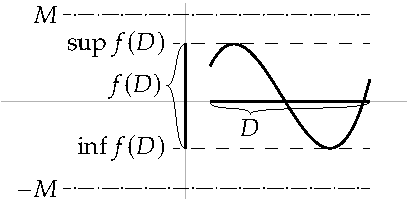
\includegraphics{figures/boundedfunc}
\caption{Example of a bounded function, a bound $M$, and its supremum and infimum.\label{boundedfuncfig}}
\end{myfigureht}
For a function $f \colon D \to \R$ we write
(see \figureref{boundedfuncfig} for
an example)
\glsadd{not:supf}\glsadd{not:inff}
\begin{align*}
& \sup_{x \in D} f(x) := \sup\, f(D) , \\
& \inf_{x \in D} f(x) := \inf\, f(D) .
\end{align*}
We also sometimes replace the \myquote{$x \in D$} with an expression.
For example if, as before, $f(x) = x^2-9x+1$, for $-1 \leq x \leq 5$, 
a little bit of calculus shows
\begin{equation*}
\sup_{x \in D} f(x) = 
\sup_{-1 \leq x \leq 5} ( x^2 -9x+1 ) = 11,
\qquad
\inf_{x \in D} f(x) = 
\inf_{-1 \leq x \leq 5} ( x^2 -9x+1 ) = \nicefrac{-77}{4} .
\end{equation*}



\begin{prop} \label{prop:funcsupinf}
If $f \colon D \to \R$ and $g \colon D \to \R$ ($D$ nonempty) are
bounded\footnote{The boundedness hypothesis is for simplicity,
it can be dropped if we allow for the extended real numbers.}
functions and
\begin{equation*}
f(x) \leq g(x) \qquad \text{for all } x \in D,
\end{equation*}
then
\begin{equation} \label{prop:funcsupinf:eq}
\sup_{x \in D} f(x) \leq \sup_{x \in D} g(x)
\qquad \text{and} \qquad
\inf_{x \in D} f(x) \leq \inf_{x \in D} g(x) .
\end{equation}
\end{prop}

You should be careful with the variables.  The $x$ on the left side of
the inequality in \eqref{prop:funcsupinf:eq}
is different from the $x$ on the right.  You
should really think of the first inequality as
\begin{equation*}
\sup_{x \in D} f(x) \leq \sup_{y \in D} g(y) .
\end{equation*}
Let us prove this inequality.  If $b$ is an upper bound for $g(D)$, then
$f(x) \leq g(x) \leq b$ for all $x \in D$, and hence $b$ is an upper bound for $f(D)$.
Taking the least upper bound we get that for all $x \in D$
\begin{equation*}
f(x) \leq \sup_{y \in D} g(y) .
\end{equation*}
Therefore
$\sup_{y \in D} g(y)$ is an upper bound for $f(D)$ and thus greater than or
equal to the least upper bound of $f(D)$.
\begin{equation*}
\sup_{x \in D} f(x) \leq \sup_{y \in D} g(y) .
\end{equation*}
The second inequality (the statement about the inf) is left as an exercise.

\medskip

A common mistake is to conclude 
\begin{equation} \label{rn:av:ltnottrue}
\sup_{x \in D} f(x) \leq \inf_{y \in D} g(y) .
\end{equation}
The inequality \eqref{rn:av:ltnottrue} is not true given the hypothesis of
the proposition above.  For this stronger
inequality we need the stronger hypothesis
\begin{equation*}
f(x) \leq g(y) \qquad \text{for all } x \in D \text{ and } y \in D.
\end{equation*}
The proof as well as a counterexample is left as an exercise.

\subsection{Exercises}

\begin{exercise}
Show that
$\abs{x-y} < \epsilon$ if and only if $x-\epsilon < y < x+\epsilon$.
\end{exercise}

\begin{exercise}
Show: \qquad
%\begin{enumerate}[a)]
%\item
a)
$\max \{x,y\} = \frac{x+y+\abs{x-y}}{2}$
%\item
\qquad
b)
$\min \{x,y\} = \frac{x+y-\abs{x-y}}{2}$
%\end{enumerate}
\end{exercise}

\begin{exercise}
Find a number $M$ such that $\sabs{x^3-x^2+8x} \leq M$ for all $-2 \leq x \leq
10$.
\end{exercise}

\begin{exercise}
Finish the proof of \propref{prop:funcsupinf}.
That is, prove that
given any set $D$,
and two bounded functions
$f \colon D \to \R$ and $g \colon D \to \R$ 
such that $f(x) \leq g(x)$ for all $x \in D$, then 
\begin{equation*}
\inf_{x\in D} f(x) \leq \inf_{x\in D} g(x) .
\end{equation*}
\end{exercise}

\begin{exercise}
Let 
$f \colon D \to \R$ and $g \colon D \to \R$ be functions ($D$ nonempty).
\begin{enumerate}[a)]
%
\item
Suppose 
$f(x) \leq g(y)$ for all $x \in D$ and $y \in D$.  Show that
\begin{equation*}
\sup_{x\in D} f(x) \leq \inf_{x\in D} g(x) .
\end{equation*}
%
\item
Find a specific $D$, $f$, and $g$, such that
$f(x) \leq g(x)$ for all $x \in D$, but
\begin{equation*}
\sup_{x\in D} f(x) > \inf_{x\in D} g(x) .
\end{equation*}
\end{enumerate}
\end{exercise}

\begin{exercise}
Prove \propref{prop:funcsupinf} without the assumption that
the functions are bounded.  Hint: You need to use the extended real
numbers.
\end{exercise}

\begin{exercise} \label{exercise:sumofsup}
Let $D$ be a nonempty set.
Suppose $f \colon D \to \R$ and $g \colon D \to \R$ are bounded functions.
\begin{enumerate}[a)]
\item
Show 
\begin{equation*}
\sup_{x\in D} \bigl(f(x) + g(x) \bigr) \leq
\sup_{x\in D} f(x)
+
\sup_{x\in D} g(x)
\qquad \text{and} \qquad
\inf_{x\in D} \bigl(f(x) + g(x) \bigr) \geq
\inf_{x\in D} f(x)
+
\inf_{x\in D} g(x) .
\end{equation*}
\item
Find examples where we obtain strict inequalities.
\end{enumerate}
\end{exercise}

\begin{exercise}
Suppose $f \colon D \to \R$ and $g \colon D \to \R$ are bounded functions
and
$\alpha \in \R$.
\begin{enumerate}[a)]
\item
Show that $\alpha f \colon D \to \R$ defined by $(\alpha f) (x) := \alpha
f(x)$ is a bounded function.
\item
Show that $f+g \colon D \to \R$ defined by $(f+g) (x) := f(x) + g(x)$
is a bounded function.
\end{enumerate}
\end{exercise}

\begin{exercise}
Let $f \colon D \to \R$ and $g \colon D \to \R$ be functions, $\alpha \in
\R$, and
recall what $f+g$ and $\alpha f$ means from the previous exercise.
\begin{enumerate}[a)]
\item
Prove that if $f+g$ and $g$ are bounded, then $f$ is bounded.
\item
Find an example where $f$ and $g$ are both unbounded, but $f+g$ is
bounded.
\item
Prove that if $f$ is bounded but $g$ is unbounded, then $f+g$ is
unbounded.
\item
Find an example where $f$ is unbounded but $\alpha f$ is bounded.
\end{enumerate}
\end{exercise}

%%%%%%%%%%%%%%%%%%%%%%%%%%%%%%%%%%%%%%%%%%%%%%%%%%%%%%%%%%%%%%%%%%%%%%%%%%%%%%

\sectionnewpage
\section{Intervals and the size of \texorpdfstring{$\R$}{R}}
\label{sec:intandsizeR}

\sectionnotes{0.5--1 lecture (proof of uncountability of $\R$ can be optional)}

You surely saw the notation for intervals\index{interval}
before, but let us give a formal
definition here.  For $a,  b \in \R$ such that $a < b$ we define
\glsadd{not:openbdinterval}%
\glsadd{not:closedbdinterval}%
\glsadd{not:halfopenbdinterval}%
\glsadd{not:openubdinterval}%
\glsadd{not:closedubdinterval}%
\begin{align*}
& [a,b] := \{ x \in \R : a \leq x \leq b \}, \\
& (a,b) := \{ x \in \R : a < x < b \}, \\
& (a,b] := \{ x \in \R : a < x \leq b \}, \\
& [a,b) := \{ x \in \R : a \leq x < b \} .
\end{align*}
The interval $[a,b]$ is called a \emph{\myindex{closed interval}}
and $(a,b)$ is called an \emph{\myindex{open interval}}.  The intervals
of the form $(a,b]$ and $[a,b)$ are called
\emph{half-open intervals}\index{half-open interval}.

The intervals above were all \emph{bounded intervals}\index{bounded
interval}, since both $a$ and $b$ were real numbers.  We 
define \emph{unbounded intervals}\index{unbounded interval},
\begin{align*}
& [a,\infty) := \{ x \in \R : a \leq x \}, \\
& (a,\infty) := \{ x \in \R : a < x \}, \\
& (-\infty,b] := \{ x \in \R : x \leq b \}, \\
& (-\infty,b) := \{ x \in \R : x < b \} .
\end{align*}
For completeness, we define $(-\infty,\infty) := \R$.
The intervals $[a,\infty)$, $(-\infty,b]$, and $\R$ are sometimes called
\emph{\myindex{unbounded closed intervals}},
and $(a,\infty)$, $(-\infty,b)$, and $\R$ are sometimes called
\emph{\myindex{unbounded open intervals}}.

In short, an interval is a set with at least two points
that contains all points between any two
points.\footnote{Sometimes single point sets and the empty set are
also called intervals, but in this book, intervals have at least 2 points.}
The proof of the following proposition is left as an exercise.

\begin{prop} \label{prop:intervaldef}
A set $I \subset \R$ is an interval if and only if
$I$ contains at least 2 points and
for all $a,c \in I$ and $b \in \R$ such that $a < b < c$ we have $b \in I$.
\end{prop}

We have already seen that any open interval $(a,b)$ (where $a < b$ of course)
must be nonempty.  For example, it contains the number $\frac{a+b}{2}$.
An unexpected fact is that from a set-theoretic perspective,
all intervals have the same \myquote{size,} that is, they all have
the same cardinality.  For example the map $f(x) := 2x$
takes the interval $[0,1]$ bijectively to the interval $[0,2]$.

Maybe more interestingly,
the function $f(x) := \tan(x)$
is a bijective map from $(-\nicefrac{\pi}{2},\nicefrac{\pi}{2})$ to $\R$.  Hence the bounded
interval $(-\nicefrac{\pi}{2},\nicefrac{\pi}{2})$ has the same cardinality as $\R$.  It is not
completely straightforward to construct a bijective map from $[0,1]$ to
$(0,1)$, but it is possible.

And do not worry, there does exist a way to measure the \myquote{size} of subsets
of real numbers that
\myquote{sees}
the difference between $[0,1]$ and $[0,2]$.  However, its proper definition
requires much more machinery than we have right now.

Let us say more about the cardinality of intervals and hence about the
cardinality of $\R$.  We have seen that there exist irrational numbers, that is
$\R \setminus \Q$ is nonempty.  The question is: How many irrational numbers
are there?  It turns out there are a lot more irrational numbers than rational
numbers.  We have seen that $\Q$ is countable, and we will show 
that $\R$ is uncountable.
In fact, the cardinality of $\R$ is the
same as the cardinality of $\sP(\N)$, although we will not prove this
claim here.

\begin{thm}[Cantor]\index{Cantor's theorem}
$\R$ is uncountable.
\end{thm}

We give a modified version of
Cantor's original proof from
1874 as this proof requires the least setup.  Normally this proof is stated
as a contradiction proof, but a proof by contrapositive is easier to
understand.

\begin{proof}
Let $X \subset \R$ be a countably infinite
subset such that for any two real numbers
$a < b$, there is an $x \in X$ such that $a < x < b$.  Were $\R$ countable,
then we could take $X = \R$.  If we show that $X$ is necessarily
a proper subset, then $X$ cannot equal $\R$, and $\R$ must be
uncountable.

As $X$ is countably infinite, 
there is a bijection from $\N$ to $X$.  Consequently, we write $X$ as
a sequence of real numbers $x_1, x_2, x_3,\ldots$, such that
each number in $X$
is given by $x_j$ for some $j \in \N$.

Let us inductively
construct two sequences of real numbers $a_1,a_2,a_3,\ldots$ and
$b_1,b_2,b_3,\ldots$.  Let
$a_1 := x_1$ and $b_1 := x_1+1$.  Note that $a_1 < b_1$ and
$x_1 \notin (a_1,b_1)$.
For $k > 1$, suppose $a_{k-1}$ and $b_{k-1}$ have been defined.
Let us also suppose $(a_{k-1},b_{k-1})$ does not contain any $x_j$
for any $j=1,\ldots,k-1$.
\begin{enumerate}[(i)]
\item Define $a_k := x_j$, where $j$ is the smallest $j \in \N$
such that $x_j \in (a_{k-1},b_{k-1})$.  Such an $x_j$ exists by our
assumption on $X$.  
\item Next, define $b_k := x_j$ where $j$ is the smallest $j \in \N$
such that $x_j \in (a_{k},b_{k-1})$.
\end{enumerate}
Notice that $a_k < b_k$ and $a_{k-1} < a_k < b_k < b_{k-1}$.
Also notice that $(a_{k},b_{k})$ does not contain $x_k$ and hence
does not contain any $x_j$ for $j=1,\ldots,k$.

Claim: \emph{$a_j < b_k$ for all $j$ and $k$ in $\N$.}  Let us first
assume $j < k$.  Then $a_j < a_{j+1} < \cdots < a_{k-1} < a_k < b_k$.
Similarly for $j > k$.  The claim follows.

Let $A = \{ a_j : j \in \N \}$ and $B = \{ b_j : j \in \N \}$.
By \propref{infsupineq:prop} and the claim above we have
\begin{equation*}
\sup\, A \leq \inf\, B .
\end{equation*}
Define $y := \sup\, A$.  The number $y$ cannot be a member of $A$.  If $y = a_j$
for some $j$, then $y < a_{j+1}$, which is impossible.
Similarly, $y$ cannot be a member of $B$.  Therefore,
$a_j < y$ for all $j\in \N$
and $y < b_j$ for all $j\in \N$.
In other words $y \in (a_j,b_j)$ for all $j\in \N$.

Finally, we must show that $y \notin X$.  If we do so, then we will have
constructed a real number not in $X$ showing that $X$ must have been a
proper subset.  Take any $x_k \in X$.  By the construction above
$x_k \notin (a_k,b_k)$, so $x_k \not= y$ as $y \in (a_k,b_k)$.

Therefore, the sequence $x_1,x_2,\ldots$ cannot contain all elements of $\R$
and thus $\R$ is uncountable.
\end{proof}

\subsection{Exercises}

\begin{exercise}
For $a < b$, construct an explicit bijection from $(a,b]$ to $(0,1]$.
\end{exercise}

\begin{exercise}
Suppose $f \colon [0,1] \to (0,1)$ is a bijection.
Using $f$, construct a
bijection from $[-1,1]$ to $\R$.
\end{exercise}

\begin{exercise} \label{exercise:intervaldef}
Prove \propref{prop:intervaldef}.
That is,
suppose $I \subset \R$ is a subset with at least 2 elements
such that if $a < b < c$ and $a, c \in I$, then $b \in I$.
Prove that $I$ is one of the nine types of intervals explicitly
given in this section.
Furthermore, prove that the intervals given in this section
all satisfy this property.
\end{exercise}

\begin{exercise}[Hard]
Construct an explicit bijection from $(0,1]$ to $(0,1)$.
Hint: One approach is as follows: First map $(\nicefrac{1}{2},1]$
to $(0,\nicefrac{1}{2}]$, then map
$(\nicefrac{1}{4},\nicefrac{1}{2}]$
to $(\nicefrac{1}{2},\nicefrac{3}{4}]$, etc.
Write down the map explicitly, that
is, write down an algorithm that tells you exactly what number goes where.
Then prove that the map is a bijection.
\end{exercise}

\begin{exercise}[Hard]
Construct an explicit bijection from $[0,1]$ to $(0,1)$.
\end{exercise}

\begin{exercise}
\leavevmode
\begin{enumerate}[a)]
\item
Show that every closed interval $[a,b]$ is the intersection
of countably many open intervals.
\item
Show that every open interval $(a,b)$
is a countable union of closed intervals.
\item
Show that an intersection
of a possibly infinite family of bounded closed intervals,
$\bigcap\limits_{\lambda \in I} [a_\lambda,b_\lambda]$,
is either empty, a single point,
or a bounded closed interval.
\end{enumerate}
\end{exercise}

\begin{exercise}
Suppose $S$ is a set of disjoint open intervals in $\R$.  That is, 
if $(a,b) \in S$ and $(c,d) \in S$, then either $(a,b) = (c,d)$
or $(a,b) \cap (c,d) = \emptyset$.  Prove $S$ is a countable set.
\end{exercise}

\begin{exercise}
Prove that the cardinality of $[0,1]$ is the same as the cardinality of
$(0,1)$ by showing that
$\abs{[0,1]} \leq \abs{(0,1)}$ and
$\abs{(0,1)} \leq \abs{[0,1]}$.  See 
\defnref{def:comparecards}.
This proof requires the Cantor--Bernstein--Schr\"oder theorem we
stated without proof.  Note that this proof does not give you an
explicit bijection.
\end{exercise}

\begin{exercise}[Challenging]
A number $x$ is \emph{algebraic}\index{algebraic number} if $x$ is a root of a polynomial with
integer coefficients, in other words, $a_n x^n + a_{n-1} x^{n-1}  + \cdots
+ a_1 x + a_0 = 0$ where all $a_n \in \Z$.
\begin{enumerate}[a)]
\item
Show that there are only
countably many algebraic numbers.
\item
Show that there exist non-algebraic
numbers (follow in the footsteps of Cantor, use uncountability of $\R$).
\end{enumerate}
Hint: Feel free to use the fact that a polynomial of degree $n$ has at most $n$ real
roots.
\end{exercise}

\begin{exercise}[Challenging]
Let $F$ be the set of all functions $f \colon \R \to \R$.
Prove $\abs{\R} < \abs{F}$
using Cantor's \thmref{cantorspowersetthm}.\footnote{Interestingly,
if $C$ is the set of continuous functions, then $\abs{\R} = \abs{C}$.}
\end{exercise}

%%%%%%%%%%%%%%%%%%%%%%%%%%%%%%%%%%%%%%%%%%%%%%%%%%%%%%%%%%%%%%%%%%%%%%%%%%%%%%

\sectionnewpage
\section{Decimal representation of the reals}
\label{sec:decimals}

\sectionnotes{1 lecture (optional)}

We often think of real numbers as their
\emph{\myindex{decimal representation}}.  For
a positive integer $n$, we find the digits $d_K,d_{K-1},\ldots,d_2,d_1,d_0$ for some
$K$,
where each $d_j$ is an integer between $0$ and $9$, then
\begin{equation*}
n = d_K {10}^K + d_{K-1} {10}^{K-1} + \cdots + d_2 {10}^2 + d_1 10 + d_0 .
\end{equation*}
We often assume $d_K \not= 0$.  To represent $n$ we write the sequence of
digits: $n = d_K d_{K-1} \cdots d_2 d_1 d_0$.
By a (decimal)
\emph{\myindex{digit}}\index{decimal digit}, we mean an integer
between $0$ and $9$.

Similarly, we
represent some rational numbers.  That is, for certain
numbers $x$, we can find
negative integer $-M$, a positive integer $K$, and digits
$d_K,d_{K-1},\ldots,d_1,d_0,d_{-1},\ldots,d_{-M}$, such that
\begin{equation*}
x = d_K {10}^K + d_{K-1} {10}^{K-1} + \cdots + d_2 {10}^2 + d_1 10 + d_0 
+ d_{-1} {10}^{-1} + d_{-2} {10}^{-2} + \cdots + d_{-M} {10}^{-M} .
\end{equation*}
We write $x = d_K d_{K-1} \cdots d_1 d_0 \, . \, d_{-1} d_{-2} \cdots d_{-M}$.

Not every real number has such a representation, even the simple
rational number $\nicefrac{1}{3}$ does not.  The irrational number $\sqrt{2}$ 
does not have such a representation either.  To get a representation for
all real numbers we must allow infinitely many digits.

Let us consider only real numbers in the interval $(0,1]$.  If
we find a representation for these, adding 
integers to them obtains a representation for all real numbers.
Take an infinite sequence of decimal digits:
\begin{equation*}
0.d_1d_2d_3\ldots.
\end{equation*}
That is, we have a digit $d_j$ for every $j \in \N$.
We renumbered the digits to avoid the negative signs.
We call the number
\begin{equation*}
D_n := 
\frac{d_1}{10} + 
\frac{d_2}{{10}^2} + 
\frac{d_3}{{10}^3} + 
\cdots +
\frac{d_n}{{10}^n} .
\end{equation*}
the truncation of $x$ to $n$ decimal digits.
We say this
sequence of digits represents a real number $x$ if
\begin{equation*}
x =
\sup_{n \in \N} \left(
\frac{d_1}{10} + 
\frac{d_2}{{10}^2} + 
\frac{d_3}{{10}^3} + 
\cdots +
\frac{d_n}{{10}^n}
\right) =
\sup_{n \in \N} \, D_n .
\end{equation*}

\begin{prop} \label{prop:decimalprop}
{~}
\begin{enumerate}[(i)]
\item
Every infinite sequence of digits
$0.d_1d_2d_3\ldots$ represents a unique real number $x \in [0,1]$, and
\begin{equation*}
D_n \leq x \leq D_n+\frac{1}{{10}^n} \qquad \text{for all } n \in \N.
\end{equation*}
\item
For every $x \in (0,1]$ there exists an infinite sequence of digits
$0.d_1d_2d_3\ldots$ that represents $x$.
There exists a unique representation such that
\begin{equation*}
D_n < x \leq D_n+\frac{1}{{10}^n} \qquad \text{for all } n \in \N.
\end{equation*}
\end{enumerate}
\end{prop}

\begin{proof}
Let us start with the first item.  Take an arbitrary infinite sequence of
digits $0.d_1d_2d_3\ldots$.  Use the geometric sum formula to write
\begin{equation*}
\begin{split}
D_n =
\frac{d_1}{10} + 
\frac{d_2}{{10}^2} + 
\frac{d_3}{{10}^3} + 
\cdots +
\frac{d_n}{{10}^n} 
& \leq
\frac{9}{10} + 
\frac{9}{{10}^2} + 
\frac{9}{{10}^3} + 
\cdots +
\frac{9}{{10}^n} 
\\
& =
\frac{9}{10}
\bigl( 1 + \nicefrac{1}{10} + 
{(\nicefrac{1}{10})}^2 + \cdots + 
{(\nicefrac{1}{10})}^{n-1} \bigr)
\\
& =
\frac{9}{10}
\left(
\frac{1-{(\nicefrac{1}{10})}^{n}}{1-\nicefrac{1}{10}}
\right)
= 1-{(\nicefrac{1}{10})}^{n}
< 1 .
\end{split}
\end{equation*}
In particular, $D_n < 1$ for all $n$.  A sum of nonnegative numbers is
nonnegative so $D_n \geq 0$, and hence
\begin{equation*}
0 \leq \sup_{n\in \N} \, D_n \leq 1 .
\end{equation*}
Therefore, $0.d_1d_2d_3\ldots$ represents a unique number $x := \sup_{n\in
\N} D_n \in [0,1]$.
As $x$ is a supremum, then $D_n \leq x$.
Take $m \in \N$.  If $m < n$, then $D_m - D_n \leq 0$.  If $m > n$, then
computing as above
\begin{equation*}
D_m - D_n
=
\frac{d_{n+1}}{{10}^{n+1}} + 
\frac{d_{n+2}}{{10}^{n+2}} + 
\frac{d_{n+3}}{{10}^{n+3}} + 
\cdots +
\frac{d_{m}}{{10}^m} 
\leq
\frac{1}{{10}^{n}}
\bigl(
1-{(\nicefrac{1}{10})}^{m-n}
\bigr)
<
\frac{1}{{10}^{n}} .
\end{equation*}
Take the supremum over $m$ to find
\begin{equation*}
x - D_n
\leq
\frac{1}{{10}^{n}} .
\end{equation*}

We move on to the
second item.  Take any $x \in (0,1]$.
First let us tackle the existence.
For convenience let $D_0 := 0$.
Then,
$D_0 < x \leq D_0 + {10}^{-0}$.
Suppose we defined the digits $d_1,d_2,\ldots,d_n$,
and that 
$D_k < x \leq D_k + {10}^{-k}$, for $k=0,1,2,\ldots,n$.  We need to define $d_{n+1}$.

By the 
\hyperref[thm:arch:i]{Archimedean property} of the real numbers,
find an integer $j$ such that
$x-D_n \leq j {10}^{-(n+1)}$.  Take the least such $j$ and obtain 
\begin{equation} \label{eq:theDnjineq}
(j-1){10}^{-(n+1)} < x-D_n \leq j {10}^{-(n+1)} .
\end{equation}
Let $d_{n+1} := j-1$.
As $D_n < x$,
then $d_{n+1} = j-1 \geq 0$.  On the other hand since
$x-D_n \leq {10}^{-n}$ we have that
$j$ is at most 10, and therefore $d_{n+1} \leq 9$.
So $d_{n+1}$ is a
decimal digit.
Since $D_{n+1} = D_n + d_{n+1} {10}^{-(n+1)}$
add $D_n$ to the inequality
\eqref{eq:theDnjineq} above:
\begin{multline*}
D_{n+1} = D_n + (j-1){10}^{-(n+1)} < x
\leq
D_n + j {10}^{-(n+1)} \\
=
D_n + (j-1) {10}^{-(n+1)} +
{10}^{-(n+1)} = D_{n+1} + {10}^{-(n+1)} .
\end{multline*}
And so
$D_{n+1} < x \leq D_{n+1} + {10}^{-(n+1)}$ holds.
We inductively
defined an infinite sequence of digits $0.d_1d_2d_3\ldots$.

Consider $D_{n} < x \leq D_{n} + {10}^{-n}$.
As $D_n < x$ for all $n$, then
$\sup \{ D_n : n \in \N \} \leq x$.
The second inequality for $D_n$ implies
\begin{equation*}
x - \sup \{ D_m : m \in \N \}
\leq
x - D_n \leq 10^{-n} .
\end{equation*}
As the inequality holds for all $n$ and
${10}^{-n}$ can be made arbitrarily small (see
\exerciseref{exercise:bnlimit}) we have $x \leq 
\sup \{ D_m : m \in \N \}$.
Therefore
$\sup \{ D_m : m \in \N \} = x$.

What is left to show is the uniqueness.
Suppose $0.e_1e_2e_3\ldots$ is another representation of $x$.
Let $E_n$ be the $n$-digit truncation of $0.e_1e_2e_3\ldots$, and suppose
$E_n < x \leq E_n + {10}^{-n}$ for all $n \in \N$.
Suppose for some $K \in \N$, $e_n = d_n$ for all $n < K$, so
$D_{K-1} = E_{K-1}$.  Then
\begin{equation*}
E_K = D_{K-1} + e_K{10}^{-K} < x \leq E_K + {10}^{-K} = D_{K-1} +
e_K{10}^{-K} + {10}^{-K} .
\end{equation*}
Subtracting $D_{K-1}$ and multiplying by ${10}^{K}$ we get
\begin{equation*}
e_K < (x - D_{K-1}){10}^K \leq e_K + 1 .
\end{equation*}
Similarly,
\begin{equation*}
d_K < (x - D_{K-1}){10}^K \leq d_K + 1 .
\end{equation*}
Hence, both $e_K$ and $d_K$ are the largest integer $j$
such that $j < (x - D_{K-1}){10}^K$, and therefore $e_K = d_K$.  That is,
the representation is unique.
\end{proof}

The representation is not unique if we do not require
$D_n < x$ for all $n$.
For example, for the
number $\nicefrac{1}{2}$ the method in the proof obtains the representation
\begin{equation*}
0.49999\ldots .
\end{equation*}
However, we also have the representation $0.50000\ldots$.

The only numbers that have nonunique
representations are ones that end either in an infinite sequence of $0$s
or $9$s, because the only representation for which
$D_n = x$ is one where all digits past the $n$th digit are zero.  In this case
there are exactly two representations of $x$ (see the exercises).

Let us give another proof of the uncountability of the reals using decimal
representations.
This is Cantor's second proof, and is probably better known.
This proof may seem shorter, but it is because we already did
the hard part above and we are left with a slick trick to prove that $\R$ is
uncountable.  This trick is called
\emph{\myindex{Cantor diagonalization}}\index{diagonalization} and
finds use in other proofs as well.

\begin{thm}[Cantor]
The set $(0,1]$ is uncountable.
\end{thm}

\begin{proof}
Let $X := \{ x_1,x_2,x_3,\ldots \}$ be any countable subset of real numbers in $(0,1]$.
We will construct a real number not in $X$.  Let
\begin{equation*}
x_n = 0.d_1^nd_2^nd_3^n\ldots
\end{equation*}
be the unique representation from the proposition, that is, $d_j^n$ is the
$j$th digit of the $n$th number.  Let
\begin{equation*}
e_n :=
\begin{cases}
1 & \text{if } d_n^n \not= 1, \\
2 & \text{if } d_n^n = 1.
\end{cases}
\end{equation*}
Let $E_n$ be the $n$-digit truncation of $y = 0.e_1e_2e_3\ldots$.  Because
all the digits are nonzero we get $E_n < E_{n+1} \leq y$.  Therefore
\begin{equation*}
E_n < y \leq E_n + {10}^{-n} 
\end{equation*}
for all $n$, and the representation is the unique one for $y$ from 
the proposition.  For every $n$, the $n$th digit
of $y$ is different from the $n$th digit of $x_n$, so $y \not= x_n$.
Therefore $y \notin X$, and as $X$ was an arbitrary countable subset,
$(0,1]$ must be uncountable.  See \figureref{cantorexamplefig} for an
example.
\begin{myfigureht}
\subimport*{figures/}{cantorexamplefig.pdf_t}
\caption{Example of Cantor diagonalization, the diagonal digits $d_n^n$
marked.\label{cantorexamplefig}}
\end{myfigureht}
\end{proof}

Using decimal digits we can also find lots of numbers that are not rational.
The following proposition is true for every
rational number, but we give it only for $x \in (0,1]$ for simplicity.

\begin{prop} \label{prop:rationaldecimal}
If $x \in (0,1]$ is a rational number and $x = 0.d_1d_2d_3\ldots$,
then the decimal digits eventually start repeating.  That is, there are 
positive integers $N$ and $P$, such that for all $n \geq N$, $d_n = d_{n+P}$.
\end{prop}

\begin{proof}
Let $x = \nicefrac{p}{q}$ for positive integers $p$ and $q$.
Suppose $x$ is a number with a unique representation, as
otherwise we have seen above that both its representations are repeating,
see also \exerciseref{exercise:nonuniquedecimals}.  This also means
that $x \not= 1$ so $p < q$.

To compute the first digit we take $10 p$ and divide by
$q$.  Let $d_1$ be the quotient, and the remainder $r_1$ is some integer
between 0 and $q-1$.  That is, $d_1$ is the largest integer
such that $d_1 q \leq 10p$ and then $r_1 = 10p - d_1q$.
As $p < q$, then $d_1 < 10$, so $d_1$ is a digit.
Furthermore,
\begin{equation*}
\frac{d_1}{10} \leq \frac{p}{q} =
\frac{d_1}{10} + \frac{r_1}{10q} \leq \frac{d_1}{10} +
\frac{1}{10} .
\end{equation*}
The first inequality must be strict since $x$ has a
unique representation.  That is, $d_1$ really is the first digit.
What is left is $\nicefrac{r_1}{(10q)}$.  This is the same as computing the
first digit of $\nicefrac{r_1}{q}$.
To compute $d_2$ divide $10 r_1$ by $q$, and so on.
After computing $n-1$ digits, we have
$\nicefrac{p}{q} = D_{n-1} + \nicefrac{r_{n-1}}{(10^{n} q)}$.
To get the $n$th digit,
divide $10 r_{n-1}$ by $q$
to get quotient $d_n$, remainder $r_n$, and the inequalities
\begin{equation*}
\frac{d_n}{10} \leq \frac{r_{n-1}}{q} =
\frac{d_n}{10} + \frac{r_n}{10q} \leq \frac{d_n}{10} +
\frac{1}{10} .
\end{equation*}
Dividing by $10^{n-1}$ and adding $D_{n-1}$ we find
\begin{equation*}
D_n \leq D_{n-1} + \frac{r_{n-1}}{10^{n} q} = \frac{p}{q} \leq D_n +
\frac{1}{10^n} .
\end{equation*}
By uniqueness we really have 
the $n$th digit $d_n$ from the construction.

The new digit depends only the remainder from the previous
step.  There
are at most $q$ possible remainders
and hence at some step the process must start repeating itself,
and $P$ is at most $q$.
\end{proof}

The converse of the proposition is also true and is left as an exercise.

\begin{example}
The number
\begin{equation*}
x = 0.101001000100001000001\ldots,
\end{equation*}
is irrational.
That is, the digits are $n$ zeros, then a one, then $n+1$
zeros, then a one, and so on and so forth.
The fact that $x$ is irrational follows from the
proposition; the digits never start repeating.
For every $P$,
if we go far enough, we find a 1 followed by at least $P+1$ zeros.
\end{example}

\subsection{Exercises}

\begin{exercise}[Easy]
What is the decimal representation of $1$ guaranteed by
\propref{prop:decimalprop}?  Make sure to show that it does satisfy
the condition.
\end{exercise}

\begin{exercise}
Prove the converse of \propref{prop:rationaldecimal}, that is,
if the digits in the decimal representation of $x$ are eventually repeating, then 
$x$ must be rational.
\end{exercise}

\begin{exercise} \label{exercise:nonuniquedecimals}
Show that real numbers $x \in (0,1)$ with nonunique decimal representation
are exactly the rational numbers that can be written
as $\frac{m}{10^n}$ for some integers $m$ and $n$.  In this case show that
there exist exactly two representations of $x$.
\end{exercise}

\begin{exercise} \label{exercise:decimalpropbaseb}
Let $b \geq 2$ be an integer.  Define a representation of a real number in
$[0,1]$ in terms of base $b$ rather than base 10 and prove
\propref{prop:decimalprop} for base $b$.
\end{exercise}

\begin{exercise}
Using the previous exercise with $b=2$ (binary), 
show that cardinality of $\R$ is the same as the cardinality of $\sP(\N)$,
obtaining yet another (though related) proof that $\R$ is uncountable.
Hint: Construct two injections, one from $[0,1]$ to $\sP(\N)$
and one from $\sP(\N)$ to $[0,1]$.  Hint 2: Given a
set $A \subset \N$, let the $n$th binary digit of $x$ be 1 if $n\in A$.
\end{exercise}

\begin{exercise}[Challenging]
Construct a bijection between $[0,1]$ and $[0,1] \times [0,1]$.\footnote{%
If you can't do it, try to at least construct an injection from
$[0,1] \times [0,1]$ to
$[0,1]$.}
Hint:
Consider even and odd digits to construct a bijection between 
$[0,1] \setminus A$ and $[0,1] \times [0,1]$ for a countable set $A$ (be
careful about uniqueness of representation).
Then construct a bijection between $([0,1] \times [0,1]) \setminus B$
and $[0,1] \times [0,1]$ for a countable set $B$ (e.g.\ use 
that $\N$ and the even natural numbers are bijective).
\end{exercise}

\begin{exercise}
Prove that if $x = \nicefrac{p}{q} \in (0,1]$ is a rational number, $q > 1$,
then the period $P$ of repeating digits in the decimal representation
of $x$ is in fact less than or equal to $q-1$.
\end{exercise}

\begin{exercise} \label{exercise:bnlimit}
Prove that if $b \in \N$ and $b \geq 2$, then for any $\epsilon > 0$,
there is an $n \in \N$ such that 
we have $b^{-n} < \epsilon$.  Hint:
One possibility is to first prove that $b^n > n$ for all $n \in \N$ by induction.
\end{exercise}

\begin{exercise}
Explicitly construct an injection $f \colon \R \to \R \setminus \Q$ using
\propref{prop:rationaldecimal}.
\end{exercise}


%%%%%%%%%%%%%%%%%%%%%%%%%%%%%%%%%%%%%%%%%%%%%%%%%%%%%%%%%%%%%%%%%%%%%%%%%%%%%%

% Sequences and Series chapter
\chapter{Sequences and Series} \label{seq:chapter}

%%%%%%%%%%%%%%%%%%%%%%%%%%%%%%%%%%%%%%%%%%%%%%%%%%%%%%%%%%%%%%%%%%%%%%%%%%%%%%

\section{Sequences and limits}
\label{sec:seqsandlims}

\sectionnotes{2.5 lectures}

Analysis is essentially about taking limits.  The most basic type of a limit
is a limit of a sequence of real numbers.
We have already seen sequences used informally.  Let us give the formal
definition.

\begin{defn}
A \emph{\myindex{sequence}} (of real numbers) is a function $x \colon \N \to
\R$.  Instead of $x(n)$, we 
usually denote the $n$th element in the sequence by $x_n$.  We 
use the notation $\{ x_n \}$, or more precisely
\begin{equation*}
\{ x_n \}_{n=1}^\infty,
\end{equation*}
\glsadd{not:sequence}
to denote a sequence.

A sequence $\{ x_n \}$ is \emph{bounded}\index{bounded sequence} if
there exists a $B \in \R$ such that
\begin{equation*}
\abs{x_n} \leq B \qquad \text{for all } n \in \N.
\end{equation*}
In other words, the sequence $\{x_n\}$ is bounded whenever
the set $\{ x_n : n \in \N \}$
is bounded, or equivalently when it is bounded as a function.
\end{defn}

When we need
to give a concrete sequence we often give each term as a formula in
terms of $n$.
For example, $\{ \nicefrac{1}{n} \}_{n=1}^\infty$, or simply $\{
\nicefrac{1}{n} \}$, stands for
the sequence $1, \nicefrac{1}{2}, \nicefrac{1}{3}, \nicefrac{1}{4},
\nicefrac{1}{5}, \ldots$.
The sequence $\{ \nicefrac{1}{n} \}$
is a bounded sequence ($B=1$ suffices).  On the other hand the sequence $\{ n \}$ stands for
$1,2,3,4,\ldots$, and this sequence is not bounded (why?).

While the notation for a sequence
is similar\footnote{\cite{BS} use the notation $(x_n)$ to denote
a sequence instead of $\{ x_n \}$, which is what \cite{Rudin:baby} uses.
Both are common.}
to that of a set, the notions are
distinct.  For example, the sequence $\{ {(-1)}^n \}$ is the sequence
$-1,1,-1,1,-1,1,\ldots$, whereas the set of values, the
\emph{range of the sequence}\index{range of a sequence},
is just the set $\{ -1, 1 \}$.  We can write this set
as $\{ {(-1)}^n : n \in \N \}$.   When ambiguity can arise, we
use the words \emph{sequence} or \emph{set} to distinguish the two
concepts.

Another example of a sequence is the so-called \emph{\myindex{constant sequence}}.
That is a sequence $\{ c \} = c,c,c,c,\ldots$ consisting of a single
constant $c \in \R$ repeating indefinitely.

We now get to the idea of a
\emph{limit of a sequence}\index{limit!of a sequence}.  We will
see in \propref{prop:limisunique}
that the notation below is well-defined.  That is, if a limit exists, then
it is unique.  So it makes sense to talk about \emph{the} limit of a sequence.

\begin{defn}
A sequence $\{ x_n \}$ is said to \emph{converge} to a number
$x \in \R$, if for every $\epsilon > 0$, there exists an $M \in \N$ such
that $\abs{x_n - x} < \epsilon$ for all $n \geq M$.  The number $x$
is said to be the \emph{limit} of $\{ x_n \}$.  We write
\glsadd{not:limseq}
\begin{equation*}
\lim_{n\to \infty} x_n := x .
\end{equation*}

A sequence
that converges is said to be \emph{convergent}\index{convergent!sequence}.
Otherwise, we say the sequence \emph{diverges}
or that it is
\emph{divergent}\index{divergent!sequence}.
\end{defn}

It is good to know intuitively what a limit means.  It means that eventually
every number in the sequence is close to the number $x$.  More precisely,
we can get arbitrarily close to the limit, provided we go far enough in the
sequence.  It does not mean we ever reach the limit.  It is possible,
and quite common, that there is no $x_n$ in the sequence that equals the
limit $x$.
We illustrate the concept in \figureref{figsequenceconvergence}.  In the
figure we first think of the sequence as a graph, as it is a function of
$\N$.   Secondly we also plot it as a sequence of labeled points on the real
line.

\begin{myfigureht}
\subimport*{figures/}{sequence-convergence_full.pdf_t}
\caption{Illustration of convergence.  On top, the first ten points of the sequence as a graph
with $M$ and the interval around the limit $x$ marked.  On bottom, the points of the same sequence marked on the
number line.\label{figsequenceconvergence}}
\end{myfigureht}

When we write $\lim\, x_n = x$ for some real number $x$, we are saying two
things.  First, that $\{ x_n \}$ is convergent, and second that the limit is
$x$.

The definition above is one of the most important definitions in analysis,
and it is necessary to understand it perfectly.  The key point in the
definition is that given \emph{any} $\epsilon > 0$, we can find an $M$.  The
$M$ can depend on $\epsilon$, so we only pick an $M$ once we know
$\epsilon$.  Let us illustrate this concept on a few examples.

\begin{example}
The constant sequence $1,1,1,1,\ldots$ is convergent and the limit is 1.  For
every $\epsilon > 0$, we pick $M = 1$.
\end{example}

\begin{example}
Claim: \emph{The sequence $\{ \nicefrac{1}{n} \}$ is convergent and}
\begin{equation*}
\lim_{n\to \infty} \frac{1}{n} = 0 .
\end{equation*}
Proof: Given an $\epsilon > 0$, we find an $M \in \N$ such that
$0 < \nicefrac{1}{M} < \epsilon$
(\hyperref[thm:arch:i]{Archimedean property} at work).
Then for all $n \geq M$ we have that
\begin{equation*}
\abs{x_n - 0} = \abs{\frac{1}{n}} = \frac{1}{n} \leq \frac{1}{M} < \epsilon .
\end{equation*}
\end{example}

\begin{example}
The sequence $\{ {(-1)}^n \}$ is divergent.  Proof: If there
were a limit $x$, then for $\epsilon = \frac{1}{2}$ we expect an $M$ that
satisfies the definition.  Suppose
such an $M$ exists, then for an even $n \geq M$ we compute
\begin{equation*}
\nicefrac{1}{2} > \abs{x_n - x}  = \abs{1 - x}
\qquad \text{and} \qquad
\nicefrac{1}{2} > \abs{x_{n+1} - x}  = \abs{-1 - x} .
\end{equation*}
But
\begin{equation*}
2 = \abs{1 - x - (-1 -x)} \leq
\abs{1 - x} + \abs{-1 -x} < \nicefrac{1}{2} + \nicefrac{1}{2} = 1 ,
\end{equation*}
and that is a contradiction.
\end{example}

\begin{prop} \label{prop:limisunique}
A convergent sequence has a unique limit.
\end{prop}

The proof of this proposition exhibits a useful technique in
analysis.  Many proofs follow the same general scheme.  We want to
show a certain quantity is zero.  We write the quantity using the 
triangle inequality as two quantities, and we estimate each one
by arbitrarily small numbers.

\begin{proof}
%NOTE: should be word for word the same as 7.3.3
Suppose the sequence $\{ x_n \}$ has limits $x$ and $y$.
Take an arbitrary $\epsilon > 0$.
From the definition find an $M_1$ such that for all $n \geq M_1$,
$\abs{x_n-x} < \nicefrac{\epsilon}{2}$.  Similarly, find an $M_2$
such that for all $n \geq M_2$ we have
$\abs{x_n-y} < \nicefrac{\epsilon}{2}$.
Now take an $n$ such that $n \geq M_1$ and also $n \geq M_2$, and estimate
\begin{equation*}
\begin{split}
\abs{y-x}
& =
\abs{x_n-x - (x_n -y)} \\
& \leq
\abs{x_n-x} + \abs{x_n -y} \\
& <
\frac{\epsilon}{2} + \frac{\epsilon}{2} = \epsilon .
\end{split}
\end{equation*}
As $\abs{y-x} < \epsilon$ for all $\epsilon > 0$, then $\abs{y-x} = 0$
and $y=x$.  Hence the limit (if it exists) is unique.
\end{proof}

\begin{prop}
A convergent sequence $\{ x_n \}$ is bounded.
\end{prop}

\begin{proof}
Suppose $\{ x_n \}$ converges to $x$.  Thus there exists an $M \in \N$
such that for all $n \geq M$ we have
$\abs{x_n - x} < 1$.  Let $B_1 := \abs{x}+1$ and note that for $n \geq M$ we
have
\begin{equation*}
\begin{split}
\abs{x_n} & = \abs{x_n - x + x}
\\
& \leq \abs{x_n - x} + \abs{x}
\\
& < 1 + \abs{x} = B_1 .
\end{split}
\end{equation*}
The set $\{ \abs{x_1}, \abs{x_2}, \ldots, \abs{x_{M-1}} \}$
is a finite set and hence let
\begin{equation*}
B_2 := \max \{ \abs{x_1}, \abs{x_2}, \ldots, \abs{x_{M-1}} \} .
\end{equation*}
Let $B := \max \{ B_1, B_2 \}$.  Then for all $n \in \N$ we have
\begin{equation*}
\abs{x_n} \leq B. \qedhere
\end{equation*}
\end{proof}

The sequence $\{ {(-1)}^n \}$ shows that the converse
does not hold.  A bounded sequence is not necessarily convergent.

\begin{example}
Let us show the sequence $\left\{ \frac{n^2+1}{n^2+n} \right\}$ converges and
\begin{equation*}
\lim_{n\to\infty} \frac{n^2+1}{n^2+n} = 1 .
\end{equation*}

Given $\epsilon > 0$,
find $M \in \N$ such that $\frac{1}{M} < \epsilon$.  Then for any $n \geq
M$ we have
\begin{equation*}
\begin{split}
%\abs{\frac{n^2+1}{n^2+n} - 1} & =
%\abs{\frac{n^2+1 - (n^2+n)}{n^2+n}} \\
\abs{\frac{n^2+1}{n^2+n} - 1}  =
\abs{\frac{n^2+1 - (n^2+n)}{n^2+n}}
& =
\abs{\frac{1 - n}{n^2+n}} \\
& =
\frac{n-1}{n^2+n} \\
& \leq 
\frac{n}{n^2+n} 
 =
\frac{1}{n+1}  \\
& \leq \frac{1}{n}
\leq \frac{1}{M} < \epsilon .
\end{split}
\end{equation*}
Therefore,
$\lim \frac{n^2+1}{n^2+n} = 1$.
This example shows that sometimes to get what you want, you must throw away
some information to get a simpler estimate.
\end{example}

\subsection{Monotone sequences}

The simplest type of a sequence is a monotone sequence.  Checking that
a monotone sequence converges is as easy as checking that it is bounded.
It is also easy to find
the limit for a convergent
monotone sequence, provided we can find the supremum or infimum
of a countable set of numbers.

\begin{defn}
A sequence $\{ x_n \}$ is \emph{monotone increasing}\index{monotone
increasing sequence} if $x_n \leq x_{n+1}$ for all $n \in \N$.  
%
A sequence $\{ x_n \}$ is \emph{monotone decreasing}\index{monotone
decreasing sequence} if $x_n \geq x_{n+1}$ for all $n \in \N$.  
%
If a sequence is either monotone increasing or monotone decreasing, we
can simply say the sequence is \emph{monotone}\index{monotone sequence}.  Some
authors also use the word \emph{monotonic}\index{monotonic sequence}.
\end{defn}

For example, $\{ \nicefrac{1}{n} \}$ is monotone decreasing,
the constant sequence $\{ 1 \}$ is both monotone increasing and monotone
decreasing, and $\{ {(-1)}^n \}$ is not monotone.
First few terms of a sample monotone increasing sequence
are shown in 
\figureref{figsequenceincreasing}.

\begin{myfigureht}
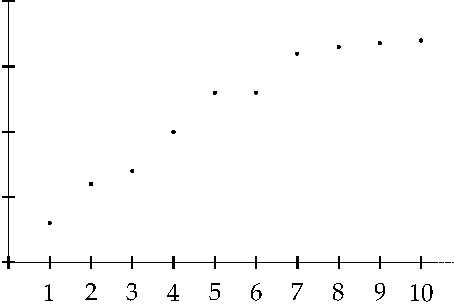
\includegraphics{figures/sequence-increasing}
\caption{First few terms of a monotone increasing sequence as a
graph.\label{figsequenceincreasing}}
\end{myfigureht}

\begin{prop} \label{prop:monotoneconv}
A monotone sequence $\{ x_n \}$ is bounded if and only if it is convergent.

Furthermore, if $\{ x_n \}$ is monotone increasing and bounded, then
\begin{equation*}
\lim_{n\to \infty} x_n = \sup \{ x_n : n \in \N \} .
\end{equation*}
If $\{ x_n \}$ is monotone decreasing and bounded, then
\begin{equation*}
\lim_{n\to \infty} x_n = \inf \{ x_n : n \in \N \} .
\end{equation*}
\end{prop}

\begin{proof}
Let us suppose the sequence is monotone increasing.  Suppose 
the sequence is bounded, so there exists a $B$
such that $x_n \leq B$ for all $n$, that is the set
$\{ x_n : n \in  \N \}$ is bounded above.  Let
\begin{equation*}
x := \sup \{ x_n : n \in \N \} .
\end{equation*}
Let $\epsilon > 0$ be arbitrary.  As $x$ is the supremum, then
there must be at least one $M \in \N$ such that $x_{M} > x-\epsilon$
(because $x$ is the supremum).  As $\{ x_n \}$ is monotone increasing,
then it is easy to see (by \hyperref[induction:thm]{induction}) that
$x_n \geq x_{M}$ for all $n \geq M$.  Hence
\begin{equation*}
\abs{x_n-x} = x-x_n \leq x-x_{M} < \epsilon  .
\end{equation*}
Therefore, the sequence converges to $x$.
We already know that a convergent sequence is bounded, which completes the
other direction of the implication.

The proof for monotone decreasing sequences is left as an exercise.
\end{proof}

\begin{example}
Take the sequence $\bigl\{ \frac{1}{\sqrt{n}} \bigr\}$.

The sequence is
bounded below as
$\frac{1}{\sqrt{n}} > 0$ for all $n \in \N$.
Let us show that it is monotone decreasing.  We start with
$\sqrt{n+1} \geq \sqrt{n}$ (why is that true?).  From this inequality
we obtain
\begin{equation*}
\frac{1}{\sqrt{n+1}} \leq \frac{1}{\sqrt{n}} .
\end{equation*}
So the sequence is monotone decreasing and bounded below (hence
bounded).  We apply the theorem to note that the sequence is
convergent and in fact
\begin{equation*}
\lim_{n\to \infty} \frac{1}{\sqrt{n}}
=
\inf \left\{ \frac{1}{\sqrt{n}} : n \in \N \right\} .
\end{equation*}
We already know that the infimum is greater than or equal to 0, as
0 is a lower bound.  Take a number $b \geq 0$ such
that $b \leq \frac{1}{\sqrt{n}}$ for all $n$.  We square both sides to
obtain
\begin{equation*}
b^2 \leq \frac{1}{n} \qquad \text{for all } n \in \N.
\end{equation*}
We have seen before that this implies that $b^2 \leq 0$ (a consequence
of the \hyperref[thm:arch:i]{Archimedean property}).  As we also have $b^2 \geq 0$, then $b^2 = 0$
and so $b = 0$.
Hence, $b=0$ is the greatest lower bound, and $\lim \frac{1}{\sqrt{n}} = 0$.
\end{example}

\begin{example}
A word of caution:  We must show that a monotone sequence is bounded
in order to use \propref{prop:monotoneconv} to conclude a sequence converges.
The sequence $\{ 1 + \nicefrac{1}{2} + \cdots + \nicefrac{1}{n} \}$
is a monotone increasing
sequence that grows very slowly.  We will see, once we get to series,
that this sequence has no upper bound and so does not converge.  It is not
at all obvious that this sequence has no upper bound.
\end{example}

A common example of where monotone sequences arise is the following
proposition.  The proof is left as an exercise.

\begin{prop} \label{prop:supinfseq}
Let $S \subset \R$ be a nonempty bounded set.
Then there exist monotone sequences
$\{ x_n \}$ and $\{ y_n \}$ such that $x_n, y_n \in S$ and
\begin{equation*}
\sup\,S = \lim_{n\to \infty} x_n \qquad \text{and} \qquad \inf\,S =
\lim_{n\to\infty} y_n .
\end{equation*}
\end{prop}

\subsection{Tail of a sequence}

\begin{defn}
For a sequence $\{ x_n \}$,
the \emph{$K$-tail} (where $K \in \N$)
or just the
\emph{tail}\index{tail of a sequence} of
the sequence is the sequence starting at $K+1$, usually written as
\begin{equation*}
\{ x_{n+K} \}_{n=1}^\infty
\qquad \text{or} \qquad \{ x_n \}_{n=K+1}^\infty .
\end{equation*}
\end{defn}
For example, the $4$-tail of $\{ \nicefrac{1}{n} \}$ is
$\nicefrac{1}{5}, \nicefrac{1}{6}, \nicefrac{1}{7}, \nicefrac{1}{8},
\ldots$.  The $0$-tail of a sequence is the sequence itself.
The convergence and the limit of a sequence only depends on its tail.

\begin{prop}
Let $\{ x_n \}_{n=1}^\infty$ be a sequence.  Then the following
statements are equivalent:
\begin{enumerate}[(i)]
\item \label{prop:ktail:i}
The sequence $\{ x_n \}_{n=1}^\infty$ converges.
\item \label{prop:ktail:ii}
The $K$-tail $\{ x_{n+K} \}_{n=1}^\infty$ converges for all $K \in \N$.
\item \label{prop:ktail:iii}
The $K$-tail $\{ x_{n+K} \}_{n=1}^\infty$ converges for some $K \in \N$.
\end{enumerate}
Furthermore, if any (and hence all) of the limits exist, then for any $K \in \N$
\begin{equation*}
\lim_{n\to \infty} x_n = \lim_{n \to \infty} x_{n+K} .
\end{equation*}
\end{prop}

\begin{proof}
It is clear that
\ref{prop:ktail:ii} implies \ref{prop:ktail:iii}.
We will therefore show first that
\ref{prop:ktail:i}
implies
\ref{prop:ktail:ii},
and then we will show that
\ref{prop:ktail:iii}
implies
\ref{prop:ktail:i}.  That is, 
%mbxSTARTIGNORE
\begin{equation*}
\begin{tikzcd}[row sep=0pt]
& \text{\ref{prop:ktail:ii}} \ar[dr, Rightarrow] & \\
\text{\ref{prop:ktail:i}} \ar[ur, Rightarrow, "\text{to prove}"] & &
\text{\ref{prop:ktail:iii}} \ar[ll, Rightarrow, "\text{to prove}"] 
\end{tikzcd}
\end{equation*}
%mbxENDIGNORE
%mbxlatex \begin{center}
%mbxlatex \subimport*{figures/}{tail_of_sequence_cd.pdf_t}
%mbxlatex \end{center}
In the process we will also show that the limits are equal.

Let us start with \ref{prop:ktail:i} implies \ref{prop:ktail:ii}.
Suppose $\{x_n \}$ converges to some $x \in \R$.
Let $K \in \N$ be arbitrary, and
define $y_n := x_{n+K}$.  We wish to show that $\{ y_n \}$ converges
to $x$.
Given an $\epsilon > 0$, there exists an $M \in \N$ such that
$\abs{x-x_n} < \epsilon$ for all $n \geq M$.
Note that $n \geq M$ implies $n+K \geq M$.  Therefore, for
all $n \geq M$ we have that 
\begin{equation*}
\abs{x-y_n} = \abs{x-x_{n+K}} < \epsilon .
\end{equation*}
Consequently, $\{ y_n \}$ converges to $x$.

Let us move to \ref{prop:ktail:iii} implies \ref{prop:ktail:i}.
Let $K \in \N$ be given, define
$y_n := x_{n+K}$, and suppose that $\{ y_n \}$ converges to $x \in \R$.
That is, given an $\epsilon > 0$, there exists an $M' \in \N$ such that
$\abs{x-y_n} < \epsilon$ for all $n \geq M'$.
Let $M := M'+K$.  Then $n \geq M$ implies $n-K \geq M'$.
Thus, whenever $n \geq M$ we have
\begin{equation*}
\abs{x-x_n} = \abs{x-y_{n-K}} < \epsilon.
\end{equation*}
Therefore $\{ x_n \}$ converges to $x$.
\end{proof}

Essentially, the limit does not care about how the sequence begins, it only
cares about the tail of the sequence.  The beginning of the sequence
may be arbitrary.

For example, the sequence defined by $x_n := \frac{n}{n^2+16}$ is decreasing
if we start at $n=4$ (it is increasing before).  That is:
$\{ x_n \} =
\nicefrac{1}{17},
\nicefrac{1}{10},
\nicefrac{3}{25},
\nicefrac{1}{8},
\nicefrac{5}{41},
\nicefrac{3}{26},
\nicefrac{7}{65},
\nicefrac{1}{10},
\nicefrac{9}{97},
\nicefrac{5}{58},\ldots$, and 
\begin{equation*}
\nicefrac{1}{17} <
\nicefrac{1}{10} <
\nicefrac{3}{25} <
\nicefrac{1}{8} >
\nicefrac{5}{41} >
\nicefrac{3}{26} >
\nicefrac{7}{65} >
\nicefrac{1}{10} >
\nicefrac{9}{97} >
\nicefrac{5}{58} > \ldots .
\end{equation*}
If we throw away the first 3 terms
and look at the 3-tail, it is decreasing.  The proof is left as an exercise.  Since the 3-tail
is monotone and bounded below by zero, it is convergent, and therefore the sequence is convergent.

\subsection{Subsequences}

It is useful to sometimes consider only some terms of a sequence.
A subsequence of $\{ x_n \}$ is a sequence that contains
only some of the numbers from $\{ x_n \}$ in the same order.

\begin{defn}
Let $\{ x_n \}$ be a sequence.
Let $\{ n_i \}$ be a strictly increasing sequence of natural
numbers, that is $n_i < n_{i+1}$ for all $i$ (in other words $n_1 < n_2 < n_3 < \cdots$).  
The sequence
\begin{equation*}
\{ x_{n_i} \}_{i=1}^\infty
\end{equation*}
is called \glsadd{not:subsequence}
a \emph{\myindex{subsequence}} of $\{ x_n \}$.
\end{defn}

Consider the sequence $\{ \nicefrac{1}{n} \}$.  The sequence
$\{ \nicefrac{1}{3n} \}$ is a subsequence.  To see how these two
sequences fit in the definition, take $n_i := 3i$.  
The numbers in the
subsequence must come from the original sequence.  So $1,0,\nicefrac{1}{3},0,
\nicefrac{1}{5},\ldots$
is not a subsequence of $\{ \nicefrac{1}{n} \}$.  Similarly, order
must be preserved.  So
the sequence $1,\nicefrac{1}{3},\nicefrac{1}{2},\nicefrac{1}{5},\ldots$
is not a subsequence of $\{ \nicefrac{1}{n} \}$.

A tail of a sequence is one special type of a subsequence.  For an arbitrary
subsequence, we have the following proposition about convergence.

\begin{prop} \label{prop:seqtosubseq}
If $\{ x_n \}$ is a convergent sequence,
then any subsequence $\{ x_{n_i} \}$ is also convergent and
\begin{equation*}
\lim_{n\to \infty} x_n = 
\lim_{i\to \infty} x_{n_i} .
\end{equation*}
\end{prop}

\begin{proof}
Suppose $\lim_{n\to \infty} x_n = x$.  That means that for every
$\epsilon > 0$ we have an $M \in \N$ such that for all $n \geq M$
\begin{equation*}
\abs{x_n - x} < \epsilon .
\end{equation*}
It is not hard to prove (do it!) by \hyperref[induction:thm]{induction} that
$n_i \geq i$.  Hence $i \geq M$ implies $n_i \geq M$.  Thus,
for all $i \geq M$ we have
\begin{equation*}
\abs{x_{n_i} - x} < \epsilon ,
\end{equation*}
and we are done.
\end{proof}

\begin{example}
Existence of a convergent subsequence does not imply
convergence of the sequence itself.
Take the sequence $0,1,0,1,0,1,\ldots$.  That is,
$x_n = 0$ if $n$ is odd, and $x_n = 1$ if $n$ is even.  The sequence
$\{ x_n \}$ is divergent, however, the subsequence
$\{ x_{2n} \}$ converges to 1 and the subsequence
$\{ x_{2n+1} \}$ converges to 0.  Compare \propref{seqconvsubseqconv:prop}.
\end{example}

\subsection{Exercises}

\begin{exnote}
In the following exercises, feel free to use what you know from calculus to
find the limit, if it exists.  But you must \emph{prove}
that you
found the correct limit, or prove that the series is divergent.
\end{exnote}

\begin{exercise}
Is the sequence
$\{ 3n \}$
bounded?  Prove or disprove.
\end{exercise}

\begin{exercise}
Is the sequence
$\{ n \}$
convergent?  If so, what is the limit?
\end{exercise}

\begin{exercise}
Is the sequence
$\left\{ \dfrac{{(-1)}^n}{2n} \right\}$
convergent?  If so, what is the limit?
\end{exercise}

\begin{exercise}
Is the sequence
$\{ 2^{-n} \}$
convergent?  If so, what is the limit?
\end{exercise}

\begin{exercise}
Is the sequence
$\left\{ \dfrac{n}{n+1} \right\}$
convergent?  If so, what is the limit?
\end{exercise}

\begin{exercise}
Is the sequence
$\left\{ \dfrac{n}{n^2+1} \right\}$
convergent?  If so, what is the limit?
\end{exercise}

\begin{exercise} \label{exercise:absconv}
Let $\{ x_n \}$ be a sequence.
\begin{enumerate}[a)]
\item Show that $\lim\, x_n = 0$ (that is, the limit exists and is zero)
if and only if $\lim \abs{x_n} = 0$.
\item Find an example such that $\{ \abs{x_n} \}$ converges and $\{ x_n \}$
diverges.
\end{enumerate}
\end{exercise}

\begin{exercise}
Is the sequence
$\left\{ \dfrac{2^n}{n!} \right\}$
convergent?  If so, what is the limit?
\end{exercise}

\begin{exercise}
Show that the sequence
$\left\{ \dfrac{1}{\sqrt[3]{n}} \right\}$ is monotone and bounded.  Then use
\propref{prop:monotoneconv} to find the limit.
\end{exercise}

\begin{exercise}
Show that the sequence
$\left\{ \dfrac{n+1}{n} \right\}$
is monotone and bounded.  Then use
\propref{prop:monotoneconv} to find the limit.
\end{exercise}

\begin{exercise}
Finish the proof of \propref{prop:monotoneconv} for monotone decreasing
sequences.
\end{exercise}

\begin{exercise}
Prove \propref{prop:supinfseq}.
\end{exercise}

\begin{exercise}
Let $\{ x_n \}$ be a convergent monotone sequence.  Suppose 
there exists a $k \in \N$ such that
\begin{equation*}
\lim_{n\to \infty} x_n = x_k .
\end{equation*}
Show that $x_n = x_k$ for all $n \geq k$.
\end{exercise}

\begin{exercise}
Find a convergent subsequence of the sequence
$\{ {(-1)}^n \}$.
\end{exercise}

\begin{exercise}
Let $\{x_n\}$ be a sequence defined by
\begin{equation*}
x_n := 
\begin{cases}
n               & \text{if } n \text{ is odd} , \\
\nicefrac{1}{n} & \text{if } n \text{ is even} .
\end{cases}
\end{equation*}
\begin{enumerate}[a)]
\item Is the sequence bounded? (prove or disprove)
\item Is there a convergent subsequence?  If so, find it.
\end{enumerate}
\end{exercise}

\begin{exercise}
Let $\{ x_n \}$ be a sequence.
Suppose there are two convergent subsequences $\{ x_{n_i} \}$ and
$\{ x_{m_i} \}$.  Suppose 
\begin{equation*}
\lim_{i\to\infty} x_{n_i} = a
\qquad \text{and} \qquad
\lim_{i\to\infty} x_{m_i} = b,
\end{equation*}
where $a \not= b$.  Prove that $\{ x_n \}$ is not convergent, without
using \propref{prop:seqtosubseq}.
\end{exercise}

\begin{exercise}[Tricky]
Find a sequence $\{ x_n \}$ such that for any $y \in \R$, there exists a
subsequence $\{ x_{n_i} \}$ converging to $y$.
\end{exercise}

\begin{exercise}[Easy]
Let $\{ x_n \}$ be a sequence and $x \in \R$.
Suppose for any $\epsilon > 0$, there is an $M$ such that for
all $n \geq M$, $\abs{x_n-x} \leq \epsilon$.  Show that $\lim\, x_n = x$.
\end{exercise}

\begin{exercise}[Easy]
Let $\{ x_n \}$ be a sequence and $x \in \R$ such that
there exists a $k \in \N$ such that for all $n \geq k$,
$x_n = x$.  Prove that $\{ x_n \}$ converges to $x$.
\end{exercise}

\begin{exercise}
Let $\{ x_n \}$ be a sequence and
define a sequence $\{ y_n \}$ by
$y_{2k} := x_{k^2}$ and $y_{2k-1} := x_k$ for all $k \in \N$.
Prove that $\{ x_n \}$ converges if and only if $\{ y_n \}$ converges.
Furthermore, prove that if they converge, then
$\lim\, x_n = \lim\, y_n$.
\end{exercise}

\begin{exercise}
Show that the 3-tail of the sequence defined by $x_n := \frac{n}{n^2+16}$ is
monotone decreasing.  Hint: Suppose $n \geq m \geq 4$ and consider the 
numerator of the expression $x_n-x_m$.
\end{exercise}

\begin{exercise}
Suppose that $\{ x_n \}$ is a sequence such that
the subsequences $\{ x_{2n} \}$, $\{ x_{2n-1} \}$, and
$\{ x_{3n} \}$ all converge.  Show that $\{ x_n \}$ is convergent.
\end{exercise}


%%%%%%%%%%%%%%%%%%%%%%%%%%%%%%%%%%%%%%%%%%%%%%%%%%%%%%%%%%%%%%%%%%%%%%%%%%%%%%

\sectionnewpage
\section{Facts about limits of sequences}
\label{sec:factslimsseqs}

\sectionnotes{2--2.5 lectures, recursively defined sequences can safely be
skipped}

In this section we go over some basic results about the limits of
sequences.
We start by looking at how sequences interact with inequalities.

\subsection{Limits and inequalities}

A basic lemma about limits and inequalities is the so-called squeeze lemma.
It allows us to show convergence of sequences in difficult cases
if we find two other simpler convergent sequences that 
\myquote{squeeze} the original sequence.

\begin{lemma}[Squeeze lemma]\index{squeeze lemma} \label{squeeze:lemma}
Let $\{ a_n \}$, 
$\{ b_n \}$, and 
$\{ x_n \}$ be sequences such that
\begin{equation*}
a_n \leq x_n \leq b_n \quad \text{for all } n \in \N.
\end{equation*}
Suppose $\{ a_n \}$ and $\{ b_n \}$ converge and
\begin{equation*}
\lim_{n\to \infty} a_n
=
\lim_{n\to \infty} b_n .
\end{equation*}
Then $\{ x_n \}$ converges and
\begin{equation*}
\lim_{n\to \infty} x_n
=
\lim_{n\to \infty} a_n
=
\lim_{n\to \infty} b_n .
\end{equation*}
\end{lemma}

\begin{proof}
Let $x := \lim\, a_n = \lim\, b_n$.
Let $\epsilon > 0$ be given.
Find an $M_1$ such that for all $n \geq M_1$ we have
that $\abs{a_n-x} < \epsilon$, and an $M_2$
such that for all $n \geq M_2$
we have $\abs{b_n-x} < \epsilon$.  Set $M := \max \{M_1, M_2 \}$.
Suppose $n \geq M$.
In particular, we have
$x - a_n < \epsilon$ or 
$x - \epsilon < a_n$.  Similarly we have that $b_n < x + \epsilon$.
Putting everything together, we find
\begin{equation*}
x - \epsilon < a_n \leq x_n \leq b_n < x + \epsilon .
\end{equation*}
In other words, $-\epsilon < x_n-x < \epsilon$ or $\abs{x_n-x} < \epsilon$.
So $\{x_n\}$ converges to $x$.
See \figureref{figsqueeze}.
\end{proof}

\begin{myfigureht}
\subimport*{figures/}{figsqueeze.pdf_t}
\caption{Squeeze lemma proof in picture.\label{figsqueeze}}
\end{myfigureht}

\begin{example}
One application of
the \hyperref[squeeze:lemma]{squeeze lemma} is to compute limits of 
sequences using limits that we already know.  For example, consider
the sequence $\{ \frac{1}{n\sqrt{n}} \}$.
Since $\sqrt{n} \geq 1$ for all $n \in \N$, we have
\begin{equation*}
0 \leq \frac{1}{n\sqrt{n}} \leq \frac{1}{n}
\end{equation*}
for all $n \in \N$.  We already know $\lim \nicefrac{1}{n} = 0$. 
Hence, using
the constant sequence $\{ 0 \}$ and the sequence $\{ \nicefrac{1}{n} \}$ in the
squeeze lemma, we conclude
\begin{equation*}
\lim_{n\to\infty} \frac{1}{n\sqrt{n}} = 0 .
\end{equation*}
\end{example}

Limits also preserve inequalities.

\begin{lemma} \label{limandineq:lemma}
Let $\{ x_n \}$ and $\{ y_n \}$ be
convergent sequences and
\begin{equation*}
x_n \leq y_n ,
\end{equation*}
for all $n \in \N$.  Then
\begin{equation*}
\lim_{n\to\infty} x_n \leq
\lim_{n\to\infty} y_n .
\end{equation*}
\end{lemma}

\begin{proof}
Let $x := \lim\, x_n$ and $y := \lim\, y_n$. 
Let 
$\epsilon > 0$ be given.  Find an $M_1$ such that for all $n \geq M_1$
we have $\abs{x_n-x} < \nicefrac{\epsilon}{2}$.  Find an $M_2$ such that
for all $n \geq M_2$ we have
$\abs{y_n-y} < \nicefrac{\epsilon}{2}$.  In particular,
for some $n \geq \max\{ M_1, M_2 \}$ we have
$x-x_n < \nicefrac{\epsilon}{2}$ and
$y_n-y < \nicefrac{\epsilon}{2}$.  We add these inequalities to
obtain
\begin{equation*}
y_n-x_n+x-y < \epsilon, \qquad \text{or} \qquad
y_n-x_n < y-x+ \epsilon .
\end{equation*}
Since $x_n \leq y_n$ we have
$0 \leq y_n-x_n$ and hence $0 < y-x+ \epsilon$.
In other words,
\begin{equation*}
x-y < \epsilon .
\end{equation*}
Because $\epsilon > 0$ was arbitrary, we obtain
$x-y \leq 0$.
Therefore, $x \leq y$.
\end{proof}

The following corollary is
proved
using constant sequences in
\lemmaref{limandineq:lemma}.  The proof is left as an exercise.

\begin{samepage}
\begin{cor} \label{limandineq:cor}
\leavevmode
\begin{enumerate}[(i)]
\item Let $\{ x_n \}$ be a convergent sequence such that $x_n \geq 0$,
then
\begin{equation*}
\lim_{n\to\infty} x_n \geq 0.
\end{equation*}
\item
Let $a,b \in \R$ and
let $\{ x_n \}$ be a convergent sequence such that
\begin{equation*}
a \leq x_n \leq b ,
\end{equation*}
for all $n \in \N$.  Then
\begin{equation*}
a \leq \lim_{n\to\infty} x_n \leq b.
\end{equation*}
\end{enumerate}
\end{cor}
\end{samepage}

In \lemmaref{limandineq:lemma} and \corref{limandineq:cor} we cannot simply replace
all the non-strict inequalities with
strict inequalities.  For example,
let $x_n := \nicefrac{-1}{n}$ and $y_n := \nicefrac{1}{n}$.
Then $x_n < y_n$, $x_n < 0$,
and $y_n > 0$ for all $n$.  However, these inequalities are
not preserved by the limit operation as we have
$\lim\, x_n = \lim\, y_n = 0$.
The moral of this example is that strict inequalities may become non-strict
inequalities when limits are applied; if we know
$x_n < y_n$ for all $n$,
we may only conclude 
\begin{equation*}
\lim_{n \to \infty} x_n \leq
\lim_{n \to \infty} y_n .
\end{equation*}
This issue is a common source of errors.

\subsection{Continuity of algebraic operations}

Limits interact nicely with algebraic operations.

\begin{prop} \label{prop:contalg}
Let $\{ x_n \}$ and $\{ y_n \}$ be convergent sequences.
\begin{enumerate}[(i)]
\item \label{prop:contalg:i}
The sequence $\{ z_n \}$, where $z_n := x_n + y_n$, converges and
\begin{equation*}
\lim_{n \to \infty} (x_n + y_n) = 
\lim_{n \to \infty} z_n = 
\lim_{n \to \infty} x_n + 
\lim_{n \to \infty} y_n .
\end{equation*}
\item \label{prop:contalg:ii}
The sequence $\{ z_n \}$, where $z_n := x_n - y_n$, converges and
\begin{equation*}
\lim_{n \to \infty} (x_n - y_n) = 
\lim_{n \to \infty} z_n = 
\lim_{n \to \infty} x_n - 
\lim_{n \to \infty} y_n .
\end{equation*}
\item \label{prop:contalg:iii}
The sequence $\{ z_n \}$, where $z_n := x_n y_n$, converges and
\begin{equation*}
\lim_{n \to \infty} (x_n y_n) = 
\lim_{n \to \infty} z_n = 
\left( \lim_{n \to \infty} x_n \right)
\left( \lim_{n \to \infty} y_n \right) .
\end{equation*}
\item \label{prop:contalg:iv}
If $\lim\, y_n \not= 0$ and $y_n \not= 0$ for all $n \in \N$, then
the sequence $\{ z_n \}$, where $z_n := \dfrac{x_n}{y_n}$, converges and
\begin{equation*}
\lim_{n \to \infty} \frac{x_n}{y_n} = 
\lim_{n \to \infty} z_n = 
%\frac{\lim_{n \to \infty} x_n}{\lim_{n \to \infty} y_n} .
\frac{\lim\, x_n}{\lim\, y_n} .
\end{equation*}
\end{enumerate}
\end{prop}

\begin{proof}
Let us start with \ref{prop:contalg:i}.
Suppose $\{ x_n \}$ and $\{ y_n \}$ are convergent sequences and
write $z_n := x_n + y_n$.  Let $x := \lim\, x_n$,
$y := \lim\, y_n$, and $z := x+y$.

Let $\epsilon > 0$ be given.  
Find an $M_1$ such that for all $n \geq M_1$
we have
$\abs{x_n - x} < \nicefrac{\epsilon}{2}$.  
Find an $M_2$ such that for all $n \geq M_2$
we have
$\abs{y_n - y} < \nicefrac{\epsilon}{2}$.  Take $M := \max \{ M_1, M_2 \}$.
For all $n \geq M$ we have
\begin{equation*}
\begin{split}
\abs{z_n - z} &=
\abs{(x_n+y_n) - (x+y)} \\
& =
\abs{x_n-x + y_n-y} \\
& \leq
\abs{x_n-x} + \abs{y_n-y} \\
& <
\frac{\epsilon}{2} +
\frac{\epsilon}{2}
= \epsilon.
\end{split}
\end{equation*}
Therefore \ref{prop:contalg:i} is proved.
Proof of \ref{prop:contalg:ii} is almost identical and is left as an
exercise.

Let us tackle 
\ref{prop:contalg:iii}.
Suppose again that $\{ x_n \}$ and $\{ y_n \}$ are convergent sequences and
write $z_n := x_n y_n$.  Let $x := \lim\, x_n$,
$y := \lim\, y_n$, and $z := xy$.

Let $\epsilon > 0$ be given.
Let $K := \max\{ \abs{x}, \abs{y}, \nicefrac{\epsilon}{3} , 1 \}$.
Find an $M_1$ such that for all $n \geq M_1$
we have
$\abs{x_n - x} < \frac{\epsilon}{3K}$.
Find an $M_2$ such that for all $n \geq M_2$
we have
$\abs{y_n - y} < \frac{\epsilon}{3K}$.  Take $M := \max \{ M_1, M_2 \}$.
For all $n \geq M$ we have
\begin{equation*}
\begin{split}
\abs{z_n - z} &=
\abs{(x_ny_n) - (xy)} \\
& =
\abs{(x_n-x+x)(y_n-y+y) - xy} \\
& =
\abs{(x_n-x)y + x(y_n-y) +(x_n-x)(y_n-y)} \\
& \leq
\abs{(x_n-x)y} + \abs{x(y_n - y)} +
\abs{(x_n-x)(y_n-y)} \\
& =
\abs{x_n -x}\abs{y} + 
\abs{x}\abs{y_n -y} + 
\abs{x_n -x}\abs{y_n -y}
\\
& <
\frac{\epsilon}{3K} K + 
K \frac{\epsilon}{3K} + 
\frac{\epsilon}{3K}
\frac{\epsilon}{3K}
\qquad \qquad \text{(now notice that } \tfrac{\epsilon}{3K} \leq 1
\text{ and }
K \geq 1\text{)}
\\
& \leq
\frac{\epsilon}{3} + \frac{\epsilon}{3} + \frac{\epsilon}{3}
 = \epsilon .
\end{split}
\end{equation*}

Finally, let us tackle
\ref{prop:contalg:iv}.  Instead of proving 
\ref{prop:contalg:iv} directly, we prove the following simpler claim:

Claim: \emph{If $\{ y_n \}$ is a convergent sequence such that
$\lim\, y_n \not= 0$ and $y_n \not= 0$ for all $n \in \N$, then
$\{ \nicefrac{1}{y_n} \}$ converges and}
\begin{equation*}
\lim_{n\to\infty} \frac{1}{y_n} = \frac{1}{\lim\, y_n}  .
\end{equation*}

Once the claim is proved, we take the sequence $\{ \nicefrac{1}{y_n} \}$,
multiply it by the sequence $\{ x_n \}$ and apply item
\ref{prop:contalg:iii}.

Proof of claim:  Let $\epsilon > 0$ be given.
Let $y := \lim\, y_n$.
As $\abs{y} \not= 0$, then
$\min \left\{ \abs{y}^2\frac{\epsilon}{2}, \, \frac{\abs{y}}{2} \right\} > 0$.
Find an $M$ such that for all $n \geq M$
we have
\begin{equation*}
\abs{y_n - y} < \min \left\{ \abs{y}^2\frac{\epsilon}{2}, \, \frac{\abs{y}}{2}
\right\} .
\end{equation*}
For all $n \geq M$ we have
$\abs{y - y_n} < \frac{\abs{y}}{2}$, and so
\begin{equation*}
\abs{y} = 
\abs{y - y_n + y_n } \leq
\abs{y - y_n} + \abs{ y_n } < \frac{\abs{y}}{2} + \abs{y_n}.
\end{equation*}
Subtracting $\nicefrac{\abs{y}}{2}$ from both sides we obtain
$\nicefrac{\abs{y}}{2} < \abs{y_n}$, or in other words,
\begin{equation*}
\frac{1}{\abs{y_n}} < \frac{2}{\abs{y}} .
\end{equation*}
We finish the proof of the claim:
\begin{equation*}
\begin{split}
\abs{\frac{1}{y_n} - \frac{1}{y}} &=
\abs{\frac{y - y_n}{y y_n}} \\
& =
\frac{\abs{y - y_n}}{\abs{y} \abs{y_n}} \\
& \leq
\frac{\abs{y - y_n}}{\abs{y}} \, \frac{2}{\abs{y}} \\
& <
\frac{\abs{y}^2 \frac{\epsilon}{2}}{\abs{y}} \, \frac{2}{\abs{y}}
= \epsilon .
\end{split}
\end{equation*}
And we are done.
\end{proof}

By plugging in constant sequences, we get several easy corollaries.
If $c \in \R$ and $\{ x_n \}$ is a convergent sequence, then
for example
\begin{equation*}
\lim_{n \to \infty} c x_n = 
c \left( \lim_{n \to \infty} x_n \right) \qquad
\text{and}
\qquad
\lim_{n \to \infty} (c + x_n) = 
c + \lim_{n \to \infty} x_n .
\end{equation*}
Similarly, we find such equalities for constant subtraction and division.

As we can take limits past multiplication we can show (exercise)
that $\lim\, x_n^k = {(\lim\, x_n)}^k$ for all $k \in \N$.
That is, we can take limits
past powers.  Let us see if we can do the same with roots.

\begin{prop}
Let $\{ x_n \}$ be a convergent sequence such
that $x_n \geq 0$.
Then
\begin{equation*}
\lim_{n\to\infty} \sqrt{x_n} =
\sqrt{ \lim_{n\to\infty} x_n } .
\end{equation*}
\end{prop}

Of course to even make this statement, we need to apply
\corref{limandineq:cor} to show
that
$\lim\, x_n \geq 0$, so that we can take the square root without
worry.

\begin{proof}
Let $\{ x_n \}$ be a convergent sequence and let $x := \lim\, x_n$.
As we just mentioned, $x \geq 0$.

First suppose $x=0$.  Let $\epsilon > 0$ be given.
Then there is an $M$ such that for all $n \geq M$ we have
$x_n = \abs{x_n} < \epsilon^2$, or in other words $\sqrt{x_n} < \epsilon$.
Hence
\begin{equation*}
\abs{\sqrt{x_n} - \sqrt{x}} =
\sqrt{x_n} < \epsilon.
\end{equation*}

Now suppose $x > 0$ (and hence $\sqrt{x} > 0$).
\begin{equation*}
\begin{split}
\abs{\sqrt{x_n}-\sqrt{x}} &= 
\abs{\frac{x_n-x}{\sqrt{x_n}+\sqrt{x}}} \\
&=
\frac{1}{\sqrt{x_n}+\sqrt{x}}
\abs{x_n-x} \\
& \leq
\frac{1}{\sqrt{x}}
\abs{x_n-x} .
\end{split}
\end{equation*}
We leave the rest of the proof to the reader.
\end{proof}

A similar proof works for the $k$th root.  That is, we also
obtain
$\lim\, x_n^{1/k} = {( \lim\, x_n )}^{1/k}$.  We leave this to the reader
as a challenging exercise.

We may also want to take the limit past the absolute value sign.
The converse of this proposition is not true, see
\exerciseref{exercise:absconv} part b).

\begin{prop}
If $\{ x_n \}$ is a convergent sequence, then $\{ \abs{x_n} \}$
is convergent and
\begin{equation*}
\lim_{n\to\infty} \abs{x_n} = 
\abs{\lim_{n\to\infty} x_n} .
\end{equation*}
\end{prop}

\begin{proof}
We simply note the reverse triangle inequality
\begin{equation*}
\big\lvert \abs{x_n} - \abs{x} \big\rvert \leq \abs{x_n-x} .
\end{equation*}
Hence if $\abs{x_n -x}$ can be made arbitrarily small, so can
$\big\lvert \abs{x_n} - \abs{x} \big\rvert$.
Details are left to the reader.
\end{proof}

Let us see an example putting the propositions above together.  Since
$\lim \nicefrac{1}{n} = 0$, then
\begin{equation*}
\lim_{n\to \infty}
\abs{\sqrt{1 + \nicefrac{1}{n}} - \nicefrac{100}{n^2}} =  
\abs{\sqrt{1 + (\lim \nicefrac{1}{n})} - 100 (\lim \nicefrac{1}{n})(\lim
\nicefrac{1}{n})} = 1.
\end{equation*}
That is, the limit on the left hand side exists because the right hand
side exists.  You really should read the equality above from right to left.

On the other hand you must apply the propositions carefully.
For example, by rewriting the expression with common denominator first
we find
\begin{equation*}
\lim_{n\to \infty} \left( \frac{n^2}{n+1} - n \right)
= -1 .
\end{equation*}
However, 
$\bigl\{ \frac{n^2}{n+1} \bigr\}$ and 
$\{n\}$ are not convergent,
so
$\bigl(\lim\, \frac{n^2}{n+1}\bigr) -
\bigl(\lim\, n\bigr)$ is nonsense.

\subsection{Recursively defined sequences}

Now that we know we can interchange limits and algebraic operations, we can
compute the limits of many sequences.
One such class are recursively defined sequences, that is, sequences where
the next number in the sequence is computed using a formula from a fixed number
of preceding elements in the sequence.

\begin{example}
Let $\{ x_n \}$ be defined by $x_1 := 2$ and
\begin{equation*}
x_{n+1} := x_n - \frac{x_n^2-2}{2x_n} .
\end{equation*}
We must first find out if this sequence is well-defined; we must show we never
divide by zero.
Then we must find out if the sequence converges.  Only then
can we attempt to find the limit.

So let us prove 
$x_n$ exists and $x_n > 0$ for all $n$ (so the sequence is well-defined
and bounded below).
Let us show this by \hyperref[induction:thm]{induction}.  We know that
$x_1 = 2 > 0$.  For the induction step, suppose $x_n > 0$.  Then
\begin{equation*}
x_{n+1} = x_n - \frac{x_n^2-2}{2x_n} =
\frac{2x_n^2 - x_n^2+2}{2x_n} =
\frac{x_n^2+2}{2x_n} .
\end{equation*}
It is always true that $x_n^2+2 > 0$,
and as
$x_n > 0$, then $\frac{x_n^2+2}{2x_n} > 0$ and hence $x_{n+1} > 0$.

Next let us
show that the sequence is monotone decreasing.  If we show that
$x_n^2-2 \geq 0$ for all $n$, then $x_{n+1} \leq x_n$ for all $n$.
Obviously $x_1^2-2 = 4-2 = 2 > 0$.  For an arbitrary $n$ we have 
\begin{equation*}
x_{n+1}^2-2 =
{\left( \frac{x_n^2+2}{2x_n} \right)}^2 - 2
=
\frac{x_n^4+4x_n^2+4 - 8x_n^2}{4x_n^2}
=
\frac{x_n^4-4x_n^2+4}{4x_n^2}
=
\frac{{\left( x_n^2-2 \right)}^2}{4x_n^2} .
\end{equation*}
Since any square is nonnegative,
$x_{n+1}^2-2 \geq 0$ for all $n$.  Therefore,
$\{ x_n \}$ is monotone decreasing and bounded ($x_n > 0$ for all $n$), and 
so the limit exists.  It remains to find the limit.

Write
\begin{equation*}
2x_nx_{n+1} = x_n^2+2 .
\end{equation*}
Since $\{ x_{n+1} \}$ is the 1-tail of $\{ x_n \}$, it converges to the
same limit.  Let us define $x := \lim\, x_n$.  Take the limit of
both sides to obtain
\begin{equation*}
2x^2 = x^2+2 ,
\end{equation*}
or $x^2 = 2$.  As $x_n > 0$ for all $n$ we get $x \geq 0$, and therefore $x = \sqrt{2}$.
\end{example}

You may have seen the sequence above before.  It is
\emph{Newton's method}%
\footnote{%
Named after the English physicist and mathematician
\href{https://en.wikipedia.org/wiki/Isaac_Newton}{Isaac Newton}
(1642--1726/7).}
for finding the square root of 2.  This method comes up often in
practice and converges very rapidly.  We used the fact that
$x_1^2 -2 >0$, although it was not strictly needed to show convergence by
considering a tail of the sequence.
The sequence converges as long as $x_1 \not= 0$, although with a negative $x_1$
we would arrive at $x=-\sqrt{2}$.  By replacing the 2 in the numerator we 
obtain the square root of any positive number.  These statements are left as
an exercise.

You should, however, be careful.  Before taking any limits, you must
make sure the sequence converges.  Let us see an example.

\begin{example}
Suppose $x_1 := 1$ and $x_{n+1} := x_n^2+x_n$.
If we blindly assumed that the limit exists (call it $x$), then we
would get the equation $x = x^2+x$, from which we might
conclude $x=0$.  However, it is not hard
to show that $\{ x_n \}$ is unbounded and therefore does not converge.

The thing to notice in this example is that the method still works, but
it depends on the initial value $x_1$.  If we set $x_1 := 0$,
then the sequence converges and the limit really is 0.
An entire branch of mathematics, called dynamics, deals precisely with these
issues.
See
\exerciseref{exercise:convergentinitialvalues}.
\end{example}

\subsection{Some convergence tests}

It is not always necessary to go back to the definition of convergence
to prove that a sequence is convergent.  We first give a simple convergence test.
The main idea is that 
$\{ x_n \}$ converges to $x$ if and only if 
$\{ \abs{ x_n - x } \}$ converges to zero.

\begin{prop} \label{convzero:prop}
Let $\{ x_n \}$ be a sequence. 
Suppose there is an $x \in \R$
and a convergent sequence $\{ a_n \}$
such that
\begin{equation*}
\lim_{n\to\infty} a_n = 0
\end{equation*}
and 
\begin{equation*}
\abs{x_n - x} \leq a_n
\end{equation*}
for all $n$.  Then $\{ x_n \}$ converges and $\lim\, x_n = x$.
\end{prop}

\begin{proof}
Let $\epsilon > 0$ be given.  Note that $a_n \geq 0$
for all $n$.  Find an $M \in \N$ such that for
all $n \geq M$ we have
$a_n = \abs{a_n - 0} < \epsilon$.  Then, for all $n \geq M$
we have
\begin{equation*}
\abs{x_n - x} \leq a_n < \epsilon . \qedhere
\end{equation*}
\end{proof}

As the proposition shows, to study when a sequence has a limit is 
the same as studying when another sequence goes to zero.
In general, it may be hard to decide if a sequence converges, but
for certain sequences there exist easy to apply tests that tell us
if the sequence converges or not.  Let us see one such test.
First, let
us compute the limit of a certain specific sequence.
\begin{prop}
Let $c > 0$.
\begin{enumerate}[(i)]
\item
If $c < 1$, then
\begin{equation*}
\lim_{n\to\infty} c^n = 0.
\end{equation*}
\item
If $c > 1$, then $\{ c^n \}$ is unbounded.
\end{enumerate}
\end{prop}

\begin{proof}
First suppose $c < 1$.  As $c > 0$, then $c^n > 0$ for all $n \in \N$ by
\hyperref[induction:thm]{induction}.  As $c < 1$, then $c^{n+1} < c^n$ for all $n$.  So we have
a decreasing sequence that is bounded below.  Hence, it is convergent.
Let $L := \lim\, c^n$.  The 1-tail $\{ c^{n+1} \}$
also converges to $L$.  Taking the limit of both sides of $c^{n+1} = c \cdot
c^n$, we obtain $L = cL$, or $(1-c)L=0$.  It follows that $L=0$ as $c \not= 1$.

Now suppose $c > 1$. Suppose for contradiction that the sequence is bounded above by $B > 0$, that is,
$c^n \leq B$ for all $n \in \N$.  Then for all $n$,
\begin{equation*}
{\left(\frac{1}{c}\right)}^n = \frac{1}{c^n} \geq \frac{1}{B} > 0 .
\end{equation*}
As $\nicefrac{1}{c} < 1$, then $\{ {(\nicefrac{1}{c})}^n \}$
converges to 0, contradicts the bound above.
\end{proof}

In the proposition above, the
ratio of the $(n+1)$th term and the $n$th term is $c$.  We 
generalize this simple result to a larger class of sequences.
The following lemma will come up again once we get to series.

\begin{lemma}[Ratio test for sequences]\index{ratio test for sequences}
\label{seq:ratiotest}
Let $\{ x_n \}$ be a sequence such that $x_n \not= 0$ for all $n$ and such that
the limit
\begin{equation*}
L := \lim_{n\to\infty} \frac{\abs{x_{n+1}}}{\abs{x_n}}
\qquad
\text{exists.}
\end{equation*}
\begin{enumerate}[(i)]
\item
If $L < 1$, then $\{ x_n \}$ converges and $\lim\, x_n = 0$.
\item
If $L > 1$, then $\{ x_n \}$ is unbounded (hence diverges).
\end{enumerate}
\end{lemma}

If $L$ exists, but $L=1$, the lemma says nothing.  We cannot make any
conclusion based on that information alone.  For example,
the sequence $\{ \nicefrac{1}{n} \}$ converges to zero, but $L=1$.
The constant sequence $\{ 1 \}$ converges to 1, not zero, and 
$L=1$.  The sequence $\{ {(-1)}^n \}$ does not converge at all, and $L=1$ as
well.
Finally, the sequence $\{  n \}$ is unbounded, yet again $L=1$.
The statement may be strengthened, see 
exercises \ref{exercise:strongerratiotest1} and
\ref{exercise:strongerratiotest2}.

\begin{proof}
Suppose $L < 1$.
As
$\frac{\abs{x_{n+1}}}{\abs{x_n}} \geq 0$ for all $n$, then $L \geq 0$.  Pick
$r$ such that $L < r < 1$.
We wish to compare the sequence $\{ x_n \}$ to the sequence $\{ r^n \}$.  The idea is that
while the ratio $\frac{\abs{x_{n+1}}}{\abs{x_n}}$ is not going to be less than $L$ eventually,
it will eventually be less than $r$, which is still less than 1.
The intuitive idea of the proof is illustrated in \figureref{figratseq}.
\begin{myfigureht}
\subimport*{figures/}{figratseq.pdf_t}
\caption{Proof of ratio test in picture.  The short lines represent the
ratios 
$\frac{\abs{x_{n+1}}}{\abs{x_n}}$
approaching $L$.\label{figratseq}}
\end{myfigureht}

As $r-L > 0$, there exists an $M \in \N$ such that for
all $n \geq M$ we have
\begin{equation*}
\abs{\frac{\abs{x_{n+1}}}{\abs{x_n}} - L} < r-L 
\end{equation*}
Therefore, for $n \geq M$,
\begin{equation*}
\frac{\abs{x_{n+1}}}{\abs{x_n}} - L < r-L 
\qquad \text{or} \qquad
\frac{\abs{x_{n+1}}}{\abs{x_n}} < r .
\end{equation*}
For $n > M$ (that is for $n \geq M+1$)
write
\begin{equation*}
\abs{x_n} =
\abs{x_M}
\frac{\abs{x_{M+1}}}{\abs{x_{M}}}
\frac{\abs{x_{M+2}}}{\abs{x_{M+1}}}
\cdots
\frac{\abs{x_{n}}}{\abs{x_{n-1}}}
<
\abs{x_M}
r r \cdots r = \abs{x_M} r^{n-M} = (\abs{x_M} r^{-M}) r^n .
\end{equation*}
The sequence $\{ r^n \}$ converges to zero and hence 
$\abs{x_M} r^{-M} r^n$ converges to zero.  By \propref{convzero:prop},
the $M$-tail of 
$\{x_n\}$ converges to zero and therefore $\{x_n\}$ converges to zero.

Now suppose $L > 1$.  Pick
$r$ such that $1 < r < L$.  As $L-r > 0$,
there exists an $M \in \N$ such that for
all $n \geq M$
\begin{equation*}
\abs{\frac{\abs{x_{n+1}}}{\abs{x_n}} - L} < L-r .
\end{equation*}
Therefore,
\begin{equation*}
\frac{\abs{x_{n+1}}}{\abs{x_n}} > r .
\end{equation*}
Again for $n > M$,
write
\begin{equation*}
\abs{x_n} =
\abs{x_M}
\frac{\abs{x_{M+1}}}{\abs{x_{M}}}
\frac{\abs{x_{M+2}}}{\abs{x_{M+1}}}
\cdots
\frac{\abs{x_{n}}}{\abs{x_{n-1}}}
>
\abs{x_M}
r r \cdots r = \abs{x_M} r^{n-M} = (\abs{x_M} r^{-M}) r^n .
\end{equation*}
The sequence $\{ r^n \}$ is unbounded (since $r > 1$), and therefore
$\{x_n\}$ cannot be bounded (if $\abs{x_n} \leq B$ for all $n$, then
$r^n < \frac{B}{\abs{x_M}} r^{\:M}$ for all $n$, which is impossible).
Consequently, $\{ x_n \}$ cannot converge.
\end{proof}

\begin{example}
A simple application of the lemma above is to prove 
\begin{equation*}
\lim_{n\to\infty} \frac{2^n}{n!} = 0 .
\end{equation*}

Proof:
Compute
\begin{equation*}
\frac{2^{n+1} / (n+1)!}{2^n/n!}
=
\frac{2^{n+1}}{2^n}\frac{n!}{(n+1)!}
=
\frac{2}{n+1} .
\end{equation*}
It is not hard to see that $\{ \frac{2}{n+1} \}$ converges to zero.
The conclusion follows by the lemma.
\end{example}

\begin{example} \label{example:nto1overn}
A more complicated (and useful) application of the ratio test is to prove 
\begin{equation*}
\lim_{n\to\infty} n^{1/n} = 1 .
\end{equation*}

Proof:
Let $\epsilon > 0$ be given.  Consider the sequence
$\bigl\{ \frac{n}{{(1+\epsilon)}^n} \bigr\}$.  Compute
\begin{equation*}
\frac{(n+1)/{(1+\epsilon)}^{n+1}}{n/{(1+\epsilon)}^{n}}
=
\frac{n+1}{n} \frac{1}{1+\epsilon} .
\end{equation*}
The limit of $\frac{n+1}{n} = 1+\frac{1}{n}$ as $n \to \infty$ is 1, and so
\begin{equation*}
\lim_{n\to \infty} \frac{(n+1)/{(1+\epsilon)}^{n+1}}{n/{(1+\epsilon)}^{n}}
=
\frac{1}{1+\epsilon}  < 1 .
\end{equation*}
Therefore, $\bigl \{ \frac{n}{{(1+\epsilon)}^n} \bigr\}$ converges to 0.
In particular,
there exists an $N$ such that for $n \geq N$, we have
$\frac{n}{{(1+\epsilon)}^n} < 1$, or 
$n < {(1+\epsilon)}^n$, or 
$n^{1/n} < 1+\epsilon$.  As $n \geq 1$, then $n^{1/n} \geq 1$, and
so $0 \leq n^{1/n}-1 < \epsilon$. Consequently,
$\lim\, n^{1/n} = 1$.
\end{example}

\subsection{Exercises}

\begin{exercise}
Prove \corref{limandineq:cor}.  Hint: Use constant sequences
and \lemmaref{limandineq:lemma}.
\end{exercise}

\begin{exercise}
Prove part \ref{prop:contalg:ii} of \propref{prop:contalg}.
\end{exercise}

\begin{exercise}
Prove that if $\{ x_n \}$ is a convergent sequence, $k \in \N$, then
\begin{equation*}
\lim_{n\to\infty} x_n^k = 
{\left( \lim_{n\to\infty} x_n \right)}^k .
\end{equation*}
Hint: Use \hyperref[induction:thm]{induction}.
\end{exercise}

\begin{exercise}
Suppose $x_1 := \frac{1}{2}$ and $x_{n+1} := x_n^2$.  Show that
$\{ x_n \}$ converges and find
$\lim\, x_n$.  Hint: You cannot divide by zero!
\end{exercise}

\begin{exercise}
Let $x_n := \frac{n-\cos(n)}{n}$.  Use the
\hyperref[squeeze:lemma]{squeeze lemma} to show that
$\{ x_n \}$ converges and find the limit.
\end{exercise}

\begin{exercise}
Let $x_n := \frac{1}{n^2}$ and $y_n := \frac{1}{n}$.  Define
$z_n := \frac{x_n}{y_n}$ and 
$w_n := \frac{y_n}{x_n}$.  Do $\{ z_n \}$ and $\{ w_n \}$
converge?  What are the limits?  Can you apply \propref{prop:contalg}?
Why or why not?
\end{exercise}

\begin{exercise}
True or false, prove or find a counterexample.  If $\{ x_n \}$ is a sequence
such that $\{ x_n^2 \}$ converges, then $\{ x_n \}$ converges.
\end{exercise}

\begin{exercise}
Show that
\begin{equation*}
\lim_{n\to\infty} \frac{n^2}{2^n} = 0 .
\end{equation*}
\end{exercise}

\begin{exercise}
Suppose $\{ x_n \}$ is a sequence and suppose for
some $x \in \R$, the limit
\begin{equation*}
L := \lim_{n \to \infty} \frac{\abs{x_{n+1}-x}}{\abs{x_n-x}}
\end{equation*}
exists and $L < 1$.  Show that $\{ x_n \}$ converges to $x$.
\end{exercise}

\begin{exercise}[Challenging]
Let $\{ x_n \}$ be a convergent sequence such
that $x_n \geq 0$ and $k \in \N$.
Then
\begin{equation*}
\lim_{n\to\infty} x_n^{1/k} =
{\left( \lim_{n\to\infty} x_n \right)}^{1/k} .
\end{equation*}
Hint: Find an expression $q$ such that $\frac{x_n^{1/k}-x^{1/k}}{x_n-x} =
\frac{1}{q}$.
\end{exercise}

\begin{exercise}
Let $r > 0$.  Show that starting with any $x_1 \not= 0$, the sequence
defined by
\begin{equation*}
x_{n+1} := x_n - \frac{x_n^2-r}{2x_n}
\end{equation*}
converges to $\sqrt{r}$ if $x_1 > 0$ and $-\sqrt{r}$ if $x_1 < 0$.
\end{exercise}

\begin{samepage}
\begin{exercise}
\leavevmode
\begin{enumerate}[a)]
\item
Suppose $\{ a_n \}$ is a bounded sequence and $\{ b_n \}$ is a sequence
converging to 0. Show that $\{ a_n b_n \}$ converges to 0.
\item
Find an example where $\{ a_n \}$ is unbounded, $\{ b_n \}$ converges to
0, and $\{ a_n b_n \}$ is not convergent.
\item
Find an example where $\{ a_n \}$ is bounded, $\{ b_n \}$ converges to
some $x \not= 0$, and $\{ a_n b_n \}$ is not convergent.
\end{enumerate}
\end{exercise}
\end{samepage}

\begin{samepage}
\begin{exercise}[Easy] \label{exercise:strongerratiotest1}
Prove the following stronger version of \lemmaref{seq:ratiotest}, the ratio
test.  
Suppose $\{ x_n \}$ is a sequence such that $x_n \not= 0$ for all
$n$.
\begin{enumerate}[a)]
\item
Prove that if there exists an $r < 1$ and $M \in \N$ such that
for all $n \geq M$ we have
\begin{equation*}
\frac{\abs{x_{n+1}}}{\abs{x_n}} \leq r ,
\end{equation*}
then $\{ x_n \}$ converges to $0$.
\item
Prove that if there exists an $r > 1$ and $M \in \N$ such that
for all $n \geq M$ we have
\begin{equation*}
\frac{\abs{x_{n+1}}}{\abs{x_n}} \geq r ,
\end{equation*}
then $\{ x_n \}$ is unbounded.
\end{enumerate}
\end{exercise}
\end{samepage}

\begin{exercise} \label{exercise:convergentinitialvalues}
Suppose $x_1 := c$ and $x_{n+1} := x_n^2+x_n$.
Show that $\{ x_n \}$ converges if and only if $-1 \leq c \leq 0$, in which
case it converges to 0.
\end{exercise}

\begin{exercise}
Prove $\lim\limits_{n \to \infty} {(n^2+1)}^{1/n} = 1$.
\end{exercise}

\begin{exercise}
Prove that $\bigl\{ {(n!)}^{1/n} \bigr\}$
is unbounded.
Hint: Show that $\left\{ \frac{C^n}{n!} \right\}$ converges to zero
for any $C > 0$.
\end{exercise}

%%%%%%%%%%%%%%%%%%%%%%%%%%%%%%%%%%%%%%%%%%%%%%%%%%%%%%%%%%%%%%%%%%%%%%%%%%%%%%

\sectionnewpage
\section{Limit superior, limit inferior, and Bolzano--Weierstrass}
\label{sec:bw}

\sectionnotes{1--2 lectures, alternative proof of BW optional}

In this section we study bounded sequences and their subsequences.
In particular, we define the so-called limit superior and limit inferior
of a bounded sequence and talk about limits of subsequences.
Furthermore, we prove the
Bolzano--Weierstrass theorem%
\footnote{%
Named after the Czech mathematician
\href{https://en.wikipedia.org/wiki/Bernard_Bolzano}{Bernhard Placidus Johann Nepomuk Bolzano}
(1781--1848), and the German mathematician
\href{https://en.wikipedia.org/wiki/Karl_Weierstrass}{Karl Theodor Wilhelm Weierstrass}
(1815--1897).}, which is an
indispensable tool in analysis.

We have seen that every convergent sequence is bounded,
although there exist many bounded divergent sequences.  For example,
the sequence $\{ {(-1)}^n \}$ is bounded,
but it is divergent.  All is not lost however and we can
still compute certain limits with a bounded divergent sequence.

\subsection{Upper and lower limits}

There are ways of creating monotone sequences out of any sequence, and
in this fashion we
get the so-called \emph{\myindex{limit superior}}\index{limsup} and
\emph{\myindex{limit inferior}}\index{liminf}.  These limits always exist for bounded
sequences.

If a sequence $\{ x_n \}$ is bounded, then 
the set $\{ x_k : k \in \N \}$ is bounded.  Then for every $n$,
the set $\{ x_k : k \geq n \}$ is also bounded (as it is a subset).

\begin{defn} \label{liminflimsup:def}
Let $\{ x_n \}$ be a bounded sequence.  Define the sequences $\{ a_n \}$
and $\{ b_n \}$ by
$a_n := \sup \{ x_k : k \geq n \}$ and
$b_n := \inf \{ x_k : k \geq n \}$.  
Define, if the limits exist,\glsadd{not:limsupseq}\glsadd{not:liminfseq}
\begin{align*}
\limsup_{n \to \infty} \, x_n & := \lim_{n \to \infty} a_n ,
\\
\liminf_{n \to \infty} \, x_n & := \lim_{n \to \infty} b_n .
\end{align*}
\end{defn}

For a bounded sequence, liminf and limsup always exist (see below).  It is possible
to define liminf and limsup for unbounded sequences if we allow $\infty$
and $-\infty$.  It is not hard to generalize the following results to
include unbounded sequences, however, we first restrict our attention to
bounded ones.

\begin{prop}
Let $\{ x_n \}$ be a bounded sequence.  Let $a_n$ and $b_n$ be as in
the definition above.
\begin{enumerate}[(i)]
\item
The
sequence $\{ a_n \}$ is bounded monotone decreasing
and $\{ b_n \}$ is bounded monotone increasing.  In particular,
$\liminf x_n$ and $\limsup x_n$ exist.
\item
$\displaystyle \limsup_{n \to \infty} \, x_n = \inf \{ a_n : n \in \N \}$
and
$\displaystyle \liminf_{n \to \infty} \, x_n = \sup \{ b_n : n \in \N \}$.
\item
$\displaystyle \liminf_{n \to \infty} \, x_n \leq
\limsup_{n \to \infty} \, x_n$.
\end{enumerate}
\end{prop}

\begin{proof}
Let us see why $\{ a_n \}$ is a decreasing sequence.  As $a_n$ is the least upper
bound for $\{ x_k : k \geq n \}$, it is also
an upper bound for the subset $\{ x_k : k \geq (n+1) \}$.  Therefore
$a_{n+1}$, the least upper bound for
$\{ x_k : k \geq (n+1) \}$, has to be less than or equal to $a_n$,
that is,
$a_n \geq a_{n+1}$.  Similarly (an exercise), $b_n$ is an increasing
sequence.  It is left as an exercise to show that
if $x_n$ is bounded, then $a_n$ and $b_n$ must be bounded.

The second item in the proposition follows as the sequences
$\{ a_n \}$ and $\{ b_n \}$ are monotone.

For the third item, note that $b_n \leq a_n$, as the $\inf$ of a nonempty set
is less than or equal to its $\sup$.  The sequences $\{ a_n \}$ and $\{ b_n \}$
converge to the limsup and the liminf respectively.
Apply \lemmaref{limandineq:lemma} to obtain
\begin{equation*}
\lim_{n\to \infty} b_n \leq \lim_{n\to \infty} a_n.  \qedhere
\end{equation*}
\end{proof}
\begin{myfigureht}
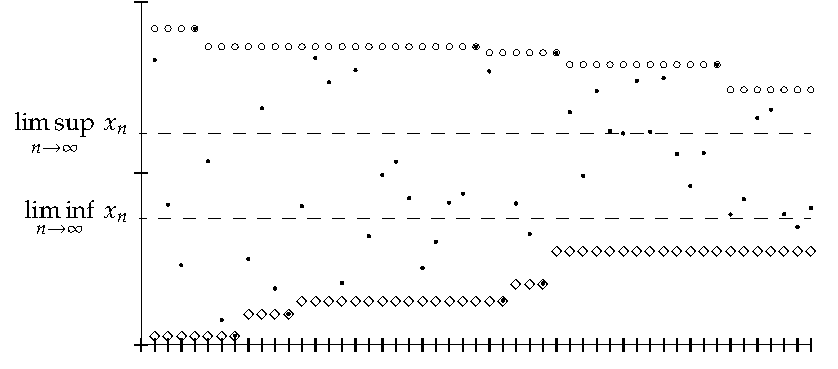
\includegraphics{figures/sequence-limsupliminf_an_bn}
\caption{First 50 terms of an example sequence.  Terms $x_n$ of the sequence are
marked with dots
%mbxSTARTIGNORE
(\raisebox{0.25ex}{\tiny$\bullet$}),
%mbxENDIGNORE
%mbxlatex ($\boldsymbol{\cdot}$),
$a_n$ are marked with
circles ($\circ$), and
$b_n$ are marked with diamonds ($\diamond$).\label{sequence-limsupliminf_an_bn}}
\end{myfigureht}

\begin{example} \label{example:liminfsupex}
Let $\{ x_n \}$ be defined by
\begin{equation*}
x_n :=
\begin{cases}
\frac{n+1}{n} & \text{if } n \text{ is odd,} \\
0             & \text{if } n \text{ is even.}
\end{cases}
\end{equation*}
Let us compute the $\liminf$ and $\limsup$ of this sequence.  See also
\figureref{sequence-limsupliminf_an_bn-example}.  First the
limit inferior:
\begin{equation*}
\liminf_{n\to\infty} \, x_n = 
\lim_{n\to\infty}
\bigl(
\inf \{ x_k : k \geq n \}
\bigr)
=
\lim_{n\to\infty} 0 = 0 .
\end{equation*}
For the limit superior we write
\begin{equation*}
\limsup_{n\to\infty} \, x_n = 
\lim_{n\to\infty}
\bigl(
\sup \{ x_k : k \geq n \}
\bigr) .
\end{equation*}
It is not hard to see that
\begin{equation*}
\sup \{ x_k : k \geq n \} =
\begin{cases}
\frac{n+1}{n}   & \text{if } n \text{ is odd,} \\
\frac{n+2}{n+1} & \text{if } n \text{ is even.}
\end{cases}
\end{equation*}
We leave it to the reader to show that the limit is 1.  That is,
\begin{equation*}
\limsup_{n\to\infty} \, x_n = 1 .
\end{equation*}
Do note that the sequence $\{ x_n \}$ is not a convergent sequence.
\begin{myfigureht}
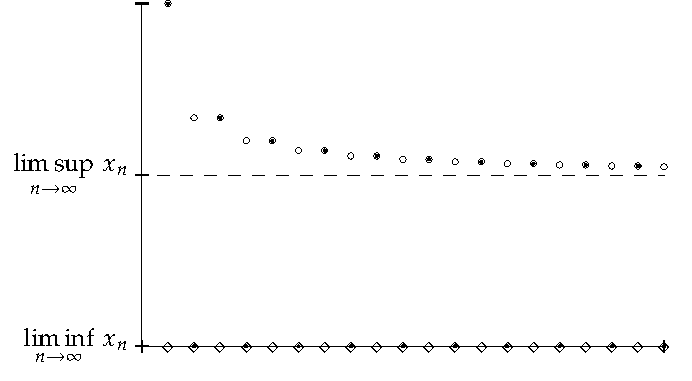
\includegraphics{figures/sequence-limsupliminf_an_bn-example}
\caption{First 20 terms of the sequence in \exampleref{example:liminfsupex}.
The marking is the same as in \figureref{sequence-limsupliminf_an_bn}.
\label{sequence-limsupliminf_an_bn-example}}
\end{myfigureht}
\end{example}

We associate certain subsequences with $\limsup$ and $\liminf$.
It is important to notice that $\{ a_n \}$ and $\{ b_n \}$ are not
necessarily subsequences of $\{ x_n \}$, nor do they have to even 
consist of the same numbers.
For example, for the sequence $\{ \nicefrac{1}{n} \}$,
$b_n = 0$ for all $n \in N$.

\begin{thm} \label{subseqlimsupinf:thm}
If $\{ x_n \}$ is a bounded sequence, then there exists a subsequence
$\{ x_{n_k} \}$ such that
\begin{equation*}
\lim_{k\to \infty} x_{n_k} = \limsup_{n \to \infty} \, x_n .
\end{equation*}
Similarly, there exists a (perhaps different) subsequence
$\{ x_{m_k} \}$ such that
\begin{equation*}
\lim_{k\to \infty} x_{m_k} = \liminf_{n \to \infty} \, x_n .
\end{equation*}
\end{thm}

\begin{proof}
Define $a_n := \sup \{ x_k : k \geq n \}$.
Write
$x := \limsup \, x_n = \lim\, a_n$.  We define the subsequence inductively.
Pick $n_1 := 1$ and suppose we have
defined the subsequence until $n_k$ for some $k$.  Now pick some $m > n_k$
such that
\begin{equation*}
a_{(n_k+1)} - x_m < \frac{1}{k+1} .
\end{equation*}
We can do this as $a_{(n_k+1)}$ is a supremum of the
set $\{ x_n : n \geq n_k + 1 \}$ and hence there are elements
of the sequence arbitrarily close (or even possibly equal) to the supremum.
Set $n_{k+1} :=  m$.  The subsequence $\{ x_{n_k} \}$ is defined.  Next we
need to prove that it converges and has the right limit.

Note that
$a_{(n_{k-1}+1)} \geq a_{n_k}$ (why?) and that $a_{n_{k}} \geq x_{n_k}$.
Therefore, for every $k \geq 2$ we have
\begin{equation*}
\begin{split}
\abs{a_{n_k} - x_{n_k}} & = 
a_{n_k} - x_{n_k}
\\
& \leq
a_{(n_{k-1}+1)} - x_{n_k}
\\
& < \frac{1}{k} .
\end{split}
\end{equation*}

Let us show that $\{ x_{n_k} \}$ converges to $x$.
Note that the subsequence need not be monotone.  Let $\epsilon > 0$ be given.
As $\{ a_n \}$ converges to $x$, then the subsequence
$\{ a_{n_k} \}$ converges to $x$.
Thus there exists an $M_1 \in \N$
such that for all $k \geq M_1$ we have
\begin{equation*}
\abs{a_{n_k} - x} < \frac{\epsilon}{2} .
\end{equation*}
Find an $M_2 \in \N$ such that
\begin{equation*}
\frac{1}{M_2} \leq \frac{\epsilon}{2}.
\end{equation*}
Take $M := \max \{M_1 , M_2 , 2 \}$ and compute.  For all $k \geq M$
we have
\begin{equation*}
\begin{split}
\abs{x- x_{n_k}} & =
\abs{a_{n_k} - x_{n_k} + x - a_{n_k}}
\\
& \leq \abs{a_{n_k} - x_{n_k}} + \abs{x - a_{n_k}}
\\
& < \frac{1}{k} + \frac{\epsilon}{2}
\\
& \leq \frac{1}{M_2} + \frac{\epsilon}{2} \leq \frac{\epsilon}{2} +
\frac{\epsilon}{2} = \epsilon .
\end{split}
\end{equation*}

We leave the statement for $\liminf$ as an exercise.
\end{proof}

\subsection{Using limit inferior and limit superior}

The advantage of $\liminf$ and $\limsup$ is that we can always write them
down for any (bounded) sequence.
If we could somehow compute them, we could also compute the limit of the
sequence if it exists, or show that the sequence diverges.
Working with $\liminf$ and $\limsup$ is a
little bit like working with limits, although there are subtle differences.

\begin{prop} \label{liminfsupconv:prop}
Let $\{ x_n \}$ be a bounded sequence.  Then $\{ x_n \}$ converges
if and only if
\begin{equation*}
\liminf_{n\to \infty} \, x_n = 
\limsup_{n\to \infty} \, x_n.
\end{equation*}
Furthermore, if $\{ x_n \}$ converges, then
\begin{equation*}
\lim_{n\to \infty} x_n = 
\liminf_{n\to \infty} \, x_n = 
\limsup_{n\to \infty} \, x_n.
\end{equation*}
\end{prop}

\begin{proof}
Let $a_n$ and $b_n$ be as in \defnref{liminflimsup:def}.
In particular, for all $n \in \N$,
\begin{equation*}
b_n \leq x_n \leq a_n .
\end{equation*}
If 
$\liminf \, x_n = \limsup \, x_n$, then we know that $\{ a_n \}$ and $\{ b_n \}$
have limits and that these two limits are the same.  By the squeeze lemma
(\lemmaref{squeeze:lemma}), $\{ x_n \}$ converges and
\begin{equation*}
\lim_{n\to \infty} b_n
=
\lim_{n\to \infty} x_n
=
\lim_{n\to \infty} a_n .
\end{equation*}

Now suppose $\{ x_n \}$ converges to $x$.
We know by
\thmref{subseqlimsupinf:thm}
that there exists a subsequence $\{ x_{n_k} \}$
that converges to $\limsup \, x_n$.
As $\{ x_n \}$ converges to $x$,
every subsequence converges to $x$ and
therefore $\limsup \, x_n = \lim\, x_{n_k} = x$.  Similarly, $\liminf \, x_n = x$.
\end{proof}

Limit superior and limit inferior behave nicely
with subsequences.

\begin{prop} \label{prop:subseqslimsupinf}
Suppose $\{ x_n \}$ is a bounded sequence and
$\{ x_{n_k} \}$ is a subsequence.  Then
\begin{equation*}
\liminf_{n\to\infty} \, x_n \leq
\liminf_{k\to\infty} \, x_{n_k} \leq
\limsup_{k\to\infty} \, x_{n_k} \leq
\limsup_{n\to\infty} \, x_n .
\end{equation*}
\end{prop}

\begin{proof}
The middle inequality has been proved already.  We will prove the third
inequality, and leave the first inequality as an exercise.

We want to prove that
$\limsup \, x_{n_k} \leq \limsup \, x_n$.  Define
$a_j := \sup \{ x_k : k \geq j \}$ 
as usual.
Also define
$c_j := \sup \{ x_{n_k} : k \geq j \}$.
It is not true that $c_j$ is necessarily a subsequence of $a_j$.  However,
as $n_k \geq k$ for all $k$, we have that
$\{ x_{n_k} : k \geq j \} \subset \{ x_k : k \geq j \}$.
A supremum of a subset is less than or equal to the supremum of the
set and therefore
\begin{equation*}
c_j \leq a_j .
\end{equation*}
We apply \lemmaref{limandineq:lemma} to conclude 
\begin{equation*}
\lim_{j\to\infty} c_j \leq \lim_{j\to\infty} a_j ,
\end{equation*}
which is the desired conclusion.
\end{proof}

Limit superior and limit inferior
are the largest and smallest
subsequential limits.  If the subsequence $\{ x_{n_k} \}$ in the previous
proposition is convergent, then
$\liminf \, x_{n_k} = \lim\, x_{n_k} = \limsup \, x_{n_k}$.  Therefore,
\begin{equation*}
\liminf_{n\to\infty} \, x_n \leq
\lim_{k\to\infty} x_{n_k} \leq
\limsup_{n\to\infty} \, x_n .
\end{equation*}

Similarly, we get the following useful test for convergence
of a bounded sequence.  We leave the proof as an exercise.

\begin{prop} \label{seqconvsubseqconv:prop}
A bounded sequence $\{ x_n \}$ is convergent and converges to $x$
if and only if
every convergent subsequence
$\{ x_{n_k} \}$ converges to $x$.
\end{prop}

\subsection{Bolzano--Weierstrass theorem}

While it is not true that a bounded sequence is convergent, the
Bolzano--Weierstrass theorem tells us that we can at least find a convergent
subsequence.
The version of Bolzano--Weierstrass 
that we present in this section is the Bolzano--Weierstrass for
sequences.

\begin{thm}[Bolzano--Weierstrass]\index{Bolzano--Weierstrass theorem}\label{thm:bwseq}
Suppose a sequence $\{ x_n \}$ of real numbers is bounded.
Then there exists a convergent subsequence $\{ x_{n_i} \}$.
\end{thm}

\begin{proof}
We use \thmref{subseqlimsupinf:thm}.  It says that there exists
a subsequence whose limit is $\limsup \, x_n$.
\end{proof}

The reader might complain right now that 
\thmref{subseqlimsupinf:thm} is strictly stronger than the
Bolzano--Weierstrass theorem as presented above.  That is true.
However, 
\thmref{subseqlimsupinf:thm} only applies to the real line, but
Bolzano--Weierstrass applies in more general contexts (that is, in $\R^n$)
with pretty much the exact same statement.

As the theorem is so important to analysis, we present an explicit
proof.
The following proof generalizes more easily to different contexts.

\begin{proof}[Alternate proof of Bolzano--Weierstrass]
As the sequence is bounded, then there exist two numbers $a_1 < b_1$
such that $a_1 \leq x_n \leq b_1$ for all $n \in \N$.

We will define a subsequence $\{ x_{n_i} \}$ and two
sequences $\{ a_i \}$ and $\{ b_i \}$, such that
$\{ a_i \}$ is monotone increasing, $\{ b_i \}$ is monotone decreasing,
$a_i \leq x_{n_i} \leq b_i$ and such that $\lim\, a_i = \lim\, b_i$.   That
$x_{n_i}$ converges follows by the \hyperref[squeeze:lemma]{squeeze lemma}.

We define the sequences inductively.  We will always have that $a_i < b_i$,
and that $x_n \in [a_i,b_i]$ for infinitely many
$n \in \N$.
We have already defined $a_1$ and $b_1$.  We take $n_1 := 1$, that is
$x_{n_1} = x_1$.

Suppose that up to some $k \in \N$
we have defined the subsequence $x_{n_1}, x_{n_2}, \ldots,
x_{n_k}$, and the sequences $a_1,a_2,\ldots,a_k$
and $b_1,b_2,\ldots,b_k$.
Let $y := \frac{a_k+b_k}{2}$.
Clearly
$a_k < y < b_k$.  If there exist infinitely many $j \in \N$
such that $x_j \in [a_k,y]$, then set $a_{k+1} := a_k$, $b_{k+1} := y$,
and pick $n_{k+1} > n_{k}$
such that $x_{n_{k+1}} \in [a_k,y]$.  If there are not infinitely many 
$j$ such that 
$x_j \in [a_k,y]$, then it must be true that there are infinitely many $j \in
\N$ such that 
$x_j \in [y,b_k]$.  In this case pick $a_{k+1} := y$, $b_{k+1} := b_k$,
and pick $n_{k+1} > n_{k}$
such that $x_{n_{k+1}} \in [y,b_k]$.

We now have the sequences defined.  What is left to prove is that
$\lim\, a_i = \lim\, b_i$.  The limits exist as the sequences
are monotone.  In the construction,
$b_i - a_i$ is cut in half in each step.  Therefore,
$b_{i+1} - a_{i+1} = \frac{b_i-a_i}{2}$.  By
\hyperref[induction:thm]{induction},
\begin{equation*}
b_i - a_i = \frac{b_1-a_1}{2^{i-1}} .
\end{equation*}

Let $x := \lim\, a_i$.  As $\{ a_i \}$ is monotone,
\begin{equation*}
x = \sup \{ a_i : i \in \N \} .
\end{equation*}
Let $y := \lim\, b_i = \inf \{ b_i : i \in \N \}$.  Since $a_i < b_i$ for
all $i$, then $y \leq x$.
As the sequences are monotone, then
for any $i$ we have (why?)
\begin{equation*}
y-x \leq b_i-a_i = \frac{b_1-a_1}{2^{i-1}} .
\end{equation*}
Because $\frac{b_1-a_1}{2^{i-1}}$ is arbitrarily small and $y-x \geq 0$,
we have $y-x = 0$.  Finish by the \hyperref[squeeze:lemma]{squeeze lemma}.
\end{proof}

Yet another proof of the Bolzano--Weierstrass theorem is to show the
following claim,
which is left as a challenging exercise.
\emph{Claim: Every sequence has a monotone subsequence}.

\subsection{Infinite limits}

Just as for infima and suprema, it is possible to allow certain
limits to be infinite.  That is, we write $\lim \, x_n = \infty$ or
$\lim \, x_n = -\infty$ for certain divergent sequences.

\begin{defn}
\index{infinite limit!of a sequence}\index{limit!infinite}
We say
$\{ x_n \}$ \emph{\myindex{diverges to infinity}}%
\footnote{Sometimes it is said that $\{ x_n \}$ \emph{converges to infinity}.}
if for every $K \in
\R$, there exists an $M \in \N$ such that for all $n \geq M$ we have $x_n >
K$.  In this case we write
\begin{equation*}
\lim_{n \to \infty} x_n := \infty .  
\end{equation*}
Similarly,
if for every $K \in \R$ there exists an $M \in \N$ such that
for all $n \geq M$ we have $x_n < K$, we say $\{ x_n \}$
\emph{\myindex{diverges to minus infinity}} and we write
\begin{equation*}
\lim_{n \to \infty} x_n := -\infty .  
\end{equation*}
\end{defn}

With this definition and allowing $\infty$ and $-\infty$,
we can write $\lim \, x_n$ for any monotone sequence.

\begin{prop} \label{prop:unboundedmonotone}
Suppose $\{ x_n \}$ is a monotone unbounded sequence.  Then
\begin{equation*}
\lim_{n \to \infty} x_n =
\begin{cases}
\infty  & \text{if } \{ x_n \} \text{ is increasing,} \\
-\infty & \text{if } \{ x_n \} \text{ is decreasing.}
\end{cases}
\end{equation*}
\end{prop}

\begin{proof}
The case of monotone increasing follows from
\exerciseref{exercise:infseqlimlims} part c) below.  Let us do
monotone decreasing.  Suppose $\{x_n\}$ is decreasing and unbounded,
that is,
for every $K \in \R$, there is an $M \in \N$ such that $x_M < K$.
By monotonicity $x_n \leq x_M < K$ for all $n \geq M$.   Therefore,
$\lim \, x_n = -\infty$.
\end{proof}

\begin{example}
\begin{equation*}
\lim_{n\to \infty} n = \infty,
\qquad 
\lim_{n\to \infty} n^2 = \infty,
\qquad 
\lim_{n\to \infty} -n = -\infty.
\end{equation*}
We leave verification to the reader.
\end{example}

We may also allow $\liminf$ and $\limsup$ to take on
the values $\infty$ and $-\infty$, so that
we can apply $\liminf$ and $\limsup$
to absolutely any sequence, not just
a bounded one.   Unfortunately, the sequences $\{ a_n \}$ and $\{ b_n \}$
are not sequences of real numbers but of extended real numbers.  In
particular, $a_n$ can equal $\infty$ for some $n$, and $b_n$ can equal
$-\infty$.  So we have no definition for the limits.
But since the extended real numbers are still an ordered set, we
can take suprema and infima.

\begin{defn}
Let $\{ x_n \}$ be an unbounded sequence of real numbers.  Define 
sequences of extended real numbers by
$a_n := \sup \{ x_k : k \geq n \}$ and
$b_n := \inf \{ x_k : k \geq n \}$.
Define\glsadd{not:limsupseq}\glsadd{not:liminfseq}
\index{limit inferior}\index{limit superior}\index{limsup}\index{liminf}
\begin{equation*}
\limsup_{n \to \infty} \, x_n := \inf \{ a_n : n \in \N \}, \qquad \text{and} \qquad
\liminf_{n \to \infty} \, x_n := \sup \{ b_n : n \in \N \}.
\end{equation*}
\end{defn}

This definition agrees with the definition for bounded
sequences whenever $\lim a_n$ or $\lim b_n$ makes sense including
possibly $\infty$ and $-\infty$.

\begin{prop}
Let $\{ x_n \}$ be an unbounded sequence.  Define 
$\{ a_n \}$ and $\{ b_n \}$ as above.
Then $\{ a_n \}$ is decreasing, and $\{ b_n \}$ is increasing.
If $a_n$ is a real number for every $n$, then
$\limsup \, x_n = \lim \, a_n$. 
If $b_n$ is a real number for every $n$, then
$\liminf \, x_n = \lim \, b_n$.
\end{prop}

\begin{proof}
As before,
$a_n = \sup \{ x_k : k \geq n \} \geq \sup \{ x_k : k \geq n+1 \} =
a_{n+1}$.  So $\{ a_n \}$ is decreasing. Similarly, $\{ b_n \}$ is increasing.

If the sequence $\{ a_n \}$ is a sequence of real numbers, then
$\lim a_n = \inf \{ a_n : n \in \N \}$.  This follows from
\propref{prop:monotoneconv} if $\{ a_n \}$ is bounded and \propref{prop:unboundedmonotone} if $\{a_n \}$
is unbounded.  We proceed similarly with $\{ b_n \}$.
\end{proof}

The definition behaves as expected with
$\limsup$ and $\liminf$, see exercises \ref{exercise:infseqlimex}
and \ref{exercise:infseqlimlims}.

\begin{example}
Suppose 
$x_n := 0$ for odd $n$ and $x_n := n$ for even $n$.
Then $a_n = \infty$ for every $n$, since for any $M$,
there exists an even $k$ such that $x_k = k \geq M$.
On the other hand, $b_n = 0$ for all $n$, as
for any $n$,
$\{ b_k : k \geq n \}$ consists of $0$ and nonnegative numbers.
So,
\begin{equation*}
\lim_{n\to \infty} x_n \quad \text{does not exist},
\qquad 
\limsup_{n\to \infty} \, x_n = \infty ,
\qquad 
\liminf_{n\to \infty} \, x_n = 0.
\end{equation*}
\end{example}

\subsection{Exercises}

\begin{exercise}
Suppose $\{ x_n \}$ is a bounded sequence.  Define $a_n$ and
$b_n$ as in \defnref{liminflimsup:def}.  Show that $\{ a_n \}$
and $\{ b_n \}$ are bounded.
\end{exercise}

\begin{exercise}
Suppose $\{ x_n \}$ is a bounded sequence.
Define $b_n$ as in \defnref{liminflimsup:def}.  Show that
$\{ b_n \}$ is an increasing sequence.
\end{exercise}

\begin{exercise}
Finish the proof of \propref{prop:subseqslimsupinf}.  That is,
suppose $\{ x_n \}$ is a bounded sequence and
$\{ x_{n_k} \}$ is a subsequence.  Prove
$\displaystyle \liminf_{n\to\infty}\, x_n \leq
\liminf_{k\to\infty}\, x_{n_k}$.
\end{exercise}

\begin{exercise}
Prove \propref{seqconvsubseqconv:prop}.
\end{exercise}

\begin{exercise}
\leavevmode
\begin{enumerate}[a)]
\item
Let $x_n := \dfrac{{(-1)}^n}{n}$.
Find $\limsup \, x_n$ and $\liminf \, x_n$.
\item
Let $x_n := \dfrac{(n-1){(-1)}^n}{n}$.
Find $\limsup \, x_n$ and $\liminf \, x_n$.
\end{enumerate}
\end{exercise}

\begin{exercise}
Let $\{ x_n \}$ and $\{ y_n \}$ be bounded sequences such that
$x_n \leq y_n$ for all $n$.  Then show that
\begin{equation*}
\limsup_{n\to\infty} \, x_n \leq
\limsup_{n\to\infty} \, y_n
\end{equation*}
and
\begin{equation*}
\liminf_{n\to\infty} \, x_n \leq
\liminf_{n\to\infty} \, y_n .
\end{equation*}
\end{exercise}

\begin{exercise}
Let $\{ x_n \}$ and $\{ y_n \}$ be bounded sequences.
\begin{enumerate}[a)]
\item
Show that $\{ x_n + y_n \}$ is bounded.
\item
Show that
\begin{equation*}
(\liminf_{n\to \infty}\, x_n)
+
(\liminf_{n\to \infty}\, y_n)
\leq
\liminf_{n\to \infty}\, (x_n+y_n) .
\end{equation*}
Hint: Find a subsequence $\{ x_{n_i}+y_{n_i} \}$ of $\{ x_n + y_n \}$
that converges.
Then find a subsequence $\{ x_{n_{m_i}} \}$ of $\{ x_{n_i} \}$ that converges.
Then apply what you know about limits.
\item
Find an explicit $\{ x_n \}$ and $\{ y_n \}$ such that
\begin{equation*}
(\liminf_{n\to \infty}\, x_n)
+
(\liminf_{n\to \infty}\, y_n)
<
\liminf_{n\to \infty}\, (x_n+y_n) .
\end{equation*}
Hint: Look for examples that do not have a limit.
\end{enumerate}
\end{exercise}

\begin{samepage}
\begin{exercise}
Let $\{ x_n \}$ and $\{ y_n \}$ be bounded sequences (from the previous
exercise we know that $\{ x_n + y_n \}$ is bounded).
\begin{enumerate}[a)]
\item
Show that
\begin{equation*}
(\limsup_{n\to \infty}\, x_n)
+
(\limsup_{n\to \infty}\, y_n)
\geq
\limsup_{n\to \infty}\, (x_n+y_n) .
\end{equation*}
Hint: See previous exercise.
\item
Find an explicit $\{ x_n \}$ and $\{ y_n \}$ such that
\begin{equation*}
(\limsup_{n\to \infty}\, x_n)
+
(\limsup_{n\to \infty}\, y_n)
>
\limsup_{n\to \infty}\, (x_n+y_n) .
\end{equation*}
Hint: See previous exercise.
\end{enumerate}
\end{exercise}
\end{samepage}

\begin{exercise}
If $S \subset \R$ is a set, then $x \in \R$ is a \emph{\myindex{cluster
point}}
if for every $\epsilon > 0$, the set $(x-\epsilon,x+\epsilon) \cap S
\setminus \{ x \}$ is not empty.  That is, if there are points of $S$
arbitrarily close to $x$.
For example, $S := \{ \nicefrac{1}{n} : n \in \N \}$ has a unique (only
one) cluster point $0$, but $0 \notin S$.
Prove the following version of the Bolzano--Weierstrass theorem:

\medskip

\noindent
\emph{\textbf{Theorem.} Let $S \subset \R$ be a bounded infinite set,
then there exists at least one cluster point of $S$}.

\medskip

Hint: If $S$ is infinite, then $S$ contains a countably infinite subset.
That is, there is a sequence $\{ x_n \}$ of distinct numbers in $S$.
\end{exercise}

\begin{samepage}
\begin{exercise}[Challenging]
\leavevmode
\begin{enumerate}[a)]
\item
Prove that any sequence contains a monotone subsequence.
Hint: Call $n \in \N$ a \emph{peak} if $a_m \leq a_n$ for all $m \geq n$.  
There are two possibilities: Either the sequence has at most finitely many
peaks,
or it has infinitely many peaks.
\item
Conclude the Bolzano--Weierstrass theorem.
\end{enumerate}
\end{exercise}
\end{samepage}

\begin{exercise}
Prove a stronger version of \propref{seqconvsubseqconv:prop}.
Suppose $\{ x_n \}$ is a sequence such that every subsequence $\{
x_{n_i} \}$ has a subsequence
$\{ x_{n_{m_i}} \}$ that converges to $x$.
\begin{enumerate}[a)]
\item
First show that $\{ x_n \}$ is
bounded.
\item
Now show that $\{ x_n \}$ converges to $x$.
\end{enumerate}
\end{exercise}

\begin{exercise}
Let $\{x_n\}$ be a bounded sequence.
\begin{enumerate}[a)]
\item
Prove that there exists an $s$ such that for any $r > s$ there exists 
an $M \in \N$ such that for all $n \geq M$ we have
$x_n < r$.
\item
If $s$ is a number as in a), then prove $\limsup \, x_n \leq s$.
\item
Show that if $S$ is the set of all $s$ as in a), then
$\limsup \, x_n = \inf \, S$.
\end{enumerate}
\end{exercise}

\begin{exercise}[Easy] \label{exercise:infseqlimex}
Suppose $\{ x_n \}$ is such that $\liminf \, x_n = -\infty$, $\limsup \, x_n
= \infty$.
\begin{enumerate}[a)]
\item
Show that $\{ x_n \}$ is not convergent, and also
that neither $\lim \, x_n = \infty$ nor $\lim \, x_n =
-\infty$
is true.
\item
Find an example of such a sequence.
\end{enumerate}
\end{exercise}

\begin{exercise} \label{exercise:infseqlimlims}
Let $\{ x_n \}$ be a sequence.
\begin{enumerate}[a)]
\item
Show that
$\lim \, x_n = \infty$ if and only if $\liminf \, x_n = \infty$.
\item
Then show that $\lim \, x_n = - \infty$ if and only if $\limsup \, x_n =
-\infty$.
\item
If $\{ x_n \}$ is monotone increasing, show that either
$\lim \, x_n$ exists and is finite or $\lim \, x_n = \infty$.  In either
case, $\lim \, x_n = \sup \{ x_n : n \in \N \}$.
\end{enumerate}
\end{exercise}

\begin{exercise} \label{exercise:strongerratiotest2}
Prove the following stronger version of \lemmaref{seq:ratiotest}, the ratio
test.
Suppose $\{ x_n \}$ is a sequence such that $x_n \not= 0$ for all
$n$.
\begin{enumerate}[a)]
\item
Prove that if
\begin{equation*}
\limsup_{n \to \infty} \frac{\abs{x_{n+1}}}{\abs{x_n}} < 1 ,
\end{equation*}
then $\{ x_n \}$ converges to $0$.
\item
Prove that if
\begin{equation*}
\liminf_{n \to \infty} \frac{\abs{x_{n+1}}}{\abs{x_n}} > 1 ,
\end{equation*}
then $\{ x_n \}$ is unbounded.
\end{enumerate}
\end{exercise}

\begin{exercise}
Suppose $\{ x_n \}$ is a bounded sequence, $a_n := \sup \{ x_k : k \geq n \}$
as before.  Suppose that for some $\ell \in \N$,
$a_\ell \notin \{ x_k : k \geq \ell \}$.  Then show that $a_j = a_\ell$ for all $j \geq \ell$, and hence
$\limsup\, x_n = a_\ell$.
\end{exercise}

\begin{exercise}
Suppose $\{ x_n \}$ is a sequence,
and $a_n := \sup \{ x_k : k \geq n \}$ and
$b_n := \sup \{ x_k : k \geq n \}$ as before.
\begin{enumerate}[a)]
\item
Prove that if $a_\ell = \infty$ for some $\ell \in \N$, then 
$\limsup\, x_n = \infty$.
\item
Prove that if $b_\ell = -\infty$ for some $\ell \in \N$, then 
$\liminf\, x_n = -\infty$.
\end{enumerate}
\end{exercise}

\begin{exercise}
Suppose $\{ x_n \}$ is a sequence
such that both $\liminf\, x_n$ and
$\limsup\, x_n$  are finite.  Prove that $\{ x_n \}$ is bounded.
\end{exercise}

\begin{exercise}
Suppose $\{ x_n \}$ is a bounded sequence, and $\epsilon > 0$ is given.
Prove that there exists an $M$ such that for all $k \geq M$ we have
\begin{equation*}
x_k - \Bigl(\limsup_{n\to\infty}\, x_n\Bigr) < \epsilon \qquad \text{and} \qquad
\Bigl(\liminf_{n\to\infty}\, x_n\Bigr) - x_k < \epsilon .
\end{equation*}
\end{exercise}


%%%%%%%%%%%%%%%%%%%%%%%%%%%%%%%%%%%%%%%%%%%%%%%%%%%%%%%%%%%%%%%%%%%%%%%%%%%%%%

\sectionnewpage
\section{Cauchy sequences}
\label{sec:cauchy}

\sectionnotes{0.5--1 lecture}

Often we wish to describe a certain number 
by a sequence that converges to it.  In this case, it is impossible to use the
number itself in the proof that the sequence converges.
It would be nice if we could check for convergence without knowing
the limit.

\begin{defn}
A sequence $\{ x_n \}$ is a \emph{\myindex{Cauchy sequence}}%
\footnote{%
Named after the French mathematician
\href{https://en.wikipedia.org/wiki/Cauchy}{Augustin-Louis Cauchy} (1789--1857).} if
for every $\epsilon > 0$ there exists an $M \in \N$ such that
for all $n \geq M$ and all $k \geq M$ we have
\begin{equation*}
\abs{x_n - x_k} < \epsilon .
\end{equation*}
\end{defn}

Intuitively it means that the terms of the sequence are eventually
arbitrarily close to each other.  We would expect such a sequence to be
convergent.  It turns out that is true because $\R$ has the
\hyperref[defn:lub]{least-upper-bound property}.  First, let us look at some examples.

\begin{example}
The sequence $\{ \nicefrac{1}{n} \}$ is a Cauchy sequence.

Proof:  Given $\epsilon > 0$, find $M$ such that
$M > \nicefrac{2}{\epsilon}$.  Then for $n,k \geq M$
we have that $\nicefrac{1}{n} < \nicefrac{\epsilon}{2}$
and
$\nicefrac{1}{k} < \nicefrac{\epsilon}{2}$.  Therefore, for $n, k \geq M$
we have
\begin{equation*}
\abs{\frac{1}{n} - \frac{1}{k}}
\leq
\abs{\frac{1}{n}} + \abs{\frac{1}{k}}
< \frac{\epsilon}{2} + \frac{\epsilon}{2} = \epsilon.
\end{equation*}
\end{example}

\begin{example}
The sequence $\{ \frac{n+1}{n} \}$ is a Cauchy sequence.

Proof:  Given $\epsilon > 0$, find $M$ such that
$M > \nicefrac{2}{\epsilon}$.  Then for $n,k \geq M$
we have that $\nicefrac{1}{n} < \nicefrac{\epsilon}{2}$
and
$\nicefrac{1}{k} < \nicefrac{\epsilon}{2}$.  Therefore, for $n, k \geq M$
we have
\begin{equation*}
\begin{split}
\abs{\frac{n+1}{n} - \frac{k+1}{k}}
& =
\abs{\frac{k(n+1)-n(k+1)}{nk}}
\\
& =
\abs{\frac{kn+k-nk-n}{nk}}
\\
& =
\abs{\frac{k-n}{nk}}
\\
& \leq
\abs{\frac{k}{nk}}
+
\abs{\frac{-n}{nk}}
\\
& = \frac{1}{n} + \frac{1}{k}
< \frac{\epsilon}{2} + \frac{\epsilon}{2} = \epsilon .
\end{split}
\end{equation*}
\end{example}

\begin{prop}
A Cauchy sequence is bounded.
\end{prop}

\begin{proof}
Suppose $\{ x_n \}$ is Cauchy.  Pick $M$ such that for all
$n,k \geq M$ we have $\abs{x_n-x_k} < 1$.  In particular, 
for all $n \geq M$,
\begin{equation*}
\abs{x_n - x_M} < 1 .
\end{equation*}
By the reverse triangle inequality,
$\abs{x_n} - \abs{x_M} \leq \abs{x_n - x_M} < 1$.  Hence for $n \geq M$,
\begin{equation*}
\abs{x_n} < 1 + \abs{x_M}.
\end{equation*}
Let
\begin{equation*}
B := \max \{ \abs{x_1}, \abs{x_2}, \ldots, \abs{x_{M-1}}, 1+ \abs{x_M} \} .
\end{equation*}
Then $\abs{x_n} \leq B$ for all $n \in \N$.
\end{proof}

\begin{thm}
A sequence of real numbers is Cauchy if and only if it converges.
\end{thm}

\begin{proof}
Let $\epsilon > 0$ be given and
suppose $\{ x_n \}$ converges to $x$.  Then there 
exists an $M$ such that for $n \geq M$,
\begin{equation*}
\abs{x_n - x} < \frac{\epsilon}{2} .
\end{equation*}
Hence for $n \geq M$ and $k \geq M$,
\begin{equation*}
\abs{x_n - x_k} = 
\abs{x_n - x + x - x_k}
\leq \abs{x_n-x} + \abs{x-x_k} < \frac{\epsilon}{2} + \frac{\epsilon}{2} =
\epsilon .
\end{equation*}

Alright, that direction was easy.  Now suppose $\{ x_n \}$ is Cauchy.
We have shown that $\{ x_n \}$ is bounded.
For a bounded sequence, liminf and limsup exist, and this is
where we use the
\hyperref[defn:lub]{least-upper-bound property}.
If we show that
\begin{equation*}
\liminf_{n\to \infty} \, x_n = \limsup_{n\to\infty} \, x_n ,
\end{equation*}
then $\{ x_n \}$ must be convergent by \propref{liminfsupconv:prop}.


Define $a := \limsup \, x_n$ and
$b := \liminf \, x_n$.
By \thmref{subseqlimsupinf:thm}, there exist subsequences
$\{ x_{n_i} \}$ and
$\{ x_{m_i} \}$, such that
\begin{equation*}
\lim_{i\to\infty} x_{n_i} = a
\qquad \text{and} \qquad
\lim_{i\to\infty} x_{m_i} = b.
\end{equation*}
Given an $\epsilon > 0$,
there exists an $M_1$ such that for all $i \geq M_1$
we have $\abs{x_{n_i} - a} < \nicefrac{\epsilon}{3}$ and
an $M_2$ such that for all $i \geq M_2$ we have
$\abs{x_{m_i} - b} < \nicefrac{\epsilon}{3}$.  There also exists an $M_3$
such that for all $n,k \geq M_3$ we have
$\abs{x_n-x_k} < \nicefrac{\epsilon}{3}$.  Let $M := \max \{ M_1, M_2, M_3 \}$.
If $i \geq M$, then $n_i \geq M$ and $m_i \geq M$.  Hence
\begin{equation*}
\begin{split}
\abs{a-b} & =
\abs{a-x_{n_i}+x_{n_i}
-x_{m_i}+x_{m_i}
-b} \\
& \leq
\abs{a-x_{n_i}}
+ \abs{x_{n_i} -x_{m_i}}
+ \abs{x_{m_i} -b} \\
& <
\frac{\epsilon}{3}
+
\frac{\epsilon}{3}
+
\frac{\epsilon}{3}
= \epsilon .
\end{split}
\end{equation*}
As $\abs{a-b} < \epsilon$ for all $\epsilon > 0$, then $a=b$ and 
the sequence converges.
\end{proof}

\begin{remark}
The statement of this proposition is sometimes used to define the
completeness property of the real numbers.  We say a set is
\emph{\myindex{Cauchy-complete}} (or sometimes just \emph{\myindex{complete}})
if every Cauchy sequence converges.
Above we proved that
as $\R$ has the \hyperref[defn:lub]{least-upper-bound property}, then $\R$ is 
Cauchy-complete.
We can \myquote{complete} $\Q$ by \myquote{throwing in} just enough points to make all
Cauchy sequences converge (we omit the details).
The resulting field has the
least-upper-bound property.
The advantage of using Cauchy
sequences to define completeness is that this idea generalizes to
more abstract settings.
\end{remark}

The Cauchy criterion is stronger than 
$\abs{x_{n+1}-x_n}$ (or $\abs{x_{n+j}-x_n}$ for a fixed $j$) going to zero as
$n$ goes to
infinity.  When we get to the partial sums of the harmonic series
(see \exampleref{example:harmonicseries} in the next section), we will have
a sequence such that $x_{n+1}-x_n = \nicefrac{1}{n}$, yet $\{ x_n \}$ is
divergent.  In fact, for that sequence,
$\lim_{n\to\infty} \abs{x_{n+j}-x_n} = 0$ for
any $j \in \N$ (confer \exerciseref{exercise:badnocauchy}).
The key point in the definition of Cauchy is that $n$ and $k$
vary independently and can be arbitrarily far apart.

\subsection{Exercises}

\begin{exercise}
Prove that $\{ \frac{n^2-1}{n^2} \}$ is Cauchy using directly the definition
of Cauchy sequences.
\end{exercise}

\begin{exercise}
Let $\{ x_n \}$ be a sequence such that
there exists a $0 < C < 1$ such that
\begin{equation*}
\abs{x_{n+1} - x_n} \leq C \abs{x_{n}-x_{n-1}} .
\end{equation*}
Prove that $\{ x_n \}$ is Cauchy.
Hint:  You can freely use the formula (for $C \not= 1$)
\begin{equation*}
1+ C+ C^2 + \cdots + C^n = \frac{1-C^{n+1}}{1-C}.
\end{equation*}
\end{exercise}

\begin{exercise}[Challenging]
Suppose $F$ is an ordered field that contains the rational numbers
$\Q$, such that $\Q$ is dense,
that is: Whenever $x,y \in F$ are such that $x < y$,
then there exists a $q \in \Q$ such that $x < q < y$.
Say a sequence $\{ x_n \}_{n=1}^\infty$ of rational numbers is Cauchy
if given any $\epsilon \in \Q$ with $\epsilon > 0$, there exists
an $M$ such that for all $n,k \geq M$ we have $\abs{x_n-x_k} < \epsilon$.
Suppose any Cauchy sequence of rational numbers has a limit in $F$.
Prove that $F$ has the \hyperref[defn:lub]{least-upper-bound property}.
\end{exercise}

\begin{exercise}
Let $\{ x_n \}$ and $\{ y_n \}$ be sequences such
that $\lim\, y_n =0$.  Suppose that for all $k \in \N$
and
for all $m \geq k$ we have
\begin{equation*}
\abs{x_m-x_k} \leq y_k .
\end{equation*}
Show that $\{ x_n \}$ is Cauchy.
\end{exercise}

\begin{exercise}
Suppose a Cauchy sequence $\{ x_n \}$ is such that for every $M \in \N$,
there exists a $k \geq M$ and an $n \geq M$ such that
$x_k < 0$ and $x_n > 0$.  Using simply the definition of a Cauchy sequence
and of a convergent sequence, show that
the sequence converges to $0$.
\end{exercise}

\begin{exercise}
Suppose $\abs{x_n-x_k} \leq \nicefrac{n}{k^2}$ for all $n$ and $k$.
Show that $\{ x_n \}$ is Cauchy.
\end{exercise}

\begin{exercise}
Suppose $\{ x_n \}$ is a Cauchy sequence such that for infinitely many
$n$, $x_n = c$.  Using only the definition of Cauchy sequence prove 
that $\lim\, x_n = c$.
\end{exercise}

\begin{exercise}
True or false, prove or find a counterexample:  If $\{ x_n \}$ is a Cauchy
sequence, then there exists an $M$
such that for all $n \geq M$ we have
$\abs{x_{n+1}-x_n}
\leq
\abs{x_{n}-x_{n-1}}$.
\end{exercise}


%%%%%%%%%%%%%%%%%%%%%%%%%%%%%%%%%%%%%%%%%%%%%%%%%%%%%%%%%%%%%%%%%%%%%%%%%%%%%%

\sectionnewpage
\section{Series}
\label{sec:series}

\sectionnotes{2 lectures}

A fundamental object in mathematics is that of a series.  In fact, when
the foundations of analysis were being developed, the motivation was to
understand series.  Understanding series is important in applications
of analysis.  For example, solving differential equations often includes
series, and differential equations are the basis for understanding
almost all of modern science.

\subsection{Definition}

\begin{defn}
Given a sequence $\{ x_n \}$, we write the formal object
\begin{equation*}
\sum_{n=1}^\infty x_n
\qquad
\text{or sometimes just}
\qquad
\sum x_n
\end{equation*}
\glsadd{not:series}
and call it a \emph{\myindex{series}}.  A series
\emph{converges}\index{convergent!series}, if the sequence $\{ s_k \}$
defined by
\glsadd{not:finitesum}
\begin{equation*}
s_k := \sum_{n=1}^k x_n = x_1 + x_2 + \cdots + x_k ,
\end{equation*}
converges.
The numbers $s_k$ are called
\emph{\myindex{partial sums}}.
If $x := \lim\, s_k$, we write
\begin{equation*}
\sum_{n=1}^\infty x_n =  x .
\end{equation*}
In this case, we cheat a little and treat
$\sum_{n=1}^\infty x_n$ as a number.

If the sequence $\{ s_k \}$ diverges,
we say the series is \emph{divergent}\index{divergent!series}.
In this case, $\sum x_n$ is simply a formal object and not a number.
\end{defn}

In other words, for a convergent series we have
\begin{equation*}
\sum_{n=1}^\infty x_n
=
\lim_{k\to\infty} 
\sum_{n=1}^k x_n .
\end{equation*}
We only have this equality if the limit on
the right actually exists.  If the series does not converge, the right-hand
side does not make sense (the limit does not exist).
Therefore, be careful as 
$\sum x_n$ means two different things (a notation for the series itself 
or the limit of the partial sum), and you must use context
to distinguish.

\begin{remark}
Before going further, let us remark that it is sometimes convenient to start
the series at an index different from 1.  That is, for example we can write
\begin{equation*}
\sum_{n=0}^\infty r^n = \sum_{n=1}^\infty r^{n-1} .
\end{equation*}
The left-hand side is more convenient to write.
\end{remark}

\begin{remark}
It is common to write the series $\sum x_n$ as
\begin{equation*}
x_1 + x_2 + x_3 + \cdots
\end{equation*}
with the understanding that the ellipsis indicates a series and
not a simple sum.  We do not use this notation as it often leads to 
mistakes in proofs.
\end{remark}

\begin{example}
The series
\begin{equation*}
\sum_{n=1}^\infty \frac{1}{2^n}
\end{equation*}
converges and the limit is 1.  That is,
\begin{equation*}
\sum_{n=1}^\infty \frac{1}{2^n} = 
\lim_{k\to\infty} \sum_{n=1}^k \frac{1}{2^n} = 
1 .
\end{equation*}

Proof: First we prove the following equality
\begin{equation*}
\left( \sum_{n=1}^k \frac{1}{2^n} \right)
+ \frac{1}{2^k}
= 1 .
\end{equation*}
The equality is immediate when $k=1$.  The proof for general $k$
follows by \hyperref[induction:thm]{induction}, which we leave to the
reader.  See \figureref{figcutseries} for an illustration.
\begin{myfigureht}
\subimport*{figures/}{figcutseries.pdf_t}
\caption{The equality 
$\left( \sum_{n=1}^k \frac{1}{2^n} \right)
+ \frac{1}{2^k}
= 1$ illustrated for $k=3$.\label{figcutseries}}
\end{myfigureht}

Let $s_k$ be the partial sum.  We write
\begin{equation*}
\abs{
1 - s_k 
}
=
\abs{
1 - 
\sum_{n=1}^k \frac{1}{2^n}
}
=
\abs{\frac{1}{2^k}} = 
\frac{1}{2^k} .
\end{equation*}
The sequence $\{ \frac{1}{2^k} \}$ and therefore $\{ \abs{1-s_k} \}$
converges to zero.  So, $\{ s_k \}$ converges to 1.
\end{example}

\begin{prop} \label{geometric:prop}
Suppose
$-1 < r < 1$.  Then the \emph{\myindex{geometric series}}
$\sum_{n=0}^\infty r^n$ converges, and
\begin{equation*}
\sum_{n=0}^\infty r^n = \frac{1}{1-r} .
\end{equation*}
\end{prop}

Details of the proof are left as an exercise.
The proof consists of showing 
\begin{equation*}
\sum_{n=0}^{k-1} r^n = \frac{1-r^k}{1-r} ,
\end{equation*}
and then taking the limit as $k$ goes to $\infty$.
Geometric series is one of the most important series, and in fact it is
one of the few series for which we can so explicitly find the limit.

\medskip

We have the following analogue of the tail of a sequence.

\begin{prop}
Let $\sum x_n$ be a series.  Let $M \in \N$.  Then
\begin{equation*}
\sum_{n=1}^\infty x_n \quad \text{converges if and only if} \quad
\sum_{n=M}^\infty x_n \quad \text{converges.}
\end{equation*}
\end{prop}

\begin{proof}
We look at partial sums of the two series (for $k \geq M$)
\begin{equation*}
\sum_{n=1}^{k} x_n
=
\left(
\sum_{n=1}^{M-1} x_n
\right)
+
\sum_{n=M}^{k} x_n .
\end{equation*}
Note that 
$\sum_{n=1}^{M-1} x_n$ is a fixed number.  Now use
\propref{prop:contalg} to finish the proof.
\end{proof}

\subsection{Cauchy series}

\begin{defn}
A series $\sum x_n$ is said to be \emph{Cauchy} or a
\emph{Cauchy series}\index{Cauchy series},
if the sequence of partial sums $\{ s_n \}$ is a Cauchy sequence.
\end{defn}

A sequence of real numbers converges if and only if it is
Cauchy.  Therefore, a series is convergent if and only if it is Cauchy.
The series $\sum x_n$ is Cauchy if for every $\epsilon > 0$,
there exists an $M \in \N$, such that for every $n \geq M$
and $k \geq M$ we have
\begin{equation*}
\abs{ \left( \sum_{j=1}^k x_j \right) - \left( \sum_{j=1}^n x_j \right) }
< \epsilon .
\end{equation*}
Without loss of generality we assume $n < k$.  Then we write
\begin{equation*}
\abs{ \left( \sum_{j=1}^k x_j \right) - \left( \sum_{j=1}^n x_j \right) }
=
\abs{ \sum_{j={n+1}}^k x_j }
< \epsilon .
\end{equation*}
We have proved the following simple proposition.

\begin{prop} \label{prop:cachyser}
The series $\sum x_n$ is Cauchy if for every $\epsilon > 0$, 
there exists an $M \in \N$ such that for every $n \geq M$
and every $k > n$ we have
\begin{equation*}
\abs{ \sum_{j={n+1}}^k x_j }
< \epsilon .
\end{equation*}
\end{prop}

\subsection{Basic properties}

\begin{prop}
Let $\sum x_n$ be a convergent series.  Then
the sequence $\{ x_n \}$ is convergent and
\begin{equation*}
\lim_{n\to\infty} x_n = 0.
\end{equation*}
\end{prop}

\begin{proof}
Let $\epsilon > 0$ be given.  As $\sum x_n$ is convergent, it is Cauchy.
Thus we find an $M$ such that for every $n \geq M$ we have
\begin{equation*}
\epsilon > 
\abs{ \sum_{j={n+1}}^{n+1} x_j }
=
\abs{ x_{n+1} } .
\end{equation*}
Hence for every $n \geq M+1$ we have $\abs{x_{n}} < \epsilon$.
\end{proof}

\begin{example}
If $r \geq 1$ or $r \leq -1$, then the geometric series $\sum_{n=0}^\infty r^n$
diverges.

Proof: $\abs{r^n} = \abs{r}^n \geq 1^n = 1$.  So the terms do not go to zero
and the series cannot converge.
\end{example}

So if a series converges, the terms of the series go to zero.
The implication, however, goes only one way.
Let us give an example.

\begin{example} \label{example:harmonicseries}
The series $\sum \frac{1}{n}$ diverges (despite the fact that $\lim
\frac{1}{n} = 0$).  This is the famous \emph{\myindex{harmonic series}}%
\footnote{The divergence of the harmonic series was known 
before the theory of series was made rigorous.  In fact the proof we
give is the earliest proof and was given by
\href{https://en.wikipedia.org/wiki/Oresme}{Nicole Oresme}
(1323?--1382).}.

Proof: We will show that the sequence of partial sums is unbounded, and hence
cannot converge.
Write the partial sums $s_n$ for $n = 2^k$ as:
\begin{align*}
 s_1 & = 1 , \\
 s_2 & = \left( 1 \right) + \left( \frac{1}{2} \right) , \\
 s_4 & = \left( 1 \right) + \left( \frac{1}{2} \right) +
        \left( \frac{1}{3} + \frac{1}{4} \right) , \\
 s_8 & = \left( 1 \right) + \left( \frac{1}{2} \right) +
        \left( \frac{1}{3} + \frac{1}{4} \right) +
        \left( \frac{1}{5} + \frac{1}{6} + \frac{1}{7} + \frac{1}{8} \right) , \\
& ~~ \vdots \\
 s_{2^k} & = 
1 + 
\sum_{j=1}^k
\left(
\sum_{m=2^{j-1}+1}^{2^j} \frac{1}{m}
\right) .
\end{align*}
Notice $\nicefrac{1}{3} + \nicefrac{1}{4} \geq \nicefrac{1}{4} + \nicefrac{1}{4} =
\nicefrac{1}{2}$ and
$\nicefrac{1}{5} + \nicefrac{1}{6} + \nicefrac{1}{7} + \nicefrac{1}{8}
\geq \nicefrac{1}{8} + \nicefrac{1}{8} + \nicefrac{1}{8} + \nicefrac{1}{8} =
\nicefrac{1}{2}$.  More generally
\begin{equation*}
\sum_{m=2^{k-1}+1}^{2^k} \frac{1}{m}
\geq
\sum_{m=2^{k-1}+1}^{2^k} \frac{1}{2^k}
=
(2^{k-1}) \frac{1}{2^k} = \frac{1}{2} .
\end{equation*}
Therefore,
\begin{equation*}
s_{2^k} = 
1 + 
\sum_{j=1}^k
\left(
\sum_{m=2^{j-1}+1}^{2^j} \frac{1}{m}
\right) 
\geq
1 + \sum_{j=1}^k \frac{1}{2} = 1 + \frac{k}{2} .
\end{equation*}
As $\{ \frac{k}{2} \}$ is unbounded by the
\hyperref[thm:arch:i]{Archimedean property}, that means that
$\{ s_{2^k} \}$ is unbounded, and therefore $\{ s_n \}$ is unbounded.
Hence $\{ s_n \}$ diverges, and consequently $\sum \frac{1}{n}$ diverges.
\end{example}

Convergent series are linear.  That is, we can multiply them by constants
and add them and these operations are done term by term.

\begin{prop}[Linearity of series]\index{linearity of series}
Let $\alpha \in \R$ and $\sum x_n$ and $\sum y_n$ be
convergent series.  Then
\begin{enumerate}[(i)]
\item
$\sum \alpha x_n$ is a convergent series and
\begin{equation*}
\sum_{n=1}^\infty \alpha x_n
=
\alpha \sum_{n=1}^\infty x_n .
\end{equation*}
\item
$\sum ( x_n + y_n )$ is a convergent series and
\begin{equation*}
\sum_{n=1}^\infty ( x_n + y_n ) 
=
\left( \sum_{n=1}^\infty x_n \right)
+
\left( \sum_{n=1}^\infty y_n \right) .
\end{equation*}
\end{enumerate}
\end{prop}

\begin{proof}
For the first item,
we simply write the $k$th partial sum
\begin{equation*}
\sum_{n=1}^k \alpha x_n
=
\alpha \left( \sum_{n=1}^k x_n \right) .
\end{equation*}
We look at the right-hand side and note that the constant multiple of
a convergent sequence
is convergent.  Hence, we take the limit of both sides to obtain
the result.

For the second item we also look at the
$k$th partial sum
\begin{equation*}
\sum_{n=1}^k ( x_n + y_n ) 
=
\left( \sum_{n=1}^k x_n \right)
+
\left( \sum_{n=1}^k y_n \right) .
\end{equation*}
We look at the right-hand side and note that the sum of convergent sequences
is convergent.  Hence, we take the limit of both sides to obtain
the proposition.
\end{proof}

An example of a useful application of the first item is the following
formula.  Suppose $\abs{r} < 1$ and $j \in \N$, then
\begin{equation*}
\sum_{n=j}^\infty r^n = \frac{r^j}{1-r} .
\end{equation*}
The formula follows by using the geometric series and multiplying by
$r^j$:
\begin{equation*}
r^j \sum_{n=0}^\infty r^n =
\sum_{n=0}^\infty r^{n+j}
=
\sum_{n=j}^\infty r^n .
\end{equation*}

Multiplying series is not as simple as adding, see the next
section.
It is not true, of course, that we multiply
term by term.  That strategy does not work even for finite sums:
$(a+b)(c+d) \not= ac+bd$.

\subsection{Absolute convergence}

As monotone sequences are easier to work with than arbitrary sequences, it
is usually easier to work with series $\sum x_n$, where $x_n \geq 0$ for
all $n$.  The sequence of partial sums is then monotone increasing
and converges if it is bounded above.
Let us formalize this statement as a proposition.

\begin{prop}
If $x_n \geq 0$ for all $n$, then $\sum x_n$ converges if and only if
the sequence of partial sums is bounded above.
\end{prop}

As the limit of a monotone increasing sequence is the supremum, then
when $x_n \geq 0$ for all $n$, we have the
inequality
\begin{equation*}
\sum_{n=1}^k x_n \leq
\sum_{n=1}^\infty x_n .
\end{equation*}
If we allow infinite limits, the inequality still
holds even when the series diverges to infinity, although in that case it is not
terribly useful.

We will see that the following common criterion for convergence of series 
has big implications for how the series can be manipulated.

\begin{defn}
A series $\sum x_n$
\emph{\myindex{converges absolutely}}\index{absolute convergence} if
the series $\sum \abs{x_n}$ converges.
If a series converges, but does not converge absolutely, we say
it is \emph{\myindex{conditionally convergent}}.
\end{defn}

\begin{prop}
If the series $\sum x_n$ converges absolutely, then it converges.
\end{prop}

\begin{proof}
A series is convergent if and only if it is Cauchy.  Hence
suppose $\sum \abs{x_n}$ is Cauchy.  That is, for every $\epsilon > 0$,
there exists an $M$ such that for all $k \geq M$ and all $n > k$ we have 
\begin{equation*}
\sum_{j=k+1}^n \abs{x_j} 
=
\abs{ \sum_{j=k+1}^n \abs{x_j} }
<
\epsilon .
\end{equation*}
We apply the triangle inequality for a finite sum to obtain
\begin{equation*}
\abs{ \sum_{j=k+1}^n x_j }
\leq
\sum_{j=k+1}^n \abs{x_j}
<
\epsilon .
\end{equation*}
Hence $\sum x_n$ is Cauchy and therefore it converges.
\end{proof}

If $\sum x_n$ converges absolutely, the limits of
$\sum x_n$ and $\sum \abs{x_n}$ may be different.  Computing one
does not help us compute the other.  However the computation above leads to
a useful inequality for absolutely convergent series,
a series version of the triangle inequality,
a proof of which we leave as an exercise:
\begin{equation*}
\abs{ \sum_{j=1}^\infty x_j }
\leq
\sum_{j=1}^\infty \abs{x_j} .
\end{equation*}

Absolutely convergent series have many wonderful properties.
For example, absolutely convergent
series can be rearranged arbitrarily, or we can multiply such
series together easily.  Conditionally convergent series on the other hand
often do not behave as one would expect.  See the next section.

We leave as an exercise to show that
\begin{equation*}
\sum_{n=1}^\infty \frac{{(-1)}^n}{n}
\end{equation*}
converges, although the reader should finish this section before trying.
On the other hand we proved
\begin{equation*}
\sum_{n=1}^\infty \frac{1}{n}
\end{equation*}
diverges.  Therefore,
$\sum \frac{{(-1)}^n}{n}$ is a conditionally convergent series.

\subsection{Comparison test and the \texorpdfstring{$p$}{p}-series}

We noted above that for a series to converge
the terms not only have to go to zero, but they have to go to zero
\myquote{fast enough.}  If we know about convergence of a certain series,
we can use the following comparison test to see if the terms of another
series go to zero \myquote{fast enough.}

\begin{samepage}
\begin{prop}[Comparison test]\index{comparison test for series}
Let $\sum x_n$ and $\sum y_n$ be series such that $0 \leq x_n \leq y_n$
for all $n \in \N$.
\begin{enumerate}[(i)]
\item If $\sum y_n$ converges, then so does $\sum x_n$.
\item If $\sum x_n$ diverges, then so does $\sum y_n$.
\end{enumerate}
\end{prop}
\end{samepage}

\begin{proof}
As the terms of the series are all nonnegative, the sequences of
partial sums are both monotone increasing.
Since $x_n \leq y_n$ for all $n$, the partial sums
satisfy for all $k$
\begin{equation} \label{comptest:eq}
\sum_{n=1}^k x_n \leq \sum_{n=1}^k y_n .
\end{equation}
If the series $\sum y_n$ converges, the partial sums for the series
are bounded.  Therefore, the right-hand side of \eqref{comptest:eq}
is bounded for all $k$; there exists some $B \in \R$ such that
$\sum_{n=1}^k y_n \leq B$ for all $k$, and so
\begin{equation*}
\sum_{n=1}^k x_n \leq \sum_{n=1}^k y_n \leq B.
\end{equation*}
Hence the partial sums for $\sum x_n$
are also bounded.  Since the partial sums are a monotone increasing sequence
they are convergent.  The first item is thus proved.

On the other hand if $\sum x_n$ diverges, the sequence of partial sums
must be unbounded since it is monotone increasing.  That is, the partial
sums for $\sum x_n$ are eventually bigger than any real number.  Putting this
together with \eqref{comptest:eq} we see that for any $B \in
\R$, there is a $k$ such that 
\begin{equation*}
B \leq \sum_{n=1}^k x_n \leq \sum_{n=1}^k y_n .
\end{equation*}
Hence the partial sums for $\sum y_n$ are also unbounded, and $\sum
y_n$ also diverges.
\end{proof}

A useful series to use with the comparison test is the
$p$-series%
\footnote{We have not yet defined $x^p$ for $x > 0$ and
an arbitrary $p \in \R$.  The definition is $x^p := \exp ( p \ln x )$.
We will define the logarithm and the exponential in \sectionref{sec:logandexp}.
For now you can just think of rational $p$
where $x^{k/m} = {(x^{1/m})}^{k}$.  See also \exerciseref{exercise:realpower}.}.

\begin{prop}[$p$-series or the $p$-test]%
\index{p-series@$p$-series}\index{p-test@$p$-test}
For $p \in \R$, 
the series
\begin{equation*}
\sum_{n=1}^\infty \frac{1}{n^p}
\end{equation*}
converges if and only if $p > 1$.
\end{prop}

\begin{proof}
First suppose $p \leq 1$.
As $n \geq 1$, we have
$\frac{1}{n^p} \geq \frac{1}{n}$.  Since
$\sum \frac{1}{n}$ diverges, we see that the 
$\sum \frac{1}{n^p}$ must diverge for all $p \leq 1$ by the comparison test.

Now suppose $p > 1$.
We proceed as we did for the
harmonic series, but instead of showing that the sequence
of partial sums is unbounded, we show that it is bounded.
The terms of the series are positive, so the sequence of partial sums
is monotone increasing and converges if it is bounded
above.
Let $s_n$ denote the $n$th partial sum.
\begin{align*}
 s_1 & = 1 , \\
 s_3 & = \left( 1 \right) + \left( \frac{1}{2^p} + \frac{1}{3^p} \right) , \\
 s_7 & = \left( 1 \right) + \left( \frac{1}{2^p} + \frac{1}{3^p} \right) +
        \left( \frac{1}{4^p} + \frac{1}{5^p} + \frac{1}{6^p} + \frac{1}{7^p} \right) , \\
& ~~ \vdots \\
 s_{2^k - 1} &= 
1 + 
\sum_{j=1}^{k-1}
\left(
\sum_{m=2^j}^{2^{j+1}-1} \frac{1}{m^p}
\right) .
\end{align*}
Instead of estimating from below, we estimate from above.  In particular,
as $p$ is positive, then $2^p < 3^p$, and hence
$\frac{1}{2^p} + \frac{1}{3^p} <
\frac{1}{2^p} + \frac{1}{2^p}$.  Similarly,
$\frac{1}{4^p} + \frac{1}{5^p} +
\frac{1}{6^p} + \frac{1}{7^p} <
\frac{1}{4^p} + \frac{1}{4^p} +
\frac{1}{4^p} + \frac{1}{4^p}$.  Therefore,
\begin{equation*}
\begin{split}
s_{2^k-1}
& =
1+
\sum_{j=1}^{k-1}
\left(
\sum_{m=2^{j}}^{2^{j+1}-1} \frac{1}{m^p}
\right) 
\\
& <
1+
\sum_{j=1}^{k-1}
\left(
\sum_{m=2^{j}}^{2^{j+1}-1} \frac{1}{{(2^j)}^p}
\right) 
\\
& =
1+
\sum_{j=1}^{k-1}
\left(
\frac{2^j}{{(2^j)}^p}
\right) 
\\
& =
1+
\sum_{j=1}^{k-1}
{\left(
\frac{1}{2^{p-1}}
\right)}^j .
\end{split}
\end{equation*}
As $p > 1$, then $\frac{1}{2^{p-1}} < 1$.
\propref{geometric:prop} says that
\begin{equation*}
\sum_{j=1}^\infty
{\left(
\frac{1}{2^{p-1}}
\right)}^j
\end{equation*}
converges.  Therefore,
\begin{equation*}
s_{2^k-1} < 
1+
\sum_{j=1}^{k-1}
{\left(
\frac{1}{2^{p-1}}
\right)}^j 
\leq 
1+
\sum_{j=1}^\infty
{\left(
\frac{1}{2^{p-1}}
\right)}^j .
\end{equation*}
As $\{ s_n \}$ is a monotone sequence, then $s_n \leq s_{2^k-1}$
for all $n \leq 2^k-1$.  Thus for all $n$,
\begin{equation*}
s_n < 
1+
\sum_{j=1}^\infty
{\left(
\frac{1}{2^{p-1}}
\right)}^j .
\end{equation*}
The sequence of partial sums is bounded and hence converges.
\end{proof}

Neither the $p$-series test nor the comparison test 
tell us what the sum converges to.  They only tell us that a limit
of the partial sums exists.  For example, while we know that
$\sum \nicefrac{1}{n^2}$ converges it is far harder to
find\footnote{Demonstration of this fact is
what made the Swiss mathematician
\href{https://en.wikipedia.org/wiki/Leonhard_Euler}{Leonhard Paul Euler}
(1707--1783)
famous.}
that the limit is $\nicefrac{\pi^2}{6}$.
If we treat $\sum \nicefrac{1}{n^p}$ as a function of $p$,
we get the so-called Riemann $\zeta$ function.  Understanding the
behavior of this function contains
one of the most famous unsolved problems in mathematics today and has applications
in seemingly unrelated areas such as modern cryptography.

\begin{example}
The series $\sum \frac{1}{n^2+1}$ converges.

Proof:  First, $\frac{1}{n^2+1} < \frac{1}{n^2}$ for all $n \in \N$.
The series $\sum \frac{1}{n^2}$ converges by the $p$-series test.
Therefore, by the comparison test, $\sum \frac{1}{n^2+1}$ converges.
\end{example}

\subsection{Ratio test}

Suppose $r > 0$.  The ratio of two subsequent terms in the geometric series $\sum
r^n$ is $\frac{r^{n+1}}{r^n} = r$, and the series converges
whenever $r < 1$.  Just as for sequences, this fact
can be generalized to more arbitrary series
as long as we have such a ratio \myquote{in the limit.}  We then compare
the tail of a series to the geometric series.


\begin{prop}[Ratio test]\index{ratio test for series}
Let $\sum x_n$ be a series, $x_n \not= 0$ for all $n$, and such that
\begin{equation*}
L := \lim_{n\to\infty} \frac{\abs{x_{n+1}}}{\abs{x_n}}
\end{equation*}
exists.  Then
\begin{enumerate}[(i)]
\item
If $L < 1$, then $\sum x_n$ converges absolutely.
\item
If $L > 1$, then $\sum x_n$ diverges.
\end{enumerate}
\end{prop}

\begin{proof}
If $L > 1$, then
\lemmaref{seq:ratiotest} says that the sequence $\{ x_n \}$
diverges.  Since it is a necessary condition for the convergence of series
that the terms go to zero, we know that $\sum x_n$ must diverge.

Thus suppose $L < 1$.
We will argue that $\sum \abs{x_n}$ must converge.
The proof is similar to that of \lemmaref{seq:ratiotest}.  Of course $L \geq
0$.  
Pick
$r$ such that $L < r < 1$.  As $r-L > 0$, there exists an $M \in \N$ such that for
all $n \geq M$
\begin{equation*}
\abs{\frac{\abs{x_{n+1}}}{\abs{x_n}} - L} < r-L .
\end{equation*}
Therefore,
\begin{equation*}
\frac{\abs{x_{n+1}}}{\abs{x_n}} < r .
\end{equation*}
For $n > M$ (that is for $n \geq M+1$)
write
\begin{equation*}
\abs{x_n} =
\abs{x_M}
\frac{\abs{x_{M+1}}}{\abs{x_{M}}}
\frac{\abs{x_{M+2}}}{\abs{x_{M+1}}}
\cdots
\frac{\abs{x_{n}}}{\abs{x_{n-1}}}
<
\abs{x_M}
r r \cdots r = \abs{x_M} r^{n-M} = (\abs{x_M} r^{-M}) r^n .
\end{equation*}
For $k > M$ we write the partial sum as
\begin{equation*}
\begin{split}
\sum_{n=1}^k \abs{x_n}
& =
\left(\sum_{n=1}^{M} \abs{x_n} \right)
+
\left(\sum_{n=M+1}^{k} \abs{x_n} \right)
\\
& <
\left(\sum_{n=1}^{M} \abs{x_n} \right)
+
\left(\sum_{n=M+1}^{k} 
(\abs{x_M} r^{-M}) r^n
\right)
\\
& =
\left(\sum_{n=1}^{M} \abs{x_n} \right)
+
(\abs{x_M} r^{-M})
\left( \sum_{n=M+1}^{k} r^n \right) .
\end{split}
\end{equation*}
As $0 < r < 1$ the geometric series
$\sum_{n=0}^{\infty} r^n$ converges, so
$\sum_{n=M+1}^{\infty} r^n$ converges as well.  We take the
limit as $k$ goes to infinity on the right-hand side above to obtain
\begin{equation*}
\begin{split}
\sum_{n=1}^k \abs{x_n}
& <
\left(\sum_{n=1}^{M} \abs{x_n} \right)
+
(\abs{x_M} r^{-M})
\left( \sum_{n=M+1}^{k} r^n \right) 
\\
& \leq
\left(\sum_{n=1}^{M} \abs{x_n} \right)
+
(\abs{x_M} r^{-M})
\left( \sum_{n=M+1}^{\infty} r^n \right) .
\end{split}
\end{equation*}
The right-hand side is a number that does not depend on $k$.
Hence the sequence of partial sums of $\sum \abs{x_n}$ is bounded
and $\sum \abs{x_n}$ is convergent.  Thus $\sum x_n$ is
absolutely convergent.
\end{proof}

\begin{example}
The series
\begin{equation*}
\sum_{n=1}^\infty \frac{2^n}{n!}
\end{equation*}
converges absolutely.

Proof:  We write
\begin{equation*}
\lim_{n\to\infty} \frac{2^{(n+1)}/(n+1)!}{2^n / n!} =
\lim_{n\to\infty} \frac{2}{n+1} = 0 .
\end{equation*}
Therefore, the series converges absolutely by the ratio test.
\end{example}

\subsection{Exercises}

\begin{exercise}
Suppose the $k$th partial sum of $\displaystyle \sum_{n=1}^\infty x_n$ is $s_k = \frac{k}{k+1}$.
Find the series, that is find $x_n$, prove that the series converges, and
then find the limit.
\end{exercise}

\begin{exercise} \label{geometric:exr}
Prove \propref{geometric:prop}, that is for $-1 < r < 1$ prove
\begin{equation*}
\sum_{n=0}^\infty r^n = \frac{1}{1-r} .
\end{equation*}
Hint:  See \exampleref{example:geometricsum}.
\end{exercise}

\begin{exercise}
Decide the convergence or divergence of the following series.

\medskip

\noindent
a)
$\displaystyle \sum_{n=1}^\infty \frac{3}{9n+1}$
\qquad
b)
$\displaystyle \sum_{n=1}^\infty \frac{1}{2n-1}$
\qquad
c)
$\displaystyle \sum_{n=1}^\infty \frac{{(-1)}^n}{n^2}$
\qquad
d)
$\displaystyle \sum_{n=1}^\infty \frac{1}{n(n+1)}$
\qquad
e)
$\displaystyle \sum_{n=1}^\infty n e^{-n^2}$
\end{exercise}

\begin{samepage}
\begin{exercise}
\leavevmode
\begin{enumerate}[a)]
\item Prove that if
$\displaystyle
\sum_{n=1}^\infty x_n
$
converges, then
$\displaystyle
\sum_{n=1}^\infty ( x_{2n} + x_{2n+1} )
$
also converges.
\item
Find an explicit example where the converse does not hold.
\end{enumerate}
\end{exercise}
\end{samepage}

\begin{exercise}
For $j=1,2,\ldots,n$, let $\{ x_{j,k} \}_{k=1}^\infty$ denote $n$
sequences.  Suppose that for each $j$
\begin{equation*}
\sum_{k=1}^\infty x_{j,k}
\end{equation*}
is convergent.  Then show
\begin{equation*}
\sum_{j=1}^n \left( \sum_{k=1}^\infty x_{j,k} \right)
=
\sum_{k=1}^\infty \left( \sum_{j=1}^n x_{j,k} \right) .
\end{equation*}
\end{exercise}

\begin{exercise}
Prove the following stronger version of the ratio test:
Let $\sum x_n$ be a series.
\begin{enumerate}[a)]
\item
If there is an $N$ and a $\rho < 1$ such that for
all $n \geq N$ we have
$\frac{\abs{x_{n+1}}}{\abs{x_n}} < \rho$, then
the series converges absolutely.
%FIXME how to add this in without changing the exercise much?
%(Equivalently the condition can be stated as
%$\limsup \frac{\abs{x_{n+1}}}{\abs{x_n}} < 1$).
\item
If there is an $N$ such that for
all $n \geq N$ we have
$\frac{\abs{x_{n+1}}}{\abs{x_n}} \geq 1$, then
the series diverges. 
\end{enumerate}
\end{exercise}

\begin{exercise}[Challenging]
Let $\{ x_n \}$ be a decreasing sequence such that $\sum x_n$ converges.  Show
that $\displaystyle \lim_{n\to\infty} n x_n = 0$.
\end{exercise}

\begin{exercise}
Show that $\displaystyle \sum_{n=1}^\infty \frac{{(-1)}^n}{n}$ converges.
Hint: Consider the sum of two subsequent entries.
\end{exercise}

\begin{exercise}
\leavevmode
\begin{enumerate}[a)]
\item Prove that if $\sum x_n$ and $\sum y_n$ converge absolutely, then
$\sum x_ny_n$ converges absolutely.
\item Find an explicit example where the converse does not hold.
\item Find an explicit example where all three series are absolutely convergent,
are not just finite sums,
and $(\sum x_n)(\sum y_n) \not= \sum x_ny_n$.  That is, show that series are
not multiplied term-by-term.
\end{enumerate}
\end{exercise}

\begin{exercise}
Prove the triangle inequality for series, that is
if $\sum x_n$ converges absolutely, then
\begin{equation*}
\abs{\sum_{n=1}^\infty x_n} \leq
\sum_{n=1}^\infty \abs{x_n} .
\end{equation*}
\end{exercise}

\begin{exercise}
Prove the \emph{\myindex{limit comparison test}}.  That is, prove that if
$a_n > 0$ and $b_n > 0$ for all $n$, and
\begin{equation*}
0 < \lim_{n\to\infty} \frac{a_n}{b_n} < \infty ,
\end{equation*}
then either $\sum a_n$ and $\sum b_n$ both converge or both diverge.
\end{exercise}

\begin{exercise} \label{exercise:badnocauchy}
Let $x_n = \sum_{j=1}^n \nicefrac{1}{j}$.  Show that for every $k$
we have
$\displaystyle \lim_{n\to\infty} \abs{x_{n+k}-x_n} = 0$, yet $\{ x_n \}$ is not Cauchy.
\end{exercise}

\begin{samepage}
\begin{exercise}
Let $s_k$ be the $k$th partial sum of $\sum x_n$.
\begin{enumerate}[a)]
\item
Suppose that there exists an $m \in \N$ such that $\displaystyle \lim_{k\to\infty}
s_{mk}$ exists and $\lim\, x_n = 0$.  Show that $\sum x_n$ converges.
\item
Find an example where $\displaystyle \lim_{k\to\infty} s_{2k}$ exists and
$\lim\, x_n \not= 0$ (and therefore $\sum x_n$ diverges).
\item
(Challenging) Find an example where $\lim\, x_n = 0$, and there exists
a subsequence $\{ s_{k_j} \}$ such that $\displaystyle \lim_{j\to\infty} s_{k_j}$ exists,
but $\sum x_n$ still diverges.
\end{enumerate}
\end{exercise}
\end{samepage}

\begin{exercise} \label{exercise:squareseriesconv}
Suppose $\sum x_n$ converges and $x_n \geq 0$ for all $n$.  Prove that $\sum x_n^2$ converges.
\end{exercise}

\begin{exercise}[Challenging] \label{exercise:cauchycondensation}
Suppose $\{ x_n\}$ is a decreasing sequence of positive numbers.
The proof of convergence/divergence for the $p$-series generalizes.
Prove the so-called 
\emph{\myindex{Cauchy condensation principle}}:
\begin{equation*}
\sum_{n=1}^\infty x_n
\qquad \text{converges if and only if} \qquad
\sum_{n=1}^\infty 2^n x_{2^n} \qquad \text{converges}.
\end{equation*}
\end{exercise}

\begin{exercise}
Use the Cauchy condensation principle
(see \exerciseref{exercise:cauchycondensation})
to decide the convergence of

\medskip

\noindent
a) $\displaystyle \sum \frac{\ln n}{n^2}$
\qquad
b) $\displaystyle \sum \frac{1}{n \ln n}$
\qquad
c) $\displaystyle \sum \frac{1}{n {(\ln n)}^2}$
\qquad
d) $\displaystyle \sum \frac{1}{n (\ln n ){(\ln \ln n)}^2}$

\medskip

\noindent
Hint: Feel free to use the identity $\ln (2^n) = n \ln 2$.
\end{exercise}

\begin{exercise}[Challenging]
Prove \emph{\myindex{Abel's theorem}}:

\medskip

\noindent
\emph{\textbf{Theorem.} Suppose $\sum x_n$ is a series whose partial sums
are a bounded sequence, $\{ \lambda_n \}$ is a sequence with $\lim \lambda_n = 0$, and
$\sum \abs{ \lambda_{n+1} - \lambda_n }$ is convergent.
Then $\sum \lambda_n x_n$ is convergent.}
\end{exercise}



%%%%%%%%%%%%%%%%%%%%%%%%%%%%%%%%%%%%%%%%%%%%%%%%%%%%%%%%%%%%%%%%%%%%%%%%%%%%%%

\sectionnewpage
\section{More on series}
\label{sec:moreonseries}

\sectionnotes{up to 2--3 lectures (optional, can safely be skipped or covered partially)}

\subsection{Root test}

A test similar to the ratio test is the so-called
\emph{\myindex{root test}}.  In fact, the 
proof of this test is similar and somewhat easier.
Again, the idea is to generalize what happens for the geometric series.

\begin{prop}[Root test]
Let $\sum x_n$ be a series and let
\begin{equation*}
L := \limsup_{n\to\infty} \, {\abs{x_n}}^{1/n} .
\end{equation*}
Then
\begin{enumerate}[(i)]
\item If $L < 1$, then $\sum x_n$ converges absolutely.
\item If $L > 1$, then $\sum x_n$ diverges.
\end{enumerate}
\end{prop}

\begin{proof}
If $L > 1$, then there exists a subsequence $\{ x_{n_k} \}$ such that
$L = \lim_{k\to\infty} \, {\abs{x_{n_k}}}^{1/n_k}$.  Let
$r$ be such that $L > r > 1$.  There exists an $M$ such
that for all $k \geq M$, we have 
${\abs{x_{n_k}}}^{1/n_k} > r > 1$, or in other words
$\abs{x_{n_k}} > r^{n_k} > 1$.  The
subsequence 
$\{ \abs{x_{n_k}} \}$, and therefore also
$\{ \abs{x_{n}} \}$, cannot possibly converge to zero, and so the series
diverges.

Now suppose $L < 1$.  Pick $r$ such that $L < r < 1$.
By definition of limit supremum,
pick $M$ such that for all $n \geq M$ we have 
\begin{equation*}
\sup \{ {\abs{x_k}}^{1/k} : k \geq n \} < r .
\end{equation*}
Therefore, for all $n \geq M$ we have
\begin{equation*}
{\abs{x_n}}^{1/n} < r , \qquad \text{or in other words} \qquad \abs{x_n} < r^n .
\end{equation*}
Let $k > M$, and let us estimate the $k$th partial sum
\begin{equation*}
\sum_{n=1}^k \abs{x_n} = 
\left( \sum_{n=1}^M \abs{x_n} \right) + 
\left( \sum_{n=M+1}^k \abs{x_n} \right)
\leq
\left( \sum_{n=1}^M \abs{x_n} \right) + 
\left( \sum_{n=M+1}^k r^n \right) .
\end{equation*}
As $0 < r < 1$,
the geometric series $\sum_{n=M+1}^\infty r^n$ converges to
$\frac{r^{M+1}}{1-r}$.  As everything is positive we have
\begin{equation*}
\sum_{n=1}^k \abs{x_n} 
\leq
\left( \sum_{n=1}^M \abs{x_n} \right) + 
\frac{r^{M+1}}{1-r} .
\end{equation*}
Thus the sequence of partial sums of $\sum \abs{x_n}$ is bounded, and
the series converges.  Therefore, $\sum x_n$ converges absolutely.
\end{proof}

\subsection{Alternating series test}

The tests we have seen so far only addressed absolute convergence.  The
following test gives a large supply of conditionally convergent series.

\begin{prop}[Alternating series]
Let $\{ x_n \}$ be a monotone decreasing sequence of positive real numbers such
that $\lim\, x_n = 0$.  Then
\begin{equation*}
\sum_{n=1}^\infty {(-1)}^n x_n
\end{equation*}
converges.
\end{prop}

\begin{proof}
Let $s_m := \sum_{k=1}^m {(-1)}^k x_k$ be the $m$th partial sum.  Then write
\begin{equation*}
s_{2n} =
\sum_{k=1}^{2n} {(-1)}^k x_k
=
(-x_1 + x_2) + \cdots + (-x_{2n-1} + x_{2n})
=
\sum_{k=1}^{n} (-x_{2k-1} + x_{2k}) .
\end{equation*}
The sequence $\{ x_k \}$ is decreasing and so $(-x_{2k-1}+x_{2k}) \leq 0$
for all $k$.
Therefore, the subsequence $\{ s_{2n} \}$ of partial sums
is a decreasing sequence.  Similarly, $(x_{2k}-x_{2k+1}) \geq 0$, and so
\begin{equation*}
s_{2n} = - x_1 + ( x_2 - x_3 ) + \cdots + ( x_{2n-2} - x_{2n-1} ) + x_{2n}
\geq -x_1 .
\end{equation*}
The sequence $\{ s_{2n} \}$ is decreasing and bounded below, so it converges.
Let $a := \lim\, s_{2n}$.

We wish to show that $\lim\, s_m = a$ (and not just for the subsequence).
Notice
\begin{equation*}
s_{2n+1} = s_{2n} + x_{2n+1} .
\end{equation*}
Given $\epsilon > 0$, pick $M$ such that $\abs{s_{2n}-a} <
\nicefrac{\epsilon}{2}$ whenever $2n \geq M$.
Since $\lim\, x_n = 0$, we also
make $M$ possibly larger
to obtain
$x_{2n+1} < \nicefrac{\epsilon}{2}$ whenever $2n \geq M$.  
If $2n \geq M$, we have
$\abs{s_{2n}-a} < \nicefrac{\epsilon}{2} < \epsilon$, so we just need
to check the situation for $s_{2n+1}$:
\begin{equation*}
\abs{s_{2n+1}-a} = 
\abs{s_{2n}-a + x_{2n+1}} \leq
\abs{s_{2n}-a} + x_{2n+1} < 
\nicefrac{\epsilon}{2}+ \nicefrac{\epsilon}{2} = \epsilon .  \qedhere
\end{equation*}
\end{proof}

Notably, there exist conditionally convergent series
where the absolute values of the terms go to zero arbitrarily slowly.
The series
\begin{equation*}
\sum_{n=1}^\infty \frac{{(-1)}^n}{n^p}
\end{equation*}
converges for arbitrarily small $p > 0$, but it does not converge
absolutely when $p \leq 1$.

\subsection{Rearrangements}

Absolutely convergent series behave as we imagine they should.  For example,
absolutely convergent series can be summed in any order whatsoever.  Nothing
of the sort holds for conditionally convergent series
(see \exampleref{example:harmonsumanything}
and \exerciseref{exercise:seriesconvergestoanything}).

Consider a series
\begin{equation*}
\sum_{n=1}^\infty x_n .
\end{equation*}
Given a bijective function $\sigma \colon \N \to \N$, the corresponding
rearrangement\index{rearrangement of a series} is the following
series:
\begin{equation*}
\sum_{k=1}^\infty x_{\sigma(k)} .
\end{equation*}
We simply sum the series in a different order.

\begin{prop}
Let $\sum x_n$ be an absolutely convergent series converging to a number
$x$.  Let $\sigma \colon \N \to \N$ be a bijection.  Then
$\sum x_{\sigma(n)}$ is absolutely convergent and converges to $x$.
\end{prop}

In other words,
a rearrangement of an absolutely convergent series converges (absolutely)
to the same number.

\begin{proof}
Let $\epsilon > 0$ be given.  As $\sum x_n$ is absolutely convergent, take $M$ such that
\begin{equation*}
\abs{\left(\sum_{n=1}^M x_n \right) - x} < \frac{\epsilon}{2}
\qquad \text{and} \qquad
\sum_{n=M+1}^\infty \abs{x_n} < \frac{\epsilon}{2} .
\end{equation*}
As $\sigma$ is a bijection,
there exists a number $K$ such that for each
$n \leq M$, there exists $k \leq K$ such that $\sigma(k) = n$.
In other words
$\{ 1,2,\ldots,M \} \subset \sigma\bigl(\{ 1,2,\ldots,K \} \bigr)$.

For any $N \geq K$, let $Q := \max \sigma(\{ 1,2,\ldots,N \})$.
Compute
\begin{equation*}
\begin{split}
\abs{\left( \sum_{n=1}^N x_{\sigma(n)} \right) - x}
& =
\abs{ \left( \sum_{n=1}^M x_n
+
\sum_{\substack{n=1\\\sigma(n) > M}}^N x_{\sigma(n)} \right) - x}
\\
& \leq
\abs{ \left( \sum_{n=1}^M x_n \right) - x}
+
\sum_{\substack{n=1\\\sigma(n) > M}}^N \abs{x_{\sigma(n)}}
\\
& \leq
\abs{ \left( \sum_{n=1}^M x_n \right) - x}
+
\sum_{n=M+1}^Q \abs{x_{n}}
\\
& < \nicefrac{\epsilon}{2} + \nicefrac{\epsilon}{2} = \epsilon .
\end{split}
\end{equation*}
So 
$\sum x_{\sigma(n)}$ converges to $x$.  To see that the convergence
is absolute, we apply the argument above to $\sum \abs{x_n}$ to show
that $\sum \abs{x_{\sigma(n)}}$ converges.
\end{proof}

\begin{example} \label{example:harmonsumanything}
Let us show that the alternating harmonic series $\sum
\frac{{(-1)}^{n+1}}{n}$, which does not converge absolutely, can be
rearranged to converge to anything.
The odd terms and the even terms diverge to
plus infinity and minus infinity respectively (prove this!):
\begin{equation*}
\sum_{m=1}^\infty \frac{1}{2m-1} = \infty, \qquad \text{and} \qquad
\sum_{m=1}^\infty \frac{-1}{2m} = -\infty .
\end{equation*}
Let $a_n := \frac{{(-1)}^{n+1}}{n}$ for simplicity, 
let an arbitrary number $L \in \R$ be given, and set $\sigma(1) := 1$.
Suppose we have
defined $\sigma(n)$ for all $n \leq N$.  If
\begin{equation*}
\sum_{n=1}^N a_{\sigma(n)} \leq L ,
\end{equation*}
then let $\sigma(N+1) := k$ be the smallest odd $k \in \N$
that we have not used yet,
that is $\sigma(n) \not= k$ for all $n \leq N$.
Otherwise, let $\sigma(N+1) := k$ 
be the smallest even $k$ that we have not yet used.

By construction $\sigma \colon \N \to \N$ is one-to-one.
It is also onto, because if we keep adding either odd (resp.\ even) terms,
eventually we pass $L$ and switch
to the evens (resp.\ odds).  So we switch infinitely many times.

Finally, let $N$ be the $N$ where we just pass $L$ and switch.
For example, suppose we have just switched from odd to even (so we start
subtracting),
and let $N' > N$ be where we first switch back from even to odd.  Then
\begin{equation*}
L + \frac{1}{\sigma(N)} \geq \sum_{n=1}^{N-1} a_{\sigma(n)}
> \sum_{n=1}^{N'-1} a_{\sigma(n)} > L- \frac{1}{\sigma(N')}.
\end{equation*}
And similarly for switching in the other direction.  Therefore,
the sum up to $N'-1$ is within $\frac{1}{\min \{ \sigma(N), \sigma(N') \}}$
of $L$.  As
we switch infinitely many times we obtain that $\sigma(N) \to \infty$
and $\sigma(N') \to \infty$, and hence
\begin{equation*}
\sum_{n=1}^\infty a_{\sigma(n)} = 
\sum_{n=1}^\infty \frac{{(-1)}^{\sigma(n)+1}}{\sigma(n)} = L .
\end{equation*}

Here is an example to illustrate the proof.  Suppose $L=1.2$, then the order
is
\begin{equation*}
1+\nicefrac{1}{3}-\nicefrac{1}{2}+\nicefrac{1}{5}+\nicefrac{1}{7}+\nicefrac{1}{9}-\nicefrac{1}{4}+\nicefrac{1}{11}+\nicefrac{1}{13}-\nicefrac{1}{6}
+\nicefrac{1}{15}+\nicefrac{1}{17}+\nicefrac{1}{19} - \nicefrac{1}{8} + \cdots .
\end{equation*}
At this point we are no more than $\nicefrac{1}{8}$ from the limit.
\end{example}

\subsection{Multiplication of series}

As we have
already mentioned,
multiplication of series is somewhat harder than addition.
If at least one of the series converges
absolutely, then we can use the following theorem.  For this result, it is
convenient to start the series at 0, rather than at 1.

\begin{thm}[\myindex{Mertens' theorem}\footnote{Proved by
the German mathematician
\href{https://en.wikipedia.org/wiki/Franz_Mertens}{Franz Mertens}
(1840--1927).}]
Suppose $\sum_{n=0}^\infty a_n$ and $\sum_{n=0}^\infty b_n$ are two convergent series, converging
to $A$ and $B$ respectively.  If at least one of the series
converges absolutely, then the series $\sum_{n=0}^\infty c_n$ where
\begin{equation*}
c_n = a_0 b_n + a_1 b_{n-1} + \cdots + a_n b_0 = \sum_{j=0}^n a_j b_{n-j} ,
\end{equation*}
converges to $AB$.
\end{thm}

The series $\sum c_n$ is called the \emph{\myindex{Cauchy product}} of
$\sum a_n$ and $\sum b_n$.

\begin{proof}
Suppose $\sum a_n$ converges absolutely, and let $\epsilon > 0$ be
given.
In this proof instead of picking complicated estimates just to make
the final estimate come out as less than $\epsilon$,
let us simply obtain an estimate that depends on $\epsilon$
and can be made arbitrarily small.

Write
\begin{equation*}
A_m := \sum_{n=0}^m a_n , \qquad B_m := \sum_{n=0}^m b_n .
\end{equation*}
We rearrange the $m$th partial sum of $\sum c_n$:
\begin{equation*}
\begin{split}
\abs{\left(\sum_{n=0}^m c_n \right) - AB}
& =
\abs{\left( \sum_{n=0}^m \sum_{j=0}^n a_j b_{n-j} \right) - AB}
\\
& =
\abs{\left( \sum_{n=0}^m
  B_n a_{m-n} \right) - AB}
\\
& =
\abs{\left( \sum_{n=0}^m
  ( B_n -  B ) a_{m-n} \right)
    + B A_m - AB}
\\
& \leq
\left(
\sum_{n=0}^m
  \abs{ B_n -  B } \abs{a_{m-n}}
\right)
+
\abs{B}\abs{A_m - A}
\end{split}
\end{equation*}
We can surely make the second term on the right hand side go to zero.
The trick is to handle the first term.
Pick $K$ such that for all $m \geq K$ we have 
$\abs{A_m - A} < \epsilon$ and
also
$\abs{B_m - B} < \epsilon$.  Finally,
as $\sum a_n$ converges absolutely,
make sure that $K$ is large enough such that
for all $m \geq K$,
\begin{equation*}
\sum_{n=K}^m \abs{a_n} < \epsilon .
\end{equation*}
As $\sum b_n$ converges, then
we have that
$B_{\text{max}} := \sup \{ \abs{ B_n - B } : n = 0,1,2,\ldots \}$
is finite.  Take $m \geq 2K$, then in particular $m-K+1 > K$.  So
\begin{equation*}
\begin{split}
\sum_{n=0}^m
  \abs{ B_n -  B } \abs{a_{m-n}}
& =
\left(
\sum_{n=0}^{m-K}
  \abs{ B_n -  B } \abs{a_{m-n}}
\right)
+
\left(
\sum_{n=m-K+1}^m
  \abs{ B_n -  B } \abs{a_{m-n}}
\right)
\\
& \leq
\left(
\sum_{n=K}^m
\abs{a_{n}}
\right)
B_{\text{max}}
+
\left(
\sum_{n=0}^{K-1}
  \epsilon \abs{a_{n}}
\right)
\\
& \leq
\epsilon
B_{\text{max}}
+
\epsilon
\left(
\sum_{n=0}^\infty \abs{a_{n}}
\right) .
\end{split}
\end{equation*}
Therefore, for $m \geq 2K$ we have
\begin{equation*}
\begin{split}
\abs{\left(\sum_{n=0}^m c_n \right) - AB}
& \leq
\left(
\sum_{n=0}^m
  \abs{ B_n -  B } \abs{a_{m-n}}
\right)
+
\abs{B}\abs{A_m - A}
\\
& \leq
\epsilon
B_{\text{max}}
+
\epsilon
\left(
\sum_{n=0}^\infty \abs{a_{n}}
\right)
+
\abs{B}\epsilon
=
\epsilon 
\left(
B_{\text{max}}
+
\left(
\sum_{n=0}^\infty \abs{a_{n}}
\right)
+
\abs{B}
\right) .
\end{split}
\end{equation*}
The expression in the parenthesis on the right hand side
is a fixed number.
Hence,
we can make the right hand side arbitrarily small by picking a small enough
$\epsilon> 0$.  So $\sum_{n=0}^\infty c_n$ converges to $AB$.
\end{proof}

\begin{example}
If both series are only conditionally convergent, the Cauchy product series
need not even converge.
Suppose we take $a_n = b_n = {(-1)}^n \frac{1}{\sqrt{n+1}}$.
The series $\sum_{n=0}^\infty a_n = \sum_{n=0}^\infty b_n$
converges
by the alternating series test, however, it does not converge
absolutely as can be seen from the $p$-test.  Let us look
at the Cauchy product.
\begin{equation*}
c_n = 
{(-1)}^n
\left(
\frac{1}{\sqrt{n+1}} + 
\frac{1}{\sqrt{2n}} + 
\frac{1}{\sqrt{3(n-1)}} + \cdots +
%\frac{1}{\sqrt{2n}} + 
\frac{1}{\sqrt{n+1}}
\right)
=
{(-1)}^n
\sum_{j=0}^n \frac{1}{\sqrt{(j+1)(n-j+1)}} .
\end{equation*}
Therefore,
\begin{equation*}
\abs{c_n} 
=
\sum_{j=0}^n \frac{1}{\sqrt{(j+1)(n-j+1)}} 
\geq
\sum_{j=0}^n \frac{1}{\sqrt{(n+1)(n+1)}} 
= 1 .
\end{equation*}
The terms do not go to zero and hence $\sum c_n$ cannot converge.
\end{example}

\subsection{Power series}

Fix $x_0 \in \R$.
A \emph{\myindex{power series}} about $x_0$
is a series of the form
\begin{equation*}
\sum_{n=0}^\infty a_n {(x-x_0)}^n .
\end{equation*}
A power series is really a function of $x$, and
many important functions in analysis can be written
as a power series.  We use the convention that
$0^0 = 1$ (if $x=x_0$ and $n=0$).

We say that a power series is
\emph{convergent}\index{convergent!power series} if
there is at least one $x \not= x_0$ that makes the series converge.
If $x=x_0$, then the series always
converges since all terms except the first are zero.
If the series does not converge for any point $x \not= x_0$, we say that
the series is \emph{divergent}\index{divergent!power series}.

\begin{example} \label{ps:expex}
The series
\begin{equation*}
\sum_{n=0}^\infty \frac{1}{n!} x^n
\end{equation*}
is absolutely convergent for all $x \in \R$ using the ratio test:
For any $x \in \R$
\begin{equation*}
\lim_{n \to \infty}
\frac{\bigl(1/(n+1)!\bigr) \, x^{n+1}}{(1/n!) \, x^{n}}
=
\lim_{n \to \infty}
\frac{x}{n+1}
=
0.
\end{equation*}
Recall from calculus that this series converges to $e^x$.
\end{example}

\begin{example} \label{ps:1kex}
The series
\begin{equation*}
\sum_{n=1}^\infty \frac{1}{n} x^n
\end{equation*}
converges absolutely for all $x \in (-1,1)$ via the ratio test:
\begin{equation*}
\lim_{n \to \infty}
\abs{
\frac{\bigl(1/(n+1) \bigr) \, x^{n+1}}{(1/n) \, x^{n}}
}
=
\lim_{n \to \infty}
\abs{x} \frac{n}{n+1}
=
\abs{x} < 1 .
\end{equation*}
The series converges at $x=-1$,
as
$\sum_{n=1}^\infty \frac{{(-1)}^n}{n}$ converges
by the alternating series
test.
But the power series does not converge absolutely at $x=-1$, because
$\sum_{n=1}^\infty \frac{1}{n}$ does not converge.
The series
diverges at $x=1$.
When $\abs{x} > 1$, then the series diverges via the ratio test.
\end{example}

\begin{example} \label{ps:divergeex}
The series
\begin{equation*}
\sum_{n=1}^\infty n^n x^n
\end{equation*}
diverges for all $x \not= 0$.  Let us apply the root test
\begin{equation*}
\limsup_{n\to\infty}
\,
\abs{n^n x^n}^{1/n}
=
\limsup_{n\to\infty}
\,
n \abs{x}
= \infty .
\end{equation*}
Therefore, the series diverges for all $x \not= 0$.
\end{example}

Convergence of power series in general works analogously to
one of the three examples above.

\begin{prop} \label{prop:powerserrealradius}
Let $\sum_{n=0}^\infty a_n {(x-x_0)}^n$ be a power series.
If the series is convergent, then either it converges at
all $x \in \R$, or
there exists a number $\rho$, such that
the series converges absolutely on the interval
$(x_0-\rho,x_0+\rho)$ and diverges when $x < x_0-\rho$ or $x > x_0+\rho$.
\end{prop}

The number $\rho$ is called the \emph{\myindex{radius of convergence}} of the
power series.  We write $\rho = \infty$ if the series converges for
all $x$, and we write $\rho = 0$ if the series is divergent.
At the endpoints, that is if $x = x_0+\rho$ or $x = x_0-\rho$,
the proposition says nothing,
and the series might or might not converge.
See \figureref{ps:convfig}.
In \exampleref{ps:1kex}
the radius of convergence is $\rho=1$.
In \exampleref{ps:expex} the radius of convergence is $\rho=\infty$,
and in \exampleref{ps:divergeex} the radius of convergence is $\rho=0$.

\begin{myfigureht}
\subimport*{figures/}{ps-conv.pdf_t}
\caption{Convergence of a power series.\label{ps:convfig}}
\end{myfigureht}

\begin{proof}
Write
\begin{equation*}
R := \limsup_{n\to\infty} \, {\abs{a_n}}^{1/n} .
\end{equation*}
We use the root test to prove the proposition:
\begin{equation*}
L = \limsup_{n\to\infty} \, {\abs{a_n {(x-x_0)}^n}}^{1/n} 
=
\abs{x-x_0} \limsup_{n\to\infty} \, {\abs{a_n}}^{1/n}
=
\abs{x-x_0} R .
\end{equation*}
In particular, if $R = \infty$, then $L=\infty$ for any $x \not= x_0$, and
the series diverges by the root test.  On the
other hand if $R = 0$, then $L=0$ for any $x$, and the series 
converges absolutely for all $x$.

Suppose $0 < R < \infty$.
The series
converges absolutely if
$1 > L = R \abs{x-x_0}$,
or in other words when
\begin{equation*}
\abs{x-x_0} < \nicefrac{1}{R} .
\end{equation*}
The series diverges when
$1 < L = R \abs{x-x_0}$,
or
\begin{equation*}
\abs{x-x_0} > \nicefrac{1}{R} .
\end{equation*}
Letting $\rho = \nicefrac{1}{R}$ completes the proof.
\end{proof}

It may be useful to restate what we have learned in the proof
as a separate proposition.

\begin{prop}
Let $\sum_{n=0}^\infty a_n {(x-x_0)}^n$ be a power series, and let
\begin{equation*}
R := \limsup_{n\to\infty} \, {\abs{a_n}}^{1/n} .
\end{equation*}
If $R = \infty$, the power series is divergent.  If
$R=0$, then the power series converges everywhere.   Otherwise,
the radius of convergence $\rho = \nicefrac{1}{R}$.
\end{prop}

Often, radius of convergence is written as $\rho = \nicefrac{1}{R}$ in all
three cases, with
the understanding of what $\rho$ should be if $R = 0$ or $R =
\infty$.

Convergent power series can be added and multiplied together, and multiplied
by constants.
The proposition has a straight forward proof using what we know about series
in general, and power series in particular.  We leave the proof to the reader.

\begin{prop}
Let $\sum_{n=0}^\infty a_n {(x-x_0)}^n$ and
$\sum_{n=0}^\infty b_n {(x-x_0)}^n$ be two convergent power series
with radius of convergence at least $\rho > 0$ and $\alpha \in \R$.  Then
for all $x$ such that $\abs{x-x_0} < \rho$, we have 
\begin{equation*}
\left(\sum_{n=0}^\infty a_n {(x-x_0)}^n\right)
+
\left(\sum_{n=0}^\infty b_n {(x-x_0)}^n\right)
=
\sum_{n=0}^\infty (a_n+b_n) {(x-x_0)}^n ,
\end{equation*}
\begin{equation*}
\alpha
\left(\sum_{n=0}^\infty a_n {(x-x_0)}^n\right)
=
\sum_{n=0}^\infty \alpha a_n {(x-x_0)}^n ,
\end{equation*}
and
\begin{equation*}
\left(\sum_{n=0}^\infty a_n {(x-x_0)}^n\right)
\,
\left(\sum_{n=0}^\infty b_n {(x-x_0)}^n\right)
=
\sum_{n=0}^\infty c_n {(x-x_0)}^n ,
\end{equation*}
where
$c_n = a_0b_n + a_1 b_{n-1} + \cdots + a_n b_0$.
\end{prop}

That is, after performing the algebraic operations, the
radius of convergence of the resulting series is at least $\rho$.
For all $x$ with $\abs{x-x_0} < \rho$, we have two convergent series so
their term by term addition and multiplication by constants
follows by what we learned in the last section.
For multiplication of two power series,
the series are absolutely convergent inside
the radius of convergence and that is why for those $x$
we can apply Mertens' theorem.
Note that after applying an algebraic operation the radius of convergence
could increase.  See the exercises.

Let us look at some examples of power series.
Polynomials are simply finite power series.  That is, a polynomial
is a power series where
the $a_n$ are zero for all $n$ large enough.  We expand
a polynomial as a power series about any point $x_0$ by writing
the polynomial as a polynomial in $(x-x_0)$.  For example,
$2x^2-3x+4$ as a power series around $x_0 = 1$ is
\begin{equation*}
2x^2-3x+4 = 3 + (x-1) + 2{(x-1)}^2 .
\end{equation*}

We can also expand
\emph{\myindex{rational functions}} (that is, ratios of polynomials)
as power series, although we will not completely prove this fact here.
Notice that a series for a rational function only defines the function
on an interval even if the function is defined elsewhere.  For example, for
the \emph{\myindex{geometric series}} we have that for
$x \in (-1,1)$
\begin{equation*}
\frac{1}{1-x} =
\sum_{n=0}^\infty x^n .
\end{equation*}
The series diverges when $\abs{x} > 1$, even though $\frac{1}{1-x}$ is
defined for all $x \not= 1$.

We can use the geometric series together with rules for addition and
multiplication of power series to expand rational functions as power
series around $x_0$,
as long as the denominator is not zero at $x_0$.  We state without
proof that this is always possible, and we give an example of such
a computation using the geometric series.

\begin{example}
Let us expand $\frac{x}{1+2x+x^2}$ as a power series around the origin ($x_0 = 0$) and
find the radius of convergence.

Write $1+2x+x^2 = {(1+x)}^2 = {\bigl(1-(-x)\bigr)}^2$, and suppose
$\abs{x} < 1$.  Compute
\begin{equation*}
\begin{split}
\frac{x}{1+2x+x^2}
&=
x \,
{\left(
\frac{1}{1-(-x)}
\right)}^2
\\
&=
x \,
{\left( 
\sum_{n=0}^\infty {(-1)}^n x^n 
\right)}^2
\\
&=
x \,
\left(
\sum_{n=0}^\infty c_n x^n 
\right)
\\
&=
\sum_{n=0}^\infty c_n x^{n+1} .
\end{split}
\end{equation*}
Using the formula for the product of series,
we obtain $c_0 = 1$, $c_1 = -1 -1 = -2$, $c_2 = 1+1+1 = 3$, etc.
Hence, for $\abs{x} < 1$, 
\begin{equation*}
\frac{x}{1+2x+x^2}
=
\sum_{n=1}^\infty {(-1)}^{n+1} n x^n .
\end{equation*}
The radius of convergence is at least 1.  We leave it to the reader to
verify that the radius of convergence is exactly equal to 1.
\end{example}

You can use the method of partial fractions you know from calculus.
For example, to find the power series for $\frac{x^3+x}{x^2-1}$ at 0, write
\begin{equation*}
\frac{x^3+x}{x^2-1}
=
x + \frac{1}{1+x} - \frac{1}{1-x}
=
x + \sum_{n=0}^\infty {(-1)}^n x^n - \sum_{n=0}^\infty x^n .
\end{equation*}

\subsection{Exercises}

\begin{exercise}
Decide the convergence or divergence of the following series.

\medskip

\noindent
a)
$\displaystyle \sum_{n=1}^\infty \frac{1}{2^{2n+1}}$
\qquad
b)
$\displaystyle \sum_{n=1}^\infty \frac{{(-1)}^{n}(n-1)}{n}$
\qquad
c)
$\displaystyle \sum_{n=1}^\infty \frac{{(-1)}^n}{n^{1/10}}$
\qquad
d)
$\displaystyle \sum_{n=1}^\infty \frac{n^n}{{(n+1)}^{2n}}$
\end{exercise}

\begin{exercise}
Suppose both $\sum_{n=0}^\infty a_n$ and $\sum_{n=0}^\infty b_n$ 
converge absolutely.
Show that the product series, $\sum_{n=0}^\infty c_n$ where
$c_n = a_0 b_n + a_1 b_{n-1} + \cdots + a_n b_0$, also converges absolutely.
\end{exercise}

\begin{exercise}[Challenging] \label{exercise:seriesconvergestoanything}
Let $\sum a_n$ be conditionally convergent.
Show that given any number $x$
there exists a rearrangement of $\sum a_n$
such that the rearranged series converges to $x$.
Hint: See \exampleref{example:harmonsumanything}.
\end{exercise}

\begin{exercise}
\leavevmode
\begin{enumerate}[a)]
\item
Show that the alternating harmonic series $\sum
\frac{{(-1)}^{n+1}}{n}$ has a rearrangement
such that for any $x < y$, there exists a partial sum $s_n$
of the rearranged series such that $x < s_n < y$.
\item
Show that the rearrangement you found does not converge.
See \exampleref{example:harmonsumanything}.
\item
Show that for any $x \in \R$, there exists a subsequence of
partial sums $\{ s_{n_k} \}$ of your rearrangement such that 
$\lim \, s_{n_k} = x$.
\end{enumerate}
\end{exercise}

\begin{exercise}
For the following power series, find if they are convergent or not, and
if so find their radius of convergence.

\medskip

\noindent
a)
$\displaystyle \sum_{n=0}^\infty 2^n x^n$
\qquad
b) $\displaystyle \sum_{n=0}^\infty n x^n$
\qquad 
c) 
$\displaystyle \sum_{n=0}^\infty n! \, x^n$
\qquad
d) $\displaystyle \sum_{n=0}^\infty \frac{1}{(2n)!} {(x-10)}^n$
\qquad
e) $\displaystyle \sum_{n=0}^\infty x^{2n}$
\qquad
f) $\displaystyle \sum_{n=0}^\infty n! \, x^{n!}$
\end{exercise}

\begin{exercise}
Suppose $\sum a_n x^n$ converges for $x=1$.
\begin{enumerate}[a)]
\item
What can you say about the radius of convergence?
\item
If you further know that at $x=1$ the convergence is not absolute,
what can you say?
\end{enumerate}
\end{exercise}

\begin{exercise}
Expand
$\dfrac{x}{4-x^2}$ as a power series around $x_0 = 0$ and compute its radius
of convergence.
\end{exercise}

\begin{exercise}
\leavevmode
\begin{enumerate}[a)]
\item
Find an example where the radius of convergence of $\sum a_n x^n$ and
$\sum b_n x^n$ are 1, but the radius of convergence of
the sum of the two series is infinite.
\item
(Trickier)
Find an example where the radius of convergence of $\sum a_n x^n$ and
$\sum b_n x^n$ are 1, but the radius of convergence of
the product of the two series is infinite.
\end{enumerate}
\end{exercise}

\begin{exercise}
Figure out how to compute the radius of convergence using the ratio test.
That is, suppose $\sum a_n x^n$ is a power series and
$R := \lim \, \frac{\abs{a_{n+1}}}{\abs{a_n}}$ exists or is $\infty$.
Find the radius of convergence and prove your claim.
\end{exercise}

\begin{samepage}
\begin{exercise}
\leavevmode
\begin{enumerate}[a)]
\item
Prove that $\lim \, n^{1/n} = 1$.  Hint:  Write $n^{1/n} = 1+b_n$ and
note $b_n > 0$.  Then show that ${(1+b_n)}^n \geq 
\frac{n(n-1)}{2}b_n^2$ and use this to show that $\lim \, b_n = 0$.
\item
Use the result of part a) to show that
if $\sum a_n x^n$ is a convergent power series with radius of convergence $R$,
then $\sum n a_n x^n$ is also convergent with the same radius of convergence.
\end{enumerate}
\end{exercise}
\end{samepage}

\begin{exnote}
There are different notions of summability (convergence)
of a series
than just the one we have seen.
A common one is \emph{\myindex{Ces\`aro summability}}%
\footnote{Named for the Italian mathematician
\href{https://en.wikipedia.org/wiki/Ernesto_Ces\%C3\%A0ro}{Ernesto Ces\`aro}
(1859--1906).}.  Let $\sum a_n$ be a series
and let $s_n$ be the $n$th partial sum.  The series is said to
be Ces\`aro summable to $a$ if
\begin{equation*}
a = \lim_{n\to \infty} \frac{s_1 + s_2 + \cdots + s_n}{n} .
\end{equation*}
\end{exnote}

\begin{exercise}[Challenging]
\leavevmode
\begin{enumerate}[a)]
\item
If $\sum a_n$ is convergent to $a$ (in the usual sense), show that
$\sum a_n$ is Ces\`aro summable (see above) to $a$.
\item
Show that in the sense of Ces\`aro $\sum {(-1)}^n$ is summable to
$\nicefrac{1}{2}$.
\item
Let $a_n := k$ when $n = k^3$ for some $k \in \N$,
$a_n := -k$ when $n = k^3+1$ for some $k \in \N$,
otherwise
let $a_n := 0$.  Show that $\sum a_n$ diverges in the usual sense,
(partial sums are unbounded), but it is
Ces\`aro summable to 0 (seems a little paradoxical at first sight).
\end{enumerate}
\end{exercise}

\begin{exercise}[Challenging]
Show that the monotonicity in the alternating series test
is necessary.  That is, find a sequence of positive real numbers
$\{ x_n \}$ with $\lim\, x_n = 0$ but such that
$\sum {(-1)}^n x_n$ diverges.
\end{exercise}

\begin{exercise}
Find a series such that $\sum x_n$ converges but $\sum x_n^2$ diverges.
Hint: Compare \exerciseref{exercise:squareseriesconv}.
\end{exercise}

\begin{exercise}
Suppose $\{ c_n \}$ is any sequence.  Prove that for any $r \in (0,1)$
there exists a strictly increasing sequence $\{ n_k \}$ of natural numbers ($n_{k+1} > n_k$) such that
\begin{equation*}
\sum_{k=1}^\infty c_k x^{n_k}
\end{equation*}
converges absolutely for all $x \in [-r,r]$.
\end{exercise}



%%%%%%%%%%%%%%%%%%%%%%%%%%%%%%%%%%%%%%%%%%%%%%%%%%%%%%%%%%%%%%%%%%%%%%%%%%%%%%

% Continuous Functions chapter
\chapter{Continuous Functions} \label{lim:chapter}

%%%%%%%%%%%%%%%%%%%%%%%%%%%%%%%%%%%%%%%%%%%%%%%%%%%%%%%%%%%%%%%%%%%%%%%%%%%%%%

\section{Limits of functions}
\label{sec:limoffunc}

%mbxINTROSUBSECTION

\sectionnotes{2--3 lectures}

Before we define continuity of functions, we visit a somewhat
more general notion of a limit than that of a sequence.
Given a function $f \colon S \to
\R$, we want to see how $f(x)$ behaves as $x$ tends to a certain point.

\subsection{Cluster points}

First,
we return to a concept we have seen previously in an exercise.
When moving within the set $S$, we can only approach points
that have elements of $S$ arbitrarily near.

\begin{defn}
Let $S \subset \R$ be a set.  A number $x \in \R$ is called
a \emph{\myindex{cluster point}} of $S$
if for every $\epsilon > 0$, the set $(x-\epsilon,x+\epsilon) \cap S
\setminus \{ x \}$ is not empty.
\end{defn}

That is, $x$ is a cluster point of $S$ if there are points of $S$
arbitrarily close to $x$.  Another way to phrase the definition is to say
that $x$ is a cluster point of $S$ if for every $\epsilon > 0$, there
exists a $y \in S$ such that $y \not= x$ and $\abs{x - y} < \epsilon$.
Note that a cluster point of $S$ need not lie in $S$.

Let us see some examples.
\begin{enumerate}[(i)]
\item The set
$\{ \nicefrac{1}{n} : n \in \N \}$ has a unique cluster point zero.
\item The cluster points of the open interval $(0,1)$ are
all points in the closed interval $[0,1]$.
\item
The set of cluster points of $\Q$ is the whole real line $\R$.
\item 
The set of cluster points of $[0,1) \cup \{ 2 \}$ is the interval $[0,1]$.
\item The set $\N$ has no cluster points in $\R$.
\end{enumerate}

\begin{prop}
Let $S \subset \R$.  Then $x \in \R$ is a cluster point of $S$
if and only if
there exists a convergent sequence of numbers $\{ x_n \}_{n=1}^\infty$ such that
$x_n \not= x$ and $x_n \in S$ for all $n$, and $\lim\limits_{n\to\infty} x_n = x$.
\end{prop}

\begin{proof}
First suppose $x$ is a cluster point of $S$.
For every $n \in \N$, pick $x_n$ to be an arbitrary point of
$(x-\nicefrac{1}{n},x+\nicefrac{1}{n}) \cap S \setminus \{x\}$, which
is nonempty because $x$ is a cluster point of $S$.
Then
$x_n$ is within $\nicefrac{1}{n}$ of $x$, that is,
\begin{equation*}
\abs{x-x_n} < \nicefrac{1}{n} .
\avoidbreak
\end{equation*}
As $\{ \nicefrac{1}{n} \}_{n=1}^\infty$ converges to zero,
$\{ x_n \}_{n=1}^\infty$ converges to $x$.

On the other hand, if we start with a sequence of numbers
$\{ x_n \}_{n=1}^\infty$ in $S$
converging to $x$ such that $x_n \not= x$ for all $n$, then for every
$\epsilon > 0$ there is an $M$ such that, in particular, $\abs{x_M - x} <
\epsilon$.  That is, $x_M \in (x-\epsilon,x+\epsilon) \cap S \setminus \{x\}$.
\end{proof}

\subsection{Limits of functions}

If a function $f$ is defined on a set $S$ and $c$ is a cluster point of $S$,
then we define the limit of $f(x)$ as $x$ approaches $c$.  
It is irrelevant for the definition whether $f$ is defined at $c$ or not.
Even if the function is defined at $c$, the limit of the
function as $x$ goes to $c$ can very well be different
from $f(c)$.

\begin{defn}
\index{limit!of a function}%
Let $f \colon S \to \R$ be a function and $c$ a cluster point of
$S \subset \R$.
Suppose there exists an $L \in \R$ and for every $\epsilon > 0$,
there exists a $\delta > 0$ such that whenever $x \in S \setminus \{ c \}$
and $\abs{x - c} < \delta$, we have
\begin{equation*}
\abs{f(x) - L} < \epsilon .
\end{equation*}
We then say $f(x)$ \emph{converges}\index{converges!function} to $L$ as $x$ goes
to $c$, and we write
\glsadd{not:limitasarrows}%
\begin{equation*}
f(x) \to L \quad\text{as}\quad x \to c .
\end{equation*}
We say $L$ is a \emph{limit} of $f(x)$ as $x$
goes to $c$, and if $L$ is unique (it is), we write
\glsadd{not:limfunc}%
\begin{equation*}
\lim_{x \to c} f(x) \coloneqq L .
\end{equation*}
If no such $L$ exists, then we say that the limit does not exist or
that $f$ \emph{\myindex{diverges}} at $c$.
\end{defn}

Again the notation and language we are using above assumes the limit $L$, if
it exists, is unique, which needs to be proved.  Note that the fact that $c$
is a cluster point is important to prove uniqueness.

\begin{prop}
Let $c$ be a cluster point of $S \subset \R$ and let $f \colon S \to \R$
be a function such that $f(x)$ converges as $x$ goes to $c$.  Then
the limit of $f(x)$ as $x$ goes to $c$ is unique.
\end{prop}

\begin{proof}
Let $L_1$ and $L_2$ be two numbers that both satisfy the definition.
Take an $\epsilon > 0$ and find a $\delta_1 > 0$ such that
$\abs{f(x)-L_1} < \nicefrac{\epsilon}{2}$ 
for all $x \in S \setminus \{c\}$ with $\abs{x-c} < \delta_1$.
Also find $\delta_2 > 0$ such that
$\abs{f(x)-L_2} < \nicefrac{\epsilon}{2}$
for all $x \in S \setminus \{c\}$ with $\abs{x-c} < \delta_2$.
Put $\delta \coloneqq \min \{ \delta_1, \delta_2 \}$.  Suppose $x \in S$,
$\abs{x-c} < \delta$, and $x \not= c$.  As $\delta > 0$ and $c$ is a cluster
point, such an $x$ exists.  Then
\begin{equation*}
\abs{L_1 - L_2} =
\abs{L_1 - f(x) + f(x) - L_2} \leq
\abs{L_1 - f(x)} + \abs{f(x) - L_2} < \frac{\epsilon}{2} + \frac{\epsilon}{2}
= \epsilon.
\end{equation*}
As $\abs{L_1-L_2} < \epsilon$ for arbitrary $\epsilon > 0$, then
$L_1 = L_2$.
\end{proof}

\begin{example}
Consider $f \colon \R \to \R$ defined by $f(x) \coloneqq x^2$.  Then
for any $c \in \R$,
\begin{equation*}
\lim_{x\to c} f(x) = \lim_{x\to c} x^2 = c^2 .
\end{equation*}

Proof: Let $c \in \R$ be fixed, and suppose $\epsilon > 0$ is given.  Write
\begin{equation*}
\delta \coloneqq \min \left\{ 1 , \, \frac{\epsilon}{2\abs{c}+1} \right\} .
\end{equation*}
Take $x \not= c$ such that $\abs{x-c} < \delta$.  In particular,
$\abs{x-c} < 1$.  By reverse triangle inequality,
\begin{equation*}
\abs{x}-\abs{c} \leq \abs{x-c} < 1 .
\end{equation*}
Adding $2\abs{c}$ to both sides, we obtain
$\abs{x} + \abs{c} < 2\abs{c} + 1$.  Estimate
\begin{equation*}
\begin{split}
\abs{f(x) - c^2} &= \abs{x^2-c^2} \\
&= \abs{(x+c)(x-c)} \\
&= \abs{x+c}\abs{x-c} \\
&\leq (\abs{x}+\abs{c})\abs{x-c} \\
&< (2\abs{c}+1)\abs{x-c} \\
&< (2\abs{c}+1)\frac{\epsilon}{2\abs{c}+1} = \epsilon .
\end{split}
\end{equation*}
\end{example}

\begin{example}
Define $f \colon [0,1) \to \R$ by
\begin{equation*}
f(x) \coloneqq 
\begin{cases}
x & \text{if } x > 0 , \\
1 & \text{if } x = 0 .
\end{cases}
\end{equation*}
Then
$\lim\limits_{x\to 0} f(x) = 0$,
even though $f(0) = 1$.  See \figureref{fig:limvaldiff}.
\begin{myfigureht}
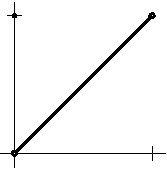
\includegraphics{figures/limvaldiff}
\caption{Function with a different limit and value at $0$.\label{fig:limvaldiff}}
\end{myfigureht}

Proof:  Let $\epsilon > 0$ be given.  Let $\delta \coloneqq \epsilon$.
For $x \in [0,1)$, $x \not= 0$, and $\abs{x-0} < \delta$, we get
\begin{equation*}
\abs{f(x) - 0} = \abs{x} < \delta = \epsilon .
\end{equation*}
\end{example}

\subsection{Sequential limits} \label{subseq:sequentiallimits}

Let us connect the limit as defined above with limits of sequences.

\begin{lemma}\label{seqflimit:lemma}
Let $S \subset \R$, let $c$ be a cluster point of $S$, let $f \colon S \to
\R$ be a function, and let $L \in \R$.

Then
$f(x) \to L$ as $x \to c$ if and only if for every sequence
$\{ x_n \}_{n=1}^\infty$
such that $x_n \in S \setminus \{c\}$ for all $n$,
and such that $\lim_{n\to\infty} x_n = c$,
we have that the sequence $\bigl\{ f(x_n) \bigr\}_{n=1}^\infty$ converges to $L$.
\end{lemma}

\begin{proof}
Suppose 
$f(x) \to L$ as $x \to c$, and $\{ x_n \}_{n=1}^\infty$ is a sequence
such that
$x_n \in S \setminus \{c\}$ and
$\lim_{n\to\infty} x_n = c$.
We wish to show that $\bigl\{ f(x_n) \bigr\}_{n=1}^\infty$ converges to $L$.
Let $\epsilon > 0$ be given.  Find a $\delta > 0$ such that
if $x \in S \setminus \{c\}$ and $\abs{x-c} < \delta$, then
$\abs{f(x) - L} < \epsilon$.  As
$\{ x_n \}_{n=1}^\infty$  converges to $c$, find an $M$ such that for $n \geq M$,
we have that $\abs{x_n - c} < \delta$.  Therefore, for $n \geq M$,
\begin{equation*}
\abs{f(x_n) - L} < \epsilon .
\end{equation*}
Thus $\bigl\{ f(x_n) \bigr\}_{n=1}^\infty$ converges to $L$.

For the other direction, we use proof by contrapositive.  Suppose 
it is not true that $f(x) \to L$ as $x \to c$.  The negation of the
definition is that there exists an $\epsilon > 0$ such that for every
$\delta > 0$ there exists an $x \in S \setminus \{c\}$, where
$\abs{x-c} < \delta$
and $\abs{f(x)-L} \geq \epsilon$.

Let us use $\nicefrac{1}{n}$ for $\delta$ in the statement above to
construct a sequence $\{ x_n \}_{n=1}^\infty$.  We have
that there exists an $\epsilon > 0$ such that for every $n$,
there exists a point $x_n \in S \setminus \{c\}$, where
$\abs{x_n-c} < \nicefrac{1}{n}$
and $\abs{f(x_n)-L} \geq \epsilon$.
The sequence $\{ x_n \}_{n=1}^\infty$ just constructed converges to $c$, but
the sequence $\bigl\{ f(x_n) \bigr\}_{n=1}^\infty$ does not converge to $L$.
And we are done.
\end{proof}

It is possible to strengthen the reverse direction of
the lemma by simply stating that
\myquote{$\bigl\{ f(x_n) \bigr\}_{n=1}^\infty$ converges,} without requiring a specific limit.
See \exerciseref{exercise:seqflimitalt}.

\begin{example}
$\displaystyle \lim_{x \to 0} \sin( \nicefrac{1}{x} )$
does not exist, but 
$\displaystyle \lim_{x \to 0} x\sin( \nicefrac{1}{x} ) = 0$.
See \figureref{figsin1x}.

\begin{myfigureht}
%left guy also used in 10.4
\subimport*{figures/}{sin1x_xsin1x.pdf_t}
\caption{Graphs of $\sin(\nicefrac{1}{x})$ and $x \sin(\nicefrac{1}{x})$.
Note that the computer cannot properly graph $\sin(\nicefrac{1}{x})$
near zero as it oscillates too fast.\label{figsin1x}}
\end{myfigureht}

Proof:
We start with $\sin(\nicefrac{1}{x})$.  Define a sequence
by
$x_n \coloneqq \frac{1}{\pi n + \nicefrac{\pi}{2}}$.  It is not hard to see
that $\lim_{n\to\infty} x_n = 0$.  Furthermore,
\begin{equation*}
\sin ( \nicefrac{1}{x_n} )
=
\sin (\pi n + \nicefrac{\pi}{2})
= {(-1)}^n .
\end{equation*}
Therefore, $\bigl\{ \sin ( \nicefrac{1}{x_n} ) \bigr\}_{n=1}^\infty$ does not converge.
By
\lemmaref{seqflimit:lemma}, 
$\displaystyle \lim_{x \to 0} \sin( \nicefrac{1}{x} )$ does not exist.

Now consider $x\sin(\nicefrac{1}{x})$.  Let $\{ x_n \}_{n=1}^\infty$ be a sequence
such that $x_n \not= 0$ for all $n$, and such that $\lim_{n\to\infty} x_n = 0$.
Notice that $\abs{\sin(t)} \leq 1$ for all $t \in \R$.  Therefore,
\begin{equation*}
\abs{x_n\sin(\nicefrac{1}{x_n})-0}
=
\abs{x_n}\abs{\sin(\nicefrac{1}{x_n})}
\leq
\abs{x_n} .
\end{equation*}
As $x_n$ goes to 0, then $\abs{x_n}$ goes to zero, and hence
$\bigl\{ x_n\sin(\nicefrac{1}{x_n}) \bigr\}_{n=1}^\infty$ converges to zero.  By
\lemmaref{seqflimit:lemma}, 
$\displaystyle \lim_{x \to 0} x\sin( \nicefrac{1}{x} ) = 0$.
\end{example}

Keep in mind the phrase \myquote{for every sequence} in the lemma.
For example, take $\sin(\nicefrac{1}{x})$ and the sequence given by
$x_n \coloneqq \nicefrac{1}{\pi n}$.
Then $\bigl\{ \sin (\nicefrac{1}{x_n}) \bigr\}_{n=1}^\infty$
is the constant zero sequence, and
therefore converges to zero, but the limit of 
$\sin(\nicefrac{1}{x})$ as $x \to 0$ does not exist.

Using \lemmaref{seqflimit:lemma}, 
we can start applying everything we know about
sequential limits to limits of functions.  Let us give a few important
examples.

\begin{cor}
Let $S \subset \R$ and let $c$ be a cluster point of $S$.  
Suppose $f \colon S \to
\R$ and $g \colon S \to \R$ are functions
such that
the limits of $f(x)$ and $g(x)$ as $x$ goes to $c$ both exist,
and
\begin{equation*}
f(x) \leq g(x) \qquad \text{for all } x \in S \setminus \{ c \}.
\end{equation*}
Then
\begin{equation*}
\lim_{x\to c} f(x) \leq \lim_{x\to c} g(x) .
\end{equation*}
\end{cor}

\begin{proof}
Take $\{ x_n \}_{n=1}^\infty$ be a sequence of numbers in $S \setminus \{ c \}$
that converges to $c$.  Let
\begin{equation*}
L_1 \coloneqq \lim_{x\to c} f(x), \qquad \text{and} \qquad L_2 \coloneqq \lim_{x\to c} g(x) .
\end{equation*}
\lemmaref{seqflimit:lemma} says that $\bigl\{ f(x_n) \bigr\}_{n=1}^\infty$ converges to
$L_1$ and $\bigl\{ g(x_n) \bigr\}_{n=1}^\infty$ converges to $L_2$.  We also
have $f(x_n) \leq g(x_n)$ for all $n$.
We obtain $L_1 \leq L_2$ using
\lemmaref{limandineq:lemma}.
\end{proof}

By applying constant functions, we get the following corollary.  The
proof is left as an exercise.

\begin{cor} \label{fconstineq:cor}
Let $S \subset \R$ and let $c$ be a cluster point of $S$.  Suppose $f \colon S \to
\R$ is a function such that the limit of $f(x)$ as $x$ goes to $c$
exists.
Suppose there are two real numbers $a$ and $b$ such that
\begin{equation*}
a \leq f(x) \leq b \qquad \text{for all } x \in S \setminus \{ c \}.
\end{equation*}
Then
\begin{equation*}
a \leq \lim_{x\to c} f(x) \leq b .
\end{equation*}
\end{cor}

Using \lemmaref{seqflimit:lemma} in the same way as above, we also get
the following corollaries, whose proofs are again left as exercises.

\begin{cor} \label{fsqueeze:cor}
Let $S \subset \R$ and let $c$ be a cluster point of $S$.
Suppose $f \colon S \to \R$,
$g \colon S \to \R$, and $h \colon S \to \R$ are functions such that
\begin{equation*}
f(x) \leq g(x) \leq h(x) \qquad \text{for all } x \in S \setminus \{ c \}.
\end{equation*}
Suppose the limits of $f(x)$ and $h(x)$ as $x$ goes to $c$ both exist, and
\begin{equation*}
\lim_{x\to c} f(x) = \lim_{x\to c} h(x) .
\end{equation*}
Then the limit of $g(x)$ as $x$ goes to $c$ exists and
\begin{equation*}
\lim_{x\to c} g(x) =
\lim_{x\to c} f(x) = \lim_{x\to c} h(x) .
\end{equation*}
\end{cor}

\begin{cor} \label{falg:cor}
Let $S \subset \R$ and let $c$ be a cluster point of $S$.  
Suppose $f \colon S \to \R$ and
$g \colon S \to \R$ are functions
such that 
the limits of $f(x)$ and $g(x)$ as $x$ goes to $c$ both exist.
Then
\begin{enumerate}[(i)]
\item
$\displaystyle
\lim_{x\to c} \bigl(f(x)+g(x)\bigr) = \left(\lim_{x\to c} f(x)\right) + 
\left(\lim_{x\to c} g(x)\right) .
$
\item
$\displaystyle
\lim_{x\to c} \bigl(f(x)-g(x)\bigr) = \left(\lim_{x\to c} f(x)\right) -
\left(\lim_{x\to c} g(x)\right) .
$
\item
$\displaystyle
\lim_{x\to c} \bigl(f(x)g(x)\bigr) = \left(\lim_{x\to c} f(x)\right)
\left(\lim_{x\to c} g(x)\right) .
$
\item \label{falg:cor:iv} If
$\displaystyle \lim_{x\to c} g(x) \not= 0$
and $g(x) \not= 0$ for all $x \in S \setminus \{ c \}$, then
\begin{equation*}
\lim_{x\to c} \frac{f(x)}{g(x)} =
\frac{\lim_{x\to c} f(x)}{\lim_{x\to c} g(x)} .
\end{equation*}
\end{enumerate}
\end{cor}

\begin{cor} \label{fabs:cor}
Let $S \subset \R$ and let $c$ be a cluster point of $S$.
Suppose $f \colon S \to \R$ is a function such that the limit of $f(x)$ as $x$ goes to $c$
exists.
Then
\begin{equation*}
\lim_{x\to c} \abs{f(x)} =
\abs{\lim_{x\to c} f(x)}.
\end{equation*}
\end{cor}

\subsection{Limits of restrictions and one-sided limits}

Sometimes we work with the function defined on a subset.

\begin{defn}
Let $f \colon S \to \R$ be a function and $A \subset S$.  Define the
function $f|_A \colon A \to \R$ by
\begin{equation*}
f|_A (x) \coloneqq f(x)  \qquad \text{for } x \in A.
\end{equation*}
We call $f|_A$ the \emph{\myindex{restriction}} of $f$ to $A$.
\end{defn}

The function $f|_A$ is simply the function $f$ taken on a smaller domain.
The following proposition is the analogue of taking a tail of a sequence.
It says that the limit is \myquote{local}: The limit only depends on points
arbitrarily near $c$.

\begin{prop} \label{prop:limrest}
Let $S \subset \R$, $c \in \R$, and
let $f \colon S
\to \R$ be a function.
Suppose
$A \subset S$ is such that there is some $\alpha > 0$ such that
$(A \setminus \{ c \}) \cap (c-\alpha,c+\alpha) = (S \setminus \{ c \}) \cap (c-\alpha,c+\alpha)$.
\begin{enumerate}[(i)]
\item The point $c$ is a cluster point of $A$ if and only if $c$ is a cluster point
of $S$.
\item Supposing $c$ is a cluster point of $S$, then $f(x) \to L$ as $x \to c$ if and only if
$f|_A(x) \to L$ as $x \to c$.
\end{enumerate}
\end{prop}

\begin{proof}
First, let $c$ be a cluster point of $A$.
Since $A \subset S$, then if $( A \setminus \{ c\} ) \cap
(c-\epsilon,c+\epsilon)$ is nonempty for every $\epsilon > 0$,
then $( S \setminus \{ c\} ) \cap
(c-\epsilon,c+\epsilon)$ is nonempty for every $\epsilon > 0$.
Thus $c$ is a cluster point of $S$.
Second, suppose $c$ is a cluster
point of $S$.  Then for $\epsilon > 0$ such that $\epsilon < \alpha$
we get that $( A \setminus \{ c\} ) \cap (c-\epsilon,c+\epsilon) =
( S \setminus \{ c\} ) \cap (c-\epsilon,c+\epsilon)$, which is nonempty.  This is true for all
$\epsilon < \alpha$ and hence 
$( A \setminus \{ c\} ) \cap (c-\epsilon,c+\epsilon)$ must be nonempty for all
$\epsilon > 0$.  Thus $c$ is a cluster point of $A$.

Now suppose $c$ is a cluster point of $S$ and $f(x) \to L$ as $x \to c$.  That is, for every $\epsilon > 0$
there is a $\delta > 0$ such that if $x \in S \setminus \{ c \}$
and $\abs{x-c} < \delta$, then $\abs{f(x)-L} < \epsilon$.  Because $A \subset S$,
if $x \in A \setminus \{ c \}$, then $x \in S \setminus \{ c \}$,
and hence $f|_A(x) \to L$ as $x \to c$.

Finally, suppose $f|_A(x) \to L$ as $x \to c$ and let $\epsilon > 0$ be
given.
There is a $\delta' > 0$ such that if $x \in A \setminus \{ c \}$
and $\abs{x-c} < \delta'$, then $\bigl\lvert f|_A(x)-L \bigr\rvert < \epsilon$.
Take $\delta \coloneqq \min \{ \delta', \alpha \}$.
Now suppose $x \in S \setminus \{ c \}$ and
$\abs{x-c} < \delta$.  As $\abs{x-c} < \alpha$, we find $x \in A \setminus \{ c \}$,
and as $\abs{x-c} < \delta'$, 
we get $\abs{f(x)-L} = \bigl\lvert f|_A(x)-L
\bigr\rvert < \epsilon$.
\end{proof}

The hypothesis on $A$ in the proposition is necessary.  For an arbitrary
restriction we generally get an implication in only one direction,
see \exerciseref{exercise:restrictionlimitexercise}.  
The usual notation for the limit is
\begin{equation*}
\lim_{\substack{x \to c\\x \in A}} f(x) \coloneqq \lim_{x \to c} f|_A(x) .
\end{equation*}
A common use of restriction with respect to limits, which does not satisfy
the hypothesis in the proposition, is the so-called
\emph{\myindex{one-sided limit}}%
\footnote{%
One sees a plethora of one-sided limit notations.
E.g.,
$\lim\limits_{\substack{x \to c\\x < c}} f(x)$,
$\lim\limits_{x \uparrow c} f(x)$, or
$\lim\limits_{x \nearrow c} f(x)$ for
$\lim\limits_{x \to c^-} f(x)$.}

\begin{defn} \label{defn:onesidedlimits}
Let $f \colon S \to \R$ be function and let $c \in \R$.  If
$c$ is a cluster point of
$S \cap (c,\infty)$
and the limit
of the restriction of $f$ to $S \cap (c,\infty)$ 
 as $x \to c$ exists, define
\glsadd{not:onesidedlim}
\begin{equation*}
\lim_{x \to c^+} f(x) \coloneqq \lim_{x\to c} f|_{S \cap (c,\infty)}(x) .
\end{equation*}
Similarly, if $c$ is a cluster point of 
$S \cap (-\infty,c)$ and the limit of the restriction as $x \to c$
exists, define
\begin{equation*}
\lim_{x \to c^-} f(x) \coloneqq \lim_{x\to c} f|_{S \cap (-\infty,c)}(x) .
\end{equation*}
\end{defn}

\propref{prop:limrest} does not apply to one-sided limits.
It is possible to have one-sided limits, but no limit at a point.  For
example, define $f \colon \R \to \R$ by $f(x) \coloneqq 1$ for $x < 0$ and
$f(x) \coloneqq 0$ for $x \geq 0$.
We leave it to the reader to verify that
\begin{equation*}
\lim_{x \to 0^-} f(x) = 1, \qquad
\lim_{x \to 0^+} f(x) = 0, \qquad
\lim_{x \to 0} f(x) \quad \text{does not exist.}
\end{equation*}
All is not lost, however, for we have the following replacement.

\begin{prop} \label{prop:onesidedlimits}
Let $S \subset \R$ be such that $c$ is a cluster point
of both $S \cap (-\infty,c)$ and $S \cap (c,\infty)$, let
$f \colon S \to \R$ be a function, and let $L \in \R$.  Then $c$ is a cluster point of $S$ and
\begin{equation*}
\lim_{x \to c} f(x) = L
\qquad \text{if and only if} \qquad
\lim_{x \to c^-} f(x) =
\lim_{x \to c^+} f(x) =
L .
\end{equation*}
\end{prop}

That is, a limit at $c$ exists if and only if both one-sided limits exist and are equal.  The
proof is a straightforward application of the definition of limit
and is left as an exercise.  The key point is that
$\bigl( S \cap (-\infty,c) \bigr) \cup \bigl( S \cap (c,\infty) \bigr)
= S \setminus \{ c \}$.

\subsection{Exercises}

\begin{exercise}
Find the limit (and prove it of course) or prove that the limit does not exist

\medskip

\noindent
\begin{tabular}{lllll}
a)
$\displaystyle
\lim_{x\to c} \sqrt{x}
$, for $c \geq 0$
& &
b)
$\displaystyle
\lim_{x\to c} x^2+x+1
$, for $c \in \R$
& &
c)
$\displaystyle
\lim_{x\to 0} x^2 \cos (\nicefrac{1}{x})
$
\\
d)
$\displaystyle
\lim_{x\to 0} \sin(\nicefrac{1}{x}) \cos (\nicefrac{1}{x})
$
& &
e)
$\displaystyle
\lim_{x\to 0} \sin(x) \cos (\nicefrac{1}{x})
$ & 
\end{tabular}
\end{exercise}

\begin{exercise}
Prove \corref{fconstineq:cor}.
\end{exercise}

\begin{exercise}
Prove \corref{fsqueeze:cor}.
\end{exercise}

\begin{exercise}
Prove \corref{falg:cor}.
\end{exercise}

\begin{exercise}
Let $A \subset S$.  Show that if $c$ is a cluster point of $A$, then $c$
is a cluster point of $S$.  Note the difference from
\propref{prop:limrest}.
\end{exercise}

\begin{exercise} \label{exercise:restrictionlimitexercise}
Let $A \subset S$.  Suppose $c$ is a cluster point of $A$ and
it is also a cluster point of $S$.
Let $f \colon S \to \R$ be a function.  Show that if
$f(x) \to L$ as $x \to c$, then
$f|_A(x) \to L$ as $x \to c$.
Note the difference from
\propref{prop:limrest}.
\end{exercise}

\begin{exercise}
Find an example of a function $f \colon [-1,1] \to \R$, where for
$A\coloneqq [0,1]$, we have
$f|_A(x) \to 0$ as $x \to 0$, but the limit of $f(x)$ as $x \to 0$
does not exist.  Note why you cannot apply
\propref{prop:limrest}.
\end{exercise}

\begin{exercise}
Find example functions $f$ and $g$ such that the limit of neither $f(x)$
nor $g(x)$ exists as $x \to 0$, but such that the limit of $f(x)+g(x)$ exists
as $x \to 0$.
\end{exercise}

\begin{exercise} \label{exercise:contlimitcomposition}
Let $c_1$ be a cluster point of $A \subset \R$ and $c_2$ be
a cluster point of $B \subset \R$.  Suppose 
$f \colon A \to B$ and $g \colon B \to \R$ are functions
such that
$f(x) \to c_2$ as $x \to c_1$ and
$g(y) \to L$ as $y \to c_2$.  If $c_2 \in B$, also suppose that $g(c_2) = L$.
Let $h(x) \coloneqq g\bigl(f(x)\bigr)$ and show
$h(x) \to L$ as $x \to c_1$.
Hint: Note that $f(x)$ could equal $c_2$ for many $x \in A$,
see also
\exerciseref{exercise:contlimitbadcomposition}.
\end{exercise}

%\begin{exercise}[note\footnote{This exercise is almost identical to the next one.  It
%will be replaced in the next major edition.}]
%Let $c$ be a cluster point of $A \subset \R$, and $f \colon A \to \R$
%be a function.  Suppose for every sequence $\{x_n\}_{n=1}^\infty$ in $A$,
%such that $\lim_{n\to\infty} x_n = c$,
%the sequence $\bigl\{ f(x_n) \bigr\}_{n=1}^\infty$ is Cauchy.  Prove that
%$\lim_{x\to c} f(x)$ exists.
%\end{exercise}
\begin{exercise}
Suppose that $f \colon \R \to \R$ be a function such that for every 
sequence $\{x_n\}_{n=1}^\infty$ in $\R$, the sequence
$\bigl\{ f(x_n) \bigr\}_{n=1}^\infty$ converges.  Prove that
$f$ is constant, that is,
$f(x) = f(y)$ for all $x,y \in \R$.
\end{exercise}

\begin{exercise} \label{exercise:seqflimitalt}
Prove the following stronger version of one direction of
\lemmaref{seqflimit:lemma}:
Let $S \subset \R$, $c$ be a cluster point of $S$, and $f \colon S \to
\R$ be a function.
Suppose that for every sequence $\{x_n\}_{n=1}^\infty$ in $S \setminus \{c\}$ such that
$\lim_{n\to\infty} x_n = c$ the sequence $\bigl\{ f(x_n) \bigr\}_{n=1}^\infty$ is convergent.
Then show that the limit of $f(x)$ as $x \to c$ exists.
\end{exercise}

\begin{exercise}
Prove \propref{prop:onesidedlimits}.
\end{exercise}

\begin{exercise}
Suppose $S \subset \R$ and $c$ is a cluster point of $S$.  Suppose $f \colon
S \to \R$ is bounded.  Show that there exists a sequence
$\{ x_n \}_{n=1}^\infty$
with $x_n \in S \setminus \{ c \}$ and $\lim_{n\to\infty} x_n = c$ such that
$\bigl\{ f(x_n) \bigr\}_{n=1}^\infty$ converges.
\end{exercise}

\begin{exercise}[Challenging] \label{exercise:contlimitbadcomposition}
Show that the hypothesis that $g(c_2) = L$ in
\exerciseref{exercise:contlimitcomposition} is necessary.  That is, find $f$
and $g$ such that $f(x) \to c_2$ as $x \to c_1$ and
$g(y) \to L$ as $y \to c_2$, but $g\bigl(f(x)\bigr)$ does not go to $L$
as $x \to c_1$.
\end{exercise}

\begin{exercise}
Show that the condition of being a cluster point is necessary to have a
reasonable definition of a limit.  That is, suppose $c$ is not a cluster
point of $S \subset \R$, and $f \colon S \to \R$ is a function.  Show that
every $L$ would satisfy the definition of limit at $c$ without the condition
on $c$ being a cluster point.
\end{exercise}

\begin{exercise}
\leavevmode
\begin{enumerate}[a)]
\item
Prove \corref{fabs:cor}.
\item
Find an example showing that the converse of
the corollary does not hold.
\end{enumerate}
\end{exercise}

%%%%%%%%%%%%%%%%%%%%%%%%%%%%%%%%%%%%%%%%%%%%%%%%%%%%%%%%%%%%%%%%%%%%%%%%%%%%%%

\sectionnewpage
\section{Continuous functions}
\label{sec:cont}

%mbxINTROSUBSECTION

\sectionnotes{2--2.5 lectures}

%You undoubtedly heard of continuous functions in your schooling.
A high-school criterion for the concept of continuity
is that a function is continuous if
we can draw its graph without lifting the pen from the paper.  While that
intuitive concept may be useful in simple situations, we require
rigor.  The following definition took three great mathematicians
(Bolzano, Cauchy, and finally Weierstrass) to get correctly and its final
form dates only to the late 1800s.

\subsection{Definition and basic properties}

\begin{defn}
Suppose $S \subset \R$ and $c \in S$.
We say $f \colon S \to \R$
is \emph{continuous at $c$}\index{continuous at $c$}
if for every $\epsilon > 0$
there is a $\delta > 0$ such that whenever $x \in S$ and $\abs{x-c} <
\delta$, we have
$\abs{f(x)-f(c)} < \epsilon$.

%\medskip

When $f \colon S \to \R$ is continuous at all $c \in S$, then we simply say
$f$ is a \emph{\myindex{continuous function}}\index{function!continuous}.
\end{defn}
\begin{myfigureht}
\subimport*{figures/}{contigr.pdf_t}
\caption{For $\abs{x-c} < \delta$, the graph of $f(x)$ should be within the gray region.\label{fig:contigr}}
\end{myfigureht}

If $f$ is continuous for all $c \in A$, we say
$f$ is \emph{continuous on $A \subset S$}.  A straightforward
exercise (\exerciseref{exercise:restrictioncontinuous})
shows that this implies that $f|_A$ is continuous, although
the converse does not hold (as we will see in \exampleref{example:removablediscont}).

Continuity may be the most important definition to understand in analysis,
and it is not an easy one.  See \figureref{fig:contigr}.
Note that $\delta$ not only
depends on $\epsilon$, but also on $c$;  we need not pick
one $\delta$ for all $c \in S$.
It is no accident 
that the definition of continuity is similar to the definition of a
limit of a function.  The main feature of continuous functions
is that these are precisely the functions that behave nicely with limits.

\begin{prop} \label{contbasic:prop}
Consider a function $f \colon S \to \R$ defined on a set  $S \subset \R$
and let $c \in S$.
Then:
%\begin{enumerate}[(i),itemsep=0.5\itemsep,parsep=0.5\parsep,topsep=0.5\topsep,partopsep=0.5\partopsep]
\begin{enumerate}[(i)]
\item \label{contbasic:prop:i}
If $c$ is not a cluster point of $S$, then $f$ is continuous at $c$.
\item \label{contbasic:prop:ii}
If $c$ is a cluster point of $S$, then $f$ is continuous at $c$
if and only if the limit of $f(x)$ as $x \to c$ exists and
\begin{equation*}
\lim_{x\to c} f(x) = f(c) .
\end{equation*}
\item \label{contbasic:prop:iii}
The function $f$ is continuous at $c$ if and only if for every sequence
$\{ x_n \}_{n=1}^\infty$
where $x_n \in S$ and $\lim\limits_{n\to\infty} x_n = c$, the sequence
$\bigl\{ f(x_n) \bigr\}_{n=1}^\infty$ converges
to $f(c)$.
\end{enumerate}
\end{prop}

\begin{proof}
\pagebreak[2]
We start with \ref{contbasic:prop:i}.  Suppose $c$ is not a cluster point of
$S$.  Then there exists a $\delta > 0$
such that $S \cap (c-\delta,c+\delta) = \{ c \}$.
For any $\epsilon > 0$, simply pick this given $\delta$.
The only $x \in S$ such that $\abs{x-c} < \delta$ is $x=c$.  Then
$\abs{f(x)-f(c)} = \abs{f(c)-f(c)} = 0 < \epsilon$.

Let us move to \ref{contbasic:prop:ii}.
Suppose $c$ is a cluster point of $S$.  Let us first suppose
that $\lim_{x\to c} f(x) = f(c)$.  Then for every $\epsilon > 0$,
there is a $\delta > 0$ such that if $x \in S \setminus \{ c \}$
and $\abs{x-c} < \delta$, then $\abs{f(x)-f(c)} < \epsilon$.
Also $\abs{f(c)-f(c)} = 0 < \epsilon$, so the definition of continuity at
$c$ is satisfied.  On the other hand, suppose $f$ is continuous
at $c$.  For every $\epsilon > 0$, there exists a $\delta > 0$
such that for $x \in S$ where $\abs{x-c} < \delta$, we have
$\abs{f(x)-f(c)} < \epsilon$.  Then the statement is, of course, still true if
$x \in S \setminus \{ c \} \subset S$.  Therefore, $\lim_{x\to c} f(x) =
f(c)$.

For \ref{contbasic:prop:iii}, first suppose $f$ is continuous at $c$.
Let $\{ x_n \}_{n=1}^\infty$
be a sequence such that $x_n \in S$ and $\lim_{n\to\infty} x_n = c$.  Let $\epsilon > 0$
be given.  Find a $\delta > 0$ such that $\abs{f(x)-f(c)} < \epsilon$
for all $x \in S$ where $\abs{x-c} < \delta$.  Find an $M \in \N$
such that for $n \geq M$, we have $\abs{x_n-c} < \delta$.  Then for
$n \geq M$, we have that $\abs{f(x_n)-f(c)} < \epsilon$,
so $\bigl\{ f(x_n) \bigr\}_{n=1}^\infty$
converges to $f(c)$.

We prove the other direction of \ref{contbasic:prop:iii} by contrapositive.
Suppose $f$ is not
continuous at $c$.  Then there exists an $\epsilon > 0$
such that for every $\delta > 0$, there exists an $x \in S$
such that $\abs{x-c} < \delta$ and $\abs{f(x)-f(c)} \geq \epsilon$.
Define a sequence $\{ x_n \}_{n=1}^\infty$ as follows.
Let $x_n \in S$ be such that $\abs{x_n-c} < \nicefrac{1}{n}$
and $\abs{f(x_n)-f(c)} \geq \epsilon$.
Now $\{ x_n \}_{n=1}^\infty$ is
a sequence in $S$ such that
$\lim_{n\to\infty} x_n = c$ and such that
$\abs{f(x_n)-f(c)} \geq \epsilon$ for all $n \in \N$.
Thus $\bigl\{ f(x_n) \bigr\}_{n=1}^\infty$
does not converge to $f(c)$.  It may or may not converge, but it definitely
does not converge to $f(c)$.  
\end{proof}

The last item in the proposition is particularly powerful.  It allows us to
quickly apply what we know about limits of sequences to continuous functions
and even to prove that certain functions are continuous.
It can also be strengthened, see \exerciseref{exercise:contseqalt}.

\begin{example}
The function $f \colon (0,\infty) \to \R$
defined by $f(x) \coloneqq \nicefrac{1}{x}$ is continuous.

Proof: Fix $c \in (0,\infty)$.  
Let $\{ x_n \}_{n=1}^\infty$ be a sequence in $(0,\infty)$ such that
$\lim_{n\to\infty} x_n = c$.  Then
\begin{equation*}
f(c) = \frac{1}{c}
=
\frac{1}{\lim_{n\to\infty} x_n}
=
\lim_{n \to \infty} \frac{1}{x_n}
=
\lim_{n \to \infty} f(x_n) .
\end{equation*}
Thus $f$ is continuous at $c$.  As $f$ is continuous at all $c \in
(0,\infty)$, $f$ is continuous.
\end{example}

We have previously shown $\lim_{x \to c} x^2 = c^2$ directly.  Therefore
the function $x^2$ is continuous.  The last item of \propref{contbasic:prop} and the continuity of
algebraic operations with respect to limits of sequences,
\propref{prop:contalg}, gives a quick proof of a much more general result.

\begin{prop}
Let $f \colon \R \to \R$ be a \emph{\myindex{polynomial}}.  That is,
\begin{equation*}
f(x) = a_d x^d + a_{d-1} x^{d-1} + \cdots + a_1 x + a_0 ,
\end{equation*}
for some constants $a_0, a_1, \ldots, a_d$.
Then $f$ is continuous.
\end{prop}

\begin{proof}
Fix $c \in \R$.  
Let $\{ x_n \}_{n=1}^\infty$ be a sequence such that
$\lim_{n\to\infty} x_n = c$.  Then
\begin{equation*}
\begin{split}
f(c) &=
a_d c^d + a_{d-1} c^{d-1} + \cdots + a_1 c + a_0 
\\
&= 
a_d {\left(\lim_{n\to\infty} x_n\right)}^d
+ a_{d-1} {\left(\lim_{n\to\infty} x_n\right)}^{d-1}
+ \cdots
+ a_1 \left(\lim_{n\to\infty} x_n\right) + a_0 
\\
& =
\lim_{n \to \infty}
\left(
a_d x_n^d + a_{d-1} x_n^{d-1} + \cdots + a_1 x_n + a_0 
\right)
=
\lim_{n \to \infty}
f(x_n) .
\avoidbreak
\end{split}
\end{equation*}
Thus $f$ is continuous at $c$.  As $f$ is continuous at all $c \in \R$,
$f$ is continuous.
\end{proof}

By similar reasoning, or by appealing to \corref{falg:cor},
we can prove the following proposition.  The proof is left as an
exercise.

\begin{prop} \label{contalg:prop}
Let $f \colon S \to \R$ and $g \colon S \to \R$ be functions
continuous at $c \in S$.
\begin{enumerate}[(i)]
\item The function $h \colon S \to \R$ defined by
$h(x) \coloneqq f(x)+g(x)$ is continuous at $c$.
\item The function $h \colon S \to \R$ defined by
$h(x) \coloneqq f(x)-g(x)$ is continuous at $c$.
\item The function $h \colon S \to \R$ defined by
$h(x) \coloneqq f(x)g(x)$ is continuous at $c$.
\item If $g(x)\not=0$ for all $x \in S$, the function $h \colon S \to \R$
given by $h(x) \coloneqq \frac{f(x)}{g(x)}$ is continuous at $c$.
\end{enumerate}
\end{prop}

\begin{example} \label{sincos:example}
The functions $\sin(x)$ and $\cos(x)$ are continuous.
In the following computations we use the sum-to-product
trigonometric identities.  We also use the simple facts that
$\abs{\sin(x)} \leq \abs{x}$, $\abs{\cos(x)} \leq 1$,
and $\abs{\sin(x)} \leq 1$.
\begin{equation*}
\begin{split}
\abs{\sin(x)-\sin(c)} & =
\abs{
2 \sin \left( \frac{x-c}{2} \right) \cos \left( \frac{x+c}{2} \right)
}
\\
& =
2
\abs{ \sin \left( \frac{x-c}{2} \right) }
\abs{ \cos \left( \frac{x+c}{2} \right) }
\\
& \leq
2
\abs{ \sin \left( \frac{x-c}{2} \right) }
\\
& \leq
2
\abs{ \frac{x-c}{2} }
= \abs{x-c}
\end{split}
\end{equation*}
\begin{equation*}
\begin{split}
\abs{\cos(x)-\cos(c)} & =
\abs{
-2 \sin \left( \frac{x-c}{2} \right) \sin \left( \frac{x+c}{2} \right)
}
\\
& =
2
\abs{ \sin \left( \frac{x-c}{2} \right) }
\abs{ \sin \left( \frac{x+c}{2} \right) }
\\
& \leq
2
\abs{ \sin \left( \frac{x-c}{2} \right) }
\\
& \leq
2
\abs{ \frac{x-c}{2} }
= \abs{x-c}
\end{split}
\end{equation*}

The claim that $\sin$ and $\cos$ are continuous follows by taking an
arbitrary sequence $\{ x_n \}_{n=1}^\infty$ converging to $c$, or by applying the
definition of continuity directly.  Details are left to the
reader.
\end{example}

\subsection{Composition of continuous functions}

You probably already realized that one of the basic tools in
constructing complicated functions out of simple ones is composition.
Recall that for two functions $f$ and $g$,
the composition $f \circ g$ is defined by
$(f \circ g)(x) \coloneqq f\bigl(g(x)\bigr)$.
A composition of
continuous functions is again
continuous.

\begin{prop} \label{prop:compositioncont}
Let $A, B \subset \R$ and $f \colon B \to \R$ and $g \colon A \to B$ be
functions.  If $g$ is continuous at $c \in A$ and
$f$ is continuous at $g(c)$, then $f \circ g \colon A \to \R$ is continuous
at $c$.
\end{prop}

\begin{proof}
Let $\{ x_n \}_{n=1}^\infty$ be a sequence in $A$ such that
$\lim_{n\to\infty} x_n = c$.
As $g$ is continuous at $c$, we have $\bigl\{ g(x_n) \bigr\}_{n=1}^\infty$ converges to $g(c)$.
As $f$ is continuous at $g(c)$, we have $\bigl\{ f\bigl(g(x_n)\bigr)
\bigr\}_{n=1}^\infty$ converges
to $f\bigl(g(c)\bigr)$.
Thus $f \circ g$ is continuous at $c$.
\end{proof}

\begin{example}
Claim: \emph{${\bigl(\sin(\nicefrac{1}{x})\bigr)}^2$ is a continuous
function on $(0,\infty)$.}

Proof: The function $\nicefrac{1}{x}$ is continuous on
$(0,\infty)$ and $\sin(x)$ is continuous on $(0,\infty)$ (actually
on $\R$, but $(0,\infty)$ is the range for $\nicefrac{1}{x}$).
Hence the composition $\sin(\nicefrac{1}{x})$ is continuous.  Also,
$x^2$ is continuous on the interval $[-1,1]$ (the range of $\sin$).  Thus
the composition
${\bigl(\sin(\nicefrac{1}{x})\bigr)}^2$ is continuous on $(0,\infty)$.
\end{example}

\subsection{Discontinuous functions}

When $f$ is not continuous at $c$, we
say $f$ is \emph{\myindex{discontinuous}} at $c$, or that it has a
\emph{\myindex{discontinuity}} at~$c$.
The following proposition is a useful test and follows immediately
from third item of \propref{contbasic:prop}.

\begin{prop}
Let $f \colon S \to \R$ be a function and $c \in S$.  Suppose 
there exists a sequence $\{ x_n \}_{n=1}^\infty$, $x_n \in S$ for all $n$,
and $\lim_{n\to\infty} x_n = c$
such that $\bigl\{ f(x_n) \bigr\}_{n=1}^\infty$
does not converge to $f(c)$.
Then $f$ is discontinuous at $c$.
\end{prop}

Again, 
saying that 
$\bigl\{ f(x_n) \bigr\}_{n=1}^\infty$ does not converge to $f(c)$
means that it
either does not converge
at all, or it converges to something
other than $f(c)$.

\begin{example} \label{example:jumpdiscont}
The function $f \colon \R \to \R$ defined by
\begin{equation*}
f(x) \coloneqq 
\begin{cases}
-1 & \text{if } x < 0, \\
1 & \text{if } x \geq 0
\end{cases}
\end{equation*}
is not continuous at 0.

Proof: Consider $\{ \nicefrac{-1}{n} \}_{n=1}^\infty$, which converges to 0.  Then
$f(\nicefrac{-1}{n}) = -1$ for every $n$,
and so
$\lim_{n\to\infty} f(\nicefrac{-1}{n}) = -1$, but $f(0) = 1$.  Thus the function is
not continuous at 0.  See
\figureref{fig:jumpdiscont}.

\begin{myfigureht}
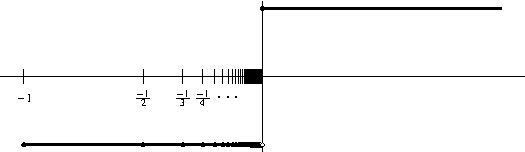
\includegraphics{figures/jumpdiscont}
\caption{Jump discontinuity.  The values of
$f(\nicefrac{-1}{n})$ and $f(0)$ are marked as black dots.\label{fig:jumpdiscont}}
\end{myfigureht}

Notice that $f(\nicefrac{1}{n}) = 1$ for all $n \in \N$.
Hence, $\lim_{n\to\infty} f(\nicefrac{1}{n}) = f(0) = 1$.  So
$\bigl\{ f(x_n) \bigr\}_{n=1}^\infty$ may converge to $f(0)$
for some specific
sequence $\{ x_n \}_{n=1}^\infty$ going to 0,
despite the function being discontinuous at 0.

Finally, consider $f\Bigl(\frac{{(-1)}^n}{n}\Bigr) = {(-1)}^n$.
This sequence diverges.
\end{example}

\begin{example}
For an extreme example, take the so-called
\emph{\myindex{Dirichlet function}}\footnote{Named after the German
mathematician
\href{https://en.wikipedia.org/wiki/Peter_Gustav_Lejeune_Dirichlet}{Johann Peter Gustav Lejeune
Dirichlet}
(1805--1859).}.
\begin{equation*}
f(x) \coloneqq
\begin{cases}
1 & \text{if } x \text{ is rational,} \\
0 & \text{if } x \text{ is irrational.}
\end{cases}
\avoidbreak
\end{equation*}
The function $f$ is discontinuous at all $c \in \R$.

Proof:
If $c$ is rational, take a sequence $\{ x_n \}_{n=1}^\infty$
of irrational numbers such that $\lim_{n\to\infty} x_n = c$ (why can we?).  Then $f(x_n) = 0$
and so $\lim_{n\to\infty} f(x_n) = 0$, but $f(c) = 1$.
If $c$ is irrational, take a sequence of rational numbers
$\{ x_n \}_{n=1}^\infty$
that converges to $c$ (why can we?).  Then $\lim_{n\to\infty} f(x_n) = 1$, but $f(c) = 0$.
\end{example}

Let us test the limits of our intuition.  Can
there exist a function continuous at all irrational numbers, but
discontinuous at all rational numbers?  There are rational numbers
arbitrarily close to any irrational number.  Perhaps strangely, the
answer is yes, such a function exists.  The following example is called the
\emph{\myindex{Thomae function}}\footnote{Named after the German
mathematician
\href{https://en.wikipedia.org/wiki/Carl_Johannes_Thomae}{Carl Johannes Thomae}
(1840--1921).} or the
\emph{\myindex{popcorn function}}.

\begin{example} \label{popcornfunction:example}
Define $f \colon (0,1) \to \R$ as
\begin{equation*}
f(x) \coloneqq 
\begin{cases}
\nicefrac{1}{k} & \text{if } x=\nicefrac{m}{k}, \text{ where } m,k \in \N
\text{ and have no common divisors (lowest terms),} \\
0 & \text{if } x \text{ is irrational.}
\end{cases}
\end{equation*}
See the graph of $f$
in \figureref{popcornfig}.
We claim that
$f$ is continuous at all irrational $c$ and 
discontinuous at all rational $c$.
\begin{myfigureht}
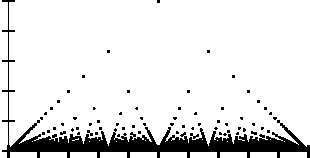
\includegraphics{figures/popcornfig}
\caption{Graph of the \myquote{popcorn function.}\label{popcornfig}}
\end{myfigureht}

Proof:
Let $c = \nicefrac{m}{k}$ be rational and in lowest terms.  Take a sequence of
irrational numbers $\{ x_n \}_{n=1}^\infty$ such that $\lim_{n\to\infty} x_n = c$.  Then
$\lim_{n\to\infty} f(x_n) = \lim_{n\to\infty} 0 = 0$, but $f(c) = \nicefrac{1}{k} \not= 0$.  So $f$
is discontinuous at $c$.

Now let $c$ be irrational, so $f(c) = 0$.  Take a sequence 
$\{ x_n \}_{n=1}^\infty$ in $(0,1)$ such that $\lim_{n\to\infty} x_n = c$.
Given $\epsilon > 0$, find $K \in \N$ such
that $\nicefrac{1}{K} < \epsilon$
by the \hyperref[thm:arch:i]{Archimedean property}.
If $\nicefrac{m}{k} \in (0,1)$ and $m,k \in \N$, then $0 < m < k$.
So there are only finitely many rational numbers in $(0,1)$
whose denominator $k$ in lowest terms is less than $K$.
As $\lim_{n\to\infty} x_n = c$, every number not equal to $c$ can appear at most
finitely many times in $\{ x_n \}_{n=1}^\infty$.
Hence,
there is an $M$ such that for $n \geq M$, all the numbers $x_n$
that are rational
have a denominator larger than or equal to $K$.  Thus for $n \geq M$,
\begin{equation*}
\abs{f(x_n) - 0} = f(x_n) \leq \nicefrac{1}{K} < \epsilon .
\end{equation*}
Therefore, $f$ is continuous at irrational $c$.
\end{example}

Let us end on an easier example.

\begin{example} \label{example:removablediscont}
Define
$g \colon \R \to \R$ by $g(x) \coloneqq 0$ if $x \not= 0$ and
$g(0) \coloneqq 1$.  Then $g$ is not continuous at zero, but continuous everywhere else (why?).
The point $x=0$ is called a \emph{\myindex{removable discontinuity}}.  That
is because if we would change the definition of $g$, by insisting that
$g(0)$ be $0$, we would obtain a continuous function.  On the other hand,
let $f$ be the function of \exampleref{example:jumpdiscont}.
Then $f$ does not have a
removable discontinuity at $0$.  No matter how we would define $f(0)$ the function
would still fail to be continuous.  The difference is that 
$\lim_{x\to 0} g(x)$ exists while
$\lim_{x\to 0} f(x)$ does not.

We stay with this example to show another phenomenon.
Let $A \coloneqq \{ 0 \}$, then $g|_A$ is continuous (why?), while $g$ is not continuous on $A$.
Similarly, if $B \coloneqq \R \setminus \{0 \}$, then $g|_B$ is also continuous,
and $g$ is in fact continuous on $B$.
\end{example}

\subsection{Exercises}

\begin{exercise}
Using the definition of continuity directly prove that
$f \colon \R \to \R$ defined by
$f(x) \coloneqq x^2$ is continuous.
\end{exercise}

\begin{exercise}
Using the definition of continuity directly prove that
$f \colon (0,\infty) \to \R$ defined by
$f(x) \coloneqq \nicefrac{1}{x}$ is continuous.
\end{exercise}

\begin{exercise}
Define $f \colon \R \to \R$ by
\begin{equation*}
f(x) \coloneqq
\begin{cases}
x & \text{if } x \text{ is rational,} \\
x^2 & \text{if } x \text{ is irrational.}
\end{cases}
\avoidbreak
\end{equation*}
Using the definition of continuity directly prove that
$f$ is continuous at $1$ and discontinuous at $2$.
\end{exercise}

\begin{exercise}
Define $f \colon \R \to \R$ by
\begin{equation*}
f(x) \coloneqq
\begin{cases}
\sin(\nicefrac{1}{x}) & \text{if } x \not= 0, \\
0 & \text{if } x=0.
\end{cases}
\avoidbreak
\end{equation*}
Is $f$ continuous?  Prove your assertion.
\end{exercise}

\begin{exercise}
Define $f \colon \R \to \R$ by
\begin{equation*}
f(x) \coloneqq
\begin{cases}
x \sin(\nicefrac{1}{x}) & \text{if } x \not= 0, \\
0 & \text{if } x=0.
\end{cases}
\avoidbreak
\end{equation*}
Is $f$ continuous?  Prove your assertion.
\end{exercise}

\begin{exercise}
Prove \propref{contalg:prop}.
\end{exercise}

\begin{exercise} \label{exercise:restrictioncontinuous}
Let $S \subset \R$ and $A \subset S$.  Let $f \colon S \to \R$
be a continuous function.
Prove that the restriction $f|_A$ is continuous.
\end{exercise}

\begin{exercise}
Suppose $S \subset \R$, such that $(c-\alpha,c+\alpha) \subset S$ for some $c \in \R$
and $\alpha > 0$.
Let $f \colon S \to \R$ be a function and $A \coloneqq (c-\alpha,c+\alpha)$.  Prove that
if $f|_A$ is continuous at $c$, then $f$ is continuous at $c$.
\end{exercise}

\begin{exercise}
Give an example of functions $f \colon \R \to \R$ and $g \colon \R \to \R$
such that the function $h$, defined by $h(x) \coloneqq f(x) + g(x)$, is continuous,
but $f$ and $g$ are not continuous.  Can you find $f$ and $g$ that are nowhere
continuous, but $h$ is a continuous function?
\end{exercise}

\begin{exercise}
Let $f \colon \R \to \R$ and 
$g \colon \R \to \R$ be continuous functions.  Suppose that
$f(r) = g(r)$ for all $r \in \Q$.
Show that $f(x) = g(x)$ for all $x \in \R$.
\end{exercise}

\begin{exercise} \label{exercise:positivecontneigh}
Let $f \colon \R \to \R$ be continuous.  Suppose $f(c) > 0$.  Show that
there exists an $\alpha > 0$ such that for all $x \in (c-\alpha,c+\alpha)$,
we have $f(x) > 0$.
\end{exercise}

\begin{exercise}
Let $f \colon \Z \to \R$ be a function.  Show that $f$ is continuous.
\end{exercise}

\begin{exercise} \label{exercise:contseqalt}
Let $f \colon S \to \R$ be a function and $c \in S$, such that for every
sequence $\{ x_n \}_{n=1}^\infty$ in $S$ with $\lim_{n\to\infty} x_n = c$, the sequence
$\bigl\{ f(x_n) \bigr\}_{n=1}^\infty$ converges.  Show that $f$ is continuous at $c$.
\end{exercise}

\begin{exercise}
Suppose $f \colon [-1,0] \to \R$ and $g \colon [0,1] \to \R$ are continuous
and $f(0) = g(0)$.  Define $h \colon [-1,1] \to \R$ by 
$h(x) \coloneqq f(x)$ if $x \leq 0$ and $h(x) \coloneqq g(x)$ if $x > 0$.  Show that
$h$ is continuous.
\end{exercise}

\begin{exercise}
Suppose $g \colon \R \to \R$ is a continuous function such that $g(0) = 0$,
and suppose $f \colon \R \to \R$ is such that
$\abs{f(x)-f(y)} \leq g(x-y)$ for all $x$ and $y$.  Show that $f$ is
continuous.
\end{exercise}

\begin{exercise}[Challenging]
Suppose $f \colon \R \to \R$ is continuous at $0$ and
such that $f(x+y) = f(x) + f(y)$ for every $x$ and $y$.
Show that $f(x) = ax$ for some $a \in \R$.
Hint: Show that $f(nx) = nf(x)$, then show $f$ is continuous on $\R$.
Then show that $\nicefrac{f(x)}{x} = f(1)$ for all rational $x$.
\end{exercise}

\begin{exercise} \label{exercise:minmaxcont}
Suppose $S \subset \R$ and
let $f \colon S \to \R$ and
$g \colon S \to \R$ be continuous functions.
Define $p \colon S \to \R$ by
$p(x) \coloneqq \max \bigl\{ f(x) , g(x) \bigr\}$ and
$q \colon S \to \R$ by
$q(x) \coloneqq \min \bigl\{ f(x) , g(x) \bigr\}$.  Prove that $p$ and $q$ are
continuous.
\end{exercise}

\begin{exercise}
Suppose $f \colon [-1,1] \to \R$ is a function continuous at all $x \in
[-1,1] \setminus \{ 0 \}$.  Show that for every $\epsilon$ such
that $0 < \epsilon < 1$, there exists
a function $g \colon [-1,1] \to \R$ continuous on all of $[-1,1]$, such that
$f(x) = g(x)$ for all $x \in [-1,-\epsilon] \cup [\epsilon,1]$, and 
$\abs{g(x)} \leq \abs{f(x)}$ for all $x \in [-1,1]$.
\end{exercise}

\begin{exercise}[Challenging]
A function $f \colon I \to \R$ is \emph{\myindex{convex}} if
whenever $a \leq x \leq b$ for $a,x,b$ in $I$, we have
$f(x) \leq f(a) \frac{b-x}{b-a} + f(b) \frac{x-a}{b-a}$.  In other words,
if the line drawn between $\bigl(a,f(a)\bigr)$ and $\bigl(b,f(b)\bigr)$ 
is above the graph of $f$.
\begin{enumerate}[a)]
\item
Prove that
if $I = (\alpha,\beta)$ an open interval and $f \colon I \to \R$ is convex,
then $f$ is continuous.
\item
Find an example of a convex $f \colon [0,1] \to \R$ that is
not continuous.
\end{enumerate}
\end{exercise}


%%%%%%%%%%%%%%%%%%%%%%%%%%%%%%%%%%%%%%%%%%%%%%%%%%%%%%%%%%%%%%%%%%%%%%%%%%%%%%

\sectionnewpage
\section{Extreme and intermediate value theorems}
\label{sec:minmaxint}

%mbxINTROSUBSECTION

\sectionnotes{1.5 lectures}

Continuous functions on closed and bounded intervals
are quite well behaved.

\subsection{Min-max or extreme value theorem}

Recall that $f \colon [a,b] \to \R$ is
\emph{bounded}\index{bounded function}\index{function!bounded}
if there exists a $B \in \R$ such that
$\abs{f(x)} \leq B$ for all $x \in [a,b]$.
For a continuous function on a closed and bounded interval, we have the following lemma.

\begin{lemma}
A continuous function $f \colon [a,b] \to \R$ is bounded.
\end{lemma}

\begin{proof}
We prove the claim by contrapositive.  Suppose $f$ is not bounded.
Then for each
$n \in \N$, there is an $x_n \in [a,b]$, such that
\begin{equation*}
\abs{f(x_n)} \geq n .
\end{equation*}
The sequence $\{ x_n \}_{n=1}^\infty$ is bounded as $a \leq x_n \leq b$.
By the \hyperref[thm:bwseq]{Bolzano--Weierstrass theorem},
there is a convergent subsequence $\{ x_{n_i} \}_{i=1}^\infty$.
Let $x \coloneqq \lim_{i\to\infty} x_{n_i}$.
Since $a \leq x_{n_i} \leq b$ for all $i$, then $a \leq x \leq b$.
The sequence $\bigl\{ f(x_{n_i}) \bigr\}_{i=1}^\infty$ is not bounded 
as 
$\abs{f(x_{n_i})} \geq n_i \geq i$.
Thus $f$ is not continuous at $x$ as
\begin{equation*}
f(x)
=
f\Bigl( \lim_{i\to\infty} x_{n_i} \Bigr) ,
\qquad \text{but} \qquad
\lim_{i\to\infty} f(x_{n_i}) \enspace \text{does not exist.} \qedhere
\end{equation*}
\end{proof}

Notice a key point of the proof.
Boundedness of $[a,b]$ allows us to use Bolzano--Weierstrass,
while the fact that it is closed gives us that the limit is back in $[a,b]$.
The technique is a common one: Find a sequence with a certain property,
then use Bolzano--Weierstrass to make such a sequence that also converges.

Recall from calculus that $f \colon S \to \R$ achieves an
\emph{\myindex{absolute minimum}}\index{minimum!absolute}%
\index{achieves absolute minimum}
at $c \in S$ if
\begin{equation*}
f(x) \geq f(c) \qquad \text{for all } x \in S.
\end{equation*}
On the other hand, $f$ achieves an 
\emph{\myindex{absolute maximum}}\index{maximum!absolute}%
\index{achieves absolute maximum}
at $c \in S$ if
\begin{equation*}
f(x) \leq f(c) \qquad \text{for all } x \in S.
\end{equation*}
If such a $c \in S$ exists, then we say
$f$ \emph{achieves an absolute minimum (resp.\ absolute maximum) on
$S$}, and we call
$f(c)$ the \emph{absolute minimum (resp.\ absolute maximum)}.
%See \figureref{fig:minmax}.
\begin{myfigureht}
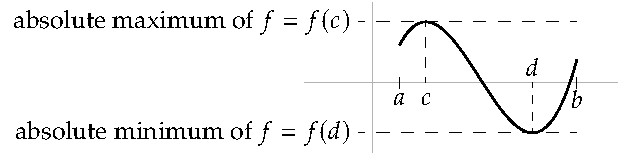
\includegraphics{figures/minmax}
\caption{$f \colon [a,b] \to \R$ achieves an absolute maximum $f(c)$ at
$c$, and an absolute minimum $f(d)$ at $d$.\label{fig:minmax}}
\end{myfigureht}

If $S$ is a closed
and bounded interval, then a continuous $f$
is not just bounded, it must achieve an absolute minimum and an absolute
maximum on $S$.

\begin{thm}[Minimum-maximum theorem / Extreme value theorem]
\index{minimum-maximum theorem}%
\index{maximum-minimum theorem}%
\index{extreme value theorem}%
A continuous function $f \colon [a,b] \to \R$
achieves both an absolute minimum and an absolute maximum on $[a,b]$.
\end{thm}

Again, we remark that is important that the domain of $f$ is a closed and bounded interval $[a,b]$.

\begin{proof}
The lemma says that $f$ is bounded, so
the set $f\bigl([a,b]\bigr) = \bigl\{ f(x) : x \in [a,b] \bigr\}$ has a supremum and an infimum.
There exist sequences
in the set $f\bigl([a,b]\bigr)$ that approach its supremum and its infimum.
That is, there are sequences
$\bigl\{ f(x_n) \bigr\}_{n=1}^\infty$ and $\bigl\{ f(y_n)
\bigr\}_{n=1}^\infty$, where $x_n$ and $y_n$ are in $[a,b]$,
such that
\begin{equation*}
\lim_{n\to\infty} f(x_n) = \inf f\bigl([a,b]\bigr) \qquad \text{and} \qquad
\lim_{n\to\infty} f(y_n) = \sup f\bigl([a,b]\bigr).
\end{equation*}
We are not done yet; we need to find where the minima and the maxima are.
The problem is that the sequences $\{ x_n \}_{n=1}^\infty$ and
$\{ y_n \}_{n=1}^\infty$ need not converge.
We know $\{ x_n \}_{n=1}^\infty$ and $\{ y_n \}_{n=1}^\infty$ are bounded
(their elements belong to a bounded interval $[a,b]$).
Apply the 
\hyperref[thm:bwseq]{Bolzano--Weierstrass theorem}
to find
convergent subsequences
$\{ x_{n_i} \}_{i=1}^\infty$ and 
$\{ y_{m_i} \}_{i=1}^\infty$.  Let
\begin{equation*}
x \coloneqq \lim_{i\to\infty} x_{n_i}
\qquad \text{and} \qquad
y \coloneqq \lim_{i\to\infty} y_{m_i}.
\end{equation*}
As $a \leq x_{n_i} \leq b$ for all $i$, we have $a \leq x \leq b$.
Similarly, $a \leq y \leq b$.  So $x$ and $y$ are in $[a,b]$.
A limit of a subsequence is the same as the limit of the
sequence, and we can take a limit past the continuous function $f$:
\begin{equation*}
\inf f\bigl([a,b]\bigr) = \lim_{n\to\infty} f(x_n)
= \lim_{i\to\infty} f(x_{n_i}) = 
f \Bigl( \lim_{i\to\infty} x_{n_i} \Bigr) = f(x) .
\end{equation*}
Similarly,
\begin{equation*}
\sup f\bigl([a,b]\bigr) = \lim_{n\to\infty} f(y_n)
= \lim_{i\to\infty} f(y_{m_i}) = 
f \Bigl( \lim_{i\to\infty} y_{m_i} \Bigr) = f(y) .
\end{equation*}
Hence, $f$ achieves an absolute minimum at $x$ and
an absolute maximum at $y$.
\end{proof}

\begin{example}
The function $f(x) \coloneqq x^2+1$ defined on the interval $[-1,2]$ achieves a minimum
at $x=0$ when $f(0) = 1$.  It achieves a maximum at $x=2$ where $f(2) = 5$.
Do note that the domain of definition matters.  If we instead took the domain
to be $[-10,10]$, then $f$ would no longer have a maximum at $x=2$.
Instead,
the maximum would be achieved at either $x=10$ or $x=-10$.
\end{example}

We show by examples that the different hypotheses of the theorem are
truly needed.

\begin{example}
The function $f \colon \R \to \R$ defined by $f(x) \coloneqq x$
achieves neither a minimum, nor a maximum.  So it is important that
we are looking at a bounded interval.
\end{example}

\begin{example}
The function $f \colon (0,1) \to \R$ defined by $f(x) \coloneqq \nicefrac{1}{x}$
achieves neither a minimum, nor a maximum.
It is continuous, but $(0,1)$ is not closed.
The values of the function are
unbounded as we approach $0$.  Also as we approach $x=1$, the values of the
function approach $1$, but $f(x) > 1$ for all $x \in (0,1)$.  There is
no $x \in (0,1)$ such that $f(x) = 1$.  So it is important that
we are looking at a closed interval.
\end{example}

\begin{example}
Continuity is important.
Define $f \colon [0,1] \to \R$ by 
$f(x) \coloneqq \nicefrac{1}{x}$ for $x > 0$ and let $f(0) \coloneqq 0$.
The function does not achieve a maximum.  The domain $[0,1]$ is closed and
bounded, but the problem is that
the function is not continuous at 0.
\end{example}

\subsection{Bolzano's intermediate value theorem}

Bolzano's intermediate value theorem is one of the cornerstones of analysis.
It is sometimes only called the intermediate value theorem, or just
Bolzano's theorem.  To prove Bolzano's theorem we prove the
following simpler lemma.

\begin{lemma} \label{IVT:lemma}
Let $f \colon [a,b] \to \R$ be a continuous function.
Suppose $f(a) < 0$ and $f(b) > 0$. 
Then there exists a number $c \in (a,b)$
such that $f(c) = 0$.
\end{lemma}

\begin{proof}
We define two sequences $\{ a_n \}_{n=1}^\infty$
and $\{ b_n \}_{n=1}^\infty$ inductively:
\begin{enumerate}[(i)]
\item Let $a_1 \coloneqq a$ and $b_1 \coloneqq b$.
\item If $f\left(\frac{a_n+b_n}{2}\right) \geq 0$, let $a_{n+1} \coloneqq a_n$ and
$b_{n+1} \coloneqq \frac{a_n+b_n}{2}$.
\item If $f\left(\frac{a_n+b_n}{2}\right) < 0$, let $a_{n+1} \coloneqq \frac{a_n+b_n}{2}$ and
$b_{n+1} \coloneqq b_n$.
\end{enumerate}
\begin{myfigureht}
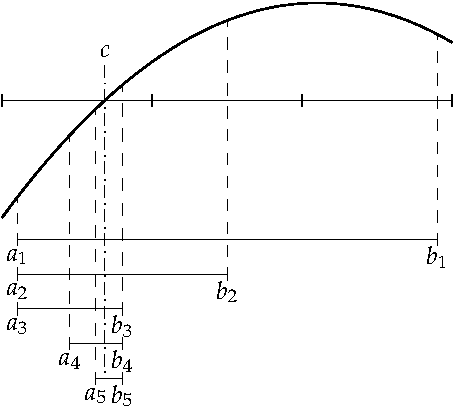
\includegraphics{figures/bisect}
\caption{Finding roots (bisection method).\label{bisectfig}}
\end{myfigureht}
See \figureref{bisectfig} for an example defining the first five steps.
If $a_n < b_n$, then $a_n < \frac{a_n+b_n}{2} < b_n$.  So
$a_{n+1} < b_{n+1}$.
Thus by \hyperref[induction:thm]{induction} $a_n < b_n$ for all $n$.
Furthermore, $a_n \leq a_{n+1}$ and 
$b_n \geq b_{n+1}$ for all $n$, that is, the sequences are monotone.
As $a_n < b_n \leq b_1 = b$ and 
$b_n > a_n \geq a_1 = a$ for all $n$,
the sequences are also bounded.  Therefore, the
sequences converge.
Let $c \coloneqq \lim_{n\to\infty} a_n$ and $d \coloneqq \lim_{n\to\infty} b_n$,
where also $a \leq c \leq d \leq b$.  We need
to show that $c=d$.
Notice
\begin{equation*}
b_{n+1} - a_{n+1} = \frac{b_n-a_n}{2}.
\end{equation*}
By \hyperref[induction:thm]{induction},
\begin{equation*}
b_n - a_n = \frac{b_1-a_1}{2^{n-1}} = 2^{1-n} (b-a) .
\end{equation*}
As $2^{1-n}(b-a)$ converges to zero, we take the limit as $n$ goes to
infinity to get
\begin{equation*}
d-c = \lim_{n\to\infty} (b_n - a_n) =
\lim_{n\to\infty} 2^{1-n} (b-a) = 0.
\end{equation*}
In other words, $d=c$.

By construction, for all $n$,
\begin{equation*}
f(a_n) < 0
\qquad \text{and} \qquad
f(b_n) \geq 0 .
\end{equation*}
Since
$\lim_{n\to\infty} a_n = \lim_{n\to\infty} b_n = c$
and $f$ is continuous at $c$, we may take 
limits in those inequalities:
\begin{equation*}
f(c) = \lim_{n\to\infty} f(a_n) \leq 0
\qquad \text{and} \qquad
f(c) = \lim_{n\to\infty} f(b_n) \geq 0 .
\end{equation*}
As $f(c) \geq 0$ and 
$f(c) \leq 0$, we conclude $f(c) = 0$.
Thus also $c \not=a$ and $c \not= b$, so
$a < c < b$.
\end{proof}

\begin{thm}[Bolzano's intermediate value theorem] \label{IVT:thm}
\index{Bolzano's theorem}
\index{Bolzano's intermediate value theorem}
\index{intermediate value theorem}
Let $f \colon [a,b] \to \R$ be a continuous function.
Suppose $y \in \R$ is such that $f(a) < y < f(b)$
or $f(a) > y > f(b)$.  Then there exists a $c \in (a,b)$
such that $f(c) = y$.
\end{thm}

The theorem says that a continuous function on a closed interval
achieves all the values between the values at the endpoints.

\begin{proof}
If $f(a) < y < f(b)$, then define $g(x) \coloneqq f(x)-y$.  Then 
$g(a) < 0$ and $g(b) > 0$, and we apply \lemmaref{IVT:lemma}
to $g$ to find $c$.  If $g(c) = 0$, then $f(c) = y$.

Similarly, if $f(a) > y > f(b)$, then define $g(x) \coloneqq y-f(x)$.
Again, $g(a) < 0$ and $g(b) > 0$, and we apply \lemmaref{IVT:lemma} to
find $c$.
As before, if $g(c) = 0$, then $f(c) = y$.
\end{proof}

If a function is continuous, then the restriction
to a subset is continuous; if $f \colon S \to \R$ is continuous and
$[a,b] \subset S$, then $f|_{[a,b]}$ is also continuous.  We generally
apply the theorem to a function continuous on some large set $S$,
but we restrict our attention to an interval.


The proof of the lemma tells us how to find the root $c$.  The
proof is not only useful for us pure mathematicians,
it is a useful idea in applied mathematics,
where it is called the \emph{\myindex{bisection method}}.


\begin{example}[Bisection method] %\index{bisection method}
The polynomial $f(x) \coloneqq x^3-2x^2+x-1$ has a real root in $(1,2)$.  We simply
notice that $f(1) = -1$ and $f(2) = 1$.  Hence there must exist a point $c
\in (1,2)$ such that $f(c) = 0$.  To find a better approximation of
the root we follow the proof of \lemmaref{IVT:lemma}.  
We look at 1.5 and find that $f(1.5) = -0.625$.  Therefore,
there is a root of the polynomial in $(1.5,2)$.  Next we look at 1.75
and note that $f(1.75) \approx -0.016$.  Hence there is a root of $f$ in
$(1.75,2)$.  Next we look at 1.875 and find that $f(1.875) \approx 0.44$,
thus there is a root in $(1.75,1.875)$.  We follow this procedure until we gain
sufficient precision.  In fact, the root is at $c \approx 1.7549$.
\end{example}

The technique is the simplest method of finding roots of polynomials,
a common problem in applied mathematics.
In general, finding roots is hard to do quickly, precisely,
and automatically.
There are other, faster methods of finding roots of polynomials, such
as Newton's method.  One advantage of the method above is its
simplicity.  The
moment we find an interval where the intermediate value theorem
applies, we are guaranteed to find a root up to a desired
precision in finitely many steps.  Furthermore, the bisection
method finds roots of any
continuous function, not just a polynomial.

The theorem guarantees one $c$ such that $f(c) = y$, but there
may be other roots of the equation $f(c) = y$.  If we follow
the procedure of the proof, we are guaranteed to find approximations to
one such root.  We need to work harder to find any other roots.

\medskip

Polynomials of even degree may not have any real roots.
There is no real number $x$ such that $x^2+1 = 0$.  Odd polynomials, on the
other hand, always have at least one real root.

\begin{prop}
Let $f(x)$ be a polynomial of odd degree.  Then $f$ has a real root.
\end{prop}

\begin{proof}
Suppose $f$ is a polynomial of odd degree $d$.  We write
\begin{equation*}
f(x) = a_d x^d + a_{d-1} x^{d-1} + \cdots + a_1 x + a_0 ,
\end{equation*}
where $a_d \not= 0$.  We divide by $a_d$ to obtain a 
\emph{\myindex{monic polynomial}}\footnote{The word \emph{monic} means that
the coefficient of $x^d$ is 1.}
\begin{equation*}
g(x) \coloneqq x^d + b_{d-1} x^{d-1} + \cdots + b_1 x + b_0 ,
\end{equation*}
where $b_k = \nicefrac{a_k}{a_d}$.
Let us show that $g(n)$ is
positive for some large $n \in \N$.
We first compare the highest order term with the rest:
\begin{equation*}
\begin{split}
\abs{\frac{b_{d-1} n^{d-1} + \cdots + b_1 n + b_0}{n^d}}
& =
\frac{\abs{b_{d-1} n^{d-1} + \cdots + b_1 n + b_0}}{n^d}
\\
& \leq
\frac{\abs{b_{d-1}} n^{d-1} + \cdots + \abs{b_1} n + \abs{b_0}}{n^d}
\\
& \leq
\frac{\abs{b_{d-1}} n^{d-1} + \cdots + \abs{b_1} n^{d-1} + \abs{b_0} n^{d-1}}{n^d}
\\
& =
\frac{n^{d-1}\bigl(\abs{b_{d-1}} + \cdots + \abs{b_1} + \abs{b_0}\bigr)}{n^d}
\\
& =
\frac{1}{n}
\bigl(\abs{b_{d-1}} + \cdots + \abs{b_1} + \abs{b_0}\bigr) .
\end{split}
\end{equation*}
Therefore,
\begin{equation*}
\lim_{n\to\infty} \frac{b_{d-1} n^{d-1} + \cdots + b_1 n + b_0}{n^d}
= 0 .
\end{equation*}
Thus there exists an $M \in \N$ such that 
\begin{equation*}
\abs{\frac{b_{d-1} M^{d-1} + \cdots + b_1 M + b_0}{M^d}} < 1 ,
\end{equation*}
which implies
\begin{equation*}
-(b_{d-1} M^{d-1} + \cdots + b_1 M + b_0) < M^d .
\end{equation*}
Therefore, $g(M) > 0$.

Next, consider $g(-n)$ for $n \in \N$.  By a similar argument,
there exists a $K \in \N$ such that
$b_{d-1} {(-K)}^{d-1} + \cdots + b_1 (-K) + b_0 < K^d$
and therefore $g(-K) < 0$ (see \exerciseref{exercise:odddegnegativeK}).
In the proof,
 make sure you use the fact that $d$ is odd.
In particular, if $d$ is odd, then ${(-n)}^d = -(n^d)$.

We appeal to the intermediate value theorem to find a
$c \in (-K,M)$, such that $g(c) = 0$.  As $g(x) = \frac{f(x)}{a_d}$,
then $f(c) = 0$, and the proof is done.
\end{proof}

\begin{example}
You may recall how hard we worked
in \exampleref{example:sqrt2}
to show that $\sqrt{2}$ exists.
With Bolzano's
theorem, we can prove the existence $k$th root of any positive number
$y > 0$ without any effort.
We claim that for any $k \in \N$ and any $y > 0$,
there exists a number $x > 0$ such that $x^k = y$.

Proof: If $y=1$, then it is clear, so assume $y\not= 1$.
Let $f(x) \coloneqq x^k - y$.  We notice $f(0) = -y < 0$.
If $y < 1$, then $f(1) = 1^k -y > 0$.  If $y > 1$,
then $f(y) = y^k-y = y(y^{k-1}-1) > 0$.
In either case, apply Bolzano's theorem to find an $x > 0$ such that $f(x) = 0$,
or in other words $x^k = y$.
\end{example}

\begin{example}
Interestingly,
there exist discontinuous functions with
the intermediate value property.
The function
\begin{equation*}
f(x) \coloneqq
\begin{cases}
\sin(\nicefrac{1}{x}) & \text{if } x \not= 0, \\
0 & \text{if } x=0,
\end{cases}
\end{equation*}
is not continuous at $0$; however, $f$ has the intermediate value property:
Whenever $a < b$ and $y$ is such that $f(a) < y < f(b)$
or $f(a) > y > f(b)$,
there exists a $c \in (a,b)$ such that $f(c) = y$.
See \figureref{figsin1x} for a graph of $\sin(\nicefrac{1}{x})$.
Proof is left as \exerciseref{exercise:meanvaluepropsin1x}.
\end{example}

The intermediate value theorem says that if $f \colon [a,b] \to \R$ is
continuous, then $f\bigl([a,b]\bigr)$ contains all the values between $f(a)$ and
$f(b)$.  In fact, more is true.  Combining all the results of this section
one can prove the following useful corollary whose proof is left as an exercise.
Hint: See \figureref{fig:imageinterval} and notice what the endpoints of the
image interval are.

\begin{cor} \label{cor:imageofinterval}
If $f \colon [a,b] \to \R$ is continuous, then the direct image
$f\bigl([a,b]\bigr)$
is a closed and bounded interval or a single number.
\end{cor}

\begin{myfigureht}
\subimport*{figures/}{figimageinterval.pdf_t}
\caption{The image of a continuous $f \colon [a,b] \to \R$.\label{fig:imageinterval}}
\end{myfigureht}

\subsection{Exercises}

\begin{exercise}
Find an example of a discontinuous function $f \colon [0,1] \to \R$
where the conclusion of the intermediate value theorem fails.
\end{exercise}

\begin{exercise}
Find an example of a \emph{bounded} discontinuous function $f \colon [0,1]
\to \R$ that has neither an absolute minimum nor an absolute maximum.
\end{exercise}

\begin{exercise}
Let $f \colon (0,1) \to \R$ be a continuous function such that
$\displaystyle \lim_{x\to 0} f(x) =
\displaystyle \lim_{x\to 1} f(x) = 0$.  Show that
$f$ achieves either an absolute minimum or an absolute maximum on $(0,1)$
(but perhaps not both).
\end{exercise}

\begin{exercise} \label{exercise:meanvaluepropsin1x}
Let
\begin{equation*}
f(x) \coloneqq
\begin{cases}
\sin(\nicefrac{1}{x}) & \text{if } x \not= 0, \\
0 & \text{if } x=0.
\end{cases}
\end{equation*}
Show that $f$ has the intermediate value property.
That is, whenever $a < b$, if there exists a $y$ such that $f(a) < y < f(b)$
or $f(a) > y > f(b)$, then
there exists a $c \in (a,b)$ such that $f(c) = y$.
\end{exercise}

\begin{exercise} \label{exercise:odddegnegativeK}
Suppose $g(x)$ is a monic polynomial of odd degree $d$, that is,
\begin{equation*}
g(x) = x^d + b_{d-1} x^{d-1} + \cdots + b_1 x + b_0 ,
\end{equation*}
for some real numbers $b_{0}, b_1, \ldots, b_{d-1}$.  Show that there exists
a $K \in \N$ such that $g(-K) < 0$.  Hint: Make sure to use the fact that
$d$ is odd.  You will have to use that ${(-n)}^d = -(n^d)$.
\end{exercise}

\begin{exercise}
Suppose $g(x)$ is a monic polynomial of positive even degree $d$, that is,
\begin{equation*}
g(x) = x^d + b_{d-1} x^{d-1} + \cdots + b_1 x + b_0 ,
\end{equation*}
for some real numbers $b_{0}, b_1, \ldots, b_{d-1}$.  Suppose 
$g(0) < 0$.  Show that $g$ has at least two distinct real roots.
\end{exercise}

\begin{exercise}
Prove \corref{cor:imageofinterval}:
Suppose $f \colon [a,b] \to \R$ is a continuous function.  Prove
that the direct image $f\bigl([a,b]\bigr)$ is a closed and bounded interval or
a single number.
\end{exercise}

\begin{exercise}
Suppose $f \colon \R \to \R$ is continuous and periodic with period
$P > 0$.  That is, $f(x+P) = f(x)$ for all $x \in \R$.  Show that $f$
achieves an absolute minimum and an absolute maximum.
\end{exercise}

\begin{exercise}[Challenging]
Suppose $f(x)$ is a bounded polynomial,
in other words, there is an $M$ such that $\abs{f(x)} \leq M$
for all $x \in \R$.  Prove that $f$ must be a constant.
\end{exercise}

\begin{exercise}
Suppose $f \colon [0,1] \to [0,1]$ is continuous.  Show that $f$
has a fixed point, in other words, show that there exists an $x \in [0,1]$ such that
$f(x) = x$.
\end{exercise}

\begin{exercise}
Find an example of a continuous bounded function $f \colon \R \to \R$ that does
not achieve an absolute minimum nor an absolute maximum on $\R$.
\end{exercise}

\begin{exercise}
Suppose $f \colon \R \to \R$ is continuous such that
$x \leq f(x) \leq x+1$ for all $x \in \R$.  Find $f(\R)$.
\end{exercise}

\begin{exercise}
True/False, prove or find a counterexample.  If $f \colon \R \to
\R$ is a continuous function such that $f|_{\Z}$ is bounded, then $f$
is bounded.
\end{exercise}

\begin{exercise}
Suppose $f \colon [0,1] \to (0,1)$ is a bijection.  Prove that $f$ is not
continuous.
\end{exercise}

\begin{exercise}
Suppose $f \colon \R \to \R$ is continuous.
\begin{enumerate}[a)]
\item
Prove that if there is a $c$ such that $f(c)f(-c) < 0$,
then there is a $d \in \R$ such that $f(d) = 0$.
\item
Find a continuous function $f$ such that
$f(\R) = \R$, but $f(x)f(-x) \geq 0$ for all $x \in \R$.
\end{enumerate}
\end{exercise}

\begin{exercise}
Suppose $g(x)$ is a monic polynomial of even degree $d$, that is,
\begin{equation*}
g(x) = x^d + b_{d-1} x^{d-1} + \cdots + b_1 x + b_0 ,
\end{equation*}
for some real numbers $b_{0}, b_1, \ldots, b_{d-1}$.
Show that $g$ achieves an absolute minimum on $\R$.
\end{exercise}

\begin{exercise}
Suppose $f(x)$ is a polynomial of degree $d$ and 
$f(\R) = \R$.  Show that $d$ is odd.
\end{exercise}

%%%%%%%%%%%%%%%%%%%%%%%%%%%%%%%%%%%%%%%%%%%%%%%%%%%%%%%%%%%%%%%%%%%%%%%%%%%%%%

\sectionnewpage
\section{Uniform continuity}
\label{sec:unifcont}

%mbxINTROSUBSECTION

\sectionnotes{1.5--2 lectures (continuous extension can be optional)}

\subsection{Uniform continuity}

We made a fuss of saying that the $\delta$ in the definition of
continuity depended on the point $c$.  There are situations when it is
advantageous to be able to pick a $\delta$ independent of any point, and so we
give a name to this concept.

\begin{defn}
Let $S \subset \R$, and let $f \colon S \to \R$ be a function.
Suppose for every $\epsilon > 0$ there exists a $\delta > 0$
such that whenever $x, c \in S$ and
$\abs{x-c} < \delta$, then $\abs{f(x)-f(c)} < \epsilon$.
Then we say $f$ is \emph{\myindex{uniformly continuous}}.
\end{defn}

A uniformly continuous function must be continuous.
The only difference in the definitions
is that in uniform continuity,
for a given $\epsilon > 0$ we pick a $\delta > 0$ that
works for all $c \in S$.  That is, $\delta$ can no longer depend on $c$,
it only depends on $\epsilon$.  The domain of definition
of the function makes a difference now.  A function that is not uniformly
continuous on a larger set, may be uniformly continuous when restricted to a
smaller set.
Note that $x$ and $c$ are not treated any differently
in this definition.

\begin{example}
$f \colon [0,1] \to \R$ defined by $f(x) \coloneqq x^2$ is uniformly continuous.

Proof: Note that $0 \leq x,c \leq 1$.  Then
\begin{equation*}
\sabs{x^2-c^2} = \sabs{x+c}\sabs{x-c}
\leq \bigl(\sabs{x}+\sabs{c}\bigr) \sabs{x-c}
\leq (1+1)\sabs{x-c} .
\end{equation*}
Therefore, given $\epsilon > 0$, let $\delta \coloneqq \nicefrac{\epsilon}{2}$.
If $\sabs{x-c} < \delta$, then $\sabs{x^2-c^2} \leq 2 \sabs{x-c} < \epsilon$.

\medskip

On the other hand, $g \colon \R \to \R$ defined by $g(x) \coloneqq x^2$ is not uniformly
continuous.

Proof: Suppose it is uniformly continuous, then for every $\epsilon > 0$,
there would exist a $\delta > 0$ such that
if $\sabs{x-c} < \delta$, then $\sabs{x^2 -c^2} < \epsilon$.
Take $x > 0$ and let
$c \coloneqq x+\nicefrac{\delta}{2}$.  Write
\begin{equation*}
\epsilon >
\sabs{x^2-c^2} = \sabs{x+c}\sabs{x-c}
=
(2x+\nicefrac{\delta}{2})\nicefrac{\delta}{2} 
\geq 
\delta x .
\end{equation*}
Therefore, $x < \nicefrac{\epsilon}{\delta}$ for all $x > 0$, which is a
contradiction.
\end{example}


\begin{example}
The function $f \colon (0,1) \to \R$ defined by $f(x) \coloneqq \nicefrac{1}{x}$ is not
uniformly continuous.

Proof: Given $\epsilon > 0$, then $\epsilon >
\abs{\nicefrac{1}{x}-\nicefrac{1}{y}}$ holds if and only if
\begin{equation*}
\epsilon >
\abs{\nicefrac{1}{x}-\nicefrac{1}{y}}
=
\frac{\abs{y-x}}{\abs{xy}} 
=
\frac{\abs{y-x}}{xy} ,
\end{equation*}
or
\begin{equation*}
\abs{x-y} < xy \epsilon .
\end{equation*}
Suppose $\epsilon < 1$, and we wish to see if a 
small $\delta > 0$ would work.
If $x \in (0,1)$ and 
$y = x+\nicefrac{\delta}{2} \in (0,1)$,
then $\abs{x-y} = \nicefrac{\delta}{2} < \delta$.
We plug $y$ into the inequality above to get $\nicefrac{\delta}{2} <
x \bigl( x+\nicefrac{\delta}{2} \bigr) \epsilon < x$.
If the definition of uniform continuity is satisfied, then
the inequality $\nicefrac{\delta}{2} < x$ holds for all $x > 0$.   But then $\delta \leq 0$.
Therefore, no single $\delta > 0$ works for all points.
\end{example}

The examples show that if $f$ is defined on an interval that is either not closed
or not bounded, then $f$ can be continuous, but not uniformly continuous.
For a closed and bounded interval $[a,b]$, we can, however,
make the following statement.

\begin{thm} \label{unifcont:thm}
Let $f \colon [a,b] \to \R$ be a continuous function.  Then $f$
is uniformly continuous.
\end{thm}

\begin{proof}
We prove the statement by contrapositive.
Suppose $f$ is not uniformly continuous.  We will prove
that there is some
$c \in [a,b]$ where $f$ is not continuous.  Let us negate
the definition of uniformly continuous.
There exists an $\epsilon > 0$
such that for every $\delta > 0$, there exist points $x, y$ in $[a,b]$ with
$\abs{x-y} < \delta$ and $\abs{f(x)-f(y)} \geq \epsilon$.

So for the $\epsilon > 0$ above,
we find sequences $\{ x_n \}_{n=1}^\infty$ and $\{ y_n \}_{n=1}^\infty$ such that
$\abs{x_n-y_n} < \nicefrac{1}{n}$ and such that $\abs{f(x_n)-f(y_n)} \geq
\epsilon$.  By
\hyperref[thm:bwseq]{Bolzano--Weierstrass},
there exists a convergent subsequence
$\{ x_{n_k} \}_{k=1}^\infty$.  Let $c \coloneqq \lim_{k\to\infty} x_{n_k}$.
As $a \leq x_{n_k} \leq b$ for all $k$, we have $a \leq c \leq b$.  Estimate
\begin{equation*}
\sabs{y_{n_k} - c} =
\sabs{y_{n_k} - x_{n_k} + x_{n_k} - c} \leq
\sabs{y_{n_k} - x_{n_k}}
+
\sabs{x_{n_k}-c}
<
\nicefrac{1}{n_k} 
+
\sabs{x_{n_k}-c} .
\end{equation*}
As $\nicefrac{1}{n_k}$ and $\abs{x_{n_k}-c}$ both go to zero when
$k$ goes to infinity, $\{ y_{n_k} \}_{k=1}^\infty$ converges and the limit
is $c$.  We now show that $f$ is not continuous at $c$.
Estimate
\begin{equation*}
\begin{split}
\abs{f(x_{n_k}) - f(c)} & =
\abs{f(x_{n_k}) - f(y_{n_k}) + f(y_{n_k}) - f(c)} \\
& \geq
\abs{f(x_{n_k}) - f(y_{n_k})} - \abs{f(y_{n_k}) - f(c)} \\
& \geq
\epsilon - \abs{f(y_{n_k})-f(c)} .
\end{split}
\end{equation*}
Or in other words,
\begin{equation*}
\abs{f(x_{n_k})-f(c)} 
+
\abs{f(y_{n_k})-f(c)}  \geq
\epsilon .
\end{equation*}
At least one of the sequences $\bigl\{ f(x_{n_k}) \bigr\}_{k=1}^\infty$  or
$\bigl\{ f(y_{n_k}) \bigr\}_{k=1}^\infty$ cannot converge to $f(c)$, otherwise the
left-hand side of the inequality would go to zero while the right-hand side is positive.
Thus $f$ cannot be continuous at $c$.
\end{proof}

As before, note what is key in the proof: We can apply Bolzano--Weierstrass
because the interval $[a,b]$ is bounded, and the limit of the subsequence is
back in $[a,b]$ because the interval is closed.

\subsection{Continuous extension}

Uniformly continuous functions on open intervals extend continuously
to the endpoints.
The key is the following lemma, which also has many other uses.
It says that uniformly continuous functions preserve Cauchy sequences.
The new issue here is that for a Cauchy sequence,
the limit may not end up in the domain of the function.

\begin{lemma} \label{unifcauchycauchy:lemma}
Let $S \subset \R$ and let $f \colon S \to \R$ be a uniformly continuous function.  Let
$\{ x_n \}_{n=1}^\infty$ be a Cauchy sequence in $S$.
Then $\bigl\{ f(x_n) \bigr\}_{n=1}^\infty$ is Cauchy.
\end{lemma}

\begin{proof}
Let $\epsilon > 0$ be given.  There is a $\delta > 0$ such that
$\abs{f(x)-f(y)} < \epsilon$ whenever $x,y \in S$ and $\abs{x-y} < \delta$.  Find an $M
\in \N$ such that for all $n, k \geq M$, we have $\abs{x_n-x_k} < \delta$.
Then for all $n, k \geq M$, we have $\abs{f(x_n)-f(x_k)} < \epsilon$.
\end{proof}

An application of the lemma above is the following extension result.  It says that
a function on an open interval is uniformly continuous if and only if
it can be extended to a continuous function on the closed interval.

\begin{prop} \label{context:prop}
A function $f \colon (a,b) \to \R$ is uniformly continuous if and only if
the limits 
\begin{equation*}
L_a \coloneqq \lim_{x \to a} f(x) \qquad \text{and} \qquad
L_b \coloneqq \lim_{x \to b} f(x)
\end{equation*}
exist and the function $\widetilde{f} \colon [a,b] \to \R$
defined by
\begin{equation*}
\widetilde{f}(x) \coloneqq
\begin{cases}
f(x) & \text{if } x \in (a,b), \\
L_a & \text{if } x = a, \\
L_b & \text{if } x = b
\end{cases}
\end{equation*}
is continuous.
\end{prop}

\begin{proof}
One direction is quick.  If $\widetilde{f}$ is continuous, then
it is uniformly continuous by \thmref{unifcont:thm}.  As $f$ is the
restriction of $\widetilde{f}$ to $(a,b)$, $f$ is also uniformly continuous
(exercise).

Now suppose $f$ is uniformly continuous.  We must first show
that the limits $L_a$ and $L_b$ exist.  Let us concentrate on $L_a$.
Take $\{ x_n \}_{n=1}^\infty$ in $(a,b)$ such that
$\lim_{n\to\infty} x_n = a$.
The sequence $\{ x_n \}_{n=1}^\infty$ is Cauchy, so by
\lemmaref{unifcauchycauchy:lemma}
the sequence $\bigl\{ f(x_n) \bigr\}_{n=1}^\infty$ is Cauchy and thus convergent.
Let $L_1 \coloneqq \lim_{n\to\infty} f(x_n)$.  Take another sequence
$\{ y_n \}_{n=1}^\infty$ in $(a,b)$ such that $\lim_{n\to\infty} y_n = a$.  By the same reasoning
we get $L_2 \coloneqq \lim_{n\to\infty} f(y_n)$.  If we show that $L_1 = L_2$, then
the limit $L_a = \lim_{x\to a} f(x)$ exists.  Let $\epsilon > 0$ be given.
Find $\delta > 0$ such that $\abs{x-y} < \delta$ implies $\abs{f(x)-f(y)} <
\nicefrac{\epsilon}{3}$.  Find $M \in \N$ such that for
$n \geq M$, we have $\abs{a-x_n} < \nicefrac{\delta}{2}$,
$\abs{a-y_n} < \nicefrac{\delta}{2}$,
$\abs{f(x_n)-L_1} < \nicefrac{\epsilon}{3}$, and
$\abs{f(y_n)-L_2} < \nicefrac{\epsilon}{3}$.  Then for $n \geq M$,
\begin{equation*}
\abs{x_n-y_n} = 
\abs{x_n-a+a-y_n} \leq
\abs{x_n-a}+\abs{a-y_n} < \nicefrac{\delta}{2} + \nicefrac{\delta}{2} =
\delta.
\end{equation*}
So
\begin{equation*}
\begin{split}
\abs{L_1-L_2} &=
\abs{L_1-f(x_n)+f(x_n)-f(y_n)+f(y_n)-L_2} \\
& \leq 
\abs{L_1-f(x_n)}+\abs{f(x_n)-f(y_n)}+\abs{f(y_n)-L_2} \\
& \leq
\nicefrac{\epsilon}{3} + \nicefrac{\epsilon}{3} + \nicefrac{\epsilon}{3}
=
\epsilon .
\end{split}
\end{equation*}
Therefore, $L_1 = L_2$.
Thus $L_a$ exists.  To show that $L_b$ exists is left as an exercise.

If $L_a = \lim_{x\to a} f(x)$
exists, then $\lim_{x\to a} \widetilde{f}(x)$ exists
and equals $L_a$
(see \propref{prop:limrest}).  Similarly for $L_b$.
Hence $\widetilde{f}$ is continuous at $a$ and $b$.  
And since $f$ is continuous at $c \in (a,b)$, then
$\widetilde{f}$ is continuous at $c \in (a,b)$ (\propref{prop:limrest} again).
\end{proof}

A typical application of this proposition (together with
\propref{prop:onesidedlimits})
is the following.
Suppose $f \colon (-1,0) \cup (0,1) \to \R$ is uniformly continuous,
then $\lim_{x\to 0} f(x)$ exists and the function
has a \emph{\myindex{removable singularity}}, that is,
we can extend the function to a continuous function on $(-1,1)$.


\subsection{Lipschitz continuous functions}

\begin{defn}
A function $f \colon S \to \R$
is \emph{\myindex{Lipschitz continuous}}\index{function!Lipschitz}%
\footnote{Named after the German mathematician
\href{https://en.wikipedia.org/wiki/Rudolf_Lipschitz}{Rudolf Otto Sigismund Lipschitz}
(1832--1903).}, if there exists a $K \in \R$, such that
\begin{equation*}
\abs{f(x)-f(y)} \leq K \abs{x-y} 
\qquad \text{for all } x \text{ and } y \text{ in } S.
\end{equation*}
\end{defn}

A large class of functions is Lipschitz continuous.  Be careful, just as
for uniformly continuous functions, the
domain of definition of the function is important.  See the examples below
and the exercises.  First, we justify the use of the word \emph{continuous}.

\begin{prop}
A Lipschitz continuous function is uniformly continuous.
\end{prop}

\begin{proof}
Let $f \colon S \to \R$ be a function and let $K$ be a constant such that
$\abs{f(x)-f(y)} \leq K \abs{x-y}$
for all $x, y$ in $S$.
Let $\epsilon > 0$ be given.  Take $\delta \coloneqq
\nicefrac{\epsilon}{K}$.
For all $x$ and $y$ in $S$ such that
$\abs{x-y} < \delta$,
\begin{equation*}
\abs{f(x)-f(y)} \leq K \abs{x-y} < K \delta = K \frac{\epsilon}{K} =
\epsilon .
\end{equation*}
Therefore, $f$ is uniformly continuous.
\end{proof}

We interpret Lipschitz continuity geometrically.  Let $f$ be a Lipschitz
continuous function with some constant $K$.  We rewrite the inequality 
to say that for $x \not=y$, we have
\begin{equation*}
\abs{\frac{f(x)-f(y)}{x-y}} \leq K .
\end{equation*}
The quantity $\frac{f(x)-f(y)}{x-y}$ is the slope of the line
between the points $\bigl(x,f(x)\bigr)$
and $\bigl(y,f(y)\bigr)$, that is, a \emph{\myindex{secant line}}.  Therefore, $f$ is Lipschitz
continuous if and only if every line that intersects the graph of $f$ in at least two
distinct
points has slope in absolute value less than or equal to $K$.  See \figureref{fig:lipschitz}.
\begin{myfigureht}
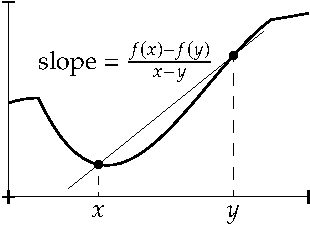
\includegraphics{figures/lipschitzfig}
\caption{The slope of a secant line.
A function is Lipschitz if %$\abs{\text{slope}} =
$\abs{\frac{f(x)-f(y)}{x-y}} \leq K$ for all $x$ and $y$.\label{fig:lipschitz}}
\end{myfigureht}

\begin{example}
The functions $\sin(x)$ and $\cos(x)$ are Lipschitz continuous.
In \exampleref{sincos:example} we have seen the following two inequalities.
\begin{equation*}
\abs{\sin(x)-\sin(y)} 
\leq \abs{x-y}
\qquad \text{and} \qquad
\abs{\cos(x)-\cos(y)}
\leq \abs{x-y} .
\end{equation*}

Hence sine and cosine are Lipschitz continuous with $K=1$.
\end{example}

\begin{example}
The function $f \colon [1,\infty) \to \R$ defined by $f(x) \coloneqq \sqrt{x}$
is Lipschitz continuous. Proof:
\begin{equation*}
\abs{\sqrt{x}-\sqrt{y}} = 
\abs{\frac{x-y}{\sqrt{x}+\sqrt{y}}}
=
\frac{\abs{x-y}}{\sqrt{x}+\sqrt{y}} .
\end{equation*}
As $x \geq 1$ and $y \geq 1$, we see that $\frac{1}{\sqrt{x}+\sqrt{y}}
\leq \frac{1}{2}$.  Therefore,
\begin{equation*}
\abs{\sqrt{x}-\sqrt{y}} = 
\abs{\frac{x-y}{\sqrt{x}+\sqrt{y}}}
\leq
\frac{1}{2}
\abs{x-y}.
\end{equation*}

On the other hand, $g \colon [0,\infty) \to \R$ defined by
$g(x) \coloneqq \sqrt{x}$ is not Lipschitz continuous.  Proof:
Suppose for all $x,y \in [0,\infty)$,
\begin{equation*}
\abs{\sqrt{x}-\sqrt{y}} 
\leq
K \abs{x-y} ,
\end{equation*}
for some $K$.  Set $y=0$ to obtain
$\sqrt{x} \leq K x$.   If $K > 0$, then for $x > 0$ we get
$\nicefrac{1}{K} \leq \sqrt{x}$ or $\nicefrac{1}{K^2} \leq x$.
This cannot possibly be true for all
$x > 0$.  Thus no such $K > 0$ exists and $g$ is not
Lipschitz continuous.  See \figureref{fig:sqrtgraph} and note how secant
lines would be more and more vertical as we get closer to $x=0$.
\begin{myfigureht}
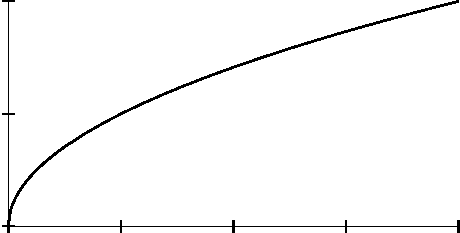
\includegraphics{figures/sqrtgraph}
\caption{Graph of $\sqrt{x}$ and some secant lines through $(0,0)$ and
$(x,\sqrt{x})$.\label{fig:sqrtgraph}}
\end{myfigureht}

The last example $g$ is a function that is uniformly
continuous but not Lipschitz continuous.
To see that $\sqrt{x}$ is
uniformly continuous as a function on $[0,\infty)$,
note that it is uniformly continuous when restricted to $[0,1]$ by \thmref{unifcont:thm}.
It is also Lipschitz (and so uniformly continuous) when restricted to $[1,\infty)$.
It is not hard (exercise) to show that this means that $\sqrt{x}$ is a
uniformly continuous function on $[0,\infty)$.
\end{example}

\subsection{Exercises}

\begin{exercise}
Let $f \colon S \to \R$ be uniformly continuous.  Let $A \subset S$.
Then the restriction $f|_A$ is uniformly continuous.
\end{exercise}

\begin{exercise}
Let $f \colon (a,b) \to \R$ be a uniformly continuous function.
Finish the proof of \propref{context:prop} by showing that
the limit
$\lim\limits_{x \to b} f(x)$
exists.
\end{exercise}

\begin{exercise}
Show that $f \colon (c,\infty) \to \R$ for some $c > 0$
and defined by $f(x) \coloneqq \nicefrac{1}{x}$ is Lipschitz continuous.
\end{exercise}

\begin{exercise}
Show that $f \colon (0,\infty) \to \R$
defined by $f(x) \coloneqq \nicefrac{1}{x}$ is not Lipschitz continuous.
\end{exercise}

\begin{samepage}
\begin{exercise}
Let $A, B$ be intervals.
Let $f \colon A \to \R$ and $g \colon B \to \R$ be uniformly continuous
functions such that $f(x) = g(x)$ for $x \in A \cap B$.  Define
the function $h \colon A \cup B \to \R$ by $h(x) \coloneqq f(x)$ if
$x \in A$ and $h(x) \coloneqq g(x)$ if $x \in B \setminus A$.
\begin{enumerate}[a)]
\item
Prove that if $A \cap B \not= \emptyset$, then $h$ is uniformly continuous.
\item
Find an example where $A \cap B = \emptyset$ and $h$ is not even
continuous.
\end{enumerate}
\end{exercise}
\end{samepage}

\begin{exercise}[Challenging]
Let $f \colon \R \to \R$ be a polynomial of degree 
$d \geq 2$.  Show that $f$ is not Lipschitz
continuous.
\end{exercise}

\begin{exercise}
Let $f \colon (0,1) \to \R$ be a bounded continuous function.  Show that
the function
$g(x) \coloneqq x(1-x)f(x)$ is uniformly continuous.
\end{exercise}

\begin{exercise}
Show that $f \colon (0,\infty) \to \R$ defined by $f(x) \coloneqq \sin
(\nicefrac{1}{x})$ is not uniformly continuous.
\end{exercise}

\begin{exercise}[Challenging]
Let $f \colon \Q \to \R$ be a uniformly continuous function.  Show that
there exists a uniformly continuous function $\widetilde{f} \colon \R \to \R$
such that $f(x) = \widetilde{f}(x)$ for all $x \in \Q$.
\end{exercise}

\begin{samepage}
\begin{exercise}
\leavevmode
\begin{enumerate}[a)]
\item
Find a continuous $f \colon (0,1) \to \R$ and a sequence
$\{ x_n \}_{n=1}^\infty$ in
$(0,1)$ that is Cauchy, but such that $\bigl\{ f(x_n) \bigr\}_{n=1}^\infty$ is not Cauchy.
\item
Prove that if $f \colon \R \to \R$ is continuous,
and $\{ x_n \}_{n=1}^\infty$ is
Cauchy, then $\bigl\{ f(x_n) \bigr\}_{n=1}^\infty$ is Cauchy.
\end{enumerate}
\end{exercise}
\end{samepage}

\begin{samepage}
\begin{exercise}
Prove:
\begin{enumerate}[a)]
\item
If $f \colon S \to \R$ and $g \colon S \to \R$ are uniformly continuous,
then $h \colon S \to \R$ given by $h(x) \coloneqq f(x) + g(x)$
is uniformly continuous.
\item
If $f \colon S \to \R$ is uniformly continuous and $a \in \R$,
then $h \colon S \to \R$ given by $h(x) \coloneqq a f(x)$
is uniformly continuous.
\end{enumerate}
\end{exercise}
\end{samepage}

\begin{exercise}
Prove:
\begin{enumerate}[a)]
\item
If $f \colon S \to \R$ and $g \colon S \to \R$ are Lipschitz,
then $h \colon S \to \R$ given by $h(x) \coloneqq f(x) + g(x)$
is Lipschitz.
\item
If $f \colon S \to \R$ is Lipschitz and $a \in \R$,
then $h \colon S \to \R$ given by $h(x) \coloneqq a f(x)$
is Lipschitz.
\end{enumerate}
\end{exercise}

\begin{exercise}
\pagebreak[2]
\leavevmode
\begin{enumerate}[a)]
\item
If $f \colon [0,1] \to \R$ is given by $f(x) \coloneqq x^m$ for an integer
$m \geq 0$,
show $f$ is Lipschitz and find the best (the smallest) Lipschitz constant
$K$ (depending on $m$ of course).
Hint: $(x-y)(x^{m-1} + x^{m-2}y + x^{m-3}y^2 + \cdots + x y^{m-2} + y^{m-1}) = x^m - y^m$.
\item
Using the previous exercise, show that if $f \colon [0,1] \to \R$
is a polynomial, that is, $f(x) \coloneqq a_m x^m + a_{m-1} x^{m-1} + \cdots + a_0$,
then $f$ is Lipschitz.
\end{enumerate}
\end{exercise}

\begin{exercise}
\pagebreak[2]
Suppose for $f \colon [0,1] \to \R$, we have $\abs{f(x)-f(y)} \leq K
\abs{x-y}$ for all $x,y$ in $[0,1]$,
and $f(0) = f(1) = 0$.
Prove that $\abs{f(x)} \leq \nicefrac{K}{2}$ for all $x \in [0,1]$.  Further show by example that
$\nicefrac{K}{2}$ is the best possible, that is, there exists such a continuous function
for which $\abs{f(x)} = \nicefrac{K}{2}$ for some $x \in [0,1]$.
\end{exercise}

\begin{exercise}
Suppose $f \colon \R \to \R$ is continuous and periodic with period
$P > 0$.  That is, $f(x+P) = f(x)$ for all $x \in \R$.  Show that $f$
is uniformly continuous.
\end{exercise}

\begin{exercise}
Suppose $f \colon S \to \R$ and $g \colon [0,\infty) \to [0,\infty)$
are functions, $g$ is continuous at $0$, $g(0) = 0$, and
whenever $x$ and $y$ are in $S$, we have $\abs{f(x)-f(y)} \leq
g\bigl(\abs{x-y}\bigr)$.
Prove that $f$ is uniformly continuous.
\end{exercise}

\begin{exercise}
Suppose $f \colon [a,b] \to \R$ is a function such that for every $c \in
[a,b]$ there is a $K_c > 0$ and an $\epsilon_c > 0$ for which
$\abs{f(x)-f(y)} \leq K_c \abs{x-y}$ for all $x$ and $y$ in
$(c-\epsilon_c,c+\epsilon_c) \cap [a,b]$.  In other words, $f$ is
\myquote{locally Lipschitz.}
\begin{enumerate}[a)]
\item
Prove that there exists a single $K > 0$ such that
$\abs{f(x)-f(y)} \leq K \abs{x-y}$ for all $x,y$ in $[a,b]$.
\item
Find a counterexample to the above if the interval is open, that is,
find an $f \colon (a,b) \to \R$ that is locally Lipschitz, but not
Lipschitz.
\end{enumerate}
\end{exercise}

%%%%%%%%%%%%%%%%%%%%%%%%%%%%%%%%%%%%%%%%%%%%%%%%%%%%%%%%%%%%%%%%%%%%%%%%%%%%%%

\sectionnewpage
\section{Limits at infinity}
\label{sec:limitatinf}

%mbxINTROSUBSECTION

\sectionnotes{less than 1 lecture (optional, can safely be omitted unless
\sectionref{sec:monotonefunc} or
\sectionref{sec:impropriemann} is also covered)}

\subsection{Limits at infinity}

As for sequences, a continuous variable can also approach infinity.

\begin{defn}
We say $\infty$ is a \emph{\myindex{cluster point}} of $S \subset \R$ if for every
$M \in \R$, there exists an $x \in S$ such that $x \geq M$.  Similarly,
$- \infty$ is a \emph{cluster point} of $S \subset \R$ if for every
$M \in \R$, there exists an $x \in S$ such that $x \leq M$.

\index{limit!of a function at infinity}%
Let $f \colon S \to \R$ be a function, where 
$\infty$ is a cluster point of $S$.
If there exists an $L \in \R$
such that for every $\epsilon > 0$, there is an $M \in \R$ such that
\begin{equation*}
\abs{f(x) - L} < \epsilon 
\end{equation*}
whenever $x \in S$ and $x \geq M$, then we say $f(x)$
\emph{converges}\index{converges!function} to $L$
as $x$ goes to $\infty$.  We call $L$ the \emph{limit}
and write
\glsadd{not:limfuncinf}
\begin{equation*}
\lim_{x \to \infty} f(x) \coloneqq L .
\end{equation*}
Alternatively we write $f(x) \to L$ as $x \to \infty$.

Similarly, if $-\infty$ is a cluster point of $S$
and
there exists an $L \in \R$
such that for every $\epsilon > 0$, there is an $M \in \R$ such that
\begin{equation*}
\abs{f(x) - L} < \epsilon 
\end{equation*}
whenever $x \in S$ and $x \leq M$, then we say $f(x)$ \emph{converges} to $L$
as $x$ goes to $-\infty$.
Alternatively, we write $f(x) \to L$ as $x \to -\infty$.
We call $L$ a \emph{limit} and, if unique, write
\begin{equation*}
\lim_{x \to -\infty} f(x) \coloneqq L .
\end{equation*}
\end{defn}

The first thing to do, as usual, is to prove that the limit, if it exists,
is unique.
We leave it as an exercise for the reader.

\begin{prop} \label{liminfty:unique}
The limit at $\infty$ or $-\infty$ as defined above is unique if it exists.
\end{prop}

\begin{example}
Let $f(x) \coloneqq \frac{1}{\abs{x}+1}$.  Then
\begin{equation*}
\lim_{x\to \infty} f(x) = 0 \qquad \text{and} \qquad
\lim_{x\to -\infty} f(x) = 0 .
\end{equation*}

Proof:
Let $\epsilon > 0$ be given.  Find $M > 0$ large enough
so that $\frac{1}{M+1} < \epsilon$.  If
$x \geq M$, then $0 < \frac{1}{\abs{x}+1} = \frac{1}{x+1} \leq \frac{1}{M+1} < \epsilon$.
The first limit follows.
The proof for $-\infty$ is left to the reader.
\end{example}

\begin{example}
Let $f(x) \coloneqq \sin(\pi x)$.  Then $\lim_{x\to\infty} f(x)$ does not exist.
To prove this fact note that if $x = 2n+\nicefrac{1}{2}$ for some $n \in
\N$, then $f(x)=1$,
while if $x = 2n+\nicefrac{3}{2}$, then $f(x)=-1$.  So they cannot both be
within a small $\epsilon$ of a single real number.

Be careful not to confuse continuous limits with limits of sequences.
We could say
\begin{equation*}
\lim_{n \to \infty} \sin(\pi n) = 0, \qquad \text{but} \qquad
\lim_{x \to \infty} \sin(\pi x) \enspace \text{does not exist}.
\end{equation*}
Of course the notation is ambiguous:  Are we thinking of the
sequence $\bigl\{ \sin (\pi n) \bigr\}_{n=1}^\infty$ or the function $\sin(\pi x)$
of a real variable?  We are simply using the convention
that $n \in \N$, while $x \in \R$.  When the notation is not clear,
it is good to explicitly mention where the variable lives, or what kind
of limit are you using.  If there is possibility of confusion, one can
write, for example,
\begin{equation*}
\lim_{\substack{n \to \infty\\n \in \N}} \sin(\pi n) .
\end{equation*}
\end{example}

There is a connection of continuous limits to limits of sequences, but we must take all
sequences going to infinity, just as before in \lemmaref{seqflimit:lemma}.

\begin{lemma} \label{seqflimitinf:lemma}
Suppose $f \colon S \to \R$ is a function, $\infty$ is a cluster
point of $S \subset \R$, and $L \in \R$.  Then
\begin{equation*}
\lim_{x\to\infty} f(x) = L
\qquad \text{if and only if} \qquad
\lim_{n\to\infty} f(x_n) = L
\end{equation*}
for all sequences $\{ x_n \}_{n=1}^\infty$ in $S$ such that $\lim\limits_{n\to\infty} x_n = \infty$.
\end{lemma}

The lemma also holds for the limit as $x \to -\infty$.
Its proof is almost identical and
is left as an exercise.

\begin{proof}
First suppose $f(x) \to L$ as $x \to \infty$.
Given an $\epsilon > 0$, there exists an $M$ such that for all $x \geq M$,
we have $\abs{f(x)-L} < \epsilon$.
Let $\{ x_n \}_{n=1}^\infty$
be a sequence in $S$ such that $\lim_{n\to\infty} x_n = \infty$.  Then there exists an
$N$ such that for all $n \geq N$, we have $x_n \geq M$.  And thus
$\abs{f(x_n)-L} < \epsilon$.

We prove the converse by contrapositive.  Suppose $f(x)$ does
not go to $L$ as $x \to \infty$.
This means that there exists an $\epsilon > 0$,
such that for every $n \in \N$, there exists an $x \in S$, $x \geq n$, let
us call it $x_n$, such that $\abs{f(x_n)-L} \geq \epsilon$.
Consider the sequence $\{ x_n \}_{n=1}^\infty$.  Clearly 
$\bigl\{ f(x_n) \bigr\}_{n=1}^\infty$ does not converge to $L$.  It remains to note
that $\lim_{n\to\infty} x_n = \infty$, because $x_n \geq n$ for all $n$.
\end{proof}

Using the lemma, we again translate results about sequential
limits into results about continuous limits as $x$ goes to infinity.  That
is, we have almost immediate analogues of the corollaries
in \sectionref{subseq:sequentiallimits}.  We simply allow 
the cluster point $c$ to be either $\infty$ or $-\infty$, in addition
to a real number.  We leave it to
the student to verify these statements.

\subsection{Infinite limit}

Just as for sequences, it is often convenient to distinguish certain
divergent sequences, and talk about limits being infinite
almost as if the limits existed.

\begin{defn}
\index{infinite limit!of a function}\index{limit!infinite}%
Let $f \colon S \to \R$ be a function and suppose 
$S$ has $\infty$ as a cluster point.
We say $f(x)$
\emph{\myindex{diverges to infinity}} 
as $x$ goes to $\infty$
if for every $N \in \R$
there exists an $M \in \R$ such that
\begin{equation*}
f(x) > N
\end{equation*}
whenever $x \in S$ and $x \geq M$.
We write
\begin{equation*}
\lim_{x \to \infty} f(x) \coloneqq \infty ,
\end{equation*}
or we say that $f(x) \to \infty$ as $x \to \infty$.
\end{defn}

A similar definition can be made for limits as $x \to -\infty$
or as $x \to c$ for a finite $c$.  Also similar definitions can be
made for limits being $-\infty$.  Stating these definitions is left
as an exercise.
Note that
sometimes \emph{\myindex{converges to infinity}} is used.
We can again use sequential limits, and an analogue of 
\lemmaref{seqflimit:lemma} is left as an exercise.

\begin{example}
Let us show that $\lim\limits_{x \to \infty} \frac{1+x^2}{1+x} = \infty$.

Proof: For $x \geq 1$, we have
\begin{equation*}
\frac{1+x^2}{1+x} \geq 
\frac{x^2}{x+x}  = 
\frac{x}{2} .
\end{equation*}
Given $N \in \R$, take $M = \max \{ 2N+1 , 1 \}$.
If $x \geq M$, then $x \geq 1$ and $\nicefrac{x}{2} > N$.
So
\begin{equation*}
\frac{1+x^2}{1+x} \geq 
\frac{x}{2} > N .
\end{equation*}
\end{example}

\subsection{Compositions}

Finally, just as for limits at finite numbers we can compose functions
easily.

\begin{prop} \label{prop:inflimcompositions}
Suppose $f \colon A \to B$, $g \colon B \to \R$, $A, B \subset \R$, 
$a \in \R \cup \{ -\infty, \infty\}$ is a cluster point of $A$,
and $b \in \R \cup \{ -\infty, \infty\}$ is a cluster point of $B$.
Suppose 
\begin{equation*}
\lim_{x \to a} f(x) = b\qquad \text{and} \qquad \lim_{y \to b} g(y) = c
\end{equation*}
for some $c \in \R \cup \{ -\infty, \infty \}$.
If $b \in B$, then suppose $g(b) = c$.
Then
\begin{equation*}
\lim_{x \to a} g\bigl(f(x)\bigr) = c .
\end{equation*}
\end{prop}

The proof is straightforward, and left as an exercise.  We already
know the proposition when $a, b, c \in \R$, see Exercises
\ref{exercise:contlimitcomposition} and
\ref{exercise:contlimitbadcomposition}.  Again the requirement that $g$ is
continuous at $b$, if $b \in B$, is necessary.

\begin{example}
Let $h(x) \coloneqq e^{-x^2+x}$.  Then
\begin{equation*}
\lim_{x\to \infty} h(x) = 0 .
\end{equation*}

Proof:
The claim follows once we know
\begin{equation*}
\lim_{x\to \infty} -x^2+x = -\infty
\end{equation*}
and
\begin{equation*}
\lim_{y\to -\infty} e^y = 0 ,
\end{equation*}
which is usually proved when the exponential function is defined.
\end{example}

\subsection{Exercises}

\begin{exercise}
Prove \propref{liminfty:unique}.
\end{exercise}

\begin{exercise}
Let $f \colon [1,\infty) \to \R$ be a function.  Define
$g \colon (0,1] \to \R$ via $g(x) \coloneqq f(\nicefrac{1}{x})$.
Using the definitions of limits directly,
show that $\lim_{x\to 0^+} g(x)$
exists if and only if $\lim_{x\to \infty} f(x)$ exists, in which
case they are equal.
\end{exercise}

\begin{exercise}
Prove \propref{prop:inflimcompositions}.
\end{exercise}

\begin{exercise}
Let us justify terminology.
Let $f \colon \R \to \R$ be a function such that
$\lim_{x \to \infty} f(x) = \infty$ (diverges to infinity).
Show that $f(x)$ diverges (i.e.\ does not converge) as $x \to \infty$.
\end{exercise}

\begin{exercise}
Come up with the definitions for limits of $f(x)$ going to $-\infty$ as $x \to
\infty$, $x \to -\infty$, and as $x \to c$ for a finite $c \in \R$.
Then state the definitions for limits of $f(x)$ going to $\infty$ 
as $x \to -\infty$, and as $x \to c$ for a finite $c \in \R$.
\end{exercise}

\begin{exercise}
Suppose $P(x) \coloneqq x^n + a_{n-1} x^{n-1} + \cdots + a_1 x + a_0$ is a \emph{\myindex{monic polynomial}}
of degree $n \geq 1$ (monic means that the coefficient of $x^n$ is 1).
\begin{enumerate}[a)]
\item
Show that if $n$ is even, then $\lim\limits_{x\to\infty} P(x) = 
\lim\limits_{x\to-\infty} P(x) = \infty$.
\item
Show that if $n$ is odd, then
$\lim\limits_{x\to\infty} P(x) = \infty$ and
$\lim\limits_{x\to-\infty} P(x) = -\infty$ (see previous exercise).
\end{enumerate}
\end{exercise}

\begin{exercise}
Let $\{ x_n \}_{n=1}^\infty$ be a sequence.  Consider $S \coloneqq \N \subset \R$, and
$f \colon S \to \R$ defined by $f(n) \coloneqq x_n$.  Show that
the two notions of limit,
\begin{equation*}
\lim_{n\to\infty} x_n \qquad \text{and} \qquad
\lim_{x\to\infty} f(x) 
\end{equation*}
are equivalent.  That is, show that if one exists so does
the other one, and in this case they are equal.
\end{exercise}

\begin{exercise}
Extend \lemmaref{seqflimitinf:lemma} as follows.
Suppose $S \subset \R$ has a cluster point $c \in \R$, $c = \infty$,
or $c = -\infty$.  Let $f \colon S \to \R$ be a function and suppose
$L = \infty$ or $L = -\infty$.  Show that
\begin{equation*}
%mbxlatex \begin{aligned}
%mbxlatex &
\lim_{x\to c} f(x) = L
%mbxlatex \\
%mbxlatex &
\qquad \text{if and only if}
%mbxlatex \\
%mbxSTARTIGNORE
\qquad
%mbxENDIGNORE
%mbxlatex &
\lim_{n\to\infty} f(x_n) = L \enspace \text{for all sequences }
\{ x_n \}_{n=1}^\infty \text{ such that } \lim_{n\to\infty} x_n = c .
%mbxlatex \end{aligned}
\end{equation*}
\end{exercise}

\begin{exercise}
Suppose $f \colon \R \to \R$ is a 2-periodic function, that is $f(x +2) =
f(x)$ for all $x$.  Define $g \colon \R \to \R$ by 
\begin{equation*}
g(x) \coloneqq f\left(\frac{\sqrt{x^2+1}-1}{x}\right)
\end{equation*}
\begin{enumerate}[a)]
\item
Find the function $\varphi \colon (-1,1) \to \R$ such that
$g\bigl(\varphi(t)\bigr) = f(t)$, that is $\varphi^{-1}(x) = 
\frac{\sqrt{x^2+1}-1}{x}$.
\item
Show that $f$ is continuous if and only if $g$ is continuous and
\begin{equation*}
\lim_{x \to \infty} g(x) = 
\lim_{x \to -\infty} g(x) = 
f(1) = f(-1) .
\end{equation*}
\end{enumerate}
\end{exercise}

%%%%%%%%%%%%%%%%%%%%%%%%%%%%%%%%%%%%%%%%%%%%%%%%%%%%%%%%%%%%%%%%%%%%%%%%%%%%%%

\sectionnewpage
\section{Monotone functions and continuity}
\label{sec:monotonefunc}

%mbxINTROSUBSECTION

\sectionnotes{1 lecture (optional, can safely be omitted unless
\sectionref{sec:ift} is also covered, requires \sectionref{sec:limitatinf})}

\begin{defn}
Let $S \subset \R$.
We say $f \colon S \to \R$ is \emph{\myindex{increasing}}
(resp.\  \emph{\myindex{strictly increasing}}) if $x,y \in S$ with
$x < y$ implies $f(x) \leq f(y)$ (resp.\ $f(x) < f(y)$).
We define
\emph{\myindex{decreasing}} and
\emph{\myindex{strictly decreasing}} in the same way by switching the
inequalities for $f$.

If a function is either increasing or decreasing, we say it is
\emph{monotone}\index{monotone function}.  If it is
strictly increasing or strictly decreasing, we say it is
\emph{strictly monotone}\index{strictly monotone function}.
\end{defn}

Sometimes \emph{\myindex{nondecreasing}}
(resp.\ \emph{\myindex{nonincreasing}}) is used
for increasing (resp.\ decreasing) function to emphasize it is not
strictly increasing (resp.\ strictly decreasing).

If $f$ is increasing, then $-f$ is decreasing and vice versa.  Therefore,
many results about monotone functions can just be proved for, say, increasing
functions, and the results follow easily for decreasing functions.

\subsection{Continuity of monotone functions}

One-sided limits for monotone functions are computed
by computing infima and suprema.

\begin{prop} \label{prop:monotlimits}
Let $S \subset \R$, $c \in \R$,
$f \colon S \to \R$ be increasing,
and
$g \colon S \to \R$ be decreasing.
If $c$ is a cluster point of $S \cap (-\infty,c)$, then
\begin{equation*}
\lim_{x \to c^-} f(x) = \sup \{ f(x) : x < c, x \in S \}
%mbxSTARTIGNORE
\qquad \text{and} \qquad
%mbxENDIGNORE
%mbxlatex \quad \text{and} \quad
\lim_{x \to c^-} g(x) = \inf \{ g(x) : x < c, x \in S \} .
\end{equation*}
If $c$ is a cluster point of $S \cap (c,\infty)$, then
\begin{equation*}
\lim_{x \to c^+} f(x) = \inf \{ f(x) : x > c, x \in S \}
%mbxSTARTIGNORE
\qquad \text{and} \qquad
%mbxENDIGNORE
%mbxlatex \quad \text{and} \quad
\lim_{x \to c^+} g(x) = \sup \{ g(x) : x > c, x \in S \} .
\end{equation*}
If $\infty$ is a cluster point of $S$, then
\begin{equation*}
\lim_{x \to \infty} f(x) = \sup \{ f(x) : x \in S \}
%mbxSTARTIGNORE
\qquad \text{and} \qquad
%mbxENDIGNORE
%mbxlatex \quad \text{and} \quad
\lim_{x \to \infty} g(x) = \inf \{ g(x) : x \in S \} .
\end{equation*}
If $-\infty$ is a cluster point of $S$, then
\begin{equation*}
\lim_{x \to -\infty} f(x) = \inf \{ f(x) : x \in S \}
%mbxSTARTIGNORE
\qquad \text{and} \qquad
%mbxENDIGNORE
%mbxlatex \quad \text{and} \quad
\lim_{x \to -\infty} g(x) = \sup \{ g(x) : x \in S \} .
\end{equation*}
\end{prop}

Namely, all the one-sided limits exist whenever they make
sense.  For monotone functions therefore, when we say
the left-hand limit $x \to c^-$
exists, we mean that $c$ is a cluster point of $S \cap (-\infty,c)$,
and same for the right-hand limit.

\begin{proof}
Let us assume $f$ is increasing, and we will show the first
equality.  The rest of the proof is very similar and is left as an
exercise.

Let $a \coloneqq \sup \{ f(x) : x < c, x \in S \}$.  If $a = \infty$,
then given an $M \in \R$, there exists an $x_M \in S$, $x_M < c$, such that $f(x_M) > M$. 
As $f$ is increasing, $f(x) \geq f(x_M) >  M$ for all $x \in S$ with $x > x_M$.
Take $\delta \coloneqq c-x_M > 0$ to obtain the definition of the limit going to
infinity.

Next suppose $a < \infty$.
Let $\epsilon > 0$ be given.  Because $a$ is the supremum and
$S \cap (-\infty,c)$ is nonempty, $a \in \R$ and
there exists an
$x_\epsilon \in S$,
$x_\epsilon < c$,
such that $f(x_\epsilon) > a-\epsilon$.  As $f$ is increasing,
if $x \in S$ and $x_\epsilon < x < c$, we have
$a-\epsilon < f(x_\epsilon) \leq f(x) \leq a$.  Let
$\delta \coloneqq c-x_\epsilon$.  Then for $x \in S \cap (-\infty,c)$
with $\abs{x-c} < \delta$,
we have $\abs{f(x)-a} < \epsilon$.
\end{proof}

Suppose $f \colon S \to \R$ is increasing, $c \in S$, and
that both one-sided limits exist.
Since $f(x) \leq f(c) \leq f(y)$
whenever $x < c < y$, taking the limits we obtain
\begin{equation*}
\lim_{x \to c^-} f(x) \leq f(c) \leq \lim_{x \to c^+} f(x) .
\end{equation*}
Then $f$ is continuous at $c$ if and only if both limits are equal
to each other (and hence equal to $f(c)$).  See also
\propref{prop:onesidedlimits}.
See \figureref{fig:figinccont} to get an idea of what a discontinuity
looks like.


\begin{cor} \label{cor:continterval}
If $I \subset \R$ is an interval and $f \colon I \to \R$ is 
monotone and not constant, then $f(I)$ is an interval if and only if $f$
is continuous.
\end{cor}

Assuming $f$ is not constant is to avoid the technicality
that $f(I)$ is a single point: $f(I)$ is a single
point if and only if $f$ is constant.  A constant function is 
continuous.

\begin{proof}
Without loss of generality, suppose $f$ is increasing.

First suppose $f$ is continuous.  Take two points
$f(x_1), f(x_2)$ in $f(I)$ and suppose
$f(x_1) < f(x_2)$.
As $f$ is increasing, then $x_1 < x_2$.  By the
\hyperref[IVT:thm]{intermediate value theorem},
given $y$ with $f(x_1) < y < f(x_2)$, we find
a $c \in (x_1,x_2) \subset I$ such that $f(c) = y$, so $y \in f(I)$. 
Hence, $f(I)$ is an interval.

Let us prove the reverse direction by contrapositive.
Suppose $f$ is not continuous at $c \in I$,
and that $c$ is not an endpoint of $I$.
Let
\begin{equation*}
%mbxlatex \begin{aligned}
a
%mbxlatex &
\coloneqq \lim_{x \to c^-} f(x) = \sup \bigl\{ f(x) : x \in I, x < c \bigr\} ,
%mbxSTARTIGNORE
\qquad
%mbxENDIGNORE
%mbxlatex \\
b
%mbxlatex &
\coloneqq \lim_{x \to c^+} f(x) = \inf \bigl\{ f(x) : x \in I, x > c \bigr\} .
%mbxlatex \end{aligned}
\end{equation*}
As $c$ is a discontinuity, $a < b$.
If $x < c$, then $f(x) \leq a$, and
if $x > c$, then $f(x) \geq b$.  Therefore
no point
in $(a,b) \setminus \bigl\{ f(c) \bigr\}$ is in $f(I)$.
There exists $x_1 \in I$ with $x_1 < c$, so
$f(x_1) \leq a$, and there exists $x_2 \in I$ with $x_2 > c$,
so $f(x_2) \geq b$.  Both $f(x_1)$ and $f(x_2)$ are in $f(I)$,
but there are points in between them that are not in $f(I)$.
So $f(I)$ is not an interval.  See \figureref{fig:figinccont}.

When $c \in I$ is an endpoint, the proof is similar and is left as an exercise.
\end{proof}

\begin{myfigureht}
\subimport*{figures/}{figinccont.pdf_t}
\caption{Increasing function $f \colon I \to \R$ discontinuity at
$c$.\label{fig:figinccont}}
\end{myfigureht}

A striking property of monotone functions is that they cannot have
too many discontinuities.

\begin{cor} \label{cor:monotcountcont}
Let $I \subset \R$ be an interval and
$f \colon I \to \R$ be monotone.  Then $f$ has at most
countably many discontinuities.
\end{cor}

\begin{proof}
Let $E \subset I$ be the set of all discontinuities
that are not endpoints of $I$.  As there are
only two endpoints, it is enough to show that $E$ is countable.
Without loss of generality, suppose $f$ is increasing.
We will define an injection $h \colon E \to \Q$.
For each $c \in E$,
both one-sided limits of $f$ exist as $c$ is not an endpoint.
Let
\begin{equation*}
%mbxlatex \begin{aligned}
a
%mbxlatex &
\coloneqq \lim_{x \to c^-} f(x) = \sup \bigl\{ f(x) : x \in I, x < c \bigr\} ,
%mbxSTARTIGNORE
\qquad
%mbxENDIGNORE
%mbxlatex \\
b
%mbxlatex &
\coloneqq \lim_{x \to c^+} f(x) = \inf \bigl\{ f(x) : x \in I, x > c \bigr\} .
%mbxlatex \end{aligned}
\end{equation*}
As $c$ is a discontinuity, $a < b$.  
There exists a rational number $q \in (a,b)$, so let $h(c) \coloneqq q$.
Suppose $d \in E$ is another discontinuity.
If $d > c$, there
exist an $x \in I$ with $c < x < d$, and so $\lim_{x \to d^-} f(x) \geq b$.
Hence the rational number we choose for $h(d)$ is different from $q$,
since $q=h(c) < b$ and $h(d) > b$.
Similarly if $d < c$.  After making such a choice for
every element of $E$, we have a 
one-to-one (injective) function into $\Q$.  Therefore, $E$ is countable.
\end{proof}

\begin{example} \label{example:countdiscont}
By $\lfloor x \rfloor$ denote the largest integer less than or equal to $x$.
Define $f \colon [0,1] \to \R$ by
\begin{equation*}
f(x) \coloneqq
x +
\sum_{n=0}^{\lfloor 1/(1-x) \rfloor}
2^{-n} ,
\end{equation*}
for $x < 1$ and $f(1) \coloneqq 3$.
It is an exercise to show that $f$ is strictly increasing, bounded, and
has a discontinuity at all points $1-\nicefrac{1}{k}$ for $k \in \N$.  In particular,
there are countably many discontinuities, but the function is bounded and
defined on a closed bounded interval.  See \figureref{fig:countdiscont}.
\begin{myfigureht}
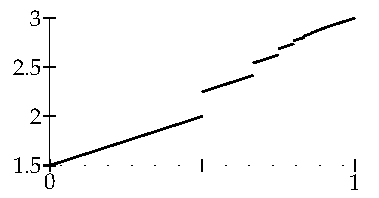
\includegraphics{figures/increasing-discont-fig}
\caption{Strictly increasing function on $[0,1]$ with countably many
discontinuities.\label{fig:countdiscont}}
\end{myfigureht}

Similarly, one can find an example of a monotone function discontinuous on a dense set
such as the rational numbers.  See the exercises.
\end{example}


\subsection{Continuity of inverse functions}


A strictly monotone function $f$ is one-to-one (injective).
To see this fact,
notice that if $x \not= y$, then we can assume $x < y$.  Either $f(x) <
f(y)$ if $f$ is strictly increasing or $f(x) > f(y)$ if $f$ is strictly
decreasing, so $f(x) \not= f(y)$.
Hence, $f$ must have an inverse $f^{-1}$ defined on its range.

\begin{prop} \label{prop:invcont}
If $I \subset \R$ is an interval and $f \colon I \to \R$ is strictly
monotone, then the inverse $f^{-1} \colon f(I) \to I$ is continuous.
\end{prop}

\begin{proof}
Suppose $f$ is strictly increasing.  The proof is almost
identical for a strictly decreasing function.
Since $f$ is strictly increasing, so is $f^{-1}$.  That is, if $f(x) <
f(y)$, then we must have $x < y$ and therefore
$f^{-1}\bigl(f(x)\bigr) < f^{-1}\bigl(f(y)\bigr)$.

Take $c \in f(I)$.
If $c$ is not a cluster point of $f(I)$, then $f^{-1}$ is continuous at $c$
automatically.  So let $c$ be a cluster point of $f(I)$.
Suppose both of the following one-sided limits exist:
\begin{align*}
x_0 & \coloneqq \lim_{y \to c^-} f^{-1}(y) =
\sup \bigl\{ f^{-1}(y) : y < c, y \in f(I) \bigr\}
=
\sup \bigl\{ x \in I : f(x) < c \bigr\} , \\
x_1 & \coloneqq \lim_{y \to c^+} f^{-1}(y) =
\inf \bigl\{ f^{-1}(y) : y > c, y \in f(I) \bigr\}
=
\inf \bigl\{ x \in I : f(x) > c \bigr\} .
\end{align*}
We have $x_0 \leq x_1$ as $f^{-1}$ is increasing.
For all $x \in I$ where $x > x_0$, we have $f(x) \geq c$.  As $f$ is strictly increasing,
we must have $f(x) > c$ for all $x \in I$ where $x > x_0$.  Therefore,
\begin{equation*}
\{ x \in I : x > x_0 \} \subset \bigl\{ x \in I : f(x) > c \bigr\}.
\end{equation*}
The infimum of the left-hand set is $x_0$, and the infimum of the right-hand
set is $x_1$, so we obtain $x_0 \geq x_1$.
So $x_1 = x_0$, and $f^{-1}$ is continuous at $c$.

If one of the one-sided limits does not exist, the argument is similar
and is left as an exercise.
\end{proof}

\begin{example}
The proposition does not require $f$ itself to be continuous.  Let
$f \colon \R \to \R$ be defined by
\begin{equation*}
f(x) \coloneqq
\begin{cases}
x & \text{if } x < 0, \\
x+1 & \text{if } x \geq 0. \\
\end{cases}
\end{equation*}
The function $f$ is not continuous at $0$.
The image of $I = \R$ is the set 
$(-\infty,0)\cup [1,\infty)$, not an interval.
Then $f^{-1} \colon (-\infty,0)\cup [1,\infty)
\to \R$ can be written as
\begin{equation*}
f^{-1}(y) =
\begin{cases}
y & \text{if } y < 0, \\
y-1 & \text{if } y \geq 1. 
\end{cases}
\end{equation*}
It is not difficult to see that $f^{-1}$ is a continuous function.  See
\figureref{invcontfig} for the graphs.
\begin{myfigureht}
\subimport*{figures/}{invcontfigAB.pdf_t}
\caption{Graph of $f$ on the left and $f^{-1}$ on the right.\label{invcontfig}}
\end{myfigureht}
\end{example}

Notice what happens with the proposition if $f(I)$ is an interval.
In that case, we could simply
apply \corref{cor:continterval} to both $f$ and $f^{-1}$.  That is, if
$f \colon I \to J$ is an onto strictly monotone function and $I$ and $J$ are intervals,
then both $f$ and $f^{-1}$ are continuous.  Furthermore, $f(I)$ is an
interval precisely when $f$ is continuous.

\subsection{Exercises}

\begin{exercise}
Suppose $f \colon [0,1] \to \R$ is monotone.  Prove $f$ is bounded.
\end{exercise}

\begin{exercise}
Finish the proof of \propref{prop:monotlimits}.
Hint: You can halve your work by noticing that if $g$ is decreasing,
then $-g$ is increasing.
\end{exercise}

\begin{exercise}
Finish the proof of \corref{cor:continterval}.
\end{exercise}

\begin{exercise}
Prove the claims in \exampleref{example:countdiscont}.
\end{exercise}

\begin{exercise}
Finish the proof of \propref{prop:invcont}.
\end{exercise}

\begin{samepage}
\begin{exercise}
Suppose $S \subset \R$, and $f \colon S \to \R$ is an increasing
function.  Prove:
\begin{enumerate}[a)]
\item
If $c$ is a cluster point
of $S \cap (c,\infty)$, then
$\lim\limits_{x\to c^+} f(x) < \infty$.
\item
If $c$ is a cluster point of $S \cap (-\infty,c)$
and $\lim\limits_{x\to c^-} f(x) = \infty$, then
$S \subset (-\infty,c)$.
\end{enumerate}
\end{exercise}
\end{samepage}

\begin{exercise}
Let $I \subset \R$ be an interval and $f \colon I \to \R$ a function.
Suppose that for each $c \in I$, there exist $a, b \in \R$ with
$a > 0$ such that $f(x) \geq a x + b$ for all $x \in I$
and $f(c) = a c + b$.  Show that $f$ is strictly increasing.
\end{exercise}

\begin{exercise}
Suppose $I$ and $J$ are intervals and
$f \colon I \to J$ is a continuous, bijective (one-to-one and onto)
function.  Show that $f$ is strictly monotone.
\end{exercise}

\begin{exercise}
Consider a monotone function $f \colon I \to \R$ on an interval $I$.  Prove that there exists
a function $g \colon I \to \R$ such that
$\lim\limits_{x \to c^-} g(x) = g(c)$ for all $c$ in $I$ except the
smaller (left) endpoint of $I$, and such that
$g(x) = f(x)$ for all but countably many $x \in I$.
\end{exercise}

\begin{exercise}
\leavevmode
\begin{enumerate}[a)]
\item
Let $S \subset \R$ be a subset.  If $f \colon S \to \R$ is increasing and
bounded,
then show that there exists an increasing $F \colon \R \to \R$
such that $f(x) = F(x)$ for all $x \in S$.
\item
Find an example of a strictly increasing bounded $f \colon S \to \R$ such that
an increasing $F$ as above is never strictly increasing.
\end{enumerate}
\end{exercise}

\begin{exercise}[Challenging] \label{exercise:increasingfuncdiscatQ}
Find an example of an increasing function $f \colon [0,1] \to \R$
that has a discontinuity at each rational number.  Then show that the image
$f\bigl([0,1]\bigr)$ contains no interval.  Hint: Enumerate
the rational numbers and define
the function with a series.
\end{exercise}

\begin{exercise}
Suppose $I$ is an interval and $f \colon I \to \R$ is monotone.
Show that $\R \setminus f(I)$ is a countable union of disjoint intervals.
\end{exercise}

\begin{exercise}
Suppose $f \colon [0,1] \to (0,1)$ is increasing.  Show that for every
$\epsilon > 0$, there exists
a strictly increasing $g \colon [0,1] \to (0,1)$ such that
$g(0) = f(0)$, $f(x) \leq g(x)$ for all $x$, and $g(1)-f(1) < \epsilon$.
\end{exercise}

\begin{exercise}
Prove that the \myindex{Dirichlet function}
$f \colon [0,1] \to\R$, defined by $f(x) \coloneqq 1$
if $x$ is rational and $f(x) \coloneqq 0$ otherwise, cannot be written as a
difference of two increasing functions.  That is, there do not exist
increasing $g$ and $h$ such that, $f(x) = g(x) - h(x)$.
\end{exercise}

\begin{exercise}
Suppose $f \colon (a,b) \to (c,d)$ is a strictly increasing
onto function.  Prove that there exists a $g \colon (a,b) \to (c,d)$,
which is also strictly increasing and onto, and $g(x) < f(x)$ for all $x \in
(a,b)$.
\end{exercise}




%%%%%%%%%%%%%%%%%%%%%%%%%%%%%%%%%%%%%%%%%%%%%%%%%%%%%%%%%%%%%%%%%%%%%%%%%%%%%%

% The Derivative chapter
\chapter{The Derivative} \label{der:chapter}

%%%%%%%%%%%%%%%%%%%%%%%%%%%%%%%%%%%%%%%%%%%%%%%%%%%%%%%%%%%%%%%%%%%%%%%%%%%%%%

\section{The derivative}
\label{sec:der}

\sectionnotes{1 lecture}

The idea of a derivative is the following.
If the graph of a function looks locally like a straight line,
then we can then talk about the slope of this line.
The slope tells us the rate at which 
the value of the function is changing at that particular point.
Of course, we are leaving out any function that has corners or
discontinuities.  
Let us be precise.

\subsection{Definition and basic properties}

\begin{defn}
Let $I$ be an interval, let
$f \colon I \to \R$ be a function, and let $c \in I$.  If 
the limit
\begin{equation*}
L := \lim_{x \to c} \frac{f(x)-f(c)}{x-c} 
\end{equation*}
exists, then we say $f$ is
\emph{\myindex{differentiable}}\index{function!differentiable} at
$c$, that $L$ is the \emph{\myindex{derivative}} of $f$ at $c$,
and write $f'(c) := L$.\glsadd{not:derivative}

\medskip

If $f$ is differentiable at all $c \in I$, then we simply say that
$f$ is \emph{differentiable}, and then we obtain a function
$f' \colon I \to \R$.
The derivative is sometimes written as $\frac{df}{dx}$ or
$\frac{d}{dx}\bigl( f(x) \bigr)$.

\medskip

The expression $\frac{f(x)-f(c)}{x-c}$ is called the
\emph{\myindex{difference quotient}}.
\end{defn}

The graphical interpretation of the derivative is  depicted in
\figureref{derivfig}.  The left-hand plot gives the line through
$\bigl(c,f(c)\bigr)$
and $\bigl(x,f(x)\bigr)$ with slope
$\frac{f(x)-f(c)}{x-c}$, that is,
the so-called \emph{\myindex{secant line}}.  When we take the limit as $x$ goes to $c$,
we get the right-hand plot, where we see
that the derivative of the function
at the point $c$ is the slope of the line tangent to the graph of $f$
at the point $\bigl(c,f(c)\bigr)$.

\begin{myfigureht}
\subimport*{figures/}{deriv_derivd.pdf_t}
\caption{Graphical interpretation of the derivative.\label{derivfig}}
\end{myfigureht}

We allow $I$ to be a closed interval and we allow
$c$ to be an endpoint of $I$.  Some calculus books do not allow $c$ to be an
endpoint of an interval, but all the theory still works by allowing it, and
it makes our work easier.

\begin{example}
Let $f(x) := x^2$ defined on the whole real line.  Let $c \in \R$ be arbitrary.  We find that if
$x \not=c$,
\begin{equation*}
\frac{x^2-c^2}{x-c} =
\frac{(x+c)(x-c)}{x-c} =
(x+c) .
\end{equation*}
Therefore,
\begin{equation*}
f'(c) = 
\lim_{x\to c} \frac{x^2-c^2}{x-c} =
\lim_{x\to c} (x+c) = 2c.
\end{equation*}
\end{example}

\begin{example}
Let $f(x) := ax + b$ for numbers $a, b \in \R$.
Let $c \in \R$ be arbitrary.
For $x \not=c$,
\begin{equation*}
\frac{f(x)-f(c)}{x-c} =
\frac{a(x-c)}{x-c} = a .
\end{equation*}
Therefore,
\begin{equation*}
f'(c) =
\lim_{x\to c} 
\frac{f(x)-f(c)}{x-c} =
\lim_{x\to c} 
a = a.
\end{equation*}
In fact, every differentiable function \myquote{infinitesimally} behaves like
the affine function $ax + b$.  You can guess many results
and formulas for derivatives, if you work them out for affine functions
first.
\end{example}

\begin{example}
The function $f(x) := \sqrt{x}$ is differentiable for $x > 0$.  To see this
fact, fix $c > 0$,
and take $x \not= c$, $x > 0$.  Compute
\begin{equation*}
\frac{\sqrt{x}-\sqrt{c}}{x-c}
=
\frac{\sqrt{x}-\sqrt{c}}{(\sqrt{x}-\sqrt{c})(\sqrt{x}+\sqrt{c})}
=
\frac{1}{\sqrt{x}+\sqrt{c}} .
\end{equation*}
Therefore,
\begin{equation*}
f'(c) =
\lim_{x\to c}
\frac{\sqrt{x}-\sqrt{c}}{x-c}
=
\lim_{x\to c}
\frac{1}{\sqrt{x}+\sqrt{c}}
=
\frac{1}{2\sqrt{c}} .
\end{equation*}
\end{example}

\begin{example}
The function $f(x) := \abs{x}$ is not differentiable
at the origin.  When $x > 0$,
\begin{equation*}
\frac{\abs{x}-\abs{0}}{x-0} =
\frac{x-0}{x-0} = 1 .
\end{equation*}
When $x < 0$,
\begin{equation*}
\frac{\abs{x}-\abs{0}}{x-0} =
\frac{-x-0}{x-0} = -1 .
\end{equation*}
\end{example}

A famous example of Weierstrass shows that there exists a continuous
function that is not differentiable at \emph{any} point.  The construction
of this function is beyond the scope of this chapter.  On the other hand,
a differentiable function is always continuous.

\begin{prop}
Let $f \colon I \to \R$ be differentiable at $c \in I$,
then it is continuous at $c$.
\end{prop}

\begin{proof}
We know the limits
\begin{equation*}
\lim_{x\to c}\frac{f(x)-f(c)}{x-c} = f'(c)
\qquad
\text{and}
\qquad
\lim_{x\to c}(x-c) = 0
\end{equation*}
exist.  Furthermore,
\begin{equation*}
f(x)-f(c) = 
\left( \frac{f(x)-f(c)}{x-c} \right) (x-c) .
\end{equation*}
Therefore, the limit of $f(x)-f(c)$ exists and
\begin{equation*}
\lim_{x\to c} \bigl( f(x)-f(c) \bigr) =
\left(\lim_{x\to c} \frac{f(x)-f(c)}{x-c} \right)
\left(\lim_{x\to c} (x-c) \right) =
f'(c) \cdot 0  = 0.
\end{equation*}
Hence $\lim\limits_{x\to c} f(x) = f(c)$, and $f$ is continuous at $c$.
\end{proof}

An important property of the derivative is linearity.  The
derivative is the approximation of a function by a straight line.
The slope of a line through two points changes linearly when the
$y$-coordinates are changed linearly.  By taking the limit,
it makes sense that the derivative is linear.

\begin{prop}
\index{linearity of the derivative}
Let $I$ be an interval, let
$f \colon I \to \R$ and $g \colon I \to \R$ be differentiable at $c \in I$,
and let $\alpha \in \R$.
\begin{enumerate}[(i)]
\item
Define $h \colon I \to \R$ by $h(x) := \alpha f(x)$.  Then
$h$ is differentiable at $c$ and
$h'(c) = \alpha f'(c)$.
\item
Define $h \colon I \to \R$ by $h(x) :=  f(x) + g(x)$.  Then
$h$ is differentiable at $c$ and
$h'(c) =  f'(c) + g'(c)$.
\end{enumerate}
\end{prop}

\begin{proof}
First, let $h(x) := \alpha f(x)$.
For $x \in I$, $x \not= c$,
\begin{equation*}
\frac{h(x)-h(c)}{x-c} =
\frac{\alpha f(x) - \alpha f(c)}{x-c}
=
\alpha \frac{f(x) - f(c)}{x-c} .
\end{equation*}
The limit as $x$ goes to $c$ exists on the right-hand side
by \corref{falg:cor}.  We get
\begin{equation*}
\lim_{x\to c}\frac{h(x)-h(c)}{x-c} =
\alpha \lim_{x\to c} \frac{f(x) - f(c)}{x-c} .
\end{equation*}
Therefore, $h$ is differentiable at $c$,
and the derivative is computed as given.

Next, define $h(x) := f(x)+g(x)$.
For $x \in I$, $x \not= c$, we have
\begin{equation*}
\frac{h(x)-h(c)}{x-c} =
\frac{\bigl(f(x) + g(x)\bigr) - \bigl(f(c) + g(c)\bigr)}{x-c}
=
\frac{f(x) - f(c)}{x-c}
+
\frac{g(x) - g(c)}{x-c} .
\end{equation*}
The limit as $x$ goes to $c$ exists on the right-hand side
by \corref{falg:cor}.  We get
\begin{equation*}
\lim_{x\to c}\frac{h(x)-h(c)}{x-c} =
\lim_{x\to c} \frac{f(x) - f(c)}{x-c}
+
\lim_{x\to c}\frac{g(x) - g(c)}{x-c} .
\end{equation*}
Therefore, $h$ is differentiable at $c$,
and the derivative is computed as given.
\end{proof}

It is not true that the derivative of a multiple of two functions is
the multiple of the derivatives.  Instead we get the so-called \emph{product
rule} or the \emph{\myindex{Leibniz rule}}%
\footnote{Named for the German mathematician
\href{https://en.wikipedia.org/wiki/Leibniz}{Gottfried Wilhelm Leibniz}
(1646--1716).}.

\begin{prop}[Product rule]\index{product rule}
Let $I$ be an interval, let
$f \colon I \to \R$ and $g \colon I \to \R$ be 
functions differentiable at $c$.  If $h \colon I \to \R$
is defined by
\begin{equation*}
h(x) := f(x) g(x) ,
\end{equation*}
then $h$ is differentiable at $c$ and
\begin{equation*}
h'(c) = f(c) g'(c) + f'(c) g(c) .
\end{equation*}
\end{prop}

The proof of the product rule is left as an exercise.  The key to the proof is 
the identity
$f(x) g(x) - f(c) g(c) =
f(x)\bigl( g(x) - g(c) \bigr)
+ \bigl( f(x) - f(c) \bigr) g(c)$,
which is illustrated in \figureref{figprodrule}.
\begin{myfigureht}
\subimport*{figures/}{figprodrule.pdf_t}
\caption{The idea of product rule.  The area of the entire rectangle
$f(x)g(x)$ differs from the area of the white rectangle $f(c)g(c)$
by the area of the lightly shaded rectangle
$f(x)\bigl( g(x) - g(c) \bigr)$ plus the darker rectangle
$\bigl( f(x) - f(c) \bigr) g(c)$.
In other words, $\Delta (f \cdot g)
= f \cdot \Delta g + \Delta f \cdot g$.\label{figprodrule}}
\end{myfigureht}



\begin{prop}[Quotient Rule]\index{quotient rule}
Let $I$ be an interval, let
$f \colon I \to \R$ and $g \colon I \to \R$ be differentiable at $c$
and $g(x) \not= 0$ for all $x \in I$.
If $h \colon I \to \R$
is defined by
\begin{equation*}
h(x) := \frac{f(x)}{g(x)},
\end{equation*}
then $h$ is differentiable at $c$ and
\begin{equation*}
h'(c) = \frac{f'(c) g(c) - f(c) g'(c)}{{\bigl(g(c)\bigr)}^2} .
\end{equation*}
\end{prop}

Again, the proof is left as an exercise.

\subsection{Chain rule}

More complicated functions are often obtained by composition,
which is differentiated via the chain rule.  The rule also tells us
how a derivative changes if we change variables.

\begin{prop}[Chain Rule]
\index{chain rule}
Let $I_1, I_2$ be intervals, let
$g \colon I_1 \to I_2$ be differentiable at $c \in I_1$,
and
$f \colon I_2 \to \R$ be differentiable at $g(c)$.
If $h \colon I_1 \to \R$
is defined by
\begin{equation*}
h(x) := (f \circ g) (x) = f\bigl(g(x)\bigr) ,
\end{equation*}
then $h$ is differentiable at $c$ and
\begin{equation*}
h'(c) = f'\bigl(g(c)\bigr)g'(c) .
\end{equation*}
\end{prop}

\begin{proof}
Let $d := g(c)$.  Define
$u \colon I_2 \to \R$ and $v \colon I_1 \to \R$ by
\begin{equation*}
u(y) :=
\begin{cases}
 \frac{f(y) - f(d)}{y-d}  & \text{if } y \not=d, \\
 f'(d)                    & \text{if } y = d,
\end{cases}
\qquad
v(x) :=
\begin{cases}
 \frac{g(x) - g(c)}{x-c} & \text{if } x \not=c, \\
 g'(c)                   & \text{if } x = c.
\end{cases}
\end{equation*}
Because $f$ is differentiable at $d = g(c)$, we find that
$u$ is continuous at $d$.  Similarly, $v$ is continuous at $c$.
For any $x$ and $y$,
\begin{equation*}
f(y)-f(d) = u(y) (y-d)
\qquad \text{and} \qquad
g(x)-g(c) = v(x) (x-c) .
\end{equation*}
Plug in to obtain
\begin{equation*}
h(x)-h(c)
=
f\bigl(g(x)\bigr)-f\bigl(g(c)\bigr)
=
u\bigl( g(x) \bigr) \bigl(g(x)-g(c)\bigr)
=
u\bigl( g(x) \bigr) \bigl(v(x) (x-c)\bigr) .
\end{equation*}
Therefore, if $x \not= c$,
\begin{equation} \label{eq:chainruleeq}
\frac{h(x)-h(c)}{x-c}
=
u\bigl( g(x) \bigr) v(x) .
\end{equation}
By continuity of $u$ and $v$ at $d$ and $c$ respectively, we find
$\lim_{y \to d} u(y)
= f'(d) = f'\bigl(g(c)\bigr)$ and
$\lim_{x \to c} v(x) = g'(c)$.
The function $g$ is continuous at $c$, and so $\lim_{x \to c} g(x) = g(c)$.
Hence the limit of
the right-hand side of \eqref{eq:chainruleeq}
as $x$ goes to $c$
exists and is equal to $f'\bigl(g(c)\bigr) g'(c)$.  Thus $h$
is differentiable at $c$ and the limit is $f'\bigl(g(c)\bigr)g'(c)$.
\end{proof}

\subsection{Exercises}

\begin{exercise}
Prove the product rule.
Hint: Prove and use
$f(x) g(x) - f(c) g(c) = f(x)\bigl( g(x) - g(c) \bigr) + \bigl( f(x) -
f(c) \bigr) g(c)$.
\end{exercise}

\begin{exercise}
Prove the quotient rule.  Hint: You can do this directly, but it may be
easier to find the derivative of $\nicefrac{1}{x}$ and then use
the chain rule and the product rule.
\end{exercise}

\begin{exercise} \label{exercise:diffofxn}
For $n \in \Z$,
prove that $x^n$ is differentiable and find the derivative,
unless, of course, $n < 0$ and $x=0$.
Hint: Use the product rule.
\end{exercise}

\begin{exercise}
Prove that a polynomial is differentiable and find the derivative.
Hint: Use the previous exercise.
\end{exercise}

\begin{exercise}
Define $f \colon \R \to \R$ by
\begin{equation*}
f(x) :=
\begin{cases}
x^2 & \text{if } x \in \Q,\\
0 & \text{otherwise.}
\end{cases}
\end{equation*}
Prove that $f$ is differentiable at $0$, but discontinuous at all points
except $0$.
\end{exercise}

\begin{exercise}
Assume the inequality $\abs{x-\sin(x)} \leq x^2$.  Prove that $\sin$ is
differentiable at $0$, and find the derivative at $0$.
\end{exercise}

\begin{exercise}
Using the previous exercise, prove that $\sin$ is differentiable at all $x$
and that the derivative is $\cos(x)$.  Hint: Use the sum-to-product
trigonometric identity as we did before.
\end{exercise}

\begin{exercise}
Let $f \colon I \to \R$ be differentiable.  For $n \in \Z$, let $f^n$
be the function defined by $f^n(x) := {\bigl( f(x) \bigr)}^n$.  If
$n < 0$, assume $f(x) \not= 0$ for all $x \in I$.  Prove that
$(f^n)'(x) = n {\bigl(f(x) \bigr)}^{n-1} f'(x)$.
\end{exercise}

\begin{exercise}
Suppose $f \colon \R \to \R$ is a differentiable
Lipschitz continuous function.
Prove that $f'$ is a bounded function.
\end{exercise}

\begin{exercise}
Let $I_1, I_2$ be intervals.
Let $f \colon I_1 \to I_2$ be a bijective function and $g \colon I_2 \to I_1$
be the inverse.  Suppose that both $f$ is differentiable at $c \in I_1$ and
$f'(c) \not=0$ and $g$ is differentiable at $f(c)$.  Use the chain rule
to find a formula for $g'\bigl(f(c)\bigr)$ (in terms of $f'(c)$).
\end{exercise}

\begin{exercise} \label{exercise:bndmuldiff}
Suppose $f \colon I \to \R$ is bounded, $g \colon I \to
\R$ is differentiable at $c \in I$, and $g(c) = g'(c) = 0$.  Show
that $h(x) := f(x) g(x)$ is differentiable at $c$.  Hint: You
cannot apply the product rule.
\end{exercise}

\begin{exercise} \label{exercise:diffsqueeze}
Suppose $f \colon I \to \R$, 
$g \colon I \to \R$, and
$h \colon I \to \R$, are functions.  Suppose $c \in I$ is such that
$f(c) = g(c) = h(c)$, $g$ and $h$ are differentiable at $c$,
and $g'(c) = h'(c)$.  Furthermore suppose $h(x) \leq f(x) \leq g(x)$ for
all $x \in I$.  Prove $f$ is differentiable at $c$ and $f'(c) = g'(c) =
h'(c)$.
\end{exercise}

\begin{exercise}
Suppose $f \colon (-1,1) \to \R$ is a function such that $f(x) = x h(x)$ for a bounded
function $h$.
\begin{enumerate}[a)]
\item
Show that $g(x) := {\bigl( f(x) \bigr)}^2$ is
differentiable at the origin and $g'(0) = 0$.
\item
Find an example of a
continuous function $f \colon (-1,1) \to \R$ with $f(0) = 0$, but such
that $g(x) := {\bigl( f(x) \bigr)}^2$ is not differentiable at the origin.
\end{enumerate}
\end{exercise}

\begin{exercise}
Suppose $f \colon I \to \R$ is differentiable at $c \in I$.
Prove there exist numbers $a$ and $b$ with the property that
for every $\epsilon > 0$, there is a $\delta > 0$, such that
$\abs{a+b(x-c) - f(x)} \leq \epsilon \abs{x-c}$, whenever $x \in I$ and
$\abs{x-c} < \delta$.
In other words, show that
there exists a function $g \colon I \to \R$
such that $\lim_{x\to c} g(x) = 0$ and
$\abs{a+b(x-c) - f(x)} \leq \abs{x-c} g(x)$.
\end{exercise}

\begin{exercise} \label{exercise:simpleLHopital}
Prove the following simple version of \myindex{L'H\^opital's rule}\index{L'Hospital's rule}.
Suppose 
$f \colon (a,b) \to \R$ and $g \colon (a,b) \to \R$ are differentiable
functions
whose derivatives $f'$ and $g'$ are continuous functions.
Suppose that at $c \in (a,b)$, $f(c) = 0$, $g(c)=0$,
and
$g'(x) \not= 0$ for all $x \in (a,b)$, and suppose
that the limit of $\nicefrac{f'(x)}{g'(x)}$ as $x$ goes to $c$ exists.  Show that
\begin{equation*}
\lim_{x \to c} \frac{f(x)}{g(x)} = 
\lim_{x \to c} \frac{f'(x)}{g'(x)} .
\end{equation*}
\end{exercise}

%%%%%%%%%%%%%%%%%%%%%%%%%%%%%%%%%%%%%%%%%%%%%%%%%%%%%%%%%%%%%%%%%%%%%%%%%%%%%%

\sectionnewpage
\section{Mean value theorem}
\label{sec:mvt}

\sectionnotes{2 lectures (some applications may be skipped)}

\subsection{Relative minima and maxima}

We talked about absolute maxima and minima.  These are the tallest peaks and
lowest valleys in the whole mountain range.  What
about peaks of individual mountains and bottoms of individual valleys?
The derivative, being a local concept, is like walking around in a fog; it can't
tell you if you're on the highest peak, but it can help you find all the
individual peaks.

\begin{defn}
Let $S \subset \R$ be a set and
let $f \colon S \to \R$ be a function.  The function $f$ is said to have
a \emph{\myindex{relative maximum}}\index{maximum!relative}
at $c \in S$ if there exists a $\delta>0$
such that for all $x \in S$ where $\abs{x-c} < \delta$,
we have $f(x) \leq f(c)$.
The definition of
\emph{\myindex{relative minimum}}\index{minimum!relative}
is analogous.
\end{defn}

\begin{lemma}\label{relminmax:lemma}
Suppose $f \colon [a,b] \to \R$ is differentiable at $c \in (a,b)$,
and $f$ has
a relative minimum or a relative maximum at $c$.  Then
$f'(c) = 0$.
\end{lemma}

\begin{proof}
We prove the statement for a maximum.  For a minimum the statement
follows by considering the function $-f$.

Let $c$ be a relative maximum of $f$.  That is, there is a $\delta > 0$ such
that as long
as $\abs{x-c} < \delta$, we have $f(x)-f(c) \leq 0$.
We look at the difference
quotient.  If $c < x < c+\delta$, then
\begin{equation*}
\frac{f(x)-f(c)}{x-c} \leq 0 ,
\end{equation*}
and if $c-\delta < y < c$, then
\begin{equation*}
\frac{f(y)-f(c)}{y-c} \geq 0 .
\end{equation*}
See \figureref{fig:critpt} for an illustration.
\begin{myfigureht}
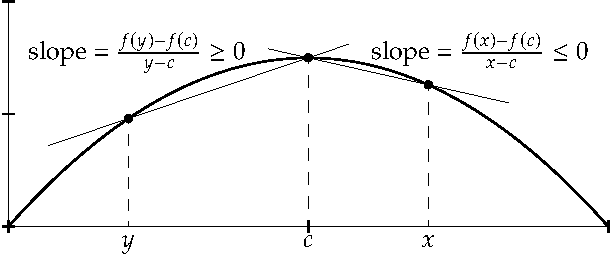
\includegraphics{figures/critpt}
\caption{Slopes of secants at a relative maximum.\label{fig:critpt}}
\end{myfigureht}

As $a < c < b$, there exist
sequences $\{ x_n\}$ and $\{ y_n \}$ in $[a,b]$ and within $\delta$ of $c$,
such that $x_n > c$, and
$y_n < c$ for all $n \in \N$, and such that
 $\lim\, x_n = \lim\, y_n = c$.
Since $f$
is differentiable at $c$,
\begin{equation*}
0 \geq \lim_{n\to\infty} \frac{f(x_n)-f(c)}{x_n-c} 
=
f'(c)
=
\lim_{n\to\infty} \frac{f(y_n)-f(c)}{y_n-c} \geq 0.  \qedhere
\end{equation*}
\end{proof}

For a differentiable function, a point where 
$f'(c) = 0$ is called a \emph{\myindex{critical point}}.  When $f$ is not
differentiable at some points,
it is common to also say that $c$ is a critical point
if $f'(c)$ does not exist.
The theorem says that a relative minimum or maximum at an interior point
of an interval must be a critical point.
As you remember from calculus, finding minima and maxima of a function can
be done by finding all the critical points together with the endpoints of
the interval and simply checking at which of these points
is the function biggest or smallest.

\subsection{Rolle's theorem}

Suppose a function has the same value at both endpoints of an interval.
Intuitively it ought to attain a minimum or a maximum in the interior of the
interval,
then at such a minimum or a maximum, the derivative should be zero.
See \figureref{rollefig} for the geometric idea.  This is the content of the
so-called Rolle's theorem%
\footnote{Named after the French mathematician
\href{https://en.wikipedia.org/wiki/Michel_Rolle}{Michel Rolle}
(1652--1719).}.

\begin{myfigureht}
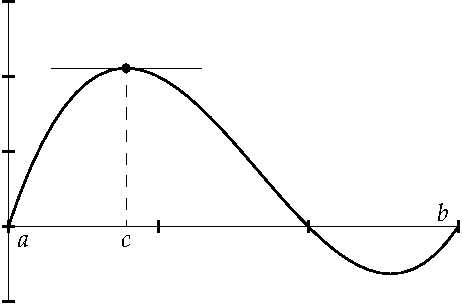
\includegraphics{figures/rollefig}
\caption{Point where the tangent line is horizontal, that is $f'(c) =
0$.\label{rollefig}}
\end{myfigureht}

\begin{thm}[Rolle] \label{thm:rolle}
\index{Rolle's theorem}
Let $f \colon [a,b] \to \R$ be continuous function
differentiable on $(a,b)$ such that $f(a) = f(b)$.
Then there exists a $c \in (a,b)$ such that $f'(c) = 0$.
\end{thm}

\begin{proof}
As $f$ is continuous on $[a,b]$, it attains an absolute minimum and an
absolute 
maximum in $[a,b]$.  We wish to apply \lemmaref{relminmax:lemma}, and
so we need to find some $c \in (a,b)$ where $f$ attains a minimum or a
maximum.
Write $K := f(a) = f(b)$.
If there exists an $x$ such that $f(x) > K$, then the absolute
maximum is bigger than $K$ and hence occurs at some $c \in (a,b)$, and
therefore $f'(c) = 0$.  On the other hand, if there exists an $x$
such that $f(x) < K$, then the absolute minimum occurs at some
$c \in (a,b)$, and so $f'(c) = 0$.  If there is no $x$ such that
$f(x) > K$ or
$f(x) < K$, then $f(x) = K$ for all $x$ and then
$f'(x) = 0$ for all $x \in [a,b]$, so any $c \in (a,b)$ works.
\end{proof}

It is absolutely necessary for the derivative to exist for all $x
\in (a,b)$.  Consider the function $f(x) := \abs{x}$ on $[-1,1]$.
Clearly $f(-1) = f(1)$, but there is no point $c$ where $f'(c) = 0$.

\subsection{Mean value theorem}

We extend \hyperref[thm:rolle]{Rolle's theorem}
to functions that attain different
values at the endpoints.

\begin{thm}[Mean value theorem] \label{thm:mvt}
\index{mean value theorem}
Let $f \colon [a,b] \to \R$ be a continuous function
differentiable on $(a,b)$.  Then there exists a point $c \in (a,b)$
such that
\begin{equation*}
f(b)-f(a) = f'(c)(b-a) .
\end{equation*}
\end{thm}

For a geometric interpretation of the mean value theorem, see
\figureref{mvtfig}.  The idea is that the value $\frac{f(b)-f(a)}{b-a}$
is the slope of the line between the points $\bigl(a,f(a)\bigr)$
and $\bigl(b,f(b)\bigr)$.
Then $c$ is the point such that $f'(c) = \frac{f(b)-f(a)}{b-a}$, that 
is, the tangent line at the point $\bigl(c,f(c)\bigr)$ has the same slope as the
line between $\bigl(a,f(a)\bigr)$ and $\bigl(b,f(b)\bigr)$.
The theorem follows from \hyperref[thm:rolle]{Rolle's theorem},
by subtracting from $f$ the affine linear function with the derivative
$\frac{f(b)-f(a)}{b-a}$ with the same values at $a$ and $b$ as $f$.
That is, we subtract the function whose graph is the straight line
$\bigl(a,f(a)\bigr)$ and $\bigl(b,f(b)\bigr)$.
Then we are looking for a point where this new
function has derivative zero.

\begin{myfigureht}
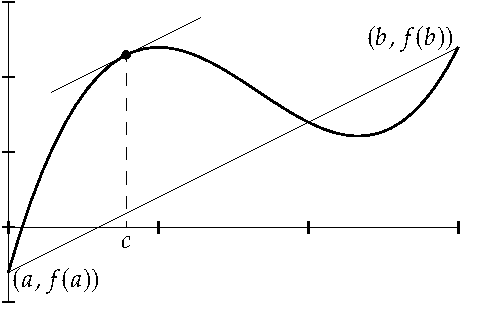
\includegraphics{figures/mvtfig}
\caption{Graphical interpretation of the mean value theorem.\label{mvtfig}}
\end{myfigureht}


\begin{proof}
Define the
function $g \colon [a,b] \to \R$ by
\begin{equation*}
g(x) := f(x)-f(b)-\frac{f(b)-f(a)}{b-a}(x-b) .
\end{equation*}
The function $g$ is differentiable on $(a,b)$,
continuous on $[a,b]$, such that $g(a) = 0$ and $g(b) = 0$.  Thus there exists
a
$c \in (a,b)$ such that $g'(c) = 0$, that is,
\begin{equation*}
0 = g'(c) = f'(c)-\frac{f(b)-f(a)}{b-a} .
\end{equation*}
In other words,
$f'(c)(b-a) = f(b)-f(a)$.
\end{proof}

The proof generalizes.  By considering
$g(x) :=
f(x)-f(b)-\frac{f(b)-f(a)}{\varphi(b)-\varphi(a)}\bigl(\varphi(x)-\varphi(b)\bigr)$,
one can prove the following version.  We leave the proof as an exercise.

\begin{thm}[Cauchy's mean value theorem] \label{thm:cauchymvt}
\index{Cauchy's mean value theorem}
Let $f \colon [a,b] \to \R$ and $\varphi \colon [a,b] \to \R$ be continuous
functions
differentiable on $(a,b)$.  Then there exists a point $c \in (a,b)$
such that
\begin{equation*}
\bigl(f(b)-f(a)\bigr)\varphi'(c) = f'(c)\bigl(\varphi(b)-\varphi(a)\bigr) .
\end{equation*}
\end{thm}

The mean value theorem has the distinction of being one of the few theorems
commonly cited
in court.  That is, when police measure the speed of cars by aircraft, or
via cameras reading license plates, they 
measure the time the car takes to go between two points.
The mean value theorem then
says that the car must have somewhere attained the speed you get by dividing the
difference in distance by the difference in time.



\subsection{Applications}

We now solve our very first differential equation.

\begin{prop} \label{prop:derzeroconst}
Let $I$ be an interval and
let $f \colon I \to \R$ be a differentiable function such that $f'(x) = 0$
for all $x \in I$.
Then $f$ is constant.
\end{prop}

\begin{proof}
Take arbitrary $x,y \in I$ with $x < y$.
Then $f$ restricted to $[x,y]$ satisfies the hypotheses
of the \hyperref[thm:mvt]{mean value theorem}.
Therefore, there is a $c \in (x,y)$ such that
\begin{equation*}
f(y)-f(x) = f'(c)(y-x).
\end{equation*}
As $f'(c) = 0$, we have $f(y) = f(x)$.  Hence,
the function is constant.
\end{proof}

Now that we know what it means for the function to stay constant, let us look
at increasing and decreasing functions.
We say $f \colon I \to \R$ is \emph{\myindex{increasing}}
(resp.\  \emph{\myindex{strictly increasing}}) if
$x < y$ implies $f(x) \leq f(y)$ (resp.\ $f(x) < f(y)$).
We define
\emph{\myindex{decreasing}} and
\emph{\myindex{strictly decreasing}} in the same way by switching the
inequalities for $f$.

\begin{prop} \label{incdecdiffprop}
Let $I$ be an interval and
let $f \colon I \to \R$ be a differentiable function.
%\begin{enumerate}[(i),itemsep=0.5\itemsep,parsep=0.5\parsep,topsep=0.5\topsep,partopsep=0.5\partopsep]
\begin{enumerate}[(i)]
\item $f$ is increasing if and only if $f'(x) \geq 0$ for all $x \in I$.
\item $f$ is decreasing if and only if $f'(x) \leq 0$ for all $x \in I$.
\end{enumerate}
\end{prop}

\begin{proof}
Let us prove the first item.  Suppose $f$ is increasing, then
for all $x,c \in I$ with $x \neq c$, we have
\begin{equation*}
\frac{f(x)-f(c)}{x-c} \geq 0 .
\end{equation*}
Taking a limit as $x$ goes to $c$ we see that $f'(c) \geq 0$.

For the other direction, suppose $f'(x) \geq 0$ for all $x \in I$.
Take any $x, y \in I$ where $x < y$.  By the \hyperref[thm:mvt]{mean value
theorem}, there is some $c \in
(x,y)$ such that
\begin{equation*}
f(y)-f(x) = f'(c)(y-x) .
\end{equation*}
As $f'(c) \geq 0$, and $y-x > 0$, then $f(y) - f(x) \geq 0$ or $f(x) \leq
f(y)$ and so
$f$ is increasing.

We leave the decreasing part to the reader as exercise.
\end{proof}

A similar but weaker statement is true for strictly increasing and
decreasing functions.

\begin{prop} \label{incdecdiffstrictprop}
Let $I$ be an interval and
let $f \colon I \to \R$ be a differentiable function.
\begin{enumerate}[(i)]
\item
\label{incdecdiffstrictprop:i}
If $f'(x) > 0$ for all $x \in I$, then
$f$ is strictly increasing.
\item
\label{incdecdiffstrictprop:ii}
If $f'(x) < 0$ for all $x \in I$,
then $f$ is strictly decreasing.
\end{enumerate}
\end{prop}

The proof of
\ref{incdecdiffstrictprop:i}
is left as an exercise.
Then \ref{incdecdiffstrictprop:ii}
follows from 
\ref{incdecdiffstrictprop:i} by considering $-f$
instead.
The converse of this proposition is not true.  The function
$f(x) := x^3$ is strictly increasing, but $f'(0) = 0$.

\medskip

Another application of the \hyperref[thm:mvt]{mean value theorem} is the following result about
location of extrema, sometimes called the \emph{\myindex{first derivative
test}}.  The theorem is stated for an absolute minimum and
maximum. To apply it to find relative minima
and maxima, restrict $f$ to an interval $(c-\delta,c+\delta)$.

\begin{prop} \label{firstderminmaxtest}
Let $f \colon (a,b) \to \R$ be continuous.  Let $c \in (a,b)$
and suppose
$f$ is differentiable on $(a,c)$ and $(c,b)$.
\begin{enumerate}[(i)]
\item If $f'(x) \leq 0$ for $x \in (a,c)$ and
 $f'(x) \geq 0$ for $x \in (c,b)$, then $f$ has an absolute minimum 
at $c$.
\item If $f'(x) \geq 0$ for $x \in (a,c)$ and
 $f'(x) \leq 0$ for $x \in (c,b)$, then $f$ has an absolute maximum
at $c$.
\end{enumerate}
\end{prop}

\begin{proof}
We prove the first item and leave the second to the reader.
Take $x \in (a,c)$
and a sequence $\{ y_n\}$ such that $x < y_n < c$ for all $n$ and $\lim\, y_n = c$.
By the preceding proposition,
$f$ is decreasing on $(a,c)$ so $f(x) \geq f(y_n)$.
As $f$ is
continuous at $c$, we take the limit to get
$f(x) \geq f(c)$ for all $x \in (a,c)$.

Similarly, take $x \in (c,b)$
and $\{ y_n\}$ a sequence such that $c < y_n < x$ and $\lim\, y_n = c$.
The function is increasing on $(c,b)$ so $f(x) \geq f(y_n)$.
By continuity of $f$ we get
$f(x) \geq f(c)$ for all $x \in (c,b)$.  Thus $f(x) \geq f(c)$ for all
$x \in (a,b)$.
\end{proof}

The converse of the proposition does not hold.  See
\exampleref{baddifffunc:example} below.

\medskip

Another often used application of the mean value theorem you have possibly
seen in calculus is the following result on differentiability at the
end points of an interval.  The proof is
\exerciseref{exercise:endpointderivative}.

\begin{prop} \label{prop:endpointderivative}
\leavevmode
\begin{enumerate}[(i)]
\item
Suppose $f \colon [a,b) \to \R$ is continuous, differentiable in $(a,b)$,
and $\lim_{x \to a} f'(x) = L$.  Then $f$ is differentiable at $a$ and
$f'(a) = L$.
\item
Suppose $f \colon (a,b] \to \R$ is continuous, differentiable in $(a,b)$,
and $\lim_{x \to b} f'(x) = L$.  Then $f$ is differentiable at $b$ and
$f'(b) = L$.
\end{enumerate}
\end{prop}

In fact, using the extension result \propref{context:prop}, you do not need to assume
that $f$ is defined at the end point.  See \exerciseref{exercise:extendboundedder}.

\subsection{Continuity of derivatives and the intermediate value theorem}

Derivatives of functions satisfy an
intermediate value property.

\begin{thm}[Darboux] \label{thm:darboux} \index{Darboux's theorem}
Let $f \colon [a,b] \to \R$ be differentiable.  Suppose $y \in \R$ is such
that $f'(a) < y < f'(b)$ or
$f'(a) > y > f'(b)$.  Then there exists a $c \in (a,b)$ such that $f'(c) =
y$.
\end{thm}

The proof follows by subtracting $f$ and a linear function with derivative
$y$.  The new function $g$ reduces the problem
to the case $y=0$, where $g'(a) > 0 > g'(b)$.  That is, $g$ is increasing at $a$ and
decreasing at $b$, so it must attain a maximum inside $(a,b)$,
where the derivative is zero.  See \figureref{darbouxthmfig}.

\begin{myfigureht}
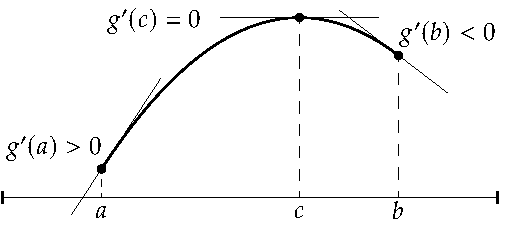
\includegraphics{figures/darbouxthmfig}
\caption{Idea of the proof of Darboux theorem.\label{darbouxthmfig}}
\end{myfigureht}

\begin{proof}
Suppose 
$f'(a) < y < f'(b)$.
Define
\begin{equation*}
g(x) := yx - f(x) .
\end{equation*}
The function $g$ is continuous on $[a,b]$, and so $g$ attains a maximum at some $c \in
[a,b]$.

The function $g$ is also differentiable on $[a,b]$.
Compute $g'(x) = y-f'(x)$.  Thus $g'(a) > 0$.  As the derivative is
the limit of difference quotients and is positive, there must be some
difference quotient that is positive.  That is, there must exist
an $x > a$ such that
\begin{equation*}
\frac{g(x)-g(a)}{x-a} > 0 ,
\end{equation*}
or $g(x) > g(a)$.  Thus $g$
cannot possibly have a maximum at $a$.  Similarly, as $g'(b) < 0$,
we find an $x < b$ (a different $x$) such that
$\frac{g(x)-g(b)}{x-b} < 0$ or that $g(x) > g(b)$, thus
$g$ cannot possibly have a maximum at $b$.
Therefore, $c \in (a,b)$,
and \lemmaref{relminmax:lemma} applies: As $g$ attains a maximum
at $c$ we find $g'(c) = 0$
and so $f'(c) = y$.

Similarly, if $f'(a) > y > f'(b)$, consider $g(x) := f(x)- yx$.
\end{proof}

We have seen already that
there exist discontinuous functions that have the
intermediate value property.  While it is hard to imagine at first, there
also
exist functions that are differentiable everywhere and the derivative is not
continuous.

\begin{example} \label{baddifffunc:example}
Let $f \colon \R \to \R$ be the function defined by
\begin{equation*}
f(x) :=
\begin{cases}
{\bigl( x \sin(\nicefrac{1}{x}) \bigr)}^2 & \text{if } x \not= 0, \\
0 & \text{if } x = 0.
\end{cases}
\end{equation*}
We claim that $f$ is differentiable everywhere, but
$f' \colon \R \to \R$ is not continuous at
the origin.  Furthermore, $f$ has a minimum at 0, but the derivative
changes sign infinitely often near the origin.
See \figureref{fig:nonc1diff}.
\begin{myfigureht}
\subimport*{figures/}{nonc1diff_full.pdf_t}
\caption{A function with a discontinuous derivative. The function $f$ is on the left
and $f'$ is on the right.  Notice that $f(x) \leq x^2$ on the left graph.\label{fig:nonc1diff}}
\end{myfigureht}

Proof: It is immediate from the definition that $f$ has an absolute
minimum at 0: we know $f(x) \geq 0$ for all $x$ and $f(0) = 0$.

The function $f$ is differentiable for $x\not=0$,
and
the derivative 
is $2 \sin (\nicefrac{1}{x}) \bigl( x \sin (\nicefrac{1}{x}) -
\cos(\nicefrac{1}{x}) \bigr)$.
As an exercise, show that for $x_n = \frac{4}{(8n+1)\pi}$,
we have
$\lim\, f'(x_n) = -1$, and for
$y_n = \frac{4}{(8n+3)\pi}$, we have
$\lim\, f'(y_n) = 1$.  Hence if $f'$ exists at $0$,
then it cannot be continuous.

Let us show that $f'$ exists at 0.  We claim that the derivative is zero.
In other words $\abs{\frac{f(x)-f(0)}{x-0} - 0}$ goes to zero
as $x$ goes to zero.  For $x \not= 0$, we have
\begin{equation*}
\abs{\frac{f(x)-f(0)}{x-0} - 0}
=
\abs{\frac{x^2 \sin^2(\nicefrac{1}{x})}{x}}
=
\abs{x \sin^2(\nicefrac{1}{x})}
\leq
\abs{x} .
\end{equation*}
And, of course, as $x$ tends to zero, then $\abs{x}$ tends to zero and hence
$\abs{\frac{f(x)-f(0)}{x-0} - 0}$ goes to zero.  Therefore, $f$
is differentiable at 0 and the derivative at 0 is 0.
A key point in the calculation above
is that $\abs{f(x)} \leq x^2$,
see also Exercises \ref{exercise:bndmuldiff} and
\ref{exercise:diffsqueeze}.
\end{example}

It is sometimes useful to assume the derivative of a differentiable
function is continuous.  If $f \colon I \to \R$ is differentiable and
the derivative $f'$ is continuous on $I$, then we say $f$ is
\emph{\myindex{continuously
differentiable}}\index{differentiable!continuously}.  It is common to
write $C^1(I)$ for the set of continuously differentiable functions on $I$.

\subsection{Exercises}

\begin{exercise}
Finish the proof of \propref{incdecdiffprop}.
\end{exercise}

\begin{exercise}
Finish the proof of \propref{firstderminmaxtest}.
\end{exercise}

\begin{exercise} \label{exercise:boundeddermeanslip}
Suppose $f \colon \R \to \R$ is a differentiable
function such that $f'$ is a bounded function.  Prove
that $f$ is a Lipschitz continuous function.
\end{exercise}

\pagebreak[1]
\begin{exercise}
Suppose $f \colon [a,b] \to \R$ is differentiable and $c \in [a,b]$.
Show there exists a sequence $\{ x_n \}$ converging to $c$, $x_n
\not= c$ for all $n$, such that
\begin{equation*}
f'(c) = \lim_{n\to \infty} f'(x_n).
\end{equation*}
Do note this does \emph{not} imply that $f'$ is continuous (why?).
\end{exercise}

\pagebreak[1]
\begin{exercise}
Suppose $f \colon \R \to \R$ is a function such that
$\abs{f(x)-f(y)} \leq \abs{x-y}^2$ for all $x$ and $y$.  Show that
$f(x) = C$ for some constant $C$.  Hint: Show that $f$ is differentiable
at all points and compute the derivative.
\end{exercise}

\begin{exercise} \label{exercise:posderincr}
Finish the proof of \propref{incdecdiffstrictprop}.  That is,
suppose $I$ is an interval and
$f \colon I \to \R$ is a differentiable function such that
$f'(x) > 0$ for all $x \in I$.
Show that $f$ is strictly increasing.
\end{exercise}

\begin{exercise}
Suppose $f \colon (a,b) \to \R$ is a differentiable function
such that
$f'(x) \not= 0$ for all $x \in (a,b)$.  Suppose there
exists
a point $c \in (a,b)$ such that $f'(c) > 0$.
Prove $f'(x) > 0$ for all $x \in (a,b)$.
\end{exercise}

\begin{exercise} \label{exercise:samediffconst}
Suppose $f \colon (a,b) \to \R$ and $g \colon (a,b) \to \R$ are
differentiable functions such that $f'(x) = g'(x)$ for all $x \in (a,b)$,
then show that there exists a constant $C$ such that $f(x) = g(x) + C$.
\end{exercise}

\begin{exercise}
Prove the following version of \myindex{L'H\^opital's rule}\index{L'Hospital's rule}.
Suppose 
$f \colon (a,b) \to \R$ and $g \colon (a,b) \to \R$ are differentiable
functions and $c \in (a,b)$.  Suppose that $f(c) = 0$, $g(c)=0$,
$g'(x) \not= 0$ when $x \not= c$, and
that the limit of $\nicefrac{f'(x)}{g'(x)}$ as $x$ goes to $c$ exists.  Show that
\begin{equation*}
\lim_{x \to c} \frac{f(x)}{g(x)} = 
\lim_{x \to c} \frac{f'(x)}{g'(x)} .
\end{equation*}
Compare to \exerciseref{exercise:simpleLHopital}.
\end{exercise}

\begin{exercise}
Let $f \colon (a,b) \to \R$ be an unbounded differentiable function.  Show
$f' \colon (a,b) \to \R$ is unbounded.
\end{exercise}

\begin{exercise}
Prove the theorem Rolle actually proved in 1691:
\emph{If $f$ is a polynomial,
$f'(a) = f'(b) = 0$ for some $a < b$,
and there is no $c \in (a,b)$ such that $f'(c) = 0$,
then there is at most one root of $f$ in $(a,b)$,
that is at most one $x \in (a,b)$ such that $f(x) = 0$.}
In other words, between any two consecutive roots of $f'$ is at most one
root of $f$.
Hint: Suppose there are two roots and see what happens.
\end{exercise}

\begin{exercise}
Suppose $a,b \in \R$ and $f \colon \R \to \R$ is differentiable,
$f'(x) = a$ for all $x$, and $f(0) = b$.  Find $f$ and prove that 
it is the unique differentiable function with this property.
\end{exercise}

\begin{exercise} \label{exercise:endpointderivative}
\leavevmode
\begin{enumerate}[a)]
\item
Prove \propref{prop:endpointderivative}.
\item 
Suppose $f \colon (a,b) \to \R$ is continuous, and suppose $f$ is differentiable everywhere except at $c \in
(a,b)$ and $\lim_{x \to c} f'(x) = L$.
Prove that $f$ is differentiable at
$c$ and $f'(c) = L$.
\end{enumerate}
\end{exercise}

\begin{exercise} \label{exercise:extendboundedder}
Suppose $f \colon (0,1) \to \R$ is differentiable and $f'$
is bounded.
\begin{enumerate}[a)]
\item
Show that there exists a continuous function $g \colon [0,1) \to \R$
such that $f(x) = g(x)$ for all $x \not= 0$.\\
Hint: \propref{context:prop} and
\exerciseref{exercise:boundeddermeanslip}.
\item
Find an example where the $g$ is not differentiable at $x=0$.
\\
Hint: Consider something based on $\sin(\ln x)$,
and assume you know basic properties of
$\sin$ and $\ln$ from calculus.
\item
Instead of assuming that $f'$ is bounded, assume that $\lim_{x \to 0} f'(x)
= L$.  Prove that not only does $g$ exist but it is differentiable at $0$
and $g'(0) = L$.
\end{enumerate}
\end{exercise}

\begin{exercise}
Prove \thmref{thm:cauchymvt}.
\end{exercise}

%%%%%%%%%%%%%%%%%%%%%%%%%%%%%%%%%%%%%%%%%%%%%%%%%%%%%%%%%%%%%%%%%%%%%%%%%%%%%%

\sectionnewpage
\section{Taylor's theorem}
\label{sec:taylor}

\sectionnotes{less than a lecture (optional section)}

\subsection{Derivatives of higher orders}

When $f \colon I \to \R$ is differentiable, we obtain a function
$f' \colon I \to \R$.  The function
$f'$ is called the \emph{\myindex{first derivative}} of $f$.
If $f'$ is differentiable, we denote by
$f'' \colon I \to \R$ the derivative of $f'$.  The function $f''$
is called the \emph{\myindex{second derivative}} of $f$.
\glsadd{not:secondthirdfourthder}
We similarly obtain
$f'''$, $f''''$, and so on.
With a larger number of derivatives
the notation would get out of hand; we denote
by $f^{(n)}$ the
\glsadd{not:nthder}
\emph{$n$th derivative}\index{nth derivative@$n$th derivative} of $f$.

When $f$ possesses $n$ derivatives, we say $f$ is
\emph{$n$ times differentiable}\index{n times differentiable@$n$ times
differentiable}\index{differentiable!n times@$n$ times}.

\subsection{Taylor's theorem}

Taylor's theorem%
\footnote{Named for the English mathematician
\href{https://en.wikipedia.org/wiki/Brook_Taylor}{Brook Taylor}
(1685--1731).
It was first found by
the Scottish mathematician
\href{https://en.wikipedia.org/wiki/James_Gregory_(mathematician)}{James Gregory}
(1638--1675).  The statement we give
was proved by
\href{https://en.wikipedia.org/wiki/Lagrange}{Joseph-Louis Lagrange}
(1736--1813)}
is a generalization of the \hyperref[thm:mvt]{mean value theorem}.
Mean value theorem says that up to a small error $f(x)$ for $x$ near $x_0$ can be
approximated by $f(x_0)$, that is
\begin{equation*}
f(x) = f(x_0) + f'(c)(x-x_0),
\end{equation*}
where the \myquote{error} is measured in terms of the first derivative
at some point $c$ between $x$ and $x_0$.
Taylor's theorem generalizes this result to higher derivatives.
It tells us that up to a small error, any $n$
times differentiable function can be approximated at a point $x_0$
by a polynomial.  The
error of this approximation behaves like ${(x-x_0)}^{n}$ near the point $x_0$.
To see why this is a good approximation notice that for a big $n$, 
${(x-x_0)}^n$ is very small in a small interval around $x_0$.

\begin{defn}
For an $n$ times differentiable function $f$ defined near a point $x_0 \in \R$, define the
$n$th order \emph{\myindex{Taylor polynomial}}%
\index{nth order Taylor polynomial@$n$th order Taylor polynomial}
for $f$ at $x_0$ as
\begin{equation*}
\begin{split}
P_n^{x_0}(x)
& :=
\sum_{k=0}^n
\frac{f^{(k)}(x_0)}{k!}{(x-x_0)}^k
\\
& =
f(x_0)
+ f'(x_0)(x-x_0)
+ \frac{f''(x_0)}{2}{(x-x_0)}^2
+ \frac{f^{(3)}(x_0)}{6}{(x-x_0)}^3
+ \cdots
+ \frac{f^{(n)}(x_0)}{n!}{(x-x_0)}^n .
\end{split}
\end{equation*}
\end{defn}

See \figureref{fig:taylorsin} for
the odd degree Taylor polynomials for the sine function at $x_0=0$.
The even degree terms are all zero, as even derivatives 
of sine are again a sine, which are zero at the origin.
\begin{myfigureht}
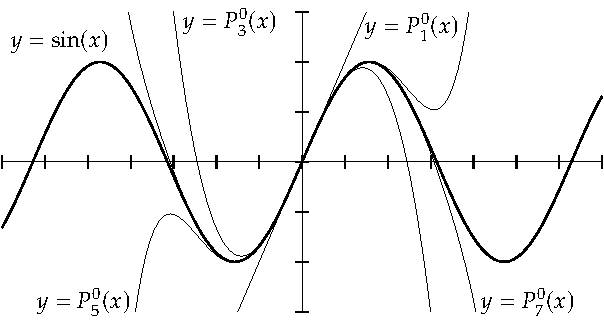
\includegraphics{figures/taylorsin}
\caption{The odd degree Taylor polynomials for the sine
function.\label{fig:taylorsin}}
\end{myfigureht}

Taylor's theorem says a function behaves like its $n$th
Taylor polynomial.  The 
\hyperref[thm:mvt]{mean value theorem} is really Taylor's theorem
for the first derivative.

\begin{thm}[Taylor]\index{Taylor's theorem} \label{thm:taylor}
Suppose $f \colon [a,b] \to \R$ is a function with $n$ continuous
derivatives on $[a,b]$ and such that $f^{(n+1)}$ exists on $(a,b)$.
Given distinct points $x_0$ and $x$ in $[a,b]$,
we can find a point $c$ between $x_0$
and $x$ such that
\begin{equation*}
f(x)=P_{n}^{x_0}(x)+\frac{f^{(n+1)}(c)}{(n+1)!}{(x-x_0)}^{n+1} .
\end{equation*}
\end{thm}

The term $R_n^{x_0}(x):=\frac{f^{(n+1)}(c)}{(n+1)!}{(x-x_0)}^{n+1}$ is called the
\emph{remainder term}\index{remainder term in Taylor's formula}.  This
form 
of the remainder term is called the
\emph{\myindex{Lagrange form}} of the remainder.  There are other ways
to write the remainder term, but we skip those.  Note that $c$ depends on
both $x$ and $x_0$.

\begin{proof}
Find a number $M_{x,x_0}$ (depending on $x$ and $x_0$) solving the equation
\begin{equation*}
f(x)=P_{n}^{x_0}(x)+M_{x,x_0}{(x-x_0)}^{n+1} .
\end{equation*}
Define a function $g(s)$ by
\begin{equation*}
g(s) := f(s)-P_n^{x_0}(s)-M_{x,x_0}{(s-x_0)}^{n+1} .
\end{equation*}
We compute
the $k$th derivative at $x_0$ of the Taylor polynomial
${(P_n^{x_0})}^{(k)}(x_0) = f^{(k)}(x_0)$ for
$k=0,1,2,\ldots,n$ (the zeroth derivative of a function is the function
itself).  Therefore,
\begin{equation*}
g(x_0) = g'(x_0) = g''(x_0) = \cdots = g^{(n)}(x_0) = 0 .
\end{equation*}
In particular, $g(x_0) = 0$.
On the other hand $g(x) = 0$.  By the
\hyperref[thm:mvt]{mean value theorem}
there exists an $x_1$ between $x_0$ and $x$ such that $g'(x_1) = 0$.
Applying the \hyperref[thm:mvt]{mean value theorem}
to $g'$ we obtain that there exists
$x_2$ between $x_0$ and $x_1$ (and therefore between $x_0$ and $x$)
such that $g''(x_2) = 0$.  We repeat the
argument $n+1$ times to obtain a number $x_{n+1}$ between $x_0$ and $x_n$
(and therefore between $x_0$ and $x$) such that $g^{(n+1)}(x_{n+1}) = 0$.

Let $c:=x_{n+1}$.
We compute the $(n+1)$th derivative of $g$ to find
\begin{equation*}
g^{(n+1)}(s) = f^{(n+1)}(s)-(n+1)!\,M_{x,x_0} .
\end{equation*}
Plugging in $c$ for $s$ we obtain $M_{x,x_0} = \frac{f^{(n+1)}(c)}{(n+1)!}$, and
we are done.
\end{proof}

In the proof, we have computed 
${(P_n^{x_0})}^{(k)}(x_0) = f^{(k)}(x_0)$ for $k=0,1,2,\ldots,n$.
Therefore, the Taylor polynomial has the same derivatives as $f$ at $x_0$
up to the $n$th derivative.  That is why the Taylor polynomial is
a good approximation to $f$.
Notice how in \figureref{fig:taylorsin} the Taylor polynomials are
reasonably good approximations to the sine near $x=0$.

We do not necessarily get good approximations
by the Taylor polynomial everywhere.
Consider expanding the function $f(x) :=
\frac{x}{1-x}$ around 0, for $x < 1$, we get the graphs in
\figureref{fig:taylorgeom}.  The dotted lines are the first, second, and
third degree approximations.  The dashed line is
the 20th degree polynomial, and yet the approximation only seems to get
better with the degree for $x > -1$, and for smaller $x$, it in fact gets worse.
The polynomials
are the partial sums of the geometric series $\sum_{n=1}^\infty x^n$,
and the series only converges on $(-1,1)$.
See the discussion of power series
\sectionref{sec:moreonseries}.

\begin{myfigureht}
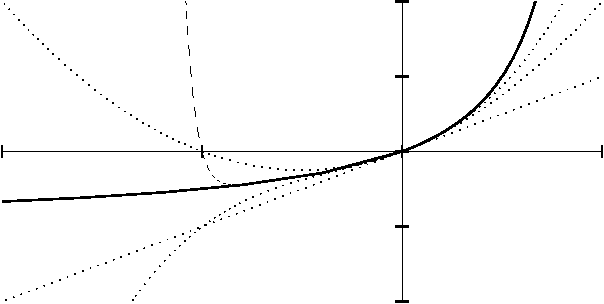
\includegraphics{figures/taylorgeom}
\caption{The function $\frac{x}{1-x}$, and the Taylor polynomials
$P_1^0$, $P_2^0$, $P_3^0$ (all dotted), and the polynomial $P_{20}^0$
(dashed).\label{fig:taylorgeom}}
\end{myfigureht}

If $f$ is \emph{\myindex{infinitely
differentiable}}\index{differentiable!infinitely},
that is, if $f$ can be
differentiated any number of times, then 
we define the \emph{\myindex{Taylor series}}:
\begin{equation*}
%T^{x_0}(x)
%:=
\sum_{k=0}^\infty
\frac{f^{(k)}(x_0)}{k!}{(x-x_0)}^k .
\end{equation*}
There is no guarantee that this series converges for any
$x \not= x_0$.  And even where it does converge, there is no guarantee
that it converges to the function $f$.  Functions $f$
whose Taylor series at every point $x_0$
converges to $f$ in some open interval containing $x_0$
are called
\emph{analytic functions}\index{analytic function}.
Most functions one tends to see in practice are analytic.
See \exerciseref{exercise:nonanalytic}, for an example of a non-analytic
function.

\medskip

The definition of derivative says that
a function is
differentiable if it
is locally approximated by a line.
We mention in passing that there exists a converse to Taylor's
theorem,
which we will neither state nor prove,
saying that if a function is
locally approximated in a certain way by a polynomial of degree $d$, then it
has $d$ derivatives.

\medskip

Taylor's theorem gives us a quick proof of a version of
the second derivative test.
By a \emph{\myindex{strict relative minimum}}\index{minimum!strict relative}
of $f$ at $c$,
we mean that there exists a $\delta > 0$ such that $f(x) > f(c)$ for
all $x \in (c-\delta,c+\delta)$ where $x\not=c$.
A \emph{\myindex{strict relative maximum}}\index{maximum!strict relative}
is defined similarly.
Continuity of the second derivative is not needed, but the proof is more
difficult and is left as an exercise.  The proof also generalizes
immediately into the $n$th derivative test, which is also left as
an exercise.

\begin{prop}[Second derivative test]\index{second derivative test}
Suppose $f \colon (a,b) \to \R$ is twice continuously differentiable,
$x_0 \in (a,b)$, $f'(x_0) = 0$ and $f''(x_0) > 0$.  Then $f$ has a strict relative
minimum at $x_0$.
\end{prop}

\begin{proof}
As $f''$ is continuous, there exists a $\delta > 0$
such that $f''(c) > 0$ for all $c \in (x_0-\delta,x_0+\delta)$,
see \exerciseref{exercise:positivecontneigh}.
Take $x \in (x_0-\delta,x_0+\delta)$, $x \not= x_0$.
Taylor's theorem says that for some $c$ between $x_0$ and $x$,
\begin{equation*}
f(x) 
=
f(x_0) + f'(x_0) (x-x_0) +
\frac{f''(c)}{2}{(x-x_0)}^{2} 
=
f(x_0) + \frac{f''(c)}{2}{(x-x_0)}^{2}  .
\end{equation*}
As $f''(c) > 0$, and ${(x-x_0)}^2 > 0$, then $f(x) > f(x_0)$.
\end{proof}

\subsection{Exercises}

\begin{exercise}
Compute the $n$th Taylor Polynomial at $0$ for the exponential function.
\end{exercise}

\begin{exercise}
Suppose $p$ is a polynomial of degree $d$.  Given $x_0 \in \R$,
show that
the $(d+1)$th Taylor polynomial for $p$ at $x_0$ is equal to $p$.
\end{exercise}

\begin{exercise}
Let $f(x) := \abs{x}^3$.  Compute $f'(x)$ and $f''(x)$ for all $x$,
but show that $f^{(3)}(0)$ does not exist.
\end{exercise}

\begin{exercise}
Suppose $f \colon \R \to \R$ has $n$ continuous derivatives.  Show
that for every $x_0 \in \R$,
there exist polynomials $P$ and $Q$ of degree $n$ and 
an $\epsilon > 0$ such that $P(x) \leq f(x) \leq Q(x)$ for all $x \in
[x_0,x_0+\epsilon]$  and
$Q(x)-P(x) = \lambda {(x-x_0)}^n$ for some $\lambda \geq 0$.
\end{exercise}

\begin{exercise}
If $f \colon [a,b] \to \R$ has $n+1$ continuous derivatives
and $x_0 \in [a,b]$,
prove
$\lim\limits_{x\to x_0} \frac{R_n^{x_0}(x)}{{(x-x_0)}^n} = 0$.
\end{exercise}

\begin{exercise}
Suppose $f \colon [a,b] \to \R$ has $n+1$ continuous derivatives
and $x_0 \in (a,b)$.
Prove: $f^{(k)}(x_0) = 0$ for all $k = 0, 1, 2, \ldots, n$
if and only if $g(x) := \frac{f(x)}{{(x-x_0)}^{n+1}}$ is continuous at $x_0$.
\end{exercise}

\begin{exercise}
Suppose $a,b,c \in \R$ and $f \colon \R \to \R$ is differentiable,
$f''(x) = a$ for all $x$, $f'(0) = b$, and $f(0) = c$.  Find $f$ and prove that 
it is the unique differentiable function with this property.
\end{exercise}

\begin{exercise}[Challenging]
Show that a simple converse to Taylor's theorem does not hold.
Find a function $f \colon \R \to \R$ with no second derivative at $x=0$ such that
$\abs{f(x)} \leq \abs{x^3}$, that is, $f$ goes to zero at 0 faster than $x^3$, and
while $f'(0)$ exists, $f''(0)$ does not.
\end{exercise}

\begin{exercise} \label{exercise:extendboundedder2}
Suppose $f \colon (0,1) \to \R$ is differentiable and $f''$
is bounded.
\begin{enumerate}[a)]
\item
Show that there exists a once differentiable function $g \colon [0,1) \to \R$
such that $f(x) = g(x)$ for all $x \not= 0$.  Hint: 
See
\exerciseref{exercise:extendboundedder}.
\item
Find an example where the $g$ is not twice differentiable at $x=0$.
\end{enumerate}
\end{exercise}

\begin{exercise}
Prove the
\emph{$n$th derivative test}\index{nth derivative test@$n$th derivative test}.
Suppose $n \in \N$,
$x_0 \in (a,b)$, and $f \colon (a,b) \to \R$ is $n$ times continuously
differentiable, with $f^{(k)}(x_0) = 0$ for $k=1,2,\ldots,n-1$, and
$f^{(n)}(x_0)
\not= 0$.
Prove:
\begin{enumerate}[a)]
\item
If $n$ is odd, then $f$ has neither a relative minimum,
nor a maximum at $x_0$.
\item
If $n$ is even, then $f$ has a strict relative minimum at $x_0$ if
$f^{(n)}(x_0) > 0$
and a strict relative maximum at $x_0$ if $f^{(n)}(x_0) < 0$.
\end{enumerate}
\end{exercise}

\begin{exercise}
Prove the more general version of the second derivative test.
Suppose $f \colon (a,b) \to \R$ is differentiable and $x_0 \in (a,b)$
is such that, $f'(x_0) = 0$, $f''(x_0)$ exists, and $f''(x_0) > 0$.
Prove that $f$ has a strict relative
minimum at $x_0$.  Hint: Consider the limit definition of $f''(x_0)$.
\end{exercise}

%%%%%%%%%%%%%%%%%%%%%%%%%%%%%%%%%%%%%%%%%%%%%%%%%%%%%%%%%%%%%%%%%%%%%%%%%%%%%%

\sectionnewpage
\section{Inverse function theorem}
\label{sec:ift}

\sectionnotes{less than 1 lecture (optional section, needed for
\sectionref{sec:logandexp}, requires 
\sectionref{sec:monotonefunc})}

\subsection{Inverse function theorem}

We start with a simple example.  Consider the function $f(x) := a x$ for a
number $a \not= 0$.  Then $f \colon \R \to \R$ is bijective, and the inverse
is $f^{-1}(y) = \frac{1}{a} y$.  In particular, $f'(x) = a$ and 
$(f^{-1})'(y) = \frac{1}{a}$.  As differentiable functions are
\myquote{infinitesimally like} linear functions, we expect the same
behavior from the inverse function.
The main idea of differentiating inverse functions is the following lemma.

\begin{lemma} \label{lemma:ift}
Let $I,J \subset \R$ be intervals.
If $f \colon I \to J$ is strictly monotone (hence one-to-one),
onto ($f(I) = J$),
differentiable at $x_0 \in I$, and $f'(x_0) \not= 0$,
then the inverse 
$f^{-1}$ is differentiable at $y_0 = f(x_0)$ and
\begin{equation*}
(f^{-1})'(y_0) = \frac{1}{f'\bigl( f^{-1}(y_0) \bigr)} = \frac{1}{f'(x_0)} .
\end{equation*}
If $f$ is continuously differentiable and $f'$ is never zero, then $f^{-1}$
is continuously differentiable.
\end{lemma}

\begin{proof}
By \propref{prop:invcont}, $f$ has a continuous inverse.  For convenience
call the inverse $g \colon J \to I$.
Let $x_0,y_0$ be as in the statement.  For $x \in I$ write $y := f(x)$.
If $x \not= x_0$ and so $y \not= y_0$, we find
\begin{equation*}
\frac{g(y)-g(y_0)}{y-y_0} =
\frac{g\bigl(f(x)\bigr)-g\bigl(f(x_0)\bigr)}{f(x)-f(x_0)} =
\frac{x-x_0}{f(x)-f(x_0)} .
\end{equation*}
See \figureref{inversefig} for the geometric idea.
\begin{myfigureht}
\subimport*{figures/}{inversefigAB.pdf_t}
\caption{Interpretation of the derivative of the inverse
function.\label{inversefig}}
\end{myfigureht}

Let
\begin{equation*}
Q(x) :=
\begin{cases}
\frac{x-x_0}{f(x)-f(x_0)} & \text{if } x \neq x_0, \\
\frac{1}{f'(x_0)}         & \text{if } x = x_0 \quad \text{(notice that }
f'(x_0) \neq 0 \text{)}.
\end{cases}
\end{equation*}
As $f$ is differentiable at $x_0$, 
\begin{equation*}
\lim_{x \to x_0} Q(x) =
\lim_{x \to x_0} 
\frac{x-x_0}{f(x)-f(x_0)} 
=
\frac{1}{f'(x_0)}
=
Q(x_0) ,
\end{equation*}
that is, $Q$ is continuous at $x_0$.
As $g(y)$ is continuous at $y_0$,
the composition $Q\bigl(g(y)\bigr) = \frac{g(y)-g(y_0)}{y-y_0}$
is continuous at $y_0$ by
\propref{prop:compositioncont}.
Therefore,
\begin{equation*}
\frac{1}{f'\bigl(g(y_0)\bigr)}
= Q\bigl(g(y_0)\bigr)
= \lim_{y \to y_0} Q\bigl(g(y)\bigr)
= \lim_{y \to y_0} \frac{g(y)-g(y_0)}{y-y_0} .
\end{equation*}
So $g$ is differentiable at $y_0$ and $g'(y_0) =
\frac{1}{f'\left(\vphantom{1^1_1}g(y_0)\right)}$.

If $f'$ is continuous and nonzero at all $x \in I$,
then the lemma applies at all $x \in I$.  As $g$ is also
continuous (it is differentiable), the derivative $g'(y) =
\frac{1}{f'\left(\vphantom{1^1_1}g(y)\right)}$ must be continuous.
\end{proof}

What is usually called the inverse function theorem is the following result.

\begin{thm}[Inverse function theorem]\index{inverse function theorem}
Let $f \colon (a,b) \to \R$ be a continuously differentiable function,
$x_0 \in (a,b)$ a point where $f'(x_0) \not= 0$.  Then there exists
an open interval $I \subset (a,b)$ with $x_0 \in I$, the
restriction $f|_{I}$ is injective with a continuously differentiable inverse
$g \colon J \to I$ defined on an interval $J := f(I)$,
and
\begin{equation*}
g'(y) = \frac{1}{f'\bigl( g(y) \bigr)} \qquad \text{for all } y \in J.
\end{equation*}
\end{thm}

\begin{proof}
Without loss of generality, suppose $f'(x_0) > 0$.  As $f'$ is
continuous, there must exist an open interval $I = (x_0-\delta,x_0+\delta)$ 
such that $f'(x) > 0$ for all $x \in I$.  See
\exerciseref{exercise:positivecontneigh}.

By \propref{incdecdiffstrictprop} $f$ is strictly increasing
on $I$, and hence the restriction $f|_{I}$ is bijective onto $J: = f(I)$.
As $f$ is continuous,
then by the
\corref{cor:continterval}
(or directly via the
\hyperref[IVT:thm]{intermediate value theorem})
$f(I)$ is in interval.
Now apply \lemmaref{lemma:ift}.
\end{proof}

If you tried to prove the existence of roots directly as in
\exampleref{example:sqrt2}, you saw
how difficult that endeavor is.  However, with the machinery we have built
for inverse functions it becomes
an almost trivial exercise, and with the lemma above we prove
far more than mere existence.

\begin{cor}
Given $n \in \N$ and $x \geq 0$ there exists a unique 
number $y \geq 0$ (denoted $x^{1/n} := y$), such that $y^n = x$.  Furthermore,
the function $g \colon (0,\infty) \to (0,\infty)$ defined by
$g(x) := x^{1/n}$ is continuously differentiable and
\begin{equation*}
g'(x) = \frac{1}{nx^{(n-1)/n}} = \frac{1}{n} \, x^{(1-n)/n} ,
\end{equation*}
using the convention $x^{m/n} := {(x^{1/n})}^{m}$.
\end{cor}

\begin{proof}
For $x=0$ the existence of a unique root is trivial.

Let $f \colon (0,\infty) \to (0,\infty)$ be defined by $f(y) := y^n$.
The function $f$ is continuously differentiable
and $f'(y) = ny^{n-1}$, see \exerciseref{exercise:diffofxn}.  For $y > 0$ the derivative $f'$ is strictly positive
and so again by \propref{incdecdiffstrictprop}, $f$ is strictly
increasing (this can also be proved directly).
Given any $M > 1$, $f(M) = M^n \geq M$, and given any $1 > \epsilon > 0$,
$f(\epsilon) = \epsilon^n \leq \epsilon$.  For every $x$ with $\epsilon < x <
M$, we have, by the
\hyperref[IVT:thm]{intermediate value theorem}, that $x \in
f\bigl( [\epsilon,M] \bigr) \subset
f\bigl( (0,\infty) \bigr)$.  As $M$ and $\epsilon$ were arbitrary, $f$ is onto
$(0,\infty)$, and hence $f$ is bijective.
Let $g$ be the inverse of $f$, and we obtain
the existence and uniqueness of positive
$n$th roots.  \lemmaref{lemma:ift} says $g$ has a continuous
derivative and $g'(x) =
\frac{1}{f'\left(\vphantom{1^1_1}g(x)\right)} = \frac{1}{n {(x^{1/n})}^{n-1}}$.
\end{proof}

\begin{example}
The corollary provides a good example of where the inverse function theorem
gives us an interval smaller than $(a,b)$.  Take $f \colon \R \to \R$
defined by $f(x) := x^2$.  Then $f'(x) \not= 0$
as long as $x \not= 0$.  If $x_0 > 0$, we can take $I=(0,\infty)$, but
no larger.
\end{example}

\begin{example}
Another useful example is $f(x) := x^3$.  The function $f \colon \R \to \R$ is
one-to-one and onto, so $f^{-1}(y) = y^{1/3}$ exists on the entire real
line including zero and negative $y$.  The function $f$ has
a continuous derivative, but $f^{-1}$ has no derivative at the origin.  The
point is that $f'(0) = 0$.  See \figureref{cubecuberootfig} for a graph,
notice the vertical tangent on the cube root at the origin.
See also \exerciseref{exercise:oddroot}.
\begin{myfigureht}
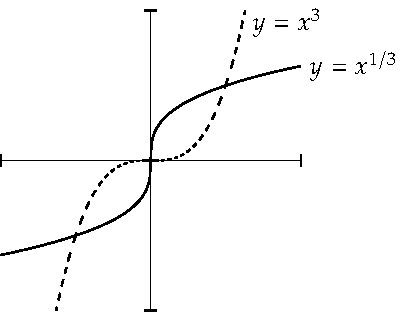
\includegraphics{figures/cubecuberoot}
\caption{Graphs of $x^3$ and $x^{1/3}$.\label{cubecuberootfig}}
\end{myfigureht}
\end{example}


\subsection{Exercises}

\begin{exercise}
Suppose $f \colon \R \to \R$ is continuously differentiable such that
$f'(x) > 0$ for all $x$.  Show that $f$ is invertible on the interval $J =
f(\R)$, the inverse is continuously differentiable, and ${(f^{-1})}'(y) >
0$ for all $y \in f(\R)$.
\end{exercise}

\begin{exercise}
Suppose $I,J$ are intervals and a monotone onto $f \colon I \to J$ has an inverse $g \colon J \to I$.
Suppose you already know that both $f$ and $g$ are differentiable
everywhere and $f'$ is never zero.  Using chain rule but not \lemmaref{lemma:ift} prove the
formula $g'(y) = \frac{1}{f'\left(\vphantom{1_1^1}g(y)\right)}$. % \bigl( \bigr) are overly big here!
\end{exercise}

\begin{exercise}
Let $n\in \N$ be even.
Prove that every $x > 0$ has a unique negative $n$th root.
That is, there exists a negative number $y$ such that $y^n = x$.
Compute the derivative
of the function $g(x) := y$.
\end{exercise}

\begin{exercise} \label{exercise:oddroot}
Let $n \in \N$ be odd and $n \geq 3$.
Prove that every $x$ has a unique $n$th root.
That is, there exists a number $y$ such that $y^n = x$.  Prove that
the function defined by $g(x) := y$ is differentiable except at $x=0$
and compute the derivative.  Prove that $g$ is not differentiable at $x=0$.
\end{exercise}

\begin{exercise}[requires \sectionref{sec:taylor}]
Show that if in the inverse function theorem $f$ has $k$ continuous
derivatives, then the inverse function $g$ also has $k$ continuous
derivatives.
\end{exercise}

\begin{exercise}
Let $f(x) := x + 2 x^2 \sin(\nicefrac{1}{x})$ for $x \not= 0$ and
$f(0) := 0$.  Show that $f$ is differentiable at all $x$, that $f'(0) > 0$,
but that $f$ is not invertible
on any open interval containing the origin.
\end{exercise}

\begin{exercise}
\leavevmode
\begin{enumerate}[a)]
\item
Let $f \colon \R \to \R$ be a continuously differentiable function
and $k > 0$ be a number such that $f'(x) \geq k$ for all $x \in \R$.
Show $f$ is one-to-one and onto, and has a continuously differentiable
inverse $f^{-1} \colon \R \to \R$.
\item
Find an example $f \colon \R \to \R$
where $f'(x) > 0$
for all $x$, but $f$ is not onto.
\end{enumerate}
\end{exercise}

\begin{exercise}
Suppose $I,J$ are intervals and a monotone onto $f \colon I \to J$ has an inverse $g \colon J \to I$.
Suppose $x \in I$ and $y := f(x) \in J$, and that $g$ is differentiable at
$y$.  Prove:
\begin{enumerate}[a)]
\item
If $g'(y) \not= 0$, then $f$ is differentiable at $x$.
\item
If $g'(y) = 0$, then $f$ is not differentiable at $x$.
\end{enumerate}
\end{exercise}


%%%%%%%%%%%%%%%%%%%%%%%%%%%%%%%%%%%%%%%%%%%%%%%%%%%%%%%%%%%%%%%%%%%%%%%%%%%%%%

% The Riemann Integral chapter
\chapter{The Riemann Integral} \label{int:chapter}

%%%%%%%%%%%%%%%%%%%%%%%%%%%%%%%%%%%%%%%%%%%%%%%%%%%%%%%%%%%%%%%%%%%%%%%%%%%%%%

\section{The Riemann integral}
\label{sec:rint}

\sectionnotes{1.5 lectures}

An integral is a way to \myquote{sum} the values of a function.
There is often confusion among students of
calculus between \emph{integral} and \emph{antiderivative}.
The integral is (informally) the area under the curve, nothing else.
That we can compute an antiderivative using the integral is a nontrivial
result we have to prove.  
In this chapter we define the \emph{Riemann integral}%
\footnote{Named after the German mathematician
\href{https://en.wikipedia.org/wiki/Riemann}{Georg Friedrich Bernhard Riemann}
(1826--1866).}
using the Darboux integral%
\footnote{Named after the French mathematician
\href{https://en.wikipedia.org/wiki/Darboux}{Jean-Gaston Darboux} (1842--1917).},
which is technically simpler than (but equivalent to) the traditional
definition of Riemann.

\subsection{Partitions and lower and upper integrals}

We want to integrate a bounded function defined on an interval $[a,b]$.
We first define two auxiliary integrals that are defined for all
bounded functions.  Only then can we talk about the Riemann integral and
the Riemann integrable functions.

\begin{defn}
A \emph{\myindex{partition}} $P$ of the interval $[a,b]$ is
a finite set of numbers $\{ x_0,x_1,x_2,\ldots,x_n \}$ such that
\begin{equation*}
a = x_0 < x_1 < x_2 < \cdots < x_{n-1} < x_n = b .
\end{equation*}
We write
\begin{equation*}
\Delta x_i := x_i - x_{i-1} .
\end{equation*}

\medskip

Let $f \colon [a,b] \to \R$ be a bounded function.  Let $P$ be a partition of
$[a,b]$.
Define
\begin{align*}
& m_i := \inf \, \bigl\{ f(x) : x_{i-1} \leq x \leq x_i \bigr\} , \\
& M_i := \sup \, \bigl\{ f(x) : x_{i-1} \leq x \leq x_i \bigr\} , \\
& L(P,f) :=
\sum_{i=1}^n m_i \Delta x_i , \\
& U(P,f) :=
\sum_{i=1}^n M_i \Delta x_i .
\end{align*}
We call $L(P,f)$ the \emph{\myindex{lower Darboux sum}} and
$U(P,f)$ the \emph{\myindex{upper Darboux sum}}\index{Darboux sum}.
\glsadd{not:lowerdarbouxsum}
\glsadd{not:upperdarbouxsum}
\end{defn}

The geometric idea of Darboux sums is indicated in
\figureref{darbouxfig}.  The lower sum is the area of the shaded
rectangles, and the upper sum is the area of the entire
rectangles, shaded plus unshaded parts.  The width of the $i$th rectangle is $\Delta x_i$,
the height of the shaded rectangle is $m_i$ and the height
of the entire rectangle is $M_i$.

\begin{myfigureht}
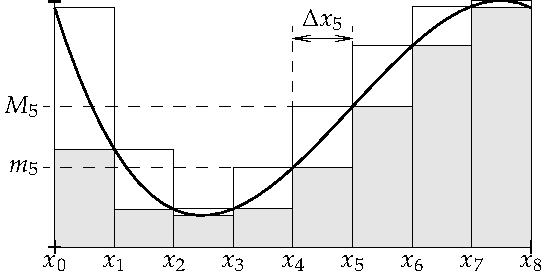
\includegraphics{figures/darbouxfig}
\caption{Sample Darboux sums.\label{darbouxfig}}
\end{myfigureht}

\begin{prop} \label{sumulbound:prop}
Let $f \colon [a,b] \to \R$ be a bounded function.  Let $m, M \in \R$ be 
such that for all $x$ we have $m \leq f(x) \leq M$.  For any partition $P$ of $[a,b]$
we have
\begin{equation}
\label{sumulbound:eq}
m(b-a) \leq
L(P,f) \leq U(P,f)
\leq M(b-a) .
\end{equation}
\end{prop}

\begin{proof}
Let $P$ be a partition.  Then note that $m \leq m_i$ for all $i$ and
$M_i \leq M$ for all $i$.  Also $m_i \leq M_i$ for all $i$.  Finally
$\sum_{i=1}^n \Delta x_i = (b-a)$.  Therefore,
\begin{multline*}
m(b-a) =
m \left( \sum_{i=1}^n \Delta x_i \right)
=
\sum_{i=1}^n m \Delta x_i
\leq
\sum_{i=1}^n m_i \Delta x_i 
\leq
\\
\leq
\sum_{i=1}^n M_i \Delta x_i
\leq
\sum_{i=1}^n M \Delta x_i 
=
M \left( \sum_{i=1}^n \Delta x_i \right)
=
M(b-a) .
\end{multline*}
Hence we get \eqref{sumulbound:eq}.  In particular, the set of lower and
upper sums are bounded sets.
\end{proof}

\begin{defn}
As the sets of lower and upper Darboux sums are bounded, we define
\begin{align*}
& \underline{\int_a^b} f(x)~dx :=
\sup \, \bigl\{ L(P,f) : P \text{ a partition of } [a,b] \bigr\} , \\
& \overline{\int_a^b} f(x)~dx :=
\inf \, \bigl\{ U(P,f) : P \text{ a partition of } [a,b] \bigr\} .
\end{align*}
We call $\underline{\int}$\glsadd{not:lowerdarboux}
the \emph{\myindex{lower Darboux integral}} and
$\overline{\int}$\glsadd{not:upperdarboux} the
\emph{\myindex{upper Darboux integral}}\index{Darboux integral}.
To avoid worrying about the variable of integration, 
we often simply write
\begin{equation*}
\underline{\int_a^b} f :=
\underline{\int_a^b} f(x)~dx 
\qquad \text{and} \qquad
\overline{\int_a^b} f :=
\overline{\int_a^b} f(x)~dx  .
\end{equation*}
\end{defn}

If integration is to make sense, then the lower and upper Darboux
integrals should be the same number, as we want a single number to call
\emph{the integral}.  However, these two integrals may differ for
some functions.

\begin{example} \label{example:dirichletfunc}
Take the \myindex{Dirichlet function}
$f \colon [0,1] \to \R$, where $f(x) := 1$ if
$x \in \Q$ and $f(x) := 0$ if $x \notin \Q$.  Then
\begin{equation*}
\underline{\int_0^1} f = 0 \qquad \text{and} \qquad
\overline{\int_0^1} f = 1 .
\end{equation*}
The reason is that for every $i$ we have 
$m_i = \inf \{ f(x) : x \in [x_{i-1},x_i] \} = 0$  and
$M_i = \sup \{ f(x) : x \in [x_{i-1},x_i] \} = 1$.  Thus
\begin{align*}
& L(P,f) = \sum_{i=1}^n 0 \cdot \Delta x_i = 0 , \\
& U(P,f) = \sum_{i=1}^n 1 \cdot \Delta x_i = \sum_{i=1}^n \Delta x_i = 1  .
\end{align*}
\end{example}

\begin{remark}
The same definition of $\underline{\int_a^b} f$ and
$\overline{\int_a^b} f$
is used when $f$ is defined on a larger set $S$ such that
$[a,b] \subset S$.  In that case, we use the restriction of $f$ to $[a,b]$
and we must ensure that the restriction is bounded on $[a,b]$.
\end{remark}

To compute the integral we often take a partition $P$ and make it finer.
That is, we cut intervals in the partition into yet smaller pieces.

\begin{defn}
Let $P := \{ x_0, x_1, \ldots, x_n \}$ and
$\widetilde{P} := \{ \widetilde{x}_0, \widetilde{x}_1, \ldots, \widetilde{x}_m \}$ be
partitions of $[a,b]$.  We say $\widetilde{P}$ is a
\emph{refinement}\index{refinement of a partition} of $P$
if as sets $P \subset \widetilde{P}$.
\end{defn}

That is, $\widetilde{P}$ is a refinement of a partition if it contains all the
numbers in $P$ and perhaps some other numbers in between.  For example,
$\{ 0, 0.5, 1, 2 \}$ is a partition of $[0,2]$ and
$\{ 0, 0.2, 0.5, 1, 1.5, 1.75, 2 \}$ is a refinement.
The main reason for introducing refinements is the following proposition.

\begin{prop} \label{prop:refinement}
Let $f \colon [a,b] \to \R$ be a bounded function, and let $P$
be a partition of $[a,b]$.  Let $\widetilde{P}$ be a refinement of $P$.
Then
\begin{equation*}
L(P,f) \leq L(\widetilde{P},f) 
\qquad \text{and} \qquad
U(\widetilde{P},f) \leq U(P,f) .
\end{equation*}
\end{prop}

\begin{proof}
The tricky part of this proof is to get the notation correct.
Let $\widetilde{P} := \{ \widetilde{x}_0, \widetilde{x}_1, \ldots,
\widetilde{x}_m \}$ be
a refinement of 
$P := \{ x_0, x_1, \ldots, x_n \}$.  Then
$x_0 = \widetilde{x}_0$ and 
$x_n = \widetilde{x}_m$.  In fact, we can find integers
$k_0 < k_1 < \cdots < k_n$ such that $x_j = \widetilde{x}_{k_j}$ for
$j=0,1,2,\ldots,n$.

Let $\Delta \widetilde{x}_p = \widetilde{x}_p - \widetilde{x}_{p-1}$.
See \figureref{fig:refinement}.
We get 
\begin{equation*}
\Delta x_j
=
x_j - x_{j-1} =
\widetilde{x}_{k_j} - \widetilde{x}_{k_{j-1}} =
\sum_{p=k_{j-1}+1}^{k_j} 
\widetilde{x}_{p} - \widetilde{x}_{p-1}
=
\sum_{p=k_{j-1}+1}^{k_j} \Delta \widetilde{x}_p .
\end{equation*}
\begin{myfigureht}
\subimport*{figures/}{figrefinement.pdf_t}
\caption{Refinement of a subinterval.  Notice $\Delta x_j =
\Delta \widetilde{x}_{p-2} +
\Delta \widetilde{x}_{p-1} +
\Delta \widetilde{x}_{p}$,
and also
$k_{j-1}+1 = p-2$ and
$k_{j} = p$.\label{fig:refinement}}
\end{myfigureht}

Let $m_j$ be as before and correspond to the partition $P$.
Let $\widetilde{m}_j := \inf \{ f(x) : \widetilde{x}_{j-1} \leq x \leq
\widetilde{x}_j \}$.
Now, $m_j \leq \widetilde{m}_p$ for $k_{j-1} < p \leq k_j$.  Therefore,
\begin{equation*}
m_j \Delta x_j
=
m_j \sum_{p=k_{j-1}+1}^{k_j} \Delta \widetilde{x}_p
=
\sum_{p=k_{j-1}+1}^{k_j} m_j \Delta \widetilde{x}_p
\leq
\sum_{p=k_{j-1}+1}^{k_j} \widetilde{m}_p \Delta \widetilde{x}_p .
\end{equation*}
So
\begin{equation*}
L(P,f) =
\sum_{j=1}^n m_j \Delta x_j
\leq
\sum_{j=1}^n \,
\sum_{p=k_{j-1}+1}^{k_j} \widetilde{m}_p \Delta \widetilde{x}_p
=
\sum_{j=1}^m
\widetilde{m}_j \Delta \widetilde{x}_j = L(\widetilde{P},f).
\end{equation*}

The proof of $U(\widetilde{P},f) \leq U(P,f)$ is left as an exercise.
\end{proof}

Armed with refinements we prove the following.
The key point of this next proposition is that
the lower Darboux integral is less than or equal to the upper Darboux
integral.

\begin{prop} \label{intulbound:prop}
Let $f \colon [a,b] \to \R$ be a bounded function.  Let $m, M \in \R$ be 
such that for all $x \in [a,b]$ we have $m \leq f(x) \leq M$.  Then
\begin{equation}
\label{intulbound:eq}
m(b-a) \leq
\underline{\int_a^b} f \leq \overline{\int_a^b} f
\leq M(b-a) .
\end{equation}
\end{prop}

\begin{proof}
By \propref{sumulbound:prop} we have for any partition $P$
\begin{equation*}
m(b-a) \leq L(P,f) \leq U(P,f) \leq M(b-a).
\end{equation*}
The inequality
$m(b-a) \leq L(P,f)$ implies $m(b-a) \leq \underline{\int_a^b} f$.
Also
$U(P,f) \leq M(b-a)$ implies $\overline{\int_a^b} f \leq M(b-a)$.

The middle inequality in
\eqref{intulbound:eq} is the main point of this proposition.
Let $P_1, P_2$ be partitions of $[a,b]$.  Define 
$\widetilde{P} := P_1 \cup P_2$.
The set $\widetilde{P}$ is a partition of $[a,b]$, which
is a refinement of $P_1$ and a refinement of $P_2$.
By \propref{prop:refinement},
$L(P_1,f) \leq L(\widetilde{P},f)$ and
$U(\widetilde{P},f) \leq U(P_2,f)$.  So
\begin{equation*}
L(P_1,f) \leq L(\widetilde{P},f) \leq U(\widetilde{P},f) \leq U(P_2,f) .
\end{equation*}
In other words, for two arbitrary partitions $P_1$ and $P_2$, we have
$L(P_1,f) \leq U(P_2,f)$.  
Recall \propref{infsupineq:prop}, and take the supremum and
infimum over all partitions:
\begin{equation*}
\underline{\int_a^b} f = 
\sup \, \bigl\{ L(P,f) : P \text{ a partition of } [a,b] \bigr\}
\leq
\inf \, \bigl\{ U(P,f) : P \text{ a partition of } [a,b] \bigr\}
=
\overline{\int_a^b} f . \qedhere
\end{equation*}
\end{proof}

\subsection{Riemann integral}

We can finally define the Riemann integral.  However, the Riemann
integral is only defined on a certain class of functions, called the
Riemann integrable functions.

\begin{defn}
Let $f \colon [a,b] \to \R$ be a bounded function such that
\begin{equation*}
\underline{\int_a^b} f(x)~dx = \overline{\int_a^b} f(x)~dx .
\end{equation*}
Then $f$ is said to be \emph{\myindex{Riemann integrable}}.
The set of Riemann integrable functions on $[a,b]$ is denoted
by $\sR[a,b]$.\glsadd{not:integrablefunc}
When $f \in \sR[a,b]$ we define\glsadd{not:riemannint}
\begin{equation*}
\int_a^b f(x)~dx := 
\underline{\int_a^b} f(x)~dx = \overline{\int_a^b} f(x)~dx .
\end{equation*}
As before, we often simply write
\begin{equation*}
\int_a^b f := \int_a^b f(x)~dx.
\end{equation*}
The number $\int_a^b f$ is called the \emph{\myindex{Riemann integral}}
of $f$, or sometimes simply the \emph{integral} of $f$.
\end{defn}

By definition, any Riemann integrable function is bounded.
By appealing to \propref{intulbound:prop} we immediately obtain
the following proposition.  See also \figureref{fig:integralminmax}.

\begin{prop} \label{intbound:prop}
Let $f \colon [a,b] \to \R$ be a Riemann integrable function.
Let $m, M \in \R$ be 
such that $m \leq f(x) \leq M$ for all $x \in [a,b]$.  Then
\begin{equation*}
m(b-a) \leq
\int_a^b f
\leq M(b-a) .
\end{equation*}
\end{prop}
\begin{myfigureht}
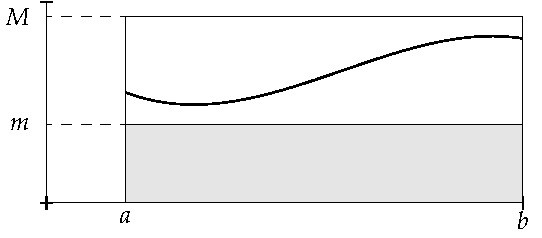
\includegraphics{figures/integralminmax}
\caption{The area under the curve is bounded from above by
the area of the entire rectangle, $M(b-a)$, and from below by
the area of the shaded part, $m(b-a)$.\label{fig:integralminmax}}
\end{myfigureht}

Often we use a weaker form of this proposition.  That is, if
$\abs{f(x)} \leq M$ for all $x \in [a,b]$, then
\begin{equation*}
\abs{\int_a^b f} \leq M(b-a) .
\end{equation*}

\begin{example}
We integrate constant functions using
\propref{intulbound:prop}.
If $f(x) := c$ for some constant $c$, then we take $m = M = c$.
In inequality \eqref{intulbound:eq}
all the inequalities must be equalities.
Thus $f$ is integrable on $[a,b]$ and $\int_a^b f = c(b-a)$.
\end{example}

\begin{example}
Let $f \colon [0,2] \to \R$ be defined by
\begin{equation*}
f(x) :=
\begin{cases}
1               & \text{if } x < 1,\\
\nicefrac{1}{2} & \text{if } x = 1,\\
0               & \text{if } x > 1.
\end{cases}
\end{equation*}
We claim $f$ is Riemann integrable and $\int_0^2 f = 1$.

Proof: Let $0 < \epsilon < 1$ be arbitrary.
Let $P := \{0, 1-\epsilon, 1+\epsilon, 2\}$ be a partition.  We use the notation from
the definition of the Darboux sums.  Then
\begin{align*}
m_1 &= \inf \, \bigl\{ f(x) : x \in [0,1-\epsilon] \bigr\} = 1 , & 
M_1 &= \sup \, \bigl\{ f(x) : x \in [0,1-\epsilon] \bigr\} = 1 , \\
m_2 &= \inf \, \bigl\{ f(x) : x \in [1-\epsilon,1+\epsilon] \bigr\} = 0 , & 
M_2 &= \sup \, \bigl\{ f(x) : x \in [1-\epsilon,1+\epsilon] \bigr\} = 1 , \\
m_3 &= \inf \, \bigl\{ f(x) : x \in [1+\epsilon,2] \bigr\} = 0 , & 
M_3 &= \sup \, \bigl\{ f(x) : x \in [1+\epsilon,2] \bigr\} = 0 .
\end{align*}
Furthermore, $\Delta x_1 = 1-\epsilon$, $\Delta x_2 = 2\epsilon$ and
$\Delta x_3 = 1-\epsilon$.
See \figureref{darbouxfigstep}.
\begin{myfigureht}
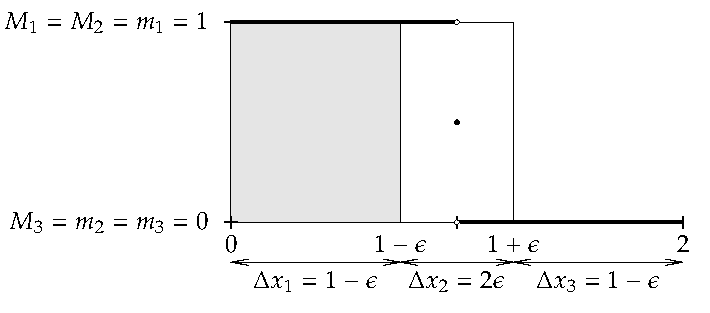
\includegraphics{figures/darbouxfigstep}
\caption{Darboux sums for the step function.  $L(P,f)$ is the area of the
shaded rectangle, $U(P,f)$ is the area of both rectangles, and
$U(P,f)-L(P,f)$ is the area of the unshaded rectangle.\label{darbouxfigstep}}
\end{myfigureht}

We compute
\begin{align*}
& L(P,f) = \sum_{i=1}^3 m_i \Delta x_i =
1 \cdot (1-\epsilon) + 0 \cdot 2\epsilon + 0 \cdot (1-\epsilon)
= 1-\epsilon , \\
& U(P,f) = \sum_{i=1}^3 M_i \Delta x_i =
1 \cdot (1-\epsilon) + 1 \cdot 2\epsilon + 0 \cdot (1-\epsilon)
= 1+\epsilon .
\end{align*}
Thus,
\begin{equation*}
\overline{\int_0^2} f - 
\underline{\int_0^2} f
\leq
U(P,f) - L(P,f)
=
(1+\epsilon)
- (1-\epsilon) = 2 \epsilon .
\end{equation*}
By \propref{intulbound:prop} we have $\underline{\int_0^2} f \leq \overline{\int_0^2} f$.
As $\epsilon$ was arbitrary we see 
$\overline{\int_0^2} f = \underline{\int_0^2} f$.  So $f$ is Riemann
integrable.  Finally,
\begin{equation*}
1-\epsilon = L(P,f) \leq \int_0^2 f \leq U(P,f) =
1+\epsilon.
\end{equation*}
Hence, $\bigl\lvert \int_0^2 f - 1 \bigr\rvert \leq \epsilon$.  As $\epsilon$ was arbitrary,
we have $\int_0^2 f = 1$.
\end{example}

It may be worthwhile to extract part of the technique of the example into a
proposition.

\begin{prop}
Let $f \colon [a,b] \to \R$ be a bounded function.  Then $f$ is Riemann
integrable if for every $\epsilon > 0$, there exists a partition $P$ such that
\begin{equation*}
U(P,f) - L(P,f) < \epsilon .
\end{equation*}
\end{prop}

\begin{proof}
If for every $\epsilon > 0$ such a $P$ exists, then we have:
\begin{equation*}
0 \leq
\overline{\int_a^b} f - 
\underline{\int_a^b} f
\leq
U(P,f) - L(P,f) < \epsilon .
\end{equation*}
Therefore, 
$\overline{\int_a^b} f = \underline{\int_a^b} f$, and $f$ is integrable.
\end{proof}

\begin{example}
Let us show $\frac{1}{1+x}$ is integrable on $[0,b]$ for any $b > 0$.
We will see later that all continuous functions are integrable, but let us
demonstrate how we do it directly.

Let $\epsilon > 0$ be given.  Take $n \in \N$ and
pick $x_j := \nicefrac{jb}{n}$, to form the 
partition $P := \{ x_0,x_1,\ldots,x_n \}$ of $[0,b]$.
We have $\Delta x_j = \nicefrac{b}{n}$ for all $j$.  
As $f$ is decreasing, for any subinterval $[x_{j-1},x_j]$ we obtain
\begin{equation*}
m_j = \inf \left\{ \frac{1}{1+x} : x \in [x_{j-1},x_j] \right\} = \frac{1}{1+x_j} ,
\qquad
M_j = \sup \left\{ \frac{1}{1+x} : x \in [x_{j-1},x_j] \right\} =
\frac{1}{1+x_{j-1}} .
\end{equation*}
Then we have
\begin{multline*}
U(P,f)-L(P,f)
=
\sum_{j=1}^n
\Delta x_j
(M_j-m_j)
=
\frac{b}{n}
\sum_{j=1}^n 
\left( \frac{1}{1+\nicefrac{(j-1)b}{n}} - \frac{1}{1+\nicefrac{jb}{n}} \right) 
=
\\
=
\frac{b}{n}
\left( \frac{1}{1+\nicefrac{0b}{n}} - \frac{1}{1+\nicefrac{nb}{n}} \right) 
=
\frac{b^2}{n(b+1)} .
\end{multline*}
The sum telescopes, the terms successively cancel each other, something
we have seen before.
Picking $n$ to be such that
$\frac{b^2}{n(b+1)} < \epsilon$ the proposition is satisfied, and the
function is integrable.
\end{example}

\begin{remark}
A way of thinking of the integral is that it adds up (integrates) lots of
local information---it sums $f(x)~dx$ over all $x$.
The integral sign was chosen by Leibniz to be the long S, to mean summation.
Unlike derivatives, which are \myquote{local,} 
integrals show up in applications when
one wants a \myquote{global} answer: total distance travelled, average
temperature, total charge, etc.
\end{remark}

\subsection{More notation}

When $f \colon S \to \R$ is defined on a larger set $S$ and
$[a,b] \subset S$,
we say $f$ is Riemann integrable on $[a,b]$ if the restriction of $f$
to $[a,b]$ is Riemann integrable. 
In this case,
we say $f \in \sR[a,b]$,
and
we write $\int_a^b f$ to mean the Riemann integral
of the restriction of $f$ to $[a,b]$.

It is useful to define the integral $\int_a^b f$ even if
$a \not< b$.  Suppose $b < a$ and $f \in \sR[b,a]$,
then define
\begin{equation*}
\int_a^b f := - \int_b^a f .
\end{equation*}
For any function $f$, define
\begin{equation*}
\int_a^a f := 0 .
\end{equation*}

At times, the variable $x$ may already have some other meaning.  When
we need to write down the variable of integration, we may simply
use a different letter.  For example,
\begin{equation*}
\int_a^b f(s)~ds := \int_a^b f(x)~dx .
\end{equation*}

\subsection{Exercises}

\begin{exercise}
Define $f \colon [0,1] \to \R$ by $f(x) := x^3$
and let $P := \{ 0, 0.1, 0.4, 1 \}$.  Compute $L(P,f)$ and $U(P,f)$.
\end{exercise}

\begin{exercise}
Let $f \colon [0,1] \to \R$ be defined by $f(x) := x$.
Show that $f \in \sR[0,1]$ and
compute $\int_0^1 f$ using the definition of the integral
(but
feel free to use the propositions of this section).%\propref{intulbound:prop}).
\end{exercise}

\begin{exercise}
Let $f \colon [a,b] \to \R$ be a bounded function.
Suppose there exists a sequence of partitions $\{ P_k \}$ of $[a,b]$
such that
\begin{equation*}
\lim_{k \to \infty} \bigl( U(P_k,f) - L(P_k,f) \bigr) = 0 .
\end{equation*}
Show that $f$ is Riemann integrable and that
\begin{equation*}
\int_a^b f = 
\lim_{k \to \infty} U(P_k,f)
=
\lim_{k \to \infty} L(P_k,f) .
\end{equation*}
\end{exercise}

\begin{exercise}
Finish the proof of \propref{prop:refinement}.
\end{exercise}

\begin{exercise}
Suppose $f \colon [-1,1] \to \R$ is defined as
\begin{equation*}
f(x) :=
\begin{cases}
1 & \text{if } x > 0, \\
0 & \text{if } x \leq 0.
\end{cases}
\end{equation*}
Prove that $f \in \sR[-1,1]$ and
compute $\int_{-1}^1 f$ using the definition of the integral
(but
feel free to use the propositions of this section).
%(feel free to use \propref{intulbound:prop}).
\end{exercise}

\begin{exercise}
Let $c \in (a,b)$ and let $d \in \R$.
Define $f \colon [a,b] \to \R$ as
\begin{equation*}
f(x) :=
\begin{cases}
d & \text{if } x = c, \\
0 & \text{if } x \not= c.
\end{cases}
\end{equation*}
Prove that $f \in \sR[a,b]$ and
compute
$\int_a^b f$ using the definition of the integral
%(feel free to use \propref{intulbound:prop}).
(but
feel free to use the propositions of this section).
\end{exercise}

\begin{exercise} \label{exercise:taggedpartition}
Suppose $f \colon [a,b] \to \R$ is Riemann integrable.  Let $\epsilon
> 0$ be given.  Then show that there exists a partition $P = \{ x_0, x_1,
\ldots, x_n \}$
such that if we
pick any set of numbers $\{ c_1, c_2, \ldots, c_n \}$ with
$c_k \in [x_{k-1},x_k]$ for all $k$, then
\begin{equation*}
\abs{\int_a^b f - \sum_{k=1}^n f(c_k) \Delta x_k} < \epsilon .
\end{equation*}
\end{exercise}

\begin{exercise}
Let $f \colon [a,b] \to \R$ be a Riemann integrable function.
Let $\alpha > 0$ and $\beta \in \R$.
Then define $g(x) := f(\alpha x + \beta)$ on the interval
$I = [\frac{a-\beta}{\alpha}, \frac{b-\beta}{\alpha}]$.  Show
that $g$ is Riemann integrable on $I$.
\end{exercise}

\begin{exercise}
Suppose $f \colon [0,1] \to \R$ and $g \colon [0,1] \to \R$
are such that for all $x \in (0,1]$
we have $f(x) = g(x)$.  Suppose $f$ is Riemann integrable. 
Prove $g$ is Riemann integrable and $\int_{0}^1 f = \int_{0}^1 g$.
\end{exercise}

\begin{exercise}
Let $f \colon [0,1] \to \R$ be a bounded function.
Let $P_n = \{ x_0,x_1,\ldots,x_n \}$ be a uniform partition of $[0,1]$,
that is, $x_j := \nicefrac{j}{n}$.  Is $\{ L(P_n,f) \}_{n=1}^\infty$
always monotone?  Yes/No: Prove or find a counterexample.
\end{exercise}

\begin{exercise}[Challenging]
For a bounded function $f \colon [0,1] \to \R$ let
$R_n := (\nicefrac{1}{n})\sum_{j=1}^n f(\nicefrac{j}{n})$ (the
uniform right hand rule).
\begin{enumerate}[a)]
\item
If $f$ is Riemann integrable show $\int_0^1 f = \lim \, R_n$.
\item
Find an $f$ that is not Riemann integrable, but $\lim \, R_n$ exists.
\end{enumerate}
\end{exercise}

\begin{exercise}[Challenging] \label{exercise:riemannintdarboux}
Generalize the previous exercise.
Show that $f \in \sR[a,b]$ if and only if there exists an $I \in \R$,
such that for every $\epsilon > 0$ there exists
a $\delta > 0$ such that if $P$ is a partition with $\Delta x_i < \delta$
for all $i$, then
$\abs{L(P,f) - I} < \epsilon$ and
$\abs{U(P,f) - I} < \epsilon$.  If $f \in \sR[a,b]$, then $I = \int_a^b f$.
\end{exercise}

\begin{exercise}
Using \exerciseref{exercise:riemannintdarboux} and the idea of
the proof in \exerciseref{exercise:taggedpartition}, show that 
Darboux integral is the same as the standard definition
of Riemann integral, which you have most likely seen in calculus.  That is,
show that
$f \in \sR[a,b]$ if and only if there exists an $I \in \R$,
such that for every $\epsilon > 0$ there exists
a $\delta > 0$ such that if $P = \{ x_0,x_1,\ldots,x_n \}$
is a partition with $\Delta x_i < \delta$
for all $i$, then
$\abs{\sum_{i=1}^n f(c_i) \Delta x_i - I} < \epsilon$ for any set
$\{ c_1,c_2,\ldots,c_n \}$ with $c_i \in [x_{i-1},x_i]$.
If $f \in \sR[a,b]$, then $I = \int_a^b f$.
\end{exercise}


\begin{exercise}[Challenging]
Construct functions $f$ and $g$, 
where
$f \colon [0,1] \to \R$ is Riemann integrable,
$g \colon [0,1] \to [0,1]$ is one-to-one and onto,
and such that the composition $f \circ g$ is not Riemann integrable.
\end{exercise}

%%%%%%%%%%%%%%%%%%%%%%%%%%%%%%%%%%%%%%%%%%%%%%%%%%%%%%%%%%%%%%%%%%%%%%%%%%%%%%

\sectionnewpage
\section{Properties of the integral}
\label{sec:rintprop}

\sectionnotes{2 lectures, integrability of functions with 
discontinuities can safely be skipped}

\subsection{Additivity}

Adding a bunch of things in two parts and then adding those two parts
should be the same as adding everything all at once.
The corresponding property for integral is called the
\myindex{additive property of the integral}.  First, we prove the additivity
property for the lower and upper Darboux integrals.

\begin{lemma} \label{lemma:darbouxadd}
Suppose $a < b < c$ and $f \colon [a,c] \to \R$ is a bounded function.
Then
\begin{equation*}
\underline{\int_a^c} f
=
\underline{\int_a^b} f
+
\underline{\int_b^c} f
\end{equation*}
and
\begin{equation*}
\overline{\int_a^c} f
=
\overline{\int_a^b} f
+
\overline{\int_b^c} f .
\end{equation*}
\end{lemma}

\begin{proof}
If we have partitions $P_1 = \{ x_0,x_1,\ldots,x_k \}$
of $[a,b]$ and $P_2 = \{ x_k, x_{k+1}, \ldots, x_n \}$ of $[b,c]$,
then the set $P := P_1 \cup P_2 = \{ x_0, x_1, \ldots, x_n \}$ is
a partition of $[a,c]$.  Then
\begin{equation*}
L(P,f) =
\sum_{j=1}^n m_j \Delta x_j
=
\sum_{j=1}^k m_j \Delta x_j
+
\sum_{j=k+1}^n m_j \Delta x_j
=
L(P_1,f) + L(P_2,f) .
\end{equation*}
When we take the supremum of the right hand side over all $P_1$ and $P_2$,
we are taking a supremum of the left hand side
over all partitions $P$ of $[a,c]$ that contain $b$.  If $Q$ is any partition
of $[a,c]$ and $P = Q \cup \{ b \}$, then $P$ is a refinement of $Q$
and so $L(Q,f) \leq L(P,f)$.  Therefore, taking a supremum only over the $P$
that contain $b$ is sufficient to find the supremum of $L(P,f)$
over all partitions $P$, see \exerciseref{exercise:dominatingb}.
Finally recall \exerciseref{exercise:supofsum}
to compute
\begin{equation*}
\begin{split}
\underline{\int_a^c} f
& =
\sup \, \bigl\{ L(P,f) : P \text{ a partition of } [a,c] \bigr\}
\\
& =
\sup \, \bigl\{ L(P,f) : P \text{ a partition of } [a,c], b \in P \bigr\}
\\
& =
\sup \, \bigl\{ L(P_1,f) + L(P_2,f) :
P_1 \text{ a partition of } [a,b], P_2 \text{ a partition of } [b,c] \bigr\}
\\
& =
\sup \, \bigl\{ L(P_1,f) : P_1 \text{ a partition of } [a,b] \bigr\}
+
\sup \, \bigl\{ L(P_2,f) : P_2 \text{ a partition of } [b,c] \bigr\}
\\
&=
\underline{\int_a^b} f + \underline{\int_b^c} f .
\end{split}
\end{equation*}

Similarly, for $P$, $P_1$, and $P_2$ as above we obtain
\begin{equation*}
U(P,f) =
\sum_{j=1}^n M_j \Delta x_j
=
\sum_{j=1}^k M_j \Delta x_j
+
\sum_{j=k+1}^n M_j \Delta x_j
=
U(P_1,f) + U(P_2,f) .
\end{equation*}
We wish to take the infimum on the right
over all $P_1$ and $P_2$, and so we are taking the infimum
over all partitions $P$ of $[a,c]$ that contain $b$.  If $Q$ is any partition
of $[a,c]$ and $P = Q \cup \{ b \}$, then $P$ is a refinement of $Q$
and so $U(Q,f) \geq U(P,f)$.  Therefore, taking an infimum only over the $P$
that contain $b$ is sufficient to find the infimum of $U(P,f)$ for
all $P$.
We obtain
\begin{equation*}
\overline{\int_a^c} f
=
\overline{\int_a^b} f + \overline{\int_b^c} f .  \qedhere
\end{equation*}
\end{proof}

\begin{prop}
Let $a < b < c$.  A function $f \colon [a,c] \to \R$ is Riemann integrable
if and only if $f$ is Riemann integrable on $[a,b]$ and $[b,c]$.  If
$f$ is Riemann integrable, then
\begin{equation*}
\int_a^c f
=
\int_a^b f
+
\int_b^c f .
\end{equation*}
\end{prop}

\begin{proof}
Suppose $f \in \sR[a,c]$, then 
$\overline{\int_a^c} f = 
\underline{\int_a^c} f = 
\int_a^c f$.  We apply the lemma to get
\begin{equation*}
\int_a^c f
=
\underline{\int_a^c} f
 =
\underline{\int_a^b} f + \underline{\int_b^c} f
 \leq
\overline{\int_a^b} f + \overline{\int_b^c} f
 =
\overline{\int_a^c} f
 =
\int_a^c f .
\end{equation*}
Thus the inequality is an equality,
\begin{equation*}
\underline{\int_a^b} f + \underline{\int_b^c} f
=
\overline{\int_a^b} f + \overline{\int_b^c} f .
\end{equation*}
As we also know 
$\underline{\int_a^b} f \leq \overline{\int_a^b} f$
and
$\underline{\int_b^c} f \leq \overline{\int_b^c} f$, we 
conclude 
\begin{equation*}
\underline{\int_a^b} f
=
\overline{\int_a^b} f
\qquad \text{and} \qquad
\underline{\int_b^c} f
=
\overline{\int_b^c} f .
\end{equation*}
Thus $f$ is Riemann integrable on $[a,b]$ and $[b,c]$ and the desired formula
holds.

Now assume $f$ is Riemann integrable on $[a,b]$ and on $[b,c]$.
Again apply the lemma to get
\begin{equation*}
\underline{\int_a^c} f
=
\underline{\int_a^b} f + \underline{\int_b^c} f
=
\int_a^b f + \int_b^c f
=
\overline{\int_a^b} f + \overline{\int_b^c} f
=
\overline{\int_a^c} f .
\end{equation*}
Therefore, $f$ is Riemann integrable on $[a,c]$, and the integral is computed
as indicated.
\end{proof}

An easy consequence of the additivity is the following corollary.  We
leave the details to the reader as an exercise.

\begin{cor} \label{intsubcor}
If $f \in \sR[a,b]$ and
$[c,d] \subset [a,b]$, then
the restriction $f|_{[c,d]}$ is in $\sR[c,d]$.
\end{cor}

\subsection{Linearity and monotonicity}

A sum is a linear function of the summands.  So is the integral.

\begin{prop}[Linearity]
\index{linearity of the integral}\label{prop:integrallinear}
Let $f$ and $g$ be in $\sR[a,b]$ and $\alpha \in \R$.
\begin{enumerate}[(i)]
\item $\alpha f$ is in $\sR[a,b]$ and
\begin{equation*}
\int_a^b \alpha f(x) ~dx = \alpha \int_a^b f(x) ~dx .
\end{equation*}
\item $f+g$ is in $\sR[a,b]$ and
\begin{equation*}
\int_a^b \bigl( f(x)+g(x) \bigr) ~dx = 
\int_a^b f(x) ~dx 
+
\int_a^b g(x) ~dx .
\end{equation*}
\end{enumerate}
\end{prop}

\pagebreak[2]
\begin{proof}
Let us prove the first item for $\alpha \geq 0$. 
Let $P$ be a partition of $[a,b]$.
Let $m_i := \inf \{ f(x) : x \in [x_{i-1},x_i] \}$ as usual.
Since $\alpha$ is nonnegative, we can move the multiplication by $\alpha$
past the infimum,
\begin{equation*}
\inf \{ \alpha f(x) : x \in [x_{i-1},x_i] \}
=
\alpha \inf \{ f(x) : x \in [x_{i-1},x_i] \} = \alpha m_i .
\end{equation*}
Therefore,
\begin{equation*}
L(P,\alpha f) =
\sum_{i=1}^n \alpha m_i \Delta x_i = \alpha \sum_{i=1}^n m_i \Delta x_i = \alpha
L(P,f).
\end{equation*}
Similarly,
\begin{equation*}
U(P,\alpha f) = \alpha U(P,f) .
\end{equation*}
Again, as $\alpha \geq 0$ we
may move multiplication by $\alpha$ past the supremum.  Hence,
\begin{equation*}
\begin{split}
\underline{\int_a^b} \alpha f(x)~dx & =
\sup \, \bigl\{ L(P,\alpha f) : P \text{ a partition of } [a,b] \bigr\}
\\
& =
\sup \, \bigl\{ \alpha L(P,f) : P \text{ a partition of } [a,b] \bigr\}
\\
& =
\alpha \,
\sup \, \bigl\{ L(P,f) : P \text{ a partition of } [a,b] \bigr\}
\\
& =
\alpha
\underline{\int_a^b} f(x)~dx .
\end{split}
\end{equation*}
Similarly, we show 
\begin{equation*}
\overline{\int_a^b} \alpha f(x)~dx
=
\alpha
\overline{\int_a^b} f(x)~dx .
\end{equation*}
The conclusion now follows for $\alpha \geq 0$.

To finish the proof of the first item, we need to show 
that $-f$ is Riemann integrable and
$\int_a^b - f(x)~dx =
-
\int_a^b f(x)~dx$.  The proof of this fact is left as
\exerciseref{exercise:proofoflinpropparti}.

The proof of the second item in the proposition is also left as
\exerciseref{exercise:proofoflinproppartii}.
It is not as
trivial as it may appear at first glance.
\end{proof}

The second item in the proposition does not hold with
equality for the Darboux integrals, but we do obtain inequalities.
The proof of the following proposition is \exerciseref{exercise:upperlowerlinineq}.
It follows for upper and lower sums on a fixed partition by \exerciseref{exercise:sumofsup},
that is, supremum of a sum is less than or equal to the sum of
suprema and similarly for infima.

\begin{prop} \label{prop:upperlowerlinineq}
Let $f \colon [a,b] \to \R$ and $g \colon [a,b] \to \R$ be bounded
functions.  Then
\begin{equation*}
%\overline{\int_a^b} \bigl(f(x)+g(x)\bigr)~dx \leq
%\overline{\int_a^b}f(x)~dx+\overline{\int_a^b}g(x)~dx
\overline{\int_a^b} (f+g) \leq \overline{\int_a^b}f+\overline{\int_a^b}g
,
\qquad
\text{and}
\qquad
\underline{\int_a^b} (f+g) \geq \underline{\int_a^b}f+\underline{\int_a^b}g
%\underline{\int_a^b} \bigl(f(x)+g(x)\bigr)~dx \geq
%\underline{\int_a^b}f(x)~dx+\underline{\int_a^b}g(x)~dx
.
\end{equation*}
\end{prop}

Adding up smaller numbers should give us a smaller result.
That is true for an integral as well.

\begin{prop}[Monotonicity]
\index{monotonicity of the integral}
Let $f \colon [a,b] \to \R$ and $g \colon [a,b] \to \R$ be
bounded, and $f(x) \leq g(x)$
for all $x \in [a,b]$.  Then
\begin{equation*}
\underline{\int_a^b} f 
\leq
\underline{\int_a^b} g 
\qquad \text{and} \qquad
\overline{\int_a^b} f 
\leq
\overline{\int_a^b} g .
\end{equation*}
Moreover, if $f$ and $g$ are in $\sR[a,b]$, then
\begin{equation*}
\int_a^b f 
\leq
\int_a^b g .
\end{equation*}
\end{prop}

\begin{proof}
Let $P = \{ x_0, x_1, \ldots, x_n \}$ be a partition of $[a,b]$.  Then
let
\begin{equation*}
m_i := \inf \, \bigl\{ f(x) : x \in [x_{i-1},x_i] \bigr\}
\qquad \text{and} \qquad
\widetilde{m}_i := \inf \, \bigl\{ g(x) : x \in [x_{i-1},x_i] \bigr\} .
\end{equation*}
As $f(x) \leq g(x)$, then $m_i \leq \widetilde{m}_i$.
Therefore,
\begin{equation*}
L(P,f)
=
\sum_{i=1}^n m_i \Delta x_i
\leq
\sum_{i=1}^n \widetilde{m}_i \Delta x_i
=
L(P,g) .
\end{equation*}
We take the supremum over all $P$ (see \propref{prop:funcsupinf}) to obtain 
\begin{equation*}
\underline{\int_a^b} f 
\leq
\underline{\int_a^b} g .
\end{equation*}
Similarly, we obtain the same conclusion for the upper integrals.
Finally,
if $f$ and $g$ are Riemann integrable all the integrals are equal,
and the conclusion follows.
\end{proof}

\subsection{Continuous functions}

Let us show that continuous functions are Riemann integrable.  In fact, we
will show we can even allow some discontinuities.  We start with a
function continuous on the whole closed interval $[a,b]$.

\begin{lemma} \label{lemma:contint}
If $f \colon [a,b] \to \R$ is a continuous function,
then $f \in \sR[a,b]$.
\end{lemma}

\begin{proof}
As $f$ is continuous on a closed bounded interval, it is
uniformly continuous.
Let $\epsilon > 0$ be given.  Find a $\delta > 0$ such that
$\abs{x-y} < \delta$ implies $\abs{f(x)-f(y)} < \frac{\epsilon}{b-a}$.

Let $P = \{ x_0, x_1, \ldots, x_n \}$
be a partition of $[a,b]$ such that $\Delta x_i < \delta$ for all $i = 1,2,
\ldots, n$.  For example,
take $n$ such that $\frac{b-a}{n} < \delta$ and
let $x_i := \frac{i}{n}(b-a) + a$.
Then for all $x, y \in [x_{i-1},x_i]$ we have 
$\abs{x-y} \leq \Delta x_i < \delta$ and so
\begin{equation*}
f(x)-f(y) \leq \abs{f(x)-f(y)} < \frac{\epsilon}{b-a} .
\end{equation*}
As $f$ is continuous on $[x_{i-1},x_i]$, it attains a maximum and a minimum
on this interval.
Let $x$ be a point where $f$ attains the maximum and $y$ be a point
where $f$ attains the minimum.  Then $f(x) = M_i$
and $f(y) = m_i$ in the notation from the definition of the integral.
Therefore,
\begin{equation*}
M_i-m_i = f(x)-f(y) < 
\frac{\epsilon}{b-a} .
\end{equation*}
And so
\begin{equation*}
\begin{split}
\overline{\int_a^b} f - 
\underline{\int_a^b} f 
& \leq
U(P,f) - L(P,f)
\\
& =
\left(
\sum_{i=1}^n
M_i \Delta x_i
\right)
-
\left(
\sum_{i=1}^n
m_i \Delta x_i
\right)
\\
& =
\sum_{i=1}^n
(M_i-m_i) \Delta x_i
\\
& <
\frac{\epsilon}{b-a}
\sum_{i=1}^n
\Delta x_i
\\
& =
\frac{\epsilon}{b-a} (b-a)
= \epsilon .
\end{split}
\end{equation*}
As $\epsilon > 0$ was arbitrary,
\begin{equation*}
\overline{\int_a^b} f = \underline{\int_a^b} f ,
\end{equation*}
and $f$ is Riemann integrable on $[a,b]$.
\end{proof}

The second lemma says that we need the function to only be \myquote{Riemann integrable
inside the interval,} as long as it is bounded.  It also tells us how to
compute the integral.

\begin{lemma} \label{lemma:boundedimpriemann}
Let $f \colon [a,b] \to \R$ be a bounded function,
$\{ a_n \}$ and $\{b_n \}$ be sequences such that
$a < a_n < b_n < b$ for all $n$, with
$\lim \, a_n = a$ and $\lim \, b_n = b$.
Suppose $f \in \sR[a_n,b_n]$ for all $n$.
Then $f \in \sR[a,b]$ and
\begin{equation*}
\int_a^b f = 
\lim_{n \to \infty} \int_{a_n}^{b_n} f .
\end{equation*}
\end{lemma}

\begin{proof}
Let $M > 0$ be a real number such that $\abs{f(x)} \leq M$.
As $(b-a) \geq (b_n-a_n)$,
\begin{equation*}
-M(b-a) \leq
-M(b_n-a_n) \leq
\int_{a_n}^{b_n} f
\leq
M(b_n-a_n) \leq
M(b-a) .
\end{equation*}
Therefore, the sequence of numbers
$\bigl\{ \int_{a_n}^{b_n} f \bigr\}_{n=1}^\infty$ is bounded and by
\hyperref[thm:bwseq]{Bolzano--Weierstrass}
has a convergent subsequence indexed by $n_k$.  Let us call
$L$ the limit of the subsequence
$\bigl\{ \int_{a_{n_k}}^{b_{n_k}} f \bigr\}_{k=1}^\infty$.

\lemmaref{lemma:darbouxadd} says that
the lower and upper integral are additive
and the hypothesis says that
$f$ is integrable on $[a_{n_k},b_{n_k}]$.
Therefore
\begin{equation*}
\underline{\int_a^b} f
=
\underline{\int_a^{a_{n_k}}} f
+
\int_{a_{n_k}}^{b_{n_k}} f
+
\underline{\int_{b_{n_k}}^b} f
\geq
-M(a_{n_k}-a)
+
\int_{a_{n_k}}^{b_{n_k}} f
-
M(b-b_{n_k}) .
\end{equation*}
We take the limit as $k$ goes to $\infty$ on the right-hand side,
\begin{equation*}
\underline{\int_a^b} f
\geq
-M\cdot 0
+
L
-
M\cdot 0
= L .
\end{equation*}

Next we use additivity of the upper integral,
\begin{equation*}
\overline{\int_a^b} f
=
\overline{\int_a^{a_{n_k}}} f
+
\int_{a_{n_k}}^{b_{n_k}} f
+
\overline{\int_{b_{n_k}}^b} f
\leq
M(a_{n_k}-a)
+
\int_{a_{n_k}}^{b_{n_k}} f
+
M(b-b_{n_k}) .
\end{equation*}
We take the same subsequence 
$\{ \int_{a_{n_k}}^{b_{n_k}} f \}_{k=1}^\infty$ and take the limit 
to obtain
\begin{equation*}
\overline{\int_a^b} f
\leq
M\cdot 0
+
L
+
M\cdot 0
= L .
\end{equation*}
Thus $\overline{\int_a^b} f = \underline{\int_a^b} f = L$
and hence $f$ is Riemann integrable and $\int_a^b f = L$.
In particular, no matter what
subsequence we chose,
the $L$ is the same number.

To prove the final statement of the lemma we use 
\propref{seqconvsubseqconv:prop}.  We have shown that every convergent
subsequence
$\bigl\{ \int_{a_{n_k}}^{b_{n_k}} f \bigr\}$ converges to $L = \int_a^b f$.
Therefore, the sequence
$\bigl\{ \int_{a_n}^{b_n} f \bigr\}$ is convergent and converges to $\int_a^b f$.
\end{proof}

We say a function $f \colon [a,b] \to \R$ has \emph{\myindex{finitely many
discontinuities}} if there exists a finite set $S := \{ x_1, x_2, \ldots, x_n \}
\subset [a,b]$, and $f$ is continuous
at all points of $[a,b] \setminus S$.

\begin{thm}
Let $f \colon [a,b] \to \R$ be a bounded function with finitely
many discontinuities.  Then $f \in \sR[a,b]$.
\end{thm}

\begin{proof}
We divide the interval into finitely many intervals $[a_i,b_i]$
so that $f$ is continuous
on the interior $(a_i,b_i)$.  If $f$ is continuous on $(a_i,b_i)$,
then it is continuous and hence integrable on $[c_i,d_i]$ whenever $a_i < c_i < d_i < b_i$.  By
\lemmaref{lemma:boundedimpriemann}
the restriction
of $f$ to $[a_i,b_i]$ is integrable.  By additivity of the integral (and
\hyperref[induction:thm]{induction}) $f$ is integrable on the union of the intervals.
\end{proof}

\subsection{More on integrable functions}

Sometimes it is convenient (or necessary)
to change certain values of a function and
then integrate.  The next result says
that if we change the values at finitely
many points, the integral does not change.

\begin{prop}
Let $f \colon [a,b] \to \R$ be Riemann integrable.  Let $g \colon [a,b] \to
\R$ be such that $f(x) = g(x)$ for all $x \in [a,b] \setminus S$,
where $S$ is a finite set.  Then $g$ is a Riemann integrable function
and
\begin{equation*}
\int_a^b g = \int_a^b f.
\end{equation*}
\end{prop}

\begin{proof}[Sketch of proof]
Using additivity of the integral, we split up the interval $[a,b]$ into
smaller intervals such that $f(x) = g(x)$ holds for all $x$ except at the
endpoints (details are left to the reader).

Therefore, without loss of generality suppose $f(x) = g(x)$ for
all $x \in (a,b)$.  The proof follows by \lemmaref{lemma:boundedimpriemann},
and is left as \exerciseref{exercise:changeendpointsintegral}.
\end{proof}

Finally, monotone (increasing or decreasing) functions are always
Riemann integrable.  The proof is left to the reader as part of
\exerciseref{exercise:boundedvariationintegrable}.

\begin{prop} \label{prop:monotoneintegrable}
Let $f \colon [a,b] \to \R$ be a monotone function.  Then $f \in \sR[a,b]$.
\end{prop}

\subsection{Exercises}

\begin{exercise} \label{exercise:proofoflinpropparti}
Finish the proof of the first part of \propref{prop:integrallinear}.
Let $f$ be in $\sR[a,b]$.  Prove that
$-f$ is in $\sR[a,b]$ and 
\begin{equation*}
\int_a^b - f(x) ~dx = - \int_a^b f(x) ~dx .
\end{equation*}
\end{exercise}

\begin{exercise} \label{exercise:proofoflinproppartii}
Prove the second part of \propref{prop:integrallinear}.
Let $f$ and $g$ be in $\sR[a,b]$.
Prove, without using \propref{prop:upperlowerlinineq}, that $f+g$ is in $\sR[a,b]$ and
\begin{equation*}
\int_a^b \bigl( f(x)+g(x) \bigr) ~dx = 
\int_a^b f(x) ~dx 
+
\int_a^b g(x) ~dx .
\end{equation*}
Hint: One way to do it is to use \propref{prop:refinement} to find a single partition $P$
such that $U(P,f)-L(P,f) < \nicefrac{\epsilon}{2}$ and
$U(P,g)-L(P,g) < \nicefrac{\epsilon}{2}$.
\end{exercise}

\begin{exercise} \label{exercise:changeendpointsintegral}
Let $f \colon [a,b] \to \R$ be Riemann integrable, and $g \colon [a,b] \to \R$
be such that $f(x) = g(x)$ for all $x \in (a,b)$.
Prove that $g$ is Riemann integrable and that
\begin{equation*}
\int_a^b g = \int_a^b f.
\end{equation*}
\end{exercise}

\begin{exercise}
Prove the \emph{\myindex{mean value theorem for integrals}}:
if $f \colon [a,b] \to \R$ is continuous, then there exists
a $c \in [a,b]$ such that $\int_a^b f = f(c)(b-a)$.
\end{exercise}

\begin{exercise}
Let $f \colon [a,b] \to \R$ be a continuous function such that $f(x) \geq 0$
for all $x \in [a,b]$ and $\int_a^b f = 0$.  Prove that $f(x) = 0$
for all $x$.
\end{exercise}

\begin{exercise}
Let $f \colon [a,b] \to \R$ be a continuous function
and $\int_a^b f = 0$.  Prove that
there exists a $c \in [a,b]$ such that $f(c) = 0$. (Compare with the
previous exercise.)
\end{exercise}

\begin{exercise}
Let $f \colon [a,b] \to \R$ and $g \colon [a,b] \to \R$
be continuous functions such that $\int_a^b f = \int_a^b g$.
Show that there exists a $c \in [a,b]$ such that $f(c) = g(c)$.
\end{exercise}

\begin{exercise}
Let $f \in \sR[a,b]$.  Let $\alpha, \beta, \gamma$ be arbitrary numbers in
$[a,b]$ (not necessarily ordered in any way).  Prove 
\begin{equation*}
\int_\alpha^\gamma f =
\int_\alpha^\beta f +
\int_\beta^\gamma f .
\end{equation*}
Recall what $\int_a^b f$ means if $b \leq a$.
\end{exercise}

\begin{exercise}
Prove \corref{intsubcor}.
\end{exercise}

\begin{exercise} \label{exercise:easyabsint}
Suppose $f \colon [a,b] \to \R$ is bounded and
has finitely many discontinuities.
Show that as a function of $x$ the expression $\abs{f(x)}$ is bounded with finitely many
discontinuities and is thus Riemann integrable.  Then show 
\begin{equation*}
\abs{\int_a^b f(x)~dx} \leq \int_a^b \abs{f(x)}~dx .
\end{equation*}
\end{exercise}

\begin{exercise}[Hard]
Show that the
Thomae\index{Thomae function} or \myindex{popcorn function}
(see \exampleref{popcornfunction:example})
is Riemann integrable.  Therefore, there exists a
function discontinuous at all rational numbers (a dense set)
that is Riemann integrable.

In particular,
define $f \colon [0,1] \to \R$ by
\begin{equation*}
f(x) := 
\begin{cases}
\nicefrac{1}{k} & \text{if } x=\nicefrac{m}{k} \text{ where }
m,k \in \N \text{ and } m \text{ and } k \text{ have no common divisors,} \\
0               & \text{if } x \text{ is irrational.}
\end{cases}
\end{equation*}
Show $\int_0^1 f = 0$.
\end{exercise}


\begin{exnote}
If $I \subset \R$ is a bounded interval, then
the function
\begin{equation*}
\varphi_I(x) :=
\begin{cases}
1 & \text{if } x \in I, \\
0 & \text{otherwise,}
\end{cases}
\end{equation*}
is called an \emph{\myindex{elementary step function}}.
\end{exnote}

\begin{exercise} \label{exercise:stepfunctionintegrable}
Let $I$ be an arbitrary bounded interval (you should consider all types
of intervals: closed, open, half-open) and $a < b$, then
using only the definition of the integral
show that
the elementary step function $\varphi_I$ is integrable
on $[a,b]$, and find the integral in terms of $a$, $b$, and the
endpoints of $I$.
\end{exercise}

\begin{exnote}
A function $f$ is called a
\emph{\myindex{step function}} if it
can be written as
\begin{equation*}
f(x) = \sum_{k=1}^n \alpha_k \varphi_{I_k} (x)
\end{equation*}
for some real numbers $\alpha_1,\alpha_2, \ldots, \alpha_n$
and some bounded intervals $I_1,I_2,\ldots,I_n$.
\end{exnote}

\begin{exercise}
Using \exerciseref{exercise:stepfunctionintegrable}, show that a step function is integrable
on any interval $[a,b]$.  Furthermore, find the integral in terms of
$a$, $b$, the endpoints of $I_k$ and the $\alpha_k$.
\end{exercise}

\begin{exercise}
\label{exercise:boundedvariationintegrable}
Let $f \colon [a,b] \to \R$ be a function.
\begin{enumerate}[a)]
\item
Show that if $f$ is increasing, then it is Riemann
integrable.  Hint: Use a uniform partition; each subinterval of same length.
\item
Use part a) to show that if $f$ is decreasing, then it is Riemann
integrable.
\item
Suppose\footnote{Such an $h$ is said to be of \emph{\myindex{bounded variation}}.}
$h = f-g$ where $f$ and $g$ are increasing
functions on $[a,b]$.  Show that $h$ is Riemann integrable.
\end{enumerate}
\end{exercise}

\begin{exercise}[Challenging] \label{exercise:hardabsint}
Suppose $f \in \sR[a,b]$, then the function that takes $x$ to
$\abs{f(x)}$ is also Riemann integrable on $[a,b]$.
Then show the same inequality as \exerciseref{exercise:easyabsint}.
\end{exercise}

\begin{exercise}  \label{exercise:upperlowerlinineq}
Suppose $f \colon [a,b] \to \R$ and $g \colon [a,b] \to \R$
are bounded.
\begin{enumerate}[a)]
\item
Show
$\overline{\int_a^b} (f+g) \leq \overline{\int_a^b}f+\overline{\int_a^b}g$ and
$\underline{\int_a^b} (f+g) \geq
\underline{\int_a^b}f+\underline{\int_a^b}g$.
\item
Find example $f$ and $g$ where
the inequality is strict.  Hint: $f$ and $g$ should not be Riemann
integrable.
\end{enumerate}
\end{exercise}

\begin{exercise}
Suppose $f \colon [a,b] \to \R$ is continuous and $g \colon \R \to \R$ is
Lipschitz continuous.  Define
\begin{equation*}
h(x) := \int_a^b g(t-x) f(t) ~ dt .
\end{equation*}
Prove that $h$ is Lipschitz continuous.
\end{exercise}

%%%%%%%%%%%%%%%%%%%%%%%%%%%%%%%%%%%%%%%%%%%%%%%%%%%%%%%%%%%%%%%%%%%%%%%%%%%%%%

\sectionnewpage
\section{Fundamental theorem of calculus}
\label{sec:ftc}

\sectionnotes{1.5 lectures}

In this chapter we discuss and prove the
\emph{\myindex{fundamental theorem of calculus}}.
The entirety of integral calculus is built upon this theorem,
ergo the name.
The theorem relates the seemingly unrelated concepts of integral and
derivative.  It tells us how to compute the antiderivative of a function
using the integral and vice versa.

\subsection{First form of the theorem}

\begin{thm} \label{thm:FTCv1}
Let $F \colon [a,b] \to \R$ be a continuous function, differentiable
on $(a,b)$.  Let $f \in \sR[a,b]$ be such that $f(x) = F'(x)$ for $x \in
(a,b)$.  Then
\begin{equation*}
\int_a^b f = F(b)-F(a) .
\end{equation*}
\end{thm}

It is not hard to generalize the theorem to allow a finite number of points
in $[a,b]$ where $F$ is not differentiable, as long as it is continuous.
This generalization is left as an exercise.

\begin{proof}
Let $P = \{ x_0, x_1, \ldots, x_n \}$ be a partition of $[a,b]$.
For each interval $[x_{i-1},x_i]$, use the
\hyperref[thm:mvt]{mean value theorem} to find a
$c_i \in (x_{i-1},x_i)$ such that
\begin{equation*}
f(c_i) \Delta x_i = F'(c_i) (x_i - x_{i-1}) = F(x_i) - F(x_{i-1}) .
\end{equation*}
See \figureref{fig:fundthmfig}, and
notice that the area of all
three shaded rectangles is $F(x_{i+1})-F(x_{i-2})$.
The idea is that by picking small enough subintervals
we prove that this area is the integral of $f$.
\begin{myfigureht}
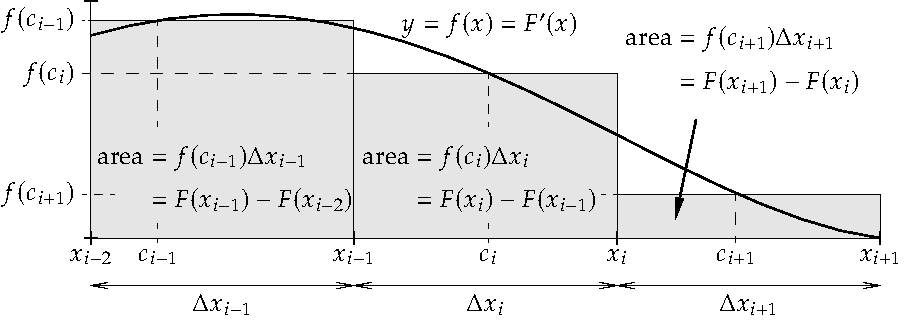
\includegraphics{figures/fundthmfig}
\caption{Mean value theorem on subintervals of a partition
approximating area under the curve.\label{fig:fundthmfig}}
\end{myfigureht}

Using the notation from the definition of the integral, we have
$m_i \leq f(c_i) \leq M_i$, and so
\begin{equation*}
m_i \Delta x_i \leq F(x_i) - F(x_{i-1}) \leq M_i \Delta x_i .
\end{equation*}
We sum over $i = 1,2, \ldots, n$ to get
\begin{equation*}
\sum_{i=1}^n m_i \Delta x_i
\leq \sum_{i=1}^n \bigl(F(x_i) - F(x_{i-1}) \bigr)
\leq \sum_{i=1}^n M_i \Delta x_i .
\end{equation*}
In the middle sum, all the terms except the first and last cancel 
and we end up with $F(x_n)-F(x_0) = F(b)-F(a)$.  The sums on the left
and on the right are the lower and the upper sum respectively.  So
\begin{equation*}
L(P,f) \leq F(b)-F(a) \leq U(P,f) .
\end{equation*}
We take the supremum of $L(P,f)$ over all partitions $P$ and the left inequality
yields 
\begin{equation*}
\underline{\int_a^b} f \leq F(b)-F(a) .
\end{equation*}
Similarly, taking
the infimum of $U(P,f)$ over all partitions $P$ yields
\begin{equation*}
F(b)-F(a) \leq \overline{\int_a^b} f .
\end{equation*}
As $f$ is Riemann integrable, we have
\begin{equation*}
\int_a^b f =
\underline{\int_a^b} f \leq F(b)-F(a) \leq \overline{\int_a^b} f
= \int_a^b f .
\end{equation*}
The inequalities must be equalities and we are done.
\end{proof}

The theorem is used to compute integrals.  Suppose we know that
the function $f(x)$ is a derivative of some other function $F(x)$,
then we can find an explicit expression for $\int_a^b f$. 

\begin{example}
Suppose we are trying to compute
\begin{equation*}
\int_0^1 x^2 ~dx .
\end{equation*}
We notice $x^2$ is the derivative of $\frac{x^3}{3}$.  We
use the fundamental theorem to write 
\begin{equation*}
\int_0^1 x^2 ~dx =
\frac{1^3}{3}
-
\frac{0^3}{3}
= \frac{1}{3}.
\end{equation*}
\end{example}

\subsection{Second form of the theorem}

The second form of the fundamental theorem gives us a way to solve
the differential equation $F'(x) = f(x)$, where $f$ is a known
function and we are trying to find an $F$ that satisfies the equation.

\begin{thm} \label{thm:FTCv2}
Let $f \colon [a,b] \to \R$ be a Riemann integrable function.  Define
\begin{equation*}
F(x) := \int_a^x f .
\end{equation*}
First, $F$ is continuous on $[a,b]$.  Second,
if $f$ is continuous at $c \in [a,b]$, then $F$ is differentiable at $c$
and $F'(c) = f(c)$.
\end{thm}

\begin{proof}
As $f$ is bounded, there is an $M > 0$
such that $\abs{f(x)} \leq M$ for all $x \in [a,b]$.  Suppose $x,y \in [a,b]$
with $x > y$.  Then
\begin{equation*}
\abs{F(x)-F(y)} =
\abs{\int_a^x f - \int_a^y f}
=
\abs{\int_y^x f}
\leq
M\abs{x-y} .
\end{equation*}
By symmetry, the same also holds if $x < y$.
So $F$ is Lipschitz continuous and hence continuous.

Now suppose $f$ is continuous at $c$.
Let $\epsilon > 0$ be given.  Let $\delta > 0$ be such that
for $x \in [a,b]$,
$\abs{x-c} < \delta$ implies $\abs{f(x)-f(c)} < \epsilon$.
In particular,
for such $x$ we have
\begin{equation*}
f(c)-\epsilon < f(x) < f(c) + \epsilon.
\end{equation*}
Thus if $x > c$, then
\begin{equation*}
\bigl(f(c)-\epsilon\bigr) (x-c) \leq \int_c^x f \leq
\bigl(f(c) + \epsilon\bigr)(x-c).
\end{equation*}
When $c > x$, then the inequalities are reversed.  Therefore,
assuming $c \not= x$ we get
\begin{equation*}
f(c)-\epsilon
\leq
\frac{\int_c^{x} f}{x-c}
\leq
f(c)+\epsilon .
\end{equation*}
As 
\begin{equation*}
\frac{F(x)-F(c)}{x-c}
=
\frac{\int_a^{x} f - \int_a^{c} f}{x-c}
=
\frac{\int_c^{x} f}{x-c} ,
\end{equation*}
we have 
\begin{equation*}
\abs{\frac{F(x)-F(c)}{x-c} - f(c)} \leq \epsilon .
\end{equation*}
The result follows.  It is left to the reader to see why is it OK that we
just have a non-strict inequality.
\end{proof}

Of course, if $f$ is continuous on $[a,b]$, then it is automatically Riemann
integrable, $F$ is differentiable on all of $[a,b]$ and $F'(x) = f(x)$ for
all $x \in [a,b]$.

\begin{remark} \label{remark:fundthmbase}
The second form of the fundamental theorem of calculus still holds if
we let $d \in [a,b]$ and define
\begin{equation*}
F(x) := \int_d^x f .
\end{equation*}
That is, we can use any point of $[a,b]$ as our base point.  The proof is
left as an exercise.
\end{remark}

Let us look at what a simple discontinuity can do.  Take $f(x) := -1$ if $x
< 0$, and $f(x) := 1$ if $x \geq 0$.  Let $F(x) := \int_0^x f$.  It is not
difficult to see that $F(x) = \abs{x}$.  Notice that $f$ is discontinuous at
$0$ and $F$ is not differentiable at $0$.  However, the converse in the
theorem does not
hold.
Let $g(x) := 0$ if $x \not= 0$, and $g(0) := 1$.  Letting $G(x) :=
\int_0^x g$, we find that $G(x) = 0$ for all $x$.  So $g$ is discontinuous
at $0$, but $G'(0)$ exists and is equal to 0.

A common misunderstanding of the integral for calculus students is to
think of integrals whose solution cannot be given in closed-form as somehow
deficient.  This is not the case.  Most integrals we write down are not
computable in closed-form.  Even some integrals that we consider
in closed-form are not really such.  We define
the natural logarithm as the antiderivative of $\nicefrac{1}{x}$
such that $\ln 1 = 0$:
\begin{equation*}
\ln x := \int_1^x \frac{1}{s}~ds .
\end{equation*}
So for example, how does a computer find
the value of $\ln x$?  One way to do it is to numerically approximate this integral.
Morally,
we did not really \myquote{simplify} $\int_1^x \nicefrac{1}{s}~ds$ by
writing down $\ln x$.  We simply gave the integral a name.
If we require numerical answers,
it is possible we end up doing
the calculation by approximating an integral anyway.
In the next section, we even define the exponential using
the logarithm, which we define in terms of the integral.

Another common function defined by an integral that cannot
be evaluated symbolically in terms of elementary functions
is the $\operatorname{erf}$ function, defined as
\begin{equation*}
\operatorname{erf}(x) := \frac{2}{\sqrt{\pi}} \int_0^x e^{-s^2} ~ds .
\end{equation*}
This function comes up often in applied mathematics.  It is simply 
the antiderivative of $\left(\nicefrac{2}{\sqrt{\pi}}\right) e^{-x^2}$
that is zero at zero.
The second form of the fundamental theorem tells us that we can write the function
as an integral.  If we wish to compute any particular value, we 
numerically approximate the integral.

\subsection{Change of variables}

A theorem often used in calculus to solve integrals is the change of
variables theorem, you may have called it \emph{$u$-substitution}.
Let us prove it now.  Recall 
a function is continuously differentiable if
it is differentiable and the derivative is continuous.

\begin{thm}[Change of variables]
\index{change of variables theorem}
Let $g \colon [a,b] \to \R$ be a continuously differentiable function,
let $f \colon [c,d] \to \R$ be continuous, and suppose
$g\bigl([a,b]\bigr) \subset [c,d]$.  Then
\begin{equation*}
\int_a^b f\bigl(g(x)\bigr)\, g'(x)~ dx =
\int_{g(a)}^{g(b)} f(s)~ ds .
\end{equation*}
\end{thm}

\begin{proof}
As $g$, $g'$, and $f$ are continuous, we know $f\bigl(g(x)\bigr)\,g'(x)$
is a continuous function on $[a,b]$, therefore it is Riemann integrable.
Similarly, $f$ is integrable on any subinterval of $[c,d]$.

Define 
\begin{equation*}
F(y) := \int_{g(a)}^{y} f(s)~ds .
\end{equation*}
By the second form of the fundamental
theorem of calculus (see \remarkref{remark:fundthmbase} and \exerciseref{secondftc:exercise})
$F$ is a differentiable function and $F'(y) = f(y)$.  We apply the chain
rule and write
\begin{equation*}
\bigl( F \circ g \bigr)' (x) =
F'\bigl(g(x)\bigr) g'(x)
=
f\bigl(g(x)\bigr) g'(x) .
\end{equation*}
We note that $F\bigl(g(a)\bigr) = 0$ and we
use the first form of the fundamental theorem
to obtain
\begin{multline*}
\qquad %to center things more
\int_{g(a)}^{g(b)} f(s)~ds = F\bigl(g(b)\bigr) = F\bigl(g(b)\bigr)-F\bigl(g(a)\bigr)
\\
=
\int_a^b 
\bigl( F \circ g \bigr)' (x) ~dx
=
\int_a^b 
f\bigl(g(x)\bigr) g'(x)
~dx .
\qquad %to center things more
\qedhere
\end{multline*}
\end{proof}

The change of variables theorem is often used to solve integrals by changing them
to integrals that we know or that we can solve using the fundamental theorem of
calculus.

\begin{example}
From an exercise, we know that the derivative of $\sin(x)$ is $\cos(x)$.
Therefore, we solve
\begin{equation*}
\int_0^{\sqrt{\pi}} x \cos(x^2) ~ dx = \int_0^\pi \frac{\cos(s)}{2} ~ ds
=
\frac{1}{2}
\int_0^\pi \cos(s) ~ ds
=
\frac{
\sin(\pi) - \sin(0)
}{2}
=
0 .
\end{equation*}
\end{example}

However, beware that we must satisfy the hypotheses of the theorem.  The
following example demonstrates why we should not just 
move symbols around mindlessly.
We must be careful that those symbols really make sense.

\begin{example}
Suppose we write down
\begin{equation*}
\int_{-1}^{1} \frac{\ln \abs{x}}{x} ~dx .
\end{equation*}
It may be tempting to take $g(x) := \ln \abs{x}$.  Then take $g'(x) =
\nicefrac{1}{x}$ and try to write
\begin{equation*}
\int_{g(-1)}^{g(1)} s ~ds = 
\int_{0}^{0} s ~ds = 0. 
\end{equation*}
This \myquote{solution} is incorrect, and it does not say
that we can solve the given integral.  First problem is that
$\frac{\ln \abs{x}}{x}$ is not continuous on $[-1,1]$.
It is not defined at 0, and cannot be made continuous by defining a value at
0.
Second, $\frac{\ln \abs{x}}{x}$ is not even Riemann integrable on $[-1,1]$
(it is unbounded).
The integral we wrote down simply does not make sense.
Finally, $g$ is not continuous 
on $[-1,1]$, let alone continuously differentiable.
\end{example}

\subsection{Exercises}

\begin{exercise}
Compute
$\displaystyle
\frac{d}{dx} \biggl( \int_{-x}^x e^{s^2}~ds \biggr)$.
\end{exercise}

\begin{exercise}
Compute
$\displaystyle
\frac{d}{dx} \biggl( \int_{0}^{x^2} \sin(s^2)~ds \biggr)$.
\end{exercise}

\begin{exercise}
Suppose $F \colon [a,b] \to \R$ is continuous and differentiable
on $[a,b] \setminus S$, where $S$ is a finite set.  Suppose there
exists an $f \in \sR[a,b]$ such that $f(x) = F'(x)$ for $x \in [a,b]
\setminus S$.  Show that
$\int_a^b f = F(b)-F(a)$.
\end{exercise}

\begin{exercise} \label{secondftc:exercise}
Let $f \colon [a,b] \to \R$ be a continuous function.  Let $c \in [a,b]$
be arbitrary.  Define
\begin{equation*}
F(x) := \int_c^x f .
\end{equation*}
Prove that $F$ is differentiable and that $F'(x) = f(x)$ for all $x \in
[a,b]$.
\end{exercise}

\begin{exercise}
Prove \emph{\myindex{integration by parts}}.  That is, suppose $F$ and
$G$ are continuously differentiable functions on $[a,b]$.  Then prove
\begin{equation*}
\int_a^b F(x)G'(x)~dx
=
F(b)G(b)-F(a)G(a)
-
\int_a^b F'(x)G(x)~dx .
\end{equation*}
\end{exercise}

\begin{exercise}
Suppose $F$ and $G$ are
continuously\footnote{
Compare this hypothesis to \exerciseref{exercise:samediffconst}.}
differentiable
functions defined on $[a,b]$
such that $F'(x) = G'(x)$ for all $x \in [a,b]$.
Using the fundamental theorem of calculus,
show that $F$ and $G$ differ by a constant.  That is, show that
there exists a $C \in \R$ such that
$F(x)-G(x) = C$.
\end{exercise}

\begin{exnote}
The next exercise shows how we can use the integral to \myquote{smooth out} a
non-differentiable function.
\end{exnote}

\begin{exercise} \label{exercise:smoothingout}
Let $f \colon [a,b] \to \R$ be a continuous function.  Let $\epsilon > 0$
be a constant.  For $x \in [a+\epsilon,b-\epsilon]$, define
\begin{equation*}
g(x) := \frac{1}{2\epsilon} \int_{x-\epsilon}^{x+\epsilon} f .
\end{equation*}
\begin{enumerate}[a)]
\item
Show that $g$ is differentiable and find the derivative.
\item
Let $f$ be differentiable and fix $x \in (a,b)$ (let $\epsilon$
be small enough).  What happens to $g'(x)$ as $\epsilon$ gets smaller?
\item
Find $g$ for $f(x) := \abs{x}$, $\epsilon = 1$ (you can assume 
$[a,b]$ is large enough).
\end{enumerate}
\end{exercise}

\begin{exercise}
Suppose $f \colon [a,b] \to \R$ is continuous and
$\int_a^x f = \int_x^b f$ for all $x \in [a,b]$.  Show that $f(x) = 0$
for all $x \in [a,b]$.
\end{exercise}

\begin{exercise}
Suppose $f \colon [a,b] \to \R$ is continuous and
$\int_a^x f = 0$ for all rational $x$ in $[a,b]$.  Show that $f(x) = 0$
for all $x \in [a,b]$.
\end{exercise}

\begin{samepage}
\begin{exercise}
A function $f$ is an \emph{\myindex{odd function}} if $f(x) = -f(-x)$,
and $f$ is an \emph{\myindex{even function}} if $f(x) = f(-x)$.  Let $a >
0$.  Assume $f$ is continuous.  Prove:
\begin{enumerate}[a)]
\item
If $f$ is odd, then $\int_{-a}^a f = 0$.
\item
If $f$ is even, then $\int_{-a}^a f = 2 \int_0^a f$.
\end{enumerate}
\end{exercise}
\end{samepage}

\begin{exercise}
\leavevmode
\begin{enumerate}[a)]
\item
Show that $f(x) := \sin(\nicefrac{1}{x})$
is integrable on any interval (you can define $f(0)$ to be anything).
\item
Compute $\int_{-1}^1 \sin(\nicefrac{1}{x})~dx$.  (Mind the
discontinuity.)
\end{enumerate}
\end{exercise}

\begin{exercise}[uses \sectionref{sec:monotonefunc}]
\leavevmode
\begin{enumerate}[a)]
\item
Suppose $f \colon [a,b] \to \R$ is increasing, by
\propref{prop:monotoneintegrable},
%\exerciseref{exercise:boundedvariationintegrable},
$f$ is Riemann integrable.  Suppose $f$ has a discontinuity at $c \in
(a,b)$, show that $F(x) := \int_a^x f$ is not differentiable at $c$.
\item
In \exerciseref{exercise:increasingfuncdiscatQ}, you constructed an increasing
function $f \colon [0,1] \to \R$ that is discontinuous at every
$x \in [0,1] \cap \Q$.  Use this $f$ to construct a function $F(x)$ that is
continuous on $[0,1]$, but not differentiable at every $x \in [0,1] \cap \Q$.
\end{enumerate}
\end{exercise}

%%%%%%%%%%%%%%%%%%%%%%%%%%%%%%%%%%%%%%%%%%%%%%%%%%%%%%%%%%%%%%%%%%%%%%%%%%%%%%

\sectionnewpage
\section{The logarithm and the exponential}
\label{sec:logandexp}

\sectionnotes{1 lecture (optional, requires the optional sections 
\sectionref{sec:limitatinf},
\sectionref{sec:monotonefunc},
\sectionref{sec:ift})}

We now have the tools required to properly define the exponential
and the
logarithm that you know from calculus so well.  We start with
exponentiation.
If $n$ is a positive integer, it is obvious to define
\begin{equation*}
x^n := \underbrace{x \cdot x \cdot \cdots \cdot x}_{n \text{ times}} .
\end{equation*}
It makes sense to define $x^0 := 1$.
For negative integers, let $x^{-n} := \nicefrac{1}{x^n}$.
If $x > 0$, define
$x^{1/n}$ as
the unique positive $n$th root.  Finally, for a rational
number $\nicefrac{n}{m}$ (in lowest terms), define
\begin{equation*}
x^{n/m} := {\bigl(x^{1/m}\bigr)}^n .
\end{equation*}
It is not difficult to show 
we get the same number no matter what
representation of $\nicefrac{n}{m}$ we use, so we do not need to use
lowest terms.

However, what do we mean by $\sqrt{2}^{\sqrt{2}}$?  Or
$x^y$ in general?  In particular, what is $e^x$ for all $x$?
And how do we solve $y=e^x$ for $x$?
This section answers these questions and more.

\subsection{The logarithm}
\index{logarithm}

It is convenient to define the logarithm first.
Let us show that
a unique function with the right properties exists, and only then will
we call it \emph{the} logarithm.

\begin{prop}
There exists a unique function $L \colon (0,\infty) \to \R$ such that
\begin{enumerate}[(i)]
\item \label{it:log:i}
$L(1) = 0$.
\item \label{it:log:ii}
$L$ is differentiable and $L'(x) = \nicefrac{1}{x}$.
\item \label{it:log:iii}
$L$ is strictly increasing, bijective, and
\begin{equation*}
\lim_{x\to 0} L(x) = -\infty , \qquad \text{and} \qquad
\lim_{x\to \infty} L(x) = \infty .
\end{equation*}
\item \label{it:log:iv}
$L(xy) = L(x)+L(y)$ for all $x,y \in (0,\infty)$.
\item \label{it:log:v}
If $q$ is a rational number and $x > 0$, then
$L(x^q) = q L(x)$.
\end{enumerate}
\end{prop}

\begin{proof}
To prove existence, we define a candidate and show it satisfies
all the properties.  Let
\begin{equation*}
L(x) := \int_1^x \frac{1}{t}~dt .
\end{equation*}

Obviously, \ref{it:log:i} holds.  Property \ref{it:log:ii} holds
via the second form of the fundamental theorem of calculus
(\thmref{thm:FTCv2}).

To prove property \ref{it:log:iv},
we change variables $u=yt$ to obtain
\begin{equation*}
L(x) =
\int_1^{x} \frac{1}{t}~dt
=
\int_y^{xy} \frac{1}{u}~du
=
\int_1^{xy} \frac{1}{u}~du
-
\int_1^{y} \frac{1}{u}~du
=
L(xy)-L(y) .
\end{equation*}

Let us prove \ref{it:log:iii}.
Property \ref{it:log:ii} together with the fact that $L'(x) = \nicefrac{1}{x} > 0$ 
for $x > 0$, implies that $L$
is strictly increasing and hence one-to-one.
Let us show $L$ is onto.  
As $\nicefrac{1}{t} \geq \nicefrac{1}{2}$ when $t \in [1,2]$,
\begin{equation*}
L(2) = \int_1^2 \frac{1}{t} ~dt \geq \nicefrac{1}{2} .
\end{equation*}
By induction, \ref{it:log:iv} implies that for $n \in \N$
\begin{equation*}
L(2^n) = L(2) + L(2) + \cdots + L(2) = n L(2) .
\end{equation*}
Given any $y > 0$, 
by the \hyperref[thm:arch:i]{Archimedean property} of the real numbers
(notice $L(2) > 0$), there is an $n \in \N$ such that
$L(2^n) > y$.  By the
\hyperref[IVT:thm]{intermediate value theorem}
there is an $x_1 \in (1,2^n)$ such that $L(x_1) = y$.  We get
$(0,\infty)$ is in the image of $L$.
As $L$ is increasing, $L(x) > y$ for all $x > 2^n$, and so
\begin{equation*}
\lim_{x\to\infty} L(x) = \infty .
\end{equation*}
Next
$0 = L(\nicefrac{x}{x}) = L(x) + L(\nicefrac{1}{x})$, and
so $L(x) = - L(\nicefrac{1}{x})$.  Using $x=2^{-n}$, we obtain
as above that $L$ achieves all negative numbers.  And
\begin{equation*}
\lim_{x \to 0} L(x) = 
\lim_{x \to 0} -L(\nicefrac{1}{x})
=
\lim_{x \to \infty} -L(x)
=  - \infty .
\end{equation*}
In the limits, note that only $x > 0$ are in the domain of $L$.

Let us prove \ref{it:log:v}.
Fix $x > 0$.
As above, \ref{it:log:iv} implies
$L(x^n) = n L(x)$
for all $n \in \N$.
We already found that
$L(x) = - L(\nicefrac{1}{x})$,
so $L(x^{-n}) = - L(x^n) = -n L(x)$.  Then for $m \in \N$
\begin{equation*}
L(x) = L\Bigl({(x^{1/m})}^m\Bigr) = m L\bigl(x^{1/m}\bigr) .
\end{equation*}
Putting everything together for $n \in \Z$ and $m \in \N$ we have
$L(x^{n/m}) = n L(x^{1/m}) = (\nicefrac{n}{m}) L(x)$.

Uniqueness follows using properties \ref{it:log:i} and
\ref{it:log:ii}.  Via the first form of the
fundamental theorem of calculus (\thmref{thm:FTCv1}),
\begin{equation*}
L(x) = \int_1^x \frac{1}{t}~dt
\end{equation*}
is the unique function such that $L(1) = 0$ and $L'(x) = \nicefrac{1}{x}$.
\end{proof}

Having proved
that there is a unique function with these properties,
we simply define the \emph{\myindex{logarithm}} or sometimes called the
\emph{\myindex{natural logarithm}}:
\glsadd{not:ln}
\begin{equation*}
\ln(x) := L(x) .
\end{equation*}

Mathematicians usually write $\log(x)$ instead of $\ln(x)$, which is
more familiar to calculus students.  For all practical purposes, there is only one logarithm:
the natural logarithm.  See \exerciseref{exercise:otherlogbases}.

\subsection{The exponential}
\index{exponential}

Just as with the logarithm we define the exponential via a list of
properties.

\begin{prop}
There exists a unique function $E \colon \R \to (0,\infty)$ such that
\begin{enumerate}[(i)]
\item \label{it:exp:i}
$E(0) = 1$.
\item \label{it:exp:ii}
$E$ is differentiable and $E'(x) = E(x)$.
\item \label{it:exp:iii}
$E$ is strictly increasing, bijective, and
\begin{equation*}
\lim_{x\to -\infty} E(x) = 0 , \qquad \text{and} \qquad
\lim_{x\to \infty} E(x) = \infty .
\end{equation*}
\item \label{it:exp:iv}
$E(x+y) = E(x)E(y)$ for all $x,y \in \R$.
\item \label{it:exp:v}
If $q \in \Q$, then
$E(qx) = {E(x)}^q$.
\end{enumerate}
\end{prop}

\begin{proof}
Again, we prove existence of such a function by defining a candidate
and proving that it satisfies all the properties.
The $L = \ln$ defined above is invertible.  Let $E$ be the
inverse function of $L$.  Property \ref{it:exp:i} is immediate.

Property \ref{it:exp:ii} follows
via the inverse function theorem, in particular
\lemmaref{lemma:ift}:  $L$ satisfies
all the hypotheses of the lemma, and hence
\begin{equation*}
E'(x) = \frac{1}{L'\bigl(E(x)\bigr)} = E(x) .
\end{equation*}

Let us look at property \ref{it:exp:iii}.
The function $E$ is strictly increasing since 
$E'(x) = E(x) > 0$.  As $E$ is the inverse of $L$, it must also
be bijective.  
To find the limits, we use that 
$E$ is strictly increasing and onto $(0,\infty)$.
For every $M > 0$, there is an $x_0$ such that
$E(x_0) = M$ and $E(x) \geq M$ for all $x \geq x_0$.
Similarly, for every $\epsilon > 0$, there is
an $x_0$ such that $E(x_0) = \epsilon$ and
$E(x) < \epsilon$ for all $x < x_0$.
Therefore,
\begin{equation*}
\lim_{n\to -\infty} E(x) = 0 , \qquad \text{and} \qquad
\lim_{n\to \infty} E(x) = \infty .
\end{equation*}

To prove property \ref{it:exp:iv}, we use the corresponding
property for the logarithm.
Take $x, y \in \R$.
As $L$ is bijective, find $a$ and $b$ such that $x = L(a)$ and $y = L(b)$.  Then
\begin{equation*}
E(x+y) =
E\bigl(L(a)+L(b)\bigr) = 
E\bigl(L(ab)\bigr) = ab = E(x)E(y)  .
\end{equation*}

Property \ref{it:exp:v} also follows from the corresponding property of $L$.
Given $x \in \R$, let $a$ be such that $x = L(a)$ and
\begin{equation*}
E(qx) = E\bigl(qL(a)\bigr)
=
E\bigl(L(a^q)\bigr) = a^q = {E(x)}^q .
\end{equation*}

Uniqueness follows from
\ref{it:exp:i} and
\ref{it:exp:ii}.
Let $E$ and $F$
be two functions satisfying
\ref{it:exp:i} and \ref{it:exp:ii}.  
\begin{equation*}
\frac{d}{dx} \Bigl( F(x)E(-x) \Bigr)
=
F'(x)E(-x) - E'(-x)F(x)
=
F(x)E(-x) - E(-x)F(x) = 0 .
\end{equation*}
Therefore, by \propref{prop:derzeroconst},
$F(x)E(-x) = F(0)E(-0) = 1$ for all $x \in \R$.
Next, $1 = E(0) = E(x-x) = E(x)E(-x)$.
%Doing the computation with $F = E$,
%we obtain $E(x)E(-x) = 1$.
Then
\begin{equation*}
0 = 1-1 = F(x)E(-x) - E(x)E(-x) = \bigl(F(x)-E(x)\bigr) E(-x) .
\end{equation*}
%Since $E(x)E(-x) = 1$,
Finally, $E(-x) \not= 0$\footnote{%
$E$ is a function into $(0,\infty)$ after all.
However, $E(-x) \neq 0$ also follows
from $E(x)E(-x) = 1$.  Therefore, we can prove uniqueness of $E$ 
given \ref{it:exp:i} and \ref{it:exp:ii}, even for functions $E \colon \R
\to \R$.}
for all $x \in \R$.
So
$F(x)-E(x) = 0$ for all $x$, and we are done.
\end{proof}

Having proved $E$ is unique, we define the
\emph{\myindex{exponential}} function as
\glsadd{not:exp}
\begin{equation*}
\exp(x) := E(x) .
\end{equation*}

If $y \in \Q$ and $x > 0$, then
\begin{equation*}
x^y = \exp\bigl(\ln(x^y)\bigr) = \exp\bigl(y\ln(x)\bigr) .
\end{equation*}
We can now make sense of exponentiation $x^y$ for arbitrary $y \in \R$;
if $x > 0$ and $y$ is irrational, define
\glsadd{not:pow}
\begin{equation*}
x^y := \exp\bigl(y\ln(x)\bigr) .
\end{equation*}
As $\exp$ is continuous, then $x^y$ is a continuous function of $y$.
Therefore, we would
obtain the same result had we taken a sequence of rational numbers $\{ y_n \}$
approaching $y$ and defined $x^y = \lim\, x^{y_n}$.

Define the number $e$,
sometimes called \emph{\myindex{Euler's number}} or
the \emph{\myindex{base of the natural logarithm}}, as
\glsadd{not:e}
\begin{equation*}
e := \exp(1) .
\end{equation*}
Let us justify the notation $e^x$ for $\exp(x)$:
\begin{equation*}
e^x = \exp\bigl(x \ln(e) \bigr) = \exp(x) .
\end{equation*}

The properties of the logarithm and the exponential extend to
irrational powers.  The proof is immediate.

\begin{prop}
Let $x, y \in \R$.
\begin{enumerate}[(i)]
\item
$\exp(xy) = {\bigl(\exp(x)\bigr)}^y$.
\item
If $x > 0$, then $\ln(x^y) = y \ln (x)$.
\end{enumerate}
\end{prop}

\begin{remark}
There are other equivalent ways to define the exponential and the logarithm.
A common way is to define $E$ as the solution to the differential equation
$E'(x) = E(x)$, $E(0) = 1$.  See \exampleref{example:picardexponential},
for a sketch of that approach.  Yet another
approach is to define the exponential function by
power series, see \exampleref{example:exponentialbypowerseries}.
\end{remark}

\begin{remark}
We proved the uniqueness of the functions $L$ and $E$ from
just the properties $L(1)=0$, $L'(x) = \nicefrac{1}{x}$
and the equivalent condition for the exponential
$E'(x) = E(x)$, $E(0) = 1$.  Existence also follows
from just these properties.
Alternatively, uniqueness also follows
from the laws of exponents, see the exercises.
\end{remark}

\subsection{Exercises}

\begin{exercise}
Let $y$ be any real number and $b > 0$.  Define $f \colon (0,\infty) \to \R$
and $g \colon \R \to \R$ as, $f(x) := x^y$ and $g(x) := b^x$.  Show that $f$
and $g$ are differentiable and find their derivative.
\end{exercise}

\begin{samepage}
\begin{exercise} \label{exercise:otherlogbases}
Let $b > 0$, $b\neq 1$ be given.
\begin{enumerate}[a)]
\item
Show that for every $y > 0$, there exists a unique number $x$
such that $y = b^x$.  Define
the \emph{\myindex{logarithm base $b$}},
$\log_b \colon (0,\infty) \to \R$, by
$\log_b(y) := x$.
\item
Show that $\log_b(x) = \frac{\ln(x)}{\ln(b)}$.
\item
Prove that if $c > 0$, $c \neq 1$, then
$\log_b(x) = \frac{\log_c(x)}{\log_c(b)}$.
\item
Prove $\log_b(xy) =
\log_b(x)+\log_b(y)$, and $\log_b(x^y) = y \log_b(x)$.
\end{enumerate}
\end{exercise}
\end{samepage}

\begin{exercise}[requires \sectionref{sec:taylor}]
Use \hyperref[thm:taylor]{Taylor's theorem} to study the remainder term and show that for
all $x \in \R$
\begin{equation*}
e^x = \sum_{n=0}^\infty \frac{x^n}{n!} .
\end{equation*}
Hint: Do not differentiate the series term by term (unless you would prove that it
works).
\end{exercise}

\begin{exercise}
Use the geometric sum formula to show (for $t\not= -1$)
\begin{equation*}
1-t+t^2-\cdots+{(-1)}^n t^n = \frac{1}{1+t} - \frac{{(-1)}^{n+1}t^{n+1}}{1+t}.
\end{equation*}
Using this fact show
\begin{equation*}
\ln (1+x) = \sum_{n=1}^\infty \frac{{(-1)}^{n+1}x^n}{n} 
\end{equation*}
for all $x \in (-1,1]$ (note that $x=1$ is included).  Finally,
find the limit of the alternating harmonic series
\begin{equation*}
\sum_{n=1}^\infty \frac{{(-1)}^{n+1}}{n} = 1 - \nicefrac{1}{2} +
\nicefrac{1}{3} - \nicefrac{1}{4} + \cdots
\end{equation*}
\end{exercise}

\begin{exercise}
Show 
\begin{equation*}
e^x = \lim_{n\to\infty} {\left( 1 + \frac{x}{n} \right)}^n .
\end{equation*}
Hint: Take the logarithm.\\
Note: The expression 
${\left( 1 + \frac{x}{n} \right)}^n$ arises in compound interest
calculations.  It is the amount of money in a bank account after 1 year
if 1 dollar was deposited initially at interest $x$
and the interest was compounded $n$
times during the year.  The exponential $e^x$ is the result of continuous
compounding.
\end{exercise}

\begin{samepage}
\begin{exercise}
\leavevmode
\begin{enumerate}[a)]
\item
Prove that for $n \in \N$,
\begin{equation*}
\sum_{k=2}^{n}
\frac{1}{k}
\leq
\ln (n)
\leq
\sum_{k=1}^{n-1}
\frac{1}{k} .
\end{equation*}
\item
Prove that the limit
\begin{equation*}
\gamma := \lim_{n\to\infty}
\left( \left( \sum_{k=1}^{n} \frac{1}{k} \right) - \ln (n) \right)
\end{equation*}
exists.  This constant is known as the
\emph{\myindex{Euler--Mascheroni constant}}%
\footnote{Named for the Swiss mathematician
\href{https://en.wikipedia.org/wiki/Leonhard_Euler}{Leonhard Paul Euler}
(1707--1783)
and the Italian mathematician
\href{https://en.wikipedia.org/wiki/Lorenzo_Mascheroni}{Lorenzo Mascheroni}
(1750--1800).}.  It is not known if this constant is rational or not.
It is approximately $\gamma \approx 0.5772$.
\end{enumerate}
\end{exercise}
\end{samepage}

\begin{exercise}
Show
\begin{equation*}
\lim_{x\to\infty} \frac{\ln(x)}{x} = 0 .
\end{equation*}
\end{exercise}

\begin{exercise}
Show that $e^x$ is \emph{\myindex{convex}}, in other words, show that 
if $a \leq x \leq b$, then
$e^x \leq e^a \frac{b-x}{b-a} + e^b \frac{x-a}{b-a}$.
\end{exercise}

\begin{exercise}
Using the logarithm find
\begin{equation*}
%\lim_{n\to\infty} {\left( 1 + \nicefrac{1}{n} \right)}^n = e .
\lim_{n\to\infty} n^{1/n} .
\end{equation*}
\end{exercise}

\begin{exercise}
Show that $E(x) = e^x$ is the unique continuous function such that
$E(x+y) = E(x)E(y)$ and $E(1) = e$.   Similarly, prove that $L(x) = \ln(x)$
is the unique continuous
function defined on positive $x$ such that $L(xy) = L(x)+L(y)$
and $L(e) = 1$.
\end{exercise}

\begin{exercise}[requires \sectionref{sec:taylor}]\label{exercise:nonanalytic}
Since $(e^x)' = e^x$, it is easy to see that $e^x$ is
\myindex{infinitely differentiable}\index{differentiable!infinitely}
(has derivatives of all orders).  Define the function $f \colon \R \to \R$.
\begin{equation*}
f(x) := \begin{cases}
e^{-1/x} & \text{if } x > 0, \\
0 & \text{if } x \leq 0.
\end{cases}
\end{equation*}
\begin{enumerate}[a)]
\item
Prove that for any $m \in \N$,
\begin{equation*}
\lim_{x \to 0^+} \frac{e^{-1/x}}{x^m} = 0 .
\end{equation*}
\item
Prove that $f$ is infinitely differentiable.
\item
Compute the Taylor series for $f$ at the origin, that is,
\begin{equation*}
\sum_{k=0}^\infty
\frac{f^{(k)}(0)}{k!}x^k .
\end{equation*}
Show that it converges, but show that it does not converge to $f(x)$
for any $x > 0$.
\end{enumerate}
\end{exercise}

%%%%%%%%%%%%%%%%%%%%%%%%%%%%%%%%%%%%%%%%%%%%%%%%%%%%%%%%%%%%%%%%%%%%%%%%%%%%%%

\sectionnewpage
\section{Improper integrals}
\label{sec:impropriemann}

\sectionnotes{2--3 lectures (optional section, can safely be skipped, 
requires the optional \sectionref{sec:limitatinf})}

Often it is necessary to integrate over the
entire real line, or an unbounded interval of the form $[a,\infty)$ or
$(-\infty,b]$.  We may also wish to integrate unbounded functions
defined on a open bounded interval $(a,b)$.
For such intervals or functions, the Riemann integral is not defined,
but we will write down
the integral anyway in the spirit of \lemmaref{lemma:boundedimpriemann}.
These integrals are called \emph{\myindex{improper integrals}}
and are limits
of integrals rather than integrals themselves.

\begin{defn}
Suppose $f \colon [a,b) \to \R$ is a function (not necessarily bounded)
that is Riemann integrable on $[a,c]$ for all $c < b$.  We define
\begin{equation*}
\int_a^b f := \lim_{c \to b^-} \int_a^{c} f ,
\end{equation*}
if the limit exists.

Suppose $f \colon [a,\infty) \to \R$ is a function such that
$f$ is Riemann integrable on $[a,c]$ for all $c < \infty$.  
We define
\begin{equation*}
\int_a^\infty f := \lim_{c \to \infty} \int_a^c f ,
\end{equation*}
if the limit exists.

If the limit exists, we say the improper integral
\emph{converges}\index{convergent!improper integral}.
If the limit does not exist, we say the improper integral
\emph{diverges}\index{divergent!improper integral}.

We similarly define improper integrals for the left-hand endpoint, we leave
this to the reader.
\end{defn}

For a finite endpoint $b$, if $f$ is bounded,
then
\lemmaref{lemma:boundedimpriemann} says that we defined nothing new.  What is new is that
we can apply this definition to unbounded functions.
The following set of examples is
so useful that we state it as a proposition.

\begin{prop}[$p$-test for integrals]%
\index{p-test for integrals@$p$-test for integrals}
\label{impropriemann:ptest}
The improper integral
\begin{equation*}
\int_1^\infty \frac{1}{x^p} ~dx
\end{equation*}
converges to $\frac{1}{p-1}$ if $p > 1$ and diverges if $0 < p \leq 1$.

The improper integral
\begin{equation*}
\int_0^1 \frac{1}{x^p} ~dx
\end{equation*}
converges to $\frac{1}{1-p}$ if $0 < p < 1$ and diverges if $p \geq 1$.
\end{prop}

\begin{proof}
The proof follows by application of the
\hyperref[thm:FTCv1]{fundamental theorem of calculus}.
Let us do the proof for $p > 1$ for the infinite right endpoint and
leave the rest to the reader.  Hint: You should handle $p=1$
separately.

Suppose $p > 1$.  Then
using the fundamental theorem,
\begin{equation*}
\int_1^b \frac{1}{x^p} ~dx
=
\int_1^b x^{-p} ~dx
=
\frac{b^{-p+1}}{-p+1}
-
\frac{1^{-p+1}}{-p+1}
=
\frac{-1}{(p-1)b^{p-1}}
+
\frac{1}{p-1} .
\end{equation*}
As $p > 1$, then $p-1 > 0$.  Take the limit as $b \to \infty$
to obtain that $\frac{1}{b^{p-1}}$ goes to 0.  The result follows.
\end{proof}

We state the following proposition on \myquote{tails} for just one type
of improper integral, though the proof is straight
forward and the same for other types of improper integrals.

\begin{prop} \label{impropriemann:tail}
Let $f \colon [a,\infty) \to \R$ be a function
that is Riemann integrable on $[a,b]$ for all $b > a$.
Given any $b > a$,
$\int_b^\infty f$ converges if and only if $\int_a^\infty f$
converges, in which case
\begin{equation*}
\int_a^\infty f
=
\int_a^b f +
\int_b^\infty f .
\end{equation*}
\end{prop}

\begin{proof}
Let $c > b$.  Then
\begin{equation*}
\int_a^c f
=
\int_a^b f +
\int_b^c f .
\end{equation*}
Taking the limit $c \to \infty$ finishes the proof.
\end{proof}

Nonnegative functions are easier to work with
as the following proposition demonstrates.
The exercises will show that this proposition
holds only for nonnegative functions.
Analogues of this proposition
exist for all the other types of improper limits and are left to the
student.

\begin{prop} \label{impropriemann:possimp}
Suppose $f \colon [a,\infty) \to \R$ is nonnegative ($f(x)
\geq 0$ for all $x$) and such that
$f$ is Riemann integrable on $[a,b]$ for all $b > a$.
\begin{enumerate}[(i)]
\item 
\begin{equation*}
\int_a^\infty f = \sup \left\{ \int_a^x f : x \geq a \right\} .
\end{equation*}
\item
Suppose $\{ x_n \}$
is a sequence with $\lim\, x_n = \infty$.  Then
$\int_a^\infty f$ converges if and only if $\lim\, \int_a^{x_n} f$ exists, in
which case
\begin{equation*}
\int_a^\infty f = \lim_{n\to\infty} \int_a^{x_n} f .
\end{equation*}
\end{enumerate}
\end{prop}

In the first item we allow for the value of $\infty$ in the
supremum indicating that the integral diverges to infinity.

\begin{proof}
We start with the first item.
As $f$ is nonnegative,
$\int_a^x f$ is increasing as a function of $x$.
If the supremum is infinite, then for every $M \in \R$
we find $N$ such that $\int_a^N f \geq M$.  As $\int_a^x f$
is increasing, $\int_a^x f \geq M$ for all $x \geq N$.  So
$\int_a^\infty f$ diverges to infinity.

Next suppose the supremum is finite, say
$A := \sup \left\{ \int_a^x f : x \geq a \right\}$.
For every $\epsilon > 0$, we find an $N$ such that
$A - \int_a^N f < \epsilon$.  As $\int_a^x f$ is increasing,
then
$A - \int_a^x f < \epsilon$ for all $x \geq N$ and hence
$\int_a^\infty f$ converges to $A$.

Let us look at the second item.
If $\int_a^\infty f$ converges, then every sequence $\{ x_n \}$ going to
infinity works.  The trick is
proving the other direction.  Suppose $\{ x_n \}$ is such that $\lim\, x_n =
\infty$ and
\begin{equation*}
\lim_{n\to\infty} \int_a^{x_n} f = A
\end{equation*}
converges.  Given $\epsilon > 0$, pick $N$ such that for
all $n \geq N$ we have
$A - \epsilon < \int_a^{x_n} f < A + \epsilon$.
Because $\int_a^x f$ is increasing as a function of $x$, we have that for all
$x \geq x_N$
\begin{equation*}
A - \epsilon < \int_a^{x_N} f \leq \int_a^x f .
\end{equation*}
As $\{ x_n \}$ goes to $\infty$, then for any given
$x$, there is an $x_m$ such that $m \geq N$ and $x \leq x_m$.  Then
\begin{equation*}
\int_a^{x} f \leq \int_a^{x_m} f < A + \epsilon .
\end{equation*}
In particular, for all $x \geq x_N$ we have
$\abs{\int_a^{x} f - A} < \epsilon$.
\end{proof}

\begin{prop}[\myindex{Comparison test for improper integrals}]
Let
$f \colon [a,\infty) \to \R$ and
$g \colon [a,\infty) \to \R$ be functions
that are Riemann integrable on $[a,b]$ for all $b > a$.   Suppose
that for all $x \geq a$ we have
\begin{equation*}
\abs{f(x)} \leq g(x) .
\end{equation*}
\begin{enumerate}[(i)]
\item If $\int_a^\infty g$ converges, then $\int_a^\infty f$ converges,
and in this case 
$\abs{\int_a^\infty f} \leq \int_a^\infty g$.
\item If $\int_a^\infty f$ diverges, then $\int_a^\infty g$ diverges.
\end{enumerate}
\end{prop}

\begin{proof}
Let us start with the first item.
For any $b$ and $c$, such that $a \leq b \leq c$, we have 
$-g(x) \leq f(x) \leq g(x)$, and so
\begin{equation*}
\int_b^c -g \leq \int_b^c f \leq \int_b^c g  .
\end{equation*}
In other words, $\abs{\int_b^c f} \leq \int_b^c g$.

Let $\epsilon > 0$ be given.  Because
of \propref{impropriemann:tail},
\begin{equation*}
\int_a^\infty g =
\int_a^b g +
\int_b^\infty g .
\end{equation*}
As $\int_a^b g$ goes to
$\int_a^\infty g$ as $b$ goes to infinity,
$\int_b^\infty g$ goes to 0 as $b$ goes to infinity.  Choose $B$
such that
\begin{equation*}
\int_B^\infty g < \epsilon .
\end{equation*}
As $g$ is nonnegative, if $B \leq b < c$, then
$\int_b^c g < \epsilon$ as well.
Let $\{ x_n \}$ be a sequence going to infinity.  Let $M$ be such that
$x_n \geq B$ for all $n \geq M$.  Take $n, m \geq M$,
with $x_n \leq x_m$,
\begin{equation*}
\abs{\int_a^{x_m} f - \int_a^{x_n} f} 
=
\abs{\int_{x_n}^{x_m} f} 
\leq \int_{x_n}^{x_m} g < \epsilon .
\end{equation*}
Therefore, the sequence $\{ \int_a^{x_n} f \}_{n=1}^\infty$ is Cauchy and hence converges.

We need to show that the limit is unique.  Suppose $\{ x_n \}$ is a sequence
converging to infinity such that
$\{ \int_a^{x_n} f \}$ converges to $L_1$, and $\{ y_n \}$ is a sequence
converging to infinity is such that
$\{ \int_a^{y_n} f \}$ converges to $L_2$.  Then there must be some $n$ such
that
$\abs{\int_a^{x_n} f - L_1} < \epsilon$ and 
$\abs{\int_a^{y_n} f - L_2} < \epsilon$.  We can also suppose $x_n \geq B$
and $y_n \geq B$.  Then
\begin{equation*}
\abs{L_1 - L_2} \leq
\abs{L_1 - \int_a^{x_n} f}
+
\abs{\int_a^{x_n} f- \int_a^{y_n} f}
+
\abs{\int_a^{y_n} f - L_2}
<
\epsilon
+
\abs{\int_{x_n}^{y_n} f}
+
\epsilon
<
3 \epsilon.
\end{equation*}
As $\epsilon > 0$ was arbitrary, $L_1 = L_2$, and hence
$\int_a^\infty f$ converges.
Above we have shown that $\abs{\int_a^c f} \leq \int_a^c g$ for all $c > a$.
By taking the limit $c \to \infty$, the first item is proved.

The second item is simply a contrapositive of the first item.
\end{proof}

\begin{example}
The improper integral
\begin{equation*}
\int_0^\infty \frac{\sin(x^2)(x+2)}{x^3+1} ~dx
\end{equation*}
converges.

Proof:  Observe we simply need to show
that the integral converges when going from 1 to infinity.
For $x \geq 1$ we obtain
\begin{equation*}
\abs{\frac{\sin(x^2)(x+2)}{x^3+1}}
\leq
\frac{x+2}{x^3+1}
\leq \frac{x+2}{x^3} \leq
\frac{x+2x}{x^3} \leq \frac{3}{x^2} .
\end{equation*}
Then
\begin{equation*}
\int_1^\infty \frac{3}{x^2}~dx
=
3 \int_1^\infty \frac{1}{x^2}~dx
%=
%\lim_{c\to\infty} \int_1^c \frac{3}{x^2} ~dx
=
3 .
\end{equation*}
So using the comparison test and the tail test, the original
integral converges.
\end{example}

\begin{example}
You should be careful when doing formal manipulations with improper
integrals.
The integral
\begin{equation*}
\int_2^\infty \frac{2}{x^2-1}~dx
\end{equation*}
converges via the comparison test using $\nicefrac{1}{x^2}$ again.  However, if you
succumb to the temptation to write
\begin{equation*}
\frac{2}{x^2-1} = 
\frac{1}{x-1}
-
\frac{1}{x+1} 
\end{equation*}
and try to integrate each part separately, you will not succeed.
It is \emph{not} true that you can split the improper
integral in two; you cannot split the limit.
\begin{equation*}
\begin{split}
\int_2^\infty \frac{2}{x^2-1} ~dx &=
\lim_{b\to \infty} \int_2^b \frac{2}{x^2-1} ~dx
\\
&=
\lim_{b\to \infty}
\left(
\int_2^b \frac{1}{x-1}~dx
-
\int_2^b \frac{1}{x+1}~dx
\right)
\\
&\not=
\int_2^\infty \frac{1}{x-1}~dx
-
\int_2^\infty \frac{1}{x+1}~dx .
\end{split}
\end{equation*}
The last line in the computation does not even make sense.  Both of the
integrals there diverge to infinity, since we can
apply the comparison test appropriately with
$\nicefrac{1}{x}$.  We get $\infty - \infty$.
\end{example}

Now suppose we need to take limits at both endpoints.

\begin{defn}
Suppose $f \colon (a,b) \to \R$ is a function
that is Riemann integrable on $[c,d]$ for all $c$, $d$
such that $a < c < d < b$, then we define
\begin{equation*}
\int_a^b f := \lim_{c \to a^+} \, \lim_{d \to b^-} \, \int_{c}^{d} f ,
\end{equation*}
if the limits exist.

Suppose $f \colon \R \to \R$ is a function such that
$f$ is Riemann integrable on all bounded intervals $[a,b]$.  Then
we define
\begin{equation*}
\int_{-\infty}^\infty f := \lim_{c \to -\infty} \, \lim_{d \to \infty} \, \int_c^d f ,
\end{equation*}
if the limits exist.

We similarly define improper integrals with one infinite and one finite
improper endpoint, we leave this to the reader.
\end{defn}

One ought to always be careful about double limits.  The definition
given above says that we first take the limit as $d$ goes to $b$ or
$\infty$ for a fixed $c$, and then we take the limit in $c$.
We will have to prove that in this case it does not matter which limit
we compute first.

\begin{example}
Let us see an example:
\begin{equation*}
\int_{-\infty}^\infty \frac{1}{1+x^2} ~ dx
=
\lim_{a \to -\infty} \, \lim_{b \to \infty} \,
\int_{a}^b \frac{1}{1+x^2} ~ dx
=
\lim_{a \to -\infty} \, \lim_{b \to \infty}
\bigl( \arctan(b) - \arctan(a) \bigr)
=
\pi .
\end{equation*}
\end{example}

In the definition the order of the limits can always be switched if they
exist.  Let us prove this fact only for the infinite limits.

\begin{prop}
If $f \colon \R \to \R$ is a function integrable on every bounded interval
$[a,b]$.
Then 
\begin{equation*}
\lim_{a \to -\infty} \, \lim_{b \to \infty} \, \int_a^b f
\quad \text{converges} \qquad \text{if and only if} \qquad
\lim_{b \to \infty}
\,
\lim_{a \to -\infty}
\,
\int_a^b f
\quad
\text{converges,}
\end{equation*}
in which case the two
expressions are equal.  If either of the
expressions converges, then the improper integral converges and
\begin{equation*}
\lim_{a\to\infty}
\int_{-a}^a f
=
\int_{-\infty}^\infty f .
\end{equation*}
\end{prop}

\begin{proof}
Without loss of generality assume $a < 0$ and $b > 0$.  Suppose
the first expression converges.  Then
\begin{equation*}
\begin{split}
\lim_{a \to -\infty} \, \lim_{b \to \infty} \, \int_a^b f
& =
\lim_{a \to -\infty} \, \lim_{b \to \infty}
\left(
\int_a^0 f
+
\int_0^b f
\right)
=
\left(
\lim_{a \to -\infty}
\int_a^0 f
\right)
+
\left(
 \lim_{b \to \infty}
\int_0^b f
\right) \\
& = 
 \lim_{b \to \infty}
\left(
\left(
\lim_{a \to -\infty}
\int_a^0 f
\right) 
+
\int_0^b f
\right)
=
 \lim_{b \to \infty} \,
\lim_{a \to -\infty}
\left(
\int_a^0 f
+
\int_0^b f
\right)  .
\end{split}
\end{equation*}
Similar computation shows the other direction.  Therefore, if
either expression converges, then the improper integral converges
and
\begin{equation*}
\begin{split}
\int_{-\infty}^\infty f
=
\lim_{a \to -\infty} \, \lim_{b \to \infty} \, \int_a^b f
& =
\left(
\lim_{a \to -\infty}
\int_a^0 f
\right)
+
\left(
 \lim_{b \to \infty}
\int_0^b f
\right)
\\
& =
\left(
\lim_{a \to \infty}
\int_{-a}^0 f
\right)
+
\left(
 \lim_{a \to \infty}
\int_0^a f
\right)
=
\lim_{a \to \infty}
\left(
\int_{-a}^0 f
+
\int_0^a f
\right)
=
\lim_{a \to \infty}
\int_{-a}^a f .
\end{split}
\end{equation*}
\end{proof}

\begin{example}
On the other hand, you must be careful to
take the limits independently before you know convergence.  Let
$f(x) = \frac{x}{\abs{x}}$ for $x \not= 0$ and $f(0) = 0$.
If $a < 0$ and $b > 0$, then
\begin{equation*}
\int_{a}^b f
=
\int_{a}^0 f
+
\int_{0}^b f
=
a+b .
\end{equation*}
For any fixed $a < 0$ the limit as $b \to \infty$ is infinite, so even
the first limit does not exist, and hence the improper integral
$\int_{-\infty}^\infty f$
does not converge.  On the other hand if $a > 0$, then
\begin{equation*}
\int_{-a}^{a} f
=
(-a)+a = 0 .
\end{equation*}
Therefore,
\begin{equation*}
\lim_{a\to\infty}
\int_{-a}^{a} f
= 0 .
\end{equation*}
\end{example}

\begin{example}
An example to keep in mind for improper integrals
is the so-called \emph{\myindex{sinc function}}%
\footnote{Shortened from Latin: \emph{sinus cardinalis}}.
This function comes up quite often
in both pure and applied mathematics.  Define
\begin{equation*}
\operatorname{sinc}(x) =
\begin{cases}
\frac{\sin(x)}{x} & \text{if } x \not= 0 , \\
1 & \text{if } x = 0 .
\end{cases}
\end{equation*}
\begin{myfigureht}
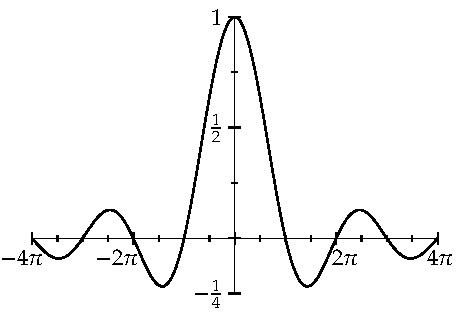
\includegraphics{figures/sincfig}
\caption{The sinc function.\label{figsinc}}
\end{myfigureht}

It is not difficult to show that
the sinc function is continuous at zero, but that is
not important right now.  What is important is that
\begin{equation*}
\int_{-\infty}^\infty \operatorname{sinc}(x) ~dx = \pi ,
\qquad \text{while} \qquad
\int_{-\infty}^\infty \abs{\operatorname{sinc}(x)} ~dx = \infty .
\end{equation*}
The integral of the sinc function is a continuous analogue of the
alternating harmonic series $\sum \nicefrac{{(-1)}^n}{n}$, while the
absolute value is like the regular harmonic series $\sum \nicefrac{1}{n}$.
In particular, the fact that the integral converges must be done directly
rather than using comparison test.

We will not prove the first statement exactly.  Let us simply prove
that the integral of the sinc function converges, but we will not worry
about the exact limit.  Because $\frac{\sin(-x)}{-x} = \frac{\sin(x)}{x}$, it is
enough to show that
\begin{equation*}
\int_{2\pi}^\infty \frac{\sin(x)}{x}~dx
\end{equation*}
converges.  We
also avoid $x=0$ this way to make our life simpler.

For any $n \in \N$, we have that for $x \in [\pi 2n, \pi (2n+1)]$
\begin{equation*}
\frac{\sin(x)}{\pi (2n+1)}
\leq
\frac{\sin(x)}{x}
\leq
\frac{\sin(x)}{\pi 2n} ,
\end{equation*}
as $\sin(x) \geq 0$.  On $x \in [\pi (2n+1), \pi (2n+2)]$
\begin{equation*}
\frac{\sin(x)}{\pi (2n+1)}
\leq
\frac{\sin(x)}{x}
\leq
\frac{\sin(x)}{\pi (2n+2)} ,
\end{equation*}
as $\sin(x) \leq 0$.

Via the fundamental theorem of calculus,
\begin{equation*}
\frac{2}{\pi (2n+1)}
=
\int_{\pi 2n}^{\pi (2n+1)}
\frac{\sin(x)}{\pi (2n+1)}
~dx
\leq
\int_{\pi 2n}^{\pi (2n+1)}
\frac{\sin(x)}{x}
~dx
\leq
\int_{\pi 2n}^{\pi (2n+1)}
\frac{\sin(x)}{\pi 2n}
~dx
=
\frac{1}{\pi n} .
\end{equation*}
Similarly,
\begin{equation*}
\frac{-2}{\pi (2n+1)}
\leq
\int_{\pi (2n+1)}^{\pi (2n+2)}
\frac{\sin(x)}{x}
~dx
\leq
\frac{-1}{\pi (n+1)} .
\end{equation*}
Adding the two together we find
\begin{equation*}
0
=
\frac{2}{\pi (2n+1)}
+
\frac{-2}{\pi (2n+1)}
\leq
\int_{2\pi n}^{2\pi (n+1)}
\frac{\sin(x)}{x}
~dx
\leq
\frac{1}{\pi n} 
+
\frac{-1}{\pi (n+1)} 
=
\frac{1}{\pi n(n+1)} .
\end{equation*}
See \figureref{fig:sincbound}.
\begin{myfigureht}
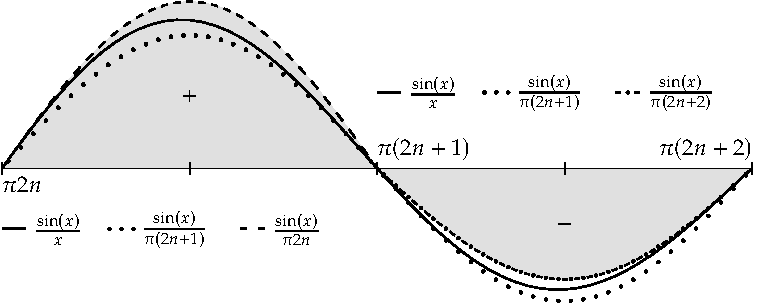
\includegraphics{figures/sincbound}
\caption{Bound of $\int_{2\pi n}^{2\pi (n+1)} \frac{\sin(x)}{x} ~dx$ using
the shaded integral (signed area
$\frac{1}{\pi n} 
+
\frac{-1}{\pi (n+1)}$).\label{fig:sincbound}}
\end{myfigureht}

For $k \in \N$, 
\begin{equation*}
\int_{2\pi}^{2k\pi} \frac{\sin(x)}{x} ~dx
=
\sum_{n=1}^{k-1}
\int_{2\pi n}^{2\pi (n+1)} \frac{\sin(x)}{x} ~dx 
\leq
\sum_{n=1}^{k-1}
\frac{1}{\pi n(n+1)} .
\end{equation*}
We find the partial sums of a series with positive terms.
The series
converges as
$\sum \frac{1}{\pi n (n+1)}$ is a convergent series.  Thus
as a sequence,
\begin{equation*}
\lim_{k\to \infty} \int_{2\pi}^{2k\pi} \frac{\sin(x)}{x} ~dx
=L \leq
\sum_{n=1}^{\infty}
\frac{1}{\pi n(n+1)} < \infty .
\end{equation*}

Let $M > 2\pi$ be arbitrary, and let $k \in \N$
be the largest integer such that $2k\pi \leq M$.
For $x \in [2k\pi,M]$ we have 
$\frac{-1}{2k\pi} \leq \frac{\sin(x)}{x} \leq \frac{1}{2k\pi}$, and so
\begin{equation*}
\abs{\int_{2k\pi}^{M} \frac{\sin(x)}{x} ~dx }  \leq
\frac{M-2k\pi}{2k\pi} \leq \frac{1}{k} .
\end{equation*}
As $k$ is the largest $k$ such that $2k\pi \leq M$,
then as $M\in \R$ goes to infinity, so does $k \in \N$.

Then
\begin{equation*}
\int_{2\pi}^M \frac{\sin(x)}{x}~dx
=
\int_{2\pi}^{2k\pi} \frac{\sin(x)}{x} ~dx
+
\int_{2k\pi}^{M} \frac{\sin(x)}{x} ~dx .
\end{equation*}
As $M$ goes to infinity,
the first term on the
right hand side goes to $L$,
and the second term on the
right hand side
goes to zero.  Hence
\begin{equation*}
\int_{2\pi}^\infty \frac{\sin(x)}{x} ~dx = L .
%\leq \sum_{n=1}^{\infty}
%\frac{1}{\pi n(n+1)} < \infty .
\end{equation*}

The double sided integral of sinc also exists as noted above.
We leave the other statement---that the integral
of the absolute value of the sinc function diverges---as an exercise.
\end{example}

\subsection{Integral test for series}

The fundamental theorem 
of calculus can be used in proving a series is summable and to estimate its sum.

\begin{prop}[Integral test]\index{integral test for series}
Suppose $f \colon [k,\infty) \to \R$ is a decreasing nonnegative
function where $k \in \Z$.  Then
\begin{equation*}
\sum_{n=k}^\infty f(n)
\quad \text{converges} \qquad \text{if and only if}
\qquad
\int_k^\infty f
\quad \text{converges}.
\end{equation*}
In this case 
\begin{equation*}
\int_k^\infty f
\leq
\sum_{n=k}^\infty f(n)
\leq
f(k)+
\int_k^\infty f .
\end{equation*}
\end{prop}
See \figureref{fig:integraltest}, for an illustration with $k=1$.
By \propref{prop:monotoneintegrable},
$f$ is integrable
on every interval $[k,b]$ for all $b > k$, so the statement of the theorem
makes sense without additional hypotheses of integrability.
\begin{myfigureht}
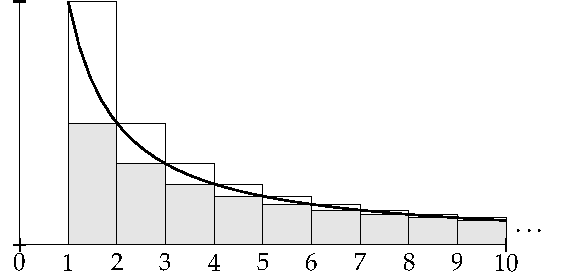
\includegraphics{figures/integraltest}
\caption{The area under the curve, 
$\int_1^\infty f$, is bounded below
by the area of the shaded rectangles,
$f(2)+f(3)+f(4)+\cdots$, and bounded above
by the area entire rectangles,
$f(1)+f(2)+f(3)+\cdots$.\label{fig:integraltest}}
\end{myfigureht}

\begin{proof}
Let $\ell, m \in \Z$ be such that $m > \ell \geq k$.
Because $f$ is decreasing, we have
$\int_{n}^{n+1} f \leq f(n) \leq \int_{n-1}^{n} f$.  Therefore,
\begin{equation} \label{impropriemann:eqseries}
\int_\ell^m f
=
\sum_{n=\ell}^{m-1} \int_{n}^{n+1} f
\leq
\sum_{n=\ell}^{m-1} f(n)
\leq
f(\ell) +
\sum_{n=\ell+1}^{m-1} \int_{n-1}^{n} f
\leq
f(\ell)+
\int_\ell^{m-1} f .
\end{equation}

Suppose first that $\int_k^\infty f$ converges and
let $\epsilon > 0$ be given.
As before, since $f$ is positive, then there exists
an $L \in \N$ such that if $\ell \geq L$, then
$\int_\ell^{m} f < \nicefrac{\epsilon}{2}$ for all $m \geq \ell$.
The function 
$f$ must decrease to zero (why?), so make $L$ large enough so that
for $\ell \geq L$ we have $f(\ell) < \nicefrac{\epsilon}{2}$.
Thus, for $m > \ell \geq L$, we have
via \eqref{impropriemann:eqseries},
\begin{equation*}
\sum_{n=\ell}^{m} f(n)
\leq
f(\ell)+
\int_\ell^{m} f < \nicefrac{\epsilon}{2} + \nicefrac{\epsilon}{2} = \epsilon .
\end{equation*}
The series is therefore Cauchy and thus converges.  The estimate in the
proposition is obtained by letting $m$ go to infinity in
\eqref{impropriemann:eqseries} with $\ell = k$.

Conversely, suppose $\int_k^\infty f$ diverges.  
As $f$ is positive, then by
\propref{impropriemann:possimp},
the sequence $\{ \int_k^m f \}_{m=k}^\infty$ diverges to infinity.
Using
\eqref{impropriemann:eqseries} with $\ell = k$, we find
\begin{equation*}
\int_k^m f
\leq
\sum_{n=k}^{m-1} f(n) .
\end{equation*}
As the left hand side goes to infinity as $m \to \infty$, so does the right
hand side.
\end{proof}

\begin{example}
The integral test can be used not only to show that a series converges, but to
estimate its sum to arbitrary precision.
Let us show $\sum_{n=1}^\infty \frac{1}{n^2}$ exists and
estimate its sum to within 0.01.  As this series is the $p$-series for
$p=2$, we already proved it converges (let us pretend we do not know that),
but we only roughly estimated its sum.

The fundamental theorem of calculus says that for $k \in \N$
we have
\begin{equation*}
\int_{k}^\infty \frac{1}{x^2}~dx = \frac{1}{k} .
\end{equation*}
In particular, the series must converge.  But we also have
\begin{equation*}
\frac{1}{k} = \int_k^\infty \frac{1}{x^2}~dx
\leq
\sum_{n=k}^\infty \frac{1}{n^2}
\leq
\frac{1}{k^2}
+
\int_k^\infty \frac{1}{x^2}~dx
=
\frac{1}{k^2}
+
\frac{1}{k} .
\end{equation*}
Adding the partial sum up to $k-1$ we get
\begin{equation*}
\frac{1}{k} + \sum_{n=1}^{k-1} \frac{1}{n^2}
\leq
\sum_{n=1}^\infty \frac{1}{n^2}
\leq
\frac{1}{k^2}
+
\frac{1}{k} + \sum_{n=1}^{k-1} \frac{1}{n^2} .
\end{equation*}
In other words,
$\nicefrac{1}{k} + \sum_{n=1}^{k-1} \nicefrac{1}{n^2}$ is an estimate for
the sum to within $\nicefrac{1}{k^2}$.  Therefore, if we wish to
find the sum to within 0.01, we note $\nicefrac{1}{{10}^2} = 0.01$.  We
obtain
\begin{equation*}
1.6397\ldots
\approx
\frac{1}{10} + \sum_{n=1}^{9} \frac{1}{n^2}
\leq
\sum_{n=1}^\infty \frac{1}{n^2}
\leq
\frac{1}{100}
+
\frac{1}{10} + \sum_{n=1}^{9} \frac{1}{n^2}
\approx
1.6497\ldots .
\end{equation*}
The actual sum is $\nicefrac{\pi^2}{6} \approx 1.6449\ldots$. 
\end{example}

\subsection{Exercises}

\begin{exercise}
Finish the proof of \propref{impropriemann:ptest}.
\end{exercise}

\begin{exercise}
Find out for which $a \in \R$ does $\sum\limits_{n=1}^\infty e^{an}$ converge.
When the series converges, find an upper bound for the sum.
\end{exercise}

\begin{exercise}
\leavevmode
\begin{enumerate}[a)]
\item
Estimate $\sum\limits_{n=1}^\infty \frac{1}{n(n+1)}$ correct to within 0.01
using the integral test.
\item
Compute the limit of the series exactly
and compare.  Hint: The sum telescopes.
\end{enumerate}
\end{exercise}

\begin{exercise}
Prove 
\begin{equation*}
\int_{-\infty}^\infty \abs{\operatorname{sinc}(x)}~dx = \infty .
\end{equation*}
Hint: Again, it is enough to show this on just one side.
\end{exercise}

\begin{exercise}
Can you interpret
\begin{equation*}
\int_{-1}^1 \frac{1}{\sqrt{\abs{x}}}~dx
\end{equation*}
as an improper integral?  If so, compute its value.
\end{exercise}

\begin{exercise}
Take $f \colon [0,\infty) \to \R$, Riemann integrable on
every interval $[0,b]$, and such that there exist $M$, $a$, and $T$,
such that $\abs{f(t)} \leq M e^{at}$ for all $t \geq T$.  Show that the
\emph{\myindex{Laplace transform}} of $f$ exists.  That is, for
every $s > a$ the following integral converges:
\begin{equation*}
F(s) := \int_{0}^\infty f(t) e^{-st} ~dt .
\end{equation*}
\end{exercise}

\begin{exercise}
Let $f \colon \R \to \R$ be a Riemann integrable function
on every interval $[a,b]$, and such
that $\int_{-\infty}^\infty \abs{f(x)}~dx < \infty$.  Show that the
\emph{\myindex{Fourier sine and cosine transforms}}
exist.  That is, for every $\omega \geq 0$ the
following integrals converge
\begin{equation*}
F^s(\omega) := \frac{1}{\pi} \int_{-\infty}^\infty f(t) \sin(\omega t) ~dt ,
\qquad
F^c(\omega) := \frac{1}{\pi} \int_{-\infty}^\infty f(t) \cos(\omega t) ~dt .
\end{equation*}
Furthermore, show that $F^s$ and $F^c$ are bounded functions.
\end{exercise}

\begin{exercise}
Suppose $f \colon [0,\infty) \to \R$ is Riemann integrable on every interval
$[0,b]$.  Show that  $\int_0^\infty f$ converges if and only if
for every $\epsilon > 0$ there exists an $M$ such that if $M \leq a < b$,
then $\babs{\int_a^b f} < \epsilon$.
\end{exercise}

\begin{exercise}
Suppose $f \colon [0,\infty) \to \R$ is nonnegative and
\emph{decreasing}.  Prove:
\begin{enumerate}[a)]
\item
If $\int_0^\infty f < \infty$, then $\lim\limits_{x\to\infty} f(x) = 0$.
\item
The converse does not hold.
\end{enumerate}
\end{exercise}

\begin{exercise}
Find an example of an \emph{unbounded} continuous function $f \colon
[0,\infty) \to \R$ that is nonnegative and such that $\int_0^\infty f < \infty$.
Note that $\lim_{x\to\infty} f(x)$ will not exist; compare
previous exercise.
Hint: On each interval $[k,k+1]$, $k \in \N$, define a function whose
integral over this interval is less than say $2^{-k}$.
\end{exercise}

\begin{exercise}[More challenging]
Find an example of a function $f \colon [0,\infty) \to \R$ integrable on all
intervals such that $\lim_{n\to\infty} \int_0^n f$ converges as a
limit of a sequence (so $n \in \N$), but such that
$\int_0^\infty f$ does not exist.
Hint: For all $n\in \N$, divide $[n,n+1]$ into two halves.  On one half
make the function negative, on the other make the function positive.
\end{exercise}

\begin{exercise}
Suppose $f \colon [1,\infty) \to \R$ is such that
$g(x) := x^2 f(x)$ is a bounded function. Prove that
$\int_1^\infty f$ converges.
\end{exercise}

\begin{exnote}
It is sometimes desirable to assign a value to integrals that normally
cannot be interpreted even as improper integrals,
e.g.\ $\int_{-1}^1 \nicefrac{1}{x}~dx$.
Suppose $f \colon [a,b] \to \R$ is a function and $a < c < b$,
where $f$ is Riemann integrable on the intervals
$[a,c-\epsilon]$ and $[c+\epsilon,b]$ for all $\epsilon > 0$.
Define
the \emph{\myindex{Cauchy principal value}} of $\int_a^b f$ as
\begin{equation*}
p.v.\!\int_a^b f := \lim_{\epsilon\to 0^+}
\left(
\int_a^{c-\epsilon} f + 
\int_{c+\epsilon}^b f
\right) ,
\end{equation*}
if the limit exists.
\end{exnote}

%\begin{samepage}
\begin{exercise}
\leavevmode
\begin{enumerate}[a)]
\item
Compute $p.v.\!\int_{-1}^1 \nicefrac{1}{x}~dx$.
\item
Compute
$\lim_{\epsilon\to 0^+}
( \int_{-1}^{-\epsilon} \nicefrac{1}{x}~dx + 
\int_{2\epsilon}^1 \nicefrac{1}{x}~dx )$ and show it is not equal
to the principal value.
\item
Show that if $f$ is integrable on $[a,b]$, then
$p.v.\!\int_a^b f = \int_a^b f$ (for an arbitrary $c \in (a,b)$).
\item
Suppose $f \colon [-1,1] \to \R$
is an odd function ($f(-x)=-f(x)$) that is integrable on
$[-1,-\epsilon]$ and $[\epsilon,1]$ for all $\epsilon >0$.
Prove that 
$p.v.\!\int_{-1}^1 f = 0$
\item
Suppose 
$f \colon [-1,1] \to \R$ is continuous and differentiable at 0.  Show that
$p.v.\!\int_{-1}^1 \frac{f(x)}{x}~dx$ exists.
\end{enumerate}
\end{exercise}
%\end{samepage}

\begin{samepage}
\begin{exercise}
Let $f \colon \R \to \R$ and 
$g \colon \R \to \R$ be continuous functions, where
$g(x) = 0$ for all $x \notin [a,b]$ for some interval $[a,b]$.
\begin{enumerate}[a)]
\item
Show that the
\emph{\myindex{convolution}}
\begin{equation*}
(g * f)(x) := \int_{-\infty}^\infty f(t)g(x-t)~dt 
\end{equation*}
is well-defined for all $x \in \R$.
\item
Suppose $\int_{-\infty}^\infty \abs{f(x)}~dx < \infty$.  Prove that
\begin{equation*}
\lim_{x \to -\infty} (g * f)(x) = 0, \qquad \text{and} \qquad
\lim_{x \to \infty} (g * f)(x) = 0 .
\end{equation*}
\end{enumerate}
\end{exercise}
\end{samepage}


%%%%%%%%%%%%%%%%%%%%%%%%%%%%%%%%%%%%%%%%%%%%%%%%%%%%%%%%%%%%%%%%%%%%%%%%%%%%%%

% Sequences of Functions chapter
\chapter{Sequences of Functions} \label{fs:chapter}

%%%%%%%%%%%%%%%%%%%%%%%%%%%%%%%%%%%%%%%%%%%%%%%%%%%%%%%%%%%%%%%%%%%%%%%%%%%%%%

\section{Pointwise and uniform convergence}
\label{sec:puconv}

\sectionnotes{1--1.5 lecture}

Up till now, when we talked about sequences we always talked about
sequences of numbers.  However, a very useful concept in analysis is to use a
sequence of functions.  For example, a solution to some
differential equation
might be found by finding only approximate solutions.  Then the real solution is
some sort of limit of those approximate solutions.

When talking about sequences of functions, the 
tricky part is that there are multiple notions of a limit.
Let us describe two common
notions of a limit of a sequence of functions.

\subsection{Pointwise convergence}

\begin{defn}
\index{pointwise convergence}
For every $n \in \N$
let $f_n \colon S \to \R$ be a function.  We say the sequence
$\{ f_n \}_{n=1}^\infty$
\emph{\myindex{converges pointwise}} to $f \colon S \to \R$ if for every $x
\in S$,
we have
\begin{equation*}
f(x) =
\lim_{n\to\infty} f_n(x) .
\end{equation*}
\end{defn}

As limits of sequences of numbers are unique, given a sequence $\{ f_n \}$ that
converges pointwise, the limit function $f$ is unique.
It is common to say that $f_n \colon S \to \R$
\emph{converges to $f$ on $T \subset S$}
for some $f \colon T \to \R$.  In that case we mean 
$f(x) = \lim\, f_n(x)$ for every $x \in T$.  In other words, the
restrictions of $f_n$ to $T$ converge pointwise to $f$.


\begin{example}
On $[-1,1]$ the sequence of functions defined by $f_n(x) := x^{2n}$
converges pointwise to $f \colon [-1,1] \to \R$, where
\begin{equation*}
f(x) =
\begin{cases}
1 & \text{if } x=-1 \text{ or } x=1, \\
0 & \text{otherwise.}
\end{cases}
\end{equation*}
See \figureref{x2nfig}.

\begin{myfigureht}
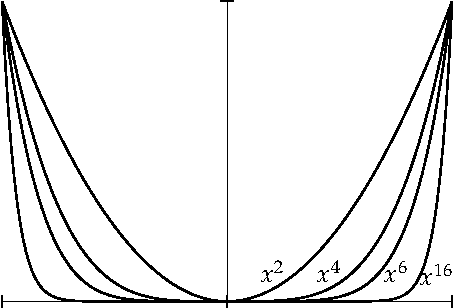
\includegraphics{figures/x2nfig}
\caption{Graphs of $f_1$, $f_2$, $f_3$, and $f_8$ for $f_n(x) :=
x^{2n}$.\label{x2nfig}}
\end{myfigureht}

To see this is so, first take $x \in (-1,1)$.  Then 
$0 \leq x^2 < 1$.
We have seen before that
\begin{equation*}
\abs{x^{2n} - 0} = {(x^2)}^n \to 0 \quad \text{as} \quad n \to \infty .
\end{equation*}
Therefore $\lim\,f_n(x) = 0$.

When $x = 1$ or $x=-1$, then $x^{2n} = 1$ for all $n$ and hence
$\lim\,f_n(x) = 1$.
For all other $x$, the sequence
$\{ f_n(x) \}$ does not converge.
\end{example}

Often, functions are given as a series.  In this case, we use
the notion of pointwise convergence to find the values of the function.

\begin{example} \label{example:geomsumptconv}
We write
\begin{equation*}
\sum_{k=0}^\infty x^k
\end{equation*}
to denote the limit of the functions
\begin{equation*}
f_n(x) := \sum_{k=0}^n x^k .
\end{equation*}
When studying series, 
we saw that on $x \in (-1,1)$ the $f_n$ converge pointwise to
\begin{equation*}
\frac{1}{1-x} .
\end{equation*}

The subtle point here is that while
$\frac{1}{1-x}$ is defined for all $x \not=1$, and $f_n$ are 
defined for all $x$ (even at $x=1$), convergence only happens on $(-1,1)$.

Therefore, when we write
\begin{equation*}
f(x) := \sum_{k=0}^\infty x^k
\end{equation*}
we mean that $f$ is defined on $(-1,1)$ and is the pointwise limit
of the partial sums.
\end{example}

\begin{example}
Let $f_n(x) := \sin(nx)$.  Then $f_n$ does not converge pointwise
to any function on any interval.  It may converge at certain points, such
as when $x=0$ or $x=\pi$.  It is left as an exercise that in any interval
$[a,b]$, there exists an $x$ such that $\sin(xn)$ does not have a limit
as $n$ goes to infinity.  See \figureref{fig:nonconvsinxn}.
\begin{myfigureht}
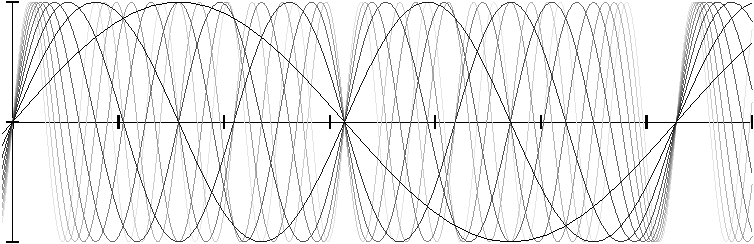
\includegraphics{figures/nonconvsinxn}
\caption{Graphs of $\sin(nx)$ for
$n=1,2,\ldots,10$, with higher $n$ in lighter gray.%
\label{fig:nonconvsinxn}}
\end{myfigureht}
\end{example}

Before we move to uniform convergence, let us reformulate pointwise
convergence in a different way.
We leave the proof to the reader, it is a simple application of the
definition of convergence of a sequence of real numbers.

\begin{prop} \label{ptwsconv:prop}
Let $f_n \colon S \to \R$ and $f \colon S \to \R$ be functions.
Then $\{ f_n \}$ converges pointwise to $f$ if and only if
for every $x \in S$, and every $\epsilon > 0$, there exists
an $N \in \N$ such that for all
$n \geq N$, we have
\begin{equation*}
\abs{f_n(x)-f(x)} < \epsilon .
\end{equation*}
\end{prop}

The key point here is that $N$ can depend on $x$, not just on
$\epsilon$.  That is, for each $x$ we can pick a different $N$.
If we can pick one $N$ for all $x$, we have what is called
uniform convergence.

\subsection{Uniform convergence}

\begin{defn}
\index{uniform convergence}
Let $f_n \colon S \to \R$
and $f \colon S \to \R$
be functions.  We say the sequence $\{ f_n \}$
\emph{\myindex{converges uniformly}} to $f$ if for
every $\epsilon > 0$ there exists an $N \in \N$ such that 
for all $n \geq N$, we have
\begin{equation*}
\abs{f_n(x) - f(x)} < \epsilon \qquad \text{for all } x \in S.
\end{equation*}
\end{defn}

In uniform convergence, $N$ cannot depend on $x$.  Given $\epsilon > 0$,
we must find an $N$ that works for all $x \in S$.  See
\figureref{fig:uniformconv} for an illustration.
\begin{myfigureht}
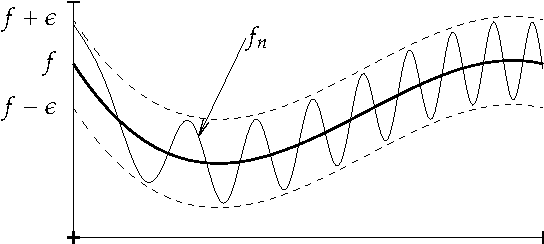
\includegraphics{figures/uniformconv}
\caption{In uniform convergence,
for $n \geq N$,
the functions $f_n$ are within a strip of $\pm\epsilon$ from $f$.%
\label{fig:uniformconv}}
\end{myfigureht}

Uniform convergence
implies pointwise convergence, and the proof follows by
\propref{ptwsconv:prop}:

\begin{prop}
Let $\{ f_n \}$ be a sequence of functions $f_n \colon S \to \R$.
If $\{ f_n \}$ converges
uniformly to $f \colon S \to \R$, then $\{ f_n \}$ converges pointwise to $f$.
\end{prop}

The converse does not hold.

\begin{example}
The functions $f_n(x) := x^{2n}$ do not converge uniformly on $[-1,1]$,
even though they converge pointwise.  To see this, suppose for contradiction
that the convergence is uniform.  For $\epsilon := \nicefrac{1}{2}$, there would have
to exist an $N$ such that $x^{2N} = \abs{x^{2N} - 0} < \nicefrac{1}{2}$ for all $x \in
(-1,1)$ (as $f_n(x)$ converges to 0 on $(-1,1)$).  But that means that
for every sequence $\{ x_k \}$ in $(-1,1)$ such that $\lim\, x_k = 1$,
we have $x_k^{2N} < \nicefrac{1}{2}$ for all $k$.  On the other hand,
$x^{2N}$ is a continuous function of $x$ (it is a polynomial).  Therefore,
we obtain a contradiction
\begin{equation*}
1 = 1^{2N}  = \lim_{k\to\infty} x_k^{2N} \leq \nicefrac{1}{2} .
\end{equation*}

However, if we restrict our domain to $[-a,a]$ where $0 < a < 1$, then
$\{ f_n \}$ converges uniformly to 0 on $[-a,a]$.  First note
that $a^{2n} \to 0$ as $n \to \infty$.  Thus given $\epsilon > 0$,
pick $N \in \N$ such that
$a^{2n} < \epsilon$ for all $n \geq N$.
Then $\abs{x} \leq a$ for all $x \in [-a,a]$.
Therefore, for $n \geq N$,
\begin{equation*}
\abs{x^{2n}} = \abs{x}^{2n} \leq a^{2n} < \epsilon .
\end{equation*}
\end{example}

\subsection{Convergence in uniform norm}

For bounded functions there is another more abstract way to 
think of uniform convergence.  To every bounded function we assign
a certain nonnegative number (called the uniform norm).  This number
measures the \myquote{distance} of the function from 0.  We can then
\myquote{measure}
how far two functions are from each other.  We then translate
a statement about uniform convergence into a statement about a certain
sequence of real numbers converging to zero.

\begin{defn} \label{def:unifnorm}
Let $f \colon S \to \R$ be a bounded function.  Define
\glsadd{not:uniformnorm}
\begin{equation*}
\norm{f}_u :=
\sup \bigl\{ \abs{f(x)} : x \in S \bigr\} .
\end{equation*}
We call $\norm{\cdot}_u$ the \emph{\myindex{uniform norm}}.
\end{defn}

To use this notation%
\footnote{The notation nor terminology is not completely standardized.  The norm is
also called the
\emph{\myindex{sup norm}} or
\emph{\myindex{infinity norm}}, and in addition
to $\norm{f}_u$ and $\norm{f}_S$ it is sometimes written
as $\norm{f}_{\infty}$ or $\norm{f}_{\infty,S}$.}
and this concept, the domain $S$ must be fixed.  Some authors
use
the notation
$\norm{f}_S$ to emphasize the dependence on $S$.

\begin{prop}
A sequence of bounded functions $f_n \colon S \to \R$ converges
uniformly to $f \colon S \to \R$, if and only if
\begin{equation*}
\lim_{n\to\infty} \norm{f_n - f}_u = 0 .
\end{equation*}
\end{prop}

\begin{proof}
First suppose 
$\lim \norm{f_n - f}_u = 0$.  Let $\epsilon > 0$ be
given.  Then there exists an $N$ such that
for $n \geq N$, we have $\norm{f_n - f}_u < \epsilon$.  As $\norm{f_n-f}_u$
is the supremum of $\abs{f_n(x)-f(x)}$, we see that for all $x \in S$,
we have $\abs{f_n(x)-f(x)} \leq \norm{f_n - f}_u < \epsilon$.

On the other hand, suppose $\{ f_n \}$ converges uniformly to $f$.
Let $\epsilon > 0$ be given.  Then find $N$ such that 
$\abs{f_n(x)-f(x)} < \epsilon$ for all $x \in S$.
Taking the supremum we see that
$\norm{f_n - f}_u \leq \epsilon$.  Hence $\lim \norm{f_n-f}_u = 0$.
\end{proof}

Sometimes it is said that \emph{$\{ f_n \}$ converges to $f$ in uniform norm}
\index{converges in uniform norm}
\index{uniform norm convergence}
instead of \emph{converges uniformly}.  The proposition
says that the two notions are the same thing.

\begin{example}
Let $f_n \colon [0,1] \to \R$ be defined by $f_n(x) := \frac{nx+ \sin(nx^2)}{n}$.
We claim $\{ f_n \}$ converges uniformly to $f(x) := x$.  Let us compute:
\begin{equation*}
\begin{split}
\norm{f_n-f}_u
& =
\sup \left\{ \abs{\frac{nx+ \sin(nx^2)}{n} - x} : x \in [0,1] \right\}
\\
& =
\sup \left\{ \frac{\abs{\sin(nx^2)}}{n} : x \in [0,1] \right\}
\\
& \leq
\sup \bigl\{ \nicefrac{1}{n} : x \in [0,1] \bigr\}
\\
& = \nicefrac{1}{n}.
\end{split}
\end{equation*}
\end{example}

Using uniform norm, we define Cauchy sequences in a similar way
as we define Cauchy sequences of real numbers.

\begin{defn}
Let $f_n \colon S \to \R$ be bounded functions.
The sequence is \emph{\myindex{Cauchy in the uniform norm}}
or \emph{\myindex{uniformly Cauchy}}
if for every $\epsilon > 0$, there exists an $N \in \N$ such
that for all $m,k \geq N$,
\begin{equation*}
\norm{f_m-f_k}_u < \epsilon .
\end{equation*}
\end{defn}

\begin{prop} \label{prop:uniformcauchy}
Let $f_n \colon S \to \R$ be bounded functions.
Then $\{ f_n \}$ is Cauchy in the uniform norm if and only if
there exists an $f \colon S \to \R$ and $\{ f_n \}$ converges
uniformly to $f$.
\end{prop}

\begin{proof}
Let us first suppose $\{ f_n \}$ is Cauchy in the uniform norm.
Let us define $f$.  Fix $x$, then
the sequence $\{ f_n(x) \}$ is Cauchy because
\begin{equation*}
\abs{f_m(x)-f_k(x)}
\leq
\norm{f_m-f_k}_u .
\end{equation*}
Thus $\{ f_n(x) \}$ converges to some real number.  Define $f \colon S
\to \R$ by
\begin{equation*}
f(x) := \lim_{n \to \infty} f_n(x) .
\end{equation*}
The sequence
$\{ f_n \}$ converges pointwise to $f$.  To show that the convergence
is uniform, let $\epsilon > 0$ be given.  Find an $N$ such that
for all $m, k \geq N$, we have
$\norm{f_m-f_k}_u < \nicefrac{\epsilon}{2}$.  In other words for
all $x$, we have
$\abs{f_m(x)-f_k(x)} < \nicefrac{\epsilon}{2}$.  We take the limit
as $k$ goes to infinity.  Then $\abs{f_m(x)-f_k(x)}$
goes to $\abs{f_m(x)-f(x)}$.
Consequently for all $x$,
\begin{equation*}
\abs{f_m(x)-f(x)} \leq \nicefrac{\epsilon}{2} < \epsilon .
\end{equation*}
And hence $\{ f_n \}$ converges uniformly.

For the other direction, suppose $\{ f_n \}$ converges uniformly to
$f$.  Given $\epsilon > 0$, find $N$ such that for all $n \geq N$,
we have $\abs{f_n(x)-f(x)} < \nicefrac{\epsilon}{4}$ for all $x \in S$.
Therefore for all $m, k \geq N$,
\begin{equation*}
\abs{f_m(x)-f_k(x)} = 
\abs{f_m(x)-f(x)+f(x)-f_k(x)} \leq
\abs{f_m(x)-f(x)}+\abs{f(x)-f_k(x)} < \nicefrac{\epsilon}{4} +
\nicefrac{\epsilon}{4} .
\end{equation*}
Take supremum over all $x$ to obtain
\begin{equation*}
\norm{f_m-f_k}_u \leq \nicefrac{\epsilon}{2} < \epsilon .  \qedhere
\end{equation*}
\end{proof}

\subsection{Exercises}

\begin{exercise}
Let $f$ and $g$ be bounded functions on $[a,b]$.  Prove 
\begin{equation*}
\norm{f+g}_u \leq \norm{f}_u + \norm{g}_u .
\end{equation*}
\end{exercise}

\begin{samepage}
\begin{exercise}
\leavevmode
\begin{enumerate}[a)]
\item
Find the pointwise limit $\dfrac{e^{x/n}}{n}$ for $x \in \R$.
\item
Is the limit uniform on $\R$?
\item
Is the limit uniform on $[0,1]$?
\end{enumerate}
\end{exercise}
\end{samepage}

\begin{exercise}
Suppose $f_n \colon S \to \R$ are functions that converge uniformly
to $f \colon S \to \R$.  Suppose $A \subset S$.  Show that
the sequence of restrictions $\{ f_n|_A \}$ converges uniformly to $f|_A$.
\end{exercise}

\begin{exercise}
Suppose $\{ f_n \}$ and $\{ g_n \}$ defined on some set $A$ converge to
$f$ and $g$ respectively pointwise.  Show that $\{ f_n+g_n \}$ converges
pointwise to $f+g$.
\end{exercise}

\begin{exercise}
Suppose $\{ f_n \}$ and $\{ g_n \}$ defined on some set $A$ converge to
$f$ and $g$ respectively uniformly on $A$.  Show that $\{ f_n+g_n \}$
converges uniformly to $f+g$ on $A$.
\end{exercise}

\begin{exercise}
Find an example of a sequence of functions $\{ f_n \}$ and $\{ g_n \}$
that converge uniformly to some $f$ and $g$ on some set $A$, but such that
$\{ f_ng_n \}$ (the multiple) does not converge uniformly to $fg$ on $A$.
Hint: Let $A := \R$, let $f(x):=g(x) := x$.  You can even pick $f_n = g_n$.
\end{exercise}

\begin{exercise}
Suppose there exists a sequence of functions $\{ g_n \}$ uniformly
converging to $0$ on $A$.  Now suppose we have a sequence of functions
$\{ f_n \}$ and a function $f$ on $A$ such that
\begin{equation*}
\abs{f_n(x) - f(x)} \leq g_n(x) 
\end{equation*}
for all $x \in A$.  Show that $\{ f_n \}$ converges uniformly to $f$ on $A$.
\end{exercise}

\begin{exercise}
Let $\{ f_n \}$, $\{ g_n \}$ and $\{ h_n \}$ be sequences of functions on
$[a,b]$.  Suppose $\{ f_n \}$ and $\{ h_n \}$ converge uniformly to some function
$f \colon [a,b] \to \R$ and suppose $f_n(x) \leq g_n(x) \leq h_n(x)$
for all $x \in [a,b]$.  Show that $\{ g_n \}$ converges uniformly to $f$.
\end{exercise}

\begin{exercise}
Let $f_n \colon [0,1] \to \R$ be a sequence of increasing functions (that
is, $f_n(x) \geq f_n(y)$ whenever $x \geq y$).  Suppose $f_n(0) = 0$
and $\lim\limits_{n \to \infty} f_n(1) = 0$.  Show that
$\{ f_n \}$
converges uniformly to $0$.
\end{exercise}

\begin{exercise}
Let $\{f_n\}$ be a sequence of functions defined on $[0,1]$.
Suppose there exists a sequence of distinct numbers $x_n \in [0,1]$ such that
\begin{equation*}
f_n(x_n) = 1 .
\end{equation*}
Prove or disprove the following statements:
\begin{enumerate}[a)]
\item
True or false: There exists $\{ f_n \}$ as above that converges to $0$
pointwise.
\item
True or false: There exists $\{ f_n \}$ as above that converges to $0$
uniformly on $[0,1]$.
\end{enumerate}
\end{exercise}

\begin{exercise}
Fix a continuous $h \colon [a,b] \to \R$.
Let $f(x) := h(x)$ for $x \in [a,b]$,
$f(x) := h(a)$ for $x < a$ and $f(x) := h(b)$ for all $x > b$.  First show
that $f \colon \R \to \R$ is continuous.
Now let $f_n$ be
the function $g$ from \exerciseref{exercise:smoothingout} with
$\epsilon = \nicefrac{1}{n}$, defined on the interval $[a,b]$.  That is,
\begin{equation*}
f_n(x) := \frac{n}{2} \int_{x-1/n}^{x+1/n} f .
\end{equation*}
Show that $\{ f_n \}$ converges uniformly to $h$ on $[a,b]$.
\end{exercise}


\begin{exercise}
Prove that
if a sequence of functions $f_n \colon S \to \R$
converge uniformly to a bounded function $f \colon S \to \R$,
then there exists an $N$ such that for all $n \geq N$, the $f_n$
are bounded.
\end{exercise}

\begin{exercise}
Suppose there is a single constant $B$ and
a sequence of functions
$f_n \colon S \to \R$ that are bounded by $B$,
that is $\abs{f_n(x)} \leq B$ for all $x \in S$.
Suppose that $\{ f_n \}$ converges pointwise
to $f \colon S \to \R$.
Prove that $f$ is bounded.
\end{exercise}

\begin{exercise}[requires \sectionref{sec:moreonseries}]
In \exampleref{example:geomsumptconv} we saw
$\sum_{k=0}^\infty x^k$ converges pointwise to $\frac{1}{1-x}$ on
$(-1,1)$.
\begin{enumerate}[a)]
\item
Show that whenever $0 \leq c < 1$, the series
$\sum_{k=0}^\infty x^k$ converges uniformly on $[-c,c]$.
\item
Show that the series $\sum_{k=0}^\infty x^k$ does not converge uniformly
on $(-1,1)$.
\end{enumerate}
\end{exercise}

%%%%%%%%%%%%%%%%%%%%%%%%%%%%%%%%%%%%%%%%%%%%%%%%%%%%%%%%%%%%%%%%%%%%%%%%%%%%%%

\sectionnewpage
\section{Interchange of limits}
\label{sec:liminter}

\sectionnotes{1--2.5 lectures,
subsections on derivatives and power series (which
requires \sectionref{sec:moreonseries}) optional.}

Large parts of modern analysis deal mainly with the question of the
interchange of two limiting operations.  When
we have a chain of two limits, we cannot always just swap the limits.
For instance,
\begin{equation*}
0 = 
\lim_{n\to\infty}
\left(
\lim_{k\to\infty}
\frac{\nicefrac{n}{k}}{\nicefrac{n}{k} + 1}
\right)
\not=
\lim_{k\to\infty}
\left(
\lim_{n\to\infty}
\frac{\nicefrac{n}{k}}{\nicefrac{n}{k} + 1}
\right)
= 1 .
\end{equation*}

When talking about sequences of functions, interchange of limits comes up
quite often.  We treat two cases.  First we look at continuity of
the limit, and second we look at the integral of the limit.

\subsection{Continuity of the limit}

If we have a sequence $\{ f_n \}$ of continuous functions, is the limit continuous?
Suppose $f$ is the (pointwise) limit of $\{ f_n \}$.
If $\lim\, x_k = x$
we are interested in the following
interchange of limits.  The equality we have to prove (it is not always true)
is marked with a question mark.  In fact, the limits to the left
of the question mark might not even exist.
\begin{equation*}
\lim_{k \to \infty} 
f(x_k)
=
\lim_{k \to \infty} 
\Bigl(
\lim_{n \to \infty} f_n(x_k)
\Bigr)
\overset{?}{=}
\lim_{n \to \infty}
\Bigl(
\lim_{k \to \infty} 
f_n(x_k)
\Bigr)
=
\lim_{n \to \infty}
f_n(x)
=
f(x) .
\end{equation*}
We wish to find conditions on the sequence $\{ f_n \}$
so that the equation above holds.
If we only require pointwise convergence, then the limit
of a sequence of functions need not be continuous, and the equation above
need not hold.

\begin{example}
Define $f_n \colon [0,1] \to \R$ as
\begin{equation*}
f_n(x) :=
\begin{cases}
1-nx &  \text{if } x < \nicefrac{1}{n},\\
0 &  \text{if } x \geq \nicefrac{1}{n}.
\end{cases}
\end{equation*}
See \figureref{contconvcntr:fig}.

\begin{myfigureht}
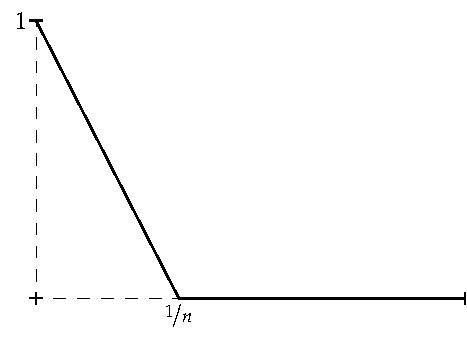
\includegraphics{figures/contconvcntr}
\caption{Graph of $f_n(x)$.%
\label{contconvcntr:fig}}
\end{myfigureht}

Each function $f_n$ is continuous.
Fix an $x \in (0,1]$.  If $n \geq \nicefrac{1}{x}$,
then $x \geq \nicefrac{1}{n}$.  Therefore for $n \geq \nicefrac{1}{x}$,
we have $f_n(x) = 0$, and so
\begin{equation*}
\lim_{n \to \infty} f_n(x) = 0.
\end{equation*}
On the other hand if $x=0$, then
\begin{equation*}
\lim_{n \to \infty} f_n(0) = 
\lim_{n \to \infty} 1 = 1.
\end{equation*}
Thus the pointwise limit of $f_n$ is the function
$f \colon [0,1] \to \R$ defined by
\begin{equation*}
f(x) :=
\begin{cases}
1 &  \text{if } x = 0,\\
0 &  \text{if } x > 0.
\end{cases}
\end{equation*}
The function $f$ is not continuous at 0.
\end{example}

If we, however, require the convergence to be uniform, the limits can
be interchanged.

\begin{thm}
Let $\{ f_n \}$ be 
a sequence of continuous functions $f_n \colon S \to \R$ converging
uniformly to  $f \colon S \to \R$.  Then $f$ is continuous.
\end{thm}

\begin{proof}
Let $x \in S$ be fixed.  Let $\{ x_n \}$ be a sequence in $S$
converging to $x$.

Let $\epsilon > 0$ be given.
As $\{ f_k \}$ converges uniformly to $f$, we find a $k \in \N$ such that
\begin{equation*}
\abs{f_k(y)-f(y)} < \nicefrac{\epsilon}{3}
\end{equation*}
for all $y \in S$.  As $f_k$ is continuous at $x$,
we find an $N \in \N$ such that for all $m \geq N$,
\begin{equation*}
\abs{f_k(x_m)-f_k(x)} < \nicefrac{\epsilon}{3} .
\end{equation*}
Thus for all
$m \geq N$,
\begin{equation*}
\begin{split}
\abs{f(x_m)-f(x)}
& =
\abs{f(x_m)-f_k(x_m)+f_k(x_m)-f_k(x)+f_k(x)-f(x)}
\\
& \leq
\abs{f(x_m)-f_k(x_m)}+
\abs{f_k(x_m)-f_k(x)}+
\abs{f_k(x)-f(x)}
\\
& <
\nicefrac{\epsilon}{3} +
\nicefrac{\epsilon}{3} +
\nicefrac{\epsilon}{3} = \epsilon .
\end{split}
\end{equation*}
Therefore $\bigl\{ f(x_m) \bigr\}$ converges to $f(x)$ and hence $f$ is continuous at
$x$.  As $x$ was arbitrary, $f$ is continuous everywhere.
\end{proof}

\subsection{Integral of the limit}

Again, if we simply require pointwise convergence, then the integral
of a limit of a sequence of functions need not be equal to the limit
of the integrals.

\begin{example}
Define $f_n \colon [0,1] \to \R$ as
\begin{equation*}
f_n(x) :=
\begin{cases}
0 &  \text{if } x = 0,\\
n-n^2x &  \text{if } 0 < x < \nicefrac{1}{n},\\
0 &  \text{if } x \geq \nicefrac{1}{n}.
\end{cases}
\end{equation*}
See \figureref{intconvcntr:fig}.

\begin{myfigureht}
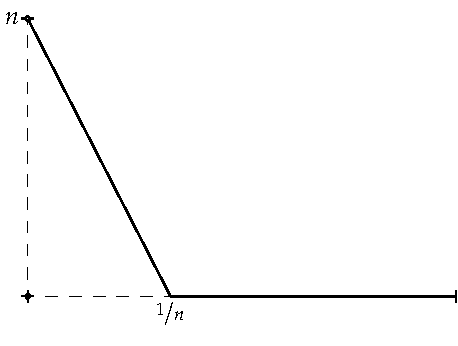
\includegraphics{figures/intconvcntr}
\caption{Graph of $f_n(x)$.%
\label{intconvcntr:fig}}
\end{myfigureht}

Each $f_n$ is Riemann integrable (it is continuous on $(0,1]$ and bounded),
and it is easy to see
\begin{equation*}
\int_0^1 f_n =
\int_0^{\nicefrac{1}{n}} (n-n^2x)~dx = \nicefrac{1}{2} .
\end{equation*}
Let us compute the pointwise limit of $\{ f_n \}$.
Fix an $x \in (0,1]$.  For $n \geq \nicefrac{1}{x}$,
we have $x \geq \nicefrac{1}{n}$ and so $f_n(x) = 0$.  Therefore,
\begin{equation*}
\lim_{n \to \infty} f_n(x) = 0.
\end{equation*}
We also have $f_n(0) = 0$ for all $n$.  Therefore the pointwise
limit of $\{ f_n \}$ is the zero function.  Thus
\begin{equation*}
\nicefrac{1}{2} =
\lim_{n\to\infty}
\int_0^1 f_n (x)~dx
\not=
\int_0^1
\left(
\lim_{n\to\infty}
f_n(x)\right)~dx
=
\int_0^1 0~dx = 0 .
\end{equation*}
\end{example}

But
if we again require the convergence to be uniform, the limits can
be interchanged.

\begin{thm} \label{integralinterchange:thm}
Let $\{ f_n \}$ be a sequence of Riemann integrable
functions
$f_n \colon [a,b] \to \R$
converging uniformly to $f \colon [a,b]
\to \R$.  Then $f$ is Riemann integrable, and
\begin{equation*}
\int_a^b f = \lim_{n\to\infty} \int_a^b f_n .
\end{equation*}
\end{thm}

\begin{proof}
Let $\epsilon > 0$ be given.
As $f_n$ goes to $f$ uniformly, we find an $M \in \N$ such that
for all $n \geq M$, we have 
$\abs{f_n(x)-f(x)} < \frac{\epsilon}{2(b-a)}$ for all $x \in [a,b]$.
In particular, by reverse triangle inequality,
$\abs{f(x)} < \frac{\epsilon}{2(b-a)} + \abs{f_n(x)}$ for all $x$.
Hence $f$ is bounded,
as $f_n$ is bounded.
Note that $f_n$ is integrable and compute
\begin{equation*}
\begin{split}
\overline{\int_a^b} f
-
\underline{\int_a^b} f
& =
\overline{\int_a^b} \bigl( f(x) - f_n(x) + f_n(x) \bigr)~dx
-
\underline{\int_a^b} \bigl( f(x) - f_n(x) + f_n(x) \bigr)~dx
\\
& \leq
\overline{\int_a^b} \bigl( f(x) - f_n(x) \bigr)~dx +  \overline{\int_a^b} f_n(x) ~dx
-
\underline{\int_a^b} \bigl( f(x) - f_n(x) \bigr)~dx -  \underline{\int_a^b} f_n(x) ~dx
\\
& =
\overline{\int_a^b} \bigl( f(x) - f_n(x) \bigr)~dx +  \int_a^b f_n(x) ~dx
-
\underline{\int_a^b} \bigl( f(x) - f_n(x) \bigr)~dx -  \int_a^b f_n(x) ~dx
\\
& =
\overline{\int_a^b} \bigl( f(x) - f_n(x) \bigr)~dx
-
\underline{\int_a^b} \bigl( f(x) - f_n(x) \bigr)~dx
\\
& \leq
\frac{\epsilon}{2(b-a)} (b-a) + 
\frac{\epsilon}{2(b-a)} (b-a) = \epsilon .
\end{split}
\end{equation*}
The first inequality is \propref{prop:upperlowerlinineq}.
The second inequality follows from \propref{intulbound:prop} and 
the fact that for all $x \in [a,b]$, we have
$\frac{-\epsilon}{2(b-a)} < f(x)-f_n(x) < \frac{\epsilon}{2(b-a)}$.
As $\epsilon > 0$ was arbitrary, $f$ is Riemann integrable.

Finally we compute $\int_a^b f$.  We apply \propref{intbound:prop}
in the calculation.  Again, for all $n \geq M$ (where $M$ is the same as above),
\begin{equation*}
\begin{split}
\abs{\int_a^b f - \int_a^b f_n} & = 
\abs{ \int_a^b \bigl(f(x) - f_n(x)\bigr)~dx}
\\
& \leq
\frac{\epsilon}{2(b-a)} (b-a) = \frac{\epsilon}{2} < \epsilon .
\end{split}
\end{equation*}
Therefore, $\{ \int_a^b f_n \}$ converges to $\int_a^b f$.
\end{proof}

\begin{example}
Suppose we wish to compute
\begin{equation*}
\lim_{n\to\infty} \int_0^1 \frac{nx+ \sin(nx^2)}{n} ~dx .
\end{equation*}
It is impossible to compute the integrals for any particular $n$ using 
calculus as $\sin(nx^2)$ has no closed-form antiderivative.  However,
we can compute the limit.
We have shown before that $\frac{nx+ \sin(nx^2)}{n}$ converges uniformly
on $[0,1]$ to $x$.
By \thmref{integralinterchange:thm}, the limit exists and
\begin{equation*}
\lim_{n\to\infty} \int_0^1 \frac{nx+ \sin(nx^2)}{n} ~dx
=
\int_0^1
x ~dx = \nicefrac{1}{2} .
\end{equation*}
\end{example}

\begin{example}
If convergence is only pointwise, the limit need not even be Riemann
integrable.  On $[0,1]$ define
\begin{equation*}
f_n(x) :=
\begin{cases}
1 & \text{if } x = \nicefrac{p}{q} \text{ in lowest terms and } q \leq n, \\
0 & \text{otherwise.}
\end{cases}
\end{equation*}
The function $f_n$ differs from the zero function at finitely many points;
there are only finitely many fractions in $[0,1]$ with denominator less than
or equal to $n$.   So $f_n$ is integrable and $\int_0^1 f_n = \int_0^1 0 =
0$.  It is an easy exercise to show that $\{ f_n \}$ converges pointwise to the
\myindex{Dirichlet function}
\begin{equation*}
f(x) :=
\begin{cases}
1 & \text{if } x \in \Q, \\
0 & \text{otherwise,}
\end{cases}
\end{equation*}
which is not Riemann integrable.
\end{example}

\begin{example}
In fact, if the convergence is only pointwise, the limit of bounded
functions is not even necessarily bounded.
Define $f_n \colon [0,1] \to \R$ by
\begin{equation*}
f_n(x) :=
\begin{cases}
0 & \text{if } x < \nicefrac{1}{n},\\
\nicefrac{1}{x} & \text{else.}
\end{cases}
\end{equation*}
For every $n$ we get that $\abs{f_n(x)} \leq n$ for all $x \in [0,1]$ so the
functions are bounded.  However $f_n$ converge pointwise to
\begin{equation*}
f(x) :=
\begin{cases}
0 & \text{if } x = 0,\\
\nicefrac{1}{x} & \text{else,}
\end{cases}
\end{equation*}
which is unbounded.
\end{example}

\subsection{Derivative of the limit}

While uniform convergence is enough to swap limits with integrals, it is not,
however, enough to swap limits with derivatives, unless you also have
uniform convergence of the derivatives themselves.

\begin{example}
Let $f_n(x) := \frac{\sin(nx)}{n}$.  Then $f_n$ converges uniformly to
0.  See \figureref{fig:conv1nsinxn}.
The derivative of the limit is 0.  But $f_n'(x) = \cos(nx)$, which
does not converge even pointwise, for
example $f_n'(\pi) = {(-1)}^n$.  Furthermore,
$f_n'(0) = 1$ for all $n$, which does converge, but not to $0$.
\begin{myfigureht}
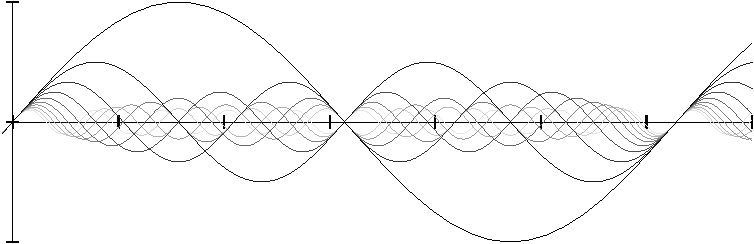
\includegraphics{figures/conv1nsinxn}
\caption{Graphs of $\frac{\sin(nx)}{n}$ for
$n=1,2,\ldots,10$, with higher $n$ in lighter gray.%
\label{fig:conv1nsinxn}}
\end{myfigureht}
\end{example}

\begin{example} \label{exercise:badconvergenceder}
Let $f_n(x) := \frac{1}{1+nx^2}$.
If $x \not= 0$, then $\lim_{n \to \infty} f_n(x) = 0$
and $\lim_{n \to \infty} f_n(0) = 1$.
Hence $\{ f_n \}$ converges pointwise to a function that is not continuous
at $0$.
We compute
\begin{equation*}
f_n'(x) %= \frac{d}{dx} \frac{1}{1+n x^2}
= \frac{-2 n x}{(1+ n x^2)^2} .
\end{equation*}
For every $x$, $\lim_{n\to\infty} f_n'(x) = 0$, so the derivatives
converge pointwise to 0,
but the reader can check that the convergence is not uniform on any closed
interval containing $0$.
The limit of $f_n$ is not differentiable at $0$, it is not even
continuous at $0$.
\end{example}

See the exercises for more examples.  Using 
the fundamental theorem of calculus we find an answer for continuously
differentiable functions.  The following theorem is true even if 
we do not assume continuity of the derivatives, but the proof is more
difficult.

\begin{thm} \label{thm:dersconverge}
Let $I$ be a bounded interval and let
$f_n \colon I \to \R$ be continuously differentiable functions.
Suppose $\{ f_n' \}$ converges uniformly to $g \colon I \to \R$,
and suppose $\bigl\{ f_n(c) \bigr\}_{n=1}^\infty$ is a
convergent sequence for some $c \in I$.  Then $\{ f_n \}$ converges uniformly to 
a continuously differentiable function $f \colon I \to \R$, and $f' = g$.
\end{thm}

\begin{proof}
Define $f(c) := \lim_{n\to \infty} f_n(c)$.
As $f_n'$ are continuous and hence Riemann integrable,
then
via the fundamental theorem of calculus, we find that for $x \in I$,
\begin{equation*}
f_n(x) = f_n(c) + \int_c^x f_n' .
\end{equation*}
As $\{ f_n' \}$ converges uniformly on $I$, it converges uniformly
on $[c,x]$ (or $[x,c]$ if $x < c$).
Therefore, we find that the limit on the right-hand side exists.
Let us define $f$ at the remaining points by this limit:
\begin{equation*}
f(x) :=
\lim_{n\to\infty} f_n(c) + \lim_{n\to\infty} \int_c^x f_n'
=
f(c) + \int_c^x g .
\end{equation*}
The function $g$ is continuous, being the uniform limit of continuous
functions.  Hence $f$ is differentiable and $f'(x) = g(x)$ for all $x \in I$
by the second form of the fundamental theorem.

It remains to prove
uniform convergence.
Suppose $I$ has a lower bound $a$ and upper bound $b$.
Let $\epsilon > 0$ be given.  Take $M$
such that for all $n \geq M$, we have
$\abs{f(c)-f_n(c)} < \nicefrac{\epsilon}{2}$,
and
$\abs{g(x)-f_n'(x)} < \nicefrac{\epsilon}{2(b-a)}$
for all $x \in I$.  Then
\begin{equation*}
\begin{split}
\abs{f(x) - f_n(x)} & =
\abs{f(c) + \int_c^x g - f_n(c) - \int_c^x f_n'}
\\
& \leq
\abs{f(c) - f_n(c)} + \abs{\int_c^x g - \int_c^x f_n'}
\\
& =
\abs{f(c) - f_n(c)} + \abs{\int_c^x \bigl(g(s) - f_n'(s)\bigr) \, ds}
\\
& <
\frac{\epsilon}{2}
+
\frac{\epsilon}{2(b-a)}
(b-a)
=\epsilon. \qedhere
\end{split}
\end{equation*}
\end{proof}

The proof goes through without boundedness of $I$, except for the
uniform convergence of $f_n$ to $f$.  As an example suppose $I = \R$ and let
$f_n(x) := \nicefrac{x}{n}$.  Then $f_n'(x)=\nicefrac{1}{n}$, which
converges uniformly to $0$.  However, $\{f_n\}$ converges to 0 only pointwise.

\subsection{Convergence of power series}

In \sectionref{sec:moreonseries} we saw that a power series converges
absolutely inside its radius of convergence, so it converges pointwise.
Let us show that it (and all its derivatives) also converges uniformly.
This fact allows us to
swap several types of limits.  Not only is the limit continuous,
we can
integrate and even differentiate convergent power series term by term.

\begin{prop}
Let $\sum_{n=0}^\infty c_n {(x-a)}^n$ be a convergent power series with a radius
of convergence $\rho$, where $0 < \rho \leq \infty$.
Then the series converges uniformly
in $[a-r,a+r]$ whenever $0 < r < \rho$.

In particular, the series defines a continuous function
on $(a-\rho,a+\rho)$ (if $\rho < \infty$), or $\R$ (if $\rho = \infty$).
\end{prop}

\begin{proof}
Let $I := (a-\rho,a+\rho)$ if $\rho < \infty$,
or let $I := \R$ if $\rho= \infty$.
Take $0 < r < \rho$.
The series converges absolutely for every $x \in I$,
in particular if $x = a+r$.
Therefore $\sum_{n=0}^\infty \abs{c_n} r^n$ converges.
Given $\epsilon >0$, find $M$ such that for all $k \geq M$,
\begin{equation*}
\sum_{n=k+1}^\infty \abs{c_n} {r}^n < \epsilon .
\end{equation*}
For all $x \in [a-r,a+r]$ and all $m > k$,
\begin{multline*}
\abs{\sum_{n=0}^m c_n {(x-a)}^n - 
\sum_{n=0}^k c_n {(x-a)}^n}
=
\abs{\sum_{n=k+1}^m c_n {(x-a)}^n}
\\
\leq
\sum_{n=k+1}^m \abs{c_n} {\abs{x-a}}^n
\leq
\sum_{n=k+1}^m \abs{c_n} {r}^n
\leq
\sum_{n=k+1}^\infty \abs{c_n} {r}^n
<\epsilon.
\end{multline*}
The partial sums are therefore uniformly Cauchy on $[a-r,a+r]$ and
hence converge uniformly on that set.

Moreover, the partial sums are polynomials, which are
continuous, and so their uniform limit on $[a-r,a+r]$
is a continuous function.
As $r < \rho$ was arbitrary, the limit function
is continuous on all of $I$.
\end{proof}

As we said, we will show that
power series can be differentiated and integrated
term by term.  The 
differentiated or integrated series is again a power series,
and we will show it has the same radius of convergence.
Therefore, 
any power series defines an infinitely differentiable function.

We first prove that we can antidifferentiate, as integration only needs
uniform limits.

\begin{cor}
Let $\sum_{n=0}^\infty c_n {(x-a)}^n$ be a convergent power series with a radius
of convergence $0 < \rho \leq \infty$.
Let $I := (a-\rho,a+\rho)$ if $\rho < \infty$
or $I := \R$ if $\rho= \infty$.  Let $f \colon I \to \R$ be the limit.
Then
\begin{equation*}
\int_a^x f = \sum_{n=1}^\infty \frac{c_{n-1}}{n} {(x-a)}^{n} ,
\end{equation*}
where the radius of convergence of this series is at least $\rho$.
\end{cor}

\begin{proof}
Take $0 < r < \rho$.
The partial sums $\sum_{n=0}^k c_n {(x-a)}^n$ converge uniformly on $[a-r,a+r]$.
For every fixed $x \in [a-r,a+r]$, the convergence is also uniform
on $[a,x]$ (or $[x,a]$ if $x < a$).
Hence,
\begin{equation*}
\int_a^x f =
\int_a^x \lim_{k\to\infty} \sum_{n=0}^k c_n {(s-a)}^n \, ds
=
\lim_{k\to\infty}
\int_a^x \sum_{n=0}^k c_n {(s-a)}^n \, ds
=
\lim_{k\to\infty}
\sum_{n=1}^{k+1} \frac{c_{n-1}}{n} {(x-a)}^{n} . \qedhere
\end{equation*}
\end{proof}


\begin{cor} \label{cor:differentiatepowerser}
Let $\sum_{n=0}^\infty c_n {(x-a)}^n$ be a convergent power series with a radius
of convergence $0 < \rho \leq \infty$.
Let $I := (a-\rho,a+\rho)$ if $\rho < \infty$
or $I := \R$ if $\rho= \infty$.  Let $f \colon I \to \R$ be the limit.
Then $f$ is a differentiable function, and
\begin{equation*}
f'(x) = \sum_{n=0}^\infty (n+1) c_{n+1} {(x-a)}^{n} ,
\end{equation*}
where the radius of convergence of this series is $\rho$.
\end{cor}

\begin{proof}
Take $0 < r < \rho$.
The series converges uniformly on
$[a-r,a+r]$,
but we need uniform convergence of the derivative.
Let
\begin{equation*}
R := \limsup_{n \to \infty} \abs{c_n}^{1/n} .
\end{equation*}
As the series is convergent $R < \infty$, and
the radius of convergence is $\nicefrac{1}{R}$ (or $\infty$ if $R=0$).

Let $\epsilon > 0$ be given.  In \exampleref{example:nto1overn} 
we saw $\lim\,n^{1/n} = 1$.
Hence there exists an $N$ such that for all $n \geq N$, we have
$n^{1/n} < 1+\epsilon$.

So
\begin{equation*}
R = 
\limsup_{n \to \infty}
\abs{c_n}^{1/n}
\leq
\limsup_{n \to \infty}
\abs{n c_n}^{1/n}
\leq
(1+\epsilon)
\limsup_{n \to \infty}
\abs{c_n}^{1/n}
=
(1+\epsilon)R .
\end{equation*}
As $\epsilon$ was arbitrary, $\limsup_{n \to \infty} \abs{n c_n}^{1/n} = R$.
Therefore, $\sum_{n=1}^\infty n c_{n} {(x-a)}^{n}$ has radius of
convergence $\rho$, and by dividing by $(x-a)$ we find
$\sum_{n=0}^\infty (n+1) c_{n+1} {(x-a)}^{n}$ has radius of convergence
$\rho$ as well.

Consequently, the partial sums 
$\sum_{n=0}^k (n+1) c_{n+1} {(x-a)}^{n}$,
which are derivatives of the partial sums
$\sum_{n=0}^{k+1} c_{n} {(x-a)}^{n}$,
converge uniformly on $[a-r,a+r]$.  Furthermore,
the series clearly converges at $x=a$.
We may thus apply \thmref{thm:dersconverge}, and
we are done as $r < \rho$ was arbitrary.
\end{proof}

\begin{example} \label{example:exponentialbypowerseries}
We could have used this result to define the exponential function.  That is,
the power series
\begin{equation*}
f(x) := \sum_{n=0}^\infty \frac{x^n}{n!}
\end{equation*}
has radius of convergence $\rho=\infty$.  Furthermore,
$f(0) = 1$, and by differentiating
term by term we find that $f'(x) = f(x)$.
\end{example}

\begin{example}
The series
\begin{equation*}
\sum_{n=1}^\infty n x^n
\end{equation*}
converges to $\frac{x}{{(1-x)}^2}$ on $(-1,1)$.

Proof:
On $(-1,1)$, $\sum_{n=0}^\infty x^n$ converges to
$\frac{1}{1-x}$.  The derivative $\sum_{n=1}^\infty n x^{n-1}$ then converges
on the same interval to $\frac{1}{{(1-x)}^2}$.  Multiplying by $x$
obtains the result.
\end{example}

\subsection{Exercises}

\begin{exercise}
While uniform convergence preserves continuity, it does not preserve
differentiability.  Find an explicit example of a sequence of
differentiable functions on $[-1,1]$ that converge uniformly to
a function $f$ such that $f$ is not differentiable.
Hint:
There are many possibilities,
simplest is perhaps to combine $\abs{x}$ and $\frac{n}{2}x^2 +
\frac{1}{2n}$, another is to
consider $\sqrt{x^2+{(\nicefrac{1}{n})}^2}$.  Show that these functions are differentiable,
converge uniformly, and then show that the limit is not differentiable.
\end{exercise}

\begin{exercise}
Let $f_n(x) := \frac{x^n}{n}$.  Show that $\{ f_n \}$ converges uniformly to
a differentiable function $f$ on $[0,1]$ (find $f$).  However, show that
$f'(1) \not= \lim\limits_{n\to\infty} f_n'(1)$.
\end{exercise}

\begin{exnote}
Note: The previous two exercises show that
we cannot simply swap limits with derivatives, even if the convergence is
uniform.  See also \exerciseref{c1uniflim:exercise} below.
\end{exnote}

\begin{exercise}
Let $f \colon [0,1] \to \R$ be a Riemann integrable (hence bounded)
function.  Find
$\displaystyle \lim_{n\to\infty} \int_0^1 \frac{f(x)}{n} ~dx$.
\end{exercise}

\begin{exercise}
Show
$\displaystyle \lim_{n\to\infty} \int_1^2 e^{-nx^2} ~dx = 0$.  Feel free to
use
what you know about the exponential function from calculus.
\end{exercise}

\begin{exercise}
Find an example of a sequence of continuous functions on $(0,1)$ that converges 
pointwise to a continuous function on $(0,1)$, but the convergence is not
uniform.
\end{exercise}

\begin{exnote}
Note: In the previous exercise, $(0,1)$ was picked for simplicity.  For a
more challenging exercise, replace $(0,1)$ with $[0,1]$.
\end{exnote}

\begin{exercise}
True/False; prove or find a counterexample to the following statement:
If $\{ f_n \}$ is a sequence of everywhere discontinuous functions on $[0,1]$
that converge uniformly to a function $f$, then $f$ is everywhere
discontinuous.
\end{exercise}

\begin{exercise} \label{c1uniflim:exercise}
For a continuously differentiable function $f \colon [a,b] \to \R$, define
\begin{equation*}
\norm{f}_{C^1} := \norm{f}_u + \norm{f'}_u .
\end{equation*}
Suppose $\{ f_n \}$ is a sequence of continuously differentiable
functions such that for every $\epsilon >0$, there exists an $M$
such that for all $n,k \geq M$, we have
\begin{equation*}
\norm{f_n-f_k}_{C^1} < \epsilon .
\end{equation*}
Show that $\{ f_n \}$ converges uniformly to some continuously differentiable
function $f \colon [a,b] \to \R$.
\end{exercise}

\begin{exnote}
Suppose 
$f \colon [0,1] \to \R$ is Riemann integrable.
For the following two exercises define 
the number
\begin{equation*}
\norm{f}_{L^1} := 
\int_0^1 \abs{f(x)}~dx .
\end{equation*}
It is true that $\abs{f}$ is integrable whenever $f$ is, see
\exerciseref{exercise:hardabsint}.
The number is called the \emph{$L^1$-norm}\index{L1-norm@$L^1$-norm} and
defines another very common type of
convergence called the
\emph{$L^1$-convergence}\index{L1-convergence@$L^1$-convergence}.
It is, however, a bit more subtle.
\end{exnote}

\begin{exercise}
Suppose $\{ f_n \}$ is a sequence of Riemann integrable functions on $[0,1]$
that converges uniformly
to $0$.  Show that
\begin{equation*}
\lim_{n\to\infty} \norm{f_n}_{L^1} = 0 .
\end{equation*}
\end{exercise}

\begin{exercise}
Find a sequence $\{ f_n \}$ of Riemann integrable functions 
on $[0,1]$ converging pointwise to $0$, but
\begin{equation*}
\lim_{n\to\infty} \norm{f_n}_{L^1} \text{ does not exist (is } \infty\text{)}.
\end{equation*}
\end{exercise}

\begin{exercise}[Hard] \label{exercise:dinisthm}
Prove \emph{\myindex{Dini's theorem}}:
Let $f_n \colon [a,b] \to \R$ be a sequence of continuous functions such that
\begin{equation*}
0 \leq f_{n+1}(x) \leq f_n(x) \leq \cdots \leq f_1(x) 
\qquad \text{for all } n \in \N.
\end{equation*}
Suppose $\{ f_n \}$ converges pointwise to $0$.
Show that $\{ f_n \}$ converges to zero uniformly.
\end{exercise}

\begin{exercise}
Suppose $f_n \colon [a,b] \to \R$ is a sequence of continuous
functions that
converges pointwise
to a continuous $f \colon [a,b] \to \R$.  Suppose that
for every $x \in [a,b]$, the sequence $\{ \abs{f_n(x)-f(x)} \}$ is monotone.
Show that the sequence $\{f_n\}$ converges uniformly.
\end{exercise}

\begin{exercise}
Find a sequence of Riemann integrable functions $f_n \colon [0,1] \to \R$ such
that $\{ f_n \}$ converges to zero pointwise, and such that
\begin{enumerate}[a)]
\item
$\bigl\{ \int_0^1 f_n \bigr\}_{n=1}^\infty$ increases without bound,
\item
$\bigl\{ \int_0^1 f_n \bigr\}_{n=1}^\infty$ is the sequence $-1,1,-1,1,-1,1, \ldots$.
\end{enumerate}
\end{exercise}

\begin{exnote}
It is possible to define a 
\emph{\myindex{joint limit}} of a double sequence $\{ x_{n,m} \}$ of real
numbers (that is a function from $\N \times \N$ to $\R$).
We say $L$ is the joint limit of $\{ x_{n,m} \}$ and write
\begin{equation*}
\lim_{\substack{n\to\infty\\m\to\infty}}
x_{n,m} = L ,
\qquad
\text{or}
\qquad
\lim_{(n,m) \to \infty}
x_{n,m} = L ,
\end{equation*}
if for every $\epsilon > 0$, there
exists an $M$ such that if $n \geq M$ and $m \geq M$, then
$\abs{x_{n,m} - L} < \epsilon$.
\end{exnote}

\begin{exercise}
Suppose the joint limit (see above) of $\{ x_{n,m} \}$ is $L$, and suppose
that for all $n$, $\lim\limits_{m \to \infty} x_{n,m}$ exists,
and for all $m$, $\lim\limits_{n \to \infty} x_{n,m}$ exists.  Then show
$\lim\limits_{n\to\infty}\lim\limits_{m \to \infty} x_{n,m}
=
\lim\limits_{m\to\infty}\lim\limits_{n \to \infty} x_{n,m} = L$.
\end{exercise}

\begin{exercise}
A joint limit (see above) does not mean the iterated limits even exist.
Consider $x_{n,m} := \frac{{(-1)}^{n+m}}{\min \{n,m \}}$.
\begin{enumerate}[a)]
\item
Show that for no $n$ does
$\lim\limits_{m \to \infty} x_{n,m}$ exist, and for no $m$
does 
$\lim\limits_{n \to \infty} x_{n,m}$ exist.  So neither
$\lim\limits_{n\to\infty}\lim\limits_{m \to \infty} x_{n,m}$ nor
$\lim\limits_{m\to\infty}\lim\limits_{n \to \infty} x_{n,m}$ makes any sense
at all.
\item
Show that the joint limit of $\{ x_{n,m} \}$ exists and equals 0.
\end{enumerate}
\end{exercise}

\begin{exercise}
We say that a sequence of functions $f_n \colon \R \to \R$
\emph{\myindex{converges uniformly on compact subsets}}
\index{uniform convergence on compact subsets}
if for every $k \in \N$,
the sequence $\{ f_n \}$ converges uniformly on $[-k,k]$.
\begin{enumerate}[a)]
\item
Prove that if $f_n \colon \R \to \R$ is a sequence of
continuous functions converging uniformly on compact subsets, then
the limit is continuous.
\item 
Prove that if $f_n \colon \R \to \R$ is a sequence of
functions Riemann integrable on every closed and bounded interval $[a,b]$,
and converging uniformly on compact subsets to an $f \colon \R \to \R$,
then for every interval $[a,b]$, we have $f \in \sR[a,b]$, and
$\int_a^b f = \lim_{n\to\infty} \int_a^b f_n$.
\end{enumerate}
\end{exercise}

\begin{exercise}[Challenging]
Find a sequence of continuous functions $f_n \colon [0,1] \to \R$ that
converge to the popcorn function $f \colon [0,1] \to \R$, that is the
function such that $f(\nicefrac{p}{q}) := \frac{1}{q}$ (if $\nicefrac{p}{q}$
is in lowest terms) and $f(x) := 0$ if $x$ is not rational (note
that $f(0) = f(1) = 1$),
see \exampleref{popcornfunction:example}.
So a pointwise limit of continuous functions can have a dense set of
discontinuities.  See also the next exercise.
\end{exercise}

\begin{exercise}[Challenging]
The \myindex{Dirichlet function}
$f \colon [0,1] \to \R$, that is the
function such that $f(x) := 1$ if $x \in \Q$
and $f(x) := 0$ if $x \notin \Q$,
is not the pointwise limit of
continuous functions, although this is difficult to show.
Prove, however, that $f$ is a pointwise limit of functions that are themselves
pointwise limits of
continuous functions themselves.
\end{exercise}

\begin{exercise}
\leavevmode
\begin{enumerate}[a)]
\item
Find a sequence of Lipschitz continuous functions on $[0,1]$
whose uniform limit is $\sqrt{x}$, which is a non-Lipschitz function.
\item
On the other hand, show that if $f_n \colon S \to \R$ are Lipschitz
with a uniform constant $K$ (meaning all of them satisfy the definition
with the same constant) and $\{ f_n \}$ converges pointwise
to $f \colon S \to \R$,
then the limit $f$ is a Lipschitz continuous function
with Lipschitz constant $K$.
\end{enumerate}
\end{exercise}

\begin{exercise}[requires \sectionref{sec:moreonseries}]
If $\sum_{n=0}^\infty c_n {(x-a)}^n$ has radius of convergence $\rho$,
show that the term by term integral
$\sum_{n=1}^\infty \frac{c_{n-1}}{n} {(x-a)}^n$ has radius of convergence
$\rho$.  Note that we only proved above that the radius of convergence was
at least $\rho$.
\end{exercise}

\begin{exercise}[requires \sectionref{sec:moreonseries} and \sectionref{sec:taylor}]
Suppose $f(x) := \sum_{n=0}^\infty c_n {(x-a)}^n$ converges in $(a-\rho,a+\rho)$.
\begin{enumerate}[a)]
\item
Suppose that $f^{(k)}(a) = 0$ for all $k=0,1,2,3,\ldots$.  Prove that
$c_n = 0$ for all $n$, or in other words, 
$f(x) = 0$ for all $x \in (a-\rho,a+\rho)$.
\item
Using part a) prove a version of the so-called \myquote{identity
theorem for analytic functions}:  If there exists an $\epsilon > 0$
such that $f(x) = 0$ for all $x \in (a-\epsilon, a+\epsilon)$, then
$f(x) = 0$ for all $x \in (a-\rho,a+\rho)$.
\end{enumerate}
\end{exercise}

\begin{exercise}
Let $f_n(x) := \frac{x}{1+{(nx)}^2}$.  Notice that $f_n$ are differentiable
functions.
\begin{enumerate}[a)]
\item
Show that $\{ f_n \}$ converges uniformly to 0.
\item
Show that $\sabs{f_n'(x)} \leq 1$ for all $x$ and all $n$.
\item
Show that $\{ f_n' \}$ converges pointwise to a function discontinuous at
the origin.
\item
Let $\{ a_n \}$ be an enumeration of the rational numbers.
Define
\begin{equation*}
g_n(x) := \sum_{k=1}^n 2^{-k} f_n(x-a_k) .
\end{equation*}
Show that $\{ g_n \}$ converges uniformly to 0.
\item
Show that $\{ g_n' \}$ converges pointwise to a function $\psi$ that
is discontinuous at every rational number and continuous at every
irrational number.  In particular, $\lim_{n\to\infty} g_n'(x) \not= 0$ for
every rational number $x$.
\end{enumerate}
\end{exercise}

%%%%%%%%%%%%%%%%%%%%%%%%%%%%%%%%%%%%%%%%%%%%%%%%%%%%%%%%%%%%%%%%%%%%%%%%%%%%%%

\sectionnewpage
\section{Picard's theorem}
\label{sec:picard}

\sectionnotes{1--2 lectures (can be safely skipped)}

A first semester course in analysis should have
a \emph{pi\`ece de r\'esistance} caliber
theorem.  We pick a theorem whose proof combines everything we have
learned.  It is more sophisticated than the fundamental theorem of calculus,
the first highlight theorem of this course.  The
theorem we are talking about is Picard's
theorem%
\footnote{Named for the French mathematician
\href{https://en.wikipedia.org/wiki/\%C3\%89mile_Picard}{Charles \'Emile Picard}
(1856--1941).}
on existence and uniqueness of a solution to an ordinary differential equation.
Both the statement and the proof are beautiful examples of what one can do
with the material we mastered so far.  It is also a good example of how analysis is
applied as differential equations are indispensable in science of every
stripe.

\subsection{First order ordinary differential equation}

Modern science is described in the language of
\emph{differential equations}\index{differential equation}.
That is, equations involving not only the unknown, but also its
derivatives.  The simplest nontrivial form of a differential equation is
the so-called \emph{\myindex{first order ordinary differential equation}}
\index{ordinary differential equation}
\begin{equation*}
y' = F(x,y) .
\end{equation*}
Generally we also specify an \emph{\myindex{initial condition}}
$y(x_0)=y_0$.  The solution of
the equation is a function $y(x)$ such that 
$y(x_0)=y_0$ and $y'(x) = F\bigl(x,y(x)\bigr)$.

When $F$ involves only the $x$ variable, the solution is given by the
fundamental theorem of calculus.  On the other hand, when $F$ depends
on both $x$ and $y$ we need far more firepower.  It is not always
true that a solution exists, and if it does, that it is the unique solution.
Picard's theorem gives us certain sufficient conditions for existence
and uniqueness.

\subsection{The theorem}

We need a definition of continuity in two variables.  A point in the
plane $\R^2 = \R \times \R$ is denoted by an ordered pair $(x,y)$.
For simplicity,
we give the following sequential definition of continuity.

\begin{defn}
Let $U \subset \R^2$ be a set, $F \colon U \to \R$ a function,
and $(x,y) \in U$ a point.  The function $F$ is \emph{continuous}
\index{continuous function of two variables}
at $(x,y)$ if 
for every sequence
$\bigl\{ (x_n,y_n) \bigr\}_{n=1}^\infty$ of points in $U$ such that
$\lim\, x_n = x$ and 
$\lim\, y_n = y$, we have 
\begin{equation*}
\lim_{n \to \infty} F(x_n,y_n) = 
F(x,y) .
\end{equation*}
We say $F$ is continuous if it is continuous at all points in $U$.
\end{defn}

\begin{thm}[Picard's theorem on existence and uniqueness]%
\index{existence and uniqueness theorem}\index{Picard's theorem}%
\label{thm:fs:picard}
Let $I, J \subset \R$ be closed bounded intervals, 
let $I^\circ$ and $J^\circ$ be their interiors%
\footnote{By interior of $[a,b]$ we mean $(a,b)$.},
and
let $(x_0,y_0) \in I^\circ \times J^\circ$.
Suppose $F \colon I \times J \to \R$ is continuous
and Lipschitz in the second variable, that is, there exists
an $L \in \R$ such that
\begin{equation*}
\abs{F(x,y) - F(x,z)} \leq L \abs{y-z}
\qquad \text{for all } y,z \in J, x \in I .
\end{equation*}
Then there exists an $h > 0$ and a unique differentiable
function $f \colon [x_0 - h, x_0 + h] \to J \subset \R$, such that
\begin{equation} \label{picard:diffeq}
f'(x) = F\bigl(x,f(x)\bigr) \qquad \text{and} \qquad f(x_0) = y_0.
\pagebreak[2]
\end{equation}
\end{thm}

\begin{proof}
Suppose we could find a solution $f$.  Using the fundamental
theorem of calculus we integrate the equation 
$f'(x) = F\bigl(x,f(x)\bigr)$, $f(x_0) = y_0$, and write \eqref{picard:diffeq}
as the integral equation
\begin{equation} \label{picard:inteq}
f(x) = y_0 + \int_{x_0}^x F\bigl(t,f(t)\bigr)~dt .
\end{equation}
The idea of our proof is that we try to plug in approximations to
a solution to the right-hand side of \eqref{picard:inteq} to get better approximations on the
left-hand side of  \eqref{picard:inteq}.  We hope that in the end the sequence 
converges and solves
\eqref{picard:inteq} and hence \eqref{picard:diffeq}.
The technique below is called \emph{\myindex{Picard iteration}},
and the individual functions $f_k$ are called the 
\emph{Picard iterates}\index{Picard iterate}.

Without loss of generality, suppose $x_0 = 0$ (exercise below).
Another
exercise tells us that $F$ is bounded as it is continuous.
Therefore pick some $M > 0$ so that 
$\abs{F(x,y)} \leq M$ for all $(x,y) \in I\times J$.
Pick $\alpha > 0$ such that
$[-\alpha,\alpha] \subset I$ and $[y_0-\alpha, y_0 + \alpha] \subset J$.
Define
\begin{equation*}
h := \min \left\{ \alpha, \frac{\alpha}{M+L\alpha} \right\} .
\end{equation*}
Observe
$[-h,h] \subset I$.

Set $f_0(x) := y_0$.
We define $f_k$ inductively.
Assuming $f_{k-1}([-h,h]) \subset [y_0-\alpha,y_0+\alpha]$,
we see 
$F\bigl(t,f_{k-1}(t)\bigr)$ is
a well-defined function of $t$ for $t \in [-h,h]$.
Further if $f_{k-1}$ is continuous
on $[-h,h]$, then
$F\bigl(t,f_{k-1}(t)\bigr)$ is
continuous as
a function of $t$ on $[-h,h]$ (left as an exercise).
Define
\begin{equation*}
f_k(x) := y_0+ \int_{0}^x F\bigl(t,f_{k-1}(t)\bigr)~dt ,
\end{equation*}
and $f_k$ is continuous on $[-h,h]$ by the fundamental theorem of calculus.
To see that $f_k$ maps $[-h,h]$ to $[y_0-\alpha,y_0+\alpha]$, we compute for
$x \in [-h,h]$
\begin{equation*}
\abs{f_k(x) - y_0} = 
\abs{\int_{0}^x F\bigl(t,f_{k-1}(t)\bigr)~dt }
\leq
M\abs{x}
\leq
Mh
\leq
M
\frac{\alpha}{M+L\alpha}
\leq \alpha .
\end{equation*}
We now define $f_{k+1}$ and so on, and
we have defined a sequence $\{ f_k \}$ of functions.  We need
to show that it converges to a function $f$ that solves
the equation \eqref{picard:inteq} and therefore \eqref{picard:diffeq}.

We wish to show that the sequence $\{ f_k \}$ converges uniformly
to some function on $[-h,h]$.  First, for $t \in [-h,h]$,
we have the following
useful bound
\begin{equation*}
\abs{F\bigl(t,f_{n}(t)\bigr) - 
F\bigl(t,f_{k}(t)\bigr)}
\leq
L \abs{f_n(t)-f_k(t)}
\leq
L \norm{f_n-f_k}_u ,
\end{equation*}
where $\norm{f_n-f_k}_u$ is the uniform norm, that
is the supremum of $\abs{f_n(t)-f_k(t)}$ for $t \in [-h,h]$.
Now note that $\abs{x} \leq h \leq \frac{\alpha}{M+L\alpha}$.
Therefore
\begin{equation*}
\begin{split}
\abs{f_n(x) - f_k(x)}
& =
\abs{\int_{0}^x F\bigl(t,f_{n-1}(t)\bigr)~dt 
-
\int_{0}^x F\bigl(t,f_{k-1}(t)\bigr)~dt}
\\
& =
\abs{\int_{0}^x F\bigl(t,f_{n-1}(t)\bigr)-
F\bigl(t,f_{k-1}(t)\bigr)~dt}
\\
& \leq
L\norm{f_{n-1}-f_{k-1}}_u
\abs{x}
\\
& \leq
\frac{L\alpha}{M+L\alpha}
\norm{f_{n-1}-f_{k-1}}_u .
\end{split}
\end{equation*}
Let $C := \frac{L\alpha}{M+L\alpha}$ and note that $C < 1$.
Taking supremum on the left-hand side we get
\begin{equation*}
\norm{f_n-f_k}_u \leq C \norm{f_{n-1}-f_{k-1}}_u .
\end{equation*}
Without loss of generality,
suppose $n \geq k$.  Then by \hyperref[induction:thm]{induction} we can show 
\begin{equation*}
\norm{f_n-f_k}_u \leq C^{k} \norm{f_{n-k}-f_{0}}_u .
\end{equation*}
For $x \in [-h,h]$, we have
\begin{equation*}
\abs{f_{n-k}(x)-f_{0}(x)}
=
\abs{f_{n-k}(x)-y_0}
\leq \alpha .
\end{equation*}
Therefore,
\begin{equation*}
\norm{f_n-f_k}_u \leq C^{k} \norm{f_{n-k}-f_{0}}_u \leq C^{k} \alpha .
\end{equation*}
As $C < 1$, $\{f_n\}$ is uniformly Cauchy and by
\propref{prop:uniformcauchy} we obtain that $\{ f_n \}$
converges uniformly on $[-h,h]$ to some function $f \colon [-h,h] \to \R$.
The function $f$ is the uniform limit of continuous functions and therefore
continuous.  Furthermore, since $f_n([-h,h]) \subset
[y_0-\alpha,y_0+\alpha]$ for all $n$, then $f([-h,h]) \subset [y_0-\alpha,y_0+\alpha]$
(why?).


We now need to show that $f$ solves \eqref{picard:inteq}.
First, as before we notice
\begin{equation*}
\abs{F\bigl(t,f_{n}(t)\bigr) - 
F\bigl(t,f(t)\bigr)}
\leq
L \abs{f_n(t)-f(t)}
\leq
L \norm{f_n-f}_u .
\end{equation*}
As $\norm{f_n-f}_u$ converges to 0, then
$F\bigl(t,f_n(t)\bigr)$ converges uniformly to $F\bigl(t,f(t)\bigr)$
for $t \in [-h,h]$.  Hence, for $x \in [-h,h]$
the convergence is uniform %(why?)
for $t \in [0,x]$ (or $[x,0]$ if $x < 0$).  Therefore,
\begin{align*}
y_0
+
\int_0^{x}
F(t,f(t)\bigr)~dt
& =
y_0
+
\int_0^{x}
F\bigl(t,\lim_{n\to\infty} f_n(t)\bigr)~dt
& &
\\
& =
y_0
+
\int_0^{x}
\lim_{n\to\infty} F\bigl(t,f_n(t)\bigr)~dt
& & \text{(by continuity of } F\text{)}
\\
& =
\lim_{n\to\infty} 
\left(
y_0
+
\int_0^{x}
F\bigl(t,f_n(t)\bigr)~dt
\right)
& & \text{(by uniform convergence)}
\\
& =
\lim_{n\to\infty} 
f_{n+1}(x)
=
f(x) .
& &
\end{align*}
We apply the fundamental theorem of calculus (\thmref{thm:FTCv2}) to show that
$f$ is differentiable and its derivative is $F\bigl(x,f(x)\bigr)$.  It is obvious
that $f(0) = y_0$.

Finally, what is left to do is to show uniqueness.  Suppose $g \colon [-h,h]
\to J \subset \R$ is another solution.
As before we use the fact that
$\abs{F\bigl(t,f(t)\bigr) - F\bigl(t,g(t)\bigr)} \leq L \norm{f-g}_u$.
Then
\begin{equation*}
\begin{split}
\abs{f(x)-g(x)}
& =
\abs{
y_0
+
\int_0^{x}
F\bigl(t,f(t)\bigr)~dt
-
\left(
y_0
+
\int_0^{x}
F\bigl(t,g(t)\bigr)~dt
\right)
}
\\
& =
\abs{
\int_0^{x}
F\bigl(t,f(t)\bigr)
-
F\bigl(t,g(t)\bigr)~dt
}
\\
& \leq
L\norm{f-g}_u\abs{x}
\leq
Lh\norm{f-g}_u
\leq
\frac{L\alpha}{M+L\alpha}\norm{f-g}_u .
\end{split}
\end{equation*}
As 
before, $C = \frac{L\alpha}{M+L\alpha} < 1$.  By taking supremum over $x \in
[-h,h]$ on the
left-hand side we obtain
\begin{equation*}
\norm{f-g}_u \leq C \norm{f-g}_u .
\end{equation*}
This is only possible if $\norm{f-g}_u = 0$.  Therefore, $f=g$, and the
solution is unique.
\end{proof}

\subsection{Examples}

Let us look at some examples.  The proof of the theorem 
gives us an explicit way to find an $h$ that works.  It does not, however, give
us the best $h$.  It is often possible to find a much larger $h$ for
which the conclusion of the theorem holds.

The proof also gives us the Picard iterates as approximations to the
solution.  So the proof actually tells us how to obtain
the solution, not just that the solution exists.

\begin{example} \label{example:picardexponential}
Consider
\begin{equation*}
f'(x) = f(x), \qquad f(0) = 1 .
\end{equation*}
That is, we suppose $F(x,y) = y$, and we are looking for a function 
$f$ such that $f'(x) = f(x)$.
Let us forget for the moment that we solved this equation in 
\sectionref{sec:logandexp}.

We pick any $I$ that contains 0
in the interior.
We pick an arbitrary $J$ that contains 1 in its interior.  We can
use $L = 1$.
The theorem guarantees an $h > 0$ such that
there exists a unique solution $f \colon [-h,h] \to \R$.  This solution
is usually denoted by
\begin{equation*}
e^x := f(x) .
\end{equation*}
We leave it to the reader to verify that by picking $I$ and $J$
large enough the proof of the theorem guarantees that
we are able to pick $\alpha$ such that we get any
$h$ we want as long as $h < \nicefrac{1}{2}$.  We omit the calculation.

Of course, we know %(though we have not proved)
this function exists
as a function for all $x$, so an arbitrary $h$ ought to work.
By same reasoning as above,
no matter what $x_0$ and $y_0$ are,
the proof guarantees an arbitrary $h$ as long as $h < \nicefrac{1}{2}$.
Fix such an $h$.
We get a unique function defined on $[x_0-h,x_0+h]$.  After defining the
function on $[-h,h]$ we find a solution on the interval $[0,2h]$
and notice that the two functions must coincide on $[0,h]$ by uniqueness.
We thus iteratively construct the exponential for all $x \in \R$.
Therefore Picard's theorem could be used to prove the existence and uniqueness
of the exponential.

Let us compute the Picard iterates.
We start with the constant function $f_0(x) := 1$.  Then
\begin{align*}
f_1(x) & = 1 + \int_0^x f_0(s)~ds =
1+x, \\
f_2(x) & = 1 + \int_0^x f_1(s)~ds =
1 + \int_0^x (1+s)~ds = 1 + x + \frac{x^2}{2}, \\
f_3(x) & = 1 + \int_0^x f_2(s)~ds =
1 + \int_0^x \left(1+ s + \frac{s^2}{2} \right)~ds =
1 + x + \frac{x^2}{2} + \frac{x^3}{6} .
\end{align*}
We recognize the beginning of the Taylor series for the exponential.
\end{example}

\begin{example}
Consider the equation
\begin{equation*}
f'(x) = {\bigl(f(x)\bigr)}^2 \qquad \text{and} \qquad f(0)=1.
\end{equation*}
From elementary differential equations we know 
\begin{equation*}
f(x) = \frac{1}{1-x}
\end{equation*}
is the solution.
The solution is only defined on $(-\infty,1)$.  That is,
we are able to use $h < 1$, but never a larger $h$.
The function that takes $y$ to $y^2$ is
not Lipschitz as a function on all of $\R$.
As we approach $x=1$ from the left, the solution becomes larger
and larger.  The derivative of the solution grows as $y^2$, and so
the $L$ required has to be larger and larger as $y_0$ grows.
If we apply the
theorem with $x_0$ close to 1 and $y_0 = \frac{1}{1-x_0}$ we find
that the $h$ that the proof guarantees is smaller and smaller as $x_0$
approaches 1.

The $h$ from the proof is not the best $h$.
By picking $\alpha$ correctly, the proof of the theorem guarantees
$h=1-\nicefrac{\sqrt{3}}{2} \approx 0.134$ (we omit the
calculation) for $x_0=0$ and $y_0=1$, even though
we saw above that any $h < 1$ should work.
\end{example}

\begin{example}
Consider the equation
\begin{equation*}
f'(x) = 2 \sqrt{\abs{f(x)}}, \qquad f(0) = 0 .
\end{equation*}
The function $F(x,y) = 2 \sqrt{\abs{y}}$ is continuous,
but not Lipschitz in $y$ (why?). 
The equation does not satisfy the hypotheses of the theorem.
The function
\begin{equation*}
f(x) =
\begin{cases}
x^2 & \text{if } x \geq 0,\\
-x^2 & \text{if } x < 0,
\end{cases}
\end{equation*}
is a solution, but $f(x) = 0$ is also a solution.
A solution exists, but is not unique.
\end{example}

\begin{example}
Consider $y' = \varphi(x)$ where $\varphi(x) := 0$ if $x \in \Q$ and
$\varphi(x):=1$ if $x
\not\in \Q$.  In other words, the $F(x,y) = \varphi(x)$ is discontinuous.
The equation has no solution regardless of the initial
conditions.
A solution would have
derivative $\varphi$, but $\varphi$ does not have the intermediate value property
at any point (why?).  No solution exists by
\hyperref[thm:darboux]{Darboux's theorem}.
\end{example}

The examples show that without the Lipschitz condition, a solution might
exist but not be a unique, and without continuity of $F$, we may not
have a solution at all.
It is in fact a theorem, the Peano existence theorem, that if $F$ is
continuous a solution exists (but may not be unique).

\begin{remark}
It is possible to weaken what we mean by \myquote{solution to $y' = F(x,y)$}
by focusing on the integral equation
$f(x) = y_0 + \int_{x_0}^x F\bigl(t,f(t)\bigr) \, dt$.  For example,
let $H$ be the
Heaviside function%
\footnote{Named
for the English engineer, mathematician, and physicist
\href{https://en.wikipedia.org/wiki/Oliver_Heaviside}{Oliver Heaviside}
(1850--1825).},
that is $H(t) := 0$ for $t < 0$ and $H(t) := 1$ for $t \geq 0$.
Then
$y' = H(t)$, $y(0) = 0$,
is a common equation.
The \myquote{solution}
is the ramp function $f(x) := 0$ if $x < 0$ and $f(x) := x$ if $x \geq 0$,
since this function satisfies
$f(x) = \int_0^x H(t)\, dt$.  Notice, however, that $f'(0)$ does not exist,
so $f$ is only a so-called \emph{\myindex{weak solution}} to the
differential equation.
\end{remark}


\subsection{Exercises}

\begin{exercise}
Let $I, J \subset \R$ be intervals.
Let $F \colon I \times J \to \R$ be a continuous function
of two variables
and suppose $f \colon I \to J$ be a continuous function.
Show that $F\bigl(x,f(x)\bigr)$ is a continuous function on $I$.
\end{exercise}

\begin{exercise}
Let $I, J \subset \R$ be closed bounded intervals.
Show that if $F \colon I \times J \to \R$ is continuous,
then $F$ is bounded.
\end{exercise}

\begin{exercise}
We proved Picard's theorem under the assumption that $x_0 = 0$.
Prove the full statement of Picard's theorem for an arbitrary $x_0$.
\end{exercise}

\begin{exercise}
Let $f'(x)=x f(x)$ be our equation.  Start with the initial condition
$f(0)=2$ and find the Picard iterates $f_0,f_1,f_2,f_3,f_4$.
\end{exercise}

\begin{exercise}
Suppose $F \colon I \times J \to \R$
is a function that is continuous in the first variable,
that is, for every fixed $y$ the function that takes $x$ to $F(x,y)$ is
continuous.  Further, suppose $F$ is Lipschitz in the second variable,
that is, there exists a number $L$ such that
\begin{equation*}
\abs{F(x,y) - F(x,z)} \leq L \abs{y-z}
\qquad \text{for all } y,z \in J, x \in I .
\end{equation*}
Show that $F$ is continuous as a function of two variables.  Therefore, the
hypotheses in the theorem could be made even weaker.
\end{exercise}

\begin{exercise}
A common type of equation one encounters are
\emph{\myindex{linear first order differential equations}}, that is
equations of the form
\begin{equation*}
y' + p(x) y = q(x) , \qquad y(x_0) = y_0 .
\end{equation*}
Prove Picard's theorem for linear equations.  Suppose $I$ is an
interval, $x_0 \in I$, and $p \colon I \to \R$ and $q \colon I \to \R$ are
continuous.
Show that there exists a unique differentiable $f \colon I \to \R$,
such that $y = f(x)$
satisfies the equation and the initial condition.
Hint: Assume existence of the exponential function and use the integrating
factor formula for existence of $f$ (prove that it works):
\begin{equation*}
f(x) := e^{-\int_{x_0}^x p(s)\, ds} \left( \int_{x_0}^x e^{\int_{x_0}^t p(s)\, ds}
q(t) ~dt + y_0 \right).
\end{equation*}
\end{exercise}

\begin{exercise}
Consider the equation $f'(x) = f(x)$,
from \exampleref{example:picardexponential}.  Show that given any $x_0$,
any $y_0$, and any positive $h < \nicefrac{1}{2}$, we can pick $\alpha >
0$ large enough that the proof of Picard's theorem guarantees a solution
for the initial condition $f(x_0) = y_0$ in the interval
$[x_0-h,x_0+h]$.
\end{exercise}

\begin{exercise}
Consider the equation $y' = y^{1/3}x$.
\begin{enumerate}[a)]
\item
Show that for the initial condition $y(1)=1$, Picard's theorem applies.
Find an $\alpha > 0$, $M$, $L$, and $h$ that would work in the proof.
\item
Show that for the initial condition $y(1) = 0$, Picard's theorem
does not apply.
\item
Find a solution for $y(1) = 0$ anyway.
\end{enumerate}
\end{exercise}

\begin{exercise}
Consider the equation $x y' = 2y$.
\begin{enumerate}[a)]
\item
Show that $y = Cx^2$ is a solution for every $C$.
\item
Show that for every $x_0 \not= 0$ and every $y_0$, Picard's
theorem applies for the initial condition $y(x_0) = y_0$.
\item
Show that $y(0) = y_0$ is solvable if and only if $y_0 = 0$.
\end{enumerate}
\end{exercise}


%%%%%%%%%%%%%%%%%%%%%%%%%%%%%%%%%%%%%%%%%%%%%%%%%%%%%%%%%%%%%%%%%%%%%%%%%%%%%%

% Metric Spaces chapter
\chapter{Metric Spaces} \label{ms:chapter}

%%%%%%%%%%%%%%%%%%%%%%%%%%%%%%%%%%%%%%%%%%%%%%%%%%%%%%%%%%%%%%%%%%%%%%%%%%%%%%

\section{Metric spaces}
\label{sec:metric}

\sectionnotes{1.5 lectures}

As mentioned in the introduction, the main idea in analysis is to take
limits.  In \chapterref{seq:chapter} we learned to take limits of sequences of
real numbers.  And in \chapterref{lim:chapter} we learned to take limits
of functions as a real number approached some other real number.

We want to take limits in more complicated contexts.  For
example, we want to have sequences of points in 3-dimensional space.
We wish to define continuous functions of several variables.
We even want to define functions on spaces that are a little harder to
describe, such as the surface of the earth.  We still want to talk about
limits there.

Finally, we have seen the limit of a sequence of
functions in \chapterref{fs:chapter}.
We wish to unify all these notions so that we do not have to
reprove theorems over and over again in each context.  The concept of a
metric space is an elementary yet powerful tool in analysis.  And while it
is not sufficient to describe every type of limit we find in modern
analysis, it gets us very far indeed.

\begin{defn}
Let $X$ be a set, and let
$d \colon X \times X \to \R$
be a function such that for all $x,y,z \in X$
\begin{enumerate}[(i)]
%
\item \label{metric:pos}
%mbxSTARTIGNORE
\makebox[2.8in][l]{$d(x,y) \geq 0$.}
%mbxENDIGNORE
%mbxlatex $d(x,y) \geq 0$. \qquad
(\emph{nonnegativity})\index{nonnegativity of a metric}
%
\item \label{metric:zero}
%mbxSTARTIGNORE
\makebox[2.8in][l]{$d(x,y) = 0$ if and only if $x = y$.}
%mbxENDIGNORE
%mbxlatex $d(x,y) = 0$ if and only if $x = y$.
(\emph{\myindex{identity of indiscernibles}})
%
\item \label{metric:com}
%mbxSTARTIGNORE
\makebox[2.8in][l]{$d(x,y) = d(y,x)$.} 
%mbxENDIGNORE
%mbxlatex $d(x,y) = d(y,x)$. \qquad
(\emph{symmetry})\index{symmetry of a metric}
%
\item \label{metric:triang}
%mbxSTARTIGNORE
\makebox[2.8in][l]{$d(x,z) \leq d(x,y)+ d(y,z)$.}
%mbxENDIGNORE
%mbxlatex $d(x,z) \leq d(x,y)+ d(y,z)$. \qquad
(\emph{\myindex{triangle inequality}})
\end{enumerate}
The pair $(X,d)$ is called a \emph{\myindex{metric space}}.  The
function $d$ is called the \emph{\myindex{metric}} or the
\emph{\myindex{distance function}}.
Sometimes we write just $X$ as the metric space instead of $(X,d)$, if the metric is clear from
context.
\end{defn}

The geometric idea is that $d$ is the distance between two points. 
Items \ref{metric:pos}--\ref{metric:com} have obvious geometric
interpretation: Distance is always nonnegative, the only point that is
distance 0 away from $x$ is $x$ itself, and finally that the distance from
$x$ to $y$ is the same as the distance from $y$ to $x$.  The triangle
inequality \ref{metric:triang} has the interpretation given in
\figureref{fig:mstriang}.
\begin{myfigureht}
\subimport*{figures/}{ms-triang.pdf_t}
\caption{Diagram of the triangle inequality in metric spaces.\label{fig:mstriang}}
\end{myfigureht}

For the purposes of drawing, it is convenient to draw figures and
diagrams in the plane with the metric being the euclidean distance.
However, that is only one particular metric space.  Just because a
certain fact seems to be clear from drawing a picture does not mean it is
true in every metric space.
You might be getting sidetracked by intuition from euclidean geometry,
whereas the concept of a metric space is a lot more general.

Let us give some examples of metric spaces.

\begin{example}
The set of real numbers $\R$ is a metric space with the metric
\begin{equation*}
d(x,y) := \abs{x-y} .
\end{equation*}
Items \ref{metric:pos}--\ref{metric:com} of the definition
are easy to verify.  The
triangle inequality \ref{metric:triang} follows immediately
from the standard triangle inequality for real numbers:
\begin{equation*}
d(x,z) = \abs{x-z} = 
\abs{x-y+y-z} \leq
\abs{x-y}+\abs{y-z} =
d(x,y)+ d(y,z) .
\end{equation*}
This metric is the \emph{\myindex{standard metric on $\R$}}.  If we talk
about $\R$ as a metric space without mentioning a specific metric, we 
mean this particular metric.
\end{example}

\begin{example}
We can also put a different metric on the set of real numbers.
For example, take the set of real numbers $\R$ together with the metric
\begin{equation*}
d(x,y) :=
\frac{\abs{x-y}}{\abs{x-y}+1} .
\end{equation*}
Items \ref{metric:pos}--\ref{metric:com} are again easy to verify.  The
triangle inequality \ref{metric:triang} is a little bit more difficult.
Note that $d(x,y) = \varphi(\abs{x-y})$ where $\varphi(t) =
\frac{t}{t+1}$ and $\varphi$ is an increasing function
(positive derivative).  Hence
\begin{equation*}
\begin{split}
d(x,z) & = \varphi(\abs{x-z})\\
& = 
\varphi(\abs{x-y+y-z}) \\
& \leq
\varphi(\abs{x-y}+\abs{y-z})
\\
& =
\frac{\abs{x-y}+\abs{y-z}}{\abs{x-y}+\abs{y-z}+1} \\
& =
\frac{\abs{x-y}}{\abs{x-y}+\abs{y-z}+1} +
\frac{\abs{y-z}}{\abs{x-y}+\abs{y-z}+1}
\\
& \leq
\frac{\abs{x-y}}{\abs{x-y}+1} +
\frac{\abs{y-z}}{\abs{y-z}+1} =
d(x,y)+ d(y,z) .
\end{split}
\end{equation*}
The function $d$ is thus a metric, and we
have an example of a nonstandard metric on $\R$.  With this metric,
$d(x,y) < 1$ for all $x,y \in \R$.  That is,
any two points are less than 1 unit apart.
\end{example}

An important metric space is the
$n$-dimensional \emph{\myindex{euclidean space}}
\glsadd{not:euclidspace}
$\R^n = \R \times \R \times \cdots \times \R$.   We use the following
notation for points: $x =(x_1,x_2,\ldots,x_n) \in \R^n$.  We will not write
$\vec{x}$ nor $\mathbf{x}$ for a vector, we simply give it a name such as
$x$ and we will remember that $x$ is a vector.
We also
write simply $0 \in \R^n$ to mean the point $(0,0,\ldots,0)$.  Before
making $\R^n$ a metric space, we prove an important inequality, the
so-called Cauchy--Schwarz inequality.

\begin{lemma}[\myindex{Cauchy--Schwarz inequality}%
\footnote{%
Sometimes it is called the \myindex{Cauchy--Bunyakovsky--Schwarz inequality}.
\href{https://en.wikipedia.org/wiki/Hermann_Schwarz}{Karl Hermann Amandus
Schwarz} (1843--1921) was a German mathematician and
\href{https://en.wikipedia.org/wiki/Viktor_Bunyakovsky}{Viktor Yakovlevich
Bunyakovsky} (1804--1889) was a Russian mathematician.  What we
stated should really be called the Cauchy inequality, as
Bunyakovsky and Schwarz provided proofs for infinite-dimensional versions.}]
If $x =(x_1,x_2,\ldots,x_n) \in \R^n$, $y =(y_1,y_2,\ldots,y_n) \in
\R^n$, then
\begin{equation*}
{\biggl( \sum_{j=1}^n x_j y_j \biggr)}^2
\leq
\biggl(\sum_{j=1}^n x_j^2 \biggr)
\biggl(\sum_{j=1}^n y_j^2 \biggr) .
\end{equation*}
\end{lemma}

\begin{proof}
Any square of a real number is nonnegative.  Hence any sum of squares is
nonnegative:
\begin{equation*}
\begin{split}
0 & \leq 
\sum_{j=1}^n \sum_{k=1}^n {(x_j y_k - x_k y_j)}^2
\\
& =
\sum_{j=1}^n \sum_{k=1}^n \bigl( x_j^2 y_k^2 + x_k^2 y_j^2 - 2 x_j x_k y_j
y_k \bigr)
\\
& =
\biggl( \sum_{j=1}^n x_j^2 \biggr)
\biggl( \sum_{k=1}^n y_k^2 \biggr)
+
\biggl( \sum_{j=1}^n y_j^2 \biggr)
\biggl( \sum_{k=1}^n x_k^2 \biggr)
-
2
\biggl( \sum_{j=1}^n x_j y_j \biggr)
\biggl( \sum_{k=1}^n x_k y_k \biggr) .
\end{split}
\end{equation*}
We relabel and divide by 2 to obtain
\begin{equation*}
0 \leq 
\biggl( \sum_{j=1}^n x_j^2 \biggr)
\biggl( \sum_{j=1}^n y_j^2 \biggr)
-
{\biggl( \sum_{j=1}^n x_j y_j \biggr)}^2 ,
\end{equation*}
which is precisely what we wanted.
\end{proof}

\begin{example}
Let us construct the
standard metric\index{standard metric on $\R^n$} for $\R^n$.  Define
\begin{equation*}
d(x,y) :=
\sqrt{
{(x_1-y_1)}^2 + 
{(x_2-y_2)}^2 + 
\cdots +
{(x_n-y_n)}^2
} =
\sqrt{
\sum_{j=1}^n
{(x_j-y_j)}^2 
} .
\end{equation*}
For $n=1$, the real line, this metric agrees with what we did above.
For $n > 1$,
the only tricky part of the definition to check, as before, is the triangle inequality.
It is less messy to work with the square of the metric.  In the
following estimate, note the use of the Cauchy--Schwarz inequality.
\begin{equation*}
\begin{split}
{\bigl(d(x,z)\bigr)}^2 & =
\sum_{j=1}^n
{(x_j-z_j)}^2 
\\
& =
\sum_{j=1}^n
{(x_j-y_j+y_j-z_j)}^2 
\\
& =
\sum_{j=1}^n
\Bigl(
{(x_j-y_j)}^2+{(y_j-z_j)}^2 + 2(x_j-y_j)(y_j-z_j)
\Bigr)
\\
& =
\sum_{j=1}^n
{(x_j-y_j)}^2
+
\sum_{j=1}^n
{(y_j-z_j)}^2 
+
2
\sum_{j=1}^n
(x_j-y_j)(y_j-z_j)
\\
& \leq
\sum_{j=1}^n
{(x_j-y_j)}^2
+
\sum_{j=1}^n
{(y_j-z_j)}^2 
+
2
\sqrt{
\sum_{j=1}^n
{(x_j-y_j)}^2
\sum_{j=1}^n
{(y_j-z_j)}^2
}
\\
& =
{\left(
\sqrt{
\sum_{j=1}^n
{(x_j-y_j)}^2
}
+
\sqrt{
\sum_{j=1}^n
{(y_j-z_j)}^2 
}
\right)}^2
=
{\bigl( d(x,y) + d(y,z) \bigr)}^2 .
\end{split}
\end{equation*}
Because the square root is an increasing function, the
inequality is preserved when we 
take the square root of both sides, and we obtain the triangle inequality.
\end{example}

\begin{example}
The set of complex numbers $\C$ is the set of numbers $z = x+iy$, where $x$
and $y$ are in $\R$.  By imposing $i^2 = -1$, we make $\C$ into a
field.
For the purposes of taking limits,
the set $\C$ is regarded as the metric space $\R^2$, where $z=x+iy \in \C$
corresponds to $(x,y) \in \R^2$.
For any $z=x+iy$ define the \emph{\myindex{complex modulus}}\index{modulus}
by $\sabs{z} := \sqrt{x^2+y^2}$.
Then for any two complex numbers
$z_1 = x_1 + iy_1$ and $z_2 = x_2 + iy_2$, the distance is
\begin{equation*}
d(z_1,z_2) = \sqrt{{(x_1-x_2)}^2+ {(y_1-y_2)}^2} = \sabs{z_1-z_2}.
\end{equation*}
Furthermore, when working with complex numbers
it is often convenient to write the metric in terms of
the so-called
\emph{\myindex{complex conjugate}}: that is, the conjugate of $z=x+iy$
is $\bar{z} := x-iy$.  Then 
${\sabs{z}}^2 = x^2 +y^2 = z\bar{z}$, and so ${\sabs{z_1-z_2}}^2 =
(z_1-z_2)\overline{(z_1-z_2)}$.
\end{example}

\begin{example}
An example to keep in mind is the so-called
\emph{\myindex{discrete metric}}.
For any set $X$, define
\begin{equation*}
d(x,y) :=
\begin{cases}
1 & \text{if } x \not= y, \\
0 & \text{if } x = y.
\end{cases}
\end{equation*}
That is, all points are equally distant from each other.  When $X$ is a
finite set, we can draw a diagram, see for example
\figureref{fig:msdiscmetric}.  Of course, in the diagram the distances 
are not the normal euclidean distances in the plane.
Things become subtle when $X$ is an infinite set such
as the real numbers.
\begin{myfigureht}
\subimport*{figures/}{msdiscmetric.pdf_t}
\caption{Sample discrete metric space $\{ a,b,c,d,e \}$, the distance
between any two points is $1$.\label{fig:msdiscmetric}}
\end{myfigureht}

While this particular
example seldom comes up in practice, it gives a useful 
\myquote{smell test.}  If you make a statement about metric spaces,
try it with the discrete metric.
To show that $(X,d)$ is indeed a metric space is left as an exercise.
\end{example}

\begin{example} \label{example:msC01}
Let $C([a,b],\R)$\glsadd{not:contfuncs} be the set of continuous real-valued functions on the
interval $[a,b]$.  Define the metric on $C([a,b],\R)$ as
\begin{equation*}
d(f,g) := \sup_{x \in [a,b]} \abs{f(x)-g(x)} .
\end{equation*}
Let us check the properties.  First, $d(f,g)$ is finite as
$\abs{f(x)-g(x)}$ is a continuous function on a closed bounded interval
$[a,b]$, and so is bounded.
It is clear that $d(f,g) \geq 0$, 
it is the supremum of nonnegative numbers.  If $f = g$,
then $\abs{f(x)-g(x)} = 0$ for all $x$ and hence $d(f,g) = 0$.  Conversely,
if $d(f,g) = 0$, then for any $x$, we have $\abs{f(x)-g(x)} \leq d(f,g) = 0$,
and hence $f(x) = g(x)$ for all $x$ and $f=g$.  That $d(f,g) = d(g,f)$
is equally trivial.  To show the triangle inequality we use the standard
triangle inequality.
\begin{equation*}
\begin{split}
d(f,g) & =
\sup_{x \in [a,b]} \abs{f(x)-g(x)} =
\sup_{x \in [a,b]} \abs{f(x)-h(x)+h(x)-g(x)}
\\
& \leq
\sup_{x \in [a,b]} \bigl( \abs{f(x)-h(x)}+\abs{h(x)-g(x)} \bigr)
\\
& \leq
\sup_{x \in [a,b]} \abs{f(x)-h(x)}+
\sup_{x \in [a,b]} \abs{h(x)-g(x)} = d(f,h) + d(h,g) .
\end{split}
\end{equation*}
When treating $C([a,b],\R)$ as a metric space without mentioning a metric, we mean this
particular metric.
Notice that $d(f,g) = \norm{f-g}_u$, the uniform norm of \defnref{def:unifnorm}.

This example may seem esoteric at first, but it turns out that working with
spaces such as $C([a,b],\R)$ is really the meat of a large part of modern 
analysis.  Treating sets of functions as metric spaces allows us to
abstract away a lot of the grubby detail and prove powerful results such as
\hyperref[thm:fs:picard]{Picard's theorem} with less work.
\end{example}

\begin{example}
Another useful example of a metric space is the sphere
with a metric usually called the \emph{\myindex{great circle distance}}.
Let $S^2$ be the \myindex{unit sphere}\index{sphere} in $\R^3$,
that is $S^2 := \{ x \in \R^3 : x_1^2+x_2^2+x_3^2 = 1 \}$.
Take $x$ and $y$ in $S^2$, draw a line through the origin and $x$,
and another line through the origin and $y$,
and let $\theta$ be the angle that the two lines make.
Then define $d(x,y) := \theta$.  See \figureref{fig:spheremetric}.
The law of cosines from vector calculus says
$d(x,y) = \arccos(x_1y_1+x_2y_2+x_3y_3)$.
It is relatively easy to see that this function satisfies the first three
properties of a metric.
Triangle inequality is harder to prove, and requires a bit more
trigonometry and linear algebra than we wish to indulge in right now, so let
us leave it without proof.

\begin{myfigureht}
\subimport*{figures/}{spheremetric.pdf_t}
\caption{The great circle distance on the unit
sphere.\label{fig:spheremetric}}
\end{myfigureht}

This distance is the shortest distance between points on a sphere if
we are allowed to travel on the sphere only.  It is easy to
generalize to arbitrary diameters.  If we take a sphere of radius
$r$, we let the distance be $d(x,y) := r \theta$.  As an example, this is the
standard distance you would use if you compute a distance on the
surface of the earth, such as computing the distance a plane travels from London to
Los Angeles.
\end{example}

Oftentimes it is useful to consider a subset of a larger metric space
as a metric space itself.  We obtain the following proposition, which has
a trivial proof.

\begin{prop}
Let $(X,d)$ be a metric space and $Y \subset X$.  Then the restriction
$d|_{Y \times Y}$ is a metric on $Y$.
\end{prop}

\begin{defn}
If $(X,d)$ is a metric space, $Y \subset X$, and $d' := d|_{Y \times Y}$,
then $(Y,d')$ is said to be a \emph{\myindex{subspace}} of $(X,d)$.
\end{defn}

It is common to simply write $d$ for the metric on $Y$, as it is 
the restriction of the metric on $X$.  Sometimes we say $d'$ is
the \emph{\myindex{subspace metric}} and $Y$ has the
\emph{\myindex{subspace topology}}.

\medskip

A subset of the real
numbers is bounded whenever all its elements are at most some fixed distance
from 0.
When dealing with an arbitrary metric space there may not be some
natural fixed point 0, but for the purposes of boundedness it does not matter.

\begin{defn}
Let $(X,d)$ be a metric space.  A subset $S \subset X$ is said to be
\emph{bounded}\index{bounded set} if there exists a $p \in X$ and a
$B \in \R$ such that
\begin{equation*}
d(p,x) \leq B \quad \text{for all } x \in S.
\end{equation*}
We say $(X,d)$ is bounded if $X$ itself is a bounded subset.
\end{defn}

For example, the set of real numbers with the standard metric is not a
bounded metric space.  It is not hard to see that a
subset of the real numbers is bounded in the
sense of \chapterref{rn:chapter} if and only if it is bounded as a subset of the
metric space of real numbers with the standard metric.

On the other hand, if we take the real numbers with the discrete metric,
then we obtain a bounded metric space.  In fact, any set with the
discrete metric is bounded.

There are other equivalent ways we could generalize boundedness,
and are left as exercises.  Suppose $X$ is nonempty to avoid a technicality.
Then $S \subset X$ being bounded is equivalent to either
\begin{enumerate}[(i)]
\item
For every $p \in X$, there exists a $B > 0$ such that $d(p,x) \leq B$ for
all $x \in S$.
\item
\glsadd{not:diam}%
$\operatorname{diam}(S) := \sup \bigl\{ d(x,y) : x,y \in S \bigr\} < \infty$.
\end{enumerate}
The quantity $\operatorname{diam}(S)$ is called the
\emph{\myindex{diameter}} of a set and is usually only defined for
a nonempty set.

\subsection{Exercises}

\begin{exercise}
Show that for any set $X$, the discrete metric ($d(x,y) = 1$ if $x\not=y$ and
$d(x,x) = 0$) does give a metric space $(X,d)$.
\end{exercise}

\begin{exercise}
Let $X := \{ 0 \}$ be a set.  Can you make it into a metric space?
\end{exercise}

\begin{exercise}
Let $X := \{ a, b \}$ be a set.  Can you make it into two distinct metric
spaces?  (define two distinct metrics on it)
\end{exercise}

\begin{exercise}
Let the set $X := \{ A, B, C \}$ represent 3 buildings on campus.  Suppose we
wish our distance to be the time it takes to walk from one building to
the other.
It takes 5 minutes either way between buildings $A$ and $B$.  However,
building $C$ is on a hill and it takes 10 minutes from $A$ and 15 minutes
from $B$ to get to $C$.  On the other hand it takes 5 minutes to go
from $C$ to $A$ and 7 minutes to go from $C$ to $B$, as we are going
downhill.  Do these distances define a metric?  If so, prove it, if not, say
why not.
\end{exercise}

\begin{exercise}
Suppose $(X,d)$ is a metric space and
$\varphi \colon [0,\infty) \to \R$ is
an increasing function such that 
$\varphi(t) \geq 0$ for all $t$ and $\varphi(t) = 0$ if and only if
$t=0$.  Also suppose $\varphi$ is \emph{\myindex{subadditive}},
that is, $\varphi(s+t) \leq \varphi(s)+\varphi(t)$.
Show that with $d'(x,y) := \varphi\bigl(d(x,y)\bigr)$, we obtain a new
metric space $(X,d')$.
\end{exercise}

\begin{exercise} \label{exercise:mscross}
Let $(X,d_X)$ and $(Y,d_Y)$ be metric spaces.
\begin{enumerate}[a)]
\item
Show that $(X \times Y,d)$ with
$d\bigl( (x_1,y_1), (x_2,y_2) \bigr) := d_X(x_1,x_2) + d_Y(y_1,y_2)$ is
a metric space.
\item
Show that $(X \times Y,d)$ with
$d\bigl( (x_1,y_1), (x_2,y_2) \bigr) := \max \bigl\{ d_X(x_1,x_2) ,
d_Y(y_1,y_2) \bigr\}$ is
a metric space.
\end{enumerate}
\end{exercise}

\begin{exercise}
Let $X$ be the set of continuous functions on $[0,1]$.  Let $\varphi \colon
[0,1] \to (0,\infty)$ be continuous.  Define
\begin{equation*}
d(f,g) := \int_0^1 \abs{f(x)-g(x)}\varphi(x)~dx .
\end{equation*}
Show that $(X,d)$ is a metric space.
\end{exercise}

\begin{exercise} \label{exercise:mshausdorffpseudo}
Let $(X,d)$ be a metric space.  For nonempty bounded subsets $A$ and $B$ let
\begin{equation*}
d(x,B) := \inf \bigl\{ d(x,b) : b \in B \bigl\}
\qquad \text{and} \qquad
d(A,B) := \sup \bigl\{ d(a,B) : a \in A \bigr\} .
\end{equation*}
Now define the \emph{\myindex{Hausdorff metric}} as
\begin{equation*}
d_H(A,B) := \max \bigl\{ d(A,B) , d(B,A) \bigr\} .
\end{equation*}
Note: $d_H$ can be defined for arbitrary nonempty subsets if we allow the
extended reals.
\begin{enumerate}[a)]
\item
Let $Y \subset \sP(X)$ be the set of bounded nonempty subsets.
Prove that
$(Y,d_H)$ is a so-called \emph{\myindex{pseudometric space}}:
$d_H$ satisfies the metric properties
\ref{metric:pos},
\ref{metric:com}, 
\ref{metric:triang}, and further
$d_H(A,A) = 0$ for all $A \in Y$. 
\item
Show by example that $d$ itself is not symmetric, that is $d(A,B) \not=
d(B,A)$.
\item
Find a metric space $X$ and two different
nonempty bounded subsets $A$ and $B$ such that $d_H(A,B) = 0$.
\end{enumerate}
\end{exercise}

\begin{exercise}
Let $(X,d)$ be a nonempty metric space and $S \subset X$ a subset.  Prove:
\begin{enumerate}[a)]
\item
$S$ is bounded if and only if
for every $p \in X$, there exists a $B > 0$ such that $d(p,x) \leq B$ for
all $x \in S$.
\item
A nonempty $S$ is bounded if and only if
$\operatorname{diam}(S) := \sup \{ d(x,y) : x,y \in S \} < \infty$.
\end{enumerate}
\end{exercise}

\begin{samepage}
\begin{exercise}
\leavevmode
\begin{enumerate}[a)]
\item
Working in $\R$, compute $\operatorname{diam}\bigl([a,b]\bigr)$.
\item
Working in $\R^n$, for any $r > 0$, let $B_r := \{ x_1^2+x_2^2+\cdots+x_n^2
< r^2 \}$.  Compute $\operatorname{diam}(B_r)$.
\item
Suppose $(X,d)$ is a metric space with at least two points,
$d$ is the discrete metric, and $p \in X$.
Compute
$\operatorname{diam}(\{ p \})$ and $\operatorname{diam}(X)$,
then conclude that $(X,d)$ is bounded.
\end{enumerate}
\end{exercise}
\end{samepage}

\begin{exercise}
\leavevmode
\begin{enumerate}[a)]
\item
Find a metric $d$ on $\N$, such that $\N$ is an unbounded set in $(\N,d)$.
\item
Find a metric $d$ on $\N$, such that $\N$ is a bounded set in $(\N,d)$.
\item
Find a metric $d$ on $\N$ such that for any $n \in \N$ and any $\epsilon > 0$
there exists an $m \in \N$ such that $d(n,m) < \epsilon$.
\end{enumerate}
\end{exercise}

\begin{exercise} \label{exercise:C1ab}
Let $C^1([a,b],\R)$\glsadd{not:contdifffuncs} be the set of once continuously differentiable
functions on $[a,b]$.
Define
\begin{equation*}
d(f,g) := \snorm{f-g}_u + \snorm{f'-g'}_u,
\end{equation*}
where $\snorm{\cdot}_u$ is the uniform norm.  Prove that $d$ is a metric.
\end{exercise}

\begin{samepage}
\begin{exercise}
Consider $\ell^2$ the set of sequences $\{ x_n \}$
of real numbers
such that $\sum_{n=1}^\infty x_n^2 < \infty$.
\begin{enumerate}[a)]
\item
Prove the \myindex{Cauchy--Schwarz inequality} for two sequences
$\{x_n \}$ and $\{ y_n \}$ in $\ell^2$:
\begin{equation*}
{\biggl( \sum_{n=1}^\infty x_n y_n \biggr)}^2
\leq
\biggl(\sum_{n=1}^\infty x_n^2 \biggr)
\biggl(\sum_{n=1}^\infty y_n^2 \biggr) .
\end{equation*}
\item
Prove that $\ell^2$ is a metric space with the metric
$d(x,y) := \sqrt{\sum_{n=1}^\infty {(x_n-y_n)}^2}$.
\end{enumerate}
\end{exercise}
\end{samepage}

%%%%%%%%%%%%%%%%%%%%%%%%%%%%%%%%%%%%%%%%%%%%%%%%%%%%%%%%%%%%%%%%%%%%%%%%%%%%%%

\sectionnewpage
\section{Open and closed sets}
\label{sec:mettop}

\sectionnotes{2 lectures}

\subsection{Topology}

Before we get to convergence,
we define the so-called \emph{\myindex{topology}}.
That is,
we define closed and open sets in a metric space.
Before doing so,
let us define two special sets.

\begin{defn}
Let $(X,d)$ be a metric space, $x \in X$, and $\delta > 0$.  Define
the \emph{\myindex{open ball}}, or simply \emph{\myindex{ball}}, of radius $\delta$
around $x$ as
\glsadd{not:openball}
\begin{equation*}
B(x,\delta) := \bigl\{ y \in X : d(x,y) < \delta \bigr\} .
\end{equation*}
Define the \emph{\myindex{closed ball}} as
\glsadd{not:closedball}
\begin{equation*}
C(x,\delta) := \bigl\{ y \in X : d(x,y) \leq \delta \bigr\} .
\end{equation*}
\end{defn}

When dealing with different metric spaces, it is sometimes 
vital to emphasize which metric space the ball is in.  We do this by
writing $B_X(x,\delta) := B(x,\delta)$ or $C_X(x,\delta) := C(x,\delta)$.

\begin{example}
Take the metric space $\R$ with the standard metric.  For
$x \in \R$ and $\delta > 0$,
\begin{equation*}
B(x,\delta) = (x-\delta,x+\delta) \qquad \text{and} \qquad
C(x,\delta) = [x-\delta,x+\delta] .
\end{equation*}
\end{example}

\begin{example}
Be careful when working on a subspace.  Consider the
metric space $[0,1]$ as a subspace of $\R$.  Then in $[0,1]$,
\begin{equation*}
B(0,\nicefrac{1}{2}) = B_{[0,1]}(0,\nicefrac{1}{2})
= \bigl\{ y \in [0,1] : \abs{0-y} < \nicefrac{1}{2} \bigr\}
= [0,\nicefrac{1}{2}) .
\end{equation*}
This is different from $B_{\R}(0,\nicefrac{1}{2}) =
(-\nicefrac{1}{2},\nicefrac{1}{2})$.
The important thing to keep in mind is which metric space we are working
in.
\end{example}

\begin{defn}
Let $(X,d)$ be a metric space.  A subset $V \subset X$
is \emph{open}\index{open set}
if for every $x \in V$, there exists a $\delta > 0$ such that
$B(x,\delta) \subset V$.  See \figureref{fig:msopenset}.  A subset $E \subset X$ is 
\emph{closed}\index{closed set} if the complement $E^c = X \setminus E$ is open.
When the ambient space $X$ is not clear from context,
we say \emph{$V$ is open in $X$} and \emph{$E$ is closed in $X$}.

If $x \in V$ and $V$ is open, then we say 
$V$ is an \emph{\myindex{open neighborhood}} of $x$ (or
sometimes just \emph{\myindex{neighborhood}}).
\end{defn}

\begin{myfigureht}
\subimport*{figures/}{msopenset.pdf_t}
\caption{Open set in a metric space.  Note that $\delta$ depends on $x$.\label{fig:msopenset}}
\end{myfigureht}

Intuitively, an open set $V$ is a set that does not include its
\myquote{boundary.}
Wherever we are in $V$,
we are allowed to \myquote{wiggle} a little bit and
stay in $V$.  Similarly, a set $E$ is closed if everything not in $E$
is some distance away from $E$.
The open and closed balls are examples of open and closed sets
(this must still be proved).
But not every set is either open or closed.  Generally, most subsets are neither.

\begin{example}
The set $(0,\infty) \subset \R$ is open:  Given any $x \in (0,\infty)$,
let $\delta := x$.  Then $B(x,\delta) = (0,2x) \subset (0,\infty)$.

The set $[0,\infty) \subset \R$ is closed:  Given $x \in (-\infty,0) =
[0,\infty)^c$,
let $\delta := -x$.  Then $B(x,\delta) = (-2x,0) \subset
(-\infty,0) = [0,\infty)^c$.

The set $[0,1) \subset \R$ is neither open nor closed.  First,
every ball in $\R$ around $0$, $B(0,\delta) = (-\delta,\delta)$, contains negative
numbers and hence is not contained in $[0,1)$.  So $[0,1)$ is not open.
Second, every ball in $\R$ around $1$,
$B(1,\delta) = (1-\delta,1+\delta)$, contains
numbers strictly less than 1 and greater than 0
(e.g.\ $1-\nicefrac{\delta}{2}$ as long as $\delta < 2$).
Thus $[0,1)^c = \R \setminus
[0,1)$ is not open, and $[0,1)$ is not closed.
\end{example}

\begin{prop} \label{prop:topology:open}
Let $(X,d)$ be a metric space.
\begin{enumerate}[(i)]
\item \label{topology:openi} $\emptyset$ and $X$ are open.
\item \label{topology:openii} If $V_1, V_2, \ldots, V_k$ are open, then
\begin{equation*}
\bigcap_{j=1}^k V_j
\end{equation*}
is also open.  That is, a finite intersection of open sets is open.
\item \label{topology:openiii} If $\{ V_\lambda \}_{\lambda \in I}$ is
an arbitrary collection of open sets, then
\begin{equation*}
\bigcup_{\lambda \in I} V_\lambda
\end{equation*}
is also open.  That is, a union of open sets is open.
\end{enumerate}
\end{prop}

The index set $I$ in \ref{topology:openiii} can be arbitrarily large.
By $\bigcup_{\lambda \in I} V_\lambda$ we simply mean the set of
all $x$ such that $x \in V_\lambda$ for at least one $\lambda \in I$.

\begin{proof}
The sets $X$ and $\emptyset$ are obviously open in $X$.

Let us prove \ref{topology:openii}.
If $x \in \bigcap_{j=1}^k V_j$, then $x \in V_j$ for all $j$.
As $V_j$ are all open, for every $j$ there exists a $\delta_j > 0$ 
such that $B(x,\delta_j) \subset V_j$.  Take $\delta := \min \{
\delta_1,\delta_2,\ldots,\delta_k \}$ and notice $\delta > 0$.  We have
$B(x,\delta) \subset B(x,\delta_j) \subset V_j$ for every $j$ and so
$B(x,\delta) \subset \bigcap_{j=1}^k V_j$.  Consequently the intersection is open.

Let us prove \ref{topology:openiii}.
If $x \in \bigcup_{\lambda \in I} V_\lambda$, then $x \in V_\lambda$ for some
$\lambda \in I$.
As $V_\lambda$ is open, there exists a $\delta > 0$
such that $B(x,\delta) \subset V_\lambda$.  But then
$B(x,\delta) \subset \bigcup_{\lambda \in I} V_\lambda$,
and so the union is open.
\end{proof}

\begin{example}
The main thing to notice is the difference between
items
\ref{topology:openii} and \ref{topology:openiii}.
Item \ref{topology:openii} is not true for an arbitrary intersection,
for example $\bigcap_{n=1}^\infty (-\nicefrac{1}{n},\nicefrac{1}{n}) = \{ 0
\}$, which is not open.
\end{example}


The proof of the following analogous proposition for closed sets
is left as an exercise.

\begin{prop} \label{prop:topology:closed}
%FIXMEevillayouthack
\pagebreak[2]
Let $(X,d)$ be a metric space.
\begin{enumerate}[(i)]
\item \label{topology:closedi} $\emptyset$ and $X$ are closed.
\item \label{topology:closedii} If $\{ E_\lambda \}_{\lambda \in I}$ is
an arbitrary collection of closed sets, then
\begin{equation*}
\bigcap_{\lambda \in I} E_\lambda
\end{equation*}
is also closed.  That is, an intersection of closed sets is closed.
\item \label{topology:closediii} If $E_1, E_2, \ldots, E_k$ are closed, then
\begin{equation*}
\bigcup_{j=1}^k E_j
\end{equation*}
is also closed.  That is, a finite union of closed sets is closed.
\end{enumerate}
\end{prop}

Despite the naming,
we have not yet shown that the open ball is open and the closed ball is
closed.  Let us show these facts now to justify the terminology.

\begin{prop} \label{prop:topology:ballsopenclosed}
Let $(X,d)$ be a metric space, $x \in X$, and $\delta > 0$.  Then
$B(x,\delta)$ is open and 
$C(x,\delta)$ is closed.
\end{prop}

\begin{proof}
Let $y \in B(x,\delta)$.  Let $\alpha := \delta-d(x,y)$.  As $\alpha
> 0$, consider $z \in B(y,\alpha)$.  Then
\begin{equation*}
d(x,z) \leq d(x,y) + d(y,z) < d(x,y) + \alpha = d(x,y) + \delta-d(x,y) =
\delta .
\end{equation*}
Therefore, $z \in B(x,\delta)$ for every $z \in B(y,\alpha)$.  So $B(y,\alpha) \subset B(x,\delta)$ and
$B(x,\delta)$ is open.  See \figureref{fig:ballisopen}.

\begin{myfigureht}
\subimport*{figures/}{ballisopen.pdf_t}
\caption{Proof that $B(x,\delta)$ is open: $B(y,\alpha) \subset
B(x,\delta)$ with the triangle inequality illustrated.\label{fig:ballisopen}}
\end{myfigureht}

The proof that $C(x,\delta)$ is closed is left as an exercise.
\end{proof}

Again be careful about what is the metric space we are working in.
As $[0,\nicefrac{1}{2})$ is
an open ball in $[0,1]$, this means that $[0,\nicefrac{1}{2})$ is
an open set in $[0,1]$.  On the other hand $[0,\nicefrac{1}{2})$
is neither open nor closed in $\R$.

\begin{prop} \label{prop:topology:intervals:openclosed}
Let $a < b$ be two real numbers.  Then $(a,b)$, $(a,\infty)$,
and $(-\infty,b)$ are open in $\R$.
Also $[a,b]$, $[a,\infty)$,
and $(-\infty,b]$ are closed in $\R$.
\end{prop}

The proof is left as an exercise.  Keep in mind that
there are many other open and
closed sets in the set of real numbers. %$\R$.

\begin{prop} \label{prop:topology:subspaceopen}
Suppose $(X,d)$ is a metric space, and $Y \subset X$.  Then $U \subset Y$
is open in $Y$ (in the subspace topology), if and only if
there exists an open set $V \subset X$ (so open in $X$), such that
$V \cap Y = U$.
\end{prop}

For example, let $X := \R$, $Y:=[0,1]$, $U := [0,\nicefrac{1}{2})$.
We saw that $U$ is an open set in $Y$.
We may take $V := (-\nicefrac{1}{2},\nicefrac{1}{2})$.

\begin{proof}
Suppose $V \subset X$ is open and $x \in V \cap Y$.
Let $U := V \cap Y$.
As $V$ is open, there
exists a $\delta > 0$ such that $B_X(x,\delta) \subset V$.
Then
\begin{equation*}
B_Y(x,\delta) = B_X(x,\delta) \cap Y \subset V \cap Y = U .
\end{equation*}

The proof of the opposite direction, that is, that if $U \subset Y$
is open in the subspace topology there exists a $V$ is left as
\exerciseref{exercise:mssubspace}.
\end{proof}

A hint for finshing the proof (the exercise) is that
a useful way to think about an open set is as a union of open balls.  If $U$ is
open, then for each $x \in U$, there is a $\delta_x > 0$ (depending on $x$) such that
$B(x,\delta_x) \subset U$.  Then $U = \bigcup_{x\in U} B(x,\delta_x)$.

In case of an open subset of an open set or a closed subset of a closed
set, matters are simpler.

\begin{prop} \label{prop:topology:subspacesame}
Suppose $(X,d)$ is a metric space, $V \subset X$ is open,
and $E \subset X$ is closed.
\begin{enumerate}[(i)]
\item \label{prop:topology:subspacesame:i}
$U \subset V$ is open in the subspace topology if and only if $U$ is open
in $X$.
\item \label{prop:topology:subspacesame:ii}
$F \subset E$ is closed in the subspace topology if and only if $F$ is
closed in $X$.
\end{enumerate}
\end{prop}

\begin{proof}
Let us prove
\ref{prop:topology:subspacesame:i}
and leave 
\ref{prop:topology:subspacesame:ii} to an exercise.

If $U \subset V$ is open in the subspace topology, by
\propref{prop:topology:subspaceopen}, there exists a set $W \subset X$
open in $X$, such that $U = W \cap V$.  Intersection of two open sets
is open so $U$ is open in $X$.

Now suppose $U$ is open in $X$, then $U = U \cap V$. So
$U$ is open in $V$ again by \propref{prop:topology:subspaceopen}.
\end{proof}

\subsection{Connected sets}

Let us generalize the idea of an interval to general metric spaces.  One of
the main features of an interval in $\R$ is that it is
connected---that we can continuously move from one point of it to
another point without jumping.
For example, in $\R$ we usually study functions on intervals,
and in more general metric spaces we usually study functions on connected sets.

\begin{defn}
A nonempty%
\footnote{Some authors do not exclude the empty set from the definition,
and the empty set would then be connected.
We avoid the empty set for essentially the same reason why
1 is neither a prime nor a composite number:  Our connected sets have exactly
two clopen subsets and disconnected sets have more than two.  The empty set
has exactly one.}
metric space $(X,d)$ is \emph{\myindex{connected}} if the
only subsets of $X$ that are both open and closed (so-called
\emph{\myindex{clopen}} subsets) are $\emptyset$ and $X$ itself.
If a nonempty $(X,d)$ is not connected we say it is
\emph{\myindex{disconnected}}.

When we apply the term \emph{connected} to a nonempty subset $A \subset X$, we 
mean that $A$ with the subspace topology is connected.
\end{defn}

In other words, a nonempty $X$ is connected if whenever we write
$X = X_1 \cup X_2$ where $X_1 \cap X_2 = \emptyset$ and $X_1$ and $X_2$ are
open, then either $X_1 = \emptyset$ or $X_2 = \emptyset$.
So to show $X$ is disconnected, we need to find nonempty
disjoint open sets $X_1$ and
$X_2$ whose union is $X$.
For subsets, we state this idea as a proposition.
The proposition is illustrated in \figureref{fig:disconsubset}.

\begin{prop}
Let $(X,d)$ be a metric space.
A nonempty set $S \subset X$ is disconnected if and only if
there exist open sets $U_1$ and
$U_2$ in $X$, such that $U_1 \cap U_2 \cap S = \emptyset$,
$U_1 \cap S \not= \emptyset$,
$U_2 \cap S \not= \emptyset$, and
\begin{equation*}
S = 
\bigl( U_1 \cap S \bigr)
\cup
\bigl( U_2 \cap S \bigr) .
\end{equation*}
\end{prop}

\begin{myfigureht}
\subimport*{figures/}{disconsubset.pdf_t}
\caption{Disconnected subset.  Notice that $U_1 \cap U_2$ need
not be empty, but $U_1 \cap U_2 \cap S = \emptyset$.\label{fig:disconsubset}}
\end{myfigureht}


\begin{proof}
First suppose $S$ is disconnected: there are
nonempty disjoint $S_1$ and $S_2$ that are
open in $S$ and $S = S_1 \cup S_2$.
\propref{prop:topology:subspaceopen} says there exist $U_1$ and $U_2$
that are open in $X$ such that $U_1 \cap S = S_1$ and
$U_2 \cap S = S_2$.

For the other direction start with the $U_1$ and $U_2$.
Then $U_1 \cap S$ and $U_2 \cap S$ are open in $S$ by
\propref{prop:topology:subspaceopen}.
Via the discussion before the proposition, $S$ is disconnected.
\end{proof}

\begin{example}
Let $S \subset \R$ be such that $x < z < y$ with $x,y \in S$
and $z \notin S$.  Claim: \emph{$S$ is disconnected}.  Proof:  Notice
\begin{equation*}
\bigl( (-\infty,z) \cap S \bigr)
\cup
\bigl( (z,\infty) \cap S \bigr)
= S .
\end{equation*}
\end{example}

\begin{prop}
A nonempty set $S \subset \R$ is connected if and only if it is
an interval or a single point.
\end{prop}

\begin{proof}
Suppose $S$ is connected.  If $S$ is a single point,
then we are done.  So suppose $x < y$ and $x,y \in S$.  If $z \in \R$ is such
that $x < z < y$, then $(-\infty,z) \cap S$ is nonempty and $(z,\infty) \cap
S$ is nonempty.  The two sets are disjoint.  As
$S$ is connected, we must have they their union is not $S$, so $z \in S$.
By \propref{prop:intervaldef}, $S$ is an interval.

If $S$ is a single point, it is connected.
Therefore, suppose $S$ is an interval.
Consider open subsets $U_1$ and $U_2$ of $\R$, such that
$U_1 \cap S$ and $U_2 \cap S$ are nonempty, and
$S = 
\bigl( U_1 \cap S \bigr)
\cup
\bigl( U_2 \cap S \bigr)$.  We will show that $U_1 \cap S$
and $U_2 \cap S$ contain a common point, so they are not disjoint,
proving that $S$ is connected.
Suppose $x \in U_1 \cap S$
and $y \in U_2 \cap S$.  Without loss of generality, assume $x < y$.
As $S$ is an interval, $[x,y] \subset S$.
Note that $U_2 \cap [x,y] \not= \emptyset$, and
let $z := \inf (U_2 \cap [x,y])$.
We wish to show that $z \in U_1$.
If $z = x$, then $z \in U_1$.
If $z > x$,
then for any $\delta > 0$ the ball $B(z,\delta) =
(z-\delta,z+\delta)$ contains points of $[x,y]$ not in $U_2$,
as $z$ is the infimum of such points.
So $z \notin U_2$ as $U_2$ is open.
Therefore, $z \in U_1$ as every point of $[x,y]$ is in
$U_1$ or $U_2$.
As $U_1$ is open,
$B(z,\delta) \subset U_1$ for a small enough $\delta > 0$.
As $z$ is the infimum of the nonempty set $U_2 \cap [x,y]$, 
there must exist some $w \in U_2 \cap [x,y]$
such that $w \in [z,z+\delta) \subset B(z,\delta) \subset U_1$.
Therefore, $w \in U_1 \cap U_2 \cap [x,y]$.
So $U_1 \cap S$ and $U_2 \cap S$ are not disjoint, and
$S$ is connected.
See \figureref{fig:intervalcon}.
\end{proof}

\begin{myfigureht}
\subimport*{figures/}{intervalcon.pdf_t}
\caption{Proof that an interval is connected.\label{fig:intervalcon}}
\end{myfigureht}

\begin{example}
Oftentimes a ball $B(x,\delta)$ is connected, but this is not
necessarily true in every metric space.
For a simplest example, take a two point space $\{ a,
b\}$ with the discrete metric.  Then $B(a,2) = \{ a , b \}$, which is not
connected as $B(a,1) = \{ a \}$ and 
$B(b,1) = \{ b \}$ are open and disjoint.
\end{example}

\subsection{Closure and boundary}

Sometimes we wish to take a set and throw in everything that we can approach
from the set.  This concept is called the closure.

\begin{defn}
Let $(X,d)$ be a metric space and $A \subset X$.
The \emph{\myindex{closure}} of $A$ is the set
\glsadd{not:closure}
\begin{equation*}
\widebar{A} := \bigcap \{ E \subset X : E \text{ is closed and } A \subset
E \} .
\end{equation*}
\end{defn}

That is,
$\widebar{A}$ is the intersection of all closed sets that contain $A$.


\begin{prop}
Let $(X,d)$ be a metric space and $A \subset X$.  The closure $\widebar{A}$
is closed, and $A \subset \widebar{A}$.
Furthermore, if $A$ is closed, then $\widebar{A} = A$.
\end{prop}

\begin{proof}
The closure is an intersection of closed sets, so $\widebar{A}$ is closed.
There is at least one closed set containing $A$, namely $X$ itself,
so $A \subset \widebar{A}$.
If $A$ is closed, then $A$ is a closed set that contains $A$.
So $\widebar{A} \subset A$, and thus $A = \widebar{A}$.
\end{proof}

\begin{example}
The closure of $(0,1)$ in $\R$ is $[0,1]$.  Proof:  If
$E$ is closed and contains $(0,1)$, then $E$ must contain $0$ and $1$ (why?).
Thus $[0,1] \subset E$.  But $[0,1]$ is also closed.
Therefore, the closure $\overline{(0,1)} = [0,1]$.
\end{example}

\begin{example}
Be careful to notice what ambient metric space you are working with.
If $X = (0,\infty)$, then
the closure of $(0,1)$ in $(0,\infty)$ is $(0,1]$.  Proof:  Similarly as
above, $(0,1]$ is closed in $(0,\infty)$ (why?).  Any closed set $E$
that contains $(0,1)$ must contain 1 (why?).  Therefore, $(0,1] \subset E$,
and hence $\overline{(0,1)} = (0,1]$ when working in $(0,\infty)$.
\end{example}

Let us justify the statement that the closure is everything that we can
\myquote{approach} from the set.

\begin{prop} \label{prop:msclosureappr}
Let $(X,d)$ be a metric space and $A \subset X$.  Then $x \in \widebar{A}$
if and only if for every $\delta > 0$, $B(x,\delta) \cap A \not=\emptyset$.
\end{prop}

\begin{proof}
Let us prove the two contrapositives.
Let us show that $x \notin \widebar{A}$ if and only if there exists
a $\delta > 0$ such that $B(x,\delta) \cap A = \emptyset$.

First suppose $x \notin \widebar{A}$.  We know $\widebar{A}$ is
closed.  Thus there is a $\delta > 0$ such that
$B(x,\delta) \subset \widebar{A}^c$.  As $A \subset \widebar{A}$ we
see that $B(x,\delta) \subset \widebar{A}^c \subset A^c$ and hence
$B(x,\delta) \cap A = \emptyset$.

On the other hand, suppose there is a $\delta > 0$, such that
$B(x,\delta) \cap A = \emptyset$. 
In other words,
$A \subset {B(x,\delta)}^c$.
As 
${B(x,\delta)}^c$ is a closed set, $x \not \in {B(x,\delta)}^c$,
and $\widebar{A}$ is the intersection
of closed sets containing $A$, we have $x \notin \widebar{A}$.
\end{proof}

We can also talk about the interior of a set
(points we cannot approach from the complement),
and the boundary of a set (points we can
approach both from the set and its complement).

\begin{defn}
Let $(X,d)$ be a metric space and $A \subset X$.
The \emph{\myindex{interior}} of $A$ is the set
\glsadd{not:interior}
\begin{equation*}
A^\circ := \{ x \in A : \text{there exists a } \delta > 0
\text{ such that } B(x,\delta) \subset A \} .
\end{equation*}
The \emph{\myindex{boundary}} of $A$ is the set
\glsadd{not:boundary}
\begin{equation*}
\partial A := \widebar{A}\setminus A^\circ.
\end{equation*}
\end{defn}

\begin{example}
Suppose $A:=(0,1]$ and $X := \R$.  Then it is not hard
to see that $\widebar{A}=[0,1]$, $A^\circ = (0,1)$,
and $\partial A = \{ 0, 1 \}$.
\end{example}

\begin{example}
Consider $X := \{ a, b \}$ with the discrete metric,
and let $A := \{ a \}$.  Then $\widebar{A} = A^\circ = A$ and $\partial A =
\emptyset$.
\end{example}


\begin{prop}
Let $(X,d)$ be a metric space and $A \subset X$.  Then $A^\circ$ is open
and $\partial A$ is closed.
\end{prop}

\begin{proof}
Given $x \in A^\circ$, there is a $\delta > 0$ such that $B(x,\delta)
\subset A$.  If $z \in B(x,\delta)$, then as open balls are open,
there is an $\epsilon > 0$ such that $B(z,\epsilon) \subset B(x,\delta)
\subset A$.  So $z \in A^\circ$.  Therefore, $B(x,\delta) \subset
A^\circ$, and $A^\circ$ is open.

As $A^\circ$ is open, then
$\partial A = \widebar{A} \setminus A^\circ = \widebar{A} \cap
{(A^\circ)}^c$ is closed.
\end{proof}

The boundary is the set of points that are close to both the set and its
complement.  See \figureref{fig:msboundary} for the a diagram
of the next proposition.

\begin{prop}
Let $(X,d)$ be a metric space and $A \subset X$.  Then $x \in \partial A$
if and only if for every $\delta > 0$,
$B(x,\delta) \cap A$ and
$B(x,\delta) \cap A^c$ are both nonempty.
\end{prop}

\begin{myfigureht}
\subimport*{figures/}{msboundary.pdf_t}
\caption{Boundary is the set where every ball contains points in the set and
also its complement.\label{fig:msboundary}}
\end{myfigureht}

\begin{proof}
Suppose $x \in \partial A =  \widebar{A} \setminus A^\circ$ and
let $\delta > 0$ be arbitrary.
By \propref{prop:msclosureappr}, $B(x,\delta)$ contains
a point of $A$.  If $B(x,\delta)$ contained no points of $A^c$,
then $x$ would be in $A^\circ$.  Hence $B(x,\delta)$ contains a point of
$A^c$ as well.

Let us prove the other direction by contrapositive.  
Suppose $x \notin \partial A$, so $x \notin \widebar{A}$ or $x \in A^\circ$.
If $x \notin \widebar{A}$, then
$B(x,\delta) \subset \widebar{A}^c$
for some $\delta > 0$ as $\widebar{A}$ is closed.
So $B(x,\delta) \cap A$ is empty, because $\widebar{A}^c \subset
A^c$.
If $x \in A^\circ$, then
$B(x,\delta) \subset A$ for some $\delta > 0$,
so $B(x,\delta) \cap A^c$ is empty.
\end{proof}

We obtain the following immediate corollary about closures of $A$ and $A^c$.  We
simply apply \propref{prop:msclosureappr}.

\begin{cor}
Let $(X,d)$ be a metric space and $A \subset X$.
Then $\partial A = \widebar{A} \cap \widebar{A^c}$.
\end{cor}

\subsection{Exercises}

\begin{exercise}
Prove \propref{prop:topology:closed}.  Hint:
Apply \propref{prop:topology:open} to the
the complements of the sets.
\end{exercise}

\begin{exercise}
Finish the proof of \propref{prop:topology:ballsopenclosed} by
proving that $C(x,\delta)$ is closed.
\end{exercise}

\begin{exercise}
Prove \propref{prop:topology:intervals:openclosed}.
\end{exercise}

\begin{exercise}
Suppose $(X,d)$ is a nonempty metric space with the discrete topology.  Show
that $X$ is connected if and only if it contains exactly one element.
\end{exercise}

\begin{exercise}
Take $\Q$ with the standard metric, $d(x,y) = \abs{x-y}$, as our metric space.
Prove that $\Q$ is
\emph{\myindex{totally disconnected}}, that is, show 
that for every $x, y \in \Q$ with $x \not= y$, there exists an
two open sets $U$ and $V$, such that $x \in U$, $y \in V$,
$U \cap V = \emptyset$, and $U \cup V = \Q$.
\end{exercise}

\begin{exercise}
Show that in any metric space,
every open set can be written as a union of closed sets.
\end{exercise}

\begin{samepage}
\begin{exercise}
In any metric space, prove:
\begin{enumerate}[a)]
\item
$E$ is closed if and only if $\partial E \subset E$.
\item
$U$ is open if and only if $\partial U \cap U = \emptyset$.
\end{enumerate}
\end{exercise}
\end{samepage}

\begin{exercise}
In any metric space, prove:
\begin{enumerate}[a)]
\item
Show that $A$ is open if and only if $A^\circ = A$.
\item
Suppose that $U$ is an open set and $U \subset A$.  Show
that $U \subset A^\circ$.
\end{enumerate}
\end{exercise}

\begin{exercise}
Let $X$ be a set and $d$, $d'$ be two metrics on $X$.
Suppose there exists an $\alpha > 0$ and $\beta > 0$
such that $\alpha d(x,y) \leq d'(x,y) \leq \beta d(x,y)$ for all $x,y \in X$.
Show that $U$ is open in $(X,d)$ if and only if $U$ is open in $(X,d')$.
That is, the topologies of $(X,d)$ and $(X,d')$ are the same.
\end{exercise}


\begin{exercise}
Suppose $\{ S_i \}$, $i \in \N$,
is a collection of connected subsets of a metric space $(X,d)$,
and there exists an $x \in X$ such that $x \in S_i$ for all $i \in \N$.
Show that $\bigcup_{i=1}^\infty S_i$ is connected.
\end{exercise}

\begin{exercise}
\pagebreak[2]
Let $A$ be a connected set in a metric space.
\begin{enumerate}[a)]
\item
Is $\widebar{A}$ connected?  Prove or find a counterexample.
\item
Is $A^\circ$ connected?  Prove or find a counterexample.
\end{enumerate}
Hint: Think of sets in $\R^2$.
\end{exercise}

\begin{exercise} \label{exercise:mssubspace}
Finish the proof of \propref{prop:topology:subspaceopen}.
Suppose $(X,d)$ is a metric space and $Y \subset X$.  Show that
with the subspace metric on $Y$, if a set $U \subset Y$
is open (in $Y$), then there exists an open set $V \subset X$ such
that $U = V \cap Y$.
\end{exercise}

\begin{exercise}
Let $(X,d)$ be a metric space.
\begin{enumerate}[a)]
\item
For any $x \in X$ and $\delta > 0$, show
$\overline{B(x,\delta)} \subset C(x,\delta)$.
\item
Is it always true that
$\overline{B(x,\delta)} = C(x,\delta)$?  Prove or find a counterexample.
\end{enumerate}
\end{exercise}

\begin{exercise}
Let $(X,d)$ be a metric space and $A \subset X$.  Show that
$A^\circ = \bigcup \{ V : V \text{ is open and } V \subset A \}$.
\end{exercise}

\begin{exercise}
Finish the proof of \propref{prop:topology:subspacesame}.
\end{exercise}

\begin{exercise}
Let $(X,d)$ be a metric space.  Show that there exists a bounded metric
$d'$ such that $(X,d')$ has the same open sets, that is, the topology is
the same.
\end{exercise}

\begin{samepage}
\begin{exercise}
Let $(X,d)$ be a metric space.
\begin{enumerate}[a)]
\item
Prove that for every $x \in X$, there either exists a $\delta > 0$ such that
$B(x,\delta) = \{ x \}$, or $B(x,\delta)$ is infinite for every $\delta >  0$.
\item
Find an explicit example of $(X,d)$, $X$ infinite, where
for every $\delta > 0$ and
every $x \in X$, the
ball $B(x,\delta)$ is finite.
\item
Find an explicit example of $(X,d)$ where for every $\delta > 0$ and
every $x \in X$, the
ball $B(x,\delta)$ is countably infinite.
\item
Prove that if $X$ is uncountable, then there exists
an $x \in X$ and a $\delta > 0$ such that $B(x,\delta)$ is uncountable.
\end{enumerate}
\end{exercise}
\end{samepage}

\begin{exercise}
For every $x \in \R^n$ and every $\delta > 0$ define the \myquote{rectangle}
$R(x,\delta) :=
(x_1-\delta,x_1+\delta) \times
(x_2-\delta,x_2+\delta) \times \cdots \times
(x_n-\delta,x_n+\delta)$.  Show that these sets generate the same open
sets as the balls in standard metric.  That is, show that a set $U \subset \R^n$
is open in the sense of the standard metric if and only if for every
point $x \in U$, there exists a $\delta > 0$ such that $R(x,\delta) \subset
U$.
\end{exercise}

%%%%%%%%%%%%%%%%%%%%%%%%%%%%%%%%%%%%%%%%%%%%%%%%%%%%%%%%%%%%%%%%%%%%%%%%%%%%%%

\sectionnewpage
\section{Sequences and convergence}
\label{sec:metseqs}

\sectionnotes{1 lecture}

\subsection{Sequences}

The notion of a sequence in a metric space is very similar to a sequence of
real numbers.
The related definitions are essentially the same as those for real numbers
in the sense of \chapterref{seq:chapter}, where $\R$ with
the standard metric $d(x,y)=\abs{x-y}$ is replaced
by an arbitrary metric space $(X,d)$.


\begin{defn}
A \emph{\myindex{sequence}} in a metric space $(X,d)$ is a function
$x \colon \N \to X$.  As before we write $x_n$ for the $n$th element in
the sequence and use the notation $\{ x_n \}$, or more precisely
\glsadd{not:sequence}
\begin{equation*}
\{ x_n \}_{n=1}^\infty .
\end{equation*}

A sequence $\{ x_n \}$ is \emph{bounded}\index{bounded sequence} if
there exists a point $p \in X$ and $B \in \R$ such that
\begin{equation*}
d(p,x_n) \leq B \qquad \text{for all } n \in \N.
\end{equation*}
In other words, the sequence $\{x_n\}$ is bounded whenever
the set $\{ x_n : n \in \N \}$
is bounded.

If $\{ n_j \}_{j=1}^\infty$ is a sequence of natural numbers
such that $n_{j+1} > n_j$ for all $j$, then
the sequence $\{ x_{n_j} \}_{j=1}^\infty$\glsadd{not:subsequence}
is said to be
a \emph{\myindex{subsequence}} of $\{x_n \}$.
\end{defn}

Similarly we define convergence.  Again, we cheat a little
and use the definite article in front of the word \emph{limit}
before we prove that the limit is unique.
See \figureref{fig:sequence-convergence-metric}, for an idea of
the definition.

\begin{defn}
A sequence $\{ x_n \}$ in a metric space $(X,d)$ is said
to \emph{converge} to a point
$p \in X$, if for every $\epsilon > 0$, there exists an $M \in \N$ such
that $d(x_n,p) < \epsilon$ for all $n \geq M$.  The point $p$
is said to be the \emph{limit}\index{limit!of a sequence in a metric space}
of $\{ x_n \}$.  We write\glsadd{not:limseq}
\begin{equation*}
\lim_{n\to \infty} x_n := p .
\end{equation*}

A sequence
that converges is \emph{convergent}\index{convergent!sequence in a metric
space}.
Otherwise, the sequence is 
\emph{divergent}\index{divergent!sequence in a metric space}.
\begin{myfigureht}
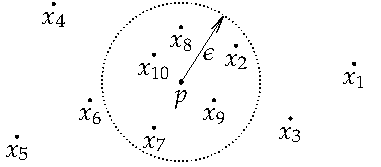
\includegraphics{figures/sequence-convergence-metric}
\caption{Sequence converging to $p$.  The first 10 points 
are shown and $M=7$ for this $\epsilon$.\label{fig:sequence-convergence-metric}}
\end{myfigureht}
\end{defn}

Let us prove that the limit is unique.  The proof is almost
identical (word for word) to the proof of the same fact for sequences of
real numbers,
\propref{prop:limisunique}.
Proofs of many results we know for sequences of real numbers can be
adapted to
the more general settings of metric spaces.  We must replace $\abs{x-y}$
with $d(x,y)$ in the proofs and apply the triangle inequality correctly.

\begin{prop} \label{prop:mslimisunique}
A convergent sequence in a metric space has a unique limit.
\end{prop}

\begin{proof}
%NOTE: should be word for word the same as 2.1.6
Suppose the sequence $\{ x_n \}$ has limits $x$ and $y$.
Take an arbitrary $\epsilon > 0$.
From the definition find an $M_1$ such that for all $n \geq M_1$,
$d(x_n,x) < \nicefrac{\epsilon}{2}$.  Similarly find an $M_2$
such that for all $n \geq M_2$, we have
$d(x_n,y) < \nicefrac{\epsilon}{2}$.  Now take an $n$ such that
$n \geq M_1$ and also $n \geq M_2$, and estimate
\begin{equation*}
\begin{split}
d(y,x)
& \leq
d(y,x_n) + d(x_n,x) \\
& <
\frac{\epsilon}{2} + \frac{\epsilon}{2} = \epsilon .
\end{split}
\end{equation*}
As $d(y,x) < \epsilon$ for all $\epsilon > 0$, then $d(x,y) = 0$
and $y=x$.  Hence the limit (if it exists) is unique.
\end{proof}

The proofs of the following propositions are left as exercises.

\begin{prop} \label{prop:msconvbound}
A convergent sequence in a metric space is bounded.
\end{prop}

\begin{prop} \label{prop:msconvifa}
A sequence $\{ x_n \}$ in a metric space $(X,d)$ converges to $p \in X$
if and only
if there exists a sequence $\{ a_n \}$ of real numbers such that
\begin{equation*}
d(x_n,p) \leq a_n \quad \text{for all } n \in \N,
\end{equation*}
and
\begin{equation*}
\lim_{n\to\infty} a_n = 0.
\end{equation*}
\end{prop}

\begin{prop} \label{prop:mssubseq}
Let $\{ x_n \}$ be a sequence in a metric space $(X,d)$.
\begin{enumerate}[(i)]
\item If $\{ x_n \}$ converges to $p \in X$, then every subsequence $\{ x_{n_k} \}$
converges to $p$.
\item If for some $K \in \N$ the $K$-tail $\{ x_n \}_{n=K+1}^\infty$
converges to $p \in X$, then
 $\{ x_n \}$ converges to $p$.
\end{enumerate}
\end{prop}

\begin{example}
Take $C([0,1],\R)$ be the set of continuous functions with the metric being
the uniform metric.  We saw that we obtain a metric space.
If we look at the definition of convergence, we notice that it is identical
to uniform convergence.  That is, $\{ f_n \}$ converges uniformly if and only
if it converges in the metric space sense.
\end{example}

\begin{remark}
It is perhaps surprising that on the set of functions $f \colon [a,b] \to
\R$ (continuous or not)
there is no metric that gives pointwise convergence.  Although the proof of
this fact is beyond the scope of this book.
\end{remark}

\subsection{Convergence in euclidean space}

In the euclidean space $\R^n$, a sequence converges if and only if every
component converges:

\begin{prop} \label{prop:msconveuc}
Let $\{ x_j \}_{j=1}^\infty$ be a sequence in $\R^n$,
where we write $x_j = \bigl(x_{j,1},x_{j,2},\ldots,x_{j,n}\bigr) \in \R^n$.
Then $\{ x_j \}_{j=1}^\infty$ converges if and only if
$\{ x_{j,k} \}_{j=1}^\infty$ converges for every $k=1,2,\ldots,n$, in which case
\begin{equation*}
\lim_{j\to\infty}
x_j =
\Bigl(
\lim_{j\to\infty} x_{j,1},
\lim_{j\to\infty} x_{j,2},
\ldots,
\lim_{j\to\infty} x_{j,n}
\Bigr) .
\end{equation*}
\end{prop}

\begin{proof}
Suppose
the sequence
$\{ x_j \}_{j=1}^\infty$ converges to
$y = (y_1,y_2,\ldots,y_n) \in \R^n$.
Given $\epsilon > 0$, there exists an $M$, such that for all
$j \geq M$, we have
\begin{equation*}
d(y,x_j) < \epsilon.
\end{equation*}
Fix some $k=1,2,\ldots,n$.  For all $j \geq M$,
\begin{equation*}
\bigl\lvert y_k - x_{j,k} \bigr\rvert
=
\sqrt{{\bigl(y_k - x_{j,k} \bigr)}^2}
\leq
\sqrt{\sum_{\ell=1}^n {\bigl(y_\ell-x_{j,\ell}\bigr)}^2}
= d(y,x_j) < \epsilon .
\end{equation*}
Hence the sequence $\{ x_{j,k} \}_{j=1}^\infty$ converges to $y_k$.

For the other direction, suppose 
$\{ x_{j,k} \}_{j=1}^\infty$ converges to $y_k$ for every $k=1,2,\ldots,n$.
Given $\epsilon > 0$, pick an $M$, such that if $j \geq M$, then 
$\bigl\lvert y_k-x_{j,k} \bigr\rvert < \nicefrac{\epsilon}{\sqrt{n}}$ for all
$k=1,2,\ldots,n$.  Then
\begin{equation*}
d(y,x_j)
=
\sqrt{\sum_{k=1}^n {\bigl(y_k-x_{j,k}\bigr)}^2}
<
\sqrt{\sum_{k=1}^n {\left(\frac{\epsilon}{\sqrt{n}}\right)}^2}
=
\sqrt{\sum_{k=1}^n \frac{{\epsilon^2}}{n}}
= \epsilon .
\end{equation*}
That is, the sequence $\{ x_j \}$ converges to
$y = (y_1,y_2,\ldots,y_n) \in \R^n$.
\end{proof}

\begin{example}
As we said, the set $\C$ of complex numbers $z = x+iy$ is considered 
as the metric space $\R^2$.  The proposition says that the
sequence $\{ z_j \}_{j=1}^\infty = \{ x_j + iy_j \}_{j=1}^\infty$ converges
to $z = x+iy$
if and only if $\{ x_j \}$ converges to $x$ and 
$\{ y_j \}$ converges to $y$.
\end{example}

\subsection{Convergence and topology}

The topology---the set of open sets of a space---encodes which
sequences converge.

\begin{prop} \label{prop:msconvtopo}
Let $(X,d)$ be a metric space and $\{x_n\}$ a sequence in $X$.  Then
$\{ x_n \}$ converges to $x \in X$ if and only if for every open neighborhood
$U$ of $x$, there exists an $M \in \N$ such that for all $n \geq M$,
we have $x_n \in U$.
\end{prop}

\begin{proof}
Suppose $\{ x_n \}$ converges to $x$.  Let $U$ be an open neighborhood
of $x$, then there exists an $\epsilon > 0$ such that $B(x,\epsilon) \subset
U$.  As the sequence converges, find an $M \in \N$ such that for all $n \geq
M$, we have $d(x,x_n) < \epsilon$, or in other words $x_n \in B(x,\epsilon)
\subset U$.

Let us prove the other direction.  Given $\epsilon > 0$, let $U :=
B(x,\epsilon)$ be the neighborhood of $x$.  Then there is an $M \in \N$
such that for $n \geq M$, we have $x_n \in U = B(x,\epsilon)$ or in other
words, $d(x,x_n) < \epsilon$.
\end{proof}

A closed set contains the limits of its convergent sequences.

\begin{prop} \label{prop:msclosedlim}
Let $(X,d)$ be a metric space, $E \subset X$ a closed set,
and $\{ x_n \}$ a sequence in $E$ that converges to some $x \in X$.
Then $x \in E$.
\end{prop}

\begin{proof}
Let us prove the contrapositive.
Suppose $\{ x_n \}$ is a sequence in $X$ that converges to $x \in E^c$.
As $E^c$ is open, \propref{prop:msconvtopo} says that there is
an $M$ such that for all $n \geq M$,
$x_n \in E^c$.  So $\{ x_n \}$  is not a sequence in $E$.
\end{proof}

To take a closure of a set $A$, we take $A$, and we throw in 
points that are limits of sequences in $A$.

\begin{prop} \label{prop:msclosureapprseq}
Let $(X,d)$ be a metric space and $A \subset X$.
Then $x \in \widebar{A}$ if and only if there exists a sequence $\{ x_n \}$ of
elements in $A$ such that $\lim\, x_n = x$.
\end{prop}

\begin{proof}
Let $x \in \widebar{A}$.  For every $n \in \N$,
by
\propref{prop:msclosureappr} there
exists a point $x_n \in B(x,\nicefrac{1}{n}) \cap A$.
As $d(x,x_n) < \nicefrac{1}{n}$, we have $\lim\, x_n = x$.

For the other direction, see \exerciseref{exercise:reverseclosedseq}.
\end{proof}

\subsection{Exercises}

\begin{exercise} \label{exercise:reverseclosedseq}
Finish the proof of 
\propref{prop:msclosureapprseq}.
Let $(X,d)$ be a metric space and
let $A \subset X$.  Let $E$ be the set of all $x \in X$ such that there
exists a sequence $\{ x_n \}$ in $A$ that converges to $x$.  Show 
$E = \widebar{A}$.
\end{exercise}

\begin{exercise}
\leavevmode
\begin{enumerate}[a)]
\item
Show that $d(x,y) := \min \{ 1, \abs{x-y} \}$ defines a metric on $\R$.
\item
Show that a sequence converges in $(\R,d)$ if and only if it converges
in the standard metric.
\item
Find a bounded sequence in $(\R,d)$ that
contains no convergent subsequence.
\end{enumerate}
\end{exercise}

\begin{exercise}
Prove \propref{prop:msconvbound}.
\end{exercise}

\begin{exercise}
Prove \propref{prop:msconvifa}.
\end{exercise}

\begin{exercise}
Suppose $\{x_n\}_{n=1}^\infty$ converges to $x$.  Suppose $f \colon \N
\to \N$ is a one-to-one function.  Show that
$\{ x_{f(n)} \}_{n=1}^\infty$ converges to $x$.
\end{exercise}

\begin{exercise}
Let $(X,d)$ be a metric space where $d$ is the discrete metric.  Suppose 
$\{ x_n \}$ is a convergent sequence in $X$.  Show that there exists
a $K \in \N$ such that for all $n \geq K$, we have $x_n = x_K$.
\end{exercise}

\begin{exercise}
A set $S \subset X$ is said to be \emph{\myindex{dense}} in $X$ if
$X \subset \widebar{S}$ or in other words if for every $x \in X$,
there exists a sequence $\{ x_n \}$ in $S$ that converges to $x$.  Prove
that $\R^n$ contains a countable dense subset.
\end{exercise}

\begin{exercise}[Tricky]
Suppose $\{ U_n \}_{n=1}^\infty$ is a decreasing ($U_{n+1} \subset U_n$ for
all $n$) sequence of open sets in a metric space $(X,d)$ such that
$\bigcap_{n=1}^\infty U_n = \{ p \}$ for some $p \in X$.  Suppose 
$\{ x_n \}$ is a sequence of points in $X$ such that $x_n \in U_n$.  Does
$\{ x_n \}$ necessarily converge to $p$?  Prove or construct a counterexample.
\end{exercise}

\begin{exercise}
Let $E \subset X$ be closed and
let $\{ x_n \}$ be a sequence in $X$ converging to $p \in X$.  Suppose
$x_n \in E$ for infinitely many $n \in \N$.  Show $p \in E$.
\end{exercise}

\begin{exercise} \label{exercise:extendedrealsmetric}
Take $\R^* = \{ -\infty \} \cup \R \cup \{ \infty \}$ be the extended reals.
Define $d(x,y) := \bigl\lvert \frac{x}{1+\abs{x}} - \frac{y}{1+\abs{y}}
\bigr\rvert$
if $x, y \in \R$,
define $d(\infty,x) := \bigl\lvert 1 - \frac{x}{1+\abs{x}} \bigr\rvert$,
$d(-\infty,x) := \bigl\lvert 1 + \frac{x}{1+\abs{x}} \bigr\rvert$
for all $x \in \R$, and
let $d(\infty,-\infty) := 2$.
\begin{enumerate}[a)]
\item
Show that $(\R^*,d)$ is a metric space.
\item
Suppose $\{ x_n \}$ is a sequence of real numbers such that
for every $M \in \R$, there exists an $N$ such that
$x_n \geq M$ for all $n \geq N$.  Show that $\lim\, x_n = \infty$ in
$(\R^*,d)$.
\item
Show that a sequence of real numbers converges to a real number
in $(\R^*,d)$ if and
only if it converges in $\R$ with the standard metric.
\end{enumerate}
\end{exercise}

\begin{exercise}
Suppose $\{ V_n \}_{n=1}^\infty$ is a sequence of open sets
in $(X,d)$
such that $V_{n+1} \supset V_n$ for all $n$.  Let $\{ x_n \}$ be a sequence
such that $x_n \in V_{n+1} \setminus V_n$ and suppose 
$\{ x_n \}$ converges to $p \in X$.  Show that $p \in \partial V$
where $V = \bigcup_{n=1}^\infty V_n$.
\end{exercise}

\begin{exercise}
Prove \propref{prop:mssubseq}.
\end{exercise}

\begin{exercise}
Let $(X,d)$ be a metric space and $\{ x_n \}$ a sequence in $X$.
Prove that $\{ x_n \}$ converges to $p \in X$
if and only if
every subsequence of $\{ x_n \}$ has a subsequence that
converges to $p$.
\end{exercise}

\begin{exercise}
Consider $\R^n$, and let $d$ be the standard euclidean metric.
Let $d'(x,y) := \sum_{\ell=1}^n \abs{x_\ell-y_\ell}$
and $d''(x,y) := \max \{ \abs{x_1-y_1},\abs{x_2-y_2},\cdots,\abs{x_n-y_n}
\}$.
\begin{enumerate}[a)]
\item
Use \exerciseref{exercise:mscross}, to show that
$(\R^n,d')$ and
$(\R^n,d'')$ are metric spaces.
\item
Let $\{ x_j \}_{j=1}^\infty$ be a sequence in $\R^n$ and $p \in \R^n$.
Prove that the following statements are equivalent:
\begin{enumerate}[(1)]
\item
$\{ x_j \}$ converges to $p$ in $(\R^n,d)$.
\item
$\{ x_j \}$ converges to $p$ in $(\R^n,d')$.
\item
$\{ x_j \}$ converges to $p$ in $(\R^n,d'')$.
\end{enumerate}
\end{enumerate}
\end{exercise}

%%%%%%%%%%%%%%%%%%%%%%%%%%%%%%%%%%%%%%%%%%%%%%%%%%%%%%%%%%%%%%%%%%%%%%%%%%%%%%

\sectionnewpage
\section{Completeness and compactness}
\label{sec:metcompact}

\sectionnotes{2 lectures}

\subsection{Cauchy sequences and completeness}

Just like with sequences of real numbers we define Cauchy sequences.

\begin{defn}
Let $(X,d)$ be a metric space.
A sequence $\{ x_n \}$ in $X$ is a \emph{\myindex{Cauchy sequence}} if
for every $\epsilon > 0$ there exists an $M \in \N$ such that
for all $n \geq M$ and all $k \geq M$, we have
\begin{equation*}
d(x_n, x_k) < \epsilon .
\end{equation*}
\end{defn}

The definition is again simply a translation of the concept
from the real numbers to metric spaces.  So a sequence of real
numbers is Cauchy in the sense of \chapterref{seq:chapter} if and only if
it is Cauchy in the sense above, provided we equip the real numbers with
the standard metric $d(x,y) = \abs{x-y}$.

\begin{prop}
A convergent sequence in a metric space is Cauchy.
\end{prop}

\begin{proof}
Suppose $\{ x_n \}$ converges to $x$.
Given $\epsilon > 0$, there is an $M$ such that for all $n \geq M$,
we have $d(x,x_n) < \nicefrac{\epsilon}{2}$.  Hence
for all $n,k \geq M$, we have
$d(x_n,x_k) \leq d(x_n,x) + d(x,x_k) < \nicefrac{\epsilon}{2} +
\nicefrac{\epsilon}{2} = \epsilon$.
\end{proof}

\begin{defn}
Let $(X,d)$ be a metric space.  We say $X$ is
\emph{\myindex{complete}} or \emph{\myindex{Cauchy-complete}}
if every Cauchy sequence $\{ x_n \}$ in $X$
converges to an $x \in X$.
\end{defn}

\begin{prop}
The space $\R^n$ with the standard metric is a complete metric space.
\end{prop}

For $\R = \R^1$ completeness was proved in \chapterref{seq:chapter}.  The proof of
the proposition above is a reduction to the one-dimensional case.

\begin{proof}
Let $\{ x_j \}_{j=1}^\infty$ be a Cauchy sequence
in $\R^n$, where we write $x_j = \bigl(x_{j,1},x_{j,2},\ldots,x_{j,n}\bigr) \in \R^n$.
As the sequence is Cauchy, given $\epsilon > 0$, there exists an $M$ such that for all
$i,j \geq M$,
\begin{equation*}
d(x_i,x_j) < \epsilon.
\end{equation*}

Fix some $k=1,2,\ldots,n$.  For $i,j \geq M$,
\begin{equation*}
\bigl\lvert x_{i,k} - x_{j,k} \bigr\rvert
=
\sqrt{{\bigl(x_{i,k} - x_{j,k}\bigr)}^2}
\leq
\sqrt{\sum_{\ell=1}^n {\bigl(x_{i,\ell}-x_{j,\ell}\bigr)}^2}
= d(x_i,x_j) < \epsilon .
\end{equation*}
Hence the sequence $\{ x_{j,k} \}_{j=1}^\infty$ is Cauchy.  As $\R$ is
complete the sequence converges; there exists a $y_k \in \R$ such that
$y_k = \lim_{j\to\infty} x_{j,k}$.
Write $y = (y_1,y_2,\ldots,y_n) \in \R^n$.
By \propref{prop:msconveuc}, $\{ x_j \}$ converges
to $y \in \R^n$, and hence $\R^n$ is complete.
\end{proof}

A subset of $\R^n$ with the subspace metric need not be
complete.  For example, $(0,1]$ with the subspace metric is not
complete as $\{ \nicefrac{1}{n} \}$ is a Cauchy sequence in $(0,1]$
with no limit in $(0,1]$.  But see also
\exerciseref{exercise:closedcomplete}.

In the language of metric spaces,
the results on continuity of section \sectionref{sec:liminter},
say that the metric space
$C([a,b],\R)$ of \exampleref{example:msC01} is complete.
The proof follows by \myquote{unrolling the definitions,} 
and is left as an exercise.

\begin{prop} \label{prop:CabRcomplete}
The space of continuous functions $C([a,b],\R)$ with the uniform
norm as metric is a complete metric space.
\end{prop}

Once we have one complete metric space, any closed subspace is
also a complete metric space.  After all, one way
to think of a closed set is that it contains all points
that can be reached from the set via a sequence.
The proof is again an exercise.

\begin{prop} \label{prop:closedcomplete}
Suppose $(X,d)$ is a complete metric space and $E \subset X$
is closed, then $E$ is a complete metric space with the subspace topology.
\end{prop}

\subsection{Compactness}

\begin{defn}
Let $(X,d)$ be a metric space and $K \subset X$. 
The set $K$ is said to be \emph{\myindex{compact}}
if for any collection
of open sets $\{ U_{\lambda} \}_{\lambda \in I}$ such that
\begin{equation*}
K \subset \bigcup_{\lambda \in I} U_\lambda ,
\end{equation*}
there exists a finite subset
$\{ \lambda_1, \lambda_2,\ldots,\lambda_k \} \subset I$
such that
\begin{equation*}
K \subset \bigcup_{j=1}^k U_{\lambda_j} .
\end{equation*}
\end{defn}

A collection of open sets $\{ U_{\lambda} \}_{\lambda \in I}$ as above is
said to be an \emph{\myindex{open cover}} of $K$.  So a way to say that
$K$ is compact is to say that \emph{every open cover of $K$ has a finite
\myindex{subcover}}.

\begin{example}
Let $\R$ be the metric space with the standard metric.

The set $\R$ is not compact.  Proof: Take the sets $U_j := (-j,j)$.
Any $x \in \R$ is in some $U_j$ (by the
\hyperref[thm:arch:i]{Archimedean property}), so we have an open cover.
Suppose we have a finite
subcover $\R \subset U_{j_1} \cup U_{j_2} \cup \cdots \cup U_{j_k}$,
and suppose $j_1 < j_2 < \cdots < j_k$.  Then $\R \subset U_{j_k}$, but that is
a contradiction as $j_k \in \R$ on one hand and $j_k \notin U_{j_k} =
(-j_k,j_k)$ on the
other.

The set $(0,1) \subset \R$ is also not compact.  Proof:  Take the 
sets $U_{j} := (\nicefrac{1}{j},1-\nicefrac{1}{j})$ for $j=3,4,5,\ldots$.
As above $(0,1) = \bigcup_{j=3}^\infty U_j$.  And similarly as above,
if there exists a finite subcover, then there is one $U_j$ such that $(0,1)
\subset U_j$, which again leads to a contradiction.

The set $\{ 0 \} \subset \R$ is compact.  Proof: Given any open cover $\{
U_{\lambda} \}_{\lambda \in I}$, there must exist a $\lambda_0$ such that $0
\in U_{\lambda_0}$ as it is a cover.  But then $U_{\lambda_0}$ gives a
finite subcover.

We will prove below that $[0,1]$, and in fact any closed and bounded
interval $[a,b]$ is compact.
\end{example}

\begin{prop}
Let $(X,d)$ be a metric space.  A compact set $K \subset X$ is closed and
bounded.
\end{prop}

\begin{proof}
First, we prove that a compact set is bounded.
Fix $p \in X$.  We have the open cover
\begin{equation*}
K \subset \bigcup_{n=1}^\infty B(p,n) = X .
\end{equation*}
If $K$ is compact, then there exists some set of indices
$n_1 < n_2 < \ldots < n_k$ such that
\begin{equation*}
K \subset \bigcup_{j=1}^k B(p,n_j) = B(p,n_k) .
\end{equation*}
As $K$ is contained in a ball, $K$ is bounded.
See the left-hand side of \figureref{fig:compactbndclosed}.

Next, we show a set that is not closed is not compact.  Suppose 
$\widebar{K} \not= K$, that is, there is a point $x \in \widebar{K}
\setminus K$.
If $y \not= x$, then
$y \notin C(x,\nicefrac{1}{n})$
for $n \in \N$
such that $\nicefrac{1}{n} < d(x,y)$.
Furthermore $x \notin K$, so
\begin{equation*}
K \subset \bigcup_{n=1}^\infty {C(x,\nicefrac{1}{n})}^c .
\end{equation*}
A closed ball is closed, so its complement ${C(x,\nicefrac{1}{n})}^c$ is open, and
we have an open cover.
If we take any
finite collection of indices $n_1 < n_2 < \ldots < n_k$, then 
\begin{equation*}
\bigcup_{j=1}^k {C(x,\nicefrac{1}{n_j})}^c 
=
{C(x,\nicefrac{1}{n_k})}^c 
\end{equation*}
As $x$ is in the closure of $K$,
then
$C(x,\nicefrac{1}{n_k}) \cap K \not= \emptyset$.  So there is no
finite subcover and $K$ is not compact.
See the right-hand side of \figureref{fig:compactbndclosed}.
\end{proof}

\begin{myfigureht}
\subimport*{figures/}{compact_bnd_closed.pdf_t}
\caption{Proving compact set is bounded (left) and closed (right).\label{fig:compactbndclosed}}
\end{myfigureht}

We prove below that 
in a finite-dimensional euclidean space
every closed bounded set is compact.
So closed bounded sets
of $\R^n$ are examples of compact sets.
It is not true that in every metric space, closed and bounded is equivalent
to compact.  A simple example is an incomplete metric space such as
$(0,1)$ with the subspace metric from $\R$.
There are many complete and very useful metric spaces
where closed and bounded is not
enough to give compactness: $C([a,b],\R)$ is a complete metric
space, but the closed unit ball $C(0,1)$ is not compact, see
\exerciseref{exercise:msclbounnotcompt}.  However, see also
\exerciseref{exercise:mstotbound}.

A useful property of compact sets in a metric space is that every
sequence in the set has a convergent subsequence converging
to a point in the set.
Such sets are called
\emph{\myindex{sequentially compact}}.
Let us prove that in the
context of metric spaces, a set is compact if and only if it is sequentially
compact.
First we prove a lemma.

\begin{lemma}[Lebesgue covering lemma%
\footnote{Named after the French mathematician
\href{https://en.wikipedia.org/wiki/Henri_Lebesgue}{Henri L\'eon Lebesgue}
(1875--1941).
The number $\delta$ is sometimes called the \myindex{Lebesgue number} of the
cover.}]\label{ms:lebesgue}
\index{Lebesgue covering lemma}
Let $(X,d)$ be a metric space and $K \subset X$.  Suppose 
every sequence in $K$ has a subsequence convergent in $K$.  Given
an open cover $\{ U_\lambda \}_{\lambda \in I}$ of $K$, there exists a
$\delta > 0$ such that for every $x \in K$, there exists a $\lambda \in I$
with $B(x,\delta) \subset U_\lambda$.
\end{lemma}

\begin{proof}
We prove the lemma by contrapositive.
If the conclusion is not true, then
there is
an open cover $\{ U_\lambda \}_{\lambda \in I}$ of $K$ with
the following property.
For every $n \in \N$ there exists an $x_n \in K$ such that
$B(x_n,\nicefrac{1}{n})$ is not a subset of any $U_\lambda$.
Take any $x \in K$.  There is
a $\lambda \in I$ such that $x \in U_\lambda$.  As $U_\lambda$ is open,
there is an $\epsilon > 0$ 
such that $B(x,\epsilon) \subset U_\lambda$.  Take $M$ such that
$\nicefrac{1}{M} < \nicefrac{\epsilon}{2}$.  If $y \in 
B(x,\nicefrac{\epsilon}{2})$ and $n \geq M$, then 
\begin{equation*}
B(y,\nicefrac{1}{n}) \subset
B(y,\nicefrac{1}{M}) \subset
B(y,\nicefrac{\epsilon}{2}) \subset B(x,\epsilon)
\subset U_\lambda ,
\end{equation*}
where 
$B(y,\nicefrac{\epsilon}{2}) \subset B(x,\epsilon)$
follows by triangle inequality.
See \figureref{fig:lebesguedelta}.
In other words, for all $n \geq M$, $x_n \notin B(x,\nicefrac{\epsilon}{2})$. 
The sequence cannot have a subsequence converging to $x$.  As $x \in K$ was
arbitrary we are done.
\end{proof}

\begin{myfigureht}
\subimport*{figures/}{lebesguedelta.pdf_t}
\caption{Proof of Lebesgue covering lemma.
Note that $B(y,\nicefrac{\epsilon}{2}) \subset
B(x,\epsilon)$ by triangle inequality.\label{fig:lebesguedelta}}
\end{myfigureht}

It is important to recognize what the lemma says.  It says that
if $K$ is sequentially compact, then given any
cover there is a single $\delta > 0$.  The $\delta$ depends on the cover,
but of course it does not depend on $x$.

For example, let $K := [-10,10]$ and for $n \in \Z$ let $U_n :=
(n,n+2)$ define sets in an open cover.
Take $x \in K$. There is an $n \in \Z$, 
such that $n \leq x < n+1$.
If $n \leq x < n+\nicefrac{1}{2}$, then
$B\bigl(x,\nicefrac{1}{2}\bigr) \subset U_{n-1}$.
If $n+ \nicefrac{1}{2} \leq x < n+1$, then
$B\bigl(x,\nicefrac{1}{2}\bigr) \subset U_{n}$.  So $\delta =
\nicefrac{1}{2}$.  If instead we let $U'_n :=
\bigl(\frac{n}{2},\frac{n+2}{2} \bigr)$, then we again obtain an open
cover, but now the best $\delta$ we can find is $\nicefrac{1}{4}$.

On the other hand, $\N \subset \R$ is not sequentially compact.
It is an exercise to find a cover for which no $\delta > 0$ works.


\begin{thm} \label{thm:mscompactisseqcpt}
Let $(X,d)$ be a metric space.  Then $K \subset X$ is compact if
and only if every sequence in $K$ has a subsequence converging to
a point in $K$.
\end{thm}

\begin{proof}
Claim: \emph{Let $K \subset X$ be a subset of $X$ and
$\{ x_n \}$ a sequence in $K$.  Suppose that for each $x \in K$,
there is a ball $B(x,\alpha_x)$ for some $\alpha_x > 0$ such that
$x_n \in B(x,\alpha_x)$ for only finitely many $n \in \N$.
Then $K$ is not compact.}

Proof of the claim:
Notice
\begin{equation*}
K \subset \bigcup_{x \in K} B(x,\alpha_x) .
\end{equation*}
Any finite collection of these balls is going to contain only finitely many
$x_n$.  Thus for any finite collection of such balls there is an $x_n \in K$
that is not in the union.  Therefore, $K$ is not compact and the claim is
proved.

So suppose that $K$ is compact and $\{ x_n \}$ is a sequence in $K$.
Then there exists an $x \in K$ such that
for any $\delta > 0$,
$B(x,\delta)$ contains $x_k$ for infinitely many $k \in \N$.
We define the subsequence inductively.
The ball $B(x,1)$ contains some $x_k$ so let $n_1 := k$.
Suppose $n_{j-1}$ is defined.
There must exist a $k > n_{j-1}$
such that $x_k \in B(x,\nicefrac{1}{j})$.  So define
$n_j := k$.
We now posses a subsequence $\{ x_{n_j} \}_{j=1}^\infty$.
Since
$d(x,x_{n_j}) < \nicefrac{1}{j}$,  \propref{prop:msconvifa} says
$\lim\, x_{n_j} = x$.

For the other direction, suppose every sequence in $K$
has a 
subsequence converging in $K$.
Take
an open cover $\{ U_\lambda \}_{\lambda \in I}$ of $K$.
Using the Lebesgue covering lemma above, find a $\delta > 0$
such that for every $x \in K$, there is a $\lambda \in I$ with
$B(x,\delta) \subset U_\lambda$.

Pick $x_1 \in K$ and find $\lambda_1 \in I$ such that $B(x_1,\delta) \subset
U_{\lambda_1}$.
If $K \subset U_{\lambda_1}$, we stop as we have found a
finite subcover.
Otherwise, there must be
a point $x_2 \in K \setminus U_{\lambda_1}$.
Note that $d(x_2,x_1) \geq \delta$.
There must exist some $\lambda_2 \in I$ such that
$B(x_2,\delta) \subset U_{\lambda_2}$.
We work inductively.  Suppose $\lambda_{n-1}$ is defined.
Either
$U_{\lambda_1} \cup
U_{\lambda_2} \cup \cdots \cup
U_{\lambda_{n-1}}$ is a finite cover of $K$, in which case we
stop, or
there must be 
a point $x_n \in K \setminus \bigl( U_{\lambda_1} \cup
U_{\lambda_2} \cup \cdots \cup
U_{\lambda_{n-1}}\bigr)$.
Note that $d(x_n,x_j) \geq \delta$ for all $j = 1,2,\ldots,n-1$.
Next, there must be some $\lambda_n \in I$
such that $B(x_n,\delta) \subset U_{\lambda_n}$.
See \figureref{fig:seqcompactiscompact}.

\begin{myfigureht}
\subimport*{figures/}{seqcompactiscompact.pdf_t}
\caption{Covering $K$ by $U_{\lambda}$.  The points
$x_1,x_2,x_3,x_4$, 
the three sets 
$U_{\lambda_1}$,
$U_{\lambda_2}$,
$U_{\lambda_2}$,
and 
the first three balls
of radius $\delta$ are drawn.\label{fig:seqcompactiscompact}}
\end{myfigureht}

Either at some point we obtain a finite subcover of $K$,
or we obtain an
infinite
sequence $\{ x_n \}$ as above.
For contradiction, suppose that
there is no finite subcover and we have the sequence $\{ x_n \}$.
For all $n$ and $k$, $n \not= k$, 
we have $d(x_n,x_k) \geq \delta$,
so no subsequence of $\{ x_n \}$ can be
Cauchy.  Hence no subsequence of $\{ x_n \}$ can be convergent,
which is a contradiction.
\end{proof}

\begin{example}
The Bolzano--Weierstrass theorem for sequences of real numbers
(\thmref{thm:bwseq})
says that any bounded sequence in $\R$ has a convergent
subsequence.  Therefore, any sequence in a closed interval $[a,b] \subset \R$ has 
a convergent subsequence.  The limit must also be in $[a,b]$ as limits
preserve non-strict inequalities.  Hence a closed bounded interval $[a,b]
\subset \R$ is compact.
\end{example}

\begin{prop}
Let $(X,d)$ be a metric space and let $K \subset X$ be compact.  If
$E \subset K$ is a closed set, then $E$ is compact.
\end{prop}

Because $K$ is closed, then $E$ is closed in $K$ if
and only if it is closed in $X$,
see \propref{prop:topology:subspacesame}.

\begin{proof}
Let $\{ x_n \}$ be a sequence in $E$.  It is also a sequence in $K$.
Therefore, it has a convergent subsequence $\{ x_{n_j} \}$ that converges to
some $x \in K$.  As $E$ is closed the limit of a sequence in $E$ is also in $E$
and so $x \in E$.  Thus $E$ must be compact.
\end{proof}

\begin{thm}[Heine--Borel%
\footnote{Named after the German mathematician 
\href{https://en.wikipedia.org/wiki/Eduard_Heine}{Heinrich Eduard Heine}
(1821--1881),
and the French mathematician
\href{https://en.wikipedia.org/wiki/\%C3\%89mile_Borel}{F\'elix \'Edouard Justin \'Emile Borel}
(1871--1956).}]%
\index{Heine--Borel theorem}
\label{thm:msbw}
A closed bounded subset $K \subset \R^n$ is compact.
\end{thm}

So subsets of $\R^n$ are compact if and only if they are closed and bounded,
a condition that is much easier to check.
Let us reiterate that the Heine--Borel theorem only holds for $\R^n$ and not
for metric spaces in general.  In general, compact implies closed and
bounded, but not vice versa.

\begin{proof}
For $\R = \R^1$ if $K \subset \R$ is closed and bounded, then
any sequence $\{ x_k \}$ in $K$ is bounded, so it has a convergent
subsequence by
Bolzano--Weierstrass theorem (\thmref{thm:bwseq}).
As $K$ is closed, the limit of the subsequence must be an element of
$K$.  So $K$ is compact.

Let us carry out the proof for $n=2$ and leave arbitrary $n$ as an exercise.
As $K \subset \R^2$ is bounded, there exists a set
$B=[a,b]\times[c,d] \subset \R^2$ such that $K \subset B$.  We will show
that $B$ is compact.  Then $K$, being a closed subset of a compact $B$, is
also compact.  

Let $\bigl\{ (x_k,y_k) \bigr\}_{k=1}^\infty$ be a sequence in $B$.  That is,
$a \leq x_k \leq b$ and
$c \leq y_k \leq d$ for all $k$.  A bounded sequence of real numbers
has a convergent
subsequence so there is a subsequence $\{ x_{k_j} \}_{j=1}^\infty$
that is convergent.  The subsequence 
$\{ y_{k_j} \}_{j=1}^\infty$ is also a bounded sequence so there exists
a subsequence
$\{ y_{k_{j_i}} \}_{i=1}^\infty$ that is convergent.  A subsequence of a
convergent sequence is still convergent, so 
$\{ x_{k_{j_i}} \}_{i=1}^\infty$ is convergent.
Let
\begin{equation*}
x := \lim_{i\to\infty} x_{k_{j_i}}
\qquad \text{and} \qquad
y := \lim_{i\to\infty} y_{k_{j_i}} .
\end{equation*}
By \propref{prop:msconveuc},
$\bigl\{ (x_{k_{j_i}},y_{k_{j_i}}) \bigr\}_{i=1}^\infty$ converges to $(x,y)$.
Furthermore, as $a \leq x_k \leq b$ and
$c \leq y_k \leq d$ for all $k$, we know that $(x,y) \in B$.
\end{proof}

\begin{example}
The discrete metric provides interesting counterexamples again.
Let $(X,d)$ be a metric space with the discrete metric, that is $d(x,y) = 1$
if $x \not= y$.  Suppose
$X$ is an infinite set.  Then
\begin{enumerate}[(i)]
\item $(X,d)$ is a complete metric space.
\item Any subset $K \subset X$ is closed and bounded.
\item A subset $K \subset X$ is compact if and only if it is a finite set.
\item The conclusion of the Lebesgue covering lemma is always satisfied with
e.g. $\delta = \nicefrac{1}{2}$, even for noncompact $K \subset X$.
\end{enumerate}
The proofs
of the statements above are either trivial or are relegated to the exercises
below.
\end{example}

\begin{remark}
A subtle issue with Cauchy sequences, completeness, compactness,
and convergence is that compactness and convergence only depend on the
topology, that is, on which sets are the open sets.  On the other hand,
Cauchy sequences and completeness depend on the actual metric.
See \exerciseref{exercise:cauchydepndsonmetric}.
\end{remark}

\subsection{Exercises}

\begin{exercise}
Let $(X,d)$ be a metric space and $A$ a finite subset of $X$.
Show that $A$ is compact.
\end{exercise}

\begin{samepage}
\begin{exercise}
Let $A = \{ \nicefrac{1}{n} : n \in \N \} \subset \R$.
\begin{enumerate}[a)]
\item
Show that $A$ is
not compact directly using the definition.
\item
Show that $A \cup \{ 0 \}$ is
compact directly using the definition.
\end{enumerate}
\end{exercise}
\end{samepage}


\begin{exercise}
Let $(X,d)$ be a metric space with the discrete metric.
\begin{enumerate}[a)]
\item
Prove that $X$ is complete.
\item
Prove that $X$ is compact if and only if $X$ is a finite set.
\end{enumerate}
\end{exercise}

\begin{exercise}
\leavevmode
\begin{enumerate}[a)]
\item
Show that the union of finitely many compact sets is a compact set.
\item
Find an example where the union of infinitely many compact sets is not
compact.
\end{enumerate}
\end{exercise}

\begin{exercise}
Prove \thmref{thm:msbw} for arbitrary dimension.
Hint: The trick is to use the correct notation.
\end{exercise}

\begin{exercise}
Show that a compact set $K$ is a complete metric space (using the subspace
metric).
\end{exercise}

\begin{exercise} \label{exercise:CabRcomplete}
Let $C([a,b],\R)$ be the metric space as in \exampleref{example:msC01}.  Show that
$C([a,b],\R)$ is a complete metric space.
\end{exercise}

\begin{exercise}[Challenging] \label{exercise:msclbounnotcompt}
Let $C([0,1],\R)$ be the metric space of \exampleref{example:msC01}.  Let $0$
denote the zero function.  Then show that the closed ball
$C(0,1)$ is not compact (even though it is closed and bounded).
Hints: Construct a sequence of distinct continuous functions $\{ f_n \}$ such that
$d(f_n,0) = 1$ and $d(f_n,f_k) = 1$ for all $n \not= k$.  Show that
the set $\{ f_n : n \in \N \} \subset C(0,1)$ is closed but not compact.
See \chapterref{fs:chapter} for inspiration.
\end{exercise}

\begin{exercise}[Challenging]
Show that there exists a metric on $\R$ that makes $\R$ into a compact set.
\end{exercise}

\begin{exercise}
Suppose $(X,d)$ is complete and suppose we have a countably infinite
collection of nonempty compact sets $E_1 \supset E_2 \supset E_3 \supset
\cdots$.  Prove $\bigcap_{j=1}^\infty E_j \not= \emptyset$.
\end{exercise}

\begin{exercise}[Challenging]
Let $C([0,1],\R)$ be the metric space of \exampleref{example:msC01}.
Let $K$ be the set of $f \in C([0,1],\R)$ such that
$f$ is equal to a quadratic polynomial, i.e.\ $f(x) = a+bx+cx^2$, and such that
$\abs{f(x)} \leq 1$ for all $x \in [0,1]$,
that is $f \in C(0,1)$.  Show that $K$ is compact.
\end{exercise}

\begin{exercise}[Challenging] \label{exercise:mstotbound}
Let $(X,d)$ be a complete metric space.
Show that $K \subset X$ is compact if and only if $K$ is closed
and such that for every $\epsilon > 0$
there exists a finite set of points $x_1,x_2,\ldots,x_n$ with
$K \subset \bigcup_{j=1}^n B(x_j,\epsilon)$.
Note: Such a set $K$ is said to be \emph{\myindex{totally bounded}},
so in a complete metric space a set is compact if and only
if it is closed and totally bounded.
\end{exercise}

\begin{exercise}
Take $\N \subset \R$ using the standard metric.  Find an open cover of $\N$
such that the conclusion of the Lebesgue covering lemma does not hold.
\end{exercise}

\begin{exercise}
Prove the general \myindex{Bolzano--Weierstrass theorem}:
Any bounded sequence $\{ x_k
\}$ in $\R^n$ has a convergent subsequence.
\end{exercise}

\begin{exercise}
Let $X$ be a metric space and
$C \subset \sP(X)$ the set of nonempty compact subsets of $X$.
Using the Hausdorff metric from \exerciseref{exercise:mshausdorffpseudo},
show that $(C,d_H)$ is a metric space.  That is, show that
if $L$ and $K$ are nonempty compact subsets, then $d_H(L,K) = 0$
if and only if $L=K$.
\end{exercise}

\begin{exercise} \label{exercise:closedcomplete}
Prove \propref{prop:closedcomplete}.  That is,
let $(X,d)$ be a complete metric space and $E \subset X$ a closed set.
Show that $E$ with the subspace metric is a complete metric space.
\end{exercise}

\begin{exercise}
Let $(X,d)$ be an incomplete metric space.  Show that there exists a
closed and bounded set $E \subset X$ that is not compact.
\end{exercise}

\begin{exercise}
Let $(X,d)$ be a metric space and $K \subset X$.
Prove that $K$ is compact as a subset of $(X,d)$ if and only if $K$ is
compact as a subset of itself with the subspace metric.
\end{exercise}

\begin{exercise} \label{exercise:cauchydepndsonmetric}
Consider two metrics on $\R$.
Let $d(x,y) := \abs{x-y}$ be the standard metric,
and let
$d'(x,y) := \bigl\lvert \frac{x}{1+\abs{x}} - \frac{y}{1+\abs{y}}
\bigr\rvert$.
\begin{enumerate}[a)]
\item
Show that $(\R,d')$ is a metric space (if you have done
\exerciseref{exercise:extendedrealsmetric}, the computation is the same).
\item
Show that the topology is the same, that is, a set is open in
$(\R,d)$ if and only if it is open in $(\R,d')$.
\item
Show that a set is compact in
$(\R,d)$ if and only if it is compact in $(\R,d')$.
\item
Show that a sequence converges in $(\R,d)$ if and only if
it converges in $(\R,d')$.
\item
Find a sequence of real numbers that is Cauchy
in $(\R,d')$ but not Cauchy in $(\R,d)$.
\item
While $(\R,d)$ is complete, show that $(\R,d')$ is not complete.
\end{enumerate}
\end{exercise}

\begin{exercise} \label{exercise:relativelycompactseq}
Let $(X,d)$ be a complete metric space.
We say a set $S \subset X$ is \emph{\myindex{relatively compact}}
if the closure $\widebar{S}$ is compact.
Prove that $S \subset X$ is relatively compact if and only if
given any sequence $\{ x_n \}$ in $S$, there exists a subsequence
$\{ x_{n_k} \}$ that converges (in $X$).
\end{exercise}

%%%%%%%%%%%%%%%%%%%%%%%%%%%%%%%%%%%%%%%%%%%%%%%%%%%%%%%%%%%%%%%%%%%%%%%%%%%%%%

\sectionnewpage
\section{Continuous functions}
\label{sec:metcont}

\sectionnotes{1.5--2 lectures}

\subsection{Continuity}

\begin{defn}
Let $(X,d_X)$ and $(Y,d_Y)$ be metric spaces and $c \in X$.
Then $f \colon X \to Y$ is
\emph{continuous at $c$}\index{continuous at $c$}
if for every $\epsilon > 0$
there is a $\delta > 0$ such that whenever $x \in X$ and $d_X(x,c) <
\delta$, then
$d_Y\bigl(f(x),f(c)\bigr) < \epsilon$.

\medskip

When $f \colon X \to Y$ is continuous at all $c \in X$, then we simply say
that $f$ is a \emph{continuous function}\index{continuous function!in a
metric space}\index{function!continuous}.
\end{defn}

The definition agrees with the definition from \chapterref{lim:chapter} when
$f$ is a real-valued function on the real line, if we take the standard
metric on $\R$.

\begin{prop} \label{prop:contiscont}
Let $(X,d_X)$ and $(Y,d_Y)$ be metric spaces.
Then $f \colon X \to Y$ is
continuous at $c \in X$
if and only if for every sequence $\{ x_n \}$ in $X$
converging to $c$, the sequence $\{ f(x_n) \}$ converges
to $f(c)$.
\end{prop}

\begin{proof}
Suppose $f$ is continuous at $c$.  Let $\{ x_n \}$ be a
sequence in $X$ converging to $c$.  Given $\epsilon > 0$,
there is a $\delta > 0$ such that $d_X(x,c) < \delta$ implies
$d_Y\bigl(f(x),f(c)\bigr) < \epsilon$.  So take $M$ such that
for all $n \geq M$, we have $d_X(x_n,c) < \delta$, then
$d_Y\bigl(f(x_n),f(c)\bigr) < \epsilon$.  Hence $\{ f(x_n) \}$
converges to $f(c)$.

On the other hand suppose $f$ is not continuous at $c$.
Then there exists an $\epsilon > 0$,
such that for every $n \in \N$ there exists an $x_n \in X$,
with
$d_X(x_n,c) < \nicefrac{1}{n}$ such that $d_Y\bigl(f(x_n),f(c)\bigr) \geq
\epsilon$.  Then $\{ x_n \}$ converges to $c$, but $\{ f(x_n) \}$
does not converge to $f(c)$.
\end{proof}

\begin{example}
Suppose $f \colon \R^2 \to \R$ is a polynomial.  That is,
\begin{equation*}
f(x,y) =
\sum_{j=0}^d
\sum_{k=0}^{d-j}
a_{jk}\,x^jy^k =
a_{0\,0} + a_{1\,0} \, x +
a_{0\,1} \, y+  
a_{2\,0} \, x^2+  
a_{1\,1} \, xy+  
a_{0\,2} \, y^2+ \cdots +
a_{0\,d} \, y^d ,
\end{equation*}
for some $d \in \N$ (the degree) and $a_{jk} \in \R$.  Then we claim 
$f$ is continuous.  Let $\{ (x_n,y_n) \}_{n=1}^\infty$ be a sequence
in $\R^2$ that converges to $(x,y) \in \R^2$.  We proved that this
means $\lim\, x_n = x$ and $\lim\, y_n = y$.
By \propref{prop:contalg}, we have
\begin{equation*}
\lim_{n\to\infty}
f(x_n,y_n) =
\lim_{n\to\infty}
\sum_{j=0}^d
\sum_{k=0}^{d-j}
a_{jk} \, x_n^jy_n^k 
=
\sum_{j=0}^d
\sum_{k=0}^{d-j}
a_{jk} \, x^jy^k
=
f(x,y) .
\end{equation*}
So $f$ is continuous at $(x,y)$, and as $(x,y)$ was arbitrary $f$ is
continuous everywhere.  Similarly, a
polynomial in $n$ variables is continuous.
\end{example}

Be careful about taking limits separately.  In \exerciseref{exercise:dicontR2}
you are asked to prove that the function defined by $f(x,y) := \frac{xy}{x^2+y^2}$
outside the origin and $f(0,0) := 0$, is not continuous at the origin.  See
\figureref{fig:xyxsqysq}.
However, for any $y$, the function $g(x) := f(x,y)$ is
continuous,
and for any $x$, the function $h(y) := f(x,y)$ is continuous.
\begin{myfigureht}
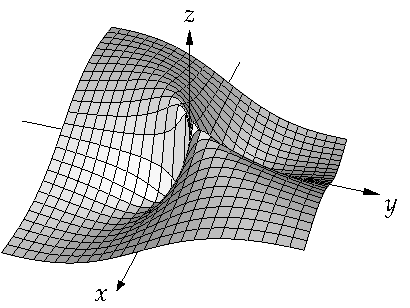
\includegraphics{figures/xyxsqysq}
\caption{Graph of $\frac{xy}{x^2+y^2}$.\label{fig:xyxsqysq}}
\end{myfigureht}

\begin{example}
Let $X$ be a metric space and $f \colon X \to \C$ a complex-valued
function.  We write $f(p) = g(p) + i h(p)$, where $g \colon X \to \R$
and $h \colon X \to \R$ are the real and imaginary parts of $f$.
Then $f$ is continuous at $c \in X$ if and only if its real
and imaginary parts are continuous at $c$.  
This fact follows because $\{ f(p_n) = g(p_n) + i h(p_n) \}_{n=1}^\infty$
converges to $f(p) = g(p) + i h(p)$ if and only if
$\{ g(p_n) \}$ converges to $g(p)$ and
$\{ h(p_n) \}$ converges to $h(p)$.
\end{example}

\subsection{Compactness and continuity}

Continuous maps do not map closed sets to closed sets.  For example,
$f \colon (0,1) \to \R$ defined by $f(x) := x$ takes the set $(0,1)$, which
is closed in $(0,1)$, to the set $(0,1)$, which is not closed in $\R$.
On the other hand continuous maps do preserve compact sets.

\begin{lemma} \label{lemma:continuouscompact}
Let $(X,d_X)$ and $(Y,d_Y)$ be metric spaces
and $f \colon X \to Y$ a continuous function.  If
$K \subset X$ is a compact set, then $f(K)$ is a compact set.
\end{lemma}

\begin{proof}
A sequence in $f(K)$ can be written as
$\{ f(x_n) \}_{n=1}^\infty$, where
$\{ x_n \}_{n=1}^\infty$ is a sequence in $K$.  The set $K$ is compact and
therefore there is a subsequence
$\{ x_{n_j} \}_{j=1}^\infty$ that converges to some $x \in K$.
By continuity,
\begin{equation*}
\lim_{j\to\infty} f(x_{n_j}) = f(x) \in f(K) .
\end{equation*}
So every sequence in $f(K)$ has a subsequence convergent to 
a point in $f(K)$, and $f(K)$ is compact by \thmref{thm:mscompactisseqcpt}.
\end{proof}

As before, $f \colon X \to \R$ achieves an
\emph{\myindex{absolute minimum}} at $c \in X$ if
\begin{equation*}
f(x) \geq f(c) \qquad \text{for all } x \in X.
\end{equation*}
On the other hand, $f$ achieves an 
\emph{\myindex{absolute maximum}} at $c \in X$ if
\begin{equation*}
f(x) \leq f(c) \qquad \text{for all } x \in X.
\end{equation*}

\begin{thm}
Let $(X,d)$ be a compact metric space
and $f \colon X \to \R$ a continuous function.  Then
$f$ is bounded and in fact
$f$ achieves an absolute minimum and an absolute maximum on $X$.
\end{thm}

\begin{proof}
As $X$ is compact and $f$ is continuous, then
$f(X) \subset \R$ is compact.  Hence $f(X)$ is closed
and bounded.  In particular,
$\sup f(X) \in f(X)$ and
$\inf f(X) \in f(X)$, because both the sup and the inf
can be achieved by sequences in $f(X)$ and $f(X)$ is closed.
Therefore, there is some $x \in X$ such that $f(x) = \sup f(X)$
and some $y \in X$ such that $f(y) = \inf f(X)$.
\end{proof}

\subsection{Continuity and topology}

Let us see how to define continuity in terms of the topology, that is,
the open sets.  We have already seen that topology determines which 
sequences converge, and so it is no wonder that the topology also
determines continuity of functions.

\begin{lemma} \label{lemma:mstopocontloc}
Let $(X,d_X)$ and $(Y,d_Y)$ be metric spaces.
A function $f \colon X \to Y$ is continuous at $c \in X$
if and only if for every open neighborhood $U$ of $f(c)$ in $Y$, the set
$f^{-1}(U)$ contains an open neighborhood of $c$ in $X$.
See \figureref{fig:mscontfuncpt}.
\end{lemma}

\begin{myfigureht}
\subimport*{figures/}{mscontfuncpt.pdf_t}
\caption{For every neighborhood $U$ of $f(c)$, the set $f^{-1}(U)$ contains an open
neighborhood $W$ of $c$.\label{fig:mscontfuncpt}}
\end{myfigureht}

\begin{proof}
First suppose that $f$ is continuous at $c$.
Let $U$ be an open neighborhood of $f(c)$
in $Y$, then $B_Y\bigl(f(c),\epsilon\bigr) \subset U$ for some $\epsilon >
0$.  By continuity of $f$, there exists a $\delta > 0$
such that whenever $x$ is such that $d_X(x,c) < \delta$, then
$d_Y\bigl(f(x),f(c)\bigr) < \epsilon$.  In other words,
\begin{equation*}
B_X(c,\delta) \subset f^{-1}\bigl(B_Y\bigl(f(c),\epsilon\bigr)\bigr) \subset
f^{-1}(U) ,
\end{equation*}
and $B_X(c,\delta)$ is an open neighborhood of $c$.

For the other direction,
let $\epsilon > 0$ be given.  If
$f^{-1}\bigl(B_Y\bigl(f(c),\epsilon\bigr)\bigr)$ contains an open
neighborhood $W$ of $c$, it contains a ball.  That is, there is some $\delta > 0$
such that
\begin{equation*}
B_X(c,\delta) \subset W \subset f^{-1}\bigl(B_Y\bigl(f(c),\epsilon\bigr)\bigr) .
\end{equation*}
That means precisely that if $d_X(x,c) < \delta$, then $d_Y\bigl(f(x),f(c)\bigr)
< \epsilon$, and so $f$ is continuous at $c$.
\end{proof}

\begin{thm} \label{thm:mstopocont}
Let $(X,d_X)$ and $(Y,d_Y)$ be metric spaces.  A function $f \colon X \to Y$
is continuous if and only if
for every open $U \subset Y$, $f^{-1}(U)$ is open in $X$.
\end{thm}

The proof follows from \lemmaref{lemma:mstopocontloc} and is left as
an exercise.

\begin{example}
Let $f \colon X \to Y$ be a continuous function.
\thmref{thm:mstopocont} tells us that if $E \subset Y$ is closed, then 
$f^{-1}(E) = X \setminus f^{-1}(E^c)$ is also closed.  Therefore, if
we have a continuous
function $f \colon X \to \R$, then the
\emph{\myindex{zero set}} of $f$, that is, 
$f^{-1}(0) = \{ x \in X :
f(x) = 0 \}$, is closed.  We have just proved the most basic result in
\emph{\myindex{algebraic geometry}}, the study of
zero sets of polynomials:  The zero set of a polynomial is closed.

Similarly the set where $f$ is nonnegative, that is,
$f^{-1}\bigl( [0,\infty) \bigr) = \{ x \in X :
f(x) \geq 0 \}$ is closed.  On the other hand the
set where $f$ is positive,
$f^{-1}\bigl( (0,\infty) \bigr) = \{ x \in X :
f(x) > 0 \}$ is open.  
\end{example}

\subsection{Uniform continuity}

As for continuous
functions on the real line, in the definition of continuity
it is sometimes convenient to be able to pick
one $\delta$ for all points.

\begin{defn}
Let $(X,d_X)$ and $(Y,d_Y)$ be metric spaces.
Then $f \colon X \to Y$ is
\emph{uniformly continuous}\index{uniformly continuous!in a metric space}
if for every $\epsilon > 0$
there is a $\delta > 0$ such that whenever $p,q \in X$ and $d_X(p,q) <
\delta$, then
$d_Y\bigl(f(p),f(q)\bigr) < \epsilon$.
\end{defn}

A uniformly continuous function is continuous, but not necessarily
vice versa as we have seen.

\begin{thm} \label{thm:Xcompactfunifcont}
Let $(X,d_X)$ and $(Y,d_Y)$ be metric spaces.
Suppose $f \colon X \to Y$ is continuous and $X$ is compact.  Then
$f$ is uniformly continuous.
\end{thm}

\begin{proof}
Let $\epsilon > 0$ be given.  For each $c \in X$, pick $\delta_c > 0$ such that
$d_Y\bigl(f(x),f(c)\bigr) < \nicefrac{\epsilon}{2}$
whenever
$x \in B(c,\delta_c)$.
%$d_X(x,c) < \delta_c$.
The balls
$B(c,\delta_c)$ cover $X$, and the space $X$ is compact.  
Apply the \hyperref[ms:lebesgue]{Lebesgue covering lemma} to obtain a 
$\delta > 0$ such that for every $x \in X$, there is a $c \in X$
for which $B(x,\delta) \subset B(c,\delta_c)$.

If $p, q \in X$ where $d_X(p,q) < \delta$,
find a $c \in X$ such that $B(p,\delta) \subset B(c,\delta_c)$.
Then $q \in B(c,\delta_c)$.  By the triangle inequality
and the definition of $\delta_c$, we have
\begin{equation*}
d_Y\bigl(f(p),f(q)\bigr)
\leq
d_Y\bigl(f(p),f(c)\bigr)
+
d_Y\bigl(f(c),f(q)\bigr)
<
\nicefrac{\epsilon}{2}+
\nicefrac{\epsilon}{2} = \epsilon .  \qedhere
\end{equation*}
\end{proof}

As an application of uniform continuity, let us prove a useful criterion for
continuity of functions defined by integrals.  Let $f(x,y)$ be a function of two variables and define
\begin{equation*}
g(y) := \int_a^b f(x,y) ~dx .
\end{equation*}
Question is, is $g$ is continuous?
We are really asking when do two limiting operations commute,
which is not always possible, so some extra hypothesis
is necessary.  A useful sufficient (but not
necessary) condition is that $f$ is continuous on a closed rectangle.

\begin{prop} \label{prop:integralcontcont}
If $f \colon [a,b] \times [c,d] \to \R$ is a continuous function,
then $g \colon [c,d] \to \R$ defined by
\begin{equation*}
g(y) := \int_a^b f(x,y) ~dx  \qquad \text{is continuous}.
\end{equation*}
\end{prop}

\begin{proof}
Fix $y \in [c,d]$, and let $\{ y_n \}$ be a sequence in $[c,d]$
converging to $y$.
Let $\epsilon > 0$ be given.
As $f$ is continuous on $[a,b] \times [c,d]$, which is compact, $f$
is uniformly continuous.  
In particular, there exists a $\delta > 0$ such that
whenever $\widetilde{y} \in [c,d]$ and
$\abs{\widetilde{y}-y} < \delta$, we have
$\abs{f(x,\widetilde{y})-f(x,y)} < \epsilon$ for all $x \in [a,b]$.
If we let $h_n(x):= f(x,y_n)$ and $h(x) := f(x,y)$,
we have just shown that
$h_n \colon [a,b] \to \R$ converges uniformly 
to
$h \colon [a,b] \to \R$ as $n$ goes to $\infty$.
Uniform convergence implies the limit can be taken underneath the integral.
So
\begin{equation*}
\lim_{n\to \infty}
g(y_n)
=
\lim_{n\to \infty}
\int_a^b 
f(x,y_n) ~dx 
= 
\int_a^b 
\lim_{n\to \infty}
f(x,y_n) ~dx 
= 
\int_a^b 
f(x,y) ~dx = g(y) . \qedhere
\end{equation*}
\end{proof}

In applications, if we are interested in continuity at $y_0$, we just
need to apply the proposition in $[a,b] \times [y_0-\epsilon,y_0+\epsilon]$
for some small $\epsilon > 0$.  For example, if $f$ is continuous in
$[a,b] \times \R$, then $g$ is continuous on $\R$.

\begin{example}
Useful examples of uniformly continuous functions are again the so-called
\emph{Lipschitz continuous}%
\index{Lipschitz continuous!in a metric space}%
\index{function!Lipschitz}
functions.  That is, if
$(X,d_X)$ and $(Y,d_Y)$ are metric spaces, then $f \colon X \to Y$
is called Lipschitz or $K$-Lipschitz if there exists a $K \in \R$ such that
\begin{equation*}
d_Y\bigl(f(p),f(q)\bigr) \leq K d_X(p,q)
\qquad \text{for all } p,q \in X.
\end{equation*}
A Lipschitz function is uniformly continuous:
Take $\delta = \nicefrac{\epsilon}{K}$.
A function can be uniformly continuous
but not Lipschitz,
as we already saw: $\sqrt{x}$ on $[0,1]$
is uniformly continuous but not Lipschitz.

It is worth mentioning that,
if a function is Lipschitz, it tends to be
easiest to simply show it is Lipschitz even if we are only
interested in knowing continuity.
\end{example}

\subsection{Cluster points and limits of functions}

While we haven't started the discussion of continuity with them and we won't
need them until volume II, let us also
translate the idea of a limit of a function from the real line to metric
spaces.
Again we need to start with cluster points.

\begin{defn}
Let $(X,d)$ be a metric space and
$S \subset X$. A point $p \in X$ is called
a \emph{cluster point}\index{cluster point!in a metric space} of $S$
if for every $\epsilon > 0$, the set $B(p,\epsilon) \cap S
\setminus \{ p \}$ is not empty.
\end{defn}

It is not enough that $p$ is in the closure of $S$,
it must be in the closure of
$S \setminus \{ p \}$ (exercise).
So, $p$ is a cluster point if and only if there exists a sequence in $S \setminus
\{ p \}$ that converges to $p$.

\begin{defn}
\index{limit!of a function in a metric space}%
Let $(X,d_X)$, $(Y,d_Y)$ be metric spaces, $S \subset X$, $p \in X$ a cluster point of $S$,
and $f \colon S \to Y$ a function.
Suppose there exists an $L \in Y$ and for every $\epsilon > 0$,
there exists a $\delta > 0$ such that whenever $x \in S \setminus \{ p \}$
and $d_X(x,p) < \delta$, then
\begin{equation*}
d_Y\bigl(f(x),L\bigr) < \epsilon .
\end{equation*}
Then we say $f(x)$
\emph{converges}\index{converges!function in a metric space} to $L$ as $x$ goes
to $p$, and $L$ is the \emph{limit} of $f(x)$ as $x$
goes to $p$.  We write
\glsadd{not:limfunc}
\begin{equation*}
\lim_{x \to p} f(x) := L .
\end{equation*}
If $f(x)$ does not converge as $x$ goes to $c$, we say $f$
\emph{diverges}\index{diverges!function in a metric space} at $p$.
\end{defn}

As usual, we used the definite article without showing that the
limit is unique.  The proof is a direct translation of the proof
from \chapterref{lim:chapter}, so we leave it as an exercise.

\begin{prop} \label{prop:mslimitisunique}
Let $(X,d_X)$ and $(Y,d_Y)$ be metric spaces, $S \subset X$, $p \in X$
a cluster point of $S$, and let $f \colon S \to Y$ be a function
such that $f(x)$ converges as $x$ goes to $p$.  Then
the limit of $f(x)$ as $x$ goes to $p$ is unique.
\end{prop}

In any metric space, just like in $\R$, continuous limits may be
replaced by sequential limits.  The proof is again a direct translation
of the proof from \chapterref{lim:chapter}, and we leave it as an
exercise.  The upshot is that we really only need to prove things for
sequential limits.

\begin{lemma}\label{ms:seqflimit:lemma}
Let $(X,d_X)$ and $(Y,d_Y)$ be metric spaces, $S \subset X$, $p \in X$
a cluster point of $S$, and let $f \colon S \to Y$ be a function.

Then
$f(x)$ converges to $L \in Y$ as $x$ goes to $p$ if and only if for every sequence $\{ x_n \}$
in $S \setminus \{p\}$
such that $\lim\, x_n = p$,
the sequence $\{ f(x_n) \}$ converges to $L$.
\end{lemma}

By applying \propref{prop:contiscont} or the definition directly we find
(exercise) as in \chapterref{lim:chapter}, that for cluster points $p$ of $S
\subset X$, the function
$f \colon S \to Y$ is continuous at $p$ if and only if
\begin{equation*}
\lim_{x \to p} f(x) = f(p) .
\end{equation*}

\subsection{Exercises}

\begin{exercise}
Consider $\N \subset \R$ with the standard metric.  Let $(X,d)$ be a
metric space and $f \colon X \to \N$ a continuous function.
\begin{enumerate}[a)]
\item
Prove that if $X$ is connected,
then $f$ is constant (the range of $f$ is a single value).
\item
Find an example where $X$ is disconnected and $f$ is not constant.
\end{enumerate}
\end{exercise}

\begin{exercise} \label{exercise:dicontR2}
Let $f \colon \R^2 \to \R$ be defined by $f(0,0) := 0$, and
$f(x,y) := \frac{xy}{x^2+y^2}$ if $(x,y) \not= (0,0)$.
\begin{enumerate}[a)]
\item
Show that for any fixed $x$,
the function that takes $y$ to $f(x,y)$ is continuous.  Similarly
for any fixed $y$, the function that takes $x$ to $f(x,y)$ is continuous.
\item
Show that $f$ is not continuous.
\end{enumerate}
\end{exercise}

\begin{samepage}
\begin{exercise} 
Suppose $(X,d_X)$, $(Y,d_Y)$ are metric spaces and
$f \colon X \to Y$ is continuous.
Let $A \subset X$.
\begin{enumerate}[a)]
\item
Show that $f(\widebar{A}) \subset \overline{f(A)}$.
\item
Show that the subset can be proper.
\end{enumerate}
\end{exercise}
\end{samepage}

\begin{exercise}
Prove \thmref{thm:mstopocont}.  Hint: Use \lemmaref{lemma:mstopocontloc}.
\end{exercise}

\begin{exercise} \label{exercise:msconnconn}
Suppose $f \colon X \to Y$ is continuous for metric spaces $(X,d_X)$
and $(Y,d_Y)$.  Show that if $X$ is connected, then $f(X)$ is connected.
\end{exercise}

\begin{exercise}
Prove the following version of the
\hyperref[IVT:thm]{intermediate value theorem}.  Let $(X,d)$ be a connected
metric space and $f \colon X \to \R$ a continuous function.  Suppose that
there exist $x_0,x_1 \in X$ and $y \in \R$ such that $f(x_0) < y < f(x_1)$.
Then prove that there exists a $z \in X$ such that $f(z) = y$.
Hint: See \exerciseref{exercise:msconnconn}.
\end{exercise}

\begin{exercise}
A continuous function $f \colon X \to Y$ for metric spaces $(X,d_X)$ and
$(Y,d_Y)$ is said to be \emph{\myindex{proper}}
if for every compact set $K \subset Y$, the set $f^{-1}(K)$ is compact.
Suppose a continuous $f \colon (0,1) \to (0,1)$ is proper and $\{ x_n
\}$ is a sequence in $(0,1)$ that converges to $0$.  Show that
$\{ f(x_n) \}$ has no subsequence that converges in $(0,1)$.
\end{exercise}

\begin{exercise}
Let $(X,d_X)$ and $(Y,d_Y)$ be metric spaces and
$f \colon X \to Y$ be a one-to-one and onto continuous function.  Suppose
$X$ is compact.  Prove that the inverse $f^{-1} \colon Y \to X$
is continuous.
\end{exercise}

\begin{exercise}
Take the metric space of continuous functions $C([0,1],\R)$.  Let
$k \colon [0,1] \times [0,1] \to \R$ be a continuous function.
Given $f \in C([0,1],\R)$ define
\begin{equation*}
\varphi_f(x) := \int_0^1 k(x,y) f(y) ~dy .
\end{equation*}
\begin{enumerate}[a)]
\item
Show that $T(f) := \varphi_f$ defines a function $T \colon C([0,1],\R) \to
C([0,1],\R)$.
\item
Show that $T$ is continuous.
\end{enumerate}
\end{exercise}

\begin{samepage}
\begin{exercise}
Let $(X,d)$ be a metric space.
\begin{enumerate}[a)]
\item
If $p \in X$,
show that $f \colon X \to \R$ defined
by $f(x) := d(x,p)$ is continuous.
\item
Define a metric on $X \times X$ as in \exerciseref{exercise:mscross} part
b, and show that $g \colon X \times X \to \R$ defined by
$g(x,y) := d(x,y)$ is continuous.
\item
Show that if $K_1$ and $K_2$ are compact subsets of $X$, then
there exists a $p \in K_1$ and $q \in K_2$ such that $d(p,q)$ is minimal,
that is, $d(p,q) = \inf \{ d(x,y) \colon x \in K_1, y \in K_2 \}$.
\end{enumerate}
\end{exercise}
\end{samepage}

\begin{exercise}
Let $(X,d)$ be a compact metric space, let $C(X,\R)$ be the set
of real-valued continuous functions.  Define
\begin{equation*}
d(f,g) := \snorm{f-g}_u := \sup_{x \in X} \abs{f(x)-g(x)} .
\end{equation*}
\begin{enumerate}[a)]
\item
Show that $d$ makes $C(X,\R)$ into a metric space.
\item
Show that for any $x \in X$, the evaluation function
$E_x \colon C(X,\R) \to \R$ defined by $E_x(f) := f(x)$
is a continuous function.
\end{enumerate}
\end{exercise}

\begin{samepage}
\begin{exercise}
Let $C([a,b],\R)$ be the set of continuous functions and
$C^1([a,b],\R)$\glsadd{not:contdifffuncs} the set of once continuously differentiable
functions on $[a,b]$.
Define
\begin{equation*}
d_{C}(f,g) := \snorm{f-g}_u
\qquad \text{and} \qquad
d_{C^1}(f,g) := \snorm{f-g}_u + \snorm{f'-g'}_u,
\end{equation*}
where $\snorm{\cdot}_u$ is the uniform norm.
By \exampleref{example:msC01} and \exerciseref{exercise:C1ab} we know that
$C([a,b],\R)$ with $d_C$ is a metric space and
so is
$C^1([a,b],\R)$ with $d_{C^1}$.
\begin{enumerate}[a)]
\item
Prove that the derivative operator $D \colon 
C^1([a,b],\R) \to C([a,b],\R)$ defined by
$D(f) := f'$ is continuous.
\item
On the other hand if we consider the metric $d_C$ on $C^1([a,b],\R)$,
then prove the derivative operator is no longer continuous.  Hint: Consider
$\sin(n x)$.
\end{enumerate}
\end{exercise}
\end{samepage}

\begin{exercise}
Let $(X,d)$ be a metric space, $S \subset X$, and $p \in X$.  Prove that
$p$ is a cluster point of $S$ if and only if $p \in \overline{S \setminus \{
p \}}$.
\end{exercise}

\begin{exercise}
Prove \propref{prop:mslimitisunique}.
\end{exercise}

\begin{exercise}
Prove \lemmaref{ms:seqflimit:lemma}.
\end{exercise}

\begin{exercise}
Let $(X,d_X)$ and $(Y,d_Y)$ be metric spaces, $S \subset X$, $p \in X$
a cluster point of $S$, and let $f \colon S \to Y$ be a function.
Prove that
$f \colon S \to Y$ is continuous at $p$ if and only if
\begin{equation*}
\lim_{x \to p} f(x) = f(p) .
\end{equation*}
\end{exercise}

\begin{exercise}
Define
\begin{equation*}
f(x,y) :=
\begin{cases}
\frac{2xy}{x^4+y^2} & \text{if } (x,y) \not= (0,0) \\
0 & \text{if } (x,y) = (0,0) .
\end{cases}
\end{equation*}
\begin{enumerate}[a)]
\item
Show that for every fixed $y$ the function that takes $x$ to $f(x,y)$
is continuous and hence Riemann integrable.
\item
For every fixed $x$, the function that takes $y$ to $f(x,y)$ is continuous.
\item
Show that $f$ is not continuous at $(0,0)$.
\item
Now show that $g(y) := \int_0^1 f(x,y)~dx$ is not continuous at $y=0$.
\end{enumerate}
Note: Feel free to use what you know about $\arctan$ from calculus,
in particular that $\frac{d}{ds} \bigl[ \arctan(s) \bigr] = \frac{1}{1+s^2}$.
\end{exercise}

\begin{exercise} \label{exercise:integralcontcontextra}
Prove a stronger version of \propref{prop:integralcontcont}:
If $f \colon (a,b) \times (c,d) \to \R$ is a bounded continuous function,
then $g \colon (c,d) \to \R$ defined by
\begin{equation*}
g(y) := \int_a^b f(x,y) ~dx  \qquad \text{is continuous}.
\end{equation*}
Hint: First integrate over $[a+\nicefrac{1}{n},b-\nicefrac{1}{n}]$.
\end{exercise}

%%%%%%%%%%%%%%%%%%%%%%%%%%%%%%%%%%%%%%%%%%%%%%%%%%%%%%%%%%%%%%%%%%%%%%%%%%%%%%

\sectionnewpage
\section{Fixed point theorem and Picard's theorem again}
\label{sec:metpicard}

\sectionnotes{1 lecture (optional, does not require \sectionref{sec:picard})}

In this section we prove the fixed point theorem for contraction
mappings.  As an application we prove Picard's theorem, which we proved
without metric spaces in \sectionref{sec:picard}.
The proof we present here is similar, but the proof goes a lot
smoother with metric spaces and the fixed point theorem.

\subsection{Fixed point theorem}

\begin{defn}
Let $(X,d_X)$ and $(Y,d_Y)$ be metric spaces.
A mapping
$f \colon X \to Y$ is said to be a \emph{\myindex{contraction}}
(or a contractive map) if it is
a $k$-Lipschitz map for some $k < 1$, i.e.\ if there exists a $k < 1$ such that
\begin{equation*}
d_Y\bigl(f(p),f(q)\bigr) \leq k\, d_X(p,q)
\qquad \text{for all } p,q \in X.
\end{equation*}

\medskip

If $f \colon X \to X$ is a map, $x \in X$ is called a
\emph{\myindex{fixed point}}
if $f(x)=x$.
\end{defn}

\begin{thm}%
[Contraction mapping principle\index{contraction mapping principle}
or \myindex{Banach fixed point theorem}\index{fixed point theorem}%
\footnote{Named after the Polish mathematician
\href{https://en.wikipedia.org/wiki/Stefan_Banach}{Stefan Banach}
(1892--1945) who first stated the theorem in 1922.}]
\label{thm:contr}
Let $(X,d)$ be a nonempty complete metric space and $f \colon X \to X$ a
contraction.
Then $f$ has a unique fixed point.
\end{thm}

The words \emph{complete} and \emph{contraction} are necessary.
See \exerciseref{exercise:nofixedpoint}.

\begin{proof}
Pick any $x_0 \in X$.
Define a sequence $\{ x_n \}$ by $x_{n+1} := f(x_n)$.
\begin{equation*}
d(x_{n+1},x_n) = d\bigl(f(x_n),f(x_{n-1})\bigr)
\leq k d(x_n,x_{n-1})
\leq \cdots
\leq k^n d(x_1,x_0) .
\end{equation*}
Suppose $m > n$, then
\begin{equation*}
\begin{split}
d(x_m,x_n)
& \leq \sum_{i=n}^{m-1} d(x_{i+1},x_i) \\
& \leq \sum_{i=n}^{m-1} k^i d(x_1,x_0) \\
& = k^n d(x_1,x_0) \sum_{i=0}^{m-n-1} k^i \\
& \leq k^n d(x_1,x_0) \sum_{i=0}^{\infty} k^i
= k^n d(x_1,x_0) \frac{1}{1-k} .
\end{split}
\end{equation*}
In particular, the sequence is Cauchy (why?).  Since $X$ is complete,
we let $x := \lim\, x_n$, and we claim that $x$
is our unique fixed point.

Fixed point?  The function $f$ is a contraction,
so it is Lipschitz continuous:
\begin{equation*}
f(x) = f( \lim \, x_n) = \lim\, f(x_n) = \lim\, x_{n+1} = x .
\end{equation*}

Unique?  Let $x$ and $y$ both be fixed points.
\begin{equation*}
d(x,y) = d\bigl(f(x),f(y)\bigr) \leq k\, d(x,y) .
\end{equation*}
As $k < 1$ this means that $d(x,y) = 0$ and hence $x=y$.  The theorem is
proved.
\end{proof}

The proof is constructive.  Not only do we know 
a unique fixed point exists.  We also know how to find it.  Start with
any point $x_0 \in X$, and iterate $f(x_0)$,
$f(f(x_0))$,
$f(f(f(x_0)))$, etc.  We can even find how far away
from the fixed point we are, see the exercises.  The idea of the proof is
therefore used in real-world applications.

\subsection{Picard's theorem}

Let us start with the metric space to which we will apply the
fixed point theorem.
That is, the
space $C([a,b],\R)$ of \exampleref{example:msC01},
the space of continuous functions $f \colon [a,b] \to \R$ with the metric
\begin{equation*}
d(f,g) := \snorm{f-g}_u = \sup_{x \in [a,b]} \abs{f(x)-g(x)} .
\end{equation*}
Convergence in this metric is convergence in uniform norm, or in other
words, uniform convergence.  Therefore,
$C([a,b],\R)$ is a complete metric space,
see \propref{prop:CabRcomplete}.

\medskip

%Let us use the
%fixed point theorem
%to prove the classical Picard's theorem on the existence and uniqueness of
%ordinary differential equations.
Consider now the ordinary differential equation
\begin{equation*}
\frac{dy}{dx} = F(x,y) .
\end{equation*}
Given some $x_0, y_0$ we are looking for a function $y=f(x)$ such that
$f(x_0) = y_0$ and such that
\begin{equation*}
f'(x) = F\bigl(x,f(x)\bigr) .
\end{equation*}
To avoid having to come up with many names, we often simply write $y' = F(x,y)$
for the equation
and $y(x)$ for the solution.

The simplest example is the equation $y' = y$, $y(0) = 1$.
The solution is the exponential $y(x) = e^x$.  A somewhat more complicated
example is $y' = -2xy$, $y(0) = 1$, whose solution is the Gaussian
$y(x) = e^{-x^2}$.

A subtle issue is how long does the solution exist.
Consider the equation $y' = y^2$, $y(0)=1$.  Then $y(x) = \frac{1}{1-x}$ is a
solution.  While $F$ is a reasonably \myquote{nice} function and in particular
it exists for all $x$ and $y$, the solution \myquote{blows up} at $x=1$.
For more examples related to Picard's theorem see \sectionref{sec:picard}.

It may be strange that we are looking in $C([a,b],\R)$ for a differentiable
function, but the idea is to consider the corresponding
integral equation
\begin{equation*}
f(x)
=
y_0 + \int_0^x F\bigl(t,f(t)\bigr)~dt .
\end{equation*}
To solve this integral equation we only need a continuous function, and
in some sense our task should be easier---we have more candidate functions
to try.  This way of thinking is quite typical when solving differential
equations.

\begin{samepage}
\begin{thm}[Picard's theorem on existence and uniqueness]%
\index{existence and uniqueness theorem}\index{Picard's theorem}
Let $I, J \subset \R$ be closed and bounded intervals,
let $I^\circ$ and $J^\circ$ be their interiors, and 
let $(x_0,y_0) \in I^\circ \times J^\circ$.
Suppose $F \colon I \times J \to \R$ is continuous
and Lipschitz in the second variable, that is, there exists
an $L \in \R$ such that
\begin{equation*}
\abs{F(x,y) - F(x,z)} \leq L \abs{y-z}
\qquad \text{for all } y,z \in J, x \in I .
\end{equation*}
Then there exists an $h > 0$ and a unique differentiable
function $f \colon [x_0 - h, x_0 + h] \to J \subset \R$, such that
\begin{equation*}
f'(x) = F\bigl(x,f(x)\bigr) \qquad \text{and} \qquad f(x_0) = y_0.
\end{equation*}
\end{thm}
\end{samepage}

\begin{proof}
Without loss of generality assume $x_0 =0$ (exercise).
As $I \times J$ is compact and
$F(x,y)$ is continuous, it is bounded.
So find an $M > 0$, such that
$\abs{F(x,y)} \leq M$ for all $(x,y) \in I\times J$.
Pick $\alpha > 0$ such that
$[-\alpha,\alpha] \subset I$ and $[y_0-\alpha, y_0 + \alpha] \subset J$.
Let
\begin{equation*}
h := \min \left\{ \alpha, \frac{\alpha}{M+L\alpha} \right\} .
\end{equation*}
Note $[-h,h] \subset I$.  Let
\begin{equation*}
Y := \bigl\{ f \in C([-h,h],\R) : f([-h,h]) \subset J \bigr\} .
\end{equation*}
That is, $Y$ is the space of continuous functions on $[-h,h]$ with values in
$J$, in other words,
exactly those functions where $F\bigl(x,f(x)\bigr)$ makes sense.
The metric used is the standard metric given above.

It is left as an exercise to show that $Y$ is closed (because $J$ is closed).
The space $C([-h,h],\R)$ is complete, and
a closed subset of a complete metric space is a complete metric space with
the subspace metric, see \propref{prop:closedcomplete}.  So $Y$ with the
subspace metric is a complete metric space.

Define a mapping
$T \colon Y \to C([-h,h],\R)$ by
\begin{equation*}
T(f)(x)
:=
y_0 + \int_0^x F\bigl(t,f(t)\bigr)~dt .
\end{equation*}
It is an exercise to check that
$T$ is well-defined, and that $T(f)$ really is in $C([-h,h],\R)$.

Let $f \in Y$ and $\abs{x} \leq h$.
As $F$ is bounded by $M$, we have
\begin{equation*}
\begin{split}
\abs{T(f)(x) - y_0}
&= \abs{\int_0^x F\bigl(t,f(t)\bigr)~dt} \\
& \leq 
\abs{x}M \leq hM \leq \frac{\alpha M}{M+ L\alpha} \leq \alpha .
\end{split}
\end{equation*}
So $T(f)([-h,h]) \subset [y_0-\alpha,y_0+\alpha] \subset J$, and
$T(f) \in Y$.  In other words, $T(Y) \subset Y$.  From now on,
we consider $T$ as a mapping of $Y$ to $Y$.

We claim $T \colon Y \to Y$ is a contraction.  First, for $x \in [-h,h]$
and $f,g \in Y$, we have
\begin{equation*}
\abs{F\bigl(x,f(x)\bigr) - F\bigl(x,g(x)\bigr)} \leq
L\abs{f(x)- g(x)} \leq L \, d(f,g) .
\end{equation*}
Therefore,
\begin{equation*}
\begin{split}
\abs{T(f)(x) - T(g)(x)}
&= \abs{\int_0^x F\bigl(t,f(t)\bigr) - F\bigl(t,g(t)\bigr)~dt} \\
& \leq \abs{x} L \, d(f,g)
 \leq h L\, d(f,g)
 \leq \frac{L\alpha}{M+L\alpha} \, d(f,g) .
\end{split}
\end{equation*}
We chose $M > 0$ and so
$\frac{L\alpha}{M+L\alpha} < 1$.  The claim is proved by
taking supremum over $x \in [-h,h]$ of the left-hand side above to obtain
$d\bigl(T(f),T(g)\bigr) \leq \frac{L\alpha}{M+L\alpha} \, d(f,g)$.

We apply the fixed point theorem (\thmref{thm:contr})
to find a unique $f \in Y$ such that $T(f) = f$, that is,
\begin{equation*} %\label{equation:msinteqpicard}
f(x) = y_0 + \int_0^x F\bigl(t,f(t)\bigr)~dt .
\end{equation*}
By the fundamental theorem of calculus (\thmref{thm:FTCv2}),
$T(f) = f$ is differentiable, its derivative is
$F\bigl(x,f(x)\bigr)$ and $T(f)(0) = y_0$.
Differentiable functions are continuous, so
$f$ is the unique differentiable function $f \colon [-h,h] \to J$
such that
 $f'(x) = F\bigl(x,f(x)\bigr)$ and $f(0) = y_0$.
\end{proof}

\subsection{Exercises}

\begin{exnote}
For more exercises related to Picard's theorem see \sectionref{sec:picard}.
\end{exnote}

\begin{exercise}
Suppose $J$ is a closed and bounded interval, and let
$Y := \bigl\{ f \in C([-h,h],\R) : f([-h,h]) \subset J \bigr\}$.
Show that $Y \subset C([-h,h],\R)$ is closed.  Hint: $J$ is closed.
\end{exercise}

\begin{exercise}
In the proof of Picard's theorem,
show that if $f \colon [-h,h] \to J$ is continuous, then $F\bigl(t,f(t)\bigr)$
is continuous on $[-h,h]$ as a function of $t$.  Use this to show that
\begin{equation*}
T(f)(x)
:=
y_0 + \int_0^x F\bigl(t,f(t)\bigr)~dt
\end{equation*}
is well-defined and that $T(f) \in C([-h,h],\R)$.
\end{exercise}


\begin{exercise}
Prove that in the proof of Picard's theorem,
the statement \myquote{Without loss of generality assume $x_0 = 0$} is
justified.  That is, prove that if we know the theorem with $x_0 = 0$, the
theorem is true as stated.
\end{exercise}


\begin{exercise}
Let $F \colon \R \to \R$ be defined by
$F(x) := kx + b$ where $0 < k < 1$, $b \in \R$.
\begin{enumerate}[a)]
\item
Show that $F$ is a contraction.
\item
Find the fixed point and show directly that it is unique.
\end{enumerate}
\end{exercise}

\begin{exercise}
Let $f \colon [0,\nicefrac{1}{4}] \to [0,\nicefrac{1}{4}]$ be defined by
$f(x) := x^2$.
\begin{enumerate}[a)]
\item
Show that $f$
is a contraction, and find the best (smallest) $k$ from the definition that works.
\item
Find the fixed point and show directly that it is unique.
\end{enumerate}
\end{exercise}

\begin{samepage}
\begin{exercise} \label{exercise:nofixedpoint}
\leavevmode
\begin{enumerate}[a)]
\item
Find an example of a contraction $f \colon X \to X$
of a non-complete metric space $X$ with no
fixed point.
\item
Find a 1-Lipschitz map $f \colon X \to X$ of a complete metric space $X$ with no fixed point.
\end{enumerate}
\end{exercise}
\end{samepage}

\begin{exercise}
Consider $y' =y^2$, $y(0)=1$.  Use the iteration scheme
from the proof of the contraction mapping principle.
Start with $f_0(x) = 1$.  Find a 
few iterates (at least up to $f_2$).  Prove that
the pointwise limit of $f_n$ is $\frac{1}{1-x}$, that is for every $x$
with $\abs{x} < h$ for some $h > 0$,
prove that $\lim\limits_{n\to\infty}f_n(x) = \frac{1}{1-x}$.
\end{exercise}

\begin{exercise}
Suppose $f \colon X \to X$ is a contraction for $k < 1$.  Suppose you use the iteration
procedure with $x_{n+1} := f(x_n)$ as in the proof of the fixed point theorem.
Suppose $x$ is the fixed
point of $f$.
\begin{enumerate}[a)]
\item
Show that $d(x,x_n) \leq k^n d(x_1,x_0) \frac{1}{1-k}$ for all $n \in \N$.
\item
Suppose $d(y_1,y_2) \leq 16$ for all $y_1,y_2 \in X$, and $k=
\nicefrac{1}{2}$.  Find an $N$ such that starting at any point $x_0 \in X$, 
$d(x,x_n) \leq 2^{-16}$ for all $n \geq N$.
\end{enumerate}
\end{exercise}

\begin{exercise}
Let $f(x) := x-\frac{x^2-2}{2x}$ (you may recognize Newton's method for
$\sqrt{2}$).
\begin{enumerate}[a)]
\item
Prove $f\bigl([1,\infty)\bigr) \subset [1,\infty)$.
\item
Prove that $f \colon [1,\infty) \to [1,\infty)$ is a contraction.
\item
Apply the fixed point theorem to find an $x \geq 1$ such that
$f(x) = x$, and show that $x = \sqrt{2}$.
\end{enumerate}
\end{exercise}

\begin{exercise}
Suppose $f \colon X \to X$ is a contraction, and $(X,d)$ is a metric space
with the discrete metric, that is $d(x,y) = 1$ whenever $x \not= y$.
Show that $f$ is constant, that is,
there exists a $c \in X$ such that $f(x) = c$ for all $x \in X$.
\end{exercise}

\begin{exercise}
Suppose $(X,d)$ is a nonempty complete metric space,
$f \colon X \to X$ is a mapping, and denote
by $f^n$ the $n$th iterate of $f$.  Suppose
for every $n$ there exists a $k_n > 0$ such that
$d\bigl(f^n(x),f^n(y)\bigr) \leq k_n \, d(x,y)$
for all $x,y \in X$,
where $\sum_{j=1}^\infty k_n < \infty$.
Prove that $f$ has a unique fixed point in $X$.
\end{exercise}


%%%%%%%%%%%%%%%%%%%%%%%%%%%%%%%%%%%%%%%%%%%%%%%%%%%%%%%%%%%%%%%%%%%%%%%%%%%%%%

% Several Variables and Partial Derivatives chapter
\chapter{Several Variables and Partial Derivatives} \label{pd:chapter}

%%%%%%%%%%%%%%%%%%%%%%%%%%%%%%%%%%%%%%%%%%%%%%%%%%%%%%%%%%%%%%%%%%%%%%%%%%%%%%

\section{Vector spaces, linear mappings, and convexity}
\label{sec:vectorspaces}

\sectionnotes{2--3 lectures}

\subsection{Vector spaces}

The euclidean space $\R^n$ has already made an appearance in the metric
space chapter.  In this chapter, we extend the differential calculus
we created for one variable to several variables.  The key idea in
differential calculus is to approximate differentiable functions by linear
functions (approximating the graph by a straight line).
In several variables, we must introduce a little bit of linear
algebra before we can move on.
We start with vector spaces and linear mappings on vector spaces.

While it is common to use $\vec{v}$ or the bold
$\mathbf{v}$ for elements of $\R^n$,
especially in the applied sciences,
we use just plain old $v$, which is common in mathematics.
That is, $v \in \R^n$ is a \emph{\myindex{vector}}, which means 
$v = (v_1,v_2,\ldots,v_n)$\glsadd{not:vector} is an $n$-tuple of
real numbers.\footnote{Subscripts are used for many purposes,
so sometimes we may have several vectors that may also
be identified by subscript, such as a finite or infinite sequence of
vectors $y_1,y_2,\ldots$.}
It is common to write and treat vectors as
\emph{\myindex{column vectors}}, that is, $n$-by-$1$ matrices:
\glsadd{not:vectorcol}
\begin{equation*}
v =
(v_1,v_2,\ldots,v_n) =
{ \left[
\begin{smallmatrix}
v_1 \\ v_2 \\ \vdots \\ v_n
\end{smallmatrix}
\right]
}
\end{equation*}
We will do so when convenient.
We call real numbers
\emph{\myindex{scalars}} to distinguish them from vectors.

We often think of vectors as a direction and a magnitude and draw the
vector as an arrow.  The vector $(v_1,v_2,\ldots,v_n)$ is represented
by an arrow from the origin to the point $(v_1,v_2,\ldots,v_n)$, see
\figureref{fig:vecasarrow} in the plane $\R^2$.
When we think of vectors as arrows, they are
not based at the origin necessarily; a vector is simply the direction and
the magnitude, and it does not know where it starts.
\begin{myfigureht}
\subimport*{figures/}{vecasarrow.pdf_t}
\caption{Vector as an arrow.\label{fig:vecasarrow}}
\end{myfigureht}

On the other hand, each
vector also represents a point in $\R^n$.  Usually, we think of $v \in \R^n$
as a point if we are thinking of $\R^n$ as a metric space, and we think of
it as an arrow if we think of the so-called \emph{vector space structure} on
$\R^n$ (addition and scalar multiplication).
Let us define the abstract notion of a vector space, as there
are many other vector spaces than just $\R^n$.

\begin{defn}
Let $X$ be a set together with
the operations of addition, $+ \colon X \times X \to X$,
and multiplication, $\cdot \colon \R \times X \to X$, (we usually write $ax$ instead of $a
\cdot x$).  $X$ is called a \emph{\myindex{vector space}} (or a
\emph{\myindex{real vector space}})
if the following conditions are satisfied:
\begin{enumerate}[(i)]
\item
%mbxSTARTIGNORE
\makebox[2.1in][l]{(Addition is associative)}
%mbxENDIGNORE
%mbxlatex (Addition is associative) \quad
If $u, v, w \in X$, then $u+(v+w) = (u+v)+w$.
\item
%mbxSTARTIGNORE
\makebox[2.1in][l]{(Addition is commutative)}
%mbxENDIGNORE
%mbxlatex (Addition is commutative) \quad
If $u, v \in X$, then $u+v = v+u$.
\item \label{vecspacedefn:addidentity}
%mbxSTARTIGNORE
\makebox[2.1in][l]{(Additive identity)}
%mbxENDIGNORE
%mbxlatex (Additive identity) \quad
There is a $0 \in X$ such that $v+0=v$ for all $v \in X$.
\item
%mbxSTARTIGNORE
\makebox[2.1in][l]{(Additive inverse)}
%mbxENDIGNORE
%mbxlatex (Additive inverse) \quad
For every $v \in X$, there is a $-v \in X$,
such that $v+(-v)=0$.
\item
%mbxSTARTIGNORE
\makebox[2.1in][l]{(Distributive law)}
%mbxENDIGNORE
%mbxlatex (Distributive law) \quad
If $a \in \R$, $u,v \in X$, then
$a(u+v) = au+av$.
\item
%mbxSTARTIGNORE
\makebox[2.1in][l]{(Distributive law)}
%mbxENDIGNORE
%mbxlatex (Distributive law) \quad
If $a,b \in \R$, $v \in X$, then
$(a+b)v = av+bv$.
\item
%mbxSTARTIGNORE
\makebox[2.1in][l]{(Multiplication is associative)}
%mbxENDIGNORE
%mbxlatex (Multiplication is associative) \quad
If $a,b \in \R$, $v \in X$, then
$(ab)v = a(bv)$.
\item
%mbxSTARTIGNORE
\makebox[2.1in][l]{(Multiplicative identity)}
%mbxENDIGNORE
%mbxlatex (Multiplicative identity) \quad
$1v = v$ for all $v \in X$.
\end{enumerate}
Elements of a vector space are usually called \emph{vectors},
even if they
are not elements of $\R^n$ (vectors in the \myquote{traditional} sense).

If $Y \subset X$ is a subset that is a vector space itself using the same
operations, then $Y$ is called a \emph{\myindex{subspace}} or
a \emph{\myindex{vector subspace}} of $X$.
\end{defn}

Multiplication by scalars works as one would expect.
For example, $2v = (1+1)v = 1v + 1v = v+v$, similarly $3v = v+v+v$, and
so on.  
One particular fact we often use is that $0 v = 0$, where
the zero on the left is $0 \in \R$ and the zero on the right is $0 \in X$.
To see this start with
$0v = (0+0)v = 0v + 0v$, and add $-(0v)$ to both sides
to obtain $0 = 0v$.  Similarly $-v = (-1)v$, which follows by
$(-1)v+v = (-1)v + 1v = (-1+1)v = 0v = 0$.
These algebraic facts which follow quickly from the definition we will take
for granted from now on.

\begin{example}
An example vector space is $\R^n$, where addition
and multiplication by a scalar is done componentwise:
If $a \in \R$, $v = (v_1,v_2,\ldots,v_n) \in \R^n$, and $w =
(w_1,w_2,\ldots,w_n) \in \R^n$, then
\begin{align*}
& v+w :=
(v_1,v_2,\ldots,v_n) +
(w_1,w_2,\ldots,w_n) 
=
(v_1+w_1,v_2+w_2,\ldots,v_n+w_n) , \\
& a v :=
a (v_1,v_2,\ldots,v_n) =
(a v_1, a v_2,\ldots, a v_n) .
\end{align*}
\end{example}

In this book, we mostly deal with vector spaces that can be often regarded as
subsets of $\R^n$, but there are other vector spaces useful in
analysis.  Let us give a couple of examples.

\begin{example}
A trivial example of a vector space is just
$X := \{ 0 \}$.  The operations are defined in the obvious way: $0 + 0 := 0$
and $a0 := 0$.  A zero vector must always exist,
so all vector spaces are nonempty sets, and this $X$ is the smallest
possible vector space.
\end{example}

\begin{example}
The space $C([0,1],\R)$ of continuous functions on the interval $[0,1]$
is a vector space.  For two functions $f$ and $g$ in $C([0,1],\R)$ and
$a \in \R$, we make the obvious definitions of $f+g$ and $af$:
\begin{equation*}
(f+g)(x) := f(x) + g(x), \qquad (af) (x) := a\bigl(f(x)\bigr) .
\end{equation*}
The 0 is the function that is identically zero.  We leave it as an exercise
to check that all the vector space conditions are satisfied.

The space $C^1([0,1],\R)$ of continuously differentiable functions is
a subspace of $C([0,1],\R)$.
\end{example}

\begin{example}
The space of polynomials $c_0 + c_1 t + c_2 t^2 + \cdots + c_m t^m$
(of arbitrary degree $m$) is a vector space.
Let us denote it by $\R[t]$\glsadd{not:realpoly} (coefficients are real and
the variable is $t$).  The operations are defined in the same way as for
functions above.
Suppose there are
two polynomials, one of degree $m$ and one of degree $n$.  Assume $n
\geq m$ for simplicity.  Then
\begin{multline*}
(c_0 + c_1 t + c_2 t^2 + \cdots + c_m t^m)
+
(d_0 + d_1 t + d_2 t^2 + \cdots + d_n t^n)
= \\
(c_0+d_0) + (c_1+d_1) t + (c_2 + d_2) t^2 + \cdots + (c_m+d_m) t^m
+ d_{m+1} t^{m+1} + \cdots + d_n t^n
\end{multline*}
and
\begin{equation*}
a(c_0 + c_1 t + c_2 t^2 + \cdots + c_m t^m)
=
(ac_0) + (ac_1) t + (ac_2) t^2 + \cdots + (ac_m) t^m  .
\end{equation*}
Despite what it looks like, $\R[t]$ is not equivalent to $\R^n$ for any $n$.  In
particular, it is not \myquote{finite-dimensional.}  We will make this notion
precise in just a little bit.  One can make a
finite-dimensional vector subspace by restricting the degree.  For example,
if $\sP_n$ is the set of polynomials of degree $n$ or less,
then $\sP_n$ is a finite-dimensional vector space, and we could 
identify it with $\R^{n+1}$.

In the above, the variable $t$ is really just a formal placeholder.
By setting $t$ equal to a real number we obtain a function.
So the space $\R[t]$ can be thought of as a subspace of $C(\R,\R)$.
If we restrict the range of $t$ to $[0,1]$, $\R[t]$ can be identified with
a subspace of $C([0,1],\R)$.
\end{example}

\begin{remark}
If $X$ is a vector space, to check that a subset $S \subset X$
is a vector subspace, we only need
\begin{enumerate}[1)]
\item
$0 \in S$,
\item
$S$ is closed under addition, adding two vectors in $S$ gets us a vector in
$S$, and
\item
$S$ is closed under scalar multiplication, multiplying a vector in
$S$ by a scalar gets us a vector in $S$.
\end{enumerate}
Items 2) and 3)
make sure that the addition and scalar multiplication are indeed defined on
$S$.  Item 1) is required
to fulfill item \ref{vecspacedefn:addidentity} from the definition of vector
space.  Existence
of additive inverse $-v$ follows because $-v = (-1)v$ and item 3) says that
$-v \in S$ if $v \in S$.  All other properties are certain equalities
that are already satisfied in $X$ and thus must be satisfied in a subset.
\end{remark}

It is often better to think of even the simpler \myquote{finite-dimensional}
vector spaces using the abstract notion rather than always as $\R^n$.
It is possible to use other fields than $\R$ in the definition (for
example it is common to use the complex numbers $\C$), but let us stick with
the real numbers\footnote{If you want a very funky vector space over a different field,
$\R$ itself is a vector space over the rational numbers.}.

\subsection{Linear combinations and dimension}

\begin{defn}
Suppose $X$ is a vector space,
$x_1, x_2, \ldots, x_k \in X$ are vectors, and
$a_1, a_2, \ldots, a_k \in \R$ are scalars.  Then
\begin{equation*}
a_1 x_1 + 
a_2 x_2 +  \cdots
+ a_k x_k
\end{equation*}
is called a \emph{\myindex{linear combination}} of the vectors $x_1, x_2,
\ldots, x_k$.

If $Y \subset X$ is a set, then the \emph{\myindex{span}} of $Y$, or in notation
$\spn(Y)$, is the set of all linear combinations
of all finite subsets of $Y$.  We 
say $Y$ \emph{spans} $\spn(Y)$\glsadd{not:span}.
By convention, define $\spn(\emptyset) := \{ 0 \}.$
\end{defn}

\begin{example}
Let $Y := \bigl\{ (1,1) \bigr\} \subset \R^2$.  Then
\begin{equation*}
\spn(Y)
=
\bigl\{ (x,x) \in \R^2 : x \in \R \bigr\} .
\end{equation*}
That is, $\spn(Y)$ is the line through the origin and the point $(1,1)$.
\end{example}

\begin{example} \label{example:vecspr2span}
Let $Y := \bigl\{ (1,1), (0,1) \bigr\} \subset \R^2$.  Then
\begin{equation*}
\spn(Y)
=
\R^2 ,
\end{equation*}
as every point $(x,y) \in \R^2$ can be written as
a linear combination
\begin{equation*}
(x,y) = x (1,1) + (y-x) (0,1) .
\end{equation*}
\end{example}

\begin{example}
Let $Y := \{ 1, t, t^2, t^3, \ldots \} \subset \R[t]$, and
$E := \{ 1, t^2, t^4, t^6, \ldots \} \subset \R[t]$.

The span of $Y$ is all polynomials,
\begin{equation*}
\spn(Y) = \R[t] .
\end{equation*}
The span of $E$ is the set of polynomials with even powers of $t$ only.
\end{example}

Suppose we have two linear combinations of vectors from $Y$.  One linear
combination uses the vectors $\{ x_1,x_2,\ldots,x_k \}$, and the other uses
$\{ \widetilde{x}_1,\widetilde{x}_2,\ldots,\widetilde{x}_\ell \}$.  Then clearly we can write
both linear combinations using vectors from the union
$\{ x_1,x_2,\ldots,x_k \} \cup
\{ \widetilde{x}_1,\widetilde{x}_2,\ldots,\widetilde{x}_\ell \}$, by just taking zero
multiples of the vectors we do not need, e.g. $x_1 = x_1 + 0 \widetilde{x}_1$.
Suppose we have two linear combinations, we can without loss of
generality write them as a linear combination of $x_1,x_2,\ldots,x_k$.
Then their sum is also a linear combination of vectors from $Y$:
\begin{multline*}
(a_1 x_1 + 
a_2 x_2 +  \cdots
+ a_k x_k)
+
(b_1 x_1 + 
b_2 x_2 +  \cdots
+ b_k x_k)
\\
=
(a_1 + b_1) x_1 + 
(a_2 + b_2) x_2 +  \cdots
+ (a_k + b_k) x_k .
\end{multline*}
Similarly,
a scalar multiple of a linear combination of vectors from $Y$
is a linear combination of vectors from $Y$:
\begin{equation*}
b (a_1 x_1 + 
a_2 x_2 +  \cdots
+ a_k x_k)
=
b a_1  x_1 + 
b a_2 x_2 +  \cdots
+ b a_k x_k .
\end{equation*}
Finally, $0 \in Y$; if $Y$ is nonempty, $0 = 0 v$ for some $v \in Y$.
We have proved the following proposition.

\begin{prop}
Let $X$ be a vector space.  For every $Y \subset X$,
the set $\spn(Y)$ is a vector space.
That is, $\spn(Y)$ is a subspace of $X$.
\end{prop}

If $Y$ is already a vector space, then $\spn(Y) = Y$.

\begin{defn}
A set of vectors $\{ x_1, x_2, \ldots, x_k \} \subset X$ is 
\emph{\myindex{linearly independent}}\footnote{%
For an infinite set $Y \subset X$, we would say $Y$ is linearly
independent if every finite subset of $Y$ is linearly independent
in the sense given.
However, this situation only comes up in infinitely many dimensions and
we will not require it.}
if the equation
\begin{equation} \label{eq:lincomb}
a_1 x_1 + a_2 x_2 + \cdots + a_k x_k = 0
\end{equation}
has only the trivial solution $a_1 = a_2 = \cdots = a_k = 0$.
A set that is not linearly independent is
\emph{\myindex{linearly dependent}}.
%
A linearly independent set of vectors $B$ such that
$\spn(B) = X$ 
is called a \emph{\myindex{basis}} of $X$.

If a vector space $X$ contains a linearly independent set of $d$ vectors,
but no linearly independent set of $d+1$ vectors, then we say
the \emph{\myindex{dimension}} of $X$ is $d$, and we write $\dim \, X := d$.  If for all $d \in \N$ the vector space
$X$ contains a set of $d$ linearly independent vectors, we say
$X$ is infinite-dimensional and write $\dim \, X := \infty$.
%
For the trivial vector space $\{ 0 \}$, we define $\dim \, \{ 0 \} := 0$.
\end{defn}

A subset of a linear independent set is clearly linearly independent,
so in the definition of dimension, notice that if a set does not have $d+1$
linearly independent vectors, no set of more than $d+1$ vectors is linearly
independent either.
Also note that no element of a linear independent set can be zero.
In particular, $\{ 0 \}$ is the only vector space of dimension $0$.
By convention, the empty set is linearly independent and thus a basis
of $\{ 0 \}$.

As an example, the
set $Y$ of the two vectors in
\exampleref{example:vecspr2span} is a basis of $\R^2$, and so
$\dim \, \R^2 \geq 2$.
We will see in a moment that every vector subspace of $\R^n$
has a finite dimension, and that dimension is less than or equal to $n$.
So every set of 3 vectors in $\R^2$ is linearly dependent, and
$\dim \, \R^2 = 2$.

If a set is linearly dependent, then one of the
vectors is a linear combination of the others.  In other words, in
\eqref{eq:lincomb}
if $a_j \not= 0$, then we solve for $x_j$:
\begin{equation*}
x_j = \frac{-a_1}{a_j} x_1 + \cdots + 
\frac{-a_{j-1}}{a_j} x_{j-1} +
\frac{-a_{j+1}}{a_j} x_{j+1} +
\cdots + 
\frac{-a_k}{a_k} x_k .
\end{equation*}
The vector $x_j$ has at least two different representations
as linear combinations of $\{ x_1,x_2,\ldots,x_k \}$. The one above and
$x_j$ itself. 
For example, the set $\bigl\{ (0,1), (2,3), (5,0) \bigr\}$ in $\R^2$ is linearly dependent:
\begin{equation*}
3(0,1) - (2,3) + 2(1,0) = 0 ,
\qquad \text{so} \qquad
(2,3) = 3(0,1) + 2(1,0) .
\end{equation*}

\begin{prop}
Suppose a vector space $X$ has basis 
$B = \{ x_1, x_2, \ldots, x_k \}$.  Then
every $y \in X$ has a unique representation of the form
\begin{equation*}
y = \sum_{j=1}^k a_j \, x_j
\end{equation*}
for some scalars $a_1, a_2, \ldots, a_k$.
\end{prop}

\begin{proof}
As $X$ is the span of $B$,
every $y \in X$ is a linear combination of elements of $B$.
Suppose
\begin{equation*}
y = \sum_{j=1}^k a_j \, x_j = \sum_{j=1}^k b_j \, x_j .
\end{equation*}
Then
\begin{equation*}
\sum_{j=1}^k (a_j-b_j) x_j = 0 .
\end{equation*}
By linear independence of the basis $a_j = b_j$ for all $j$, and so
the representation is unique.
\end{proof}

For $\R^n$
we define
the \emph{\myindex{standard basis}} of $\R^n$:\glsadd{not:standardbasis}
\begin{equation*}
e_1 := (1,0,0,\ldots,0) , \quad
e_2 := (0,1,0,\ldots,0) , \quad \ldots, \quad
e_n := (0,0,0,\ldots,1) ,
\end{equation*}
We use the same letters $e_j$ for any $\R^n$, and
which space $\R^n$ we are working in is understood from context.
A direct computation shows that $\{ e_1, e_2, \ldots, e_n \}$ is really
a basis of $\R^n$; it spans $\R^n$ and is
linearly independent.  In fact,
\begin{equation*}
a = (a_1,a_2,\ldots,a_n) = \sum_{j=1}^n a_j \, e_j .
\end{equation*}

\pagebreak[2]
\begin{prop} \label{mv:dimprop}
Let $X$ be a vector space and $d$ a nonnegative integer.
\begin{enumerate}[(i)]
\item \label{mv:dimprop:i}
If $X$ is spanned by $d$ vectors, then $\dim \, X \leq d$.
\item \label{mv:dimprop:ii}
$\dim \, X = d$ if and only if $X$ has a basis of $d$
vectors (and so every basis has $d$ vectors).
\item \label{mv:dimprop:iii}
In particular, $\dim \, \R^n = n$.
\item \label{mv:dimprop:iv}
If $Y \subset X$ is a vector subspace and $\dim \, X = d$,
then $\dim \, Y \leq d$.
\item \label{mv:dimprop:v}
If $\dim \, X = d$ and a set $T$ of $d$ vectors spans $X$,
then $T$ is linearly independent.
\item \label{mv:dimprop:vi}
If $\dim \, X = d$ and a set $T$ of $m$ vectors is
linearly independent, then there is a set $S$ of $d-m$
vectors such that $T \cup S$ is a basis of $X$.
\end{enumerate}
\end{prop}

\begin{proof}
All statements hold trivially when $d=0$, so assume $d \geq 1$.

Let us start with \ref{mv:dimprop:i}.
Suppose $S = \{ x_1 , x_2, \ldots, x_d \}$ spans $X$, and
$T = \{ y_1, y_2, \ldots, y_m \}$ is a set of linearly independent
vectors of $X$.  We wish to show that $m \leq d$.
Write
\begin{equation*}
y_1 = \sum_{k=1}^d a_{k,1} x_k ,
\end{equation*}
for some numbers $a_{1,1},a_{2,1},\ldots,a_{d,1}$,
which we can do as $S$ spans $X$.  One of the
$a_{k,1}$ is nonzero (otherwise $y_1$ would be zero),
so suppose without loss of generality that this
is $a_{1,1}$.  Then we solve
\begin{equation*}
x_1 = \frac{1}{a_{1,1}} y_1 - \sum_{k=2}^d \frac{a_{k,1}}{a_{1,1}} x_k .
\end{equation*}
In particular, $\{ y_1 , x_2, \ldots, x_d \}$ span $X$, since $x_1$ can be
obtained from $\{ y_1 , x_2, \ldots, x_d \}$.  Therefore, there are some numbers
for some numbers $a_{1,2},a_{2,2},\ldots,a_{d,2}$, such that
\begin{equation*}
y_2 = a_{1,2} y_1 + \sum_{k=2}^d a_{k,2} x_k .
\end{equation*}
As $T$ is linearly independent---and so $\{ y_1, y_2 \}$ is linearly
independent---one of the $a_{k,2}$
for $k \geq 2$ must be nonzero.  Without loss of generality suppose 
$a_{2,2} \not= 0$.  Proceed to solve for 
\begin{equation*}
x_2 = \frac{1}{a_{2,2}} y_2 - \frac{a_{1,2}}{a_{2,2}} y_1 - \sum_{k=3}^d
\frac{a_{k,2}}{a_{2,2}} x_k .
\avoidbreak
\end{equation*}
In particular,
$\{ y_1 , y_2, x_3, \ldots, x_d \}$ spans $X$.

We continue this procedure.  If $m < d$, then we are done.  So suppose
$m \geq d$.
After $d$ steps, we obtain that 
$\{ y_1 , y_2, \ldots, y_d \}$ spans $X$.  Any
other vector $v$ in $X$ is a linear combination of
$\{ y_1 , y_2, \ldots, y_d \}$, and hence cannot be in $T$ as $T$ is
linearly independent.  So $m = d$.

Let us look at \ref{mv:dimprop:ii}.
First a short claim.
If $T$ is a set of linearly independent vectors
that do not span $X$, that is, $X \setminus
\spn (T) \not= \emptyset$, then for any vector $v \in X \setminus
\spn (T)$, the set $T \cup \{ v \}$ is linearly independent.
Indeed, a nonzero linear combination of elements of $T \cup \{ v \}$ would either
produce $v$ as a combination of $T$, or it would be a combination of
elements of $T$, and neither option is possible.

If $\dim \, X = d$,
then there must exist some linearly independent set $T$ of $d$ vectors,
and $T$ must span $X$, otherwise we could choose a larger set of linearly
independent vectors via the claim.  So we have a basis of $d$ vectors.
On the other hand, if we have a basis of $d$ vectors,
the dimension is at least $d$ as a basis is linearly independent.
On the other hand a basis also spans $X$, and so
by \ref{mv:dimprop:i} we know that dimension is at most $d$.
Hence the dimension of $X$ must equal $d$.

For \ref{mv:dimprop:iii} notice that $\{ e_1, e_2, \ldots, e_n \}$ is a basis of $\R^n$.

To see \ref{mv:dimprop:iv},
suppose $Y \subset X$ is a vector subspace,
where $\dim \, X = d$.  As $X$ cannot contain $d+1$ linearly independent
vectors, neither can $Y$.

For \ref{mv:dimprop:v} suppose $T$ is a set of $m$ vectors
that is linearly dependent
and spans $X$, we will show that $m > d$.  One of the
vectors is a linear combination of the others.  If we remove it
from $T$ we obtain a set of $m-1$ vectors that still span $X$ and hence
$d = \dim \, X \leq m-1$ by \ref{mv:dimprop:i}.

For \ref{mv:dimprop:vi} suppose $T = \{ x_1, x_2, \ldots, x_m \}$ is
a linearly independent set.  Firstly, $m \leq d$ by definition of dimension.
If $m=d$, we are done.  Otherwise,
we follow the procedure above in the proof of
\ref{mv:dimprop:ii}
to add a vector $v$ not in the span of $T$.  The set
$T \cup \{ v \}$
is linearly independent, whose span has dimension $m+1$.
Therefore, we repeat this procedure $d-m$ times to
find a set of $d$ linearly independent vectors.
They must span $X$ otherwise we could add yet another vector.
\end{proof}

\subsection{Linear mappings}

A function $f \colon X \to Y$, when $Y$ is not $\R$, is often called a
\emph{\myindex{mapping}} or a \emph{\myindex{map}}
rather than a \emph{function}.

\begin{defn}
A mapping $A \colon X \to Y$ of vector spaces $X$ and $Y$
is \emph{\myindex{linear}} (we also say $A$ is a
\emph{\myindex{linear transformation}}\index{transformation, linear}
or a \emph{\myindex{linear operator}}\index{operator, linear})
if for all $a \in \R$ and all $x,y \in X$,
\begin{equation*}
A(a x) = a A(x), \qquad \text{and} \qquad A(x+y) = A(x)+A(y) .
\end{equation*}
We usually write $Ax$ instead of $A(x)$ if $A$ is linear.
If $A$ is one-to-one and onto, then we say $A$ is
\emph{invertible}\index{invertible linear transformation},
and we denote the inverse by $A^{-1}$.
If $A \colon X \to X$ is linear, then we say $A$ is a
\emph{linear operator on $X$}.

We write $L(X,Y)$\glsadd{not:LXY} for the set of all linear transformations from $X$ to
$Y$, and just $L(X)$\glsadd{not:LX} for the set of linear operators on $X$.
If $a \in \R$ and $A,B \in L(X,Y)$, define
the transformations $aA$ and $A+B$ by
\begin{equation*}
(aA)(x) := aAx ,
\qquad
(A+B)(x) := Ax + Bx .
\end{equation*}
If $A \in L(Y,Z)$ and $B \in L(X,Y)$, define the
transformation $AB$ as the composition $A \circ B$, that is,
\begin{equation*}
ABx := A(Bx) .
\end{equation*}
Finally, denote by $I \in L(X)$ the \emph{\myindex{identity}}: 
the linear operator such that $Ix = x$ for all $x$.
\end{defn}

It is not hard to see that $aA \in L(X,Y)$
and $A+B \in L(X,Y)$, and that $AB \in L(X,Z)$.
In particular, $L(X,Y)$ is a vector space ($0$ is the linear map that takes
everything to $0$).
As the set $L(X)$ is not only a vector space, but also
admits a product (composition of operators),
it is often called an \emph{\myindex{algebra}}.

An immediate consequence of the definition of a linear mapping is: If
$A$ is linear, then $A0 = 0$.

\begin{prop}
If $A \in L(X,Y)$ is invertible, then $A^{-1}$ is linear.
\end{prop}

\begin{proof}
Let $a \in \R$ and $y \in Y$.  As $A$ is onto, then there is an 
$x$ such that $y = Ax$, and further as it is also one-to-one
$A^{-1}(Az) = z$ for all $z \in X$.  So
\begin{equation*}
A^{-1}(ay)
=
A^{-1}(aAx)
=
A^{-1}\bigl(A(ax)\bigr)
= ax
= aA^{-1}(y).
\end{equation*}
Similarly let $y_1,y_2 \in Y$, and $x_1, x_2 \in X$ such that
$Ax_1 = y_1$ and 
$Ax_2 = y_2$, then
\begin{equation*}
A^{-1}(y_1+y_2)
=
A^{-1}(Ax_1+Ax_2)
=
A^{-1}\bigl(A(x_1+x_2)\bigr)
= x_1+x_2
= A^{-1}(y_1) + A^{-1}(y_2). \qedhere
\end{equation*}
\end{proof}

\begin{prop} \label{mv:lindefonbasis}
If $A \in L(X,Y)$ is linear, then it is completely determined
by its values on a basis of $X$.
Furthermore, if $B$ is a basis of $X$,
then every function $\widetilde{A} \colon B \to Y$ extends to a linear
function $A$ on $X$.
\end{prop}

We will only prove this proposition for finite-dimensional spaces, as we do
not need infinite-dimensional spaces.
For infinite-dimensional spaces, the proof is essentially the same, but a
little trickier to write, so let us stick with finitely many dimensions.

\begin{proof}
Let $\{ x_1, x_2, \ldots, x_n \}$ be a basis of $X$, and let 
$y_j := A x_j$.  Every $x \in X$ has a unique representation
\begin{equation*}
x = \sum_{j=1}^n b_j \, x_j
\end{equation*}
for some numbers $b_1,b_2,\ldots,b_n$.  By linearity
\begin{equation*}
Ax = 
A\sum_{j=1}^n b_j x_j
=
\sum_{j=1}^n b_j \, Ax_j
=
\sum_{j=1}^n b_j \, y_j .
\end{equation*}
The \myquote{furthermore} follows by setting $y_j := \widetilde{A}(x_j)$,
and then for 
$x = \sum_{j=1}^n b_j \, x_j$,
defining the extension as
$Ax := \sum_{j=1}^n b_j \, y_j$.  The function is well-defined by
uniqueness of the representation of $x$.
We leave it to the reader to check that $A$ is linear.
\end{proof}

The next proposition only works for finite-dimensional vector spaces.
It is a special case of the so-called rank-nullity theorem from linear
algebra.

\begin{prop} \label{mv:prop:lin11onto}
If $X$ is a finite-dimensional vector space and $A \in L(X)$, then $A$ is one-to-one if and only if it is onto.
\end{prop}

\begin{proof}
Let $\{ x_1,x_2,\ldots,x_n \}$ be a basis for $X$.
First suppose $A$ is one-to-one.  Let $c_1,c_2,\ldots,c_n$ be such that
\begin{equation*}
0 =
\sum_{j=1}^n c_j \, Ax_j =
A\sum_{j=1}^n c_j \, x_j 
.
\end{equation*}
As $A$ is one-to-one,
the only vector that is taken to 0 is 0 itself.  
Hence,
\begin{equation*}
0 =
\sum_{j=1}^n c_j \, x_j
\end{equation*}
and $c_j = 0$ for all $j$.
So $\{ Ax_1, Ax_2, \ldots, Ax_n \}$ is a linearly independent set.
By \propref{mv:dimprop}
and the fact that the dimension is $n$, we conclude
$\{ Ax_1, Ax_2, \ldots, Ax_n \}$ spans $X$.  Any point $x \in X$
can be written as
\begin{equation*}
x = \sum_{j=1}^n a_j \, Ax_j =
A\sum_{j=1}^n a_j \, x_j ,
\end{equation*}
so $A$ is onto.

For the other direction, suppose $A$ is onto.  As $A$ is determined by the action on
the basis, every element of $X$ is in the span of
$\{ Ax_1, Ax_2, \ldots, Ax_n \}$.  Suppose that for some
$c_1,c_2,\ldots,c_n$,
\begin{equation*}
0 = A\sum_{j=1}^n c_j \, x_j =
\sum_{j=1}^n c_j \, Ax_j .
\end{equation*}
By \propref{mv:dimprop}
as $\{ Ax_1, Ax_2, \ldots, Ax_n \}$ span $X$, the set is linearly independent,
and hence $c_j = 0$ for all $j$.  In other words, if $Ax = 0$, then $x=0$.  This means that
$A$ is one-to-one:  If $Ax = Ay$, then $A(x-y) = 0$ and so
$x=y$.
\end{proof}

We leave the proof of the next proposition as an exercise.

\begin{prop} \label{prop:LXYfinitedim}
If $X$ and $Y$ are finite-dimensional vector spaces, then $L(X,Y)$
is also finite-dimensional.
\end{prop}

We often identify a finite-dimensional vector
space $X$ of dimension $n$ with $\R^n$, provided we fix a basis $\{ x_1,
x_2, \ldots, x_n \}$ in $X$.  That is, we define a bijective
linear map $A \in L(X,\R^n)$ by
$Ax_j := e_j$, where $\{ e_1, e_2, \ldots, e_n \}$ is the standard
basis in $\R^n$.  Then we have
the correspondence \glsadd{not:mapsto}
\begin{equation*}
\sum_{j=1}^n c_j \, x_j \, \in X
\quad
\overset{A}{\mapsto}
\quad
(c_1,c_2,\ldots,c_n) \, \in \R^n .
\end{equation*}

\subsection{Convexity}

A subset $U$ of a vector space is \emph{\myindex{convex}}
if whenever $x,y \in U$, the line segment from
$x$ to $y$ lies in $U$.  That is, if the \emph{\myindex{convex combination}}
$(1-t)x+ty$ is in $U$ for all $t \in [0,1]$.
Sometimes we write $[x,y]$ for this line segment.
See \figureref{mv:convexcomb}.

\begin{myfigureht}
\subimport*{figures/}{convexset.pdf_t}
\caption{Convexity.\label{mv:convexcomb}}
\end{myfigureht}

In $\R$, convex sets are precisely the intervals, which are
also precisely the connected sets.
In two or more dimensions
there are lots of nonconvex connected sets.  For example,
the set $\R^2 \setminus \{0\}$ is not convex, but it is connected.  To see
this, take any $x \in \R^2 \setminus \{0\}$ and let $y:=-x$.
Then $(\nicefrac{1}{2})x + (\nicefrac{1}{2})y = 0$, which is not in the set.
Balls in $\R^n$ are convex.  We use this result often enough we state
it as a proposition, and leave the proof as an exercise.

\begin{prop}
Let $x \in \R^n$ and $r > 0$.  The ball $B(x,r) \subset \R^n$ (using the
standard metric on $\R^n$) is convex.
\end{prop}

\begin{example}
As a convex combination is, in particular, a linear combination,
so every subspace $V$ of a vector space $X$ is convex.
\end{example}

\begin{example}
%A somewhat more complicated example is given by the following.
Let $C([0,1],\R)$ be the vector space of continuous real-valued functions on $\R$.
Let $X \subset C([0,1],\R)$ be the set of those $f$ such that
\begin{equation*}
\int_0^1 f(x)~dx \leq 1 \qquad \text{and} \qquad
f(x) \geq 0 \enspace \text{for all } x \in [0,1] .
\end{equation*}
Then $X$ is convex.  Take $t \in [0,1]$, and note that if $f,g \in X$,
then $t f(x) + (1-t) g(x) \geq 0$ for all $x$.  Furthermore
\begin{equation*}
\int_0^1 \bigl(tf(x) + (1-t)g(x)\bigr) ~dx
=
t \int_0^1 f(x) ~dx
+ (1-t)\int_0^1 g(x) ~dx \leq 1 .
\end{equation*}
Note that $X$ is not a vector subspace of $C([0,1],\R)$.  The function
$f(x):=1$ is in $X$, but $2f$ and $-f$ is not.
\end{example}

\begin{prop}
The intersection of two convex sets is convex.  In fact,
if $\{ C_\lambda \}_{\lambda \in I}$ is
an arbitrary collection of convex sets, then
\begin{equation*}
C := \bigcap_{\lambda \in I} C_\lambda
\end{equation*}
is convex.
\end{prop}

\begin{proof}
If $x, y \in C$, then $x,y \in C_\lambda$ for all
$\lambda \in I$, and hence if $t \in [0,1]$, then $tx + (1-t)y \in
C_\lambda$ for all $\lambda \in I$.  Therefore, $tx + (1-t)y \in C$ and $C$
is convex.
\end{proof}

\begin{prop}
Let $T \colon V \to W$ be a linear mapping between two vector spaces and
let $C \subset V$ be a convex set.  Then $T(C)$ is convex.
\end{prop}

\begin{proof}
Take two points $p,q \in T(C)$.  Pick $x,y \in C$ such that
$Tx = p$ and $Ty=q$.  As $C$ is convex, then
$tx+(1-t)y \in C$
for all $t \in [0,1]$, so
\begin{equation*}
tp+(1-t)q 
=
tTx+(1-t)Ty
=
T\bigl(tx+(1-t)y\bigr)
\in T(C) .  \qedhere
\end{equation*}
\end{proof}

For completeness, a very useful construction is the
\emph{\myindex{convex hull}}.  Given a subset $S \subset V$ of a vector
space, define the convex hull of $S$ as the intersection of all convex sets
containing $S$:
\begin{equation*}
\operatorname{co}(S) :=
\bigcap \{ C \subset V : S \subset C, \text{ and } C \text{ is convex} \} .
\end{equation*}
That is, the convex hull is the smallest convex set containing $S$.  
By a proposition above, the intersection of convex sets is convex and
hence, the convex hull is convex.

\begin{example}
The convex hull of $\{ 0, 1 \}$ in $\R$ is $[0,1]$.  Proof:
Any convex set containing 0 and 1 must contain $[0,1]$, so
$[0,1] \subset \operatorname{co}(\{0,1\})$.
The set $[0,1]$ is convex and contains $\{0,1\}$, so
$\operatorname{co}(\{0,1\}) \subset [0,1]$.
\end{example}

\subsection{Exercises}

\begin{exercise}
Show that in $\R^n$
(with the standard euclidean metric),
for every $x \in \R^n$ and every $r > 0$,
the ball $B(x,r)$ is convex.
\end{exercise}


\begin{exercise}
Verify that $\R^n$ is a vector space.
\end{exercise}

\begin{exercise}
Let $X$ be a vector space.
Prove that a finite set of vectors $\{ x_1,x_2,\ldots,x_n \} \subset X$ 
is linearly independent if and only if for every $j=1,2,\ldots,n$
\begin{equation*}
\spn\bigl( \{ x_1,\ldots,x_{j-1},x_{j+1},\ldots,x_n \}\bigr) \subsetneq
\spn\bigl( \{ x_1,x_2,\ldots,x_n \}\bigr) .
\end{equation*}
That is, the span of the set with one vector removed is strictly smaller.
\end{exercise}

\begin{exercise}
Show that the set $X \subset C([0,1],\R)$ of those functions such 
that $\int_0^1 f = 0$ is a vector subspace.
\end{exercise}

\begin{exercise}[Challenging]
Prove $C([0,1],\R)$ is an infinite-dimensional vector space
where the operations are defined in the obvious way:
$s=f+g$ and $m=af$ are defined as
$s(x) := f(x)+g(x)$ and
$m(x) := a f(x)$.
Hint: For the dimension, think of functions that are only nonzero
on the interval $(\nicefrac{1}{n+1},\nicefrac{1}{n})$.
\end{exercise}

\begin{exercise} \label{exercise:continuouskernel}
Let $k \colon [0,1]^2 \to \R$ be continuous.  Show that
$L \colon C([0,1],\R) \to C([0,1],\R)$ defined by
\begin{equation*}
Lf(y) := \int_0^1 k(x,y)f(x)~dx
\end{equation*}
is a linear operator.  That is, first show that $L$ is well-defined by
showing that $Lf$ is continuous whenever $f$ is, and
then showing that $L$ is linear.
\end{exercise}

\begin{exercise}
Let $\sP_n$ be the vector space of polynomials in one variable of degree $n$
or less.  Show that $\sP_n$ is a vector space of dimension $n+1$.
\end{exercise}

\begin{exercise}
Let $\R[t]$ be the vector space of polynomials in one variable $t$.  Let
$D \colon \R[t] \to \R[t]$ be the derivative operator (derivative in $t$).
Show that $D$ is a linear operator.
\end{exercise}

\begin{exercise}
Let us show that \propref{mv:prop:lin11onto} only works in finite
dimensions.  Take the space of polynomials $\R[t]$ and define the operator $A \colon \R[t] \to \R[t]$
by $A\bigl(P(t)\bigr) := tP(t)$.  Show that $A$ is linear and one-to-one, but
show that it is not onto.
\end{exercise}

\begin{exercise}
Finish the proof of \propref{mv:lindefonbasis} in the finite-dimensional case.
That is, suppose
$\{ x_1, x_2,\ldots x_n \}$ is a basis of $X$,
$\{ y_1, y_2,\ldots y_n \} \subset Y$, and we define a
function
\begin{equation*}
Ax := \sum_{j=1}^n b_j y_j, \qquad \text{if} \quad x=\sum_{j=1}^n b_j x_j .
\end{equation*}
Then prove that $A \colon X \to Y$ is linear.
\end{exercise}


\begin{exercise}
Prove \propref{prop:LXYfinitedim}.  Hint: A linear transformation is determined by
its action on a basis.  So given two bases
$\{ x_1,\ldots,x_n \}$ and
$\{ y_1,\ldots,y_m \}$ for $X$ and $Y$ respectively, consider the linear
operators $A_{jk}$ that send $A_{jk} x_j = y_k$, and 
$A_{jk} x_\ell = 0$ if $\ell \not= j$.
\end{exercise}

\begin{samepage}
\begin{exercise}[Easy]
Suppose $X$ and $Y$ are vector spaces and $A \in L(X,Y)$ is a linear
operator.
\begin{enumerate}[a)]
\item
Show that the nullspace $N := \{ x \in X : Ax = 0 \}$ is a
vector space.
\item
Show that the range $R := \{ y \in Y : Ax = y \text{ for some } x \in X \}$ is a
vector space.
\end{enumerate}
\end{exercise}
\end{samepage}

\begin{exercise}[Easy]
Show by example that a union of convex sets need not be convex.
\end{exercise}

\begin{exercise}
Compute the convex hull of the set of 3 points
$\bigl\{ (0,0), (0,1), (1,1) \bigr\}$
in $\R^2$.
\end{exercise}

\begin{exercise}
Show that the set $\bigl\{ (x,y) \in \R^2 : y > x^2 \bigr\}$ is a convex set.
\end{exercise}

\begin{exercise}
Show that the set $X \subset C([0,1],\R)$ of those functions such 
that $\int_0^1 f = 1$ is a convex set, but not a vector subspace.
\end{exercise}


\begin{exercise}
Show that every convex set in $\R^n$ is connected using the standard
topology on $\R^n$.
\end{exercise}

\begin{exercise}
Suppose $K \subset \R^2$ is a convex set such that the only point of
the form $(x,0)$ in $K$ is the point $(0,0)$.  Further suppose that
there $(0,1) \in K$ and $(1,1) \in K$.  Then show that if $(x,y) \in K$,
then $y > 0$ unless $x=0$.
\end{exercise}

\begin{exercise}
Prove that an arbitrary intersection of vector subspaces
is a vector subspace.
That is, if $X$ is a vector space and
$\{ V_\lambda \}_{\lambda \in I}$ is
an arbitrary collection of vector subspaces of $X$,
then
$\bigcap_{\lambda \in I} V_\lambda$ is a vector subspace of $X$.
\end{exercise}

%%%%%%%%%%%%%%%%%%%%%%%%%%%%%%%%%%%%%%%%%%%%%%%%%%%%%%%%%%%%%%%%%%%%%%%%%%%%%%

\sectionnewpage
\section{Analysis with vector spaces}
\label{sec:normsmatsdets}

\sectionnotes{3 lectures}

\subsection{Norms}

Let us start measuring the size of vectors and hence distance.

\begin{defn}
If $X$ is a vector space, then we say
a function $\snorm{\cdot} \colon X \to \R$ is a
\emph{\myindex{norm}}\glsadd{not:norm} if
\begin{enumerate}[(i)]
\item \label{defn:norm:i} $\snorm{x} \geq 0$, with $\snorm{x}=0$ if and only if $x=0$.
\item \label{defn:norm:ii} $\snorm{cx} = \sabs{c} \, \snorm{x}$ for all $c \in \R$ and $x \in X$.
\item \label{defn:norm:iii} $\snorm{x+y} \leq \snorm{x}+\snorm{y}$ for all
$x,y \in X$.
\qquad (\emph{triangle inequality})\index{triangle inequality!norms}
\end{enumerate}
A vector space equipped with a norm is called a
\emph{\myindex{normed vector space}}.
\end{defn}

Given a norm (any norm) on a vector space $X$,
we define a distance $d(x,y) := \snorm{x-y}$, and this
$d$ makes $X$ into a metric space (exercise).
So everything you know about metric spaces applies to normed vector spaces.

Before defining the standard norm on $\R^n$, let us
define the standard 
scalar \emph{\myindex{dot product}} on $\R^n$.  For vectors
$x=(x_1,x_2,\ldots,x_n) \in \R^n$
and $y=(y_1,y_2,\ldots,y_n) \in \R^n$ define\glsadd{not:dotprod}
\begin{equation*}
x \cdot y := \sum_{j=1}^n x_j\, y_j .
\end{equation*}
The dot product is linear in each variable
separately, or in more fancy language it is \emph{\myindex{bilinear}}.
That is,
if $y$ is fixed, the map $x \mapsto x \cdot y$ is a linear map from
$\R^n$ to $\R$.  Similarly, if $x$ is fixed, then
$y \mapsto x \cdot y$ is linear.
It is also \emph{\myindex{symmetric}} in the sense that $x \cdot y = y \cdot x$.
The \emph{\myindex{euclidean norm}} is defined as\glsadd{not:normRn}
\begin{equation*}
\snorm{x} := \snorm{x}_{\R^n} := \sqrt{x \cdot x} = \sqrt{(x_1)^2+(x_2)^2 + \cdots + (x_n)^2}.
\end{equation*}
We normally just use $\snorm{x}$, only in the rare instance when it is necessary to
emphasize that we are talking about the euclidean norm will we use
$\snorm{x}_{\R^n}$.
It is easy to see that the euclidean norm satisfies \ref{defn:norm:i} and
\ref{defn:norm:ii}.  To prove
that \ref{defn:norm:iii} holds, the key
inequality is the so-called Cauchy--Schwarz inequality
we saw before.  As this inequality is so important, we restate and
reprove a slightly stronger version using the notation of this chapter.

\begin{thm}[\myindex{Cauchy--Schwarz inequality}]
Let $x, y \in \R^n$, then
\begin{equation*}
\sabs{x \cdot y} \leq \snorm{x} \, \snorm{y} = \sqrt{x\cdot x}\, \sqrt{y\cdot y},
\end{equation*}
with equality if and only if $x = \lambda y$ or $y = \lambda x$ for some
$\lambda \in \R$.
\end{thm}

\begin{proof}
If $x=0$ or $y = 0$, then the theorem holds trivially.
So assume $x\not= 0$ and $y \not= 0$.

If $x$ is a scalar multiple of $y$, that is $x = \lambda y$ for some
$\lambda \in \R$, then the theorem holds with equality:
\begin{equation*}
\sabs{ x \cdot y } =
\sabs{\lambda y \cdot y} = \sabs{\lambda} \, \sabs{y\cdot y} =
\sabs{\lambda} \, \snorm{y}^2 = \snorm{\lambda y} \, \snorm{y}
= \snorm{x} \, \snorm{y} .
\end{equation*}

Fixing $x$ and $y$,
as a function of $t$, 
$\snorm{x+ty}^2$ is a quadratic polynomial:
\begin{equation*}
\snorm{x+ty}^2 =
(x+ty) \cdot (x+ty) =
x \cdot x + x \cdot ty + ty \cdot x + ty \cdot ty
=
\snorm{x}^2 + 2t(x \cdot y) + t^2 \snorm{y}^2 .
\end{equation*}
If $x$ is not a scalar multiple of $y$, then 
$\snorm{x+ty}^2 > 0$ for all $t$.  So the polynomial $\snorm{x+ty}^2$
is never zero.
Elementary algebra says that the discriminant must be negative:
\begin{equation*}
4 {(x \cdot y)}^2 - 4 \snorm{x}^2\snorm{y}^2 < 0,
\end{equation*}
or in other words, ${(x \cdot y)}^2 < \snorm{x}^2\snorm{y}^2$.
\end{proof}

Item \ref{defn:norm:iii}, the triangle inequality in $\R^n$,
follows from:
\begin{equation*}
\snorm{x+y}^2 
=
x \cdot x + y \cdot y + 2 (x \cdot y)
\leq
\snorm{x}^2 + \snorm{y}^2 + 2 \bigl(\snorm{x} \,\snorm{y}\bigr)
=
{\bigl(\snorm{x} + \snorm{y}\bigr)}^2 .
\end{equation*}

The distance
$d(x,y) := \snorm{x-y}$ is the standard
distance (standard metric) on $\R^n$ that
we used when we talked about metric spaces.

\begin{defn}
Let $A \in L(X,Y)$.  Define
\begin{equation*}
\snorm{A} :=
\sup \bigl\{ \snorm{Ax} : x \in X \text{ with } \snorm{x} = 1 \bigr\} .
\end{equation*}
The number $\snorm{A}$ (possibly $\infty$)
is called the \emph{\myindex{operator norm}}.  We will see below
that it is indeed a norm for finite-dimensional spaces.
Again, when necessary to emphasize which norm we are talking about, we may
write it as $\snorm{A}_{L(X,Y)}$.\glsadd{not:normLXY}
\end{defn}

For example, if $X=\R^1$ with norm $\snorm{x}=\sabs{x}$, we think of elements of $L(X)$ as multiplication
by scalars: $x \mapsto ax$.  If $\snorm{x}=\sabs{x}=1$, then $\sabs{a x} = \sabs{a}$, so
the operator norm of $a$ is $\sabs{a}$.

By linearity,
$\norm{A \frac{x}{\snorm{x}}} = \frac{\snorm{Ax}}{\snorm{x}}$
for all nonzero $x \in X$.
The vector $\frac{x}{\snorm{x}}$ is of norm 1.
Therefore,
\begin{equation*}
\snorm{A} =
\sup \bigl\{ \snorm{Ax} : x \in X \text{ with } \snorm{x} = 1 \bigr\}
=
\sup_{\substack{x \in X\\x\neq 0}} \frac{\snorm{Ax}}{\snorm{x}} .
\end{equation*}
This implies, assuming $\snorm{A}$ is not infinity, that for every $x \in X$,
\begin{equation*}
\snorm{Ax} \leq \snorm{A}  \snorm{x} .
\end{equation*}
We will use this inequality a lot.
It is not hard to see from the definition that $\snorm{A} = 0$ if and
only if $A = 0$, where by $A=0$ we mean that $A$ takes every vector to the zero vector.
It is also not difficult to compute the operator norm of the identity operator:
\begin{equation*}
\snorm{I} =
\sup_{\substack{x \in X\\x\neq 0}} \frac{\snorm{Ix}}{\snorm{x}} 
=
\sup_{\substack{x \in X\\x\neq 0}} \frac{\snorm{x}}{\snorm{x}} 
= 1.
\end{equation*}

The operator norm is not always a norm on $L(X,Y)$, in particular,
$\snorm{A}$ is not always finite for $A \in L(X,Y)$.
We prove below that $\snorm{A}$ is finite when $X$ is finite-dimensional.
The operator norm being finite is equivalent to $A$ being continuous.
For infinite-dimensional spaces, neither statement needs to be true.
For an example,
consider the vector space of continuously differentiable functions on
$[0,2\pi]$ using the uniform norm.  The functions
$t \mapsto \sin(n t)$ have norm 1, but their derivatives have norm $n$.  So
differentiation, which is a linear operator valued in the space of
continuous functions, has infinite operator norm on this space.
We will stick to finite-dimensional spaces.

When we talk about a finite-dimensional vector space $X$, we often think of
$\R^n$, although if we have a norm on $X$, the norm might not be
the standard euclidean norm.  In the exercises, you can prove that
every norm is \myquote{equivalent} to the euclidean norm in that the
topology it generates is the same.  For simplicity, we only prove the
following proposition for the euclidean space, and the proof for a general
finite-dimensional space is left as an exercise.

\begin{prop} \label{prop:finitedimpropnormfin}
Let $X$ and $Y$ be normed vector spaces and $A \in L(X,Y)$.
Suppose that $X$ is finite-dimensional.
Then $\snorm{A} < \infty$, and
$A$ is uniformly continuous (Lipschitz with constant $\snorm{A}$).
\end{prop}

\begin{proof}
As we said we only prove the proposition for euclidean space, so suppose
that $X = \R^n$ and the norm is the standard euclidean norm.
The general case is left as an exercise.

Let $\{ e_1,e_2,\ldots,e_n \}$ be the standard basis of $\R^n$.
Write $x \in \R^n$, with $\snorm{x} = 1$, as
\begin{equation*}
x = \sum_{j=1}^n c_j \, e_j .
\end{equation*}
Since $e_j \cdot e_\ell = 0$ whenever $j\not=\ell$ and $e_j \cdot e_j = 1$,
then $c_j = x \cdot e_j$ and by Cauchy--Schwarz
\begin{equation*}
\sabs{c_j} = \sabs{ x \cdot e_j }
\leq \snorm{x} \, \snorm{e_j} = 1 .
\end{equation*}
Then
\begin{equation*}
\snorm{Ax} =
\norm{\sum_{j=1}^n c_j \, Ae_j}
\leq
\sum_{j=1}^n \sabs{c_j} \, \snorm{Ae_j} 
\leq
\sum_{j=1}^n \snorm{Ae_j} .
\end{equation*}
The right-hand side does not depend on $x$.  We found
a finite upper bound for $\snorm{Ax}$ independent of $x$, so $\snorm{A} < \infty$.

For any normed vector spaces $X$ and $Y$, and $A \in L(X,Y)$, suppose that
$\snorm{A} < \infty$.
For $v,w \in X$,
\begin{equation*}
\snorm{Av - Aw} =
\snorm{A(v-w)} \leq \snorm{A} \, \snorm{v-w} .
\end{equation*}
As $\snorm{A} < \infty$, then this says $A$ is Lipschitz with constant $\snorm{A}$.
\end{proof}

\begin{prop} \label{prop:finitedimpropnorm}
Let $X$, $Y$, and $Z$ be finite-dimensional normed vector
spaces\footnote{If we strike the \myquote{In particular} part and interpret the
algebra with infinite operator norms properly, namely decree that $0$ times
$\infty$ is 0, then this result also holds for infinite-dimensional spaces.}.
\begin{enumerate}[(i)]
\item \label{item:finitedimpropnorm:i}
If $A,B \in L(X,Y)$ and $c \in \R$, then
\begin{equation*}
\snorm{A+B} \leq \snorm{A}+\snorm{B}, \qquad \snorm{cA} = \sabs{c} \, \snorm{A} .
\end{equation*}
In particular, the operator norm is a norm on the vector space $L(X,Y)$.
\item \label{item:finitedimpropnorm:ii}
If $A \in L(X,Y)$ and $B \in L(Y,Z)$, then
\begin{equation*}
\snorm{BA} \leq \snorm{B} \, \snorm{A} .
\end{equation*}
\end{enumerate}
\end{prop}

\begin{proof}
First, since all the spaces are finite-dimensional, then all the operator
norms are finite, and the statements make sense to begin with.

For \ref{item:finitedimpropnorm:i},
\begin{equation*}
\snorm{(A+B)x} =
\snorm{Ax+Bx} \leq
\snorm{Ax}+\snorm{Bx} \leq
\snorm{A} \, \snorm{x}+\snorm{B} \,\snorm{x} =
\bigl(\snorm{A}+\snorm{B}\bigr) \snorm{x} .
\end{equation*}
So $\snorm{A+B} \leq \snorm{A}+\snorm{B}$.

Similarly,
\begin{equation*}
\snorm{(cA)x} =
\sabs{c} \, \snorm{Ax} \leq \bigl(\sabs{c} \,\snorm{A}\bigr) \snorm{x} .
\end{equation*}
Thus $\snorm{cA} \leq \sabs{c} \, \snorm{A}$.  Next,
\begin{equation*}
\sabs{c} \,  \snorm{Ax}
=
\snorm{cAx} \leq \snorm{cA} \, \snorm{x} .
\end{equation*}
Hence $\sabs{c} \, \snorm{A} \leq \snorm{cA}$.


For \ref{item:finitedimpropnorm:ii} write
\begin{equation*}
\snorm{BAx} \leq \snorm{B} \, \snorm{Ax} \leq \snorm{B} \, \snorm{A} \, \snorm{x} .
\qedhere
\end{equation*}
\end{proof}

As a norm defines a metric,
there is
a metric space topology on $L(X,Y)$ for finite-dimensional vector spaces,
so we can talk
about open/closed sets, continuity, and convergence.

\begin{prop} \label{prop:finitedimpropinv}
Let $X$ be a finite-dimensional normed vector space.
Let $GL(X) \subset L(X)$\glsadd{not:GLX} be the set of invertible linear
operators.\footnote{$GL(X)$ is called the
\emph{\myindex{general linear group}}, that is where the acronym GL
comes from.}
\begin{enumerate}[(i)]
\item \label{finitedimpropinv:i}
If $A \in GL(X)$, $B \in L(X)$, and
\begin{equation} \label{eqcontineq}
\snorm{A-B} <  \frac{1}{\snorm{A^{-1}}},
\end{equation}
then $B$ is invertible.
\item \label{finitedimpropinv:ii}
$GL(X)$ is an open subset, and $A \mapsto A^{-1}$ is a continuous
function on $GL(X)$.
\end{enumerate}
\end{prop}

Let us make sense of this proposition on a simple example.
Consider $X=\R^1$, where linear operators are just
numbers $a$ and the operator norm of $a$ is $\sabs{a}$.
The operator $a$ is invertible ($a^{-1} = \nicefrac{1}{a}$)
whenever $a \not=0$.  The condition $\sabs{a-b} < \frac{1}{\sabs{a^{-1}}}$ does
indeed imply that $b$ is not zero.  And $a \mapsto \nicefrac{1}{a}$ is a continuous
map.
When the dimension is bigger than $1$, there are other noninvertible operators than just zero,
and in general things are a bit more difficult.

\begin{proof}
Let us prove \ref{finitedimpropinv:i}.   We know something about $A^{-1}$
and $A-B$; they are linear operators.
So apply them to a vector:
\begin{equation*}
A^{-1}(A-B)x
=
x-A^{-1}Bx .
\end{equation*}
Therefore,
\begin{equation*}
\begin{split}
\snorm{x} 
& =
\snorm{A^{-1} (A-B)x + A^{-1}Bx}
\\
& \leq
\snorm{A^{-1}}\,\snorm{A-B}\, \snorm{x} + \snorm{A^{-1}}\,\snorm{Bx} .
\end{split}
\end{equation*}
Assume $x \neq 0$ and so $\snorm{x} \neq 0$.
Using \eqref{eqcontineq}, we obtain
\begin{equation*}
\snorm{x} < \snorm{x} + \snorm{A^{-1}} \, \snorm{Bx} .
\end{equation*}
In other words, $\snorm{Bx} \not= 0$ for all nonzero $x$, and hence
$Bx \not= 0$ for all nonzero $x$.  This is enough to see that
$B$ is one-to-one (if $Bx = By$, then $B(x-y) = 0$, so $x=y$).
As $B$ is one-to-one operator from $X$ to $X$, which is finite-dimensional
and hence also onto by \propref{mv:prop:lin11onto},
$B$ is invertible.

Let us prove \ref{finitedimpropinv:ii}.
Item \ref{finitedimpropinv:i} immediately implies that $GL(X)$ is open.
Let us show that the inverse is continuous.
Fix some $A \in GL(X)$.  Let $B$ be near $A$,
specifically $\snorm{A-B} < \frac{1}{2 \snorm{A^{-1}}}$.
Then \eqref{eqcontineq} is satisfied and $B$ is invertible.
A similar computation as above (using $B^{-1}y$ instead of $x$) gives
\begin{equation*}
\snorm{B^{-1}y} \leq 
\snorm{A^{-1}} \, \snorm{A-B} \,  \snorm{B^{-1}y} + \snorm{A^{-1}} \, \snorm{y}
\leq
\frac{1}{2} \snorm{B^{-1}y} + \snorm{A^{-1}}\,\snorm{y} ,
\end{equation*}
or
\begin{equation*}
\snorm{B^{-1}y} \leq 
2\snorm{A^{-1}}\,\snorm{y} .
\end{equation*}
So
$
\snorm{B^{-1}} \leq 2 \snorm{A^{-1}}
$.

Now
\begin{equation*}
A^{-1}(A-B)B^{-1} = 
A^{-1}(AB^{-1}-I) = 
B^{-1}-A^{-1} ,
\end{equation*}
and
\begin{equation*}
\snorm{B^{-1}-A^{-1}} =
\snorm{A^{-1}(A-B)B^{-1}} \leq
\snorm{A^{-1}}\,\snorm{A-B}\,\snorm{B^{-1}}
\leq
2\snorm{A^{-1}}^2
\snorm{A-B} .
\end{equation*}
Therefore, as $B$ tends to $A$, $\snorm{B^{-1}-A^{-1}}$ tends to 0, and
so the inverse operation is a continuous function at $A$.
\end{proof}

\subsection{Matrices}

Once we fix a basis in a finite-dimensional
vector space $X$, we can represent a vector of $X$ as an $n$-tuple of
numbers---a vector in $\R^n$.
Same can be done with $L(X,Y)$, bringing us to matrices,
which are a convenient way to represent
finite-dimensional linear transformations.
Suppose $\{ x_1, x_2, \ldots, x_n \}$ and $\{ y_1, y_2, \ldots, y_m \}$
are bases for vector spaces $X$ and $Y$ respectively.  A linear operator is 
determined by its values on the basis.  Given $A \in L(X,Y)$,
$A x_j$ is an element of $Y$.  Define the numbers
$a_{i,j}$ as follows
\begin{equation} \label{eq:matrixrepresent}
A x_j = \sum_{i=1}^m a_{i,j} \, y_i ,
\end{equation}
and write them as a \emph{\myindex{matrix}}
\glsadd{not:matrix}
\begin{equation*}
A =
\begin{bmatrix}
a_{1,1} & a_{1,2} & \cdots & a_{1,n} \\
a_{2,1} & a_{2,2} & \cdots & a_{2,n} \\
\vdots & \vdots & \ddots & \vdots \\
a_{m,1} & a_{m,2} & \cdots & a_{m,n}
\end{bmatrix} .
\end{equation*}
We sometimes write $A$ as $[a_{i,j}]$.
We say $A$ is an $m$-by-$n$ matrix.
The $j$th \emph{\myindex{column}} of the matrix gives precisely the coefficients
that represent $A x_j$ in terms of the basis $\{ y_1,y_2,\ldots,y_m \}$.
If we know the numbers $a_{i,j}$, then via the formula
\eqref{eq:matrixrepresent} we find the corresponding linear operator,
as it is determined by the action on a basis.  Hence, once we fix
a basis on $X$ and on $Y$, we have a one-to-one correspondence between
$L(X,Y)$ and the $m$-by-$n$ matrices.

When
\begin{equation*}
z = \sum_{j=1}^n c_j \, x_j ,
\end{equation*}
then
\begin{equation*}
A z =
\sum_{j=1}^n c_j \, A x_j 
=
\sum_{j=1}^n c_j \left( \sum_{i=1}^m  a_{i,j}\, y_i \right) 
=
\sum_{i=1}^m \left(\sum_{j=1}^n  a_{i,j}\, c_j \right) y_i ,
\end{equation*}
which gives rise to the familiar rule for matrix multiplication.

More generally, if $B$ is an $n$-by-$r$ matrix with entries $b_{j,k}$, then 
the matrix for $C = AB$ is an $m$-by-$r$ matrix whose $(i,k)$th entry
$c_{i,k}$ is
\begin{equation*}
c_{i,k} =
\sum_{j=1}^n a_{i,j}\,b_{j,k} .
\end{equation*}
A way to remember it is if you order the indices as we do, that is
\emph{row, column}, and put the elements in the same order as the matrices,
then it is the \myquote{middle index} that is \myquote{summed-out.}

There is a one-to-one correspondence between matrices and linear operators in
$L(X,Y)$, once we fix a basis in $X$ and in $Y$.  If we 
choose a different basis, we get different matrices.  This is
an important distinction, the operator $A$ acts on elements of $X$, the matrix
is something that works with $n$-tuples of numbers, that is, vectors of
$\R^n$.  By convention, we use standard bases in $\R^n$ unless otherwise
specified, and we identify $L(\R^n,\R^m)$ with the set of $m$-by-$n$ matrices.

A linear mapping changing one basis to another is represented by a
square matrix in which the columns represent vectors
of the second basis in terms of the first basis.  We call such a linear
mapping a \emph{\myindex{change of basis}}.  So for two choices of a
basis in an $n$-dimensional vector space, there is a linear mapping
(a change of basis)
taking one basis to the other, and this corresponds to an $n$-by-$n$
matrix which does the corresponding operation on $\R^n$.

\medskip

Suppose
$X=\R^n$, $Y=\R^m$, and
all the bases are just the standard bases.
Using the Cauchy--Schwarz inequality compute
\begin{equation*}
\snorm{Az}^2
=
\sum_{i=1}^m { \left(\sum_{j=1}^n a_{i,j} \, c_j \right)}^2
\leq
\sum_{i=1}^m { \left(\sum_{j=1}^n {(c_j)}^2 \right) \left(\sum_{j=1}^n
{(a_{i,j})}^2 \right) }
=
\left(
\sum_{i=1}^m \sum_{j=1}^n {(a_{i,j})}^2 \right)
\snorm{z}^2 .
\end{equation*}
In other words, we have a bound on the operator norm (note that equality
rarely happens)
\begin{equation*}
\snorm{A} \leq
\sqrt{\sum_{i=1}^m \sum_{j=1}^n {(a_{i,j})}^2} .
\end{equation*}
The right hand side is the euclidean norm on $\R^{nm}$, the space
of all the entries of the matrix.
If the entries go to zero, then $\snorm{A}$ goes to zero.
Conversely,
\begin{equation*}
\sum_{i=1}^m \sum_{j=1}^n {(a_{i,j})}^2
=
\sum_{j=1}^n \snorm{A e_j}^2
\leq
\sum_{j=1}^n \snorm{A}^2
= n \snorm{A}^2 .
\end{equation*}
So if the operator norm of $A$ goes to zero, so do the entries.
In particular, if $A$ is fixed and $B$ is changing,
then the entries of $B$ go to the entries of $A$ if and only if $B$ goes to $A$ in
operator norm ($\snorm{A-B}$ goes to zero).  We have proved:

\begin{prop} \label{prop:matrixcont}
The topology (the set of open sets) on $L(\R^n,\R^m)$ is the same
whether we consider $L(\R^n,\R^m)$ as a metric space using the operator
norm, or with the euclidean metric of $\R^{nm}$.

In particular, let $S$ be a metric space and let
$\pi \colon L(\R^n,\R^m) \to \R^{nm}$ identify
an operator with the $nm$-tuple of entries of the corresponding matrix.
Then
$f \colon S \to L(\R^n,\R^m)$
is continuous
if and only if
$\pi \circ f \colon S \to \R^{nm}$ is
continuous.
Similarly for
$g \colon L(\R^n,\R^m) \to S$ and
$g \circ \pi^{-1} \colon \R^{nm} \to S$.
\end{prop}

\subsection{Determinants}

A certain number can be assigned to square matrices that measures
how the corresponding linear mapping stretches space.  In particular,
this number, called the determinant, can be used to test for invertibility of a matrix.

Define the symbol
$\operatorname{sgn}(x)$\glsadd{not:sgn} (read \myquote{sign of $x$}) for a number $x$ by
\begin{equation*}
\operatorname{sgn}(x)
:=
\begin{cases}
-1 & \text{if } x < 0 , \\
0  & \text{if } x = 0 , \\
1  & \text{if } x > 0 .
\end{cases}
\end{equation*}
Suppose 
$\sigma = (\sigma_1,\sigma_2,\ldots,\sigma_n)$ is a \emph{\myindex{permutation}}
of the integers $(1,2,\ldots,n)$, that is, a reordering of $(1,2,\ldots,n)$. 
Define
\begin{equation} \label{eq:sgndef}
\operatorname{sgn}(\sigma) = \operatorname{sgn}(\sigma_1,\ldots,\sigma_n) := 
\prod_{p < q} \operatorname{sgn}(\sigma_q-\sigma_p) .
\end{equation}
Here $\prod$ stands for multiplication, similarly to how $\sum$ stands for
summation.\glsadd{not:prod}

Any permutation can be obtained by
a sequence of transpositions (switchings of two elements).
A permutation is
\emph{even}\index{even permutation}
(resp.\ \emph{odd})\index{odd permutation}
if it takes an even (resp.\ odd) number of
transpositions to get from $(1,2,\ldots,n)$ to $\sigma$.
For instance, $(2,4,3,1)$ is two transpositions away from 
$(1,2,3,4)$ and is therefore even: $(1,2,3,4) \to (2,1,3,4) \to (2,4,3,1)$.
Being even or odd is well-defined:
$\operatorname{sgn}(\sigma)$ 
is $1$ if $\sigma$ is even and $-1$ if $\sigma$ is odd (exercise).
This fact can be proved by noting that applying
a transposition changes the sign, and computing that
$\operatorname{sgn}(1,2,\ldots,n) = 1$.

Let $S_n$  be the set of all permutations on $n$ elements (the
\emph{\myindex{symmetric group}}).
Let $A= [a_{i,j}]$ be a square $n$-by-$n$ matrix.
Define the \emph{\myindex{determinant}} of $A$ as
\glsadd{not:det}
\begin{equation*}
\det(A) := 
\sum_{\sigma \in S_n}
\operatorname{sgn} (\sigma) \prod_{i=1}^n a_{i,\sigma_i} .
\end{equation*}

\pagebreak[0]
\begin{prop}
\leavevmode
\begin{enumerate}[(i)]
\item \label{prop:det:i} $\det(I) = 1$.
\item \label{prop:det:ii} For every $j=1,2,\ldots,n$, the function $x_j
\mapsto \det\bigl([x_1 ~~~ x_2 ~~~ \cdots ~~~ x_n ]\bigr)$
is linear.
\item \label{prop:det:iii} If two columns of a matrix are interchanged, then the determinant changes
sign.
\item \label{prop:det:iv} If two columns of $A$ are equal, then $\det(A) = 0$.
\item \label{prop:det:v} If a column is zero, then $\det(A) = 0$.
\item \label{prop:det:vi} $A \mapsto \det(A)$ is a continuous function on
$L(\R^n)$.
\item \label{prop:det:vii} $\det\left( \left[\begin{smallmatrix} a & b \\ c
&d \end{smallmatrix}\right] \right)
= ad-bc$, and $\det \bigl( [a] \bigr) = a$.
\end{enumerate}
\end{prop}

In fact, the determinant is the unique function that satisfies
\ref{prop:det:i},
\ref{prop:det:ii}, and
\ref{prop:det:iii}.
But we digress.  By \ref{prop:det:ii}, we mean that if we fix all the vectors
$x_1,\ldots,x_n$ except for $x_j$, and let
$v,w \in \R^n$ be two vectors,
and $a,b \in \R$ be scalars, then
\begin{multline*}
\det\bigl([x_1 ~~~ \cdots ~~~ x_{j-1} ~~~ (av+bw) ~~~ x_{j+1} ~~~
\cdots ~~~ x_n]\bigr) =
\\
a \det\bigl([x_1 ~~~ \cdots ~~~ x_{j-1} ~~~ v ~~~ x_{j+1} ~~~
\cdots ~~~ x_n]\bigr)
+
b
\det\bigl([x_1 ~~~ \cdots ~~~ x_{j-1} ~~~ w ~~~ x_{j+1} ~~~ \cdots
~~~ x_n]\bigr) .
\end{multline*}

\begin{proof}
We go through the proof quickly, as you have likely seen it before.
%
Item \ref{prop:det:i} is trivial.  For \ref{prop:det:ii}, notice that each term in the definition of the
determinant contains exactly one factor from each column.
%
Item \ref{prop:det:iii} follows by noting that switching two columns is like switching the
two corresponding numbers in every element in $S_n$.  Hence, all the signs
are changed.
Item \ref{prop:det:iv} follows because if two columns are equal, and we
switch them, we get
the same matrix back.  So item \ref{prop:det:iii} says the determinant must be 0.
%
Item \ref{prop:det:v} follows because the product in each term in the definition includes
one element from the zero column.
Item \ref{prop:det:vi} follows as $\det$ is a polynomial in the entries of the matrix
and hence continuous (as a function of the entries of the matrix).
Two matrices are 
A function defined on
matrices is continuous in the operator norm if and only if it is 
continuous as a function of the entries (\propref{prop:matrixcont}).
Finally, item \ref{prop:det:vii} is a direct computation.
\end{proof}

The determinant tells us about areas and volumes, and how they change.
For example, in the $1$-by-$1$ case, a matrix is just a number, and the
determinant is exactly this number.  It says how the linear mapping
\myquote{stretches} the space.  Similarly for $\R^2$.
Suppose $A \in L(\R^2)$ is a linear transformation.
It can be checked directly that
the area of the image of the unit square $A\bigl([0,1]^2\bigr)$ is precisely
$\sabs{\det(A)}$.
This works with arbitrary figures, not just the unit
square:
The absolute value of the determinant tells us the stretch in the area.
The sign of the determinant tells us if the image is
flipped (changes orientation) or not.
In $\R^3$ it
tells us about the 3-dimensional volume, and in $n$ dimensions about the
$n$-dimensional volume.  We claim this without proof.

\begin{prop}
If $A$ and $B$ are $n$-by-$n$ matrices, then $\det(AB) = \det(A)\det(B)$.
Furthermore, $A$ is invertible if and only if $\det(A) \not= 0$ and in
this case, $\det(A^{-1}) = \frac{1}{\det(A)}$.
\end{prop}

\begin{proof}
Let $b_1,b_2,\ldots,b_n$ be the columns of $B$.  Then
\begin{equation*}
AB = [ Ab_1 \quad Ab_2 \quad  \cdots \quad  Ab_n ] .
\end{equation*}
That is, the columns of $AB$ are
$Ab_1,Ab_2,\ldots,Ab_n$.

Let $b_{j,k}$ denote the elements of $B$ and
$a_j$ the columns of $A$.
By linearity of the determinant,
\begin{equation*}
\begin{split}
\det(AB) & =  
\det \bigl([ Ab_1 \quad Ab_2 \quad  \cdots \quad  Ab_n ] \bigr) =
\det \left(\left[ \sum_{j=1}^n b_{j,1} a_j \quad Ab_2 \quad  \cdots \quad  Ab_n \right]\right) \\
& =
\sum_{j=1}^n
b_{j,1}
\det \bigl([ a_j \quad Ab_2 \quad  \cdots \quad  Ab_n ]\bigr) \\
& =
\sum_{1 \leq j_1,j_2,\ldots,j_n \leq n}
b_{j_1,1}
b_{j_2,2}
\cdots
b_{j_n,n}
\det \bigl([ a_{j_1} \quad a_{j_2} \quad  \cdots \quad  a_{j_n} ]\bigr) \\
& =
\left(
\sum_{(j_1,j_2,\ldots,j_n) \in S_n}
b_{j_1,1}
b_{j_2,2}
\cdots
b_{j_n,n}
\operatorname{sgn}(j_1,j_2,\ldots,j_n)
\right)
\det \bigl([ a_{1} \quad a_{2} \quad  \cdots \quad  a_{n} ]\bigr) .
\end{split}
\end{equation*}
In the last equality, we can sum over just the elements of $S_n$
instead of all $n$-tuples for integers between 1 and $n$
by noting that
when two columns in the determinant are the same, then the
determinant is zero.  Then we reordered the columns to the
original ordering to obtain the sgn.

The conclusion that $\det(AB) = \det(A)\det(B)$
follows by recognizing that the expression in parentheses above is the determinant of $B$.  
We obtain this by plugging in $A=I$.
The expression we get for the determinant of $B$ has rows and columns
swapped, so as a side note, we have also just proved that the determinant of
a matrix and its transpose are equal.

Let us prove the
\myquote{Furthermore} part.
If $A$ is invertible,
then $A^{-1}A = I$ and consequently $\det(A^{-1})\det(A) = \det(A^{-1}A) = \det(I) = 1$.
If $A$ is not invertible, then there must be a nonzero vector that $A$ takes
to zero as $A$ is not one-to-one.  In other words, the columns of $A$ are linearly dependent.
Suppose 
\begin{equation*}
\sum_{j=1}^n \gamma_j\, a_j = 0 ,
\end{equation*}
where not all $\gamma_j$ are equal to 0.
Without loss of generality suppose $\gamma_1\neq 0$.
Take
\begin{equation*}
B := 
\begin{bmatrix}
\gamma_1 & 0 & 0 & \cdots & 0 \\
\gamma_2 & 1 & 0 & \cdots & 0 \\
\gamma_3 & 0 & 1 & \cdots & 0 \\
\vdots & \vdots & \vdots & \ddots & \vdots \\
\gamma_n & 0 & 0 & \cdots & 1
\end{bmatrix} .
\end{equation*}
Using the definition of the determinant (there is only a single
permutation $\sigma$ for which $\prod_{i=1}^n b_{i,\sigma_i}$ is nonzero)
we find $\det(B) = \gamma_1 \not= 0$.
Then
$\det(AB) = \det(A)\det(B) = \gamma_1\det(A)$.
The first column of $AB$ is zero, and hence $\det(AB) = 0$.  We conclude
$\det(A) = 0$.
\end{proof}

\begin{prop}
Determinant is independent of the basis.  In other words, if $B$ is
invertible, then
\begin{equation*}
\det(A) = \det(B^{-1}AB) .
\end{equation*}
\end{prop}

The proof is to compute
$\det(B^{-1}AB) = 
\det(B^{-1})\det(A)\det(B) =
\frac{1}{\det(B)}\det(A)\det(B) = \det(A)$.

If in one basis $A$ is the matrix representing a
linear operator, then for another basis we can find a matrix $B$ such
that the matrix $B^{-1}AB$ takes us to the first basis, applies $A$ in the
first basis, and takes us back to the basis we started with.
Let $X$ be a finite-dimensional vector space.
Let $\Phi \in L(X,\R^n)$ take a basis $\{ x_1,\ldots,x_n \}$ to the
standard basis $\{ e_1,\ldots,e_n \}$ and let $\Psi \in L(X,\R^n)$
take another basis $\{ y_1, \ldots, y_n \}$ to the standard basis.
Let $T \in L(X)$ be a linear operator and let a matrix $A$
represent the operator
in the basis $\{ x_1,\ldots,x_n \}$.
Then $B$ would be such that we have the following diagram\footnote{%
This is a so-called \emph{\myindex{commutative diagram}}.
Following arrows in any way should end up with the same result.}:
%mbxSTARTIGNORE
\begin{equation*}
\begin{tikzcd}[row sep=normal,column sep=large]
\R^n \ar[r, "B^{-1}AB"]  \ar[dd, bend right=50, "B"'] &
  \R^n \ar[d, "\Psi^{-1}"'] \\
X \ar[r, "T"] \ar[u, "\Psi"'] \ar[d, "\Phi"]        &
  X \\
\R^n \ar[r, "A"]                                      &
  \R^n \ar[u, "\Phi^{-1}"] \ar[uu, bend right=50, "B^{-1}"'] 
\end{tikzcd}
\end{equation*}
%mbxENDIGNORE
%mbxlatex \begin{center}
%mbxlatex \subimport*{figures/}{change_of_basis_cd.pdf_t}
%mbxlatex \end{center}
The two $\R^n$s on the bottom row represent
$X$ in the first basis, and the $\R^n$s on top represent $X$ in the
second
basis.

If we compute the determinant of the matrix $A$, we obtain
the same determinant if we use any other basis;
in the other basis the matrix would be $B^{-1}AB$.
Consequently,
\begin{equation*}
\det \colon L(X) \to \R
\avoidbreak
\end{equation*}
is a well-defined function without the need to fix a basis.
That is, $\det$ is defined on $L(X)$, not just on matrices.

\medskip

There are three types of so-called
\emph{elementary matrices}\index{elementary matrix}.
Let
$e_1,e_2,\ldots,e_n$ be the standard basis on $\R^n$ as usual.

First,
for $j =
1,2,\ldots,n$ and
$\lambda \in \R$, $\lambda \neq 0$, define
the first type of an elementary matrix,
an
$n$-by-$n$ matrix $E$ by
\begin{equation*}
Ee_i := 
\begin{cases}
e_i & \text{if } i \neq j , \\
\lambda e_i & \text{if } i = j .
\end{cases}
\end{equation*}
Given any $n$-by-$m$ matrix $M$ the matrix $EM$ is the same matrix as $M$
except with the $j$th row multiplied by $\lambda$.
It is an easy computation (exercise) that $\det(E) = \lambda$.

Next, for $j$ and $k$ with $j\neq k$, and $\lambda \in \R$,
define the second type of an elementary matrix $E$ by
\begin{equation*}
Ee_i := 
\begin{cases}
e_i               & \text{if } i \neq j , \\
e_i + \lambda e_k & \text{if } i = j .
\end{cases}
\end{equation*}
Given any $n$-by-$m$ matrix $M$ the matrix $EM$ is the same matrix as $M$
except with $\lambda$ times the $k$th row added to the $j$th row.
It is an easy computation (exercise) that $\det(E) = 1$.

Finally, for $j$ and $k$ with $j\neq k$, define
the third type of an elementary matrix $E$ by
\begin{equation*}
Ee_i := 
\begin{cases}
e_i & \text{if } i \neq j \text{ and } i \neq k , \\
e_k & \text{if } i = j , \\
e_j & \text{if } i = k .
\end{cases}
\end{equation*}
Given any $n$-by-$m$ matrix $M$ the matrix $EM$ is the same matrix with
$j$th and $k$th rows swapped.
It is an easy computation (exercise) that $\det(E) = -1$.

\begin{prop} \label{prop:elemmatrixdecomp}
Let $T$ be an $n$-by-$n$ invertible matrix.  Then there exists a finite
sequence of elementary matrices $E_1, E_2, \ldots, E_k$ such that
\begin{equation*}
T = E_1 E_2 \cdots E_k ,
\end{equation*}
and
\begin{equation*}
\det(T) = \det(E_1)\det(E_2)\cdots \det(E_k) .
\end{equation*}
\end{prop}

The proof is left as an exercise.  The proposition says that we can compute
the determinant by doing elementary row operations.  For computing the
determinant, one does not have to factor the matrix into a product of
elementary matrices completely.  One only does row operations
until one finds an \emph{\myindex{upper triangular matrix}}, that is, a matrix
$[a_{i,j}]$ where $a_{i,j} = 0$ if $i > j$.  Computing determinant of such a
matrix is not difficult (exercise).

Factorization into elementary matrices (or variations on elementary
matrices) is useful in proofs involving an arbitrary linear operator, by
reducing to a proof for an elementary matrix, similarly as the computation
of the determinant.


\subsection{Exercises}

\begin{exercise}
For a vector space $X$ with a norm $\snorm{\cdot}$, show that
$d(x,y) := \snorm{x-y}$ makes $X$ a metric space.
\end{exercise}

\begin{exercise}[Easy]
Show that for square matrices $A$ and $B$, $\det(AB) = \det(BA)$.
\end{exercise}

\begin{exercise}
For $\R^n$ define
\begin{equation*}
\snorm{x}_{\infty} :=
\max \bigl\{ \sabs{x_1}, \sabs{x_2}, \ldots, \sabs{x_n} \bigr\} ,
\end{equation*}
sometimes called the sup or the max norm.
\begin{enumerate}[a)]
\item
Show that $\snorm{\cdot}_\infty$ is a norm on $\R^n$ (defining a different
distance).
\item
What is the unit ball $B(0,1)$ in this norm?
\end{enumerate}
\end{exercise}

\begin{exercise}
For $\R^n$ define
\begin{equation*}
\snorm{x}_{1} := \sum_{j=1}^n \sabs{x_j},
\end{equation*}
sometimes called the $1$-norm (or $L^1$ norm).
\begin{enumerate}[a)]
\item
Show that $\snorm{\cdot}_1$ is a norm on $\R^n$ (defining a different
distance, sometimes called the taxicab distance).
\item
What is the unit ball $B(0,1)$ in this norm?
Think about what it is in ${\mathbb{R}}^2$ and $\mathbb{R}^3$.
Hint: It is, for example, a convex hull of a finite number of points.
\end{enumerate}
\end{exercise}

\begin{exercise}
Using the euclidean norm on $\R^2$, compute the operator norm of the
operators in $L(\R^2)$ given by the matrices:

\medskip
\noindent
a)
$\left[
\begin{smallmatrix}
1 & 0 \\
0 & 2
\end{smallmatrix}
\right]$
\quad
b)
$\left[
\begin{smallmatrix}
0 & 1 \\
-1 & 0
\end{smallmatrix}
\right]$
\quad
c)
$\left[
\begin{smallmatrix}
1 & 1 \\
0 & 1
\end{smallmatrix}
\right]$
\quad
d)
$\left[
\begin{smallmatrix}
0 & 1 \\
0 & 0
\end{smallmatrix}
\right]$
\end{exercise}


\begin{exercise} \label{exercise:normonedim}
Using the standard euclidean norm $\R^n$. Show
\begin{enumerate}[a)]
\item
Suppose $A \in L(\R,\R^n)$ is defined for $x \in \R$ by $Ax = xa$
for a vector $a \in \R^n$.
Then the operator norm $\snorm{A}_{L(\R,\R^n)} = \snorm{a}_{\R^n}$.
(That is, the operator norm of $A$ is the euclidean norm of $a$.)
\item
Suppose $B \in L(\R^n,\R)$ is defined for $x \in \R^n$ by $Bx = b \cdot x$
for a vector $b \in \R^n$.
Then the operator norm $\snorm{B}_{L(\R^n,\R)} = \snorm{b}_{\R^n}$.
\end{enumerate}
\end{exercise}

\begin{exercise}
Suppose $\sigma = (\sigma_1,\sigma_2,\ldots,\sigma_n)$ is a permutation of
$(1,2,\ldots,n)$.
\begin{enumerate}[a)]
\item
Show that we can make a finite number of transpositions (switching of two
elements) to get to $(1,2,\ldots,n)$.
\item
Using the definition \eqref{eq:sgndef}
show that $\sigma$ is even if $\operatorname{sgn}(\sigma) = 1$ and $\sigma$
is odd if $\operatorname{sgn}(\sigma) = -1$.  In particular, showing that
being odd or even is well-defined.
\end{enumerate}
\end{exercise}

\begin{exercise}
Verify the computation of the determinant for the three types of 
elementary matrices.
\end{exercise}

\begin{exercise}
Prove \propref{prop:elemmatrixdecomp}.
\end{exercise}

\begin{exercise}
\leavevmode
\begin{enumerate}[a)]
\item
Suppose $D = [d_{i,j}]$ is an $n$-by-$n$ \emph{\myindex{diagonal matrix}}, that is, $d_{i,j} = 0$ whenever $i
\not= j$.  Show that $\det(D) = d_{1,1}d_{2,2} \cdots d_{n,n}$.
\item
Suppose $A$ is a diagonalizable matrix.  That is, there exists a matrix
$B$ such that $B^{-1}AB = D$ for a diagonal matrix $D = [d_{i,j}]$.  Show
that $\det(A) = d_{1,1}d_{2,2} \cdots d_{n,n}$.
\end{enumerate}
\end{exercise}

\pagebreak[1]
\begin{exercise}
Take the vector space of polynomials $\R[t]$ and the linear operator $D \in
L(\R[t])$ that is
the differentiation (we proved in an earlier exercise that $D$ is a linear
operator).  Given $P(t) = c_0 + c_1 t + \cdots + c_n
t^n \in \R[t]$ define $\snorm{P} := \sup \bigl\{ \sabs{c_j} : j = 0,1,2,\ldots,n \bigr\}$.
\begin{enumerate}[a)]
\item
Show that $\snorm{P}$ is a norm on $\R[t]$.
\item
Show that $D$ does not have bounded operator norm, that is $\snorm{D} =
\infty$.  Hint: Consider the polynomials $t^n$ as $n$ tends to infinity.
\end{enumerate}
\end{exercise}

\pagebreak[1]
\begin{exercise}
In this exercise, we finish the proof of \propref{prop:finitedimpropnormfin}.
Let $X$ be a finite-dimensional normed vector space with basis
$\{ x_1,x_2,\ldots,x_n \}$.
\begin{enumerate}[a)]
\item
Show that the function $f \colon \R^n \to \R$
\begin{equation*}
f(c_1,c_2,\ldots,c_n) := 
\snorm{c_1 x_1 + c_2 x_2 + \cdots + c_n x_n}
\end{equation*}
is continuous (the norm is the one on $X$).
\item
Show that there exist numbers $m$ and $M$ such
that if $c = (c_1,c_2,\ldots,c_n) \in \R^n$ with
$\snorm{c} = 1$ (standard euclidean norm), then 
$m \leq \snorm{c_1 x_1 + c_2 x_2 + \cdots + c_n x_n} \leq M$ (here the
norm is on $X$).
\item
Show that there exists a number $B$ such that if
$\snorm{c_1 x_1 + c_2 x_2 + \cdots + c_n x_n}=1$,
then $\sabs{c_j} \leq B$.
\item
Use part c) to show that if $X$ is finite-dimensional vector 
spaces and $A \in L(X,Y)$, then $\snorm{A} < \infty$.
\end{enumerate}
\end{exercise}

\begin{exercise} \label{exercise:allnormsequiv}
Let $X$ be a finite-dimensional vector space with norm $\snorm{\cdot}$
and basis $\{ x_1,x_2,\ldots,x_n \}$.
Let $c = (c_1,c_2,\ldots,c_n) \in \R^n$ and $\snorm{c}$ be the
standard euclidean norm on $\R^n$.
\begin{enumerate}[a)]
\item
Find that there exist positive numbers $m,M > 0$ such that
for all $c \in \R^n$
\begin{equation*}
m \snorm{c}
\leq
\snorm{c_1 x_1 + c_2 x_2 + \cdots + c_n x_n}
\leq
M \snorm{c} .
\end{equation*}
Hint: See previous exercise.
\item
Use part a) to show that of
$\snorm{\cdot}_1$ and
$\snorm{\cdot}_2$ are two norms on $X$, then there exist positive
numbers $m,M > 0$ (perhaps different from above) such that
for all $x \in X$, we have
\begin{equation*}
m \snorm{x}_1
\leq
\snorm{x}_2
\leq
M \snorm{x}_1 .
\end{equation*}
\item
Show that $U \subset X$ is open in the metric defined by
$\norm{x-y}_1$ if and only if $U$ is open in the metric defined by
$\norm{x-y}_2$.  In particular, convergence of sequences and continuity
of functions is the same in either norm.
\end{enumerate}
\end{exercise}

\begin{exercise}
Let $A$ be an upper triangular matrix.  Find a formula for the determinant
of $A$ in terms of the diagonal entries, and prove that your formula works.
\end{exercise}

\begin{exercise}
Given an $n$-by-$n$ matrix $A$, prove that
$\sabs{\det(A)} \leq \snorm{A}^n$ (the norm on $A$ is the operator norm).
Hint: One way to do it is to first prove it in the case $\snorm{A}=1$, which
means that all columns are of norm less than 1, then prove that this means
that $\sabs{\det(A)} \leq 1$ using linearity.
%Hint: Note that you only need to show this for invertible matrices.  Then
%possibly reorder columns and factor $A$ into $n$ matrices, each of
%which differs from the identity by one column.
\end{exercise}

\begin{exercise}
Consider \propref{prop:finitedimpropinv} (for all $n$).
\begin{enumerate}[a)]
\item
Prove that the estimate $\snorm{A-B} < \frac{1}{\snorm{A^{-1}}}$ is the
best possible in the following sense: For every invertible
$A \in GL(\R^n)$,
find a $B$ where equality is satisfied and $B$ is not invertible.
\item
For every fixed invertible $A \in GL(\R^n)$,
let $\sM$ denote the set of matrices
$B$ such that
$\snorm{A-B} < \frac{1}{\snorm{A^{-1}}}$.
Prove that while every $B \in \sM$ is 
invertible, $\snorm{B^{-1}}$ is unbounded
as a function of $B$ on $\sM$.
\end{enumerate}
\end{exercise}

\begin{exnote}
Let $A$ be an $n$-by-$n$ matrix.
A number $\lambda \in \C$ (possibly complex even for a real matrix)
is called an \emph{\myindex{eigenvalue}} of $A$
if there is a nonzero (possibly complex) vector $x \in \C^n$ such that $Ax = \lambda
x$ (the multiplication by complex vectors is the same as for real vectors.
In particular, if $x =
a+ib$ for real vectors $a$ and $b$, and $A$ is a real matrix, then $Ax = Aa + i Ab$).
The number
\begin{equation*}
\rho(A) :=
\sup \bigl\{ \abs{\lambda} : \lambda \text{ is an eigenvalue of } A \bigr\}
\end{equation*}
is called the \emph{\myindex{spectral radius}} of $A$.  Here $\abs{\lambda}$ is the complex
modulus.  We state without proof that at least one eigenvalue always exists,
and there are no more than $n$ distinct eigenvalues of $A$.  You can
therefore assume that $0 \leq \rho(A) < \infty$.
The exercises below hold for complex matrices, but feel free to assume they
are real matrices.
\end{exnote}

\begin{exercise}
Let $A,S$ be $n$-by-$n$ matrices, where $S$ is invertible.
Prove that $\lambda$ is an eigenvalue of $A$, if and only
if it is an eigenvalue of $S^{-1}AS$.  Then prove that
$\rho(S^{-1}AS) = \rho(S)$.
In particular, $\rho$ is a well-defined function on $L(X)$ for
every finite-dimensional vector space $X$.
\end{exercise}

\begin{exercise}
Let $A$ be an $n$-by-$n$ matrix $A$.
\begin{enumerate}[a)]
\item
Prove $\rho(A) \leq \snorm{A}$.
\item
For every $k \in \N$, prove
$\rho(A) \leq \snorm{A^k}^{1/k}$.
\item
Suppose $\displaystyle \lim_{k\to\infty} A^k = 0$ (limit in the operator norm).
Prove that $\rho(A) < 1$.
\end{enumerate}
\end{exercise}

\begin{exercise}
We say a set $C \subset \R^n$ is \emph{symmetric} if
$x \in C$ implies $-x \in C$.
\begin{enumerate}[a)]
\item
Let $\snorm{\cdot}$ be any given norm on $\R^n$.  Show that the closed unit ball
$C(0,1)$ (using the metric induced by this norm)
is a compact symmetric convex set.
\item (Challenging)
Let $C \subset \R^n$ be a compact symmetric convex set and $0 \in C$.  Show that
\begin{equation*}
\snorm{x} := \inf \left\{ \lambda : \lambda > 0 \text{ and } \frac{x}{\lambda} \in C \right\}
\end{equation*}
is a norm on $\R^n$, and $C = C(0,1)$ (the closed unit ball) in the metric induced by this norm.
\end{enumerate}
Hint: Feel free to the result of \exerciseref{exercise:allnormsequiv} part c).
\end{exercise}

%%%%%%%%%%%%%%%%%%%%%%%%%%%%%%%%%%%%%%%%%%%%%%%%%%%%%%%%%%%%%%%%%%%%%%%%%%%%%%

\sectionnewpage
\section{The derivative}
\label{sec:svtheder}

\sectionnotes{2--3 lectures}

\subsection{The derivative}

For a function $f \colon \R \to \R$, we defined
the derivative at $x$ as
\begin{equation*}
\lim_{h \to 0} \frac{f(x+h)-f(x)}{h} .
\end{equation*}
In other words, there is a number $a$ (the derivative of $f$ at $x$) such that
\begin{equation*}
\lim_{h \to 0} \abs{\frac{f(x+h)-f(x)}{h} - a} =
\lim_{h \to 0} \abs{\frac{f(x+h)-f(x) - ah}{h}}
=
\lim_{h \to 0} \frac{\sabs{f(x+h)-f(x) - ah}}{\sabs{h}}
= 0.
\end{equation*}

Multiplying by $a$ is a linear map in one dimension:
$h \mapsto ah$.
Namely,
we think of $a \in L(\R^1,\R^1)$, 
which is the best linear approximation of
how $f$ changes near $x$.  We use this interpretation
to extend differentiation to more variables.

\begin{defn}
Let $U \subset \R^n$ be open and $f \colon U \to \R^m$ a function.  We
say $f$ is \emph{\myindex{differentiable}} at $x \in U$ if there exists
an $A \in L(\R^n,\R^m)$ such that
\begin{equation*}
\lim_{\substack{h \to 0\\h\in \R^n}}
\frac{\snorm{f(x+h)-f(x) - Ah}}{\snorm{h}} = 0 .
\end{equation*}
We write $Df(x) := A$, or $f'(x) := A$,\glsadd{not:mvder} and
we say $A$ is the \emph{\myindex{derivative}} of $f$ at $x$.
When $f$ is differentiable at
every $x \in U$, we say simply that $f$ is \emph{differentiable}.  See
\figureref{fig:svder} for an illustration.
\end{defn}

\begin{myfigureht}
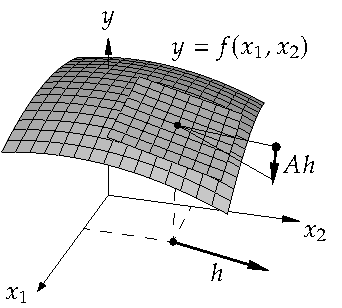
\includegraphics{figures/svder}
\caption{Illustration of a derivative for a function $f \colon \R^2 \to \R$.  The vector $h$ is shown
in the $x_1x_2$-plane based at $(x_1,x_2)$, and the vector
$Ah \in \R^1$ is shown along the $y$ direction.\label{fig:svder}}
\end{myfigureht}

For a differentiable function,
the derivative of $f$ is a function from $U$ to $L(\R^n,\R^m)$.  Compare
to the one-dimensional case, where the derivative is a function
from $U$ to $\R$, but we really want to think of $\R$ here as
$L(\R^1,\R^1)$.  As in one dimension, the idea is that a differentiable
mapping is \myquote{infinitesimally close} to a linear mapping, and this
linear mapping is the derivative.

Notice which norms are being used in the definition.
The norm in the
numerator is on $\R^m$, and the norm in the denominator is on $\R^n$ where $h$
lives.
Normally it is understood that $h \in \R^n$ from context
(the formula makes no sense otherwise).
We will not explicitly say so from now on.

We have again cheated somewhat and said that $A$
is \emph{the} derivative.  We have not shown yet that there
is only one, let us do that now.

\begin{prop}
Let $U \subset \R^n$ be an open subset and $f \colon U \to \R^m$ a function.  Suppose
$x \in U$ and there exist 
$A,B \in L(\R^n,\R^m)$ such that
\begin{equation*}
\lim_{h \to 0}
\frac{\snorm{f(x+h)-f(x) - Ah}}{\snorm{h}} = 0
\qquad \text{and} \qquad
\lim_{h \to 0}
\frac{\snorm{f(x+h)-f(x) - Bh}}{\snorm{h}} = 0 .
\end{equation*}
Then $A=B$.
\end{prop}

\begin{proof}
Suppose $h \in \R^n$, $h \not= 0$.  Compute
\begin{equation*}
\begin{split}
\frac{\snorm{(A-B)h}}{\snorm{h}} & =
\frac{\snorm{f(x+h)-f(x) - Ah - (f(x+h)-f(x) - Bh)}}{\snorm{h}} \\
& \leq
\frac{\snorm{f(x+h)-f(x) - Ah}}{\snorm{h}} + \frac{\snorm{f(x+h)-f(x) -
Bh}}{\snorm{h}} .
\end{split}
\end{equation*}
So 
$\frac{\snorm{(A-B)h}}{\snorm{h}} \to 0$ as $h \to 0$.  That is, given
$\epsilon > 0$, then for all nonzero $h$ in some $\delta$-ball around
the origin
\begin{equation*}
\epsilon > 
\frac{\snorm{(A-B)h}}{\snorm{h}}
=
\norm{(A-B)\frac{h}{\snorm{h}}} .
\end{equation*}
For any given $x$ with $\snorm{x}=1$,
let $h = (\nicefrac{\delta}{2}) \, x$, then $\snorm{h} < \delta$
and $\frac{h}{\snorm{h}} = x$.
So $\snorm{(A-B)x} < \epsilon$.  Taking the supremum over all $x$ with
$\snorm{x} = 1$, we get the operator norm
$\snorm{A-B} \leq \epsilon$.  As $\epsilon > 0$
was arbitrary, $\snorm{A-B} = 0$, or in other words $A = B$.
\end{proof}

\begin{example}
If $f(x) = Ax$ for a linear mapping $A$, then
$f'(x) = A$:
\begin{equation*}
\frac{\snorm{f(x+h)-f(x) - Ah}}{\snorm{h}}
=
\frac{\snorm{A(x+h)-Ax - Ah}}{\snorm{h}}
=
\frac{0}{\snorm{h}} = 0 .
\end{equation*}
\end{example}

\begin{example}
Let $f \colon \R^2 \to \R^2$ be defined by
\begin{equation*}
f(x,y) = \bigl(f_1(x,y),f_2(x,y)\bigr) := (1+x+2y+x^2,2x+3y+xy).
\end{equation*}
Let us show that $f$ is differentiable at the origin and let us 
compute the derivative,
directly using the definition.  If the
derivative exists, it is in $L(\R^2,\R^2)$, so it can be
represented by a $2$-by-$2$ matrix
$\left[\begin{smallmatrix}a&b\\c&d\end{smallmatrix}\right]$.  Suppose $h =
(h_1,h_2)$.  We need the following expression to go to zero.
\begin{multline*}
\frac{\snorm{
f(h_1,h_2)-f(0,0)
-
(ah_1 +bh_2 , ch_1+dh_2)}
}{\snorm{(h_1,h_2)}}
=
\\
\frac{\sqrt{
{\bigl((1-a)h_1 + (2-b)h_2 + h_1^2\bigr)}^2
+
{\bigl((2-c)h_1 + (3-d)h_2 + h_1h_2\bigr)}^2}}{\sqrt{h_1^2+h_2^2}} .
\end{multline*}
If we choose $a=1$, $b=2$, $c=2$, $d=3$, the expression becomes
\begin{equation*}
\frac{\sqrt{
h_1^4 + h_1^2h_2^2}}{\sqrt{h_1^2+h_2^2}}
=
\sabs{h_1}
\frac{\sqrt{
h_1^2 + h_2^2}}{\sqrt{h_1^2+h_2^2}}
= \sabs{h_1} .
\end{equation*}
This expression does indeed go to zero as $h \to 0$.  The
function $f$ is differentiable at the origin and 
the derivative $f'(0)$ is represented by the matrix
$\left[\begin{smallmatrix}1&2\\2&3\end{smallmatrix}\right]$.
\end{example}

\begin{prop}
Let $U \subset \R^n$ be open and $f \colon U \to \R^m$ be
differentiable at $p \in U$.  Then $f$ is continuous at $p$.
\end{prop}

\begin{proof}
Another way to write the differentiability of $f$ at $p$ is to consider
\begin{equation*}
r(h) := f(p+h)-f(p) - f'(p) h .
\end{equation*}
The function $f$ is differentiable at $p$ if
$\frac{\snorm{r(h)}}{\snorm{h}}$ goes to zero as $h \to 0$,
so
$r(h)$ itself goes to zero.  The mapping $h \mapsto f'(p) h$
is a linear mapping between finite-dimensional spaces, hence continuous
and $f'(p) h \to 0$ as $h \to 0$.  Thus,
$f(p+h)$ must go to $f(p)$ as $h \to 0$.  That is, $f$ is continuous at $p$.
\end{proof}

The derivative is itself a linear operator on the space of differentiable
functions.

\begin{prop}
Suppose $U \subset \R^n$ is open,
$f \colon U \to \R^m$ and
$g \colon U \to \R^m$ are differentiable at $p$,
and $\alpha \in \R$.  Then the functions $f+g$ and $\alpha f$
are differentiable at $p$ and
\begin{equation*}
(f+g)'(p) = f'(p) + g'(p) , \qquad \text{and} \qquad (\alpha f)'(p) = \alpha
f'(p) .
\end{equation*}
\end{prop}

\begin{proof}
Let $h \in \R^n$, $h \not= 0$.  Then
\begin{multline*}
\frac{\norm{f(p+h)+g(p+h)-\bigl(f(p)+g(p)\bigr) - \bigl(f'(p) + g'(p)\bigr)h}}{\snorm{h}}
\\
\leq
\frac{\norm{f(p+h)-f(p) - f'(p)h}}{\snorm{h}}
+
\frac{\norm{g(p+h)-g(p) - g'(p)h}}{\snorm{h}} ,
\end{multline*}
and
\begin{equation*}
\frac{\norm{\alpha f(p+h) - \alpha f(p) - \alpha f'(p)h}}{\snorm{h}}
=
\sabs{\alpha} \frac{\norm{f(p+h))-f(p) - f'(p)h}}{\snorm{h}} .
\end{equation*}
The limits as $h$ goes to zero of the right-hand sides are zero by
hypothesis.  The result follows.
\end{proof}

If $A \in L(X,Y)$ and $B \in L(Y,Z)$ are linear maps, then 
they are their own derivative.  The composition
$BA \in L(X,Z)$ is also its own derivative, and
so the derivative of the composition is the composition
of the derivatives.  As differentiable maps are
\myquote{infinitesimally close}
to linear maps, they have the same property:

\begin{thm}[Chain rule] \index{chain rule}
Let $U \subset \R^n$ be open and let $f \colon U \to \R^m$ be
differentiable at $p \in U$.  Let $V \subset \R^m$ be open,
$f(U) \subset V$ and let $g \colon V \to \R^\ell$ be differentiable
at $f(p)$.  Then
\begin{equation*}
F(x) = g\bigl(f(x)\bigr)
\end{equation*}
is differentiable at $p$ and
\begin{equation*}
F'(p) = g'\bigl(f(p)\bigr) f'(p) .
\end{equation*}
\end{thm}

Without the points where things are evaluated, this is sometimes written as
$F' = {(g \circ f)}' = g' f'$.  The way to
understand it is that the derivative of the composition $g \circ f$
is the composition of the derivatives of $g$ and $f$.  If
$f'(p) = A$ and $g'\bigl(f(p)\bigr) = B$, then $F'(p) = BA$,
just as for linear maps.

\begin{proof}
Let $A := f'(p)$ and $B := g'\bigl(f(p)\bigr)$.  Take a nonzero $h \in \R^n$
and write $q = f(p)$, $k = f(p+h)-f(p)$.  Let
\begin{equation*}
r(h) := f(p+h)-f(p) - A h . %= k - Ah.
\end{equation*}
Then $r(h) = k-Ah$ or $Ah = k-r(h)$, and $f(p+h) = q+k$.
We look at the quantity we need to go
to zero:
\begin{equation*}
\begin{split}
\frac{\snorm{F(p+h)-F(p) - BAh}}{\snorm{h}}
& =
\frac{\snorm{g\bigl(f(p+h)\bigr)-g\bigl(f(p)\bigr) - BAh}}{\snorm{h}}
\\
& =
\frac{\snorm{g(q+k)-g(q) - B\bigl(k-r(h)\bigr)}}{\snorm{h}}
\\
& \leq
\frac
{\snorm{g(q+k)-g(q) - Bk}}
{\snorm{h}}
+
\snorm{B}
\frac
{\snorm{r(h)}}
{\snorm{h}}
\\
& =
\frac
{\snorm{g(q+k)-g(q) - Bk}}
{\snorm{k}}
\frac
{\snorm{f(p+h)-f(p)}}
{\snorm{h}}
+
\snorm{B}
\frac
{\snorm{r(h)}}
{\snorm{h}} .
\end{split}
\end{equation*}
First, $\snorm{B}$ is a constant and $f$ is differentiable at $p$,
so
the term $\snorm{B}\frac{\snorm{r(h)}}{\snorm{h}}$ goes to 0.
Next because $f$ is continuous at $p$, then as
$h$ goes to 0, so $k$ goes to 0.  Thus
$\frac
{\snorm{g(q+k)-g(q) - Bk}}
{\snorm{k}}$ goes to 0, because $g$ is differentiable at $q$.
Finally,
\begin{equation*}
\frac
{\snorm{f(p+h)-f(p)}}
{\snorm{h}}
\leq
\frac
{\snorm{f(p+h)-f(p)-Ah}}
{\snorm{h}}
+
\frac
{\snorm{Ah}}
{\snorm{h}}
\leq
\frac
{\snorm{f(p+h)-f(p)-Ah}}
{\snorm{h}}
+
\snorm{A} .
\end{equation*}
As $f$ is differentiable at $p$,
for small enough $h$, the quantity
$\frac{\snorm{f(p+h)-f(p)-Ah}}{\snorm{h}}$ is bounded.  Hence, the
term
$
\frac
{\snorm{f(p+h)-f(p)}}
{\snorm{h}}
$
stays bounded as $h$ goes to 0.  Therefore, 
$\frac{\snorm{F(p+h)-F(p) - BAh}}{\snorm{h}}$ goes to zero, and
$F'(p) = BA$, which is what was claimed.
\end{proof}

\subsection{Partial derivatives}

There is another way to generalize the derivative from one dimension.
We hold all but one variable constant and take the regular
derivative.

\begin{defn}
Let
$f \colon U \to \R$ be a function on an open set $U \subset \R^n$.
If the following limit exists, we write
\glsadd{not:partialder}
\begin{equation*}
\frac{\partial f}{\partial x_j} (x) := 
\lim_{h\to 0}\frac{f(x_1,\ldots,x_{j-1},x_j+h,x_{j+1},\ldots,x_n)-f(x)}{h}
=
\lim_{h\to 0}\frac{f(x+h e_j)-f(x)}{h} .
\end{equation*}
We call 
$\frac{\partial f}{\partial x_j} (x)$ the \emph{\myindex{partial derivative}}
of $f$
with respect to $x_j$.  %Sometimes we write $D_j f$ instead.
See \figureref{fig:svpartder}.
Here $h$ is a number not a vector.

For a mapping $f \colon U \to \R^m$ we write
$f = (f_1,f_2,\ldots,f_m)$, where $f_k$ are real-valued
functions.  We then take partial derivatives of
the components,
$\frac{\partial f_k}{\partial x_j}$.
\end{defn}

\begin{myfigureht}
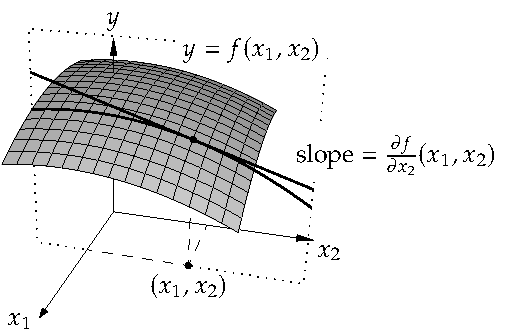
\includegraphics{figures/svpartder}
\caption{Illustration of a partial derivative for a function $f \colon \R^2
\to \R$.  The $yx_2$-plane where $x_1$ is fixed is marked in dotted line,
and the slope of the tangent line in the $yx_2$-plane is
$\frac{\partial f}{\partial x_2}(x_1,x_2)$.\label{fig:svpartder}}
\end{myfigureht}

Partial derivatives are easier to compute with all the machinery of
calculus, and they provide a way to compute the derivative of a
function.

\begin{prop} \label{mv:prop:jacobianmatrix}
Let $U \subset \R^n$ be open and let $f \colon U \to \R^m$ be
differentiable at $p \in U$.  Then all the partial derivatives at $p$
exist and, in terms of the standard bases of $\R^n$ and $\R^m$,
$f'(p)$ is represented by the matrix
\begin{equation*}
\begin{bmatrix}
\frac{\partial f_1}{\partial x_1}(p)
&
\frac{\partial f_1}{\partial x_2}(p)
& \ldots &
\frac{\partial f_1}{\partial x_n}(p)
\\[6pt]
\frac{\partial f_2}{\partial x_1}(p)
&
\frac{\partial f_2}{\partial x_2}(p)
& \ldots &
\frac{\partial f_2}{\partial x_n}(p)
\\
\vdots & \vdots & \ddots & \vdots
\\
\frac{\partial f_m}{\partial x_1}(p)
&
\frac{\partial f_m}{\partial x_2}(p)
& \ldots &
\frac{\partial f_m}{\partial x_n}(p)
\end{bmatrix} .
\end{equation*}
\end{prop}


In other words,
\begin{equation*}
f'(p) \, e_j =
\sum_{k=1}^m
\frac{\partial f_k}{\partial x_j}(p) \,e_k .
\end{equation*}
If $v = \sum_{j=1}^n c_j\, e_j = (c_1,c_2,\ldots,c_n)$, then
\begin{equation*}
f'(p) \, v =
\sum_{j=1}^n
\sum_{k=1}^m
 c_j
\frac{\partial f_k}{\partial x_j}(p) \,e_k
=
\sum_{k=1}^m
\left(
\sum_{j=1}^n
 c_j
\frac{\partial f_k}{\partial x_j}(p) \right) \,e_k .
\end{equation*}

\begin{proof}
Fix a $j$ and note that for nonzero $h$,
\begin{equation*}
\begin{split}
\norm{\frac{f(p+h e_j)-f(p)}{h} - f'(p) \, e_j} & = 
\norm{\frac{f(p+h e_j)-f(p) - f'(p) \, h e_j}{h}} \\
& =
\frac{\snorm{f(p+h e_j)-f(p) - f'(p) \, h e_j}}{\snorm{h e_j}} .
\end{split}
\end{equation*}
As $h$ goes to 0, the right-hand side goes to zero by
differentiability of $f$, and hence
\begin{equation*}
\lim_{h \to 0}
\frac{f(p+h e_j)-f(p)}{h} = f'(p) \, e_j  .
\end{equation*}
Let us represent $f$ by components
$f = (f_1,f_2,\ldots,f_m)$, since it is vector-valued.
Taking a limit in $\R^m$
is the same as taking the limit in each component separately.  
For every $k$,
the partial derivative
\begin{equation*}
\frac{\partial f_k}{\partial x_j} (p)
=
\lim_{h \to 0}
\frac{f_k(p+h e_j)-f_k(p)}{h}
\end{equation*}
exists and is equal to the $k$th component of $f'(p)\, e_j$,
and we are done.
\end{proof}

The converse of the proposition is not true.  Just because the partial
derivatives exist, does not mean that the function is differentiable.  See
the exercises.
However, when the partial derivatives are continuous, we will prove that the
converse holds.
One of the consequences of the proposition is that if $f$
is differentiable on $U$, then $f' \colon U \to
L(\R^n,\R^m)$ is a continuous function if and only if
all the $\frac{\partial f_k}{\partial x_j}$ are continuous functions.

\subsection{Gradients, curves, and directional derivatives}

Let $U \subset \R^n$ be open and $f \colon U \to \R$ a differentiable
function.  We define
the \emph{\myindex{gradient}} as
\glsadd{not:gradient}
\begin{equation*}
\nabla f (x) := \sum_{j=1}^n \frac{\partial f}{\partial x_j} (x)\, e_j .
\end{equation*}
The gradient gives a way to represent the action of
the derivative as a dot product: $f'(x)\,v = \nabla f(x) \cdot v$.

Suppose $\gamma \colon (a,b) \subset \R \to \R^n$ is a differentiable
function.
Such a function and its image is sometimes called a \emph{\myindex{curve}},
or a \emph{\myindex{differentiable curve}}.
Write $\gamma =
(\gamma_1,\gamma_2,\ldots,\gamma_n)$.
For the purposes of computation
we identify $L(\R^1)$ and $\R$ as we did when we defined the
derivative in one variable.
We also identify $L(\R^1,\R^n)$ with $\R^n$.
We treat $\gamma^{\:\prime}(t)$ both as an operator in
$L(\R^1,\R^n)$ and the vector
$\bigl(\gamma_1^{\:\prime}(t),
\gamma_2^{\:\prime}(t),\ldots,\gamma_n^{\:\prime}(t)\bigr)$
in $\R^n$.
Using \propref{mv:prop:jacobianmatrix},
if $v\in \R^n$ is $\gamma^{\:\prime}(t)$ acting as a vector,
then $h \mapsto h \, v$ (for $h \in \R^1 = \R$) is
$\gamma^{\:\prime}(t)$ acting as an operator
in $L(\R^1,\R^n)$.
We often use this 
slight abuse of notation when dealing with curves.
See \figureref{fig:difcurveder}.
\begin{myfigureht}
\subimport*{figures/}{diffcurveder.pdf_t}
\caption{Differentiable curve and its derivative as a
vector.\label{fig:difcurveder}}
\end{myfigureht}

Suppose $\gamma\bigl((a,b)\bigr) \subset U$ and let
\begin{equation*}
g(t) := f\bigl(\gamma(t)\bigr) .
\end{equation*}
The function
$g$ is differentiable. Treating $g'(t)$ as a number,
\begin{equation*}
g'(t) =
f'\bigl(\gamma(t)\bigr) \gamma^{\:\prime}(t)
=
\sum_{j=1}^n
\frac{\partial f}{\partial x_j} \bigl(\gamma(t)\bigr)
\frac{d\gamma_j}{dt} (t)
=
\sum_{j=1}^n
\frac{\partial f}{\partial x_j}
\frac{d\gamma_j}{dt} .
\end{equation*}
For convenience,
we often 
leave out the points where we are evaluating,
such as above on the far right-hand side.
With the notation of the gradient and the dot product
the equation becomes
\begin{equation*}
g'(t) = (\nabla f) \bigl(\gamma(t)\bigr) \cdot \gamma^{\:\prime}(t)
= \nabla f \cdot \gamma^{\:\prime}.
\end{equation*}

We use this idea to define derivatives in a specific direction.  A direction
is simply a vector pointing in that direction.  Pick a vector $u \in \R^n$
such that $\snorm{u} = 1$, and fix $x \in U$.
We define the
\emph{\myindex{directional derivative}} as
\glsadd{not:mvdirder}
\begin{equation*}
D_u f (x) := \frac{d}{dt}\Big|_{t=0} \bigl[ f(x+tu) \bigr] =
\lim_{h\to 0}
\frac{f(x+hu)-f(x)}{h} ,
\end{equation*}
where the notation
$\frac{d}{dt}\big|_{t=0}$ represents the derivative evaluated at $t=0$.
Taking the standard basis vector $e_j$ we find
$\frac{\partial f}{\partial x_j} = D_{e_j} f$.
For this reason, sometimes the notation $\frac{\partial f}{\partial u}$
is used instead of $D_u f$.

Let $\gamma$ be defined by
\begin{equation*}
\gamma(t) := x + tu .
\end{equation*}
Then $\gamma^{\:\prime}(t) = u$ for all $t$.  
By the computation above:
\begin{equation*}
D_u f (x) =
\frac{d}{dt}\Big|_{t=0} \bigl[ f(x+tu) \bigr] =
(\nabla f) \bigl(\gamma(0)\bigr) \cdot \gamma^{\:\prime}(0)
=
(\nabla f) (x) \cdot u .
\end{equation*}

Suppose $(\nabla f)(x) \neq 0$.
By the Cauchy--Schwarz inequality,
\begin{equation*}
\sabs{D_u f(x)} \leq \snorm{(\nabla f)(x)} .
\end{equation*}
Equality is achieved when $u$ is a scalar multiple of
$(\nabla f)(x)$.  That is, when
\begin{equation*}
u = 
\frac{(\nabla f)(x)}{\snorm{(\nabla f)(x)}} ,
\end{equation*}
we get $D_u f(x) = \snorm{(\nabla f)(x)}$.
The gradient points in the direction in which the
function grows fastest, in other words,
in the direction in which $D_u f(x)$ is maximal.

\subsection{The Jacobian}

\begin{defn}
Let $U \subset \R^n$ and
$f \colon U \to \R^n$ be a differentiable mapping.  Define the
\emph{\myindex{Jacobian}}%
\footnote{Named after the Italian mathematician
\href{https://en.wikipedia.org/wiki/Carl_Gustav_Jacob_Jacobi}{Carl Gustav Jacob Jacobi}
(1804--1851).},
or the
\emph{\myindex{Jacobian determinant}}%
\footnote{The matrix from \propref{mv:prop:jacobianmatrix} representing $f'(x)$
is sometimes called the
\emph{\myindex{Jacobian matrix}}.},
of $f$ at $x$ as
\glsadd{not:jacobdet}
\begin{equation*}
J_f(x) := \det\bigl( f'(x) \bigr) .
\end{equation*}
Sometimes $J_f$ is written as
\begin{equation*}
\frac{\partial(f_1,f_2,\ldots,f_n)}{\partial(x_1,x_2,\ldots,x_n)} .
\end{equation*}
\end{defn}

This last piece of notation may seem somewhat confusing,
but it is quite useful when we need to specify
the exact variables and function components used,
as will for example do in the implicit function theorem.

The Jacobian $J_f$ is a real-valued function, and when $n=1$ it is simply the
derivative.
From the chain rule and the fact that $\det(AB) = \det(A)\det(B)$, it follows that:
\begin{equation*}
J_{f \circ g} (x) = J_f\bigl(g(x)\bigr) J_g(x) .
\end{equation*}

The determinant of a linear mapping tells us what happens to
area/volume under the mapping.
Similarly, the Jacobian measures how much a differentiable mapping stretches
things locally, and if it flips orientation.  In particular, if the Jacobian
is non-zero than we would assume that locally the mapping is invertible (and
we would be correct as we will later see).

\subsection{Exercises}

\begin{exercise}
Suppose $\gamma \colon (-1,1) \to \R^n$ and
$\alpha \colon (-1,1) \to \R^n$ are two differentiable curves
such that $\gamma(0) = \alpha(0)$ and $\gamma^{\:\prime}(0) = \alpha'(0)$.
Suppose $F \colon \R^n \to \R$ is a differentiable function.  Show that
\begin{equation*}
\frac{d}{dt}\Big|_{t=0}
F\bigl(\gamma(t)\bigr)
=
\frac{d}{dt}\Big|_{t=0}
F\bigl(\alpha(t)\bigr)
.
\end{equation*}
\end{exercise}

\begin{exercise}
Let $f \colon \R^2 \to \R$ be given by
$f(x,y)
:=
\sqrt{x^2+y^2}$,
see \figureref{fig:distfromorgfunc}.
Show that $f$ is not differentiable at the origin.
\end{exercise}

\begin{myfigureht}
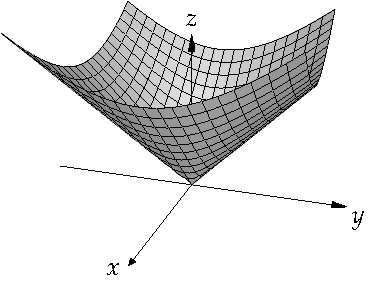
\includegraphics{figures/distfromorgfunc}
\caption{Graph of $\sqrt{x^2+y^2}$.\label{fig:distfromorgfunc}}
\end{myfigureht}

\begin{samepage}
\begin{exercise}
Using only the definition of the derivative, show that
the following $f \colon \R^2 \to \R^2$ are differentiable at the origin and
find their derivative.
\begin{enumerate}[a)]
\item
$f(x,y) := (1+x+xy,x)$,
\item
$f(x,y) := \bigl(y-y^{10},x \bigr)$,
\item
$f(x,y) := \bigl( {(x+y+1)}^2 , {(x-y+2)}^2 \bigr)$.
\end{enumerate}
\end{exercise}
\end{samepage}

\begin{exercise}
Suppose $f \colon \R \to \R$ and $g \colon \R \to \R$ are differentiable
functions.  Using only the definition of the derivative, show that
$h \colon \R^2 \to \R^2$ defined by $h(x,y)
:= \bigl(f(x),g(y)\bigr)$ is a differentiable function, and find the
derivative, at all points $(x,y)$.
\end{exercise}

\begin{exercise} \label{exercise:noncontpartialsexist}
Define a function $f \colon \R^2 \to \R$ by
(see \figureref{fig:xyxsqysqvol2})
\begin{equation*}
f(x,y)
:=
\begin{cases}
\frac{xy}{x^2+y^2} & \text{if } (x,y) \not= (0,0), \\
0                  & \text{if } (x,y) = (0,0).
\end{cases}
\end{equation*}
\begin{enumerate}[a)]
\item
Show that the partial derivatives 
$\frac{\partial f}{\partial x}$ and
$\frac{\partial f}{\partial y}$ exist at all points (including the origin).
\item
Show that $f$ is not continuous at the origin (and hence not
differentiable).
\end{enumerate}
\end{exercise}

\begin{myfigureht}
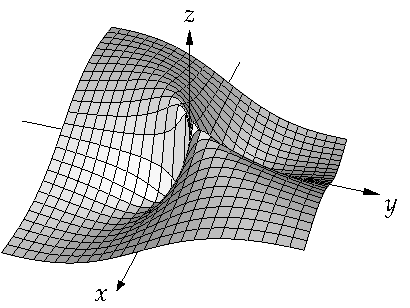
\includegraphics{figures/xyxsqysq}
\caption{Graph of $\frac{xy}{x^2+y^2}$.\label{fig:xyxsqysqvol2}}
\end{myfigureht}

\begin{samepage}
\begin{exercise}
Define a function $f \colon \R^2 \to \R$ by
(see \figureref{fig:xsqyxsqysq})
\begin{equation*}
f(x,y)
:=
\begin{cases}
\frac{x^2y}{x^2+y^2} & \text{if } (x,y) \not= (0,0), \\
0                    & \text{if } (x,y) = (0,0).
\end{cases}
\end{equation*}
\begin{enumerate}[a)]
\item
Show that the partial derivatives 
$\frac{\partial f}{\partial x}$ and
$\frac{\partial f}{\partial y}$ exist at all points.
\item
Show that for all $u \in \R^2$ with $\snorm{u}=1$, the directional
derivative $D_u f$ exists at all points.
\item
Show that $f$ is continuous at the origin.
\item
Show that $f$ is not differentiable at the origin.
\end{enumerate}
\end{exercise}
\end{samepage}

\begin{myfigureht}
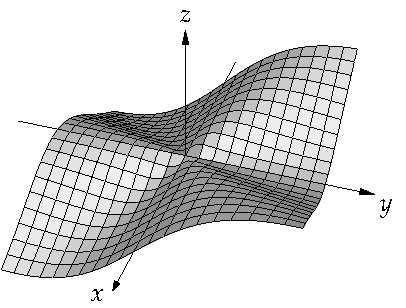
\includegraphics{figures/xsqyxsqysq}
\caption{Graph of $\frac{x^2y}{x^2+y^2}$.\label{fig:xsqyxsqysq}}
\end{myfigureht}

\begin{samepage}
\begin{exercise}
Suppose $f \colon \R^n \to \R^n$ is one-to-one, onto, differentiable at all
points, and such that $f^{-1}$ is also differentiable at all points.
\begin{enumerate}[a)]
\item
Show that $f'(p)$ is invertible at all points $p$ and compute
${(f^{-1})}'\bigl(f(p)\bigr)$.  Hint: Consider $x = f^{-1}\bigl(f(x)\bigr)$.
\item
Let $g \colon \R^n \to \R^n$ be a function differentiable at $q \in \R^n$
and such that $g(q)=q$.  Suppose $f(p) = q$ for some $p \in \R^n$.
Show $J_g(q) = J_{f^{-1} \circ g \circ f}(p)$ where $J_g$ is the Jacobian
determinant.
\end{enumerate}
\end{exercise}
\end{samepage}

\begin{exercise}
Suppose $f \colon \R^2 \to \R$ is differentiable and such that
$f(x,y) = 0$ if and only if $y=0$ and such that $\nabla f(0,0) = (0,1)$.
Prove that $f(x,y) > 0$ whenever $y > 0$, and
$f(x,y) < 0$ whenever $y < 0$.
\end{exercise}

\pagebreak[2]
\begin{exnote}
As for functions of one variable, $f \colon U \to \R$ has a
\emph{\myindex{relative maximum}} at $p \in U$ if there exists
a $\delta >0$ such that $f(q) \leq f(p)$ for all $q \in B(p,\delta) \cap U$.
Similarly for \emph{\myindex{relative minimum}}.
\end{exnote}

\begin{exercise} \label{exercise:mv:maximumcritical}
Suppose $U \subset \R^n$ is open and
$f \colon U \to \R$ is differentiable.  Suppose $f$ has a relative maximum
at $p \in U$.  Show that $f'(p) = 0$, that is the zero mapping in
$L(\R^n,\R)$.  That is $p$ is a
\emph{\myindex{critical point}} of $f$.
\end{exercise}

\begin{exercise}
Suppose $f \colon \R^2 \to \R$ is differentiable and 
$f(x,y) = 0$ whenever $x^2+y^2 = 1$.
Prove that there exists at least
one point $(x_0,y_0)$ such that
$\frac{\partial f}{\partial x}(x_0,y_0) = \frac{\partial f}{\partial
y}(x_0,y_0) = 0$.
\end{exercise}

\begin{exercise} \label{exercise:peano}
Define $f(x,y) := ( x-y^2 ) ( 2 y^2 - x)$.  The graph of $f$ is called
the \emph{\myindex{Peano surface}}.%
\footnote{Named after the Italian mathematician
\href{https://en.wikipedia.org/wiki/Giuseppe_Peano}{Giuseppe Peano}
(1858--1932).}
\begin{enumerate}[a)]
\item
Show that
$(0,0)$ is a critical point, that is $f'(0,0) = 0$, that is the zero
linear map in $L(\R^2,\R)$.
\item
Show that for every direction the restriction of $f$ to a line through the origin
in that direction has a relative maximum at the origin.  In other words,
for every $(x,y)$ such that $x^2+y^2=1$, the function $g(t) := f(tx,ty)$,
has a relative maximum at $t=0$.\\
Hint: While not necessary
\volIref{\sectionref*{vI-sec:taylor} of volume I}{\sectionref{sec:taylor}}
makes
this part easier.
\item
Show that $f$ does not have a relative maximum at $(0,0)$.
\end{enumerate}
\end{exercise}

\begin{exercise}
Suppose $f \colon \R \to \R^n$ is differentiable and $\snorm{f(t)} = 1$ for
all $t$ (that is, we have a curve in the unit sphere).  Show that 
$f'(t) \cdot f(t) = 0$ (treating $f'$ as a vector) for all $t$.
\end{exercise}

\begin{exercise}
Define $f \colon \R^2 \to \R^2$ by $f(x,y) :=
\bigl(x,y+\varphi(x)\bigr)$ for some differentiable function $\varphi$ of one
variable.  Show $f$ is differentiable and find $f'$.
\end{exercise}

\begin{exercise}
Suppose $U \subset \R^n$ is open, $p \in U$, and
$f \colon U \to \R$,
$g \colon U \to \R$,
$h \colon U \to \R$ are functions such that
$f(p) = g(p) = h(p)$, $f$ and $h$ are differentiable at $p$,
$f'(p) = h'(p)$, and
\begin{equation*}
f(x) \leq g(x) \leq h(x)
\end{equation*}
for all $x \in U$.  Show that $g$ is differentiable at $p$ and 
$g'(p) = f'(p) = h'(p)$.
\end{exercise}

%%%%%%%%%%%%%%%%%%%%%%%%%%%%%%%%%%%%%%%%%%%%%%%%%%%%%%%%%%%%%%%%%%%%%%%%%%%%%%

\sectionnewpage
\section{Continuity and the derivative}
\label{sec:svthedercont}

\sectionnotes{1--2 lectures}

\subsection{Bounding the derivative}

Let us prove a \myquote{mean value theorem} for vector-valued functions.

\begin{lemma} \label{lemma:mvtmv}
If $\varphi \colon [a,b] \to \R^n$ is differentiable on $(a,b)$ and
continuous on $[a,b]$, then there exists a $t_0 \in (a,b)$ such that
\begin{equation*}
\snorm{\varphi(b)-\varphi(a)} \leq (b-a) \snorm{\varphi'(t_0)} .
\end{equation*}
\end{lemma}

\begin{proof}
By the mean value theorem on the scalar-valued function
$t \mapsto \bigl(\varphi(b)-\varphi(a) \bigr) \cdot \varphi(t)$,
where the dot is the dot product, we obtain
that
there is a $t_0 \in (a,b)$ such that
\begin{equation*}
\begin{split}
\snorm{\varphi(b)-\varphi(a)}^2
& =
\bigl( \varphi(b)-\varphi(a) \bigr)
\cdot
\bigl( \varphi(b)-\varphi(a) \bigr)
\\
& =
\bigl(\varphi(b)-\varphi(a) \bigr) \cdot \varphi(b) - 
\bigl(\varphi(b)-\varphi(a) \bigr) \cdot \varphi(a)
\\
& = 
(b-a)
\bigl(\varphi(b)-\varphi(a) \bigr) \cdot \varphi'(t_0) ,
\end{split}
\end{equation*}
where we treat $\varphi'$ as a vector in $\R^n$ by the abuse of
notation we mentioned in the previous section.
If we think of $\varphi'(t)$ as a vector, then by
\exerciseref{exercise:normonedim},
$\snorm{\varphi'(t)}_{L(\R,\R^n)} = \snorm{\varphi'(t)}_{\R^n}$.
That is, the euclidean norm of the vector is the same as the operator norm
of $\varphi'(t)$.

By the Cauchy--Schwarz inequality
\begin{equation*}
\snorm{\varphi(b)-\varphi(a)}^2
=
(b-a)\bigl(\varphi(b)-\varphi(a) \bigr) \cdot \varphi'(t_0)
\leq
(b-a)
\snorm{\varphi(b)-\varphi(a)} \, \snorm{\varphi'(t_0)} . \qedhere
\end{equation*}
\end{proof}

Recall that a set $U$ is convex
if whenever $x,y \in U$, the line segment from
$x$ to $y$ lies in $U$.

\begin{prop} \label{mv:prop:convexlip}
Let $U \subset \R^n$ be a convex open set, $f \colon U \to \R^m$
be a differentiable function, and an $M$ be such that
\begin{equation*}
\snorm{f'(x)} \leq M
\qquad \text{for all } x \in U.
\end{equation*}
Then $f$ is Lipschitz with constant $M$, that is
\begin{equation*}
\snorm{f(x)-f(y)} \leq M \snorm{x-y}
\qquad
\text{for all } x,y \in U.
\end{equation*}
\end{prop}

\begin{proof}
Fix $x$ and $y$ in $U$ and note that
$(1-t)x+ty \in U$ for all $t \in [0,1]$
by convexity.
Next
\begin{equation*}
\frac{d}{dt} \Bigl[f\bigl((1-t)x+ty\bigr)\Bigr]
=
f'\bigl((1-t)x+ty\bigr) (y-x) .
\end{equation*}
By \lemmaref{lemma:mvtmv} there is some
$t_0 \in (0,1)$ such that
\begin{equation*}
\begin{split}
\snorm{f(x)-f(y)} & \leq
\norm{\frac{d}{dt} \Big|_{t=t_0} \Bigl[ f\bigl((1-t)x+ty\bigr) \Bigr] }
\\
& \leq
\norm{f'\bigl((1-t_0)x+t_0y\bigr)} \, \snorm{y-x} \leq
M \snorm{y-x} . \qedhere
\end{split}
\end{equation*}
\end{proof}

\begin{example}
If $U$ is not convex the proposition is not true: Consider
the set
\begin{equation*}
U := \bigl\{ (x,y) : 0.5 < x^2+y^2 < 2 \bigr\} \setminus \bigl\{ (x,0) : x <
0 \bigr\} .
\end{equation*}
For $(x,y) \in U$,
let $f(x,y)$ be the angle that the line from the origin to $(x,y)$
makes with the positive $x$ axis.  We even have a formula for $f$:
\begin{equation*}
f(x,y) = 2 \operatorname{arctan}\left( \frac{y}{x+\sqrt{x^2+y^2}}\right) .
\end{equation*}
Think a spiral staircase with room in the middle.  See
\figureref{mv:fignonlip}.

\begin{myfigureht}
\subimport*{figures/}{nonlip_full.pdf_t}
\caption{A non-Lipschitz function with uniformly bounded
derivative.\label{mv:fignonlip}}
\end{myfigureht}

The function is differentiable,
and the derivative is bounded on $U$, which is not hard to see.   Now
think of
what happens near where the negative $x$-axis cuts the annulus in half.
As we approach this cut from positive $y$, $f(x,y)$ approaches $\pi$.
From negative $y$, $f(x,y)$ approaches $-\pi$.
So for small $\epsilon > 0$, $\sabs{f(-1,\epsilon)-f(-1,-\epsilon)}$
approaches $2\pi$, but $\snorm{(-1,\epsilon)-(-1,-\epsilon)} = 2\epsilon$,
which is arbitrarily small.  The conclusion of the proposition does not
hold for this nonconvex $U$.
\end{example}

Let us solve the differential equation $f' = 0$.

\begin{cor}
If $U \subset \R^n$ is open and connected, $f \colon U \to \R^m$ is
differentiable,
and $f'(x) = 0$ for all $x \in U$, then $f$ is constant.
\end{cor}

\begin{proof}
For any given $x \in U$, there is a ball $B(x,\delta) \subset U$.  The ball
$B(x,\delta)$ is convex.  Since
$\snorm{f'(y)} \leq 0$ for all $y \in B(x,\delta)$, then by the proposition,
$\snorm{f(x)-f(y)} \leq 0 \snorm{x-y} = 0$.  So $f(x) = f(y)$ for all $y \in
B(x,\delta)$.

This means that $f^{-1}(c)$ is open for all $c \in \R^m$.  Suppose
$f^{-1}(c)$ is nonempty.  
The two sets
\begin{equation*}
U' = f^{-1}(c), \qquad U'' = f^{-1}\bigl(\R^m\setminus\{c\}\bigr)
\end{equation*}
are open and disjoint, and further $U = U' \cup U''$.  As $U'$ is nonempty
and $U$ is connected, then
$U'' = \emptyset$.  So $f(x) = c$ for all $x \in U$.
\end{proof}

\subsection{Continuously differentiable functions}

\begin{defn}
Let $U \subset \R^n$ be open.
We say $f \colon U \to \R^m$ is
\emph{\myindex{continuously differentiable}},
or $C^1(U)$\glsadd{not:C1},
if $f$ is differentiable and $f' \colon U \to L(\R^n,\R^m)$
is continuous.
\end{defn}

\begin{prop} \label{mv:prop:contdiffpartials}
Let $U \subset \R^n$ be open and
$f \colon U \to \R^m$.  The function
$f$ is continuously differentiable if and only if 
the partial derivatives $\frac{\partial f_j}{\partial x_\ell}$
exist for all $j$ and $\ell$ and are continuous.
\end{prop}

Without continuity the theorem does not hold.  Just because
partial derivatives exist does not mean that $f$ is differentiable,
in fact, $f$ may not even be continuous.  See the exercises
for the last section and also for this section.

\begin{proof}
We proved that if $f$ is differentiable, then
the partial derivatives exist.  The partial
derivatives are the entries of the matrix of $f'(x)$.  If
$f' \colon U \to L(\R^n,\R^m)$ is continuous, then the entries are
continuous, and hence the partial derivatives are continuous.

To prove the opposite direction,
suppose the partial derivatives exist and are continuous.
Fix $x \in U$.  If we show that $f'(x)$ exists we are done, because
the entries of the matrix $f'(x)$ are the partial derivatives and if
the entries are continuous functions, the matrix-valued function $f'$ is
continuous.

We do induction on dimension.  First,
the conclusion is true when $n=1$.  In this case the derivative
is just the regular derivative (exercise, noting
that $f$ is vector-valued).

Suppose the conclusion is true for $\R^{n-1}$,
that is,
if we restrict to the first $n-1$ variables, the function is differentiable.
It is easy to see that the first $n-1$
partial derivatives of $f$ restricted to the set where the last coordinate is
fixed are the same as those for $f$.
In the following, by a slight abuse of notation,
we think of $\R^{n-1}$ as a subset of $\R^n$, that is the set in $\R^n$ where $x_n = 0$.
In other words, we identify the vectors $(x_1,x_2,\ldots,x_{n-1})$ and
$(x_1,x_2,\ldots,x_{n-1},0)$.
Let
\begin{equation*}
A := 
\begin{bmatrix}
\frac{\partial f_1}{\partial x_1}(x)
& \ldots &
\frac{\partial f_1}{\partial x_n}(x)
\\
\vdots & \ddots & \vdots
\\
\frac{\partial f_m}{\partial x_1}(x)
& \ldots &
\frac{\partial f_m}{\partial x_n}(x)
\end{bmatrix} ,
\qquad
A' := 
\begin{bmatrix}
\frac{\partial f_1}{\partial x_1}(x)
& \ldots &
\frac{\partial f_1}{\partial x_{n-1}}(x)
\\
\vdots & \ddots & \vdots
\\
\frac{\partial f_m}{\partial x_1}(x)
& \ldots &
\frac{\partial f_m}{\partial x_{n-1}}(x)
\end{bmatrix} ,
\qquad
v := 
\begin{bmatrix}
\frac{\partial f_1}{\partial x_n}(x)
\\
\vdots
\\
\frac{\partial f_m}{\partial x_n}(x)
\end{bmatrix} .
\end{equation*}
Let $\epsilon > 0$ be given.  By the induction hypothesis, there
is a $\delta > 0$ such that
for every $k \in \R^{n-1}$ with $\snorm{k} < \delta$, we have
\begin{equation*}
\frac{\snorm{f(x+k) - f(x) - A' k}}{\snorm{k}} < \epsilon .
\end{equation*}
By continuity of the partial derivatives, suppose $\delta$ is small
enough so that
\begin{equation*}
\abs{\frac{\partial f_j}{\partial x_n}(x+h)
      - \frac{\partial f_j}{\partial x_n}(x)} < \epsilon
\end{equation*}
for all $j$ and all $h \in \R^n$ with $\snorm{h} < \delta$.

Suppose $h = k + t e_n$ is a vector in $\R^n$, where $k \in \R^{n-1}$, $t
\in \R$, such that
$\snorm{h} < \delta$.  Then $\snorm{k} \leq \snorm{h} < \delta$.
Note that $Ah = A' k + tv$.
\begin{equation*}
\begin{split}
\snorm{f(x+h) - f(x) - Ah}
& = \snorm{f(x+k + t e_n) - f(x+k) - tv + f(x+k) - f(x) - A' k}
\\
& \leq \snorm{f(x+k + t e_n) - f(x+k) -tv} + \snorm{f(x+k) - f(x) -
A' k}
\\
& \leq \snorm{f(x+k + t e_n) - f(x+k) -tv} + \epsilon \snorm{k} .
\end{split}
\end{equation*}
As all the partial derivatives exist, by the mean value theorem,
for each $j$ there is some $\theta_j \in [0,t]$ (or $[t,0]$ if $t < 0$), such that
\begin{equation*}
f_j(x+k + t e_n) - f_j(x+k) =
t \frac{\partial f_j}{\partial x_n}(x+k+\theta_j e_n).
\end{equation*}
Note that if $\snorm{h} < \delta$, then $\snorm{k+\theta_j e_n} \leq \snorm{h}
< \delta$.
We finish the estimate
\begin{equation*}
\begin{split}
\snorm{f(x+h) - f(x) - Ah}
& \leq \snorm{f(x+k + t e_n) - f(x+k) -tv} + \epsilon \snorm{k}
\\
& \leq \sqrt{\sum_{j=1}^m {\left(t\frac{\partial f_j}{\partial
x_n}(x+k+\theta_j e_n) -
t \frac{\partial f_j}{\partial x_n}(x)\right)}^2} + \epsilon \snorm{k}
\\
& \leq \sqrt{m}\, \epsilon \sabs{t} + \epsilon \snorm{k}
\\
& \leq (\sqrt{m}+1)\epsilon \snorm{h} . \qedhere
\end{split}
\end{equation*}
\end{proof}

A common application is to prove that a certain function is
differentiable.  For example, let us show that all polynomials
are differentiable, and in fact continuously differentiable
by computing the partial derivatives.

\begin{cor}
A polynomial $p \colon \R^n \to \R$ in several variables
\begin{equation*}
p(x_1,x_2,\ldots,x_n)
=
\sum_{0 \leq j_1+j_2+\cdots+j_n \leq d}
c_{j_1,j_2,\ldots,j_n}
\,
x_1^{j_1}
x_2^{j_2}
\cdots
x_n^{j_n}
\end{equation*}
is continuously differentiable.
\end{cor}

\begin{proof}
Consider the partial derivative of $p$ in the $x_n$ variable.
Write $p$ as
\begin{equation*}
p(x) = \sum_{j=0}^d p_j(x_1,\ldots,x_{n-1}) \, x_n^j ,
\end{equation*}
where $p_j$ are polynomials in one less variable.
Then
\begin{equation*}
\frac{\partial p}{\partial x_n}(x)
= \sum_{j=1}^d p_j(x_1,\ldots,x_{n-1}) \, j x_n^{j-1} ,
\end{equation*}
which is again a polynomial.
So the partial derivatives of polynomials exist and are again polynomials.
By the continuity of algebraic operations, polynomials are continuous functions.
Therefore $p$ is continuously differentiable.
\end{proof}

\subsection{Exercises}

\begin{exercise}
Define $f \colon \R^2 \to \R$ as
\begin{equation*}
f(x,y) :=
\begin{cases}
(x^2+y^2)\sin\bigl({(x^2+y^2)}^{-1}\bigr) & \text{if } (x,y) \not= (0,0), \\
0                                         & \text{if } (x,y) = (0,0).
\end{cases}
\end{equation*}
Show that $f$ is differentiable at the origin, but that it is not 
continuously differentiable.
\\
Note: Feel free to use what you know about sine and cosine from calculus.
\end{exercise}

\begin{exercise}
Let $f \colon \R^2 \to \R$ be the function from
\exerciseref{exercise:noncontpartialsexist}, that is,
\begin{equation*}
f(x,y)
:=
\begin{cases}
\frac{xy}{x^2+y^2} & \text{if } (x,y) \not= (0,0), \\
0                  & \text{if } (x,y) = (0,0).
\end{cases}
\end{equation*}
Compute the partial derivatives 
$\frac{\partial f}{\partial x}$ and
$\frac{\partial f}{\partial y}$ at all points and show that these are not
continuous functions.
\end{exercise}

\begin{exercise}
Let $B(0,1) \subset \R^2$ be the unit ball (disc), that is, the set given by
$x^2 + y^2 < 1$.
Suppose $f \colon B(0,1) \to \R$ is a differentiable function
such that $\sabs{f(0,0)} \leq 1$,
and 
$\babs{\frac{\partial f}{\partial x}} \leq 1$ and
$\babs{\frac{\partial f}{\partial y}} \leq 1$ for all
points in $B(0,1)$.
\begin{enumerate}[a)]
\item
Find an $M \in \R$ such that $\snorm{f'(x,y)} \leq M$
for all $(x,y) \in
B(0,1)$.
\item
Find a $B \in \R$ such that
$\sabs{f(x,y)} \leq B$
for all $(x,y) \in
B(0,1)$.
\end{enumerate}
\end{exercise}

\begin{exercise}
Define $\varphi \colon [0,2\pi] \to \R^2$ by $\varphi(t) =
\bigl(\sin(t),\cos(t)\bigr)$.  Compute $\varphi'(t)$ for all $t$.  Compute
$\snorm{\varphi'(t)}$ for all $t$.  Notice that $\varphi'(t)$ is never zero,
yet $\varphi(0) = \varphi(2\pi)$, therefore, Rolle's theorem is not true
in more than one dimension.
\end{exercise}

\begin{exercise}
Let $f \colon \R^2 \to \R$ be a function such that
$\frac{\partial f}{\partial x}$ and
$\frac{\partial f}{\partial y}$ exist at all points and there exists an $M
\in \R$
such that 
$\babs{\frac{\partial f}{\partial x}} \leq M$ and
$\babs{\frac{\partial f}{\partial y}} \leq M$ at all points.  Show that $f$
is continuous.
\end{exercise}

\begin{samepage}
\begin{exercise}
Let $f \colon \R^2 \to \R$ be a function and
$M \in R$, such that
for every $(x,y) \in \R^2$, the function $g(t) := f(xt,yt)$ is
differentiable
and $\sabs{g'(t)} \leq M$.
\begin{enumerate}[a)]
\item
Show that $f$ is continuous at $(0,0)$.
\item
Find an example of such an $f$ that is discontinuous at every other point of
$\R^2$.\\
Hint: Think back to how we constructed a nowhere continuous function on $[0,1]$.
\end{enumerate}
\end{exercise}
\end{samepage}

\begin{exercise}
Suppose $r \colon \R^n \setminus X \to \R$ is a rational function, that is,
let $p \colon \R^n \to \R$ and
$q \colon \R^n \to \R$ be polynomials,
$q$ not identically zero,
where $X = q^{-1}(0)$, and
$r = \frac{p}{q}$.
Show that $r$ is continuously differentiable.
\end{exercise}

\begin{exercise}
Suppose $f \colon \R^n \to \R$ and $h \colon \R^n \to \R$ are two 
differentiable functions such that $f'(x) = h'(x)$ for all $x \in \R^n$.
Prove that
if $f(0) = h(0)$, then $f(x) = h(x)$ for all $x \in \R^n$.
\end{exercise}

\begin{exercise}
Prove the base case
in \propref{mv:prop:contdiffpartials}.  That is, prove that
if $n=1$ and 
\myquote{the partials exist and are continuous,} then the function is continuously
differentiable.  Note that $f$ is vector-valued.
\end{exercise}

\begin{exercise}
Suppose $g \colon \R \to \R$ is continuously differentiable and
$h \colon \R^2 \to \R$ is continuous.  Show that
\begin{equation*}
F(x,y) := g(x) + \int_0^y h(x,s) ~ds
\end{equation*}
is continuously differentiable, and that it is the solution of 
the partial differential equation $\frac{\partial F}{\partial y} = h$,
with the initial condition $F(x,0) = g(x)$ for all $x \in \R$.
\end{exercise}


%%%%%%%%%%%%%%%%%%%%%%%%%%%%%%%%%%%%%%%%%%%%%%%%%%%%%%%%%%%%%%%%%%%%%%%%%%%%%%

\sectionnewpage
\section{Inverse and implicit function theorems}
\label{sec:svinvfuncthm}

\sectionnotes{2--3 lectures}

To prove the inverse function theorem we use the contraction mapping
principle from
\volIref{\chapterref*{vI-ms:chapter}}{\chapterref{ms:chapter}},
where we we used it
to prove Picard's theorem.
Recall that a mapping $f \colon X \to Y$ between two metric
spaces $(X,d_X)$ and $(Y,d_Y)$ is called a contraction 
if there exists a $k < 1$ such that
\begin{equation*}
d_Y\bigl(f(p),f(q)\bigr) \leq k \, d_X(p,q)
\qquad \text{for all } p,q \in X.
\end{equation*}
The contraction mapping principle says that if $f \colon X \to X$
is a contraction and $X$ is a complete metric space,
then there exists a unique fixed point, that is,
there exists a unique $x \in X$ such that $f(x) = x$.

Intuitively, if a function is continuously differentiable, then it
locally \myquote{behaves like} the derivative (which is a linear function).
The idea of the inverse function theorem is that if a function is
continuously differentiable and the derivative is invertible, the function is
(locally) invertible.


\begin{thm}[Inverse function theorem]\index{inverse function theorem}
\label{thm:inverse}
Let $U \subset \R^n$ be an open set and let
$f \colon U \to \R^n$ be a continuously differentiable function.
Suppose $p \in U$ and $f'(p)$ is invertible
(that is, $J_f(p) \not=0$).
Then there exist open sets $V, W \subset \R^n$ such that
$p \in V \subset U$, $f(V) = W$ and $f|_V$ is one-to-one.  
Hence a function $g \colon W \to V$ exists such that
$g(y) := (f|_V)^{-1}(y)$.
See \figureref{fig:inversefuncRn}.
Furthermore, $g$ is continuously differentiable
and 
\begin{equation*}
g'(y) = {\bigl(f'(x)\bigr)}^{-1}, \qquad \text{for all } x \in V, y = f(x).
\end{equation*}
\end{thm}

\begin{myfigureht}
\subimport*{figures/}{inversefuncRn.pdf_t}
\caption{Setup of the inverse function theorem in $\R^n$.\label{fig:inversefuncRn}}
\end{myfigureht}

\begin{proof}
Write $A = f'(p)$.  As $f'$ is continuous, there exists an open ball
$V$ around $p$ such that
\begin{equation*}
\snorm{A-f'(x)} < \frac{1}{2\snorm{A^{-1}}}
\qquad \text{for all } x \in V.
\end{equation*}
Consequently, the derivative $f'(x)$ is invertible for all $x \in V$
by \propref{prop:finitedimpropinv}.

Given $y \in \R^n$, we define $\varphi_y \colon V \to \R^n$ by
\begin{equation*}
\varphi_y (x) := x + A^{-1}\bigl(y-f(x)\bigr) .
\end{equation*}
As $A^{-1}$ is one-to-one,
$\varphi_y(x) = x$ ($x$ is a fixed point) if only if
$y-f(x) = 0$, or in other words $f(x)=y$.  Using the chain rule we obtain
\begin{equation*}
\varphi_y'(x) = I - A^{-1} f'(x) = A^{-1} \bigl( A-f'(x) \bigr) .
\end{equation*}
So for $x \in V$, we have
\begin{equation*}
\snorm{\varphi_y'(x)} \leq \snorm{A^{-1}} \, \snorm{A-f'(x)} < \nicefrac{1}{2} .
\end{equation*}
As $V$ is a ball, it is convex.  Hence
\begin{equation*}
\snorm{\varphi_y(x_1)-\varphi_y(x_2)} \leq \frac{1}{2} \snorm{x_1-x_2} 
\qquad
\text{for all } x_1,x_2 \in V.
\end{equation*}
In other words, $\varphi_y$ is a contraction defined on $V$, though we so far
do not know what is the range of $\varphi_y$.  We cannot yet
apply the fixed
point theorem, but we can say that $\varphi_y$ 
has at most one fixed point in $V$:
If $\varphi_y(x_1) = x_1$ and
$\varphi_y(x_2) = x_2$, then
$\snorm{x_1-x_2} = \snorm{\varphi_y(x_1)-\varphi_y(x_2)} \leq
\frac{1}{2} \snorm{x_1-x_2}$, so $x_1 = x_2$.
That is, there exists at most one $x \in V$
such that $f(x) = y$, and so $f|_V$ is one-to-one.

Let $W := f(V)$.  We need to show that $W$ is open.  Take a $y_0 \in W$.
There is a unique $x_0 \in V$ such that $f(x_0) = y_0$.
Let $r > 0$ be small enough such that the closed ball $C(x_0,r) \subset V$
(such $r > 0$ exists as $V$ is open).

Suppose $y$ is such that
\begin{equation*}
\snorm{y-y_0} <
\frac{r}{2\snorm{A^{-1}}} .
\end{equation*}
If we show that $y \in W$, then we have shown that $W$ is open.
If $x \in
C(x_0,r)$, then
\begin{equation*}
\begin{split}
\snorm{\varphi_y(x)-x_0}
& \leq
\snorm{\varphi_y(x)-\varphi_y(x_0)} +
\snorm{\varphi_y(x_0)-x_0} \\
& \leq
\frac{1}{2}\snorm{x-x_0} +
\snorm{A^{-1}(y-y_0)} \\
& \leq
\frac{1}{2}r +
\snorm{A^{-1}} \, \snorm{y-y_0} \\
& <
\frac{1}{2}r +
\snorm{A^{-1}}
\frac{r}{2\snorm{A^{-1}}} = r .
\end{split}
\end{equation*}
So $\varphi_y$ takes $C(x_0,r)$ into $B(x_0,r) \subset C(x_0,r)$.  It is a
contraction on $C(x_0,r)$ and $C(x_0,r)$ is complete (closed subset of $\R^n$
is complete).
Apply the contraction mapping principle to obtain a fixed point $x$,
i.e.\ $\varphi_y(x) = x$.  That is, $f(x) = y$, and $y \in
f\bigl(C(x_0,r)\bigr) \subset f(V) = W$.  Therefore $W$ is open.

Next we need to show that $g$ is continuously differentiable and compute
its derivative.  First let us show that it is differentiable.
Let $y \in W$ and $k \in \R^n$, $k\not= 0$, such that $y+k \in W$.
Because $f|_V$ is a one-to-one and onto mapping of $V$ onto $W$,
there are unique
$x \in V$ and $h \in \R^n$, $h \not= 0$ and $x+h \in V$, such that
$f(x) = y$ and $f(x+h) = y+k$.
In other words, $g(y) = x$ and $g(y+k) = x+h$.  See
\figureref{fig:inversefuncRn2}.
\begin{myfigureht}
\subimport*{figures/}{inversefuncRn2.pdf_t}
\caption{Proving that $g$ is differentiable.\label{fig:inversefuncRn2}}
\end{myfigureht}

We can still
squeeze some information from the fact that $\varphi_y$ is a contraction.
\begin{equation*}
\varphi_y(x+h)-\varphi_y(x) = h + A^{-1} \bigl( f(x)-f(x+h) \bigr) = h - A^{-1} k .
\end{equation*}
So
\begin{equation*}
\snorm{h-A^{-1}k} = \snorm{\varphi_y(x+h)-\varphi_y(x)} \leq
\frac{1}{2}\snorm{x+h-x} = \frac{\snorm{h}}{2}.
\end{equation*}
By the inverse triangle inequality, $\snorm{h} - \snorm{A^{-1}k} \leq
\frac{1}{2}\snorm{h}$.
So
\begin{equation*}
\snorm{h} \leq 2 \snorm{A^{-1}k} \leq 2 \snorm{A^{-1}} \, \snorm{k}.
\end{equation*}
In particular, as $k$ goes to 0, so does $h$.

As $x \in V$, then $f'(x)$ is invertible.
Let $B := \bigl(f'(x)\bigr)^{-1}$, which is what we think the derivative of
$g$ at $y$ is.  Then
\begin{equation*}
\begin{split}
\frac{\snorm{g(y+k)-g(y)-Bk}}{\snorm{k}}
& =
\frac{\snorm{h-Bk}}{\snorm{k}}
\\
& =
\frac{\snorm{h-B\bigl(f(x+h)-f(x)\bigr)}}{\snorm{k}}
\\
& =
\frac{\snorm{B\bigl(f(x+h)-f(x)-f'(x)h\bigr)}}{\snorm{k}}
\\
& \leq
\snorm{B}
\frac{\snorm{h}}{\snorm{k}}\,
\frac{\snorm{f(x+h)-f(x)-f'(x)h}}{\snorm{h}}
\\
& \leq
2\snorm{B} \, \snorm{A^{-1}}
\frac{\snorm{f(x+h)-f(x)-f'(x)h}}{\snorm{h}} .
\end{split}
\end{equation*}
As $k$ goes to 0, so does $h$.  So the right-hand side goes to 0 as $f$ is
differentiable, and hence
the left-hand side also goes to 0.  And
$B$ is precisely what we wanted $g'(y)$ to be.

We have $g$ is differentiable, let us show it is $C^1(W)$.
The function $g \colon W \to V$ is continuous (it is differentiable),
$f'$ is a continuous function from $V$
to $L(\R^n)$, and $X \mapsto X^{-1}$ is a continuous function on
the set of invertible operators.
As
$g'(y) = {\bigl( f'\bigl(g(y)\bigr)\bigr)}^{-1}$ is the composition
of these three
continuous functions, it is continuous.
\end{proof}

\begin{cor}
Suppose $U \subset \R^n$ is open and $f \colon U \to \R^n$ is a continuously
differentiable mapping such that $f'(x)$ is invertible for all $x \in U$.  Then
for every open set $V \subset U$, the set $f(V)$ is open ($f$ is said to be an
\emph{\myindex{open mapping}}).
\end{cor}

\begin{proof}
Without loss of generality, suppose $U=V$.
For each point $y \in f(V)$, we pick $x \in f^{-1}(y)$ (there could be more
than one such point), then by the inverse function theorem there is a
neighborhood of $x$ in $V$ that maps onto a neighborhood of $y$.  Hence
$f(V)$ is open.
\end{proof}

\begin{example}
The theorem, and the corollary, is not true if $f'(x)$ is not invertible for
some $x$.  For example,
the map $f(x,y) := (x,xy)$, maps $\R^2$ onto the set
$\R^2 \setminus \bigl\{ (0,y) : y \neq 0 \bigr\}$, which is neither open nor closed.
In fact $f^{-1}(0,0) = \bigl\{ (0,y) : y \in \R \bigr\}$.  This bad behavior
only occurs on the $y$-axis, everywhere else the function is locally
invertible.  If we avoid the $y$-axis, $f$ is even one-to-one.
\end{example}

\begin{example}
Also note that just because $f'(x)$ is invertible everywhere does not
mean that $f$ is
one-to-one globally.  It is \myquote{locally} one-to-one but perhaps not
\myquote{globally.}  For an
example, take the map $f \colon \R^2 \setminus \bigl\{ (0,0) \bigr\} \to \R^2$ defined
by $f(x,y) := (x^2-y^2,2xy)$.
It is left to student to show that $f$ is
differentiable and the derivative is invertible.

On the other hand, the mapping $f$ is 2-to-1 globally.  For every
$(a,b)$ that is not the origin, there are exactly two
solutions to $x^2-y^2=a$ and $2xy=b$.  We leave it to the student
to show that there is at least one solution, and then notice
that replacing $x$ and $y$ with $-x$ and $-y$ we obtain another solution.
\end{example}

The invertibility of the derivative is not a necessary
condition, just sufficient, for having a continuous inverse and being an open
mapping.  For example, the function $f(x) := x^3$ is an open mapping from $\R$
to $\R$ and is globally one-to-one with a continuous inverse, although the
inverse is not differentiable at $x=0$.

\medskip

As a side note, there is a related famous, and as yet unsolved problem,
called the \emph{\myindex{Jacobian conjecture}}.  If $F \colon \R^n \to
\R^n$ is polynomial (each component is a polynomial) and $J_F$ is a nonzero
constant, does $F$ have a polynomial inverse?
The inverse function theorem gives a local $C^1$ inverse, but can one always
find a global polynomial inverse is the question.

\subsection{Implicit function theorem}

The inverse function theorem is really a special case of the implicit
function theorem, which we prove next.  Although somewhat ironically we 
prove the implicit function theorem using the inverse function theorem.
In the inverse function theorem we showed that
the equation $x-f(y) = 0$ is solvable for $y$ in terms of $x$ if the derivative
in terms of $y$ is invertible, that is if $f'(y)$ is invertible.
Then there is (locally) a
function $g$ such that $x-f\bigl(g(x)\bigr) = 0$.

OK\@, so how about the equation $f(x,y) = 0$.  This equation is
not solvable for $y$ in terms of $x$ in every case.  For example,
there is no solution
when $f(x,y)$ does not actually depend on $y$.  For a slightly more
complicated example, notice that $x^2+y^2-1 = 0$ defines the unit circle, and
we can locally solve for $y$ in terms of $x$ when 1) we are near
a point that lies on the unit circle and 2) when we are not at a point
where the circle has a vertical tangency, or in other words where
$\frac{\partial f}{\partial y} = 0$.

To make things simple, we fix some notation.  We let $(x,y) \in
\R^{n+m}$ denote the coordinates $(x_1,\ldots,x_n,y_1,\ldots,y_m)$.  A
linear transformation $A \in L(\R^{n+m},\R^m)$ can then 
be written as
$A = [ A_x ~ A_y ]$ so that $A(x,y) = A_x x + A_y y$,
where $A_x \in L(\R^n,\R^m)$ and
$A_y \in L(\R^m)$.

\begin{prop}
Let $A = [A_x~A_y] \in L(\R^{n+m},\R^m)$ and suppose 
$A_y$ is invertible.  If $B = - {(A_y)}^{-1} A_x$, then
\begin{equation*}
0 = A ( x, Bx) = A_x x + A_y Bx .
\end{equation*}
Furthermore, $y=Bx$ is the unique $y \in \R^m$ such that $A(x,y) = 0$.
\end{prop}

The proof is immediate: We solve and obtain $y = Bx$.
Another way to solve is to \myquote{complete the basis,} that is, add
rows to the matrix until we have an invertible matrix.  In this case,
we construct a mapping $(x,y) \mapsto (x,A_x x + A_y y)$, and
find that this operator in $L(\R^{n+m})$ is invertible, and the map $B$
can be read off from the inverse.
Let us show that the same can be done for $C^1$ functions.

\begin{thm}[Implicit function theorem]\index{implicit function theorem}
\label{thm:implicit}
Let $U \subset \R^{n+m}$ be an open set and let $f \colon U \to \R^m$
be a $C^1(U)$ mapping.  Let $(p,q) \in U$ be a point such that
$f(p,q) = 0$ and such that
\begin{equation*}
\frac{\partial(f_1,\ldots,f_m)}{\partial(y_1,\ldots,y_m)} (p,q)  \neq 0 .
\end{equation*}
Then there exists an
open set $W \subset \R^n$ with $p \in W$,
an open set $W' \subset \R^m$ with $q \in W'$,
with $W \times W' \subset U$,
and
a $C^1(W)$ mapping $g \colon W \to W'$, with $g(p) = q$, and
for all $x \in W$, the point $g(x)$ is the unique point in $W'$
such that 
\begin{equation*}
f\bigl(x,g(x)\bigr) = 0 .
\end{equation*}
Furthermore, if $A = [ A_x ~ A_y ] = f'(p,q)$, then
\begin{equation*}
g'(p) = -{(A_y)}^{-1}A_x .
\end{equation*}
\end{thm}

The condition
$\frac{\partial(f_1,\ldots,f_m)}{\partial(y_1,\ldots,y_m)} (p,q) =
\det(A_y)  \neq 0$
simply means that $A_y$ is invertible.  If $n=m=1$, the condition 
becomes $\frac{\partial f}{\partial y}(p,q) \not= 0$, $W$ and $W'$ are 
open intervals.  See \figureref{fig:implicitfunc}.
\begin{myfigureht}
\subimport*{figures/}{implicitfunc.pdf_t}
\caption{Implicit function theorem for $f(x,y) = x^2+y^2-1$ in $U=\R^2$ and
$(p,q)$ in the first quadrant.\label{fig:implicitfunc}}
\end{myfigureht}

\begin{proof}
Define $F \colon U \to \R^{n+m}$ by $F(x,y) := \bigl(x,f(x,y)\bigr)$.
It is clear that $F$ is $C^1$, and we want to show that the derivative
at $(p,q)$ is invertible.

Let us compute the derivative.  The quotient
\begin{equation*}
\frac{\snorm{f(p+h,q+k) - f(p,q) - A_x h - A_y k}}{\snorm{(h,k)}}
\end{equation*}
goes to zero as $\snorm{(h,k)} = \sqrt{\snorm{h}^2+\snorm{k}^2}$ goes to zero.
But then so does
\begin{equation*}
\begin{split}
\frac{\snorm{F(p+h,q+k)-F(p,q) - (h,A_x h+A_y k)}}{\snorm{(h,k)}}
& =
\frac{\snorm{\bigl(h,f(p+h,q+k)-f(p,q)\bigr) - (h,A_x h+A_y
k)}}{\snorm{(h,k)}}
\\
& =
\frac{\snorm{f(p+h,q+k) - f(p,q) - A_x h - A_y k}}{\snorm{(h,k)}} .
\end{split}
\end{equation*}
So the derivative of $F$ at $(p,q)$ takes $(h,k)$ to $(h,A_x h+A_y k)$.
In block matrix form, it is
$\left[\begin{smallmatrix}I & 0\\A_x & A_y\end{smallmatrix}\right]$.  If 
$(h,A_x h+A_y k) = (0,0)$, then $h=0$, and so $A_y k = 0$.  As $A_y$ is
one-to-one, $k=0$.  Thus $F'(p,q)$ is one-to-one or in other
words invertible, and we apply the inverse function theorem.

That is, there exists an open set $V \subset \R^{n+m}$ with
$F(p,q) = (p,0) \in V$,
and a  $C^1$
mapping $G \colon V \to \R^{n+m}$, such that $F\bigl(G(x,s)\bigr) = (x,s)$ for
all $(x,s) \in V$, $G$ is one-to-one, and $G(V)$ is open. % (where $x \in \R^n$ and $s \in \R^m$).
Write $G = (G_1,G_2)$ (the first $n$ and the second $m$ components of $G$).
Then
\begin{equation*}
F\bigl(G_1(x,s),G_2(x,s)\bigr) = \Bigl(G_1(x,s),f\bigl(G_1(x,s),G_2(x,s) \bigr)\Bigr)
= (x,s) .
\end{equation*}
So $x = G_1(x,s)$ and $f\bigl(G_1(x,s),G_2(x,s)\bigr) = f\bigl(x,G_2(x,s)\bigr) = s$.
Plugging in $s=0$, we obtain
\begin{equation*}
f\bigl(x,G_2(x,0)\bigr) = 0 .
\end{equation*}
As the set $G(V)$ is open and $(p,q) \in G(V)$,
there exist some open sets
$\widetilde{W}$ and $W'$ such that $\widetilde{W} \times W' \subset G(V)$ with $p
\in \widetilde{W}$ and
$q \in W'$.
Take $W := \bigl\{ x \in \widetilde{W} : G_2(x,0) \in W' \bigr\}$.
The function that takes $x$ to $G_2(x,0)$ is continuous and therefore $W$
is open.
Define
$g \colon W \to \R^m$ by $g(x) := G_2(x,0)$, which is the $g$ in the theorem.
The fact that $g(x)$ is the unique point in $W'$ follows because $W \times
W' \subset G(V)$ and $G$ is one-to-one.

Next, differentiate
\begin{equation*}
x\mapsto f\bigl(x,g(x)\bigr)
\end{equation*}
at $p$,
which is the zero map, so its derivative is zero.
Using the chain rule,
\begin{equation*}
0 = A\bigl(h,g'(p)h\bigr) = A_xh + A_yg'(p)h
\end{equation*}
for all $h \in \R^{n}$,
and we obtain the desired derivative for $g$.
\end{proof}

In other words, in the context of the theorem, we have
$m$ equations in $n+m$ unknowns:
\begin{align*}
& f_1 (x_1,\ldots,x_n,y_1,\ldots,y_m) = 0 , \\
& f_2 (x_1,\ldots,x_n,y_1,\ldots,y_m) = 0 , \\
& \qquad \qquad \qquad  \vdots \\
& f_m (x_1,\ldots,x_n,y_1,\ldots,y_m) = 0 .
\end{align*}
The condition guaranteeing a solution is that $f$ is a $C^1$ mapping
(all the components are
$C^1$: partial derivatives in all variables exist
and are continuous) and that the matrix
\begin{equation*}
\begin{bmatrix}
\frac{\partial f_1}{\partial y_1}
&
\frac{\partial f_1}{\partial y_2}
& \ldots &
\frac{\partial f_1}{\partial y_m}
\\[6pt]
\frac{\partial f_2}{\partial y_1}
&
\frac{\partial f_2}{\partial y_2}
& \ldots &
\frac{\partial f_2}{\partial y_m}
\\
\vdots & \vdots & \ddots & \vdots
\\
\frac{\partial f_m}{\partial y_1}
&
\frac{\partial f_m}{\partial y_2}
& \ldots &
\frac{\partial f_m}{\partial y_m}
\end{bmatrix}
\end{equation*}
is invertible at $(p,q)$.

\begin{example}
Consider the set given by $x^2+y^2-{(z+1)}^3 = -1$ and $e^x+e^y+e^z = 3$
near the point $(0,0,0)$.
It is the zero set of the mapping
\begin{equation*}
f(x,y,z) = \bigl(x^2+y^2-{(z+1)}^3+1,e^x+e^y+e^z-3\bigr) ,
\end{equation*}
whose derivative is
\begin{equation*}
f' =
\begin{bmatrix}
2x & 2y & -3{(z+1)}^2 \\
e^x & e^y & e^z
\end{bmatrix} .
\end{equation*}
The matrix
\begin{equation*}
\begin{bmatrix}
2(0) & -3{(0+1)}^2 \\
e^0 & e^0
\end{bmatrix}
=
\begin{bmatrix}
0 & -3 \\
1 & 1
\end{bmatrix}
\end{equation*}
is invertible.  Hence near $(0,0,0)$ we can solve for $y$ and $z$
as $C^1$ functions of $x$ such that for $x$ near $0$, we have
\begin{equation*}
x^2+y(x)^2-{\bigl(z(x)+1\bigr)}^3 = -1,
\qquad
e^x+e^{y(x)}+e^{z(x)} = 3 .
\end{equation*}
The theorem does not tell us how to find $y(x)$ and $z(x)$ explicitly,
it just tells us they exist.
In other words, near the origin the set of solutions is a
smooth curve in $\R^3$ that goes through the origin.
\end{example}

An interesting observation from the proof is that we solved the equation
$f\bigl(x,g(x)\bigr) = s$ for all $s$ in some neighborhood of $0$, not just
$s=0$.

\begin{remark}
There are versions of the theorem for arbitrarily many derivatives.
If $f$ has $k$ continuous derivatives, then the solution also has $k$
continuous derivatives.  See also the next section.
\end{remark}


\subsection{Exercises}

\begin{exercise}
Let $C := \bigl\{ (x,y) \in \R^2 : x^2+y^2 = 1 \bigr\}$.
\begin{enumerate}[a)]
\item
Solve for $y$ in terms of $x$ near $(0,1)$ (that is, find the function $g$
from the implicit function theorem for a neighborhood of the point $(p,q) = (0,1)$).
\item
Solve for $y$ in terms of $x$ near $(0,-1)$.
\item
Solve for $x$ in terms of $y$ near $(-1,0)$.
\end{enumerate}
\end{exercise}

\begin{exercise}
Define $f \colon \R^2 \to \R^2$ by $f(x,y) :=
\bigl(x,y+h(x)\bigr)$ for some continuously differentiable function $h$ of one
variable.
\begin{enumerate}[a)]
\item
Show that $f$ is one-to-one and onto.
\item
Compute $f'$.
\item
Show that $f'$ is invertible at all points, and compute
its inverse.
\end{enumerate}
\end{exercise}

\begin{exercise}
Define $f \colon \R^2 \to \R^2 \setminus \bigl\{ (0,0) \bigr\}$ by $f(x,y) :=
\bigl(e^x\cos(y),e^x\sin(y)\bigr)$.
\begin{enumerate}[a)]
\item
Show that $f$ is onto.
\item
Show that $f'$ is invertible at all points.
\item
Show that $f$ is not one-to-one, in fact for every $(a,b) \in \R^2
\setminus \bigl\{ (0,0) \bigr\}$,
there exist infinitely many different points $(x,y) \in \R^2$ such that 
$f(x,y) = (a,b)$.
\end{enumerate}
Therefore, invertible derivative at every point does not mean that
$f$ is invertible globally.\\
Note: Feel free to use what you know about sine and cosine from calculus.
\end{exercise}

\begin{exercise}
Find a map $f \colon \R^n \to \R^n$ that is one-to-one, onto,
continuously differentiable, but $f'(0) = 0$.  Hint: Generalize $f(x) = x^3$ from one
to $n$ dimensions.
\end{exercise}

\begin{exercise}
Consider $z^2 + xz + y =0$ in $\R^3$.  Find an equation $D(x,y)=0$, such that
if $D(x_0,y_0) \not= 0$ and $z^2+x_0z+y_0 = 0$ for some $z \in \R$,
then for points near $(x_0,y_0)$ there exist
exactly two distinct continuously differentiable functions $r_1(x,y)$
and $r_2(x,y)$ such that $z=r_1(x,y)$ and $z=r_2(x,y)$ solve
$z^2 + xz + y =0$.  Do you recognize the expression $D$ from algebra?
\end{exercise}


\begin{exercise}
Suppose $f \colon (a,b) \to \R^2$ is continuously differentiable and
the first component (the $x$ component) of $\nabla f(t)$ is not equal to 0
for all $t \in (a,b)$.
Prove that there exists an interval $(c,d)$ and
a continuously differentiable function $g \colon (c,d) \to \R$
such that 
$(x,y) \in f\bigl((a,b)\bigr)$ if and only if $x \in (c,d)$ and $y=g(x)$.
In other words, the set
$f\bigl((a,b)\bigr)$ is a graph of $g$.
\end{exercise}

\begin{samepage}
\begin{exercise}
Define $f \colon \R^2 \to \R^2$
\begin{equation*}
f(x,y) :=
\begin{cases}
\bigl(x^2 \sin (\nicefrac{1}{x}) + \nicefrac{x}{2} , y \bigr) &
 \text{if } x \not= 0, \\
(0,y) &
 \text{if } x=0.
\end{cases}
\end{equation*}
\begin{enumerate}[a)]
\item
Show that $f$ is differentiable everywhere.
\item
Show that $f'(0,0)$ is invertible.
\item
Show that $f$ is not one-to-one in every neighborhood of the origin (it is
not locally invertible, that is, the inverse function theorem does not work).
\item
Show that $f$ is not continuously differentiable.
\end{enumerate}
Note: Feel free to use what you know about sine and cosine from calculus.
\end{exercise}
\end{samepage}

\begin{exercise}[Polar coordinates] \label{mv:exercise:polarcoordinates}
\index{polar coordinates}
Define a mapping $F(r,\theta) := \bigl(r \cos(\theta), r \sin(\theta) \bigr)$.
\begin{enumerate}[a)]
\item
Show that $F$ is continuously differentiable (for all $(r,\theta) \in
\R^2$).
\item
Compute $F'(0,\theta)$ for all $\theta$.
\item
Show that if $r \not= 0$, then $F'(r,\theta)$ is invertible, therefore an
inverse of $F$ exists locally as long as $r \not= 0$.
\item
Show that $F \colon \R^2 \to \R^2$ is onto, and for each point $(x,y) \in
\R^2$, the set $F^{-1}(x,y)$ is infinite.
\item
Show that $F \colon \R^2 \to \R^2$ is an open map, despite not satisfying the condition of the
inverse function theorem.
\item
Show that $F|_{(0,\infty) \times [0,2\pi)}$ is one-to-one and onto
$\R^2 \setminus \bigl\{ (0,0) \bigr\}$.
\end{enumerate}
Note: Feel free to use what you know about sine and cosine from calculus.
\end{exercise}

\begin{exercise}
Let $H := \bigl\{ (x,y) \in \R^2 : y > 0 \}$, and for $(x,y) \in H$
define
\begin{equation*}
F(x,y) := \left(
\frac{x^2+y^2-1}{x^2+2y+y^2+1}
,~
\frac{-2x}{x^2+2y+y^2+1}
\right) .
\end{equation*}
Prove that $F$ is a bijective mapping from $H$ to $B(0,1)$, it is
continuously differentiable on $H$, and its inverse is also continuously
differentiable.
\end{exercise}

\begin{exercise}
Suppose $U \subset \R^2$ is open and $f \colon U \to \R$ is
a $C^1$ function such
that $\nabla f(x,y) \not= 0$ for all $(x,y) \in U$.  Show that every
level set is a $C^1$ smooth curve.  That is,
for every
$(x,y) \in U$, there exists a $C^1$ function $\gamma \colon (-\delta,\delta)
\to \R^2$ with $\gamma^{\:\prime}(0) \not= 0$ such that
$f\bigl(\gamma(t)\bigr)$ is constant for all $t \in (-\delta,\delta)$.
\end{exercise}

\begin{exercise}
Suppose $U \subset \R^2$ is open and $f \colon U \to \R$ is
a $C^1$ function such
that $\nabla f(x,y) \not= 0$ for all $(x,y) \in U$.
Show that for every $(x,y)$ there exists a neighborhood $V$ of $(x,y)$
an open set $W \subset \R^2$, a bijective $C^1$ function with
a $C^1$ inverse $g \colon W \to V$ such that
the level sets of $f \circ g$ are horizontal lines in $W$, that is,
the set given by $(f \circ g) (s,t) = c$ for a constant $c$ is a set of the form
$\bigl\{ (s,t_0) \in \R^2 : s \in \R, (s,t_0) \in W \bigr\}$, where $t_0$ is fixed.
That is, the level curves can be locally \myquote{straightened.}
\end{exercise}

%%%%%%%%%%%%%%%%%%%%%%%%%%%%%%%%%%%%%%%%%%%%%%%%%%%%%%%%%%%%%%%%%%%%%%%%%%%%%%

\sectionnewpage
\section{Higher order derivatives}
\label{sec:mvhighordders}

\sectionnotes{less than 1 lecture, partly depends on the optional
\volIref{\sectionref*{vI-sec:taylor} of volume I}{\sectionref{sec:taylor}}}

Let $U \subset \R^n$ be an open set and $f \colon U \to \R$ a function.
Denote by $x = (x_1,x_2,\ldots,x_n) \in \R^n$ our coordinates.
Suppose $\frac{\partial f}{\partial x_j}$ exists everywhere in $U$,
then it is also a function $\frac{\partial f}{\partial x_j}
\colon U \to \R$.  Therefore, it makes sense to talk about its partial
derivatives.  We denote 
the partial derivative of $\frac{\partial f}{\partial x_j}$ with respect to
$x_k$ by\glsadd{not:multivarpartder}
\begin{equation*}
\frac{\partial^2 f}{\partial x_k \partial x_j}
:=
\frac{\partial \bigl( \frac{\partial f}{\partial x_j} \bigr)}{\partial x_k} .
\end{equation*}
If $k=j$, then we write 
$\frac{\partial^2 f}{\partial x_j^2}$ for simplicity.

We define higher order derivatives inductively.
Suppose $j_1,j_2,\ldots,j_\ell$ are integers between $1$ and $n$, and
suppose 
\begin{equation*}
\frac{\partial^{\ell-1} f}{\partial x_{j_{\ell-1}} \partial x_{j_{\ell-2}} \cdots \partial x_{j_1}}
\end{equation*}
exists and is differentiable in the variable $x_{j_{\ell}}$, then the
partial derivative with respect to that variable is denoted by
\begin{equation*}
\frac{\partial^{\ell} f}{\partial x_{j_{\ell}} \partial x_{j_{\ell-1}}
\cdots \partial x_{j_1}}
:= 
\frac{\partial \bigl( \frac{\partial^{\ell-1} f}{\partial x_{j_{\ell-1}} \partial
x_{j_{\ell-2}} \cdots \partial x_{j_1}} \bigr)}{\partial x_{j_{\ell}}} .
\end{equation*}
Such a derivative is called a
\emph{\myindex{partial derivative of order $\ell$}}.

Sometimes the notation $f_{x_j x_k}$\glsadd{not:subpartder} is used for
$\frac{\partial^2 f}{\partial x_k \partial x_j}$.  This notation
swaps the order in which we write the derivatives, which may be important.

\begin{defn}
Suppose $U \subset \R^n$ is an open set and
$f \colon U \to \R$ is a function.  We say $f$ is
\emph{$k$-times continuously differentiable function}%
\index{k-times continuously differentiable function@$k$-times continuously differentiable function}\index{continuously differentiable},
or a $C^k$\glsadd{not:Ck} function, if all partial derivatives of all orders up to and
including order $k$ exist and are continuous.
\end{defn}

So a continuously differentiable, or $C^1$, function is one where all partial
derivatives exist and are continuous, which agrees with our previous
definition due to \propref{mv:prop:contdiffpartials}.  We
could have required only that the $k$th order partial derivatives exist and
are continuous, as the existence of lower order derivatives is clearly
necessary to even define $k$th order partial derivatives,
and these lower order derivatives are continuous as they are differentiable
functions.

When the partial derivatives are continuous, we can swap their order.

\begin{prop} \label{mv:prop:swapders}
Suppose $U \subset \R^n$ is open and $f \colon U \to \R$ is a $C^2$
function, and $j$ and $k$ are two integers from $1$ to $n$.  Then
\begin{equation*}
\frac{\partial^2 f}{\partial x_k \partial x_j}
=
\frac{\partial^2 f}{\partial x_j \partial x_k} .
\end{equation*}
\end{prop}

\begin{proof}
Fix a $p \in U$, and let $e_j$ and $e_k$ be the standard basis vectors.
Pick two positive numbers $s$ and $t$ small enough so that
$p+s_0e_j +t_0e_k \in U$ whenever
$0 < s_0 \leq s$ and $0 < t_0 \leq t$.  This can be done as $U$ is open and so
contains a small open ball (or a box if you wish) around $p$.

Use the mean value theorem on the function
\begin{equation*}
\tau \mapsto f(p+se_j + \tau e_k)-f(x + \tau e_k) ,
\end{equation*}
on the interval $[0,t]$
to find a $t_0 \in (0,t)$
such that
\begin{equation*}
\frac{f(p+se_j + te_k)- f(p+t e_k) - f(p+s e_j)+f(p)}{t}
=
\frac{\partial f}{\partial x_k}(p + s e_j + t_0 e_k)
-
\frac{\partial f}{\partial x_k}(p + t_0 e_k) .
\end{equation*}
Next there exists a number $s_0 \in (0,s)$
\begin{equation*}
\frac{\frac{\partial f}{\partial x_k}(p + s e_j + t_0 e_k)
-
\frac{\partial f}{\partial x_k}(p + t_0 e_k)}{s}
=
\frac{\partial^2 f}{\partial x_j \partial x_k}(p + s_0 e_j + t_0 e_k) .
\end{equation*}
In other words,
\begin{equation*}
g(s,t) :=
\frac{f(p+se_j + te_k)- f(p+t e_k) - f(p+s e_j)+f(p)}{st}
=
\frac{\partial^2 f}{\partial x_j \partial x_k}(p + s_0 e_j + t_0 e_k) .
\end{equation*}

\begin{myfigureht}
\subimport*{figures/}{der2orderflip.pdf_t}
\caption{Using the mean value theorem to estimate
a second order partial derivative by
a certain difference quotient.\label{fig:der2orderflip}}
\end{myfigureht}

See \figureref{fig:der2orderflip}.
The $s_0$ and $t_0$ depend on $s$ and $t$,
but $0 < s_0 < s$ and
$0 < t_0 < t$.
Denote by $\R_+^2$ the set of $(s,t)$ where $s > 0$ and $t > 0$.
The set $\R_+^2$ is the domain of $g$, and $(0,0)$ is a cluster
point of $\R_+^2$.
As $(s,t) \in \R_+^2$ goes to $(0,0)$, $(s_0,t_0) \in \R_+^2$ also goes to
$(0,0)$.
By continuity of the second partial derivatives,
\begin{equation*}
\lim_{(s,t) \to (0,0)} g(s,t) = 
\frac{\partial^2 f}{\partial x_j \partial x_k}(p) .
\end{equation*}

Now reverse the ordering.  Start with
the function $\sigma \mapsto f(p+\sigma e_j + te_k)-f(p + \sigma e_j)$
find an $s_1 \in (0,s)$ such that
\begin{equation*}
\frac{f(p+te_k + se_j)- f(p+s e_j) - f(p+t e_k)+f(p)}{s}
=
\frac{\partial f}{\partial x_j}(p + t e_k + s_1 e_j)
-
\frac{\partial f}{\partial x_j}(p + s_1 e_j) .
\end{equation*}
Find a $t_1 \in (0,t)$ such that
\begin{equation*}
\frac{\frac{\partial f}{\partial x_j}(p + t e_k + s_1 e_j)
-
\frac{\partial f}{\partial x_j}(p + s_1 e_j)}{t}
=
\frac{\partial^2 f}{\partial x_k \partial x_j}(p + t_1 e_k + s_1 e_j) .
\end{equation*}
So $g(s,t) = \frac{\partial^2 f}{\partial x_k \partial
x_j}(p + t_1 e_k + s_1 e_j)$ for the same $g$ as above.  And as before
\begin{equation*}
\lim_{(s,t) \to (0,0)} g(s,t) = 
\frac{\partial^2 f}{\partial x_k \partial x_j}(p) .
\end{equation*}
Therefore the two partial derivatives are equal.
\end{proof}

The proposition does not hold if the derivatives are not
continuous.  See the \exerciseref{exercise:mixedpartialsunequal}.
Notice also that we did not really need a $C^2$ function, we only needed the
two second order partial derivatives involved to be continuous functions.

\subsection{Exercises}

\begin{exercise}
Suppose $f \colon U \to \R$ is a $C^2$ function for some open $U \subset
\R^n$ and $p \in U$.
Use the proof of \propref{mv:prop:swapders} to find an expression
in terms of just the values of $f$ (analogue of the difference quotient
for the first derivative), whose limit is
$\frac{\partial^2 f}{ \partial x_j \partial x_k}(p)$.
\end{exercise}

\begin{exercise} \label{exercise:mixedpartialsunequal}
Define
\begin{equation*}
f(x,y) :=
\begin{cases}
\frac{xy(x^2-y^2)}{x^2+y^2} & \text{if } (x,y) \not= (0,0),\\
0                           & \text{if } (x,y) = (0,0).
\end{cases}
\end{equation*}
Show that
\begin{enumerate}[a)]
\item
The first order partial derivatives exist and are continuous.
\item
The partial derivatives
$\frac{\partial^2 f}{\partial x \partial y}$ and
$\frac{\partial^2 f}{\partial y \partial x}$ exist, but are not continuous
at the origin, and 
$\frac{\partial^2 f}{\partial x \partial y}(0,0) \not= 
\frac{\partial^2 f}{\partial y \partial x}(0,0)$.
\end{enumerate}
\end{exercise}

\begin{exercise}
Suppose $f \colon U \to \R$ is a $C^k$ function for some open $U \subset
\R^n$ and $p \in U$.  Suppose $j_1,j_2,\ldots,j_k$ are integers between $1$
and $n$, and suppose $\sigma=(\sigma_1,\sigma_2,\ldots,\sigma_k)$ is a
permutation of $(1,2,\ldots,k)$.  Prove
\begin{equation*}
\frac{\partial^{k} f}{\partial x_{j_{k}} \partial x_{j_{k-1}}
\cdots \partial x_{j_1}} (p)
=
\frac{\partial^{k} f}{\partial x_{j_{\sigma_k}} \partial
x_{j_{\sigma_{k-1}}}
\cdots \partial x_{j_{\sigma_1}}} (p) .
\end{equation*}
\end{exercise}

\begin{exercise}
Suppose $\varphi \colon \R^2 \to \R$ is a $C^k$ function
such that
$\varphi(0,\theta) = \varphi(0,\psi)$ for all $\theta,\psi \in \R$
and
$\varphi(r,\theta) = \varphi(r,\theta+2\pi)$ for all $r,\theta \in \R$.
Let $F(r,\theta) := \bigl(r \cos(\theta), r \sin(\theta) \bigr)$ from 
\exerciseref{mv:exercise:polarcoordinates}.  Show that a function
$g \colon \R^2 \to \R$, given
$g(x,y) := \varphi \bigl(F^{-1}(x,y)\bigr)$ is well-defined (notice that
$F^{-1}(x,y)$ can only be defined locally), and
when restricted to $\R^2 \setminus \{ 0 \}$ it is a $C^k$ function.
\\
Note: Feel free to use what you know about sine and cosine from calculus.
\end{exercise}

\begin{exercise}
Suppose $f \colon \R^2 \to \R$ is a $C^2$ function.
For all $(x,y) \in \R^2$, compute
\begin{equation*}
\lim_{t \to 0}
\frac{f(x+t,y)+f(x-t,y)+f(x,y+t)+f(x,y-t) - 4f(x,y)}{t^2}
\end{equation*}
in terms of the partial derivatives of $f$.
\end{exercise}

\begin{exercise}
Suppose $f \colon \R^2 \to \R$ is a function such that
all first and second order partial derivatives exist.  Furthermore,
suppose that all second order partial derivatives are bounded functions.
Prove that $f$ is continuously differentiable.
\end{exercise}

\begin{samepage}
\begin{exercise}
Follow the strategy below to
prove the following simple version of the second derivative test for
functions defined on $\R^2$ (using $(x,y)$ as coordinates):  \emph{Suppose $f \colon \R^2
\to \R$ is a twice continuously differentiable function with a
critical point at the origin, $f'(0,0) = 0$.  If
\begin{equation*}
\frac{\partial^2 f}{\partial x^2} (0,0) > 0 \qquad \text{and} \qquad
\frac{\partial^2 f}{\partial x^2} (0,0) \frac{\partial^2 f}{\partial y^2}
(0,0) -
{\left(\frac{\partial^2 f}{\partial x \partial y} (0,0) \right)}^2 > 0 ,
\end{equation*}
then $f$ has a (strict) local minimum at $(0,0)$.}
Use the following technique:  First suppose without loss of generality
that $f(0,0) = 0$.  Then prove:
\begin{enumerate}[a)]
\item
There exists an $A \in L(\R^2)$ such that $g = f \circ A$ is
such that $\frac{\partial^2 g}{\partial x \partial y} (0,0) = 0$, and
$\frac{\partial^2 g}{\partial x^2} (0,0) =
\frac{\partial^2 g}{\partial y^2} (0,0) = 1$.
\item
For every $\epsilon > 0$, there exists a $\delta > 0$
such that 
$\abs{g(x,y) - x^2 - y^2} < \epsilon (x^2+y^2)$ for all
$(x,y) \in B\bigl((0,0),\delta\bigr)$.\\
Hint: You can use Taylor's theorem in one variable.
\item
This means that $g$, and therefore $f$, has a strict local
minimum at $(0,0)$.
\end{enumerate}
Note: You must avoid the temptation to just
apply the one variable second derivative test along lines through the
origin, see \exerciseref{exercise:peano}.
\end{exercise}
\end{samepage}


%%%%%%%%%%%%%%%%%%%%%%%%%%%%%%%%%%%%%%%%%%%%%%%%%%%%%%%%%%%%%%%%%%%%%%%%%%%%%%

% One-dimensional Integrals in Several Variables chapter
\chapter{One-dimensional Integrals in Several Variables} \label{path:chapter}

%%%%%%%%%%%%%%%%%%%%%%%%%%%%%%%%%%%%%%%%%%%%%%%%%%%%%%%%%%%%%%%%%%%%%%%%%%%%%%

\section{Differentiation under the integral}
\label{sec:diffunderint}

\sectionnotes{less than 1 lecture}

Let $f(x,y)$ be a function of two variables and define
\begin{equation*}
g(y) \coloneqq \int_a^b f(x,y) \,dx .
\end{equation*}
If $f$ is continuous on the compact rectangle $[a,b] \times [c,d]$, then
\volIref{\propref*{vI-prop:integralcontcont} from volume I}{\propref{prop:integralcontcont}}
says that $g$ is continuous on $[c,d]$.

Suppose $f$ is differentiable in $y$.  
When can we \myquote{differentiate under the integral}?
That is, when is it true that $g$ is differentiable and its derivative is
\begin{equation*}
g'(y) \overset{?}{=} \int_a^b \frac{\partial f}{\partial y}(x,y) \,dx .
\end{equation*}
Differentiation is a limit and therefore we are really asking when do the
two limiting operations of integration and differentiation commute.
This is not always possible and some extra hypothesis is
necessary.  The first
question we would face is the integrability of
$\frac{\partial f}{\partial y}$, but the formula above can fail even if
$\frac{\partial f}{\partial y}$ is integrable as a function of $x$ for every
fixed $y$.

We prove a simple, but perhaps the most useful version of this kind of result.

\begin{thm}[\myindex{Leibniz integral rule}]
Suppose $f \colon [a,b] \times [c,d] \to \R$ is a continuous function,
such that $\frac{\partial f}{\partial y}$ exists for all $(x,y) \in [a,b]
\times [c,d]$ and is continuous.  Define
\begin{equation*}
g(y) \coloneqq \int_a^b f(x,y) \,dx .
\end{equation*}
Then $g \colon [c,d] \to \R$ is continuously differentiable and
\begin{equation*}
g'(y) = \int_a^b \frac{\partial f}{\partial y}(x,y) \,dx .
\end{equation*}
\end{thm}

The hypotheses on $f$ and $\frac{\partial f}{\partial y}$ can be
weakened, see e.g.\ \exerciseref{exercise:strongerleibniz},
but not dropped outright.
The main point in the proof requires that
$\frac{\partial f}{\partial y}$ exists and is continuous for all $x$
up to the endpoints, but we only need a small
interval in the $y$ direction.  In applications, we often make $[c,d]$ a
small interval around the point where we need to differentiate.

\begin{proof}
Fix $y \in [c,d]$ and let $\epsilon > 0$ be given.
As $\frac{\partial f}{\partial y}$ is continuous on $[a,b] \times [c,d]$ it
is uniformly continuous.  In particular, there exists $\delta > 0$ such that
whenever $y_1 \in [c,d]$ with
$\abs{y_1-y} < \delta$ and all $x \in [a,b]$, we have
\begin{equation*}
\abs{\frac{\partial f}{\partial y}(x,y_1)-\frac{\partial f}{\partial y}(x,y)} < \epsilon .
\end{equation*}

Suppose $h$ is such that $y+h \in [c,d]$ and $\abs{h} < \delta$.
Fix $x$ for a moment
and apply the mean value theorem to find a $y_1$ between $y$ and $y+h$ such that
\begin{equation*}
\frac{f(x,y+h)-f(x,y)}{h}
=
\frac{\partial f}{\partial y}(x,y_1) .
\end{equation*}
As $\abs{y_1-y} \leq \abs{h} < \delta$,
\begin{equation*}
\abs{
\frac{f(x,y+h)-f(x,y)}{h}
-
\frac{\partial f}{\partial y}(x,y) 
}
=
\abs{
\frac{\partial f}{\partial y}(x,y_1) 
-
\frac{\partial f}{\partial y}(x,y) 
}
< \epsilon .
\end{equation*}
The argument worked for every $x \in [a,b]$ (different $y_1$ may have been
used).  Thus, as a function of
$x$
\begin{equation*}
x \mapsto \frac{f(x,y+h)-f(x,y)}{h}
\qquad
\text{converges uniformly to}
\qquad
x \mapsto \frac{\partial f}{\partial y}(x,y)
\qquad
\text{as } h \to 0 .
\end{equation*}
We defined uniform convergence for sequences although the idea is the
same.  You may replace $h$ with a sequence of nonzero 
numbers $\{ h_n \}_{n=1}^\infty$
converging to $0$ such that $y+h_n \in [c,d]$ and let $n \to \infty$.

Consider the difference quotient of $g$,
\begin{equation*}
\frac{g(y+h)-g(y)}{h}
=
\frac{\int_a^b f(x,y+h) \,dx -
\int_a^b f(x,y) \,dx }{h}
=
\int_a^b \frac{f(x,y+h)-f(x,y)}{h} \,dx .
\end{equation*}
Uniform convergence implies the limit can be taken underneath the integral.
So
\begin{equation*}
\lim_{h\to 0}
\frac{g(y+h)-g(y)}{h}
= 
\int_a^b 
\lim_{h\to 0}
\frac{f(x,y+h)-f(x,y)}{h} \,dx 
=
\int_a^b 
\frac{\partial f}{\partial y}(x,y) \,dx .
\end{equation*}
Then $g'$ is continuous on $[c,d]$ by
\volIref{\propref*{vI-prop:integralcontcont} from volume I}{\propref{prop:integralcontcont}} mentioned above.
\end{proof}

\begin{example}
Let
\begin{equation*}
f(y) = \int_0^1 \sin(x^2-y^2) \,dx .
\end{equation*}
Then
\begin{equation*}
f'(y) = \int_0^1 -2y\cos(x^2-y^2) \,dx .
\end{equation*}
\end{example}

\begin{example} \label{example:counterexamplediffunder}
Consider
\begin{equation*}
\int_0^{1} \frac{x-1}{\ln(x)} \,dx .
\end{equation*}
The function under the integral 
extends to be continuous on $[0,1]$, and hence
the integral exists, see \exerciseref{exercise:counterexamplediffunder}.  Trouble is finding it.
We introduce a parameter $y$
and define a function:
\begin{equation*}
g(y) \coloneqq \int_0^{1} \frac{x^y-1}{\ln(x)} \,dx .
\end{equation*}
The function
$\frac{x^y-1}{\ln(x)}$
also extends to a continuous function of $x$ and $y$
for $(x,y) \in [0,1] \times [0,1]$ (also part of the exercise).
See \figureref{fig:diffunderexample}.
\begin{myfigureht}
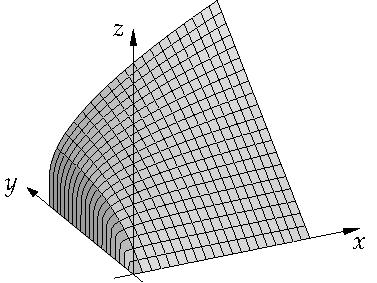
\includegraphics{figures/diffunderexample}
\caption{The graph $z= \frac{x^y-1}{\ln(x)}$ on $[0,1] \times [0,1]$.\label{fig:diffunderexample}}
\end{myfigureht}


Hence,
$g$ is a continuous function on $[0,1]$ and $g(0) = 0$.
For every $\epsilon > 0$, the $y$ derivative of the integrand, $x^y$,
is continuous on $[0,1] \times [\epsilon,1]$.  Therefore,
for $y >0$, we may differentiate under the integral sign,
\begin{equation*}
g'(y) =
\int_0^{1} \frac{\ln(x) x^y}{\ln(x)} \,dx 
=
\int_0^{1} x^y \,dx =
\frac{1}{y+1} .
\end{equation*}
We need to figure out $g(1)$ given that $g'(y) = \frac{1}{y+1}$ and $g(0) =
0$.  Elementary calculus says that $g(1) = \int_0^1 g'(y)\,dy = \ln(2)$.
Thus,
\begin{equation*}
\int_0^{1} \frac{x-1}{\ln(x)} \,dx  = \ln(2).
\end{equation*}
\end{example}

\subsection{Exercises}

\begin{exercise} \label{exercise:counterexamplediffunder}
Prove the two statements that were asserted in
\exampleref{example:counterexamplediffunder}:
\begin{enumerate}[a)]
\item
Prove $\frac{x-1}{\ln(x)}$ extends to a continuous function of
$[0,1]$.  That is, there exists a continuous function on $[0,1]$
that equals $\frac{x-1}{\ln(x)}$ on $(0,1)$.
\item
Prove $\frac{x^y-1}{\ln(x)}$ extends to a continuous function
on $[0,1] \times [0,1]$.
\end{enumerate}
\end{exercise}

\begin{exercise}
Suppose $h \colon \R \to \R$ is continuous and $g
\colon \R \to \R$ is continuously differentiable and compactly
supported.  That is, there exists some $M > 0$, such that $g(x) = 0$ whenever
$\abs{x} \geq M$.  Define
\begin{equation*}
f(x) \coloneqq \int_{-\infty}^\infty h(y)g(x-y)\,dy  .
\end{equation*}
Show that $f$ is differentiable.
\end{exercise}

\begin{exercise}
Suppose $f \colon \R \to \R$ is infinitely differentiable (all derivatives exist)
such that $f(0) = 0$.  Then show that there exists an infinitely
differentiable function $g \colon \R \to \R$ such that $f(x) = x\,g(x)$.
Show also that
if $f'(0) \not= 0$, then $g(0) \not= 0$.\\
Hint: Write
$f(x) = \int_0^x f'(s) \,ds$ and then rewrite the integral to go
from $0$ to $1$.
\end{exercise}

\begin{exercise}
Compute $\int_0^1 e^{tx} \,dx$.  Derive the formula for
$\int_0^1 x^n e^{x} \,dx$ not using integration by parts, but
by differentiation underneath the integral.
\end{exercise}

\begin{exercise}
Let $U \subset \R^n$ be an open set and suppose
$f(x,y_1,y_2,\ldots,y_n)$ is a continuous
function defined on $[0,1] \times U \subset \R^{n+1}$.
Suppose
$\frac{\partial f}{\partial y_1},
\frac{\partial f}{\partial y_2},\ldots,
\frac{\partial f}{\partial y_n}$
exist and are continuous on $[0,1] \times U$.
Then prove that $F \colon U \to \R$ defined by
\begin{equation*}
F(y_1,y_2,\ldots,y_n) \coloneqq
\int_0^1
f(x,y_1,y_2,\ldots,y_n)
\, dx
\end{equation*}
is continuously differentiable.
\end{exercise}

\begin{myfigureht}
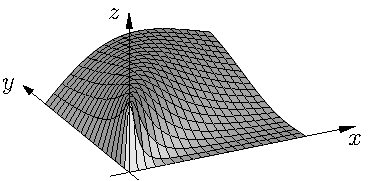
\includegraphics{figures/diffunderex916}
\caption{The graph $z= \frac{xy^3}{{(x^2+y^2)}^2}$ on
$[0,1] \times [0,1]$.\label{fig:diffunderex916}}
\end{myfigureht}

\begin{exercise}
\pagebreak[2]
Work out the following counterexample:  Let
\begin{equation*}
f(x,y) \coloneqq
\begin{cases}
\frac{xy^3}{{(x^2+y^2)}^2} & \text{if } x\not=0 \text{ or } y\not= 0, \\
0                          & \text{if } x=0 \text{ and } y=0.
\end{cases}
\end{equation*}
See \figureref{fig:diffunderex916}.
\begin{enumerate}[a)]
\item
Prove that for every fixed $y$, the function $x \mapsto f(x,y)$ is
Riemann integrable on $[0,1]$, and
\begin{equation*}
g(y) \coloneqq \int_0^1 f(x,y) \, dx = \frac{y}{2y^2+2} .
\end{equation*}
Therefore, $g'(y)$ exists and its derivative is the continuous function
\begin{equation*}
g'(y) =
\frac{d}{dy} \int_0^1 f(x,y) \, dx
=
\frac{1-y^2}{2{(y^2+1)}^2} .
\end{equation*}
\item
Prove $\frac{\partial f}{\partial y}$ exists at all $x$ and $y$ and
compute it.
\item
Show that for all $y$
\begin{equation*}
\int_0^1 \frac{\partial f}{\partial y} (x,y) \, dx
\end{equation*}
exists, but
\begin{equation*}
g'(0) \not= \int_0^1 \frac{\partial f}{\partial y} (x,0) \, dx .
\end{equation*}
\end{enumerate}
\end{exercise}

\begin{exercise}
\pagebreak[2]
Work out the following counterexample:  Let
\begin{equation*}
f(x,y) \coloneqq
\begin{cases}
x \,\sin \left(\frac{y}{x^2+y^2}\right) & \text{if } (x,y) \not= (0,0),\\
0                                       & \text{if } (x,y)=(0,0).
\end{cases}
\end{equation*}
\begin{enumerate}[a)]
\item
Prove $f$ is continuous on all of $\R^2$.
Therefore the following function is well-defined for every $y \in \R$:
\begin{equation*}
g(y) \coloneqq \int_0^1 f(x,y) \, dx .
\end{equation*}
\item
Prove $\frac{\partial f}{\partial y}$ exists for all $(x,y)$,
but is not continuous at $(0,0)$.
\item
Show that $\int_0^1 \frac{\partial f}{\partial y}(x,0) \, dx$ does not
exist even if we take improper integrals, that is,
that the limit
$\lim\limits_{h \to 0^+} \int_h^1 \frac{\partial f}{\partial y}(x,0) \, dx$
does not exist.
\end{enumerate}
Note: Feel free to use what you know about sine and cosine from calculus.
\end{exercise}

\begin{exercise} \label{exercise:strongerleibniz}
\pagebreak[3]
Strengthen the Leibniz integral rule in the following way.
Suppose $f \colon (a,b) \times (c,d) \to \R$ is a bounded continuous function,
such that $\frac{\partial f}{\partial y}$ exists for all $(x,y) \in (a,b)
\times (c,d)$ and is continuous and bounded.  Define
\begin{equation*}
g(y) \coloneqq \int_a^b f(x,y) \,dx .
\end{equation*}
Then $g \colon (c,d) \to \R$ is continuously differentiable and
\begin{equation*}
g'(y) = \int_a^b \frac{\partial f}{\partial y}(x,y) \,dx .
\end{equation*}
Hint: See also \volIref{\exerciseref*{vI-exercise:integralcontcontextra} and
\thmref*{vI-thm:dersconverge} from
volume I}{\exerciseref{exercise:integralcontcontextra} and
\thmref{thm:dersconverge}}.
\end{exercise}

%%%%%%%%%%%%%%%%%%%%%%%%%%%%%%%%%%%%%%%%%%%%%%%%%%%%%%%%%%%%%%%%%%%%%%%%%%%%%%

\sectionnewpage
\section{Path integrals}
\label{sec:pathintegral}

\sectionnotes{2--3 lectures}

\subsection{Piecewise smooth paths}

Let $\gamma \colon [a,b] \to \R^n$ be a function and write
$\gamma = (\gamma_1,\gamma_2,\ldots,\gamma_n)$. 
Suppose $\gamma$ is 
\emph{continuously differentiable},
that is,
it is differentiable and the derivative is continuous.
In other words, there exists a continuous function $\gamma^{\:\prime} \colon [a,b]
\to \R^n$ such that for every $t \in [a,b]$, we have
$\lim\limits_{h \to 0}
\frac{\snorm{\gamma(t+h)-\gamma(t) - \gamma^{\:\prime}(t) \, h}}{\sabs{h}} = 0$.
We treat
$\gamma^{\:\prime}(t)$ either as a linear operator (an $n \times 1$ matrix) or
a vector,
$\gamma^{\:\prime}(t) =
\bigl( \gamma_1^{\:\prime}(t), \gamma_2^{\:\prime}(t), \ldots,
\gamma_n^{\:\prime}(t) \bigr)$.
Equivalently, 
$\gamma_j$ is a continuously differentiable function on $[a,b]$
for every $j=1,2,\ldots,n$.
By \exerciseref{exercise:normonedim}, the operator norm of
the operator $\gamma^{\:\prime}(t)$ is equal to
the euclidean norm of the corresponding vector, so there is no
confusion when writing $\snorm{\gamma^{\:\prime}(t)}$.

\begin{defn}
A continuously differentiable function $\gamma \colon [a,b] \to \R^n$ is
called a \emph{\myindex{smooth path}}
or a
\emph{\myindex{continuously differentiable path}}\footnote{The
word \myquote{smooth} can sometimes mean
\myquote{infinitely differentiable} in the literature.}
if
$\gamma$ is continuously differentiable and
$\gamma^{\:\prime}(t) \not= 0$ for all $t \in [a,b]$.

The function $\gamma \colon [a,b] \to \R^n$ is called a
\emph{\myindex{piecewise smooth path}} or a
\emph{\myindex{piecewise continuously differentiable path}}
if there exist finitely many points
$t_0 = a < t_1 < t_2 < \cdots < t_k = b$ such that
the restriction $\gamma|_{[t_{j-1},t_j]}$ is smooth path for every
$j=1,2,\ldots,k$.

A path $\gamma$ is 
a \emph{\myindex{closed path}} if $\gamma(a) = \gamma(b)$, that is
if the path starts and ends in the same point.
A path $\gamma$ is a \emph{\myindex{simple path}} if 
either 1) $\gamma$ is a one-to-one function, or 2)
$\gamma|_{[a,b)}$ is one-to-one and $\gamma(a)=\gamma(b)$ ($\gamma$ is a
simple closed path).
\end{defn}


\begin{example} \label{mv:example:unitsquarepath}
Let $\gamma \colon [0,4] \to \R^2$ be defined by
\begin{equation*}
\gamma(t) \coloneqq
\begin{cases}
(t,0)   & \text{if } t \in [0,1],\\
(1,t-1) & \text{if } t \in (1,2],\\
(3-t,1) & \text{if } t \in (2,3],\\
(0,4-t) & \text{if } t \in (3,4].
\end{cases}
\end{equation*}
\begin{myfigureht}
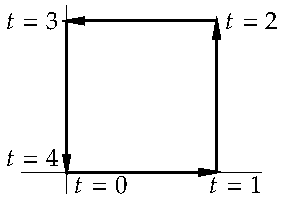
\includegraphics{figures/squarepath}
\caption{The path $\gamma$ traversing the unit square.\label{fig:squarepath}}
\end{myfigureht}

The path $\gamma$ is the unit square traversed
counterclockwise.  See \figureref{fig:squarepath}.  It is
a piecewise smooth path.  For example,
$\gamma|_{[1,2]}(t) = (1,t-1)$ and so
$(\gamma|_{[1,2]})'(t) = (0,1) \not= 0$.  Similarly for the other 3 sides.
Notice
that
$(\gamma|_{[1,2]})'(1) = (0,1)$,
$(\gamma|_{[0,1]})'(1) = (1,0)$, but
$\gamma^{\:\prime}(1)$ does not exist.  At the corners $\gamma$ is 
not differentiable.
The path $\gamma$ is a simple closed path, as $\gamma|_{[0,4)}$ is
one-to-one and $\gamma(0)=\gamma(4)$.
\end{example}

The definition of a piecewise smooth path as we have given it implies
continuity (exercise).  For general functions, many authors also
allow finitely many discontinuities, when they use the term \emph{piecewise
smooth}, and so one may say that we defined a piecewise smooth path
to be a \emph{\myindex{continuous piecewise smooth}} function.
While one may get by with smooth paths, for computations, the simplest
paths to write down are often piecewise smooth.

Generally, we are interested in the direct image $\gamma\bigl([a,b]\bigr)$,
rather than the specific parametrization, although that is also
important to some degree.  When we informally talk about a path or a curve,
we often mean the set $\gamma\bigl([a,b]\bigr)$, depending
on context.


\begin{example}
The condition $\gamma^{\:\prime}(t) \not= 0$ means that the image
$\gamma\bigl([a,b]\bigr)$
has no \myquote{corners} where $\gamma$ is smooth.
Consider 
\begin{equation*}
\gamma(t) \coloneqq
\begin{cases}
(t^2,0) & \text{if } t < 0,\\
(0,t^2) & \text{if } t \geq 0.
\end{cases}
\end{equation*}
See \figureref{fig:cornersmoothpath}.
It is left for the reader to check that $\gamma$ is continuously
differentiable, yet the image $\gamma(\R) = \bigl\{ (x,y) \in \R^2 : (x,y) =
(s,0) \text{ or } (x,y) = (0,s) \text{ for some } s \geq 0 \bigr\}$ has a
\myquote{corner} at the origin.  And that is because $\gamma^{\:\prime}(0) = (0,0)$.
More complicated examples with, say, infinitely many corners exist,
see the exercises.
\begin{myfigureht}
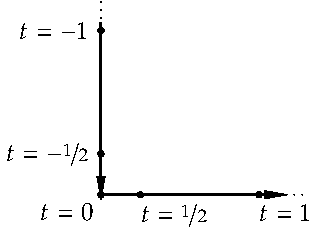
\includegraphics{figures/cornersmoothpath}
\caption{Smooth path with zero derivative with a corner.  Several values of
$t$ are marked with dots.\label{fig:cornersmoothpath}}
\end{myfigureht}
\end{example}

The condition $\gamma^{\:\prime}(t) \not= 0$ even at the endpoints guarantees
not only no corners, but also that the path ends nicely, that is, it can
extend a little bit past the endpoints.  Again, see the exercises.

\begin{example}
A graph of a continuously differentiable function $f \colon [a,b] \to \R$ is a smooth path.
Define $\gamma \colon [a,b] \to \R^2$ by
\begin{equation*}
\gamma(t) \coloneqq \bigl(t,f(t)\bigr) .
\end{equation*}
Then $\gamma^{\:\prime}(t) = \bigl( 1 , f'(t) \bigr)$, which is never zero,
and $\gamma\bigl([a,b]\bigr)$ is the graph of $f$.

There are other ways of parametrizing the path.  That is, there are
different paths with the same image.
The function $t \mapsto (1-t)a+tb$, takes the interval $[0,1]$ to $[a,b]$.
Define
$\alpha \colon [0,1] \to \R^2$ by
\begin{equation*}
\alpha(t) \coloneqq \bigl((1-t)a+tb,f((1-t)a+tb)\bigr) .
\end{equation*}
Then
$\alpha'(t) = \bigl( b-a ,~ (b-a)f'((1-t)a+tb) \bigr)$, which is never zero.
As sets, $\alpha\bigl([0,1]\bigr) = \gamma\bigl([a,b]\bigr)
= \bigl\{ (x,y) \in \R^2 : x \in [a,b] \text{ and } f(x) = y \bigr\}$,
which is just the graph of $f$.
\end{example}

The last example leads us to a definition.

\begin{defn}
Let $\gamma \colon [a,b] \to \R^n$ be a smooth path and
$h \colon [c,d] \to [a,b]$ a continuously differentiable bijective function
such that $h'(t) \not= 0$ for all $t \in [c,d]$.  Then
the composition
$\gamma \circ h$ is called a
\emph{\myindex{smooth reparametrization}}\index{reparametrization}
of $\gamma$.

Let $\gamma$ be a piecewise smooth path, and
$h$ a piecewise smooth bijective function with
nonzero one-sided limits of $h'$.
The composition
$\gamma \circ h$ is called a
\emph{\myindex{piecewise smooth reparametrization}} of $\gamma$.

If $h$ is strictly increasing, then $h$ is 
said to \emph{\myindex{preserve orientation}}.  If $h$ does not preserve
orientation, then $h$ is said to \emph{\myindex{reverse orientation}}.
\end{defn}

A reparametrization is another path for the same set.  That is,
$(\gamma \circ h)\bigl([c,d]\bigr) =
\gamma \bigl([a,b]\bigr)$.

The conditions on the piecewise smooth $h$ mean that
there is some partition $t_0 = c < t_1 < t_2 < \cdots < t_k = d$,
such that $h|_{[t_{j-1},t_j]}$ is continuously differentiable
and $(h|_{[t_{j-1},t_j]})'(t) \not= 0$ for all $t \in [t_{j-1},t_j]$.
Since $h$ is bijective, it is either strictly increasing or
strictly decreasing.  So either $(h|_{[t_{j-1},t_j]})'(t) > 0$
for all $t$ or $(h|_{[t_{j-1},t_j]})'(t) < 0$ for all $t$.

\begin{prop} \label{prop:reparamapiecewisesmooth}
If $\gamma \colon [a,b] \to \R^n$ is a piecewise smooth path,
and $\gamma \circ h \colon [c,d] \to \R^n$ is
a piecewise smooth reparametrization, then $\gamma \circ h$
is a piecewise smooth path.
\end{prop}

\begin{proof}
Assume that $h$ preserves orientation, that is, $h$ is strictly
increasing.
If $h \colon [c,d] \to [a,b]$ gives a piecewise smooth reparametrization,
then for some partition
$r_0 = c < r_1 < r_2 < \cdots < r_\ell = d$, the restriction
$h|_{[r_{j-1},r_j]}$ is continuously differentiable with a positive
derivative.

Let $t_0 = a < t_1 < t_2 < \cdots < t_k = b$ be the partition from the
definition of piecewise smooth for $\gamma$ together with the 
points $\{ h(r_0), h(r_1), h(r_2), \ldots, h(r_\ell) \}$.
Let $s_j \coloneqq h^{-1}(t_j)$.  Then
$s_0 = c < s_1 < s_2 < \cdots < s_k = d$
is a partition that includes (is a refinement of) the
$\{ r_0,r_1,\ldots,r_\ell \}$.
If $\tau \in [s_{j-1},s_j]$, then $h(\tau) \in [t_{j-1},t_j]$
since $h(s_{j-1}) = t_{j-1}$,
$h(s_{j}) = t_j$, and
$h$ is strictly increasing.
Also $h|_{[s_{j-1},s_j]}$ is continuously differentiable, and
$\gamma|_{[t_{j-1},t_j]}$ is also continuously differentiable.
Then
\begin{equation*}
(\gamma \circ h)|_{[s_{j-1},s_{j}]} (\tau)
=
\gamma|_{[t_{j-1},t_{j}]} \bigl( h|_{[s_{j-1},s_j]}(\tau) \bigr) .
\end{equation*}
The function 
$(\gamma \circ h)|_{[s_{j-1},s_{j}]}$ is therefore continuously
differentiable and
by the chain rule
\begin{equation*}
\bigl( (\gamma \circ h)|_{[s_{j-1},s_{j}]} \bigr) ' (\tau)
=
\bigl( \gamma|_{[t_{j-1},t_{j}]} \bigr)' \bigl( h(\tau) \bigr)
(h|_{[s_{j-1},s_j]})'(\tau) \not= 0 .
\end{equation*}
Consequently, $\gamma \circ h$ is a piecewise smooth path.
Orientation reversing $h$ is left as an exercise.
\end{proof}

If two paths are simple and their images are the same, it is
left as an exercise that there exists a reparametrization.
Here is where our assumption that $\gamma'$ is never zero is important.

\subsection{Path integral of a one-form}

\begin{defn}
Let $(x_1,x_2,\ldots,x_n) \in \R^n$ be our coordinates.
Given $n$ real-valued continuous functions
$\omega_1,\omega_2,\ldots,\omega_n$ defined on a set $S \subset \R^n$,
we define a \emph{\myindex{one-form}}\index{differential one-form}
to be an object of the form
\glsadd{not:oneform}
\begin{equation*}
\omega = \omega_1 \,dx_1 + \omega_2 \,dx_2 + \cdots + \omega_n \,dx_n .
\end{equation*}
We could represent $\omega$ as a continuous function from $S$ to $\R^n$,
although it is better to think of it as a different object.
\end{defn}

\begin{example}
\begin{equation*}
\omega(x,y) \coloneqq \frac{-y}{x^2+y^2} \,dx + \frac{x}{x^2+y^2} \,dy
\end{equation*}
is a one-form defined on $\R^2 \setminus \{ (0,0) \}$.
\end{example}

\begin{defn}
Let $\gamma \colon [a,b] \to \R^n$ be a smooth path
and let
\begin{equation*}
\omega = \omega_1 \,dx_1 + \omega_2 \,dx_2 + \cdots + \omega_n \,dx_n ,
\end{equation*}
be a one-form defined on the direct image $\gamma\bigl([a,b]\bigr)$.
Write $\gamma = (\gamma_1,\gamma_2,\ldots,\gamma_n)$.
Define:
\begin{equation*}
\begin{split}
\int_{\gamma} \omega
& \coloneqq
\int_a^b 
\Bigl(
\omega_1\bigl(\gamma(t)\bigr) \gamma_1^{\:\prime}(t) +
\omega_2\bigl(\gamma(t)\bigr) \gamma_2^{\:\prime}(t) + \cdots +
\omega_n\bigl(\gamma(t)\bigr) \gamma_n^{\:\prime}(t) \Bigr) dt
\\
&\phantom{:}=
\int_a^b 
\left(
\sum_{j=1}^n
\omega_j\bigl(\gamma(t)\bigr) \gamma_j^{\:\prime}(t) \right) dt .
\end{split}
\end{equation*}
To remember the definition note that $x_j$ is $\gamma_j(t)$, so
$dx_j$ becomes  $\gamma_j^{\:\prime}(t) \, dt$.

If $\gamma$ is piecewise smooth, take the corresponding partition
$t_0 = a < t_1 < t_2 < \ldots < t_k = b$, and assume the partition is
minimal
%\footnote{This restriction is not strictly necessary, but it 
%makes the integral immediately well-defined.}
in the sense that $\gamma$ is not differentiable
at $t_1,t_2,\ldots,t_{k-1}$.  As each $\gamma|_{[t_{j-1},t_j]}$ is
a smooth path, define
\begin{equation*}
\int_{\gamma} \omega
\coloneqq
\int_{\gamma|_{[t_0,t_1]}} \omega
\,
+
\,
\int_{\gamma|_{[t_1,t_2]}} \omega
\,
+ \, \cdots \, + \,
\int_{\gamma|_{[t_{k-1},t_k]}} \omega .
\end{equation*}
\end{defn}

The notation makes sense from the formula you remember from calculus,
let us state it somewhat informally:
If $x_j(t) = \gamma_j(t)$, then $dx_j = \gamma_j^{\:\prime}(t) \, dt$.

Paths can be cut up or concatenated.  The proof is a direct application
of the additivity of the Riemann integral, and is left as an exercise.
The proposition justifies why we defined the integral over a piecewise
smooth path in the way we did, and it justifies that we may as well
have taken any partition not just the minimal one in the definition.

\begin{prop} \label{mv:prop:pathconcat}
Let $\gamma \colon [a,c] \to \R^n$ be a piecewise smooth path,
and $b \in (a,c)$.
Define the piecewise smooth paths
$\alpha \coloneqq \gamma|_{[a,b]}$ and
$\beta \coloneqq \gamma|_{[b,c]}$.
Let $\omega$ be a one-form defined on
$\gamma\bigl([a,c]\bigr)$.  Then
\begin{equation*}
\int_{\gamma} \omega =
\int_{\alpha} \omega +
\int_{\beta} \omega .
\end{equation*}
\end{prop}


\begin{example} \label{example:mv:irrotoneformint}
Let the one-form $\omega$ and the path $\gamma \colon [0,2\pi] \to \R^2$ be defined by
\begin{equation*}
\omega(x,y) \coloneqq \frac{-y}{x^2+y^2} \,dx + \frac{x}{x^2+y^2} \,dy,
\qquad
\gamma(t) \coloneqq \bigl(\cos(t),\sin(t)\bigr) .
\end{equation*}
Then
\begin{equation*}
\begin{split}
\int_{\gamma} \omega
& =
\int_0^{2\pi}
\Biggl(
\frac{-\sin(t)}{{\bigl(\cos(t)\bigr)}^2+{\bigl(\sin(t)\bigr)}^2}
\bigl(-\sin(t)\bigr)
+
\frac{\cos(t)}{{\bigl(\cos(t)\bigr)}^2+{\bigl(\sin(t)\bigr)}^2}
\bigl(\cos(t)\bigr)
\Biggr) \, dt
\\
& =
\int_0^{2\pi}
1 \, dt
= 2\pi .
\end{split}
\end{equation*}
Next, let us parametrize the same curve as
$\alpha \colon [0,1] \to \R^2$ defined by $\alpha(t) \coloneqq \bigl(\cos(2\pi
t),\sin(2 \pi t)\bigr)$, that is $\alpha$ is a smooth reparametrization of
$\gamma$.  Then
\begin{equation*}
\begin{split}
\int_{\alpha} \omega
& =
\int_0^{1}
\Biggl(
\frac{-\sin(2\pi t)}{{\bigl(\cos(2\pi t)\bigr)}^2+{\bigl(\sin(2\pi t)\bigr)}^2}
\bigl(-2\pi \sin(2\pi t)\bigr)
\\
& \phantom{=\int_0^1\Biggl(~}
+
\frac{\cos(2 \pi t)}{{\bigl(\cos(2 \pi t)\bigr)}^2+{\bigl(\sin(2 \pi t)\bigr)}^2}
\bigl(2 \pi \cos(2 \pi t)\bigr)
\Biggr) \, dt
\\
& =
\int_0^{1}
2\pi \, dt
= 2\pi .
\end{split}
\end{equation*}
Now let us reparametrize with $\beta \colon [0,2\pi] \to \R^2$
as $\beta(t) \coloneqq \bigl(\cos(-t),\sin(-t)\bigr)$.  Then
\begin{equation*}
\begin{split}
\int_{\beta} \omega
& =
\int_0^{2\pi}
\Biggl(
\frac{-\sin(-t)}{{\bigl(\cos(-t)\bigr)}^2+{\bigl(\sin(-t)\bigr)}^2}
\bigl(\sin(-t)\bigr)
+
\frac{\cos(-t)}{{\bigl(\cos(-t)\bigr)}^2+{\bigl(\sin(-t)\bigr)}^2}
\bigl(-\cos(-t)\bigr)
\Biggr) \, dt
\\
& =
\int_0^{2\pi}
(-1) \, dt
= -2\pi .
\end{split}
\end{equation*}
The path $\alpha$ is an orientation preserving reparametrization of
$\gamma$, and the integrals are the same.  The path $\beta$
is an orientation reversing reparametrization of $\gamma$ and the integral is
minus the original.  See \figureref{fig:circlepathrepar}.
\begin{myfigureht}
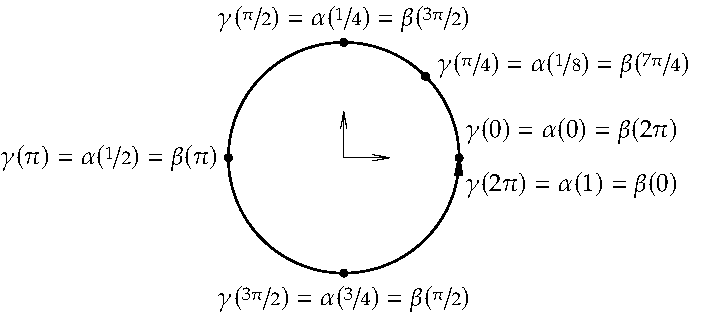
\includegraphics{figures/circlepathrepar}
\caption{A circular path reparametrized in two different ways. The arrow
indicates the orientation of $\gamma$ and $\alpha$. The path $\beta$ traverses
the circle in the
opposite direction.\label{fig:circlepathrepar}}
\end{myfigureht}
\end{example}

The previous example is not a fluke.
The path integral does not depend on the parametrization of
the curve, the only thing that matters is the direction in which the curve
is traversed.

\begin{prop} \label{mv:prop:pathintrepararam}
Let $\gamma \colon [a,b] \to \R^n$ be a piecewise smooth path and
$\gamma \circ h \colon [c,d] \to \R^n$ a piecewise smooth reparametrization.
Suppose $\omega$ is a one-form defined on the set $\gamma\bigl([a,b]\bigr)$.  Then
\begin{equation*}
\int_{\gamma \circ h} \omega =
\begin{cases}
\int_{\gamma} \omega  & \text{if } h \text{ preserves orientation,}\\
-\int_{\gamma} \omega & \text{if } h \text{ reverses orientation.}
\end{cases}
\end{equation*}
\end{prop}

\begin{proof}
Assume first that $\gamma$ and $h$ are both smooth.
Write $\omega = \omega_1 \, dx_1 + \omega_2 \, dx_2 + \cdots +
\omega_n \, dx_n$.
Suppose that $h$ is orientation preserving.  Use
the change of variables formula for the Riemann integral:
\begin{equation*}
\begin{split}
\int_{\gamma} \omega
& =
\int_a^b 
\left(
\sum_{j=1}^n
\omega_j\bigl(\gamma(t)\bigr) \gamma_j^{\:\prime}(t)
\right) dt
\\
& =
\int_c^d 
\left(
\sum_{j=1}^n
\omega_j\Bigl(\gamma\bigl(h(\tau)\bigr)\Bigr) \gamma_j^{\:\prime}\bigl(h(\tau)\bigr)
\right) h'(\tau) \, d\tau
\\
& =
\int_c^d 
\left(
\sum_{j=1}^n
\omega_j\Bigl(\gamma\bigl(h(\tau)\bigr)\Bigr) (\gamma_j \circ h)'(\tau)
\right) d\tau
=
\int_{\gamma \circ h} \omega .
\end{split}
\end{equation*}
If $h$ is orientation reversing, it swaps the order of the limits on the
integral and introduces a minus sign.
The details, along with finishing the proof for piecewise smooth
paths, is left as \exerciseref{mv:exercise:pathpiece}.
\end{proof}

Due to this proposition (and the exercises), if $\Gamma
\subset \R^n$ is the image of a simple piecewise smooth path
$\gamma\bigl([a,b]\bigr)$, then as long as we somehow indicate the orientation, that
is, the direction in which we traverse the curve, we can write
\begin{equation*}
\int_{\Gamma} \omega ,
\end{equation*}
without mentioning the specific $\gamma$.
Furthermore, for a simple closed path, it does not even matter where we
start the parametrization.  See the exercises.

Recall that \emph{simple} means that $\gamma$
is one-to-one except perhaps at the endpoints, in particular
it is one-to-one when restricted to $[a,b)$.
We may relax the condition that the path is simple a little bit.
For example, it is enough to suppose that
$\gamma \colon [a,b] \to \R^n$ is one-to-one except at finitely many points.
%That is, there is a finite set $S \subset [a,b]$
%and $\gamma|_{[a,b]\setminus S}$ is one-to-one.
See \exerciseref{mv:exercise:curveintegral}.  But we cannot remove
the condition completely as is
illustrated by the following example.

\begin{example}
Suppose $\gamma \colon [0,2\pi] \to \R^2$ is given by $\gamma(t) \coloneqq
\bigl(\cos(t),\sin(t)\bigr)$, and
$\beta \colon [0,2\pi] \to \R^2$ by $\beta(t) \coloneqq
\bigl(\cos(2t),\sin(2t)\bigr)$.  Notice that
$\gamma\bigl([0,2\pi]\bigr) = \beta\bigl([0,2\pi]\bigr)$; we travel
around the same curve, the unit circle.  But $\gamma$ goes around the unit
circle once in the counter clockwise direction, and $\beta$ goes around the
unit circle twice (in the same direction). 
See \figureref{fig:circlepathrepar2}.
\begin{myfigureht}
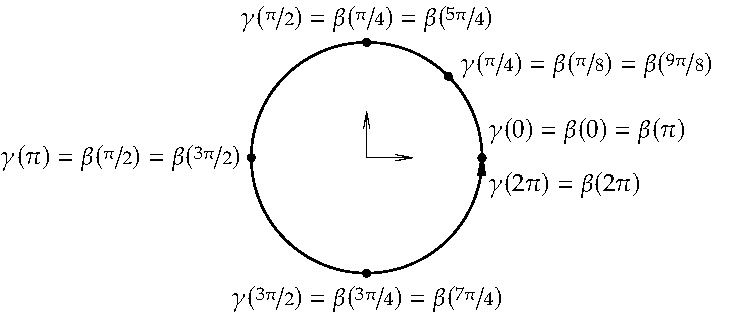
\includegraphics{figures/circlepathrepar2}
\caption{Circular path traversed once by
$\gamma \colon [0,2\pi] \to \R^2$
and twice by
$\beta \colon [0,2\pi] \to \R^2$.\label{fig:circlepathrepar2}}
\end{myfigureht}

Compute
\begin{align*}
& \int_{\gamma} -y\, dx + x\,dy
=
\int_0^{2\pi}
\Bigl( \bigl(-\sin(t) \bigr) \bigl(-\sin(t) \bigr) + \cos(t) \cos(t) \Bigr) dt
=
2 \pi,\\
& \int_{\beta} -y\, dx + x\,dy
=
\int_0^{2\pi}
\Bigl( \bigl(-\sin(2t) \bigr) \bigl(-2\sin(2t) \bigr) + \cos(t)
\bigl(2\cos(t)\bigr) \Bigr) dt
=
4 \pi.
\end{align*}
\end{example}

It is sometimes convenient to define a path integral over $\gamma \colon
[a,b] \to \R^n$ that is not a path.
Define
\glsadd{not:pathintegralomega}
\begin{equation*}
\int_{\gamma} \omega \coloneqq \int_a^b
\left(
\sum_{j=1}^n
\omega_j\bigl(\gamma(t)\bigr) \gamma_j^{\:\prime}(t)
\right) dt 
\end{equation*}
for every continuously differentiable $\gamma$.  A 
case that comes up naturally is when $\gamma$ is constant.  Then
$\gamma^{\:\prime}(t) = 0$ for all $t$, and $\gamma\bigl([a,b]\bigr)$ is a single
point, which we regard as a \myquote{curve} of length zero.  Then,
$\int_{\gamma} \omega = 0$ for every $\omega$.

\subsection{Path integral of a function}

Next, we integrate a function against the so-called
\emph{\myindex{arc-length measure}} $ds$.  The geometric picture we have in mind
is the area under the graph of the function over a path.
Imagine a fence erected over $\gamma$ with height given by the function
and the integral is the area of the fence.
See \figureref{fig:fenceintegral}.
\begin{myfigureht}
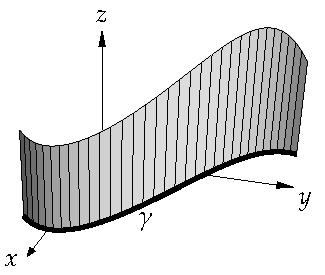
\includegraphics{figures/fenceintegral}
\caption{A path $\gamma \colon [a,b] \to \R^2$ in the $xy$-plane (bold curve), and a function
$z=f(x,y)$ graphed above it in the $z$ direction.  The integral is the
shaded area depicted.\label{fig:fenceintegral}}
\end{myfigureht}

\begin{defn}
Suppose $\gamma \colon [a,b] \to \R^n$ is a smooth path, and $f$ is a
continuous function defined on the image $\gamma\bigl([a,b]\bigr)$.  Then
define
\glsadd{not:lineintegralf}
\begin{equation*}
\int_{\gamma} f \,ds \coloneqq
\int_a^b f\bigl( \gamma(t) \bigr) \snorm{\gamma^{\:\prime}(t)} \, dt .
\end{equation*}
To emphasize the variables we may use
\begin{equation*}
\int_{\gamma} f(x) \,ds(x) \coloneqq \int_{\gamma} f \,ds .
\end{equation*}

The definition for a piecewise smooth path is similar as before and is left
to the reader.
\end{defn}

The path integral of a function is also independent of the parametrization,
and in this case, the orientation does not matter.

\begin{prop} \label{mv:prop:lineintrepararam}
Let $\gamma \colon [a,b] \to \R^n$ be a piecewise smooth path and
$\gamma \circ h \colon [c,d] \to \R^n$ a piecewise smooth reparametrization.
Suppose $f$ is a continuous function defined on the set
$\gamma\bigl([a,b]\bigr)$.  Then
\begin{equation*}
\int_{\gamma \circ h} f\, ds = \int_{\gamma} f\, ds .
\end{equation*}
\end{prop}

\begin{proof}
Suppose $h$ is orientation preserving and that $\gamma$ and $h$
are both smooth.  Then 
\begin{equation*}
\begin{split}
\int_{\gamma} f \, ds
& =
\int_a^b 
f\bigl(\gamma(t)\bigr) \snorm{\gamma^{\:\prime}(t)} \, dt
\\
& =
\int_c^d 
f\Bigl(\gamma\bigl(h(\tau)\bigr)\Bigr)
\snorm{\gamma^{\:\prime}\bigl(h(\tau)\bigr)} h'(\tau) \, d\tau
\\
& =
\int_c^d 
f\Bigl(\gamma\bigl(h(\tau)\bigr)\Bigr)
\snorm{\gamma^{\:\prime}\bigl(h(\tau)\bigr) h'(\tau)} \, d\tau
\\
& =
\int_c^d 
f\bigl((\gamma \circ h)(\tau)\bigr) \snorm{(\gamma \circ h)'(\tau)} \, d\tau
\\
& = 
\int_{\gamma \circ h} f \, ds .
\end{split}
\end{equation*}
If $h$ is orientation reversing it swaps the order of the limits on the
integral, but you also have to introduce a minus sign in order
to take $h'$ inside the norm.
The details, along with finishing the proof for piecewise smooth
paths is left to the reader as \exerciseref{mv:exercise:linepiece}.
\end{proof}

As before,
due to this proposition (and the exercises),
if $\gamma$ is simple, it does not matter which
parametrization we use.  Therefore, if $\Gamma = \gamma\bigl( [a,b] \bigr)$, we can
simply write
\begin{equation*}
\int_\Gamma f\, ds .
\end{equation*}
In this case we do not need to worry about orientation, either way we
get the same integral.

\begin{example}
Let $f(x,y) \coloneqq x$.  Let $C \subset \R^2$ be half of the unit circle for $x
\geq 0$.  We wish to compute
\begin{equation*}
\int_C f \, ds .
\end{equation*}
Parametrize the curve $C$ via $\gamma \colon
[\nicefrac{-\pi}{2},\nicefrac{\pi}{2}] \to \R^2$ defined as
$\gamma(t) \coloneqq \bigl(\cos(t),\sin(t)\bigr)$.
Then $\gamma^{\:\prime}(t) = \bigl(-\sin(t),\cos(t)\bigr)$, and
\begin{equation*}
\int_C f \, ds =
\int_\gamma f \, ds
=
\int_{-\pi/2}^{\pi/2} \cos(t) \sqrt{ {\bigl(-\sin(t)\bigr)}^2 +  
{\bigl(\cos(t)\bigr)}^2 } \, dt
=
\int_{-\pi/2}^{\pi/2} \cos(t) \, dt = 2.
\end{equation*}
\end{example}

\begin{defn}
Suppose $\Gamma \subset \R^n$ is parametrized by a simple
piecewise smooth path $\gamma \colon [a,b] \to \R^n$, that is
$\gamma\bigl( [a,b] \bigr) = \Gamma$.  We define the
\emph{\myindex{length}}\index{length of a curve} by
\begin{equation*}
\ell(\Gamma) \coloneqq \int_{\Gamma} ds = \int_{\gamma} ds .
\end{equation*}
\end{defn}

If $\gamma$ is smooth,
\begin{equation*}
\ell(\Gamma) = 
\int_a^b
\snorm{\gamma^{\:\prime}(t)}\, dt .
\end{equation*}
This may be a good time to mention that it is common to write
$\int_a^b
\snorm{\gamma^{\:\prime}(t)}\, dt$ even if the path is only piecewise smooth.
That is because $\snorm{\gamma^{\:\prime}(t)}$ is defined and continuous
at all but finitely many points and is bounded, and so the integral exists.

\begin{example}
Let $x,y \in \R^n$ be two points and write $[x,y]$ as the straight line
segment between the two points $x$ and $y$.  Parametrize
$[x,y]$ by $\gamma(t) \coloneqq (1-t)x + ty$ for $t$ running between $0$ and $1$.
See \figureref{fig:straightpath}.
Then $\gamma^{\:\prime}(t) = y-x$, and therefore
\begin{equation*}
\ell\bigl([x,y]\bigr)
=
\int_{[x,y]} ds
=
\int_0^1 \snorm{y-x} \, dt
=
\snorm{y-x} .
\end{equation*}
The length of $[x,y]$ is the standard euclidean distance between $x$ and $y$,
justifying the name.
\begin{myfigureht}
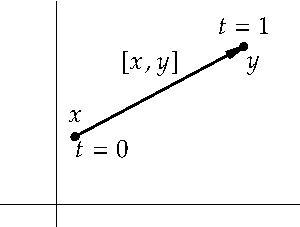
\includegraphics{figures/straightpath}
\caption{Straight path between $x$ and $y$ parametrized
by $(1-t)x + ty$.\label{fig:straightpath}}
\end{myfigureht}
\end{example}

A simple piecewise smooth path $\gamma \colon [0,r] \to \R^n$ is
said to be an \emph{\myindex{arc-length parametrization}} if
for all $t \in [0,r]$, we have
\begin{equation*}
\ell\bigl( \gamma\bigl([0,t]\bigr) \bigr) = t .
\end{equation*}
If $\gamma$ is smooth, then
\begin{equation*}
\int_0^t d\tau =
t = \ell\bigl( \gamma\bigl([0,t]\bigr) \bigr) =
\int_0^t
\snorm{\gamma^{\:\prime}(\tau)}
\, d\tau
\end{equation*}
for all $t$,
which means that $\snorm{\gamma^{\:\prime}(t)} = 1$ for all $t$.
Similarly for piecewise smooth $\gamma$, we get
$\snorm{\gamma^{\:\prime}(t)} = 1$ for all $t$ where the derivative exists.
So you can think of such a parametrization as moving around your curve at speed
1.  If $\gamma \colon [0,r] \to \R^n$ is an arclength parametrization, it is
common to use $s$ as the variable as $\int_\gamma f \,ds
= \int_0^r f\bigl(\gamma(s)\bigr) \,ds$.

\subsection{Exercises}

\begin{exercise}
Show that if $\varphi \colon [a,b] \to \R^n$ is a piecewise smooth path as we
defined it, then $\varphi$ is a continuous function.
\end{exercise}

\begin{exercise}
Finish the proof of \propref{prop:reparamapiecewisesmooth} for orientation
reversing reparametrizations.
\end{exercise}

\begin{exercise}
Prove \propref{mv:prop:pathconcat}.
\end{exercise}

\begin{exercise} \label{mv:exercise:pathpiece}
Finish the proof of \propref{mv:prop:pathintrepararam}
for
\begin{enumerate}[a)]
\item
orientation reversing reparametrizations, and
\item
piecewise smooth paths
and reparametrizations.
\end{enumerate}
\end{exercise}

\begin{exercise} \label{mv:exercise:linepiece}
Finish the proof of \propref{mv:prop:lineintrepararam}
for
\begin{enumerate}[a)]
\item
orientation reversing reparametrizations, and
\item
piecewise smooth paths
and reparametrizations.
\end{enumerate}
\end{exercise}

\begin{exercise}
Suppose $\gamma \colon [a,b] \to \R^n$ is a piecewise smooth path, and $f$ is a
continuous function defined on the image $\gamma\bigl([a,b]\bigr)$.
Provide a definition of $\int_{\gamma} f \,ds$.
\end{exercise}

\begin{exercise}
Directly using the definitions compute:
\begin{enumerate}[a)]
\item
The arc-length of the unit square from
\exampleref{mv:example:unitsquarepath} using the given parametrization.
\item
The arc-length of the unit circle using the parametrization
$\gamma \colon [0,1] \to \R^2$, $\gamma(t) \coloneqq \bigl(\cos(2\pi t),\sin(2\pi t)\bigr)$.
\item
The arc-length of the unit circle using the parametrization
$\beta \colon [0,2\pi] \to \R^2$, $\beta(t) \coloneqq \bigl(\cos(t),\sin(t)\bigr)$.
\end{enumerate}
Note: Feel free to use what you know about sine and cosine from calculus.
\end{exercise}

\begin{exercise}
Suppose $\gamma \colon [0,1] \to \R^n$ is a smooth path, and
$\omega$ is a one-form defined on the image $\gamma\bigl([a,b]\bigr)$.
For $r \in [0,1]$, let $\gamma_r \colon [0,r] \to \R^n$ be defined
as simply the restriction of $\gamma$ to $[0,r]$.  Show that the
function $h(r) \coloneqq \int_{\gamma_r} \omega$ is a continuously
differentiable function on $[0,1]$.
\end{exercise}

\begin{exercise}
Suppose $\gamma \colon [a,b] \to \R^n$ is a smooth path.
Show that there exists an $\epsilon > 0$ and a smooth function
$\widetilde{\gamma} \colon (a-\epsilon,b+\epsilon) \to \R^n$
with $\widetilde{\gamma}(t) = \gamma(t)$ for all $t \in [a,b]$
and $\widetilde{\gamma}^{\:\prime}(t) \not= 0$ for all $t \in 
(a-\epsilon,b+\epsilon)$.  That is, prove that a smooth path extends
some small distance past the end points.
\end{exercise}

\begin{exercise} 
Suppose $\alpha \colon [a,b] \to \R^n$ and
$\beta \colon [c,d] \to \R^n$ are piecewise smooth paths such that
$\Gamma \coloneqq \alpha\bigl([a,b]\bigr) = \beta\bigl([c,d]\bigr)$.
Show that there exist finitely many points
$\{ p_1,p_2,\ldots,p_k\} \in \Gamma$, such that
the sets
$\alpha^{-1}\bigl( \{ p_1,p_2,\ldots,p_k\} \bigr)$
and
$\beta^{-1}\bigl( \{ p_1,p_2,\ldots,p_k\} \bigr)$
are partitions of $[a,b]$ and $[c,d]$ such that on every subinterval
the paths are smooth (that is, they are partitions as in the definition
of piecewise smooth path).
\end{exercise}

\begin{exercise}
\pagebreak[3]
\leavevmode
\begin{enumerate}[a)]
\item
Suppose $\gamma \colon [a,b] \to \R^n$ and $\alpha \colon [c,d] \to \R^n$
are two smooth paths that are one-to-one and
$\gamma\bigl([a,b]\bigr) = \alpha\bigl([c,d]\bigr)$.  Then
there exists a smooth reparametrization $h \colon [a,b] \to [c,d]$
such that $\gamma = \alpha \circ h$.\\
Hint 1: It is not hard to show $h$ exists.
The trick is to prove it is continuously differentiable
with a nonzero derivative.  Apply the implicit function
theorem though it may at first seem the dimensions are wrong.\\
Hint 2: Worry about derivative of $h$ in $(a,b)$ first.
\item
Prove the same thing as part a, but now for simple closed paths with the
further assumption that $\gamma(a) = \gamma(b) = \alpha(c) = \alpha(d)$.
\item
Prove parts a) and b) but for piecewise smooth paths, obtaining
piecewise smooth reparametrizations.\\
Hint: The trick is to find two
partitions such that when restricted to a subinterval of the partition
both paths have the same image and are smooth, see the exercise above.
\end{enumerate}
\end{exercise}

\begin{exercise} 
\pagebreak[1]
Suppose $\alpha \colon [a,b] \to \R^n$ and
$\beta \colon [b,c] \to \R^n$ are piecewise smooth paths with
$\alpha(b)=\beta(b)$.  Let $\gamma \colon [a,c] \to \R^n$ be defined by
\begin{equation*}
\gamma(t) \coloneqq
\begin{cases}
\alpha(t) & \text{if } t \in [a,b], \\
\beta(t)  & \text{if } t \in (b,c].
\end{cases}
\end{equation*}
Show that $\gamma$ is a piecewise smooth path, and that if $\omega$ is a
one-form defined on the curve given by $\gamma$, then
\begin{equation*}
\int_{\gamma} \omega =
\int_{\alpha} \omega +
\int_{\beta} \omega .
\end{equation*}
\end{exercise}

\begin{exercise} \label{mv:exercise:closedcurveintegral}
\pagebreak[1]
Suppose $\gamma \colon [a,b] \to \R^n$ and
$\beta \colon [c,d] \to \R^n$ are two simple closed piecewise smooth paths.
That is, $\gamma(a)=\gamma(b)$ and $\beta(c) = \beta(d)$ and
the restrictions $\gamma|_{[a,b)}$ and $\beta|_{[c,d)}$ are one-to-one.
Suppose $\Gamma = \gamma\bigl([a,b]\bigr) = \beta\bigl([c,d]\bigr)$ and
$\omega$ is a one-form defined on $\Gamma \subset \R^n$.  Show that either
\begin{equation*}
\int_\gamma \omega = 
\int_\beta \omega,
\qquad \text{or} \qquad 
\int_\gamma \omega = 
- \int_\beta \omega.
\end{equation*}
In particular, the notation $\int_{\Gamma} \omega$ makes sense if we indicate
the direction in which the integral is evaluated.
Hint: See previous three exercises.
\end{exercise}

\begin{exercise} \label{mv:exercise:curveintegral}
Suppose $\gamma \colon [a,b] \to \R^n$ and
$\beta \colon [c,d] \to \R^n$ are two piecewise smooth paths
which are one-to-one except at finitely many points.  That is,
there exist finite sets $S \subset [a,b]$ and $T \subset [c,d]$
such that $\gamma|_{[a,b]\setminus S}$ and
$\beta|_{[c,d]\setminus T}$ are one-to-one.
Suppose $\Gamma = \gamma\bigl([a,b]\bigr) = \beta\bigl([c,d]\bigr)$ and $\omega$ is a
one-form defined on $\Gamma \subset \R^n$.  Show that either
\begin{equation*}
\int_\gamma \omega = 
\int_\beta \omega,
\qquad \text{or} \qquad 
\int_\gamma \omega = 
- \int_\beta \omega.
\end{equation*}
In particular, the notation $\int_{\Gamma} \omega$ makes sense if we indicate
the direction in which the integral is evaluated.
\\
Hint: Same hint as the last exercise.
\end{exercise}

\begin{exercise}
Define $\gamma \colon [0,1] \to \R^2$ by
$\gamma(t) \coloneqq \Bigl( t^3 \sin(\nicefrac{1}{t}),\,
t{\bigl(3t^2\sin(\nicefrac{1}{t})-t\cos(\nicefrac{1}{t})\bigr)}^2 \Bigr)$
for
$t \not= 0$ and $\gamma(0) = (0,0)$.  Show that
\begin{enumerate}[a)]
\item
$\gamma$ is continuously differentiable on $[0,1]$.
\item
Show that there exists an infinite sequence $\{ t_n \}_{n=1}^\infty$ in $[0,1]$
converging to 0, such that
$\gamma^{\:\prime}(t_n) = (0,0)$.
\item
Show that the points $\gamma(t_n)$ lie on the line $y=0$ and such
that the $x$-coordinate of $\gamma(t_n)$ alternates between positive and
negative (if they do not alternate you only found a subsequence,
you need to find them all).
\item
Show that there is no piecewise smooth $\alpha$ whose image equals
$\gamma\bigl([0,1]\bigr)$.  Hint: Look at part c) and show that $\alpha'$
must be zero where it reaches the origin.
\item
(Computer) If you know a plotting software that allows you to plot
parametric curves, make a plot of the curve, but only for $t$ in the
range $[0,0.1]$ otherwise you will not see the behavior.  In particular, you
should notice that $\gamma\bigl([0,1]\bigr)$ has infinitely many
\myquote{corners}
near the origin.
\end{enumerate}
Note: Feel free to use what you know about sine and cosine from calculus.
\end{exercise}

%%%%%%%%%%%%%%%%%%%%%%%%%%%%%%%%%%%%%%%%%%%%%%%%%%%%%%%%%%%%%%%%%%%%%%%%%%%%%%

\sectionnewpage
\section{Path independence}
\label{sec:pathind}

\sectionnotes{2 lectures}

\subsection{Path independent integrals}

Let $U \subset \R^n$ be a set and $\omega$ a one-form defined on $U$.
The integral of $\omega$
is said to be \emph{\myindex{path independent}}
if for every pair of points $x,y \in U$ and
every pair of piecewise smooth paths
$\gamma \colon [a,b] \to U$ and
$\beta \colon [c,d] \to U$ such that $\gamma(a) = \beta(c) = x$
and $\gamma(b) = \beta(d) = y$, we have
\begin{equation*}
\int_\gamma \omega = \int_\beta \omega .
\end{equation*}
In this case, we simply write
\begin{equation*}
\int_x^y \omega \coloneqq \int_\gamma \omega = \int_\beta \omega .
\end{equation*}
Not every one-form gives a path independent integral.  Most do not.

\begin{example}
Let $\gamma \colon [0,1] \to \R^2$ be the path $\gamma(t) \coloneqq (t,0)$
going from $(0,0)$ to $(1,0)$.  Let $\beta \colon [0,1] \to \R^2$ be the path
$\beta(t) \coloneqq \bigl(t,(1-t)t\bigr)$ also going between the same points.  Then
\begin{align*}
& \int_\gamma y \, dx = 
\int_0^1 \gamma_2(t) \gamma_1^{\:\prime}(t) \, dt
=
\int_0^1 0 (1) \, dt = 0 ,\\
& \int_\beta y \, dx = 
\int_0^1 \beta_2(t) \beta_1'(t) \, dt
=
\int_0^1 (1-t)t(1) \, dt = \frac{1}{6} .
\end{align*}
The integral of $y\,dx$ is not path independent.
In particular,
$\int_{(0,0)}^{(1,0)} y\,dx$ does not make sense.
\end{example}

\begin{defn}
Let $U \subset \R^n$ be an open set and $f \colon U \to \R$ a 
continuously differentiable function.  The one-form
\begin{equation*}
df \coloneqq
\frac{\partial f}{\partial x_1} \, dx_1 + 
\frac{\partial f}{\partial x_2} \, dx_2 + \cdots +
\frac{\partial f}{\partial x_n} \, dx_n 
\end{equation*}
is called the \emph{\myindex{total derivative}} of $f$.

An open set $U \subset \R^n$ is said to be \emph{\myindex{path connected}}%
\footnote{Normally only a continuous path is used in this definition, but
for open sets the two definitions are equivalent.  See the exercises.}
if for every two points $x$ and $y$ in $U$, there exists a piecewise smooth
path starting at $x$ and ending at $y$.
\end{defn}

We leave as an exercise that every connected open set is path
connected.

\begin{prop} \label{mv:prop:pathinddf}
Let $U \subset \R^n$ be a path connected open set and $\omega$ a one-form
defined on $U$.  Then
$\int_x^y \omega$
is path independent (for all $x,y \in U$) if and only if there exists
a continuously differentiable $f \colon U \to \R$ such that $\omega = df$.

In fact, if such an $f$ exists, then for every pair of points $x,y \in U$
\begin{equation*}
\int_{x}^y \omega = f(y)-f(x) .
\end{equation*}
\end{prop}

In other words, if we fix $p \in U$, then $f(x) = C + \int_{p}^x \omega$
for some constant $C$.

\begin{proof}
First suppose that the integral is path independent.  Pick $p \in U$.  Since
$U$ is path connected, there exists a path from $p$ to every $x \in U$.
Define
\begin{equation*}
f(x) \coloneqq \int_{p}^x \omega .
\end{equation*}
Write $\omega = \omega_1 \,dx_1 + \omega_2 \,dx_2 + \cdots + \omega_n \,dx_n$.
We wish to show that for every $j = 1,2,\ldots,n$, the
partial derivative $\frac{\partial f}{\partial x_j}$ exists
and is equal to $\omega_j$.

Let $e_j$ be an arbitrary standard basis vector, and $h$ a nonzero real
number.  Compute
\begin{equation*}
\frac{f(x+h e_j) - f(x)}{h} =
\frac{1}{h} \left( \int_{p}^{x+he_j} \omega - \int_{p}^x \omega \right)
=
\frac{1}{h} \int_{x}^{x+he_j} \omega ,
\end{equation*}
which follows by \propref{mv:prop:pathconcat} and path independence as 
$\int_{p}^{x+he_j} \omega =
\int_{p}^{x} \omega +
\int_{x}^{x+he_j} \omega$, because we pick a path from $p$ to
$x+he_j$ that also happens to pass through $x$, and then we cut this path in
two, see \figureref{fig:pathindantider}.

\begin{myfigureht}
\subimport*{figures/}{pathindantider.pdf_t}
\caption{Using path independence in computing the partial
derivative.\label{fig:pathindantider}}
\end{myfigureht}


Since $U$ is open, suppose $h$ is so small so that all points of distance
$\abs{h}$ or
less from $x$ are in $U$.
As the integral is path independent,
pick the simplest path possible from $x$ to $x+he_j$, that is
$\gamma(t) \coloneqq x+t he_j$ for $t \in [0,1]$.  The path is in $U$.
Notice $\gamma^{\:\prime}(t) = h e_j$
has only one nonzero component and that is the $j$th component, which is
$h$.  Therefore,
\begin{equation*}
\frac{1}{h} \int_{x}^{x+he_j} \omega 
=
\frac{1}{h} \int_{\gamma} \omega 
=
\frac{1}{h} \int_0^1 \omega_j(x+the_j) h \, dt 
=
\int_0^1 \omega_j(x+the_j) \, dt  .
\end{equation*}
We wish to take the limit as $h \to 0$.  The function $\omega_j$ is
continuous at $x$.  Given $\epsilon > 0$, suppose $h$ is small enough so that
$\abs{\omega_j(x)-\omega_j(y)} < \epsilon$ whenever $\snorm{x-y} \leq \abs{h}$.
Thus,
$\abs{\omega_j(x+the_j)-\omega_j(x)} < \epsilon$ for all $t \in [0,1]$,
and we estimate
\begin{equation*}
\abs{\int_0^1 \omega_j(x+the_j) \, dt  - \omega_j(x)}
=
\abs{\int_0^1 \bigl( \omega_j(x+the_j) - \omega_j(x) \bigr) \, dt}
\leq
\epsilon .
\end{equation*}
That is,
\begin{equation*}
\lim_{h\to 0}\frac{f(x+h e_j) - f(x)}{h} = \omega_j(x) .
\end{equation*}
All partials of $f$ exist and are equal to $\omega_j$, which are continuous
functions.  Thus, $f$ is continuously differentiable, and furthermore
$df = \omega$.

For the other direction,
suppose a continuously differentiable $f$ exists such that $df = \omega$.
Take a smooth
path
$\gamma \colon [a,b] \to U$ such that $\gamma(a) = x$ and
$\gamma(b) = y$.  Then
\begin{equation*}
\begin{split}
\int_\gamma df
& =
\int_a^b
\biggl(
\frac{\partial f}{\partial x_1}\bigl(\gamma(t)\bigr) \gamma_1^{\:\prime}(t)+
\frac{\partial f}{\partial x_2}\bigl(\gamma(t)\bigr) \gamma_2^{\:\prime}(t)+ \cdots +
\frac{\partial f}{\partial x_n}\bigl(\gamma(t)\bigr) \gamma_n^{\:\prime}(t)
\biggr) \, dt
\\
& = 
\int_a^b
\frac{d}{dt} \Bigl[ f\bigl(\gamma(t)\bigr) \Bigr]\, dt
\\
& = f(y)-f(x) .
\end{split}
\end{equation*}
The value of the integral only depends on $x$ and $y$, not the
path taken.  Therefore the integral is path independent.
We leave checking this fact for a piecewise smooth path as an exercise.
\end{proof}

Path independence can be stated more neatly in terms of integrals over
closed paths.

\begin{prop}
Let $U \subset \R^n$ be a path connected open set and $\omega$
a one-form defined on $U$.
Then $\omega = df$ for some continuously differentiable $f \colon U \to
\R$ if and only if
\begin{equation*}
\int_{\gamma} \omega = 0
\qquad
\text{for every piecewise smooth closed path } \gamma \colon [a,b] \to U.
\end{equation*}
\end{prop}

\begin{proof}
Suppose $\omega = df$ and let $\gamma$ be a piecewise smooth
closed path.  
Since $\gamma(a) = \gamma(b)$ for a closed path,
the previous proposition says
\begin{equation*}
\int_{\gamma} \omega = f\bigl(\gamma(b)\bigr) - f\bigl(\gamma(a)\bigr) = 0 .
\end{equation*}

Now suppose that for every piecewise smooth closed path $\gamma$, $\int_{\gamma} \omega = 0$.
Let $x,y$ be two points in $U$ and let $\alpha \colon [0,1] \to U$ and
$\beta \colon [0,1] \to U$ be two piecewise smooth paths with $\alpha(0) = \beta(0) = x$
and $\alpha(1) = \beta(1) = y$.  See \figureref{fig:twopaths}.
\begin{myfigureht}
\subimport*{figures/}{twopaths.pdf_t}
\caption{Two paths from $x$ to $y$.\label{fig:twopaths}}
\end{myfigureht}

Define $\gamma \colon [0,2] \to U$ by
\begin{equation*}
\gamma(t) \coloneqq
\begin{cases}
\alpha(t)  & \text{if } t \in [0,1], \\
\beta(2-t) & \text{if } t \in (1,2].
\end{cases}
\end{equation*}
This path is piecewise smooth.  This is due to the fact that
$\gamma|_{[0,1]}(t) = \alpha(t)$ and
$\gamma|_{[1,2]}(t) = \beta(2-t)$ (note especially $\gamma(1) = \alpha(1) =
\beta(2-1)$).
It is also closed as $\gamma(0) = \alpha(0) = \beta(0) = \gamma(2)$.
So 
\begin{equation*}
0 = \int_{\gamma} \omega = \int_{\alpha} \omega - \int_{\beta} \omega .
\end{equation*}
This follows first by \propref{mv:prop:pathconcat}, and then noticing that
the second part is $\beta$ traveled backwards so that we get minus the
$\beta$ integral.  Thus the integral of $\omega$ on $U$ is path independent.
\end{proof}

However one states path independence, it is often a difficult criterion to
check, you have to check something \myquote{for all paths.}
There is a local criterion, a differential equation, that guarantees
path independence, or in other words it guarantees an
\emph{\myindex{antiderivative}}
$f$ whose total derivative is the given one-form
$\omega$.  Since the criterion is local, we generally only find the
function $f$ locally.
We can find the antiderivative in every so-called
\emph{\myindex{simply connected}} domain, which informally is a domain where
every path between two points can be \myquote{continuously deformed}
into any other path
between those two points.  But to make matters simple, we prove
the result for so-called star-shaped domains, which is often good enough.
As a bonus the proof in the star-shaped case constructs
the antiderivative explicitly.
As balls are star-shaped we then have the result locally.

\begin{defn}
Let $U \subset \R^n$ be an open set and $p \in U$.  We say $U$ is
a \emph{\myindex{star-shaped domain}}
with respect to $p$ if for every other point $x \in U$,
the line segment $[p,x]$ is in $U$, that is, if
$(1-t)p + tx \in U$ for all $t \in [0,1]$.
If we say simply \emph{star-shaped}, then $U$ is star-shaped with respect to
some $p \in U$.  See \figureref{fig:starshaped}.
\begin{myfigureht}
\subimport*{figures/}{starshaped.pdf_t}
\caption{A star-shaped domain with respect to $p$.\label{fig:starshaped}}
\end{myfigureht}
\end{defn}

Notice the difference between star-shaped and convex.  A convex domain is
star-shaped, but a star-shaped domain need not be convex.

\begin{thm}[\myindex{Poincar\'e lemma}]
Let $U \subset \R^n$ be a star-shaped domain and $\omega$ a continuously
differentiable one-form defined on $U$.  That is, if
\begin{equation*}
\omega =
\omega_1 \,dx_1 +
\omega_2 \,dx_2 + \cdots +
\omega_n \,dx_n ,
\end{equation*}
then $\omega_1,\omega_2,\ldots,\omega_n$ are continuously differentiable
functions.  Suppose that for every $j$ and $k$
\begin{equation*}
\frac{\partial \omega_j}{\partial x_k} = \frac{\partial \omega_k}{\partial x_j} ,
\end{equation*}
then there exists a twice continuously differentiable function $f \colon U
\to \R$
such that $df = \omega$.
\end{thm}

The condition on the derivatives of $\omega$ is precisely the condition
that the second partial derivatives commute.  That is, if $df = \omega$,
and $f$ is twice continuously differentiable, then
\begin{equation*}
\frac{\partial \omega_j}{\partial x_k}
=
\frac{\partial^2 f}{\partial x_k \partial x_j} 
=
\frac{\partial^2 f}{\partial x_j \partial x_k} 
=
\frac{\partial \omega_k}{\partial x_j} .
\end{equation*}
The condition is clearly necessary.  The Poincar\'e lemma says that it is
sufficient for a star-shaped $U$.

\begin{proof}
Suppose $U$ is a star-shaped domain with respect to $p=(p_1,p_2,\ldots,p_n) \in U$.
Given $x = (x_1,x_2,\ldots,x_n) \in U$, define the path $\gamma \colon [0,1] \to U$ as
$\gamma(t) \coloneqq (1-t)p + tx$, so $\gamma^{\:\prime}(t) = x-p$.  Let
\begin{equation*}
f(x) \coloneqq \int_{\gamma} \omega
=
\int_0^1
\left(
\sum_{k=1}^n
\omega_k \bigl((1-t)p + tx \bigr) \, (x_k-p_k)
\right) dt .
\end{equation*}
We differentiate in $x_j$ under the integral, which is allowed as
everything, including the partials, is continuous:
\begin{equation*}
\begin{split}
\frac{\partial f}{\partial x_j}(x) & =
\int_0^1
\left(
\left(
\sum_{k=1}^n
\frac{\partial \omega_k}{\partial x_j} \bigl((1-t)p + tx \bigr) \, t
(x_k-p_k)
\right)
+
\omega_j \bigl((1-t)p + tx \bigr)
\right)
 dt
\\
& = 
\int_0^1
\left(
\left(
\sum_{k=1}^n
\frac{\partial \omega_j}{\partial x_k} \bigl((1-t)p + tx \bigr) \, t
(x_k-p_k)
\right)
+
\omega_j \bigl((1-t)p + tx \bigr)
\right) dt
\\
& = 
\int_0^1
\frac{d}{dt}
\Bigl[
t \omega_j\bigl((1-t)p + tx \bigr)
\Bigr]
\,
dt
\\
&= \omega_j(x) .
\end{split}
\end{equation*}
And this is precisely what we wanted.
\end{proof}

\begin{example}
Without some hypothesis on $U$ the theorem is not true.  Let
\begin{equation*}
\omega(x,y) \coloneqq \frac{-y}{x^2+y^2} \,dx + \frac{x}{x^2+y^2} \,dy
\end{equation*}
be defined on $\R^2 \setminus \{ 0 \}$.  Then
\begin{equation*}
\frac{\partial}{\partial y} \left[ 
\frac{-y}{x^2+y^2} \right] =
\frac{y^2-x^2}{{(x^2+y^2)}^2}
=
\frac{\partial}{\partial x} \left[ 
\frac{x}{x^2+y^2} \right] .
\end{equation*}
However, there is no $f \colon \R^2 \setminus \{ 0 \} \to \R$ such that 
$df = \omega$.  In
\exampleref{example:mv:irrotoneformint} we integrated from $(1,0)$ to $(1,0)$
along the unit circle counterclockwise,
that is $\gamma(t) = \bigl(\cos(t),\sin(t)\bigr)$
for $t \in [0,2\pi]$, and we found the integral to be $2\pi$.  We would have
gotten $0$ if
the integral was path independent,
or in other words if there would exist an $f$ such that
$df = \omega$.
\end{example}

\subsection{Vector fields}

A common object to integrate is a so-called vector field.

\begin{defn}
Let $U \subset \R^n$ be a set.
A continuous function $v \colon U \to \R^n$ is called a
\emph{\myindex{vector field}}.  Write $v = (v_1,v_2,\ldots,v_n)$.

Given a smooth path $\gamma \colon [a,b] \to \R^n$ with
$\gamma\bigl([a,b]\bigr) \subset U$ we define
the path integral of the vectorfield $v$ as
\glsadd{not:pathintegralvecfield}
\begin{equation*}
\int_{\gamma} v \cdot d\gamma
\coloneqq
\int_a^b v\bigl(\gamma(t)\bigr) \cdot \gamma^{\:\prime}(t) \, dt ,
\end{equation*}
where the dot in the definition is the standard dot product.
The definition for a piecewise smooth path is, again, done by integrating over
each smooth interval and adding the results.
\end{defn}

Unraveling the definition, we find that
\begin{equation*}
\int_{\gamma} v \cdot d\gamma
=
\int_{\gamma} v_1 \,dx_1 + v_2 \,dx_2 + \cdots + v_n \,dx_n .
\end{equation*}
What we know about integration of
one-forms carries over to the integration of vector fields.
For example, path independence for integration of vector fields is simply
that
\begin{equation*}
\int_x^y v \cdot d\gamma
\end{equation*}
is path independent if and only if 
$v = \nabla f$, that is, $v$ is the gradient of a function.  The function $f$
is then called a \emph{\myindex{potential}} for $v$.

A vector field $v$ whose path integrals are path independent is called
a \emph{\myindex{conservative vector field}}.  The rationale for the naming
is that such vector fields arise in physical systems
where a certain quantity, the energy, is conserved.

\subsection{Exercises}

\begin{exercise}
Find an $f \colon \R^2 \to \R$ such that $df = xe^{x^2+y^2}\, dx +
ye^{x^2+y^2} \, dy$.
\end{exercise}

\begin{exercise}
Find an $\omega_2 \colon \R^2 \to \R$ such that
there exists a continuously differentiable $f \colon \R^2 \to \R$
for which
$df = e^{xy} \,dx + \omega_2 \,dy$.
\end{exercise}

\begin{exercise}
Finish the proof of \propref{mv:prop:pathinddf}, that is, we only proved the
second direction for a smooth path, not a piecewise smooth path.
\end{exercise}

\begin{exercise}
Show that a star-shaped domain $U \subset \R^n$ is path connected.
\end{exercise}

\begin{exercise}
Show that $U \coloneqq \R^2 \setminus \{ (x,y) \in \R^2 : x \leq 0, y=0 \}$ is
star-shaped and find all points $(x_0,y_0) \in U$ such that
$U$ is star-shaped with respect to $(x_0,y_0)$.
\end{exercise}

\begin{exercise}
Suppose $U_1$ and $U_2$ are two open sets in $\R^n$ with $U_1 \cap U_2$
nonempty and path connected.
Suppose there exists an $f_1 \colon U_1 \to \R$ and
$f_2 \colon U_2 \to \R$, both twice continuously differentiable
such that $d f_1 = d f_2$ on $U_1 \cap U_2$.
Then there exists a twice differentiable function $F \colon U_1 \cup U_2 \to
\R$ such that $dF = df_1$ on $U_1$ and $dF = df_2$ on $U_2$.
\end{exercise}

\begin{exercise}[Hard]
Let $\gamma \colon [a,b] \to \R^n$ be a simple nonclosed piecewise smooth
path (so $\gamma$
is one-to-one).  Suppose $\omega$ is a continuously differentiable
one-form defined on some open
set $V$ with $\gamma\bigl([a,b]\bigr) \subset V$ and
$\frac{\partial \omega_j}{\partial x_k} = \frac{\partial \omega_k}{\partial
x_j}$
for all $j$ and $k$.  Prove that there exists an open set $U$
with $\gamma\bigl([a,b]\bigr) \subset U \subset V$ and
a twice continuously differentiable function $f \colon U \to \R$
such that $df = \omega$.
\\
Hint 1: $\gamma\bigl([a,b]\bigr)$ is compact.\\
Hint 2: Show that you can cover the curve by finitely many balls in sequence
so that the $k$th ball only intersects the $(k-1)$th ball.\\
Hint 3: See previous exercise.
\end{exercise}

\begin{exercise}
\pagebreak[2]
\leavevmode
\begin{enumerate}[a)]
\item
Show that a connected open set $U \subset \R^n$ is path connected.
Hint: Start with a
point $x \in U$, and let $U_x \subset U$ is the set of points that are
reachable by a path from $x$.  Show that $U_x$ and $U \setminus U_x$
are both open, and since $U_x$ is nonempty ($x \in U_x$) it must be
that $U_x = U$.
\item
Prove the converse, that is, an open\footnote{If the
definition of \myquote{path connected} is as in the next exercise,
\myquote{open} would not be needed for this part.}
path connected set $U \subset \R^n$ is
connected.  Hint: For contradiction assume there exist two open and disjoint nonempty open
sets and then assume there is a piecewise smooth (and therefore continuous)
path between a point in one to a point in the other.
\end{enumerate}
\end{exercise}

\begin{exercise}
Usually path connectedness is defined using continuous paths rather
than piecewise smooth paths.  Prove that for open subsets of $\R^n$
the definitions are equivalent, in
other words prove:\\
Suppose $U \subset \R^n$ is open and for every $x,y \in U$, there exists a continuous function
$\gamma \colon [a,b] \to U$ such that $\gamma(a) = x$ and $\gamma(b) = y$.
Then $U$ is path connected, that is, there is a piecewise smooth path in $U$ from
$x$ to $y$.
\end{exercise}

\begin{exercise}[Hard]
\pagebreak[2]
Take
\begin{equation*}
\omega(x,y) = \frac{-y}{x^2+y^2} \, dx + \frac{x}{x^2+y^2} \, dy
\end{equation*}
defined on $\R^2 \setminus \{ (0,0) \}$.  Let $\gamma \colon [a,b] \to \R^2
\setminus \{ (0,0) \}$ be a closed piecewise smooth path.
Let $R \coloneqq \{ (x,y) \in \R^2 : x \leq 0 \text{ and } y=0 \}$.
Suppose $R \cap \gamma\bigl([a,b]\bigr)$ is a finite set of $k$ points.
Prove that
\begin{equation*}
\int_{\gamma} \omega = 2 \pi \ell 
\end{equation*}
for some integer $\ell$ with $\abs{\ell} \leq k$.\\
Hint 1: First prove that for a path $\beta$ that starts and end on $R$ but
does not intersect it otherwise, you find that $\int_{\beta} \omega$
is $-2\pi$, 0, or $2\pi$.
\\
Hint 2: You proved above that $\R^2 \setminus R$ is star-shaped.
\\
Note: The number $\ell$ is called the \emph{\myindex{winding number}} it measures how many
times does $\gamma$ wind around the origin in the clockwise direction.
\end{exercise}


%%%%%%%%%%%%%%%%%%%%%%%%%%%%%%%%%%%%%%%%%%%%%%%%%%%%%%%%%%%%%%%%%%%%%%%%%%%%%%

% Multivariable Integral chapter
\chapter{Multivariable Integral} \label{mi:chapter}


%%%%%%%%%%%%%%%%%%%%%%%%%%%%%%%%%%%%%%%%%%%%%%%%%%%%%%%%%%%%%%%%%%%%%%%%%%%%%%

\section{Riemann integral over rectangles}
\label{sec:rirect}

\sectionnotes{2--3 lectures}

As in \chapterref{int:chapter}, we define the Riemann integral using the Darboux
upper and lower integrals.  The ideas in this section are very similar to
integration in one dimension.  The complication is mostly notational.
The differences between one and several dimensions will grow more pronounced
in the sections following.

\subsection{Rectangles and partitions}

\begin{defn}
Let $(a_1,a_2,\ldots,a_n)$ and
$(b_1,b_2,\ldots,b_n)$ be such that $a_k \leq b_k$ for all $k$.
A set of the form
$[a_1,b_1] \times
[a_2,b_2] \times \cdots \times
[a_n,b_n]$ is called a \emph{\myindex{closed rectangle}}\index{rectangle}.
In this setting it is sometimes useful to allow $a_k = b_k$, in which case we 
think of $[a_k,b_k] = \{ a_k \}$ as usual.
If $a_k < b_k$ for all $k$, then a set of the form
$(a_1,b_1) \times
(a_2,b_2) \times \cdots \times
(a_n,b_n)$ is called an \emph{\myindex{open rectangle}}.

For an open or closed rectangle
$R := [a_1,b_1] \times
[a_2,b_2] \times \cdots \times
[a_n,b_n] \subset \R^n$
or
$R := (a_1,b_1) \times
(a_2,b_2) \times \cdots \times
(a_n,b_n) \subset \R^n$,
we define the
\emph{$n$-dimensional volume}%
\index{n-dimensional volume@$n$-dimensional volume!rectangles}%
\index{volume of rectangles} by
\glsadd{not:ndimvolume}
\begin{equation*}
V(R) :=
(b_1-a_1)
(b_2-a_2)
\cdots
(b_n-a_n) .
\end{equation*}

A \emph{\myindex{partition}} $P$ of the closed rectangle
$R = [a_1,b_1] \times
[a_2,b_2] \times \cdots \times
[a_n,b_n]$
is given by
partitions $P_1,P_2,\ldots,P_n$ of the intervals
$[a_1,b_1], [a_2,b_2],\ldots, [a_n,b_n]$.
We write $P=(P_1,P_2,\ldots,P_n)$.
That is, for every $k=1,2,\ldots,n$ there is an integer $\ell_k$ and
a finite set of numbers
$P_k = \{ x_{k,0},x_{k,1},x_{k,2},\ldots,x_{k,\ell_k} \}$ such that
\begin{equation*}
a_k = x_{k,0} < x_{k,1} < x_{k,2} < \cdots < x_{k,{\ell_k}-1} < x_{k,\ell_k} = b_k .
\end{equation*}
Picking a set of $n$ integers $j_1,j_2,\ldots,j_n$ where
$j_k \in \{ 1,2,\ldots,\ell_k \}$ we get
the
\emph{\myindex{subrectangle}}
\begin{equation*}
[x_{1,j_1-1}~,~ x_{1,j_1}]
\times
[x_{2,j_2-1}~,~ x_{2,j_2}]
\times
\cdots
\times
[x_{n,j_n-1}~,~ x_{n,j_n}] .
\end{equation*}
We order the subrectangles somehow and
we say $\{R_1,R_2,\ldots,R_N\}$ are the subrectangles corresponding
to the partition $P$ of $R$, or more simply, subrectangles of
$P$.
In other words, we subdivided the original rectangle into many smaller
subrectangles.  See \figureref{mv:figrect}.

\begin{myfigureht}
\subimport*{figures/}{figrect.pdf_t}
\caption{Example partition of a rectangle in $\R^2$.  The order of the
subrectangles is not important.\label{mv:figrect}}
\end{myfigureht}

Let $R \subset \R^n$ be a closed rectangle and
let $f \colon R \to \R$ be a bounded function.  Let $P$ be a partition of
$R$ with $N$ subrectangles $R_1,R_2,\ldots,R_N$.
Define
\glsadd{not:lowerdarbouxsum}
\glsadd{not:upperdarbouxsum}
\begin{align*}
& m_i := \inf \bigl\{ f(x) : x \in R_i \bigr\} , & 
& M_i := \sup \bigl\{ f(x) : x \in R_i \bigr\} , \\
& L(P,f) :=
\sum_{i=1}^N m_i V(R_i) , &
& U(P,f) :=
\sum_{i=1}^N M_i V(R_i) .
\end{align*}
We call $L(P,f)$ the \emph{\myindex{lower Darboux sum}} and
$U(P,f)$ the \emph{\myindex{upper Darboux sum}}\index{Darboux sum}.
\end{defn}

To see the relationship to the $\Delta$ notation from the one-variable
definition, note that when
\begin{equation*}
R_i = [x_{1,j_1-1}~,~ x_{1,j_1}]
\times
[x_{2,j_2-1}~,~ x_{2,j_2}]
\times
\cdots
\times
[x_{n,j_n-1}~,~ x_{n,j_n}] ,
\end{equation*}
then
\begin{equation*}
V(R_i)
=
(x_{1,j_1}-x_{1,j_1-1})
(x_{2,j_2}-x_{2,j_2-1})
\cdots
(x_{n,j_n}-x_{n,j_n-1})
= 
\Delta x_{1,j_1}
\Delta x_{2,j_2}
\cdots
\Delta x_{n,j_n} .
\end{equation*}
It is not difficult to see that
the subrectangles of $P$ cover our original $R$, and their
volumes sum to that of $R$.  That is,
\begin{equation*}
R= \bigcup_{k=1}^N R_k , \qquad \text{and} \qquad
V(R) = \sum_{k=1}^N V(R_k).
\end{equation*}

The indexing in the definition may be complicated, but fortunately we
do not need to go back directly to the definition often.
We start by proving facts about the Darboux sums analogous to the one-variable
results.

\begin{prop} \label{mv:sumulbound:prop}
Suppose $R \subset \R^n$ is a closed rectangle
and $f \colon R \to \R$ is a bounded function.  Let $m, M \in \R$ be 
such that for all $x \in R$, we have $m \leq f(x) \leq M$.  Then for every partition
$P$ of $R$,
\begin{equation*}
m \, V(R) \leq
L(P,f) \leq U(P,f)
\leq M\, V(R) .
\end{equation*}
\end{prop}

\begin{proof}
Let $P$ be a partition of $R$.  For all $i$, we have
$m \leq m_i \leq M_i \leq M$.  Also $\sum_{i=1}^N V(R_i) = V(R)$.  Therefore,
\begin{multline*}
m \, V(R) =
m \left( \sum_{i=1}^N V(R_i) \right)
=
\sum_{i=1}^N m \, V(R_i)
\leq
\sum_{i=1}^N m_i \, V(R_i)
\leq
\\
\leq
\sum_{i=1}^N M_i \, V(R_i)
\leq
\sum_{i=1}^N M \,V(R_i)
=
M \left( \sum_{i=1}^N V(R_i) \right)
=
M \,V(R) .  \qedhere
\end{multline*}
\end{proof}

\subsection{Upper and lower integrals}

By \propref{mv:sumulbound:prop}, the set of upper and lower Darboux sums are bounded sets and we can take
their infima and suprema.  As in one variable, we make the following definition.

\begin{defn}
Let $f \colon R \to \R$ be a bounded function on a closed rectangle $R \subset
\R^n$.
Define
\glsadd{not:lowerdarbouxR}
\glsadd{not:upperdarbouxR}
\begin{equation*}
\underline{\int_R} f
:= \sup \, \bigl\{ L(P,f) : P \text{ a partition of } R \bigr\} , 
\qquad
\overline{\int_R} f
:= \inf \, \bigl\{ U(P,f) : P \text{ a partition of } R \bigr\} .
\end{equation*}
We call $\underline{\int}$ the
\emph{\myindex{lower Darboux integral}}\index{Darboux integral} and
$\overline{\int}$ the \emph{\myindex{upper Darboux integral}}.
\end{defn}

And as in one dimension, we define refinements of partitions.

\begin{defn}
Let $R \subset \R^n$ be a closed rectangle.
Let $P = ( P_1, P_2, \ldots, P_n )$
and $\widetilde{P} = ( \widetilde{P}_1, \widetilde{P}_2, \ldots, \widetilde{P}_n )$
be partitions of $R$.  We say $\widetilde{P}$ a
\emph{refinement}\index{refinement of a partition} of $P$
if, as sets, $P_k \subset \widetilde{P}_k$ for all $k = 1,2,\ldots,n$.
\end{defn}

If $\widetilde{P}$ is a refinement of $P$,
then subrectangles of $P$ are unions of subrectangles of $\widetilde{P}$.
Simply put, in a refinement, we take the subrectangles of $P$,
and we cut them into smaller subrectangles and call that $\widetilde{P}$.
See \figureref{mv:figrectpart}.

\begin{myfigureht}
\subimport*{figures/}{figrectpart.pdf_t}
\caption{Example refinement of the partition from \figureref{mv:figrect}.
New \myquote{cuts} are marked in
dashed lines.  The exact order of the new subrectangles does not
matter.\label{mv:figrectpart}}
\end{myfigureht}

\begin{prop} \label{mv:prop:refinement}
Suppose $R \subset \R^n$ is a closed rectangle, $P$ is a partition of $R$,
and $\widetilde{P}$ is a refinement of $P$.
If $f \colon R \to \R$ is bounded,
then
\begin{equation*}
L(P,f) \leq L(\widetilde{P},f) 
\qquad \text{and} \qquad
U(\widetilde{P},f) \leq U(P,f) .
\end{equation*}
\end{prop}

\begin{proof}
We prove the first inequality, and the second follows similarly.
Let $R_1,R_2,\ldots,R_N$ be the subrectangles of $P$
and
$\widetilde{R}_1,\widetilde{R}_2,\ldots,\widetilde{R}_{\widetilde{N}}$ be the
subrectangles of
$\widetilde{R}$.
Let $I_k$ be the set of all indices $j$ such that $\widetilde{R}_j \subset R_k$.
For example, in figures \ref{mv:figrect} and
\ref{mv:figrectpart}, $I_4 = \{ 6, 7, 8, 9 \}$ as
$R_4 =
\widetilde{R}_6 \cup \widetilde{R}_7 \cup
\widetilde{R}_8 \cup \widetilde{R}_9$.
Then,
\begin{equation*}
R_k = \bigcup_{j \in I_k} \widetilde{R}_j,
\qquad
V(R_k) = \sum_{j \in I_k} V(\widetilde{R}_j).
\end{equation*}

Let $m_j := \inf \{ f(x) : x \in R_j \}$, and
$\widetilde{m}_j := \inf \{ f(x) : \in \widetilde{R}_j \}$ as usual.
If $j \in I_k$, then $m_k \leq \widetilde{m}_j$.  Then
\begin{equation*}
L(P,f) =
\sum_{k=1}^N m_k V(R_k)
=
\sum_{k=1}^N \sum_{j\in I_k} m_k V(\widetilde{R}_j)
\leq
\sum_{k=1}^N \sum_{j\in I_k} \widetilde{m}_j V(\widetilde{R}_j)
=
\sum_{j=1}^{\widetilde{N}} \widetilde{m}_j V(\widetilde{R}_j) = L(\widetilde{P},f) . \qedhere
\end{equation*}
\end{proof}

The key point of this next proposition is that
the lower Darboux integral is less than or equal to the upper Darboux
integral.

\begin{prop} \label{mv:intulbound:prop}
Let $R \subset \R^n$ be a closed rectangle and
$f \colon R \to \R$ a bounded function.  Let $m, M \in \R$ be 
such that for all $x \in R$, we have $m \leq f(x) \leq M$.  Then
\begin{equation}
\label{mv:intulbound:eq}
m \, V(R) \leq
\underline{\int_R} f \leq \overline{\int_R} f
\leq M \, V(R).
\end{equation}
\end{prop}

\begin{proof}
For every partition $P$, via \propref{mv:sumulbound:prop},
\begin{equation*}
m\,V(R) \leq L(P,f) \leq U(P,f) \leq M\,V(R).
\end{equation*}
Taking supremum of $L(P,f)$ and infimum of $U(P,f)$ over all partitions $P$,
we obtain the first and the last inequality in
\eqref{mv:intulbound:eq}.

The key inequality in
\eqref{mv:intulbound:eq}
is the middle one.
Let $P=(P_1,P_2,\ldots,P_n)$ and
$Q=(Q_1,Q_2,\ldots,Q_n)$
be partitions of $R$.  Define 
$\widetilde{P} = ( \widetilde{P}_1,\widetilde{P}_2,\ldots,\widetilde{P}_n )$
by letting
$\widetilde{P}_k := P_k \cup Q_k$.
Then $\widetilde{P}$ is a partition of $R$ as can easily be checked,
and $\widetilde{P}$ is a refinement of $P$ and a refinement of $Q$.
By \propref{mv:prop:refinement},
$L(P,f) \leq L(\widetilde{P},f)$ and
$U(\widetilde{P},f) \leq U(Q,f)$.  Therefore,
\begin{equation*}
L(P,f) \leq L(\widetilde{P},f) \leq U(\widetilde{P},f) \leq U(Q,f) .
\end{equation*}
In other words, for two arbitrary partitions $P$ and $Q$, we have
$L(P,f) \leq U(Q,f)$.  
Via \volIref{\propref*{vI-infsupineq:prop} from volume I}{\propref{infsupineq:prop}},
we obtain
\begin{equation*}
\sup \, \bigl\{ L(P,f) : P \text{ a partition of } R \bigl\}
\leq
\inf \, \bigl\{ U(P,f) : P \text{ a partition of } R \bigl\} .
\end{equation*}
In other words, $\underline{\int_R} f \leq \overline{\int_R} f$.
\end{proof}

\subsection{The Riemann integral}

We have all we need to
define the Riemann integral in $n$-dimensions over rectangles.
As in one dimension, the Riemann
integral is only defined on a certain class of functions, called the
Riemann integrable functions.

\begin{defn}
Let $R \subset \R^n$ be a closed rectangle and
$f \colon R \to \R$ a bounded function such that
\begin{equation*}
\underline{\int_R} f(x)~dx = \overline{\int_R} f(x)~dx .
\end{equation*}
Then $f$ is said to be \emph{\myindex{Riemann integrable}},
and we sometimes say simply \emph{\myindex{integrable}}.
The set of Riemann integrable functions on $R$ is denoted
by $\sR(R)$.\glsadd{not:integrablefuncR}
For $f \in \sR(R)$ define
the \emph{\myindex{Riemann integral}}
\glsadd{not:riemannintR}
\begin{equation*}
\int_R f := 
\underline{\int_R} f = \overline{\int_R} f .
\end{equation*}
\end{defn}

When the variable $x \in \R^n$ needs to be emphasized, we write
\begin{equation*}
\int_R f(x)~dx,
\qquad
\int_R f(x_1,\ldots,x_n)~dx_1 \cdots dx_n,
\qquad
\text{or}
\qquad
\int_R f(x)~dV .
\end{equation*}
If $R \subset \R^2$, then we often say area instead of volume, and we
write
\begin{equation*}
\int_R f(x)~dA .
\end{equation*}

\propref{mv:intulbound:prop} immediately implies the following
proposition.

\begin{prop} \label{mv:intbound:prop}
Let $f \colon R \to \R$ be a Riemann integrable function
on a closed rectangle $R \subset \R^n$.
Let $m, M \in \R$ be 
such that $m \leq f(x) \leq M$ for all $x \in R$.  Then
\begin{equation*}
m \, V(R) \leq
\int_{R} f
\leq M \, V(R) .
\end{equation*}
\end{prop}

\begin{example}
A constant function is Riemann integrable.  Suppose
$f(x) = c$ for all $x$ on $R$.  Then
\begin{equation*}
c \, V(R) \leq \underline{\int_R} f \leq \overline{\int_R} f \leq c\, V(R) .
\end{equation*}
So $f$ is integrable, and furthermore $\int_R f = c\,V(R)$.
\end{example}

The proofs of linearity and monotonicity are almost completely identical as
the proofs from one variable.  We therefore leave it as an exercise to prove
the next two propositions.

\begin{samepage}
\begin{prop}[Linearity] \label{mv:intlinearity:prop}
\index{linearity of the integral}
Let $R \subset \R^n$ be a closed rectangle and let
$f$ and $g$ be in $\sR(R)$ and $\alpha \in \R$.
\begin{enumerate}[(i)]
\item $\alpha f$ is in $\sR(R)$ and
\begin{equation*}
\int_R \alpha f = \alpha \int_R f .
\end{equation*}
\item $f+g$ is in $\sR(R)$ and
\begin{equation*}
\int_R (f+g) = 
\int_R f
+
\int_R g .
\end{equation*}
\end{enumerate}
\end{prop}
\end{samepage}

\begin{prop}[Monotonicity]
\index{monotonicity of the integral}
Let $R \subset \R^n$ be a closed rectangle, let
$f$ and $g$ be in $\sR(R)$, and suppose $f(x) \leq g(x)$
for all $x \in R$.  Then
\begin{equation*}
\int_R f 
\leq
\int_R g .
\end{equation*}
\end{prop}

Checking for integrability using the definition often involves the following
technique, as in the single variable case.

\begin{prop} \label{mv:prop:upperlowerepsilon}
Let $R \subset \R^n$ be a closed rectangle and
$f \colon R \to \R$ a bounded function.
Then $f \in \sR(R)$ if and only if
for every $\epsilon > 0$, there exists a partition $P$ of $R$
such that
\begin{equation*}
U(P,f) - L(P,f) < \epsilon .
\end{equation*}
\end{prop}

\begin{proof}
First, if $f$ is integrable, then the supremum of $L(P,f)$ and
infimum of $U(P,f)$ are equal and hence the
infimum of $U(P,f)-L(P,f)$ is zero.  Therefore, for
every $\epsilon > 0$ there must be some partition $P$ such that 
$U(P,f) - L(P,f) < \epsilon$.

For the other direction, given an $\epsilon > 0$ find $P$ such that
$U(P,f) - L(P,f) < \epsilon$.
\begin{equation*}
\overline{\int_R} f - 
\underline{\int_R} f 
\leq
U(P,f) - L(P,f)
< \epsilon .
\end{equation*}
As $\overline{\int_R} f \geq \underline{\int_R} f$ and the above holds for
every $\epsilon > 0$, we conclude 
$\overline{\int_R} f = \underline{\int_R} f$ and $f \in \sR(R)$.
\end{proof}

Suppose $f \colon S \to \R$ is a function and $R \subset S$
is a closed rectangle.  If the restriction $f|_R$ is integrable,
then for simplicity we
say $f$ is \emph{integrable on $R$}, or
$f \in \sR(R)$ and we
write
\begin{equation*}
\int_R f := \int_R f|_R .
\end{equation*}

\begin{prop} \label{mv:prop:integralsmallerset}
Let $S \subset \R^n$ be a closed rectangle.
If $f \colon S \to \R$ is integrable and $R \subset S$
is a closed rectangle, then $f$ is integrable on $R$.
\end{prop}

\begin{proof}
Given $\epsilon > 0$, we find a partition $P$ of $S$ such that
$U(P,f)-L(P,f) < \epsilon$.  By making a refinement of $P$
if necessary,
we assume that the endpoints of $R$ are in $P$.  In other words,
$R$ is a union of subrectangles of $P$.  The subrectangles of $P$
divide into two collections, ones that are subsets of $R$
and ones whose intersection with the interior of $R$ is empty.
Suppose $R_1,R_2\ldots,R_K$ are the subrectangles that
are subsets of $R$ and let $R_{K+1},\ldots, R_N$ be the rest.
Let $\widetilde{P}$ be the partition of $R$ composed of 
those subrectangles of $P$ contained in $R$.
Using the same notation as before,
\begin{equation*}
\begin{split}
\epsilon & > 
U(P,f)-L(P,f)
=
\sum_{k=1}^K (M_k-m_k) V(R_k)
+
\sum_{k=K+1}^N (M_k-m_k) V(R_k)
\\
&
\geq
\sum_{k=1}^K (M_k-m_k) V(R_k)
=
U(\widetilde{P},f|_R)-L(\widetilde{P},f|_R) .
\end{split}
\end{equation*}
Therefore, $f|_R$ is integrable.
\end{proof}

\subsection{Integrals of continuous functions}

Although we will prove a more general result later, it is useful to start
with integrability of continuous functions.
First we wish to measure the fineness of partitions.  In one variable, we
measured the length of a subinterval, in several variables, we similarly
measure the sides of a subrectangle.
We say a rectangle $R = [a_1,b_1] \times
[a_2,b_2] \times \cdots \times
[a_n,b_n]$ has \emph{longest side at most $\alpha$}\index{longest side} if
$b_k-a_k \leq \alpha$ for all $k=1,2,\ldots,n$.

\begin{prop} \label{prop:diameterrectangle}
If a rectangle $R \subset \R^n$ has longest side at most $\alpha$, then
for all $x,y \in R$,
\begin{equation*}
\snorm{x-y} \leq \sqrt{n} \, \alpha .
\end{equation*}
\end{prop}

\begin{proof}
\begin{equation*}
\begin{split}
\snorm{x-y} 
& =
\sqrt{
{(x_1-y_1)}^2
+
{(x_2-y_2)}^2
+ \cdots +
{(x_n-y_n)}^2
}
\\
& \leq
\sqrt{
{(b_1-a_1)}^2
+
{(b_2-a_2)}^2
+ \cdots +
{(b_n-a_n)}^2
}
\\
& \leq
\sqrt{
{\alpha}^2
+
{\alpha}^2
+ \cdots +
{\alpha}^2
}
=
\sqrt{n} \, \alpha .  \qedhere
\end{split}
\end{equation*}
\end{proof}


\begin{thm} \label{mv:thm:contintrect}
Let $R \subset \R^n$ be a closed rectangle.
If $f \colon R \to \R$ is continuous, then $f \in \sR(R)$.
\end{thm}

\begin{proof}
The proof is analogous to the one-variable proof with some complications.
The set $R$ is a closed and bounded subset of $\R^n$, and hence compact.  So
$f$ is not just continuous, but in fact uniformly continuous 
by \volIref{\thmref*{vI-thm:Xcompactfunifcont} from volume I}{\thmref{thm:Xcompactfunifcont}}.
Let $\epsilon > 0$ be given.  Find a $\delta > 0$ such that
$\snorm{x-y} < \delta$ implies $\sabs{f(x)-f(y)} < \frac{\epsilon}{V(R)}$.

Let $P$ be a partition of $R$, such that longest side of every subrectangle
is strictly less than $\frac{\delta}{\sqrt{n}}$.
If $x, y \in R_k$ for some subrectangle $R_k$ of $P$, then,
by the proposition above,
$\snorm{x-y} < \sqrt{n} \frac{\delta}{\sqrt{n}} = \delta$.  Therefore,
\begin{equation*}
f(x)-f(y) \leq \sabs{f(x)-f(y)} < \frac{\epsilon}{V(R)} .
\end{equation*}
As $f$ is continuous on $R_k$, it attains a maximum and a minimum
on this subrectangle.
Let $x$ be a point where $f$ attains the maximum and $y$ be a point
where $f$ attains the minimum.  Then $f(x) = M_k$
and $f(y) = m_k$ in the notation from the definition of the integral.
Therefore,
\begin{equation*}
M_k-m_k = f(x)-f(y) < 
\frac{\epsilon}{V(R)} .
\end{equation*}
And so
\begin{equation*}
\begin{split}
U(P,f) - L(P,f)
& =
\left(
\sum_{k=1}^N
M_k V(R_k)
\right)
-
\left(
\sum_{k=1}^N
m_k V(R_k)
\right)
\\
& =
\sum_{k=1}^N
(M_k-m_k) V(R_k)
\\
& <
\frac{\epsilon}{V(R)}
\sum_{k=1}^N
V(R_k)
= \epsilon.
\end{split}
\end{equation*}
Via application of \propref{mv:prop:upperlowerepsilon}, we find that $f \in
\sR(R)$.
\end{proof}

\subsection{Integration of functions with compact support}

Let $U \subset \R^n$ be an open set and
$f \colon U \to \R$ be a function.  The
\emph{\myindex{support}} of $f$ is the set
\begin{equation*}
\operatorname{supp} (f) :=
\overline{
\{ x \in U : f(x) \not= 0 \}
} ,
\end{equation*}
where the closure is with respect to the subspace topology on $U$.
Taking the closure with respect to the subspace
topology is the same as 
$\overline{
\{ x \in U : f(x) \not= 0 \}
} \cap U$, where the closure is with respect to the ambient euclidean space
$\R^n$.
In particular,
$\operatorname{supp} (f) \subset U$.
The support is the closure (in $U$) of the set of points where the
function is nonzero.  Its complement in $U$ is open.
If $x \in U$ and $x$ is not in the support of $f$,
then
$f$ is constantly zero in a whole neighborhood of $x$.

A function $f$ is said to have \emph{\myindex{compact support}}
if $\supp(f)$ is a compact set.

\begin{example}
The function $f \colon \R^2 \to \R$ defined by
\begin{equation*}
f(x,y) :=
\begin{cases}
-x{(x^2+y^2-1)}^2 & \text{if } \sqrt{x^2+y^2} \leq 1, \\
0                 & \text{else},
\end{cases}
\end{equation*}
is continuous and its support is the closed unit disc
$C(0,1) = \bigl\{ (x,y) : \sqrt{x^2 + y^2} \leq 1 \bigr\}$, which is a compact set, so $f$ has compact support.
Do note that the function is zero on the entire $y$-axis
and on the unit circle, but
all points that lie in the closed unit disc are still within the support
as they are in the closure of points where $f$ is nonzero.
See \figureref{fig:compsup}.
\begin{myfigureht}
\subimport*{figures/}{compsup_full.pdf_t}
\caption{Function with compact support (left), the support
is the closed unit disc (right).\label{fig:compsup}}
\end{myfigureht}
\end{example}

If $U \not= \R^n$, then you must be careful to
take the closure in $U$.  Consider the following
two examples.

\begin{example}
Let 
$B(0,1) \subset \R^2$ be the unit disc.  The function
$f \colon B(0,1) \to \R$ defined by
\begin{equation*}
f(x,y) :=
\begin{cases}
0                                & \text{if } \sqrt{x^2+y^2} > \nicefrac{1}{2}, \\
\nicefrac{1}{2} - \sqrt{x^2+y^2} & \text{if } \sqrt{x^2+y^2} \leq \nicefrac{1}{2},
\end{cases}
\end{equation*}
is continuous on $B(0,1)$ and its support is the smaller closed ball
$C(0,\nicefrac{1}{2})$.  As that is a compact set, $f$ has compact support.

The function $g \colon B(0,1) \to \R$ defined by
\begin{equation*}
g(x,y) :=
\begin{cases}
0 & \text{if } x \leq 0, \\
x & \text{if } x > 0,
\end{cases}
\end{equation*}
is continuous on $B(0,1)$, but its support is the set
$\bigl\{ (x,y) \in B(0,1) : x \geq 0 \bigr\}$.  In particular, $g$ is not compactly
supported.
\end{example}

We really only need to consider the case when $U=\R^n$.  In light of
\exerciseref{exercise:contcompactsupportRn}, which says every continuous
function on an open $U \subset \R^n$ with compact support can be extended to a
continuous function with compact support on $\R^n$,
considering $U=\R^n$ is not an oversimplification.

\begin{example}
The continuous function $f \colon B(0,1) \to \R$ defined by $f(x,y) :=
\sin\bigl(\frac{1}{1-x^2-y^2}\bigr)$, does not have compact support; as
$f$ is not constantly zero on neighborhood of every point in $B(0,1)$,
the support is the entire disc $B(0,1)$.  The function 
does not extend as above to a continuous function on $\R^2$.  In fact, it is not
difficult to show that $f$ cannot be extended in any way whatsoever to be
continuous on all of $\R^2$ (the boundary of the disc is the problem).
\end{example}

\begin{prop} \label{mv:prop:rectanglessupp}
Suppose $f \colon \R^n \to \R$ is a continuous function with compact support.
If $R$ and $S$ are closed rectangles such that
$\operatorname{supp}(f) \subset R$
and
$\operatorname{supp}(f) \subset S$, then
\begin{equation*}
\int_S f = \int_R f .
\end{equation*}
\end{prop}

\begin{proof}
As $f$ is continuous, it is automatically integrable on the rectangles $R$, $S$, and $R
\cap S$.
Then \exerciseref{mv:zerooutside} says
$\int_S f = \int_{S \cap R} f = \int_R f$.
\end{proof}

Because of this proposition, when $f \colon \R^n \to \R$ has compact support
and is integrable on a rectangle $R$ containing the support we write
\begin{equation*}
\int f := \int_R f \qquad \text{or} \qquad 
\int_{\R^n} f := \int_R f .
\end{equation*}
For example, if $f$ is continuous and of compact support, then
$\int_{\R^n} f$ exists.

\subsection{Exercises}

\begin{exercise} \label{exercise:contcompactsupportRn}
Suppose $U \subset \R^n$ is open and $f \colon U \to \R$ is continuous and
of compact support.  Show that the function $\widetilde{f} \colon \R^n \to \R$
\begin{equation*}
\widetilde{f}(x) :=
\begin{cases}
f(x) & \text{if } x \in U, \\
0 & \text{otherwise,}
\end{cases}
\end{equation*}
is continuous.
\end{exercise}


\begin{exercise}
Prove \propref{mv:intlinearity:prop}.
\end{exercise}


\begin{exercise}
Suppose $R$ is a rectangle with the length of one of the sides equal to 0.
For every bounded function $f$, show that $f \in \sR(R)$ and $\int_R f = 0$.
\end{exercise}

\begin{exercise} \label{mv:zerosiderectangle}
Suppose $R$ is a rectangle with the length of one of the sides equal to 0,
and suppose $S$ is a rectangle with $R \subset S$.  If $f$
is a bounded function such that $f(x) = 0$ for $x \in R \setminus S$, show
that $f \in \sR(R)$ and $\int_R f = 0$.
\end{exercise}

\begin{exercise}
Suppose $f\colon \R^n \to \R$ is such that
$f(x) := 0$ if $x\not= 0$ and $f(0) := 1$.  Show that $f$ is integrable
on $R := [-1,1] \times [-1,1] \times \cdots \times [-1,1]$ directly using the
definition, and find $\int_R f$.
\end{exercise}

\begin{exercise} \label{mv:zeroinside}
Suppose $R$ is a closed rectangle and $h \colon R \to \R$ is a bounded function
such that $h(x) = 0$ if $x \notin \partial R$ (the boundary of $R$).
Let $S$ be a closed rectangle.
Show that $h \in \sR(S)$ and
\begin{equation*}
\int_{S} h = 0 .
\end{equation*}
Hint: Write $h$ as a sum of functions as in \exerciseref{mv:zerosiderectangle}.
\end{exercise}

\begin{exercise} \label{mv:zerooutside}
Suppose $R$ and $R'$ are two closed rectangles with $R' \subset R$.  Suppose $f \colon R \to \R$ is in $\sR(R')$
and $f(x) = 0$ for $x \in R \setminus R'$.
Show that $f \in \sR(R)$ and
\begin{equation*}
\int_{R'} f = \int_R f .
\end{equation*}
Do this in the following steps.
\begin{enumerate}[a)]
\item
First do the proof assuming that furthermore $f(x) = 0$ whenever $x
\in \overline{R \setminus R'}$.
\item
Write $f(x) = g(x) + h(x)$ where $g(x) = 0$ whenever $x
\in \overline{R \setminus R'}$, and $h(x)$ is zero except perhaps on
$\partial R'$.
Then show $\int_R h = \int_{R'} h = 0$ (see \exerciseref{mv:zeroinside}).
\item
Show 
$\int_{R'} f = \int_R f$.
\end{enumerate}
\end{exercise}

\begin{exercise}
Suppose $R' \subset \R^n$ and $R'' \subset \R^n$ are two rectangles
such that $R = R' \cup R''$ is a rectangle, and $R' \cap R''$ is rectangle
with one of the sides having length 0 (that is $V(R' \cap R'') = 0$).
Let $f \colon R \to \R$ be a function such that $f \in \sR(R')$ and
$f \in \sR(R'')$.  Show that $f \in \sR(R)$ and
\begin{equation*}
\int_{R} f = \int_{R'} f + \int_{R''} f .
\end{equation*}
Hint: See previous exercise.
\end{exercise}

\begin{exercise}
Prove a stronger version of \propref{mv:prop:rectanglessupp}.
Suppose $f \colon \R^n \to \R$ is a function with compact support but not
necessarily continuous.
Prove that
if $R$ is a closed rectangle such that $\operatorname{supp}(f) \subset R$
and $f$ is integrable on $R$, then for every other closed rectangle
$S$ with $\operatorname{supp}(f) \subset S$,
the function $f$ is integrable on $S$ and
$\int_S f = \int_R f$.
Hint: See \exerciseref{mv:zerooutside}.
\end{exercise}

\begin{exercise}
Suppose $R$ and $S$ are closed rectangles of $\R^n$.
Define $f \colon \R^n \to \R$ as $f(x) := 1$ if 
$x \in R$, and $f(x) := 0$ otherwise.  Prove $f$ is integrable on $S$
and compute $\int_S f$.  Hint: Consider $S \cap R$.
\end{exercise}

\begin{samepage}
\begin{exercise}
Let $R := [0,1] \times [0,1] \subset \R^2$.
\begin{enumerate}[a)]
\item
Suppose $f \colon R \to \R$ is defined by
\begin{equation*}
f(x,y) := 
\begin{cases}
1 & \text{if } x = y, \\
0 & \text{else.}
\end{cases}
\end{equation*}
Show that $f \in \sR(R)$ and compute $\int_R f$.
\item
Suppose $f \colon R \to \R$ is defined by
\begin{equation*}
f(x,y) := 
\begin{cases}
1 & \text{if } x \in \Q \text{ or } y \in \Q, \\
0 & \text{else.}
\end{cases}
\end{equation*}
Show that $f \notin \sR(R)$.
\end{enumerate}
\end{exercise}
\end{samepage}

\begin{exercise}
Suppose $R$ is a closed rectangle, and suppose $S_j$ are closed rectangles
such that $S_j \subset R$ and $S_j \subset S_{j+1}$ for all $j$.
Suppose $f \colon R \to \R$ is bounded and $f \in \sR(S_j)$ for all $j$.
Show that $f \in \sR(R)$ and
\begin{equation*}
\lim_{j\to\infty} \int_{S_j} f = \int_R f .
\end{equation*}
\end{exercise}

\begin{exercise}
Suppose $f\colon [-1,1] \times [-1,1] \to \R$ is a Riemann
integrable function such $f(x) = -f(-x)$.  Using the definition prove
\begin{equation*}
\int_{[-1,1] \times [-1,1]} f = 0 .
\end{equation*}
\end{exercise}

%%%%%%%%%%%%%%%%%%%%%%%%%%%%%%%%%%%%%%%%%%%%%%%%%%%%%%%%%%%%%%%%%%%%%%%%%%%%%%

\sectionnewpage
\section{Iterated integrals and Fubini theorem}
\label{sec:iteratedints}

\sectionnotes{1--2 lectures}

The Riemann integral in several variables
is hard to compute by the definition.
For one-dimensional Riemann integral, we have the fundamental
theorem of calculus,
%(FIXME link?)
and we can compute many integrals without
having to appeal to the definition of the integral.
We will rewrite 
a Riemann integral in several variables into
several one-dimensional Riemann integrals
by iterating.  However, if $f \colon [0,1]^2 \to \R$ is a Riemann integrable
function, it is not immediately clear if the three expressions
\begin{equation*}
\int_{[0,1]^2} f ,
\qquad
\int_0^1 \int_0^1 f(x,y) ~ dx ~ dy ,
\qquad \text{and}
\qquad
\int_0^1 \int_0^1 f(x,y) ~ dy ~ dx
\end{equation*}
are equal, or if the last two are even well-defined.

\begin{example}
Define 
\begin{equation*}
f(x,y) := 
\begin{cases}
1 & \text{if } x=\nicefrac{1}{2} \text{ and } y \in \Q, \\
0 & \text{otherwise.}
\end{cases}
\end{equation*}
Then $f$ is Riemann integrable on $R := [0,1]^2$ and $\int_R f = 0$.
Furthermore, $\int_0^1 \int_0^1 f(x,y) ~ dx ~ dy = 0$.
However,
\begin{equation*}
\int_0^1 f(\nicefrac{1}{2},y) ~ dy
\end{equation*}
does not exist, so we cannot even write $\int_0^1 \int_0^1 f(x,y) ~ dy ~ dx$.

Proof:
Let us start with integrability of $f$.  Consider the partition
of $[0,1]^2$ where the partition in the $x$ direction is
$\{ 0, \nicefrac{1}{2}-\epsilon,
\nicefrac{1}{2}+\epsilon,1\}$ and in the $y$ direction $\{ 0, 1 \}$.
The subrectangles of the partition are
\begin{equation*}
R_1 := [0,
\nicefrac{1}{2}-\epsilon] \times [0,1],
\qquad
R_2 := [\nicefrac{1}{2}-\epsilon,
\nicefrac{1}{2}+\epsilon] \times [0,1],
\qquad
R_3 := [\nicefrac{1}{2}+\epsilon,1] \times [0,1] .
\end{equation*}
We have $m_1 = M_1 = 0$, $m_2 =0$, $M_2 = 1$, and $m_3 = M_3 = 0$.
Therefore,
\begin{equation*}
L(P,f) = 
m_1 V(R_1)
+
m_2 V(R_2)
+
m_3 V(R_3)
=
0 (\nicefrac{1}{2}-\epsilon)
+
0 (2\epsilon)
+
0 (\nicefrac{1}{2}-\epsilon) = 0 ,
\end{equation*}
and
\begin{equation*}
U(P,f) = 
M_1 V(R_1)
+
M_2 V(R_2)
+
M_3 V(R_3)
=
0 (\nicefrac{1}{2}-\epsilon)
+
1 (2\epsilon)
+
0 (\nicefrac{1}{2}-\epsilon) = 2 \epsilon .
\end{equation*}
The upper and lower sums are arbitrarily close and the lower sum is always
zero, so the function is integrable and $\int_R f = 0$.

For every fixed $y$, the function that takes $x$ to $f(x,y)$ is zero except
perhaps at a single point $x=\nicefrac{1}{2}$.  Such a
function is integrable and $\int_0^1 f(x,y) ~ dx = 0$.  Therefore,
$\int_0^1 \int_0^1 f(x,y) ~ dx ~ dy = 0$.

However, if $x=\nicefrac{1}{2}$, the function that takes $y$ to
$f(\nicefrac{1}{2},y)$ is the nonintegrable function that is
1 on the rationals and 0 on the irrationals.
See \volIref{\exampleref*{vI-example:dirichletfunc} from volume I}{\exampleref{example:dirichletfunc}}.
\end{example}

We solve this problem of undefined inside integrals
by using the upper and lower integrals, which are always defined.

\medskip

Split the coordinates of $\R^{n+m}$ into two parts:
write the coordinates on $\R^{n+m} = \R^n \times \R^m$ as
$(x,y)$ where $x \in \R^n$ and $y \in \R^m$.  For a function $f(x,y)$,
write
\begin{equation*}
f_x(y) := f(x,y)
\end{equation*}
when $x$ is fixed and we wish to speak of the function in terms of $y$.
Write
\begin{equation*}
f^y(x) := f(x,y)
\end{equation*}
when $y$ is fixed and we wish to speak of the function in terms of $x$.

\begin{thm}[Fubini version A%
\footnote{Named after the Italian mathematician
\href{https://en.wikipedia.org/wiki/Guido_Fubini}{Guido Fubini}
(1879--1943).}] \label{mv:fubinivA} \index{Fubini's theorem}
Let $R \times S \subset \R^n \times \R^m$ be a closed rectangle and
$f \colon R \times S \to \R$ be integrable.
The functions $g \colon R \to \R$ and $h \colon R \to \R$ defined by
\begin{equation*}
g(x) := \underline{\int_S} f_x \qquad
\text{and} \qquad
h(x) := \overline{\int_S} f_x 
\end{equation*}
are integrable on $R$ and
\begin{equation*}
\int_R g = \int_R h = \int_{R \times S} f .
\end{equation*}
\end{thm}

In other words,
\begin{equation*}
\int_{R \times S} f
=
 \int_R \left(
 \underline{\int_S} f(x,y) ~ dy
\right) ~ dx
=
 \int_R \left(
 \overline{\int_S} f(x,y) ~ dy
\right) ~ dx .
\end{equation*}
If it turns out that $f_x$ is integrable for all $x$, for example when
$f$ is continuous, then we obtain the more familiar
\begin{equation*}
\int_{R \times S} f
=
 \int_R \int_S f(x,y) ~ dy ~ dx .
\end{equation*}

\begin{proof}
Any partition of $R \times S$ is a concatenation of a partition of $R$ and a
partition of $S$.  That is, write a partition of $R \times S$
as $(P,P') = (P_1,P_2,\ldots,P_n,P'_1,P'_2,\ldots,P'_m)$,
where
$P = (P_1,P_2,\ldots,P_n)$ and
$P' = (P'_1,P'_2,\ldots,P'_m)$ are partitions of $R$ and $S$ respectively.
Let
$R_1,R_2,\ldots,R_N$ be the subrectangles of $P$ and
$R'_1,R'_2,\ldots,R'_K$ be the subrectangles of $P'$.
Then the subrectangles of $(P,P')$ are
$R_j \times R'_k$ where $1 \leq j \leq N$ and $1 \leq k \leq K$.

Let
\begin{equation*}
m_{j,k} :=
\inf_{(x,y) \in R_j \times R'_k} f(x,y) .
\end{equation*}
We notice that
$V(R_j \times R'_k) = V(R_j)V(R'_k)$ and hence
\begin{equation*}
L\bigl((P,P'),f\bigr) =
\sum_{j=1}^N
\sum_{k=1}^K
m_{j,k} \, V(R_j \times R'_k)
=
\sum_{j=1}^N
\left(
\sum_{k=1}^K
m_{j,k} \, V(R'_k) \right) V(R_j) .
\end{equation*}
If we let
\begin{equation*}
m_k(x) := \inf_{y \in R'_k} f(x,y) = \inf_{y \in R'_k} f_x(y) ,
\end{equation*}
then of course if $x \in R_j$, then $m_{j,k} \leq m_k(x)$.  Therefore,
\begin{equation*}
\sum_{k=1}^K
m_{j,k} \, V(R'_k)
\leq \sum_{k=1}^K m_k(x) \, V(R'_k) = L(P',f_x) \leq
\underline{\int_S} f_x = g(x) .
\end{equation*}
As we have the inequality for all $x \in R_j$, we have
\begin{equation*}
\sum_{k=1}^K
m_{j,k} \, V(R'_k)
\leq \inf_{x \in R_j} g(x) .
\end{equation*}
We thus obtain
\begin{equation*}
L\bigl((P,P'),f\bigr) 
\leq
\sum_{j=1}^N
\left(
\inf_{x \in R_j} g(x)
\right) V(R_j) = L(P,g) .
\end{equation*}

Similarly $U\bigl((P,P'),f) \geq U(P,h)$, and the proof of this inequality is
left as an exercise.

Putting this together, we have
\begin{equation*}
L\bigl((P,P'),f\bigr)
\leq
L(P,g) \leq
U(P,g) \leq
U(P,h) \leq
U\bigl((P,P'),f\bigr) .
\end{equation*}
And since $f$ is integrable, it must be that $g$ is integrable as
\begin{equation*}
U(P,g) - L(P,g)
\leq
U\bigl((P,P'),f\bigr) -
L\bigl((P,P'),f\bigr) ,
\end{equation*}
and we can make the right-hand side arbitrarily small.
As for any partition we have 
$L\bigl((P,P'),f\bigr) \leq L(P,g) \leq U\bigl((P,P'),f\bigr)$, we must have
$\int_R g = \int_{R \times S} f$.

Similarly,
\begin{equation*}
L\bigl((P,P'),f\bigr)
\leq
L(P,g) \leq
L(P,h) \leq
U(P,h) \leq
U\bigl((P,P'),f\bigr) ,
\end{equation*}
and hence
\begin{equation*}
U(P,h) - L(P,h)
\leq
U\bigl((P,P'),f\bigr) -
L\bigl((P,P'),f\bigr) .
\end{equation*}
If $f$ is integrable, so is $h$.
As $L\bigl((P,P'),f\bigr) \leq L(P,h) \leq U\bigl((P,P'),f\bigr)$ we must have
that $\int_R h = \int_{R \times S} f$.
\end{proof}

We can also do the iterated integration in the opposite order.
The proof of this version is almost identical to version A
(or follows quickly from version A)\@, and
we leave it as an exercise to the reader.

\begin{thm}[Fubini version B]\label{mv:fubinivB}\index{Fubini's theorem}
Let $R \times S \subset \R^n \times \R^m$ be a closed rectangle and
$f \colon R \times S \to \R$ be integrable.
The functions $g \colon S \to \R$ and $h \colon S \to \R$ defined by
\begin{equation*}
g(y) := \underline{\int_R} f^y \qquad
\text{and} \qquad
h(y) := \overline{\int_R} f^y 
\end{equation*}
are integrable on $S$ and
\begin{equation*}
\int_S g = \int_S h = \int_{R \times S} f .
\end{equation*}
\end{thm}

That is,
\begin{equation*}
\int_{R \times S} f
=
 \int_S \left(
 \underline{\int_R} f(x,y) ~ dx
\right) ~ dy
=
 \int_S \left(
 \overline{\int_R} f(x,y) ~ dx
\right) ~ dy .
\end{equation*}

Next suppose $f_x$ and $f^y$ are integrable.
For example, suppose $f$ is continuous.  By
putting the two versions together we obtain the familiar
\begin{equation*}
\int_{R \times S} f
=
 \int_R 
 \int_S f(x,y) ~ dy ~ dx 
=
 \int_S 
 \int_R f(x,y) ~ dx ~ dy .
\end{equation*}

Often the Fubini theorem is stated in two dimensions
for a continuous function $f \colon R \to
\R$ on a rectangle $R = [a,b] \times [c,d]$.  Then the Fubini theorem
states that
\begin{equation*}
\int_R f = \int_a^b \int_c^d f(x,y) ~dy~dx
=
\int_c^d \int_a^b f(x,y) ~dx~dy .
\end{equation*}
The Fubini theorem is commonly thought of as \emph{the} theorem that allows us
to swap the order of iterated integrals, although there are many variations
on Fubini, and we have seen but two of them.

Repeatedly applying Fubini theorem gets us the following
corollary:
Let $R := [a_1,b_1] \times [a_2,b_2] \times \cdots \times [a_n,b_n] \subset
\R^n$ be a closed rectangle and let
$f \colon R \to \R$ be continuous.  Then
\begin{equation*}
\int_R f = 
\int_{a_1}^{b_1}
\int_{a_2}^{b_2}
\cdots
\int_{a_n}^{b_n}
f(x_1,x_2,\ldots,x_n)
\,
dx_n
\,
dx_{n-1}
\cdots
dx_1 .
\end{equation*}

Clearly we may switch the order of integration to any order we please.
We may also relax the continuity requirement by making sure that all the
intermediate functions are integrable, or by using upper or lower integrals
appropriately.

\subsection{Exercises}

\begin{exercise}
Compute $\int_{0}^1 \int_{-1}^1 xe^{xy} ~ dx ~ dy$ in a simple way.
\end{exercise}

\begin{exercise}
Prove the assertion
$U\bigl((P,P'),f\bigr) \geq U(P,h)$ from the proof
of \thmref{mv:fubinivA}.
\end{exercise}

\begin{exercise}[Easy]
Prove \thmref{mv:fubinivB}.
\end{exercise}

\begin{exercise}
Let $R:=[a,b] \times [c,d]$ and $f(x,y)$ is an integrable
function on $R$ such that
for every fixed $y$, the function that takes $x$ to $f(x,y)$
is zero except at finitely many points.  Show
\begin{equation*}
\int_R f = 0 .
\end{equation*}
\end{exercise}

\begin{exercise}
Let $R:=[a,b] \times [c,d]$ and $f(x,y) := g(x)h(y)$ for two continuous
functions $g \colon [a,b] \to \R$ and
$h \colon [a,b] \to \R$.  Prove
\begin{equation*}
\int_R f = \left(\int_a^b g\right)\left(\int_c^d h\right) .
\end{equation*}
\end{exercise}

\begin{exercise}
Compute
\begin{equation*}
\int_0^1 \int_0^1 \frac{x^2-y^2}{{(x^2+y^2)}^2} ~ dx ~ dy
\qquad \text{and} \qquad
\int_0^1 \int_0^1 \frac{x^2-y^2}{{(x^2+y^2)}^2} ~ dy ~ dx .
\end{equation*}
You will need to interpret the integrals as improper, that
is, the limit of $\int_\epsilon^1$ as $\epsilon \to 0^+$.
\end{exercise}

\begin{exercise}
Suppose $f(x,y) := g(x)$ where $g \colon [a,b] \to \R$ is Riemann integrable.
Show that $f$ is Riemann integrable for every $R = [a,b] \times [c,d]$ and 
\begin{equation*}
\int_R f = (d-c) \int_a^b g .
\end{equation*}
\end{exercise}

\begin{exercise}
Define $f \colon [-1,1] \times [0,1] \to \R$ by
\begin{equation*}
f(x,y) :=
\begin{cases}
x & \text{if } y \in \Q, \\
0 & \text{else.} 
\end{cases}
\end{equation*}
\begin{enumerate}[a)]
\item
Show
$\int_0^1 \int_{-1}^1 f(x,y) ~ dx ~ dy$ exists, but
$\int_{-1}^1 \int_0^1 f(x,y) ~ dy ~ dx$ does not.
\item
Compute
$\int_{-1}^1 \overline{\int_0^1} f(x,y) ~ dy ~ dx$ and
$\int_{-1}^1 \underline{\int_0^1} f(x,y) ~ dy ~ dx$.
\item
Show $f$ is not Riemann integrable on $[-1,1] \times [0,1]$ (use
Fubini).
\end{enumerate}
\end{exercise}

\begin{exercise}
Define $f \colon [0,1] \times [0,1] \to \R$ by
\begin{equation*}
f(x,y) :=
\begin{cases}
\nicefrac{1}{q} & \text{if } x \in \Q, y \in \Q, \text{ and }
  y=\nicefrac{p}{q} \text{ in lowest terms,} \\
0               & \text{else.} 
\end{cases}
\end{equation*}
\begin{enumerate}[a)]
\item
Show $f$ is Riemann integrable on $[0,1] \times [0,1]$.
\item
Find 
$\overline{\int_0^1} f(x,y) ~ dx$ and
$\underline{\int_0^1} f(x,y) ~ dx$ for all $y \in [0,1]$, and show they are unequal for all $y
\in \Q$.
\item
Show
$\int_0^1 \int_0^1 f(x,y) ~ dy ~ dx$ exists, but
   $\int_0^1 \int_0^1 f(x,y) ~ dx ~ dy$ does not.
\end{enumerate}
Note: By Fubini,
$\int_0^1 \overline{\int_0^1} f(x,y) ~ dy ~ dx$ and 
$\int_0^1 \underline{\int_0^1} f(x,y) ~ dy ~ dx$ do exist and equal the
integral of $f$ on $R$.
\end{exercise}

%%%%%%%%%%%%%%%%%%%%%%%%%%%%%%%%%%%%%%%%%%%%%%%%%%%%%%%%%%%%%%%%%%%%%%%%%%%%%%

\sectionnewpage
\section{Outer measure and null sets}
\label{sec:outermeasure}

\sectionnotes{2 lectures}

\subsection{Outer measure and null sets}

Before we characterize all Riemann integrable functions, we need to make
a slight detour.  We introduce a way of measuring the size of sets in $\R^n$.

\begin{defn}
Let 
$S \subset \R^n$ be a subset.  Define the \emph{\myindex{outer measure}}
of $S$ as
\glsadd{not:outermeasure}
\begin{equation*}
m^*(S)
:=
\inf\,
\sum_{j=1}^\infty V(R_j) ,
\end{equation*}
where the infimum is taken over all sequences
$\{ R_j \}$ of open rectangles such that
$S \subset \bigcup_{j=1}^\infty R_j$.
See \figureref{fig:outermeasure}.
In particular, $S$ is of \emph{\myindex{measure zero}} or
a \emph{\myindex{null set}} if $m^*(S) = 0$.
\end{defn}

\begin{myfigureht}
\subimport*{figures/}{outermeasure.pdf_t}
\caption{Outer measure construction, in this case $S \subset R_1 \cup R_2
\cup R_3 \cup \cdots$, so $m^*(S) \leq V(R_1) + V(R_2)+V(R_3) + \cdots$.\label{fig:outermeasure}}
\end{myfigureht}

An immediate consequence (\exerciseref{exercise:outermeasuremono})
of the definition is that if $A \subset B$,
then $m^*(A) \leq m^*(B)$.
It is also not difficult to show (\exerciseref{exercise:allowfiniteseqsinoutermeasure})
that we obtain the same number
$m^*(S)$ if we also allow both finite and infinite sequences
of rectangles in the definition.  It is not enough, however, to allow only
finite sequences.

The theory of measures on $\R^n$ is a very complicated subject.
We will only require measure-zero sets and so we focus on these.
A set $S$ is of measure zero if
for every $\epsilon > 0$
there exists a sequence of open rectangles $\{ R_j \}$ such that
\begin{equation} \label{mv:eq:nullR}
S \subset \bigcup_{j=1}^\infty R_j \qquad \text{and} \qquad
\sum_{j=1}^\infty V(R_j) < \epsilon.
\end{equation}
If $S$ is of measure zero and $S' \subset S$, then
$S'$ is of measure zero.  We can use the same exact rectangles.

It is sometimes more convenient to use balls instead of rectangles.
Furthermore, we can
choose balls no bigger than a fixed radius.

\begin{prop} \label{mv:prop:ballsnull}
Let $\delta > 0$ be given.
A set $S \subset \R^n$ is of measure zero if and only if for every $\epsilon >
0$, there exists a sequence of open balls $\{ B_j \}$, where the radius of
$B_j$ is $r_j < \delta$, and such that
\begin{equation*}
S \subset \bigcup_{j=1}^\infty B_j \qquad \text{and} \qquad
\sum_{j=1}^\infty r_j^n < \epsilon.
\end{equation*}
\end{prop}

Note that the \myquote{volume} of $B_j$ is proportional to $r_j^n$.

\begin{proof}
If $C$ is a (closed or open) cube (rectangle with all sides
equal) of side $s$, then $C$ is contained in a closed ball of radius
$\sqrt{n}\, s$ by \propref{prop:diameterrectangle}, and therefore
in an open ball of size $2 \sqrt{n}\, s$.

Suppose $R$ is a (closed or open) rectangle.
Let $s$ be a number that is less than the smallest side of $R$ and also
so that $2\sqrt{n} \, s < \delta$.
We claim $R$ is contained in
a union of closed cubes $C_1, C_2, \ldots, C_k$ of sides $s$ such that
\begin{equation*}
\sum_{j=1}^k V(C_j) \leq 2^n V(R) .
\end{equation*}
It is clearly true (without the $2^n$) if $R$ has sides that are
integer multiples of $s$.  So if a side is of length $(\ell+\alpha) s$, for
$\ell \in \N$ and $0 \leq \alpha < 1$, then
$(\ell+\alpha)s \leq 2\ell s$.  Increasing the side to $2\ell s$,
and then doing the same for every side, we obtain a new larger
rectangle of volume at most $2^n$ times larger, but whose sides are
multiples of $s$.

So suppose that $S$ is a null set and
there exist $\{ R_j \}$ whose union contains $S$ and such that
\eqref{mv:eq:nullR} is true.  As we have seen above, we can choose closed
cubes $\{ C_k \}$ with $C_k$ of side $s_k$ as above that cover all the rectangles $\{ R_j \}$
and so that
\begin{equation*}
\sum_{k=1}^\infty s_k^n =
\sum_{k=1}^\infty V(C_k) \leq
2^n \sum_{j=1}^\infty V(R_k)
< 2^n \epsilon.
\end{equation*}
Covering $C_k$ with balls $B_k$ of radius $r_k = 2\sqrt{n} \, s_k < \delta$
we obtain 
\begin{equation*}
\sum_{k=1}^\infty r_k^n
=
\sum_{k=1}^\infty {(2\sqrt{n})}^n s_k^n
<
{(4\sqrt{n})}^n \epsilon .
\end{equation*}
And as $S \subset\bigcup_{j} R_j \subset \bigcup_{k} C_k \subset \bigcup_{k}
B_k$, we are finished.

For the other direction, suppose $S$ is covered by balls $B_j$
of radii $r_j$, such that $\sum r_j^n < \epsilon$,
as in the statement of the proposition.
Each $B_j$ is contained in a cube $R_j$ of side $2r_j$.
So $V(R_j) = {(2 r_j)}^n = 2^n r_j^n$.  Therefore,
\begin{equation*}
S \subset \bigcup_{j=1}^\infty R_j \qquad \text{and} \qquad
\sum_{j=1}^\infty V(R_j)
\leq
\sum_{j=1}^\infty 2^n r_j^n < 2^n \epsilon. \qedhere
\end{equation*}
\end{proof}

The definition of outer measure (not just null sets)
could have been done with open balls
as well.  We leave this generalization to the reader.

\subsection{Examples and basic properties}

\begin{example}
The set $\Q^n \subset \R^n$ of points with rational coordinates
is a set of measure zero.

Proof:
The set $\Q^n$ is countable and therefore let us write it
as a sequence $q_1,q_2,\ldots$.  For each $q_j$ find an open rectangle
$R_j$ with $q_j \in R_j$ and $V(R_j) < \epsilon 2^{-j}$.  Then
\begin{equation*}
\Q^n \subset \bigcup_{j=1}^\infty R_j \qquad \text{and} \qquad
\sum_{j=1}^\infty V(R_j) <
\sum_{j=1}^\infty \epsilon 2^{-j} = \epsilon .
\end{equation*}
\end{example}

The example points to a more general result.

\begin{prop}
A countable union of measure zero sets is of measure zero.
\end{prop}

\begin{proof}
Suppose
\begin{equation*}
S = \bigcup_{j=1}^\infty S_j ,
\end{equation*}
where $S_j$ are all measure zero sets.  Let $\epsilon > 0$ be given.
For each $j$
there exists a sequence of open rectangles $\{ R_{j,k} \}_{k=1}^\infty$
such that
\begin{equation*}
S_j \subset \bigcup_{k=1}^\infty R_{j,k}
\end{equation*}
and 
\begin{equation*}
\sum_{k=1}^\infty V(R_{j,k}) < 2^{-j} \epsilon .
\end{equation*}
Then
\begin{equation*}
S \subset \bigcup_{j=1}^\infty \bigcup_{k=1}^\infty R_{j,k} .
\end{equation*}
As $V(R_{j,k})$ is always positive, the sum over all $j$ and $k$
can be done in any order.  In particular, it can be done as
\begin{equation*}
\sum_{j=1}^\infty \sum_{k=1}^\infty V(R_{j,k}) <
\sum_{j=1}^\infty 2^{-j} \epsilon = \epsilon . \qedhere
\end{equation*}
\end{proof}

The next example is not just interesting, it will be useful later.

\begin{example} \label{mv:example:planenull}
Let $P := \{ x \in \R^n : x_k = c \}$ for a fixed $k=1,2,\ldots,n$ and
a fixed constant $c \in \R$.  Then $P$ is of measure zero.

Proof:
First fix $s$ and let us prove that
\begin{equation*}
P_s := \bigl\{ x \in \R^n : x_k = c, \sabs{x_j} \leq s
\text{ for all } j\not=k \bigr\}
\end{equation*}
is of measure zero.
Given any $\epsilon > 0$ define the open rectangle
\begin{equation*}
R := \bigl\{ x \in \R^n : c-\epsilon < x_k < c+\epsilon, \sabs{x_j} < s+1
\text{ for all } j\not=k \bigr\} .
\end{equation*}
It is clear that $P_s \subset R$.  Furthermore
\begin{equation*}
V(R) = 2\epsilon {\bigl(2(s+1)\bigr)}^{n-1} .
\end{equation*}
As $s$ is fixed, we
make $V(R)$
arbitrarily small by
picking $\epsilon$ small enough.
So $P_s$ is measure zero.

Next 
\begin{equation*}
P = \bigcup_{j=1}^\infty P_j
\end{equation*}
and a countable union of measure zero sets is measure zero.
\end{example}

\begin{example}
If $a < b$, then $m^*\bigl([a,b]\bigr) = b-a$.

Proof:
In $\R$, open rectangles are open intervals.
Since $[a,b] \subset (a-\epsilon,b+\epsilon)$ for all $\epsilon > 0$.
Hence, $m^*\bigl([a,b]\bigr) \leq b-a$.

Let us prove the other inequality.
Suppose $\bigl\{ (a_j,b_j) \bigr\}$ are open intervals such that
\begin{equation*}
[a,b] \subset \bigcup_{j=1}^\infty (a_j,b_j) .
\end{equation*}
We wish to bound $\sum (b_j-a_j)$ from below.
Since $[a,b]$ is compact, then finitely many of the open intervals
still cover $[a,b]$.  As throwing out some of the intervals only makes the
sum smaller, we only need to consider the finite number of intervals
still covering $[a,b]$.
If $(a_i,b_i) \subset (a_j,b_j)$, then we can throw out
$(a_i,b_i)$ as well, in other words the intervals that are left
have distinct left endpoints, and whenever
$a_j < a_i < b_j$, then $b_j < b_i$.
Therefore 
$[a,b] \subset \bigcup_{j=1}^k (a_j,b_j)$ for some $k$, and
we assume that the intervals are sorted such that $a_1 < a_2 < \cdots <
a_k$.  Since $(a_2,b_2)$ is not contained in $(a_1,b_1)$,
since $a_j > a_2$ for all $j > 2$, and since the intervals
must contain every point in $[a,b]$, we find that $a_2 < b_1$, or in
other words
$a_1 < a_2 < b_1 < b_2$.  Similarly
$a_j < a_{j+1} < b_j < b_{j+1}$.  Furthermore, $a_1 < a$ and $b_k > b$.
Thus,
\begin{equation*}
m^*\bigl([a,b]\bigr) \geq
\sum_{j=1}^k (b_j-a_j)
\geq
\sum_{j=1}^{k-1} (a_{j+1}-a_j)
+
(b_k-a_k)
=
b_k-a_1 > b-a .
\end{equation*}
\end{example}

\begin{prop} \label{mv:prop:compactnull}
Suppose $E \subset \R^n$ is a compact set of measure zero.  Then for
every $\epsilon > 0$, there exist
finitely many open rectangles $R_1,R_2,\ldots,R_k$ such that
\begin{equation*}
E \subset R_1 \cup R_2 \cup \cdots \cup R_k
\qquad \text{and} \qquad
\sum_{j=1}^k V(R_j) < \epsilon.
\end{equation*}
Moreover, for every $\epsilon > 0$ and every $\delta > 0$,
there exist finitely many open balls $B_1,B_2,\ldots,B_{\ell}$ of radii
$r_1,r_2,\ldots,r_{\ell} < \delta$ such that
\begin{equation*}
E \subset B_1 \cup B_2 \cup \cdots \cup B_{\ell}
\qquad \text{and} \qquad
\sum_{j=1}^{\ell} r_j^n < \epsilon.
\end{equation*}
\end{prop}

\begin{proof}
As $E$ is of measure zero,
there exists a sequence of open rectangles $\{ R_j \}$ such that 
\begin{equation*}
E \subset \bigcup_{j=1}^\infty R_j
\qquad \text{and} \qquad
\sum_{j=1}^\infty V(R_j) < \epsilon.
\end{equation*}
By compactness, there are finitely
many of these rectangles that still contain $E$.  That is, there is some $k$ such
that
$E \subset R_1 \cup R_2 \cup \cdots \cup R_k$.  Hence
\begin{equation*}
\sum_{j=1}^k V(R_j) \leq
\sum_{j=1}^\infty V(R_j) < \epsilon.
\end{equation*}

The proof that we can choose balls instead of rectangles is left as an
exercise.
\end{proof}

\begin{example} \label{example:cantor}
So that the reader is not under the impression that there are only few
measure zero sets and that these sets are uncomplicated,
let us give an uncountable, compact, measure zero subset of $[0,1]$.
For every $x \in [0,1]$, write its
representation in ternary notation
\begin{equation*}
x = \sum_{n=1}^\infty d_n 3^{-n} ,
\qquad \text{where } d_n=0, 1, \text{ or } 2.
\end{equation*}
See \volIref{\sectionref*{vI-sec:decimals} in volume I\@, in particular
\exerciseref*{vI-exercise:decimalpropbaseb}}{\sectionref{sec:decimals},
in particular \exerciseref{exercise:decimalpropbaseb}}.
Define the \emph{\myindex{Cantor set}} $C$ as
\begin{equation*}
C := \Bigl\{ x \in [0,1] : x = \sum_{n=1}^\infty d_n 3^{-n},
\text{ where } d_n = 0 \text{ or } d_n = 2 \text{ for all } n \Bigr\} .
\end{equation*}
That is, $x$ is in $C$ if it has a ternary expansion in only $0$s and
$2$s.  If $x$ has two expansions, as long as one of them does not have any
$1$s, then $x$ is in $C$.
Define $C_0 := [0,1]$ and
\begin{equation*}
C_k := \Bigl\{ x \in [0,1] : x = \sum_{n=1}^\infty d_n 3^{-n},
\text{ where } d_n = 0 \text{ or } d_n = 2 \text{ for all } n=1,2,\ldots,k \Bigr\} .
\end{equation*}
Clearly,
\begin{equation*}
C = \bigcap_{k=1}^\infty C_k .
\end{equation*}
See \figureref{fig:cantor}.

We leave as an exercise to prove that
\begin{enumerate}[(i)]
\item Each $C_k$ is a finite union of closed intervals.  It is obtained by
taking $C_{k-1}$, and from each closed interval removing the
\myquote{middle third.}
\item Each $C_k$ is closed, and so $C$ is closed.
\item 
$m^*(C_k) =1 - \sum_{n=1}^k \frac{2^n}{3^{n+1}}$.
\item Hence,
$m^*(C) = 0$.
\item The set $C$ is in one-to-one correspondence with $[0,1]$, in other
words, $C$ is
uncountable.
\end{enumerate}
\begin{myfigureht}
\subimport*{figures/}{cantorfig.pdf_t}
\caption{Cantor set construction.\label{fig:cantor}}
\end{myfigureht}
\end{example}


\subsection{Images of null sets under differentiable functions}

Before we look at images of measure zero sets, let us see what a
continuously differentiable function does to a ball.

\begin{lemma} \label{lemma:ballmapder}
Suppose $U \subset \R^n$ is an open set,
$B \subset U$ is an open (resp.\ closed) ball of radius at most $r$, $f \colon B \to \R^n$ is continuously
differentiable and suppose $\snorm{f'(x)} \leq M$ for all $x \in B$.
Then $f(B) \subset B'$, where $B'$ is an open (resp.\ closed) ball of radius at most $Mr$.
\end{lemma}

\begin{proof}
First suppose $B$ is closed.
The ball $B$ is convex, and so via
\propref{mv:prop:convexlip},
$\snorm{f(x)-f(y)} \leq M \snorm{x-y}$
for all $x,y$ in $B$.  In particular, suppose $B = C(y,r)$,
then $f(B) \subset C\bigl(f(y),M r \bigr)$.
If $B$ is open, let $C := C(y,r-\epsilon)$ for $\epsilon > 0$
be a closed ball.
Then $f(C) \subset C\bigl(f(y),M(r-\epsilon)\bigr) \subset B\bigl(f(y),Mr\bigr)$.
As every $x \in B$ is in $C$ for some $\epsilon > 0$,
$f(B) \subset  B\bigl(f(y),Mr\bigr)$.
\end{proof}

The image of a measure zero set using a continuous map is not necessarily
a measure zero set, although this is not easy to show (see the exercises).
However, if the mapping is continuously
differentiable, then the mapping cannot \myquote{stretch} the set that much.

\begin{prop} \label{prop:imagenull}
Suppose $U \subset \R^n$ is an open set and $f \colon U \to \R^n$
is a continuously differentiable mapping.  If $E \subset U$ is a 
measure zero set, then $f(E)$ is measure zero.
\end{prop}

\begin{proof}
We prove the proposition for a compact $E$ and leave the general case as
an exercise.

Suppose $E$ is compact and of measure zero.
First, we replace $U$ by a smaller open set to make $\snorm{f'(x)}$ bounded.
At each point $x \in
E$ pick an open ball $B(x,r_x)$ such that the closed ball $C(x,r_x) \subset
U$.  By compactness we only need to take finitely
many points $x_1,x_2,\ldots,x_q$ to cover $E$ we the balls $B(x_j,r_{x_j})$.  Define
\begin{equation*}
U' := \bigcup_{j=1}^q B(x_j,r_{x_j}), \qquad
K := \bigcup_{j=1}^q C(x_j,r_{x_j}).
\end{equation*}
We have $E \subset U' \subset K \subset U$.  The set $K$ is compact.
The function that takes $x$ to $\snorm{f'(x)}$ is continuous, and therefore
there exists an $M > 0$ such that $\snorm{f'(x)} \leq M$ for all $x \in K$.
So without loss of generality we may replace $U$ by $U'$ and from now on
suppose that $\snorm{f'(x)} \leq M$ for all $x \in U$.

At each $x \in E$ take the maximum radius $\delta_x$
such that $B(x,\delta_x) \subset U$ (we may assume $U \not= \R^n$).
Let $\delta := \inf_{x\in E} \delta_x$.
Take a sequence $\{ x_j \} \subset E$ so that $\delta_{x_j} \to \delta$.
As $E$ is compact, we can pick the sequence to be convergent to some $y \in
E$.  Once $\snorm{x_j-y} < \frac{\delta_y}{2}$, then
$\delta_{x_j} > \frac{\delta_y}{2}$ by the triangle inequality.
Thus, $\delta > 0$.

Given $\epsilon > 0$, there exist balls $B_1,B_2,\ldots,B_k$ of radii
$r_1,r_2,\ldots,r_k < \delta$ such that
\begin{equation*}
E \subset B_1 \cup B_2 \cup \cdots \cup B_k
\qquad \text{and} \qquad
\sum_{j=1}^k r_j^n < \epsilon.
\end{equation*}
The balls are contained in $U$.
Suppose $B_1', B_2', \ldots, B_k'$ are the balls of radius
$Mr_1, Mr_2, \ldots, Mr_k$ from
\lemmaref{lemma:ballmapder}, such that $f(B_j) \subset B_j'$ for all $j$.
Then,
\begin{equation*}
f(E) \subset f(B_1) \cup f(B_2) \cup \cdots \cup f(B_k)
\subset B_1' \cup B_2' \cup \cdots \cup B_k'
\qquad \text{and} \qquad
\sum_{j=1}^k Mr_j^n
 < M \epsilon. \qedhere
\end{equation*}
\end{proof}

\subsection{Exercises}

\begin{exercise}
Finish the proof of \propref{mv:prop:compactnull}, that is, show that you
can use balls instead of rectangles.
\end{exercise}

\begin{exercise} \label{exercise:outermeasuremono}
If $A \subset B$, then $m^*(A) \leq m^*(B)$.
\end{exercise}

\begin{exercise}
Suppose $X \subset \R^n$ is a set such that for every $\epsilon > 0$
there exists a set $Y$ such that $X \subset Y$ and $m^*(Y) \leq \epsilon$.
Prove that $X$ is a measure zero set.
\end{exercise}

\begin{exercise}
Show that if $R \subset \R^n$ is a closed rectangle, then $m^*(R) = V(R)$.
\end{exercise}

\begin{exercise}
The closure of a measure zero set can be quite large.  Find an example
set $S \subset \R^n$ that is of measure zero, but whose closure
$\widebar{S} = \R^n$.
\end{exercise}

\begin{exercise}
Prove the general case of  \propref{prop:imagenull} without using compactness:
\begin{enumerate}[a)]
\item
Mimic the proof to first prove that the proposition holds if $E$ is
\emph{\myindex{relatively compact}}; a set $E \subset U$ is relatively
compact if the closure of $E$ in the subspace topology on $U$ is compact,
or in other words if there exists a compact set $K$ with $K \subset U$
and $E \subset K$.\\
Hint: The bound on the size of the derivative still holds, but you need
to use countably many balls in the second part of the proof.
Be careful as the closure of $E$ need no
longer be measure zero.
\item
Now prove it for every null set $E$.\\
Hint: First show that $\{ x \in U : d(x,y) \geq
\nicefrac{1}{m} \text{ for all } y \notin U \text{ and } d(0,x) \leq m \}$
is a compact set for every $m > 0$.
\end{enumerate}
\end{exercise}

\begin{exercise}
Let $U \subset \R^n$ be an open set
and let $f \colon U \to \R$ be a continuously differentiable function.
Let $G := \{ (x,y) \in U \times \R : y = f(x) \}$ be the graph of $f$.
Show that $f$ is of measure zero.
\end{exercise}

\begin{exercise}
Given a closed rectangle $R \subset \R^n$, show that for every $\epsilon > 0$,
there exists a number $s > 0$ and finitely many open cubes
$C_1,C_2,\ldots,C_k$ of side $s$ such that
$R \subset C_1 \cup C_2 \cup \cdots \cup C_k$ and
\begin{equation*}
\sum_{j=1}^k V(C_j) \leq V(R) + \epsilon .
\end{equation*}
\end{exercise}

\begin{exercise}
Show that there exists a number $k = k(n,r,\delta)$ depending only on $n$,
$r$ and $\delta$ such
the following holds.
Given $B(x,r) \subset \R^n$ and $\delta > 0$, there exist
$k$ open balls $B_1,B_2,\ldots,B_k$ of radius at most
$\delta$ such that $B(x,r) \subset B_1 \cup B_2 \cup \cdots \cup B_k$.
Note that you can find $k$ that really only depends on $n$ and the ratio
$\nicefrac{\delta}{r}$.
\end{exercise}

\begin{exercise}[Challenging]
Prove the statements of \exampleref{example:cantor}.  That is,
prove:
\begin{enumerate}[a)]
\item
Each $C_k$ is a finite union of closed intervals, and so $C$ is closed.
\item
$m^*(C_k) =1 - \sum_{n=1}^k \frac{2^n}{3^{n+1}}$.
\item
$m^*(C) = 0$.
\item
The set $C$ is in one-to-one correspondence with $[0,1]$.
\end{enumerate}
\end{exercise}

\begin{exercise}
Prove that the Cantor set of \exampleref{example:cantor} contains no
interval.  That is, whenever $a < b$, there exists a point $x \notin C$
such that $a < x < b$.
\\
Note a consequence of this statement.  While every open set in
$\R$ is a countable disjoint union of intervals, a closed set (even though
it is just the complement of an open set) need not be a union of intervals.
\end{exercise}

\begin{samepage}
\begin{exercise}[Challenging]
Let us construct the so-called \emph{\myindex{Cantor function}} or the 
\emph{\myindex{Devil's staircase}}.  Let $C$ be the Cantor set and
let $C_k$ be as in \exampleref{example:cantor}.
Write $x \in [0,1]$ in ternary representation $x = \sum_{n=1} d_n 3^{-n}$.
If $d_n \not= 1$ for all $n$, then let $c_n := \frac{d_n}{2}$ for all $n$.
Otherwise, let $k$ be the smallest integer such that $d_k = 1$.  Then
let $c_n := \frac{d_n}{2}$ if $n < k$, $c_k := 1$, and $c_n := 0$ if $n >
k$.  Then define
\begin{equation*}
\varphi(x) := \sum_{n=1}^\infty c_n \, 2^{-n} .
\end{equation*}
\begin{enumerate}[a)]
\item
Prove that $\varphi$ is continuous and increasing (see
\figureref{fig:cantor}).
\item
Prove that for $x \notin C$, $\varphi$ is differentiable at $x$ and
$\varphi'(x) = 0$.
(Notice that $\varphi'$ exists and is zero except for a set of measure zero,
yet the function manages to climb from $0$ to $1$.)
\item
Define $\psi \colon [0,1] \to [0,2]$ by
$\psi(x) := \varphi(x) + x$.
Show that $\psi$ is continuous, strictly increasing, and bijective.
\item
Prove that while $m^*(C) = 0$, $m^*\bigl(\psi(C)\bigr) \not= 0$.  That is,
continuous functions need take measure zero sets to measure zero sets.
Hint: $m^*\bigl(\psi([0,1] \setminus C)\bigr) = 1$, but
$m^*\bigl([0,2]\bigr) = 2$.
\end{enumerate}
\end{exercise}
\end{samepage}

\begin{myfigureht}
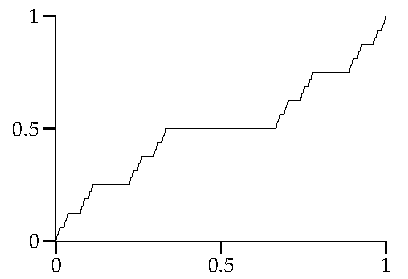
\includegraphics{figures/cantorfunction}
\caption{Cantor function or Devil's staircase (the function $\varphi$ from
the exercise).\label{fig:cantorfunction}}
\end{myfigureht}

\begin{exercise} \label{exercise:allowfiniteseqsinoutermeasure}
Prove that we obtain the same outer measure if we allow both finite and
infinite sequences in
the definition.  That is, define $\mu^*(S) := \inf\, \sum_{j \in I} V(R_j)$
where the infimum is taken over all countable (finite or infinite) sets of
open rectangles $\{ R_j \}_{j\in I}$ such that $S \subset
\bigcup_{j \in I} R_j$.  Prove that for every $S \subset \R^n$,
$\mu^*(S) = m^*(S)$.
\end{exercise}


%%%%%%%%%%%%%%%%%%%%%%%%%%%%%%%%%%%%%%%%%%%%%%%%%%%%%%%%%%%%%%%%%%%%%%%%%%%%%%

\sectionnewpage
\section{The set of Riemann integrable functions }
\label{sec:riemannlebesgue}

\sectionnotes{1 lecture}

\subsection{Oscillation and continuity}

Consider
$S \subset \R^n$ and $f \colon S \to \R$.
Instead of just saying that $f$ is or is not continuous at
a point $x \in S$,
we want to quantify how discontinuous $f$ is 
at $x$.  For every $\delta > 0$, define the \emph{oscillation} of 
$f$ on the $\delta$-ball in subspace topology,
$B_S(x,\delta) = B_{\R^n}(x,\delta) \cap S$, as
\glsadd{not:oscillation}
\begin{equation*}
o(f,x,\delta) :=
{\sup_{y \in B_S(x,\delta)} f(y)}
-
{\inf_{y \in B_S(x,\delta)} f(y)}
= 
\sup_{y_1,y_2 \in B_S(x,\delta)} \bigl(f(y_1)-f(y_2)\bigr) .
\end{equation*}
That is, $o(f,x,\delta)$ is the length of the smallest interval
that contains the image $f\bigl(B_S(x,\delta)\bigr)$.
Clearly $o(f,x,\delta) \geq 0$ and
$o(f,x,\delta) \leq o(f,x,\delta')$ whenever $\delta < \delta'$.
Therefore, the limit as $\delta \to 0$ from the right exists, and
we define the \emph{\myindex{oscillation}} of $f$
at $x$ as
\begin{equation*}
o(f,x) :=
\lim_{\delta \to 0^+}
o(f,x,\delta) =
\inf_{\delta > 0}
o(f,x,\delta) .
\end{equation*}

\begin{prop}
A function
$f \colon S \to \R$ is continuous at $x \in S$ if and only if $o(f,x) = 0$.
\end{prop}

\begin{proof}
First suppose that $f$ is continuous at $x \in S$.  Given any $\epsilon > 0$,
there exists a $\delta > 0$ such that for $y \in B_S(x,\delta)$,
we have $\sabs{f(x)-f(y)} < \epsilon$.  Therefore, if $y_1,y_2 \in
B_S(x,\delta)$, then
\begin{equation*}
f(y_1)-f(y_2) =
\bigl(f(y_1)-f(x)\bigr)-\bigl(f(y_2)-f(x)\bigr) < \epsilon + \epsilon = 2 \epsilon .
\end{equation*}
We take the supremum over $y_1$ and $y_2$
\begin{equation*}
o(f,x,\delta) = 
\sup_{y_1,y_2 \in B_S(x,\delta)} \bigl(f(y_1)-f(y_2)\bigr)
\leq
2 \epsilon .
\end{equation*}
As $o(x,f) \leq o(f,x,\delta) \leq 2\epsilon$, and $\epsilon > 0$ was arbitrary,
$o(x,f) = 0$.

On the other hand suppose $o(x,f) = 0$.  Given any $\epsilon > 0$,
find a $\delta > 0$ such that $o(f,x,\delta) < \epsilon$.  If
$y \in B_S(x,\delta)$, then
\begin{equation*}
\sabs{f(x)-f(y)}
\leq
\sup_{y_1,y_2 \in B_S(x,\delta)} \bigl(f(y_1)-f(y_2)\bigr)
=
o(f,x,\delta) < \epsilon. \qedhere
\end{equation*}
\end{proof}

\begin{prop} \label{prop:seclosed}
Let $S \subset \R^n$ be closed,
$f \colon S \to \R$, and $\epsilon > 0$.
The set $\bigl\{ x \in S : o(f,x) \geq \epsilon \bigr\}$ is closed.
\end{prop}

\begin{proof}
Equivalently, we want to show that
$G = \bigl\{ x \in S : o(f,x) < \epsilon \bigr\}$ is open in the subspace topology.
As $\inf_{\delta > 0} o(f,x,\delta) < \epsilon$, find a $\delta > 0$ such
that
\begin{equation*}
o(f,x,\delta) < \epsilon
\end{equation*}
Take any $\xi \in B_S(x,\nicefrac{\delta}{2})$.  Notice that
$B_S(\xi,\nicefrac{\delta}{2}) \subset B_S(x,\delta)$.  Therefore,
\begin{equation*}
o(f,\xi,\nicefrac{\delta}{2}) =
\sup_{y_1,y_2 \in B_S(\xi,\nicefrac{\delta}{2})} \bigl(f(y_1)-f(y_2)\bigr) 
\leq
\sup_{y_1,y_2 \in B_S(x,\delta)} \bigl(f(y_1)-f(y_2)\bigr) = o(f,x,\delta) <
\epsilon .
\end{equation*}
So $o(f,\xi) < \epsilon$ as well.  As this is true for all $\xi \in
B_S(x,\nicefrac{\delta}{2})$, we get that $G$ is open in the subspace
topology and $S \setminus G$ is closed as claimed.
\end{proof}


\subsection{The set of Riemann integrable functions}

We have seen that continuous functions are Riemann integrable, but we also
know that certain kinds of discontinuities are allowed.
It turns out that as long as the discontinuities happen on a set of measure
zero, the function is integrable, and vice versa.

\begin{thm}[Riemann--Lebesgue]\index{Riemann--Lebesgue theorem}
Let $R \subset \R^n$ be a closed rectangle and $f \colon R \to \R$
a bounded function.  Then $f$ is Riemann integrable if and only if
the set of discontinuities of $f$ is of measure zero (a null set).
\end{thm}

\begin{proof}
Let $S \subset R$ be the set of discontinuities of $f$, that is,
$S = \bigl\{ x \in R : o(f,x) > 0 \bigr\}$.
Suppose $S$ is a measure zero set: $m^*(S) = 0$.
The trick to this proof is to isolate the
bad set into a small set of subrectangles of a partition.  There are only
finitely many subrectangles of a partition, so we will wish to use
compactness.  If $S$ were closed, then it would be compact and we could cover
it by finitely many small rectangles as it is of measure zero.  Unfortunately, $S$
is not closed in general, so we need to work a little harder.

For every $\epsilon > 0$, define
\begin{equation*}
S_\epsilon := \bigl\{ x \in R : o(f,x) \geq \epsilon \bigr\} .
\end{equation*}
By \propref{prop:seclosed}, $S_\epsilon$ is closed and as it is a subset of
$R$,
which is bounded, $S_\epsilon$ is compact.  Furthermore,
$S_\epsilon \subset S$ and $S$ is of measure zero, so $S_\epsilon$ is
measure zero.
Via \propref{mv:prop:compactnull} finitely many open rectangles
$O_1,O_2,\ldots,O_k$ cover $S_\epsilon$ and
$\sum V(O_j) < \epsilon$.  

The set $T = R \setminus ( O_1 \cup \cdots \cup O_k )$ is closed, bounded,
and therefore compact.  Furthermore, $o(f,x) < \epsilon$ for all $x \in T$.
Hence for each $x \in T$, there exists a small closed rectangle
$T_x$ with $x$ in the interior of $T_x$, such that
\begin{equation*}
\sup_{y\in T_x} f(y) - \inf_{y\in T_x} f(y) < 2\epsilon.
\end{equation*}
The interiors of the rectangles $T_x$ cover $T$.  As $T$ is compact,
finitely many such rectangles $T_1, T_2, \ldots, T_m$
cover $T$.

Take the rectangles $T_1,T_2,\ldots,T_m$ and $O_1,O_2,\ldots,O_k$
and construct a partition out of their endpoints.  That is, construct
a partition $P$ of $R$ with subrectangles $R_1,R_2,\ldots,R_p$
such that every $R_j$ is contained in $T_\ell$ for some $\ell$
or the closure of $O_\ell$ for some $\ell$.  Order
the rectangles so that $R_1,R_2,\ldots,R_q$ are those
that are contained in some $T_\ell$, and $R_{q+1},R_{q+2},\ldots,R_{p}$
are the rest.
In particular,
\begin{equation*}
\sum_{j=1}^q V(R_j) \leq V(R)
\qquad \text{and} \qquad
\sum_{j=q+1}^p V(R_j) \leq \epsilon .
\end{equation*}
Let $m_j$ and $M_j$ be the inf and sup
of $f$
over $R_j$ as before.
If $R_j \subset T_\ell$ for some $\ell$, then $(M_j-m_j) < 2 \epsilon$.
Let $B \in \R$ be such that
$\sabs{f(x)} \leq B$ for all $x \in R$, so $(M_j-m_j) < 2B$ over all
rectangles. Then
\begin{equation*}
\begin{split}
U(P,f)-L(P,f)
& =
\sum_{j=1}^p (M_j-m_j) V(R_j)
\\
& =
\left(
\sum_{j=1}^q (M_j-m_j) V(R_j)
\right)
+
\left(
\sum_{j=q+1}^p (M_j-m_j) V(R_j)
\right)
\\
& \leq
\left(
\sum_{j=1}^q 2\epsilon\, V(R_j)
\right)
+
\left(
\sum_{j=q+1}^p 2 B\, V(R_j)
\right)
\\
& \leq
2 \epsilon\, V(R)
+
2B \epsilon = \epsilon \bigl(2\, V(R)+2B\bigr) .
\end{split}
\end{equation*}
We can make the right-hand side as small as we want,
and hence $f$ is integrable.

\medskip

For the other direction, suppose $f$ is Riemann integrable
on $R$.
Let $S$ be the set of discontinuities again.  Consider
the sequence of sets
\begin{equation*}
S_{1/k} = \bigl\{ x \in R : o(f,x) \geq \nicefrac{1}{k} \bigr\}.
\end{equation*}
Fix a $k \in \N$.
Given an $\epsilon > 0$, find a partition $P$ with subrectangles
$R_1,R_2,\ldots,R_p$ such that
\begin{equation*}
U(P,f)-L(P,f) =
\sum_{j=1}^p (M_j-m_j) V(R_j)
< \epsilon
\end{equation*}
Suppose $R_1,R_2,\ldots,R_p$ are ordered so that
the interiors of $R_1,R_2,\ldots,R_{q}$ intersect $S_{1/k}$,
while the interiors of $R_{q+1},R_{q+2},\ldots,R_p$
are disjoint from $S_{1/k}$.  If $x \in R_j \cap S_{1/k}$
and $x$ is in the interior of $R_j$,
%so sufficiently small balls are completely inside $R_j$,
then by definition of $S_{1/k}$ we have
$M_j-m_j \geq \nicefrac{1}{k}$.
Then
\begin{equation*}
\epsilon >
\sum_{j=1}^p (M_j-m_j) V(R_j)
\geq
\sum_{j=1}^q (M_j-m_j) V(R_j)
\geq
\frac{1}{k}
\sum_{j=1}^q V(R_j)
\end{equation*}
In other words,
$\sum_{j=1}^q V(R_j) < k \epsilon$.
Let $G$ be the set of all boundaries of all the subrectangles
of $P$.  The set $G$ is of measure zero (see \exampleref{mv:example:planenull}).
Let $R_j^\circ$ denote the interior of $R_j$, then
\begin{equation*}
S_{1/k} \subset R_1^\circ \cup R_2^\circ \cup \cdots \cup R_q^\circ \cup G .
\end{equation*}
As $G$ can be covered by open rectangles arbitrarily small volume,
$S_{1/k}$ must be of measure zero.  As
\begin{equation*}
S = \bigcup_{k=1}^\infty S_{1/k}
\end{equation*}
and a countable union of measure zero sets is of measure zero, 
$S$ is of measure zero.
\end{proof}

\begin{cor} \label{cor:closednessofriemannintegrable}
Let $R \subset \R^n$ be a closed rectangle.  Let $\sR(R)$ be the set
of Riemann integrable functions on $R$.  Then
\begin{enumerate}[(i)]
\item
$\sR(R)$ is a real algebra:
If $f,g \in \sR(R)$ and $a \in \R$, then $af \in \sR(R)$, $f+g \in \sR(R)$
and $fg \in \sR(R)$.
\item
If $f,g \in \sR(R)$ and
\begin{equation*}
\varphi(x) := \max \bigl\{ f(x) , g(x) \bigr\} ,
\qquad
\psi(x) := \min \bigl\{ f(x) , g(x) \bigr\} ,
\end{equation*}
then $\varphi, \psi \in \sR(R)$.
\item
If $f \in \sR(R)$, then $\sabs{f} \in \sR(R)$, where $\sabs{f}(x) :=
\sabs{f(x)}$.
\item
If $R' \subset \R^m$ is another closed rectangle,
$U \subset \R^n$ and $U' \subset \R^m$ are open sets such that
$R \subset U$ and $R' \subset U'$,
$g \colon U \to U'$ is continuously differentiable, bijective,
$g^{-1}$ is continuously differentiable,
and $f \in \sR(R')$,
then the composition $f \circ g$ is Riemann integrable on $R$.
\end{enumerate}
\end{cor}

The proof is contained in the exercises.

\subsection{Exercises}

\begin{exercise}
Suppose $f \colon (a,b) \times (c,d) \to \R$ is a bounded continuous
function.  Show that the integral of $f$ over $R = [a,b] \times [c,d]$ makes sense
and is uniquely defined.  That is, set $f$ to be anything on the boundary of
$R$ and compute the integral, showing that the values on the boundary are
irrelevant.
\end{exercise}

\begin{exercise}
Suppose $R \subset \R^n$ is a closed rectangle.  Show that $\sR(R)$, the set
of Riemann integrable functions, is an algebra.  That is, show that
if $f,g \in \sR(R)$ and $a \in \R$, then $af \in \sR(R)$, $f+g \in \sR(R)$,
and $fg \in \sR(R)$.
\end{exercise}

\begin{exercise}
Suppose $R \subset \R^n$ is a closed rectangle and
$f \colon R \to \R$ is a bounded function which is zero except on a closed set $E
\subset R$ of measure
zero.  Show that $\int_R f$ exists and compute it.
\end{exercise}

\begin{exercise}
Suppose $R \subset \R^n$ is a closed rectangle and
$f \colon R \to \R$ and
$g \colon R \to \R$ are two Riemann integrable functions.  Suppose $f = g$
except for a closed set $E \subset R$ of measure zero.  Show that $\int_R f = \int_R g$.
\end{exercise}

\begin{samepage}
\begin{exercise}
Suppose $R \subset \R^n$ is a closed rectangle and
$f \colon R \to \R$ is a bounded function.
\begin{enumerate}[a)]
\item
Suppose there exists a closed set $E \subset R$ of measure zero such that
$f|_{R\setminus E}$ is continuous.  Then $f \in \sR(R)$.
\item
Find an example where $E \subset R$ is a set of measure zero
(not closed) such that
$f|_{R\setminus E}$ is continuous and $f \not\in \sR(R)$.
\end{enumerate}
\end{exercise}
\end{samepage}

\begin{exercise}
Suppose $R \subset \R^n$ is a closed rectangle
and $f \colon R \to \R$ and $g \colon R \to \R$ 
are Riemann integrable.
Show that
\begin{equation*}
\varphi(x) := \max \bigl\{ f(x) , g(x) \bigr\} ,
\qquad
\psi(x) := \min \bigl\{ f(x) , g(x) \bigr\} ,
\end{equation*}
are Riemann integrable.
\end{exercise}

\begin{exercise}
Suppose $R \subset \R^n$ is a closed rectangle
and $f \colon R \to \R$ is Riemann integrable.
Show that $\sabs{f}$ is Riemann integrable.
Hint: Define
$f_+(x) := \max \bigl\{ f(x) , 0 \bigr\}$ and
$f_-(x) := \max \bigl\{ -f(x) , 0 \bigr\}$, and then write $\sabs{f}$
in terms of $f_+$ and $f_-$.
\end{exercise}

\begin{exercise}
\leavevmode
\begin{enumerate}[a)]
\item
Suppose $R \subset \R^n$ and
$R' \subset \R^m$ are closed rectangles,
$U \subset \R^n$ and $U' \subset \R^m$ are open sets such that
$R \subset U$ and $R' \subset U'$,
$g \colon U \to U'$ is continuously differentiable, bijective,
$g^{-1}$ is continuously differentiable, and
$f \in \sR(R')$, 
then the composition $f \circ g$ is Riemann integrable on $R$.
\item
Find a counterexample when $g$ is not one-to-one.
Hint: Try $g(x,y) := (x,0)$ and $R=R'=[0,1] \times [0,1]$.
\end{enumerate}
\end{exercise}

\begin{exercise}
Suppose 
$f \colon [0,1]^2 \to \R$ is defined by
\begin{equation*}
f(x,y) :=
\begin{cases}
\frac{1}{kq} & \text{if } x,y \in \Q \text{ and } x = \frac{\ell}{k}
\text{ and } y=\frac{p}{q} \text{ in lowest terms,} \\
0            & \text{else.}
\end{cases}
\end{equation*}
Show that $f \in \sR\bigl({[0,1]}^2\bigr)$.
\end{exercise}

\begin{exercise}
Compute the oscillation $o\bigl(f,(x,y)\bigr)$ for all $(x,y) \in \R^2$
for the function
\begin{equation*}
f(x,y) :=
\begin{cases}
\frac{xy}{x^2+y^2} & \text{if } (x,y) \not= (0,0), \\
0                  & \text{if } (x,y) = (0,0) .
\end{cases}
\end{equation*}
\end{exercise}

\begin{exercise}
Consider the popcorn function $f \colon [0,1] \to \R$,
\begin{equation*}
f(x) :=
\begin{cases}
\frac{1}{q} & \text{if } x \in \Q \text{ and } x = \frac{p}{q}
 \text{ in lowest terms,} \\
0           & \text{else.}
\end{cases}
\end{equation*}
Compute $o(f,x)$ for all $x \in [0,1]$.
\end{exercise}


%%%%%%%%%%%%%%%%%%%%%%%%%%%%%%%%%%%%%%%%%%%%%%%%%%%%%%%%%%%%%%%%%%%%%%%%%%%%%%

\sectionnewpage
\section{Jordan measurable sets}
\label{sec:jordansets}

\sectionnotes{1 lecture}

\subsection{Volume and Jordan measurable sets}

Given a set
$S \subset \R^n$, its \emph{\myindex{characteristic function}}
or \emph{\myindex{indicator function}} $\chi_S \colon \R^n \to \R$
is defined by
\glsadd{not:indicatorfunction}
\begin{equation*}
\chi_S(x) :=
\begin{cases}
1 & \text{if } x \in S, \\
0 & \text{if } x \notin S.
\end{cases}
\end{equation*}
A bounded set $S$ is \emph{\myindex{Jordan measurable}}\footnote{Named after
the French mathematician
\href{https://en.wikipedia.org/wiki/Camille_Jordan}{Marie Ennemond Camille Jordan}
(1838--1922).}
if for some closed rectangle $R$ such that $S \subset R$, the function
$\chi_S$ is Riemann integrable, that is, $\chi_S \in \sR(R)$.
Take two closed rectangles $R$ and $R'$ 
with $S \subset R$ and $S \subset R'$, then $R \cap R'$ is a closed rectangle
also containing $S$.  By \propref{mv:prop:integralsmallerset}
and \exerciseref{mv:zerooutside}, $\chi_S \in \sR(R \cap R')$
and so $\chi_S \in \sR(R')$.  Thus
\begin{equation*}
\int_R \chi_S = \int_{R'} \chi_S = \int_{R \cap R'} \chi_S.
\end{equation*}
We define the
\emph{$n$-dimensional volume}%
\index{n-dimensional volume@$n$-dimensional volume!Jordan measurable set}%
\index{volume} of the
bounded Jordan measurable set $S$ as
\glsadd{not:ndimvolume}
\begin{equation*}
V(S) := \int_R \chi_S ,
\end{equation*}
where $R$ is any closed rectangle containing $S$.

\begin{prop}
A bounded set $S \subset \R^n$ is Jordan measurable if and only if
the boundary $\partial S$ is a measure zero set.
\end{prop}

\begin{proof}
Suppose $R$ is a closed rectangle such that $S$ is
contained in the interior of $R$.
If $x \in \partial S$, then for every $\delta > 0$,
the sets $S \cap B(x,\delta)$ (where $\chi_S$ is 1) and
the sets $(R \setminus S) \cap B(x,\delta)$ (where $\chi_S$ is 0) are
both nonempty.  So $\chi_S$ is not continuous at $x$.
If $x$ is either in the interior of $S$ or in the complement of the closure
$\widebar{S}$, then $\chi_S$ is either identically 1 or identically 0
in a whole neighborhood of $x$ and hence $\chi_S$ is continuous at $x$.
Therefore, the set of discontinuities of $\chi_S$ is precisely the
boundary $\partial S$.  The proposition follows.
\end{proof}

\begin{prop} \label{prop:jordanmeas}
Suppose $S$ and $T$ are bounded Jordan measurable sets.
Then
\begin{enumerate}[(i)]
\item The closure $\widebar{S}$ is Jordan measurable.
\item The interior $S^\circ$ is Jordan measurable.
\item $S \cup T$ is Jordan measurable.
\item $S \cap T$ is Jordan measurable.
\item $S \setminus T$ is Jordan measurable.
\end{enumerate}
\end{prop}

The proof of the proposition is left as an exercise.
Next, we find that the volume that we defined above coincides with the outer
measure we defined above.

\begin{prop}
If $S \subset \R^n$ is Jordan measurable, then $V(S) = m^*(S)$.
\end{prop}

\begin{proof}
Given $\epsilon > 0$,
let $R$ be a closed rectangle that contains $S$.  Let $P$ be a partition
of $R$ such that 
\begin{equation*}
U(P,\chi_S) \leq \left( \int_R \chi_S \right) + \epsilon = V(S) + \epsilon
\qquad \text{and} \qquad
L(P,\chi_S) \geq \left( \int_R \chi_S \right) - \epsilon = V(S)-\epsilon.
\end{equation*}
Let $R_1,R_2,\ldots,R_k$ be all the subrectangles of $P$ such that $\chi_S$ is not
identically zero on each $R_j$.  That is, there is some point $x \in R_j$ such
that $x \in S$.  Let $O_j$ be an open rectangle such that $R_j \subset O_j$
and $V(O_j) < V(R_j) + \nicefrac{\epsilon}{k}$.  Notice that $S \subset
\bigcup_j O_j$.  Then
\begin{equation*}
U(P,\chi_S) = \sum_{j=1}^k V(R_j) > 
\left(\sum_{j=1}^k V(O_j)\right) - \epsilon \geq m^*(S) - \epsilon .
\end{equation*}
As 
$U(P,\chi_S) \leq V(S) + \epsilon$, then
$m^*(S) - \epsilon \leq V(S) + \epsilon$, or in other words
$m^*(S) \leq V(S)$.

Let $R'_1,R'_2,\ldots,R'_\ell$ be all the subrectangles of $P$ such that
$\chi_S$ is identically one on each $R'_j$.  In other words,
these are the subrectangles contained in $S$.
  The interiors
of the subrectangles $R'^\circ_j$ are disjoint and
$V(R'^\circ_j) = V(R'_j)$.  It is easy to see from definition
that 
\begin{equation*}
m^*\Bigl(\bigcup_{j=1}^\ell R'^\circ_j\Bigr)
=
\sum_{j=1}^\ell
V(R'^\circ_j) .
\end{equation*}
Hence
\begin{equation*}
m^*(S) \geq
m^*\Bigl(\bigcup_{j=1}^\ell R'_j\Bigr)
\geq
m^*\Bigl(\bigcup_{j=1}^\ell R'^\circ_j\Bigr)
=
\sum_{j=1}^\ell
V(R'^\circ_j)
=
\sum_{j=1}^\ell
V(R'_j)
=
L(P,f) \geq V(S) - \epsilon .
\end{equation*}
Therefore $m^*(S) \geq V(S)$ as well.
\end{proof}

\subsection{Integration over Jordan measurable sets}

In $\R$ there is only one reasonable type of set to integrate over:
an interval.   In $\R^n$ there are many kinds of sets.  The ones
that work with the Riemann integral are the Jordan measurable sets.

\begin{defn}
Let $S \subset \R^n$ be a bounded Jordan measurable set.
A bounded function $f \colon S \to \R$
is said to be
\emph{\myindex{Riemann integrable on $S$}}\index{integrable on $S$},
or\glsadd{not:integrablefuncR} $f \in \sR(S)$, if for a closed
rectangle $R$ such that $S \subset R$, the function $\widetilde{f} \colon R
\to \R$ defined by
\begin{equation*}
\widetilde{f}(x) :=
\begin{cases}
f(x) & \text{if } x \in S, \\
0 & \text{otherwise},
\end{cases}
\end{equation*}
is in $\sR(R)$.  In this case we write
\glsadd{not:riemannintR}%
\begin{equation*}
\int_S f := \int_R \widetilde{f}.
\end{equation*}
\end{defn}

When $f$ is defined on a larger set and we wish to integrate over $S$, then
we apply the definition to the restriction $f|_S$.  In particular, 
if $f \colon R \to \R$ for a closed rectangle $R$, and $S \subset R$ is
a Jordan measurable subset, then
\begin{equation*}
\int_S f = \int_R f \chi_S .
\end{equation*}

\begin{prop}
If $S \subset \R^n$ is a bounded Jordan measurable set and $f \colon S \to \R$
is a bounded continuous function, then $f$ is integrable on $S$.
\end{prop}

\begin{proof}
Define the function $\widetilde{f}$ as above for some closed rectangle $R$ with $S
\subset R$.  If $x \in R \setminus \widebar{S}$, then $\widetilde{f}$
is identically zero in a neighborhood of $x$.  Similarly if $x$ is in the
interior of $S$, then $\widetilde{f} = f$ on a neighborhood of $x$
and $f$ is continuous at $x$.  Therefore, $\widetilde{f}$ is only ever
possibly discontinuous at $\partial S$, which is a set of measure zero,
and we are finished.
\end{proof}

\subsection{Images of Jordan measurable subsets}

Finally, images of Jordan measurable sets are Jordan measurable under
nice enough mappings.  For simplicity, we assume that the Jacobian
determinant never vanishes.

\begin{prop} \label{prop:imagejordanmeas}
Suppose $U \subset \R^n$ is open and
$S \subset U$ is a closed bounded Jordan measurable set.
Suppose
$g \colon U \to \R^n$ is a one-to-one
continuously differentiable mapping such that
the Jacobian determinant $J_g$ is never zero on $S$.
Then $g(S)$ is bounded and Jordan measurable.
\end{prop}

\begin{proof}
Let $T := g(S)$.  As $S \subset \R^n$ is closed and bounded it is compact.
By 
\volIref{\lemmaref*{vI-lemma:continuouscompact} from volume I}{\lemmaref{lemma:continuouscompact}},
the set
$T$ is also compact and so closed and bounded.
We claim $\partial T \subset g(\partial S)$.  Suppose the claim is proved.
As $S$ is Jordan measurable, then
$\partial S$ is measure zero.  Then  $g(\partial S)$ is measure
zero by \propref{prop:imagenull}.  As $\partial T \subset g(\partial
S)$, then $T$ is Jordan measurable.

It is therefore left to prove the claim.
As $T$ is closed, $\partial T \subset T$.
Suppose $y \in \partial T$, then there must exist an
$x \in S$
such that $g(x) = y$, and by hypothesis $J_g(x) \not= 0$.
We use the inverse function theorem (\thmref{thm:inverse}).  We find 
a neighborhood $V \subset U$ of $x$ and an open set $W$ such that
the restriction $f|_V$ is a one-to-one and onto function from $V$ to $W$
with a continuously differentiable inverse.  In particular, $g(x) = y \in W$.
As $y \in \partial T$, there exists a sequence $\{ y_k \}$ in $W$ with
$\lim y_k = y$ and $y_k \notin T$.  As $g|_V$ is invertible and in
particular has a continuous inverse, there exists
a sequence $\{ x_k \}$ in $V$ such that $g(x_k) = y_k$ and $\lim x_k = x$.
Since $y_k \notin T = g(S)$, clearly $x_k \notin S$.  Since $x \in S$, we
conclude that $x \in \partial S$.  The claim is proved, $\partial T \subset
g(\partial S)$.
\end{proof}

\subsection{Exercises}

\begin{exercise}
Prove \propref{prop:jordanmeas}.
\end{exercise}

\begin{exercise}
Prove that a bounded convex set is Jordan measurable.  Hint: Induction on
dimension.
\end{exercise}

\begin{samepage}
\begin{exercise} \label{exercise:intovertypeIset}
Let $f \colon [a,b] \to \R$ and
$g \colon [a,b] \to \R$ be continuous functions and such that
for all $x \in (a,b)$, $f(x) < g(x)$.  Let
\begin{equation*}
U := \bigl\{ (x,y) \in \R^2 : a < x < b \text{ and } f(x) < y < g(x) \bigr\} .
\end{equation*}
\begin{enumerate}[a)]
\item
Show that $U$ is Jordan measurable.
\item
If $\varphi \colon U \to \R$ is Riemann integrable on $U$, then
\begin{equation*}
\int_U \varphi =
\int_a^b \int_{g(x)}^{f(x)} \varphi(x,y) ~ dy ~ dx .
\end{equation*}
\end{enumerate}
\end{exercise}
\end{samepage}

\begin{exercise}
Let us construct an example of a non-Jordan measurable open set.
Start in one dimension.  Let $\{ r_j \}$ be an enumeration
of all rational numbers in $(0,1)$.  Let $(a_j,b_j)$ be open intervals
such that $(a_j,b_j) \subset (0,1)$ for all $j$, $r_j \in (a_j,b_j)$,
and $\sum_{j=1}^\infty (b_j-a_j) < \nicefrac{1}{2}$.  Now let $U :=
\bigcup_{j=1}^\infty (a_j,b_j)$.
\begin{enumerate}[a)]
\item
Show the open intervals $(a_j,b_j)$ as above actually exist.
\item
Prove $\partial U = [0,1] \setminus U$.
\item
Prove $\partial U$ is not of measure zero, and therefore $U$ is not Jordan measurable.
\item
Show that $W :=
\bigl( U \times (0,2) \bigr) \cup \bigl( (0,1) \times (1,2) \bigr)$
is a connected bounded open set in $\R^2$
that is not Jordan measurable.
\end{enumerate}
\end{exercise}

\begin{exercise}
Suppose $K \subset \R^n$ is a closed measure zero set.
\begin{enumerate}[a)]
\item
If $K$ is bounded, prove that $K$ is Jordan measurable.
\item
If $S \subset \R^n$ is bounded and Jordan measurable, prove that
$S \setminus K$ is Jordan measurable.
\item
Construct a bounded Jordan measurable $S \subset \R^n$
and a bounded $T \subset \R^n$ of measure zero, such that
neither $T$ nor $S \setminus T$ is Jordan measurable.
\end{enumerate}
\end{exercise}

\begin{exercise}
Suppose $U \subset \R^n$ is open and $K \subset U$ is compact.
Find a compact Jordan measurable set $S$ such that $S \subset U$
and $K \subset S^\circ$ ($K$ is in the interior of $S$).
\end{exercise}

\begin{exercise} \label{exercise:closednessofriemannintegrable}
Prove a version of \corref{cor:closednessofriemannintegrable}, replacing all closed
rectangles with bounded Jordan measurable sets.
\end{exercise}

%%%%%%%%%%%%%%%%%%%%%%%%%%%%%%%%%%%%%%%%%%%%%%%%%%%%%%%%%%%%%%%%%%%%%%%%%%%%%%

\sectionnewpage
\section{Green's theorem}
\label{sec:mvgreenstheorem}

\sectionnotes{1 lecture, requires \chapterref{path:chapter}}

One of the most important theorems of analysis in several variables is the
so-called generalized Stokes' theorem, a generalization of the
fundamental theorem of calculus.  The two-dimensional
version is called Green's theorem%
\footnote{Named after the British mathematical physicist
\href{https://en.wikipedia.org/wiki/George_Green_(mathematician)}{George Green}
(1793--1841).}.  We will state the theorem in general, but
we will only prove a special, but important, case.

\begin{defn}
Let $U \subset \R^2$ be a bounded connected open set.
Suppose the boundary
$\partial U$ is a disjoint union of (the images of) finitely many
simple closed piecewise smooth paths such that
every $p \in \partial U$ is in the closure of
$\R^2 \setminus \widebar{U}$.
Then $U$ is called a
\emph{\myindex{bounded domain with piecewise smooth boundary}}%
\index{piecewise smooth boundary}
in $\R^2$.
\end{defn}

The condition about points outside the closure says that locally $\partial U$
separates $\R^2$ into an \myquote{inside} and an \myquote{outside.}  The condition prevents
$\partial U$ from being just a \myquote{cut} inside $U$.  As we travel
along the path in a certain orientation,
there is a well-defined left and a right, and either $U$ is on the left
and the complement of $U$ is on the right, or vice versa.   
The orientation on $U$ is the direction in which we travel along the
paths.  We can switch orientation if needed by reparametrizing the
path.

\begin{defn}
Let $U \subset \R^2$ be a bounded domain with piecewise smooth boundary,
let $\partial U$ be oriented ,
and let $\gamma \colon [a,b] \to \R^2$ be a parametrization of $\partial U$
giving the orientation.  Write $\gamma(t) = \big(x(t),y(t)\bigr)$.
If the vector $n(t) := \bigl(-y'(t),x'(t)\bigr)$ points into the domain,
that is, $\epsilon n(t) + \gamma(t)$ is in $U$ for all small enough
$\epsilon > 0$, then $\partial U$ is
\emph{\myindex{positively oriented}}.  
See \figureref{fig:positiveorient}.
Otherwise it is \emph{\myindex{negatively oriented}}.
\end{defn}

\begin{myfigureht}
\subimport*{figures/}{positiveorient.pdf_t}
\caption{Positively oriented domain (left), and a positively oriented
domain with a hole (right).\label{fig:positiveorient}}
\end{myfigureht}


The vector $n(t)$ turns $\gamma^{\:\prime}(t)$
counterclockwise by $90^\circ$, that is to the left.
When we travel along a positively oriented boundary
in the direction of its orientation,
the domain is \myquote{on our left.}
For example,
if $U$ is a bounded domain with \myquote{no holes,} that is $\partial U$
is connected, then the positive orientation means we are traveling
counterclockwise around $\partial U$.  If we do have \myquote{holes,} then we
travel around them clockwise.

\begin{prop}
Let $U \subset \R^2$ be a bounded domain with piecewise smooth boundary.
Then $U$ is Jordan measurable.
\end{prop}

\begin{proof}
We must show that
$\partial U$ is a null set.  As $\partial U$ is a finite
union of piecewise smooth paths, which 
are finite unions of smooth paths, we need only show that 
a smooth path in $\R^2$ is a null set.
Let $\gamma \colon [a,b] \to \R^2$ be a smooth path.
It is enough to show that
$\gamma\bigl((a,b)\bigr)$ is a null set, as adding 
the points $\gamma(a)$ and $\gamma(b)$,
to a null set still results in a null set.
Define
\begin{equation*}
f \colon (a,b) \times (-1,1) \to \R^2,
\qquad \text{as} \qquad
f(x,y) := \gamma(x) .
\end{equation*}
The set $(a,b) \times \{ 0 \}$ is a null set in $\R^2$ and
$\gamma\bigl((a,b)\bigr) = f\bigl( (a,b) \times \{ 0 \} \bigr)$.
By \propref{prop:imagenull}, 
$\gamma\bigl((a,b)\bigr)$ is a null set in $\R^2$
and so
$\gamma\bigl([a,b]\bigr)$ is a null set, and 
so finally $\partial U$ is a null set.
\end{proof}

\begin{thm}[Green]\index{Green's theorem}
Suppose $U \subset \R^2$ is a bounded domain with piecewise smooth boundary with
the boundary positively oriented.  Suppose $P$ and $Q$ are continuously
differentiable functions defined on some open set that contains the closure
$\widebar{U}$.  Then
\begin{equation*}
\int_{\partial U}
P ~ dx + Q~  dy
=
\int_{U}
\left(\frac{\partial Q}{\partial x} - \frac{\partial P}{\partial y} \right)
.
\end{equation*}
\end{thm}

We stated Green's theorem in general, although we will only prove a special 
version of it.  That is, we will only prove it for a special kind of domain.
The general version follows from the special case 
by application of further geometry, and cutting up the general
domain into smaller domains on which to apply the special case.
We will not prove the general case. 

Let $U \subset \R^2$ be a domain with piecewise smooth boundary.
We say $U$ is of \emph{type I}\index{type I domain}
if there exist numbers
$a < b$, and continuous
functions $f \colon [a,b] \to \R$ and
$g \colon [a,b] \to \R$, such that
\begin{equation*}
U := \{ (x,y) \in \R^2 : a < x < b \text{ and } f(x) < y < g(x) \} .
\end{equation*}
Similarly, $U$ is of \emph{type II}\index{type II domain}
if there exist numbers
$c < d$, and continuous
functions $h \colon [c,d] \to \R$ and
$k \colon [c,d] \to \R$, such that
\begin{equation*}
U := \{ (x,y) \in \R^2 : c < y < d \text{ and } h(y) < x < k(y) \} .
\end{equation*}
Finally, $U \subset \R^2$ is of \emph{type III}\index{type III domain}
if it is both of type I and type II\@.  See \figureref{fig:greenstypes}.

\begin{myfigureht}
\includegraphics{figures/greenstypes}
\caption{Domain types for Green's theorem.\label{fig:greenstypes}}
\end{myfigureht}

Common domains to apply Green's theorem to are rectangles and discs, and
these are type III domains.
We will only prove Green's theorem for type III domains.

\begin{proof}[Proof of Green's theorem for $U$ of type III]
Let $f,g,h,k$ be the functions defined above.
Using \exerciseref{exercise:intovertypeIset},
$U$ is Jordan measurable and as $U$ is of type I\@, then
\begin{equation*}
\begin{split}
\int_U 
\left(- \frac{\partial P}{\partial y} \right)
& =
\int_a^b \int_{g(x)}^{f(x)}
\left(- \frac{\partial P}{\partial y} (x,y) \right)
~ dy ~ dx 
\\
& =
\int_a^b \Bigl(
- P\bigl(x,f(x)\bigr) +
P\bigl(x,g(x)\bigr)
\Bigr) ~ dx
\\
& =
\int_a^b P\bigl(x,g(x)\bigr) ~ dx 
-
\int_a^b P\bigl(x,f(x)\bigr) ~ dx .
\end{split}
\end{equation*}
We integrate $P~dx$ along the boundary.
The one-form $P~dx$ integrates to zero 
along the straight vertical lines in the boundary.  Therefore it is
only
integrated along the top and along the bottom.  As a parameter,
$x$ runs from left to right.  If we use the parametrizations that take $x$
to $\bigl(x,f(x)\bigr)$ and to
$\bigl(x,g(x)\bigr)$ we recognize path integrals above.  However the second
path integral is in the wrong direction; the top should be going right to
left, and so we must switch orientation.
\begin{equation*}
\int_{\partial U} P ~ dx
=
\int_a^b P\bigl(x,g(x)\bigr) ~ dx 
+
\int_b^a P\bigl(x,f(x)\bigr) ~ dx
=
\int_U 
\left(- \frac{\partial P}{\partial y} \right) .
\end{equation*}

Similarly, $U$ is also of type II\@.  The form $Q~dy$ integrates to zero along
horizontal lines.   So
\begin{equation*}
\int_U 
\frac{\partial Q}{\partial x}
=
\int_c^d \int_{k(y)}^{h(y)}
\frac{\partial Q}{\partial x}(x,y)
~ dx ~ dy 
=
\int_a^b \Bigl(
Q\bigl(y,h(y)\bigr) 
-
Q\bigl(y,k(y)\bigr)
\Bigr) ~ dx 
=
\int_{\partial U} Q ~ dy .
\end{equation*}
Putting the two together we obtain
\begin{equation*}
\int_{\partial U} P~ dx + Q ~ dy 
=
\int_{\partial U} P~ dx + \int_{\partial U} Q ~ dy 
=
\int_U 
\Bigl(-\frac{\partial P}{\partial y}\Bigr)
+
\int_U 
\frac{\partial Q}{\partial x}
=
\int_U 
\Bigl(
\frac{\partial Q}{\partial x}
-\frac{\partial P}{\partial y}
\Bigr) . \qedhere
\end{equation*}
\end{proof}

We illustrate the usefulness of Green's theorem on a fundamental result
about harmonic functions.

\begin{example}
Suppose $U \subset \R^2$ is open and
$f \colon U \to \R$ is harmonic, that is, $f$ is twice continuously
differentiable and
$\frac{\partial^2 f}{\partial x^2} +
\frac{\partial^2 f}{\partial y^2} = 0$.
We will prove one of the most fundamental properties of harmonic functions.

Let $D_r := B(p,r)$ be closed disc such that its closure $C(p,r) \subset U$.  Write
$p = (x_0,y_0)$.  We orient
$\partial D_r$ positively.  See \exerciseref{green:balltype3orient}.
Then
\begin{equation*}
\begin{split}
0
& =
\frac{1}{2\pi r}
\int_{D_r}
\left(
\frac{\partial^2 f}{\partial x^2} +
\frac{\partial^2 f}{\partial y^2}
\right)
\\
& 
=
\frac{1}{2\pi r}
\int_{\partial D_r}
- \frac{\partial f}{\partial y} ~ dx + 
\frac{\partial f}{\partial x} ~ dy
\\
&
=
\frac{1}{2\pi r}
\int_0^{2\pi}
\biggl(
- \frac{\partial f}{\partial y} \bigl(x_0+r\cos(t),y_0+r\sin(t)\bigr) \bigl(-r\sin(t)\bigr)
\\
& \hspace{1.2in}
+ \frac{\partial f}{\partial x} \bigl(x_0+r\cos(t),y_0+r\sin(t)\bigr) r\cos(t)
\biggr) ~ dt
\\
&
=
\frac{d}{dr}
\left[
\frac{1}{2\pi}
\int_0^{2\pi}
f\bigl(x_0+r\cos(t),y_0+r\sin(t)\bigr) ~ dt
\right] .
\end{split}
\end{equation*}
Let $g(r) := 
\frac{1}{2\pi}
\int_0^{2\pi}
f\bigl(x_0+r\cos(t),y_0+r\sin(t)\bigr) ~ dt$.  Then $g'(r) = 0$ for all
$r > 0$.
The function is constant for $r >0$ and continuous at $r=0$ (exercise).
Therefore, $g(0) = g(r)$ for all $r > 0$, and
\begin{equation*}
g(r) = g(0) = 
\frac{1}{2\pi}
\int_0^{2\pi}
f\bigl(x_0+0\cos(t),y_0+0\sin(t)\bigr) ~ dt
=
f(x_0,y_0).
\end{equation*}
We
proved the \emph{\myindex{mean value property}} of harmonic functions:
\begin{equation*}
f(x_0,y_0) = 
\frac{1}{2\pi}
\int_0^{2\pi}
f\bigl(x_0+r\cos(t),y_0+r\sin(t)\bigr) ~ dt 
=
\frac{1}{2\pi r}
\int_{\partial D_r} f ~ ds .
\end{equation*}
That is, the value at $p = (x_0,y_0)$ is the average over a circle of any
radius $r$ centered at $(x_0,y_0)$.
\end{example}

\subsection{Exercises}

\begin{exercise} \label{green:balltype3orient}
Prove that a disc $B(p,r) \subset \R^2$ is a type III domain, and prove that
the orientation given by the parametrization $\gamma(t) =
\bigl(x_0+r\cos(t),y_0+r\sin(t)\bigr)$ where $p = (x_0,y_0)$ is the positive
orientation of the boundary $\partial B(p,r)$.
\\
Note: Feel free to use what you know about sine and cosine from calculus.
\end{exercise}

\begin{exercise}
Prove that a convex bounded domain with piecewise smooth boundary
is a type III domain.
\end{exercise}

\begin{exercise}
Suppose $V \subset \R^2$ is a domain with piecewise smooth boundary that is
a type III domain and suppose that $U \subset \R^2$ is a domain such that
$\widebar{V} \subset U$.  Suppose $f \colon U \to \R$ is a twice
continuously differentiable function.  Prove that
$\int_{\partial V}
\frac{\partial f}{\partial x} dx + 
\frac{\partial f}{\partial y} dy = 0$.
\end{exercise}

\begin{samepage}
\begin{exercise}
For a disc $B(p,r) \subset \R^2$, orient the boundary $\partial B(p,r)$
positively.
\begin{enumerate}[a)]
\item
Compute $\displaystyle \int_{\partial B(p,r)} -y ~ dx$.
\item
Compute $\displaystyle \int_{\partial B(p,r)} x ~ dy$.
\item
Compute $\displaystyle \int_{\partial B(p,r)} \frac{-y}{2} ~ dx +
\frac{x}{2} ~ dy$.
\end{enumerate}
\end{exercise}
\end{samepage}

\begin{exercise}
Using Green's theorem show that the area of a triangle with
vertices
$(x_1,y_1)$,
$(x_2,y_2)$,
$(x_3,y_3)$ is
$\frac{1}{2}\sabs{x_1y_2 + x_2 y_3 + x_3 y_1 - y_1x_2 - y_2x_3 - y_3x_1}$.
Hint: See previous exercise.
\end{exercise}

\begin{exercise}
Using the mean value property prove the
\emph{maximum principle}\index{maximum principle!harmonic functions}
for harmonic functions:
Suppose $U \subset \R^2$ is a connected open set and
$f \colon U \to \R$ is harmonic. Prove that
if $f$ attains a maximum at $p \in U$, then $f$ is constant.
\end{exercise}

\begin{exercise}
Let $f(x,y) := \ln \sqrt{x^2+y^2}$.
\begin{enumerate}[a)]
\item
Show $f$ is harmonic where defined.
\item
Show $\lim_{(x,y) \to 0} f(x,y) = -\infty$.
\item
Using a circle $C_r$ of radius
$r$ around the origin, compute $\frac{1}{2\pi r} \int_{\partial C_r} f ds$.
What happens as $r \to 0$?
\item
Why can't you use Green's theorem?
\end{enumerate}
\end{exercise}


%%%%%%%%%%%%%%%%%%%%%%%%%%%%%%%%%%%%%%%%%%%%%%%%%%%%%%%%%%%%%%%%%%%%%%%%%%%%%%

\sectionnewpage
\section{Change of variables}
\label{sec:mvchangeofvars}

\sectionnotes{1 lecture}

In one variable, we have the familiar change of variables
\begin{equation*}
\int_a^b f\bigl(g(x)\bigr) g'(x)~ dx = 
\int_{g(a)}^{g(b)} f(x) ~ dx .
\end{equation*}
The analogue in higher dimensions is quite
a bit more complicated.  The first complication is orientation.  If we use
the definition of integral from this chapter, then we do not have the notion
of $\int_a^b$ versus $\int_b^a$.  We are simply integrating over an
interval $[a,b]$.  With this notation, the change of variables becomes
\begin{equation*}
\int_{[a,b]} f\bigl(g(x)\bigr) \sabs{g'(x)}~ dx = 
\int_{g([a,b])} f(x) ~ dx .
\end{equation*}
In this section we will obtain the several-variable analogue of this form.

Let us remark the role of $\sabs{g'(x)}$ in the formula. 
The integral measures volumes in general, so in one dimension it measures length.
Notice that $\sabs{g'(x)}$ scales the $dx$ and
so it scales the lengths.
If our $g$ is linear, that is, $g(x)=Lx$, then
$g'(x) = L$ and the length of the interval $g([a,b])$ is simply
$\sabs{L}(b-a)$.  That is because $g([a,b])$ is either $[La,Lb]$ or
$[Lb,La]$.  This property holds in higher dimension with $\sabs{L}$ replaced
by the absolute value of the determinant.

\begin{prop} \label{prop:volrectdet}
Suppose $R \subset \R^n$ is a rectangle
and $A \colon \R^n \to \R^n$ is linear.  Then
$A(R)$ is Jordan measurable and $V\bigl(A(R)\bigr) = \sabs{\det (A)} V(R)$.
\end{prop}

\begin{proof}
It is enough to prove for elementary matrices.  The proof is left as an
exercise.
\end{proof}

Let us prove that
absolute value of the Jacobian determinant
$\sabs{J_g(x)} = \babs{\det \bigl(g'(x)\bigr)}$
is the replacement of $\sabs{g'(x)}$ for multiple
dimensions in the change of variables formula.
The following theorem holds in more generality,
but this statement is sufficient for many uses.

\begin{thm}
Suppose $U \subset \R^n$ is open,
$S \subset U$ is a closed bounded Jordan measurable set, and
$g \colon U \to \R^n$ is a one-to-one
continuously differentiable mapping, such that
$J_g$ is never zero on $S$.
Suppose $f \colon g(S) \to \R$ is Riemann integrable.
Then $f \circ g$ is Riemann integrable on $S$ and
\begin{equation*}
\int_{g(S)} f(x) ~ dx = 
\int_S f\bigl(g(x)\bigr) \sabs{J_g(x)} ~ dx .
\end{equation*}
\end{thm}

The set $g(S)$ is Jordan measurable by \propref{prop:imagejordanmeas},
so the left-hand side does make sense.
That the right-hand side makes sense follows by
\corref{cor:closednessofriemannintegrable} (actually
\exerciseref{exercise:closednessofriemannintegrable}).

\begin{proof}
The set $S$ can be covered by finitely many closed rectangles
$P_1,P_2,\ldots,P_k$, whose
interiors do not overlap such that each $P_j \subset U$
(\exerciseref{mv:changeofvarcoverbyrects}).
Proving the theorem for $P_j \cap S$ instead of $S$ is enough.
Define $f(y) := 0$ for all $y \notin g(S)$.
The new $f$ is still Riemann integrable since $g(S)$ is Jordan measurable.
We can now replace the integrals over $S$ with integrals over the whole
rectangle.
We therefore assume that $S$ is equal to a rectangle $R$.

Let $\epsilon > 0$ be given.
For every $x \in R$, let
\begin{equation*}
W_x := \bigl\{ y \in U : \snorm{g'(x)-g'(y)} < \nicefrac{\epsilon}{2} \bigr\} .
\end{equation*}
By \exerciseref{mv:changeofvarWxopen},
$W_x$ is open.
As $x \in W_x$ for every $x$, it is an open cover.
By the Lebesgue covering lemma
(\volIref{\lemmaref*{vI-ms:lebesgue} from volume I}{\lemmaref{ms:lebesgue}}),
there exists a $\delta > 0$ such that
for every $y \in R$, there is an $x$ such that $B(y,\delta) \subset W_x$.
In other words, if $P$ is a rectangle of maximum side length less
than $\frac{\delta}{\sqrt{n}}$ and $y \in P$, then $P \subset
B(y,\delta) \subset W_x$.  By triangle inequality,
$\snorm{g'(\xi)-g'(\eta)} < \epsilon$ for all $\xi, \eta \in P$.

Let $R_1,R_2,\ldots,R_N$ be subrectangles partitioning $R$ such that
the maximum side of every $R_j$ is less than
$\frac{\delta}{\sqrt{n}}$.
We also make sure that the minimum side length is at least
$\frac{\delta}{2\sqrt{n}}$, which we can do if $\delta$ is 
sufficiently small relative to the sides of $R$ (\exerciseref{mv:changeofvarrectside}).

Consider some $R_j$ and some fixed $x_j \in R_j$.
First suppose $x_j=0$, $g(0) = 0$, and $g'(0) = I$.
For any given $y \in R_j$,
apply the fundamental theorem of calculus
to the function $t \mapsto g(ty)$ to find
$g(y) = \int_0^1 g'(ty)y ~dt$.  As the
side of $R_j$ is at most $\frac{\delta}{\sqrt{n}}$,
then $\snorm{y} \leq \delta$.  So
\begin{equation*}
\snorm{g(y)-y} =
\norm{\int_0^1 \bigl(g'(ty) y - y\bigr) ~dt} \leq
\int_0^1 \snorm{g'(ty) y - y} ~dt \leq
\snorm{y} \int_0^1 \snorm{g'(ty) - I} ~dt
\leq
\delta \epsilon .
\end{equation*}
Therefore, $g(R_j) \subset \widetilde{R}_j$, where
$\widetilde{R}_j$ is a rectangle obtained from
$R_j$ by extending by
$\delta \epsilon$ on all sides.  See \figureref{changeofvarssq:fig}.

\begin{myfigureht}
\subimport*{figures/}{changeofvarssq.pdf_t}
\caption{Image of $R_j$ under $g$ lies inside
$\widetilde{R}_j$.  A sample point $y \in R_j$ (on the boundary of $R_j$ in fact) is marked
and $g(y)$ must lie within with a radius of $\delta\epsilon$
(also marked).\label{changeofvarssq:fig}}
\end{myfigureht}


If the sides of $R_j$ are $s_1,s_2,\ldots,s_n$, then
$V(R_j) = s_1 s_2 \cdots s_n$.   Recall $\delta \leq 2\sqrt{n} \, s_j$.
Thus,
\begin{equation*}
\begin{split}
V(\widetilde{R}_j) & =
(s_1+2\delta \epsilon )
(s_2+2\delta \epsilon )
\cdots
(s_n+2\delta \epsilon )
\\
& \leq
(s_1+4 \sqrt{n}\,s_1 \epsilon )
(s_2+4 \sqrt{n}\,s_2 \epsilon )
\cdots
(s_n+4 \sqrt{n}\,s_n \epsilon )
\\
& =
s_1 (1+4 \sqrt{n}\, \epsilon )
\,
s_2 (1+4 \sqrt{n}\, \epsilon )
\cdots
s_n (1+4 \sqrt{n}\, \epsilon )
=
V(R_j) {(1+4\sqrt{n} \, \epsilon)}^n .
\end{split}
\end{equation*}
In other words,
\begin{equation*}
V\bigl(g(R_j)\bigr) \leq V(\widetilde{R}_j) \leq V(R_j) {(1+4\sqrt{n} \, \epsilon)}^n .
\end{equation*}
Next, suppose $A := g'(0)$ is not necessarily the identity.
Write $g = A \circ \widetilde{g}$ where $\widetilde{g}'(0) = I$.
By \propref{prop:volrectdet},
$V\bigl(A(R_j)\bigr) = \sabs{\det(A)}V(R_j)$, and hence
\begin{equation*}
\begin{split}
V\bigl(g(R_j)\bigr) & \leq
\sabs{\det(A)} V(R_j) {(1+4\sqrt{n} \, \epsilon)}^n \\
& =
\sabs{J_g(0)} V(R_j) {(1+4\sqrt{n} \, \epsilon)}^n .
\end{split}
\end{equation*}
Translation does not change volume, and therefore
for every $R_j$, and $x_j \in R_j$, including when $x_j \not= 0$ and $g(x_j)
\not= 0$, we find
\begin{equation*}
V\bigl(g(R_j)\bigr) \leq
\sabs{J_g(x_j)} V(R_j) {(1+4\sqrt{n} \, \epsilon)}^n .
\end{equation*}

Write $f$ as
$f = f_+ - f_-$ for two nonnegative Riemann integrable
functions $f_+$ and $f_-$:
\begin{equation*}
f_+(x) := \max \{ f(x) , 0 \}, \qquad
f_-(x) := \max \{ -f(x) , 0 \} .
\end{equation*}
So, if we prove the theorem for a nonnegative $f$,
we obtain the theorem for arbitrary $f$.
Therefore, suppose that 
$f(y) \geq 0$ for all $y \in R$.

For a small enough
$\delta > 0$, we have
\begin{equation*}
\begin{split}
\epsilon + \int_R f\bigl(g(x)\bigr) \sabs{J_g(x)} ~ dx
& \geq
\sum_{j=1}^N \biggl(\sup_{x \in R_j} f\bigl(g(x)\bigr) \sabs{J_g(x)} \biggr) V(R_j)
\\
& \geq
\sum_{j=1}^N \biggl(\sup_{x \in R_j} f\bigl(g(x)\bigr) \biggr) \sabs{J_g(x_j)} V(R_j)
\\
& \geq
\sum_{j=1}^N \biggl(\sup_{y \in g(R_j)} f(y) \biggr)
V\bigl(g(R_j)\bigr)
\frac{1}{{(1+4\sqrt{n} \, \epsilon)}^n}
\\
& \geq
\sum_{j=1}^N \left(\int_{g(R_j)}f(y) ~dy \right)
\frac{1}{{(1+4\sqrt{n} \, \epsilon)}^n}
\\
& =
\frac{1}{{(1+4\sqrt{n} \, \epsilon)}^n}
\int_{g(R)} f(y) ~dy .
\end{split}
\end{equation*}
The last equality follows because the overlaps of the rectangles
are their boundaries, which are of measure zero, and hence the image
of their boundaries is also measure zero.
Let $\epsilon$ go to zero to find
\begin{equation*}
\int_R f\bigl(g(x)\bigr) \sabs{J_g(x)} ~ dx \geq \int_{g(R)} f(y) ~dy .
\end{equation*}
By adding this result for several rectangles covering an $S$ we obtain the
result for an arbitrary bounded Jordan measurable $S \subset U$,
and nonnegative integrable function $f$:
\begin{equation*}
\int_S f\bigl(g(x)\bigr) \sabs{J_g(x)} ~ dx \geq \int_{g(S)} f(y) ~dy .
\end{equation*}

Recall that $g^{-1}$ exists and $g^{-1}\bigl(g(S)\bigr) = S$.
Also $1 = J_{g\circ g^{-1}} = J_g(g^{-1}(y))J_{g^{-1}}(y)$ for $y \in g(S)$.
So
\begin{equation*}
\begin{split}
\int_{g(S)} f(y) ~ dy
& =
\int_{g(S)} f\bigl(g\bigl(g^{-1}(y)\bigr)\bigr)
\sabs{J_g\bigl(g^{-1}(y)\bigr)} \, \sabs{J_{g^{-1}}(y)} ~ dy
\\
& \geq
\int_{g^{-1}(g(S))} f\bigl(g(x)\bigr) \sabs{J_g(x)} ~ dx
=
\int_{S} f\bigl(g(x)\bigr) \sabs{J_g(x)} ~ dx .
\end{split}
\end{equation*}

The conclusion of the theorem holds
for all nonnegative $f$ and as we
mentioned above, it thus holds for all Riemann integrable $f$.
\end{proof}

\subsection{Exercises}

\begin{exercise}
Prove \propref{prop:volrectdet}.
\end{exercise}

\begin{exercise} \label{mv:changeofvarcoverbyrects}
Suppose $U \subset \R^n$ is open
and $S \subset U$ is a closed bounded Jordan measurable set.
Show that there exist finitely many closed bounded rectangles
$P_1,P_2, \ldots, P_k$ such that $P_j \subset U$,
$S \subset P_1 \cup P_2 \cup \cdots \cup P_k$, and
the interiors are mutually disjoint, that is
$P_j^\circ \cap P^\circ_\ell = \emptyset$ whenever $j \not= \ell$.
\end{exercise}

\begin{exercise} \label{mv:changeofvarWxopen}
Suppose $U \subset \R^n$ is open, $x \in U$,
and $g \colon U \to \R^n$ is a continuously differentiable mapping.
For every $\epsilon > 0$, show that
\begin{equation*}
W_x := \bigl\{ y \in U : \snorm{g'(x)-g'(y)} < \nicefrac{\epsilon}{2} \bigr\}
\end{equation*}
is an open set.
\end{exercise}

\begin{exercise} \label{mv:changeofvarrectside}
Suppose $R \subset \R^n$ is a closed bounded rectangle.
Show that if $\delta' > 0$ is sufficiently small relative
to the sides of $R$, then $R$ can be partitioned
into subrectangles where each side of every subrectangle
is between $\frac{\delta'}{2}$ and $\delta'$.
\end{exercise}

\begin{exercise}
Prove the following version of the theorem:
\emph{Suppose $f \colon \R^n \to \R$ is a Riemann integrable
compactly supported function.  Suppose $K \subset \R^n$
is the support of $f$, $S$ is a compact set,
and $g \colon \R^n \to \R^n$ is
a function that when restricted to a neighborhood $U$ of
$S$ is one-to-one and continuously differentiable,
$g(S) = K$ and $J_g$ is never zero on $S$ (in the formula 
assume $J_g(x) = 0$ if $g$ not differentiable at $x$, that is when $x \notin
U$).  Then}
\begin{equation*}
\int_{\R^{n}} f(x) ~ dx = 
\int_{\R^n} f\bigl(g(x)\bigr) \sabs{J_g(x)} ~ dx .
\end{equation*}
\end{exercise}

\begin{exercise}
Prove the following version of the theorem:
\emph{Suppose $S \subset \R^n$ is an open bounded Jordan measurable set,
$g \colon S \to \R^n$ is a one-to-one
continuously differentiable mapping such that
$J_g$ is never zero on $S$, and such that $g(S)$ is bounded and
Jordan measurable (it is also open).
Suppose $f \colon g(S) \to \R$ is Riemann
integrable.  Then $f \circ g$ is Riemann integrable on $S$ and}
\begin{equation*}
\int_{g(S)} f(x) ~ dx = 
\int_S f\bigl(g(x)\bigr) \sabs{J_g(x)} ~ dx .
\end{equation*}
Hint: Write $S$ as an increasing union of closed bounded Jordan measurable
sets, then apply the theorem of the section to those.  Then prove that you
can take the limit.
\end{exercise}


%%%%%%%%%%%%%%%%%%%%%%%%%%%%%%%%%%%%%%%%%%%%%%%%%%%%%%%%%%%%%%%%%%%%%%%%%%%%%%

% Approximating functions chapter
%%%%%%%%%%%%%%%%%%%%%%%%%%%%%%%%%%%%%%%%%%%%%%%%%%%%%%%%%%%%%%%%%%%%%%%%%%%%%%
%%%%%%%%%%%%%%%%%%%%%%%%%%%%%%%%%%%%%%%%%%%%%%%%%%%%%%%%%%%%%%%%%%%%%%%%%%%%%%
%%%%%%%%%%%%%%%%%%%%%%%%%%%%%%%%%%%%%%%%%%%%%%%%%%%%%%%%%%%%%%%%%%%%%%%%%%%%%%

\chapter{Functions as Limits} \label{approx:chapter}

%%%%%%%%%%%%%%%%%%%%%%%%%%%%%%%%%%%%%%%%%%%%%%%%%%%%%%%%%%%%%%%%%%%%%%%%%%%%%%

\section{Complex numbers}
\label{sec:complexnums}

\sectionnotes{half a lecture}

\subsection{The complex plane}

In this chapter we consider approximation of functions, or in other words
functions as limits of sequences and series.
We will extend some results we already saw to a somewhat more
general setting, and we will look at some completely new results.
In particular, we consider complex-valued functions.
We gave complex numbers as examples before, but
let us start from scratch and properly define the complex number field.

A complex number is just a pair $(x,y) \in \R^2$ on which we define
multiplication (see below).
We call the set the \emph{complex numbers}\index{complex number}
and denote it by $\C$.
We identify $x \in \R$ with $(x,0) \in \C$.
The $x$-axis is then called the \emph{\myindex{real axis}} and the $y$-axis is
called the \emph{\myindex{imaginary axis}}.  The set $\C$ is sometimes called the
\emph{\myindex{complex plane}}.

Define:
\begin{align*}
& (x,y) + (s,t) := (x+s,y+t) , \\
& (x,y) (s,t) := (xs-yt,xt+ys) .
\end{align*}
Under the identification above, we have $0 = (0,0)$ and $1 = (1,0)$.  These
two operations make the plane into a field (exercise).

We write a complex number $(x,y)$ as $x+iy$, where we
define\footnote{Note that engineers use $j$ instead of $i$.}
\glsadd{not:imaginary}
\begin{equation*}
i := (0,1) .
\end{equation*}
Notice that $i^2 = (0,1)(0,1) = (0-1,0+0) = -1$.
That is, $i$ is a solution to the polynomial equation
\begin{equation*}
z^2+1=0 .
\end{equation*}
From now on, we will not use the notation $(x,y)$ and use only $x+iy$.
See \figureref{fig:complexplane}.
\begin{myfigureht}
\includegraphics{figures/complexplane}
\caption{The points $1$, $i$, $x$, $iy$, and $x+iy$ in the complex
plane.\label{fig:complexplane}}
\end{myfigureht}

We generally use $x,y,r,s,t$ for real values and $z,w,\xi,\zeta$
for complex values, although that is not a hard and fast rule.  In
particular, $z$ is often used as a third real variable in $\R^3$.

\begin{defn}
Suppose $z= x+iy$.
We call $x$ 
the \emph{\myindex{real part}} of $z$, and 
we call $y$
the \emph{\myindex{imaginary part}} of $z$.  We write
\glsadd{not:realpart}\glsadd{not:imagpart}
\begin{equation*}
\Re\, z := x , \qquad
\Im\, z := y .
\end{equation*}
Define 
\glsadd{not:conj}
\emph{\myindex{complex conjugate}} as
\begin{equation*}
\bar{z} := x-iy ,
\end{equation*}
and define \emph{\myindex{modulus}} as
\glsadd{not:modulus}
\begin{equation*}
\sabs{z} := \sqrt{x^2+y^2} .
\end{equation*}
\end{defn}

Modulus is the complex analogue of the absolute value and
has similar properties.
For example,
$\sabs{zw} = \sabs{z} \, \sabs{w}$ (exercise).
The complex conjugate is a reflection of the plane across the real axis.
The real numbers are precisely those numbers for which the imaginary
part $y=0$.  In particular, they are precisely those numbers which satisfy
the equation
\begin{equation*}
z = \bar{z} .
\end{equation*}

As $\C$ is really $\R^2$, we let the metric on $\C$ be the standard
euclidean metric on $\R^2$.
In particular,
\begin{equation*}
\sabs{z} = d(z,0) , \qquad 
\text{and also} \qquad 
\sabs{z-w} = d(z,w) .
\end{equation*}
So the topology on $\C$ is
the same exact topology as the standard topology on $\R^2$
with the euclidean metric,
and $\sabs{z}$ is equal to the euclidean norm on $\R^2$.
Importantly, since $\R^2$ is a complete metric space, then
so is $\C$.
As $\sabs{z}$ is the euclidean norm on $\R^2$, we have the
\emph{triangle inequality}\index{triangle inequality!complex numbers}
of both flavors:
\begin{equation*}
\sabs{z+w} \leq \sabs{z}+\sabs{w} \qquad \text{and} \qquad
\big\lvert \sabs{z}-\sabs{w} \big\rvert \leq \sabs{z-w} .
\end{equation*}

The complex conjugate and the modulus are even more intimately related:
\begin{equation*}
\sabs{z}^2 =
x^2+y^2 =
(x+iy)(x-iy) =
z \bar{z} .
\end{equation*}

\begin{remark}
There is no natural ordering on the complex numbers.
In particular,
no ordering that makes the complex numbers into an ordered field.
Ordering is one of the things we lose when we go from real to complex
numbers.
\end{remark}

\subsection{Complex numbers and limits}

It is not hard to show that the algebraic operations are
continuous.  This is because convergence in 
$\R^2$ is the same as convergence for each component and we already know
that the real algebraic operations are continuous.  For example,
write $z_n = x_n + i\,y_n$ and
$w_n = s_n + i\,t_n$, and suppose that
$\lim \, z_n = z = x+i\,y$ and $\lim \, w_n = w = s+i\,t$.
Let us show
\begin{equation*}
\lim_{n\to\infty} z_n w_n = zw .
\end{equation*}
First,
\begin{equation*}
z_n w_n = (x_ns_n-y_nt_n) + i(x_nt_n+y_ns_n) .
\end{equation*}
The topology on $\C$ is the same as on $\R^2$, and so
$x_n \to x$, $y_n \to y$, $s_n \to s$, and $t_n \to t$.
Hence,
\begin{equation*}
\lim_{n\to\infty} (x_ns_n-y_nt_n) = xs-yt \qquad \text{and} \qquad
\lim_{n\to\infty} (x_nt_n+y_ns_n) = xt+ys .
\end{equation*}
As
$(xs-yt)+i(xt+ys) = zw$, then
\begin{equation*}
\lim_{n\to\infty} z_n w_n = zw .
\end{equation*}

Similarly the modulus and the complex conjugate are continuous functions.  We
leave the proof of the following proposition as an exercise.

\begin{prop} \label{prop:continuityofcomplex}
Suppose $\{ z_n \}$, $\{ w_n \}$ are sequences of complex numbers converging
to $z$ and $w$ respectively.  Then
\begin{enumerate}[(i)]
\item
$\displaystyle \lim_{n\to \infty} z_n + w_n = z + w$.
\item
$\displaystyle \lim_{n\to \infty} z_n w_n = z w$.
\item
Assuming $w_n \not= 0$ for all $n$ and $w\not= 0$,
$\displaystyle \lim_{n\to \infty} \frac{z_n}{w_n} = \frac{z}{w}$.
\item
$\displaystyle \lim_{n\to \infty} \sabs{z_n} = \sabs{z}$.
\item
$\displaystyle \lim_{n\to \infty} \bar{z}_n = \bar{z}$.
\end{enumerate}
\end{prop}

As we have seen above, convergence in $\C$ is the same as convergence in
$\R^2$.  In particular, a sequence in $\C$ converges if and only if
the real and imaginary parts converge.  Therefore, feel free to apply
everything you have learned about convergence in $\R^2$, as well as
applying results about real numbers to the real and imaginary parts.

We also need convergence of complex series.  Let $\{ z_n \}$ be a
sequence of complex
numbers. The series
\begin{equation*}
\sum_{n=1}^\infty z_n
\end{equation*}
\emph{converges}\index{converges!complex series} if the limit of partial sums converges, that is, if
\begin{equation*}
\lim_{k\to\infty} \sum_{n=1}^k z_n \qquad \text{exists.}
\end{equation*}
As before, we sometimes write $\sum z_n$ for the series.
A series \emph{converges absolutely}\index{converges
absolutely!complex series} if $\sum \sabs{z_n}$ converges.

We say a series
is \emph{Cauchy}\index{Cauchy!complex series}
if the sequence of partial sums is Cauchy.  The following two
propositions have essentially the same proofs as for real series and we
leave them as exercises.

\begin{prop} \label{prop:cachysercomplex}
The complex series $\sum z_n$ is Cauchy if for every $\epsilon > 0$, 
there exists an $M \in \N$ such that for every $n \geq M$
and every $k > n$, we have
\begin{equation*}
\abs{ \sum_{j={n+1}}^k z_j }
< \epsilon .
\end{equation*}
\end{prop}

\begin{prop} \label{prop:absconvmeansconv}
If a complex series $\sum z_n$ converges absolutely, then it converges.
\end{prop}

The series $\sum \sabs{z_n}$ is a real series.  All the
convergence tests (ratio test, root test, etc.)\ that talk about
absolute convergence work with the numbers $\sabs{z_n}$, that is, they
are really talking about convergence of series of nonnegative real
numbers.
You
can directly apply these tests
them without needing to reprove anything for complex
series.

\subsection{Complex-valued functions}

When we deal with complex-valued functions
$f \colon X \to \C$, what we often do is to write
$f = u+i\,v$ for real-valued functions $u \colon X \to \R$ and $v \colon X \to
\R$.

Suppose we wish to integrate
$f \colon [a,b] \to \C$.  We write
$f = u+i\,v$ for real-valued $u$ and $v$.
We say that $f$ is \emph{Riemann integrable}\index{Riemann
integrable!complex-valued function}
if $u$ and $v$ are Riemann
integrable, and in this case we define
\begin{equation*}
\int_a^b f := \int_a^b u + i \int_a^b v .
\end{equation*}
We make the same definition for every other type of integral (improper,
multivariable, etc.).

Similarly when we differentiate, write $f \colon [a,b] \to \C$ as
$f = u+i\,v$.  Thinking of $\C$ as $\R^2$ we say that $f$ is differentiable
if $u$ and $v$ are differentiable.  For a function valued in $\R^2$, the derivative
was represented by a vector in $\R^2$.  Now a vector in $\R^2$ is a complex
number.  In other words,
we write
the
\emph{derivative}\index{derivative!complex-valued function}
as
\glsadd{not:mvder}
\begin{equation*}
f'(t) := u'(t) + i \, v'(t) .
\end{equation*}
The linear operator representing the derivative is the multiplication by
the complex number $f'(t)$, so nothing is lost in this identification.


\subsection{Exercises}

\begin{exercise}
Check that $\C$ is a field.
\end{exercise}

\begin{exercise}
Prove that for $z,w \in \C$, we have
$\sabs{zw} = \sabs{z} \, \sabs{w}$.
\end{exercise}

\begin{exercise}
Finish the proof of \propref{prop:continuityofcomplex}.
\end{exercise}

\begin{exercise}
Prove \propref{prop:cachysercomplex}.
\end{exercise}

\begin{exercise}
Prove \propref{prop:absconvmeansconv}.
\end{exercise}

\begin{samepage}
\begin{exercise}
Considering the definition of complex multiplication, given $x +iy$
define the matrix
$\left[ \begin{smallmatrix} x & -y \\ y & x \end{smallmatrix} \right]$.
Prove that
\begin{enumerate}[a)]
\item
The action of this matrix on a vector $(s,t)$ is the same
as the action of multiplying $(x+iy)(s+it)$.
\item
Multiplying two such matrices is the same multiplying the underlying complex
numbers and then finding the corresponding matrix for the product.
In other words, we can think of the field $\C$ as also a subset of
the 2-by-2 matrices.
\item
Show that 
$\left[ \begin{smallmatrix} x & -y \\ y & x \end{smallmatrix} \right]$
has eigenvalues $x+iy$ and $x-iy$.  Recall that $\lambda$ is
an eigenvalue of a matrix $A$ if $A-\lambda I$ (a complex matrix in our case)
is not invertible, or in other words
if it has linearly dependent rows: That is, one row is a (complex) multiple
of the other
\end{enumerate}
\end{exercise}
\end{samepage}

\begin{exercise}
Prove the Bolzano--Weierstrass theorem for complex sequences.
Suppose $\{ z_n \}$ is a bounded sequence of complex numbers, that
is, there exists an $M$ such that $\sabs{z_n} \leq M$ for all $n$.  Prove
that there exists a subsequence $\{ z_{n_k} \}$ that converges to some $z
\in \C$.
\end{exercise}

\begin{exercise}
\leavevmode
\begin{enumerate}[a)]
\item
Prove that there is no simple mean value theorem for complex-valued
functions:  Find a differentiable function $f \colon [0,1] \to \C$ such that
$f(0) = f(1) = 0$, but $f'(t) \not= 0$ for all $t \in [0,1]$.
\item
However, there is a weaker form of the mean value theorem as there is for vector-valued
functions.  Prove: If $f \colon [a,b] \to \C$ is continuous and differentiable in
$(a,b)$, and for some $M$, $\sabs{f'(x)} \leq M$ for all $x \in (a,b)$, then
$\sabs{f(b)-f(a)} \leq M \sabs{b-a}$.
\end{enumerate}
\end{exercise}

\begin{exercise}
Prove that there is no simple mean value theorem for integrals
for complex-valued
functions:  Find a continuous function $f \colon [0,1] \to \C$ such that
$\int_0^1 f = 0$ but $f(t) \not= 0$ for all $t \in [0,1]$.
\end{exercise}


%%%%%%%%%%%%%%%%%%%%%%%%%%%%%%%%%%%%%%%%%%%%%%%%%%%%%%%%%%%%%%%%%%%%%%%%%%%%%%

\sectionnewpage
\section{Swapping limits}
\label{sec:swaplim}

\sectionnotes{2 lectures}

\subsection{Continuity}

Let us get back to swapping limits and expand on
\volIref{\chapterref*{vI-fs:chapter} of volume I}{\chapterref{fs:chapter}}.
Let $\{ f_n \}$ be a sequence
of functions $f_n \colon X \to Y$ for a set $X$ and a metric space $Y$.
Let $f \colon X \to Y$ be a
function and for every $x \in X$ suppose that
\begin{equation*}
f(x) = \lim_{n\to \infty} f_n(x) .
\end{equation*}
We say the sequence $\{ f_n \}$
\emph{\myindex{converges pointwise}}\index{pointwise convergence} to $f$.

For $Y=\C$, a series
\emph{converges pointwise}\index{converges pointwise!complex series}\index{pointwise convergence!complex series} if
for every $x \in X$, we have
\begin{equation*}
f(x) = \lim_{n\to \infty} \sum_{k=1}^n f_k(x) =
\sum_{k=1}^\infty f_k(x) .
\end{equation*}

\medskip

The question is:
If $f_n$ are all continuous, is $f$ continuous?  Differentiable?
Integrable?  What are the derivatives or integrals of $f$?

For example, for continuity of the pointwise limit of a sequence $\{ f_n
\}$, we are asking if
\begin{equation*}
\lim_{x\to x_0} \lim_{n\to\infty} f_n(x)
\overset{?}{=}
\lim_{n\to\infty} \lim_{x\to x_0} f_n(x) .
\end{equation*}
We don't even a priory know if both sides exist, let alone if they are equal each other.

\begin{example}
The functions $f_n \colon \R \to \R$,
\begin{equation*}
f_n(x) := \frac{1}{1+nx^2},
\end{equation*}
are continuous and converge pointwise to the discontinuous function
\begin{equation*}
f(x) := 
\begin{cases}
1 & \text{if } x=0, \\
0 & \text{else.}
\end{cases}
\end{equation*}
\end{example}

So pointwise convergence is not enough to preserve continuity (nor even
boundedness).  For that, we need uniform convergence.

Let $f_n \colon X \to Y$ be functions.  Then
$\{f_n\}$ \emph{\myindex{converges uniformly}}\index{uniform convergence}
to $f$ if
for every $\epsilon > 0$, there exists an $M$ such that
for all $n \geq M$ and all $x \in X$, we have
\begin{equation*}
d\bigl(f_n(x),f(x)\bigr) < \epsilon .
\end{equation*}

A series $\sum f_n$ of complex-valued functions converges uniformly if the sequence of
partial sums converges uniformly, that is for every $\epsilon > 0$
there exists an $M$ such that
for all $n \geq M$ and all $x \in X$
\begin{equation*}
\abs{\left(\sum_{k=1}^n f_k(x)\right)-f(x)} < \epsilon .
\end{equation*}

The simplest property preserved by uniform convergence is
boundedness.  We leave the proof of the following proposition as an
exercise.  It is almost identical to the proof for real-valued functions.

\begin{prop} \label{prop:uniformconvbounded}
Let $X$ be a set and $(Y,d)$ a metric space.
If $f_n \colon X \to Y$ are bounded functions and converge uniformly to $f
\colon X \to Y$, then $f$ is bounded.
\end{prop}

If $X$ is a set and $(Y,d)$ is a metric space, then a sequence $f_n \colon X
\to Y$ is \emph{\myindex{uniformly Cauchy}} if for every $\epsilon > 0$, there is an $M$ such that
for all $n, m \geq M$ and all $x \in X$, we have
\begin{equation*}
d\bigl(f_n(x),f_m(x)\bigr) < \epsilon .
\end{equation*}
The notion is the same as for real-valued functions.
The proof of the following proposition is
again essentially the same as in that setting and
is left as an exercise.

\begin{prop} \label{prop:unifcauchymetric}
Let $X$ be a set, $(Y,d)$ be a metric space, and
$f_n \colon X \to Y$ be functions.
If $\{ f_n \}$ converges uniformly,
then $\{f_n\}$ is uniformly Cauchy.  Conversely, if 
$\{f_n\}$ is uniformly Cauchy and $(Y,d)$ is Cauchy-complete,
then $\{f_n\}$ converges uniformly.
\end{prop}

For $f \colon X \to \C$, we write\glsadd{not:uniformnorm}
\begin{equation*}
\snorm{f}_u := \sup_{x \in X} \sabs{f(x)} .
\end{equation*}
We call $\snorm{\cdot}_u$
the \emph{\myindex{supremum norm}} or \emph{\myindex{uniform norm}}.
Then a sequence of functions
$f_n \colon X \to \C$ converges uniformly to $f \colon X \to \C$ if and only if
\begin{equation*}
\lim_{n\to \infty} \snorm{f_n-f}_u = 0 .
\end{equation*}

The supremum norm satisfies the triangle inequality: For every $x \in X$,
\begin{equation*}
\sabs{f(x)+g(x)} \leq
\sabs{f(x)}+\sabs{g(x)} \leq
\snorm{f}_u+\snorm{g}_u .
\end{equation*}
Take a supremum on the left to get
\begin{equation*}
\snorm{f+g}_u \leq
\snorm{f}_u+\snorm{g}_u .
\end{equation*}

For a compact metric space $X$,
the uniform norm is a norm on the vector space $C(X,\C)$.
We leave it as an exercise.
While we will not need it, $C(X,\C)$ is in fact a complex
vector space, that is, in the definition of a vector space we can replace
$\R$ with $\C$.
Convergence in the metric space $C(X,\C)$ is
uniform convergence.

We will study a couple of types of series of functions, and
a useful test for uniform convergence of a series is the 
so-called \emph{\myindex{Weierstrass $M$-test}}.

\begin{thm}[\myindex{Weierstrass $M$-test}] \label{thm:weiermtest}
Let $X$ be a set.
Suppose $f_n \colon X \to \C$ are functions and $M_n > 0$ numbers such
that
\begin{equation*}
\sabs{f_n(x)}\leq M_n \quad \text{for all } x \in X,
\qquad \text{and} \qquad
\sum_{n=1}^\infty M_n
\quad \text{converges}.
\end{equation*}
Then
\begin{equation*}
\sum_{n=1}^\infty f_n(x)
\quad \text{converges uniformly}.
\end{equation*}
\end{thm}

Another way to state the theorem is to say that if
$\sum \snorm{f_n}_u$ converges, then $\sum f_n$ converges uniformly.
Note that the converse of this theorem is not true.
Also note that applying the theorem to $\sum \sabs{f_n(x)}$ gives that
a series satisfying the $M$-test also converges uniformly, so the series converges both absolutely
and uniformly.

\begin{proof}
Suppose $\sum M_n$ converges.  Given $\epsilon > 0$,
we have that the partial sums of $\sum M_n$ are Cauchy so
there is an $N$ such that for all $m, n \geq N$ with $m \geq n$, we have
\begin{equation*}
\sum_{k=n+1}^m M_k < \epsilon .
\end{equation*}
We estimate a Cauchy difference of the partial
sums of the functions
\begin{equation*}
\abs{\sum_{k=n+1}^m f_k(x)} \leq
\sum_{k=n+1}^m \sabs{f_k(x)} \leq
\sum_{k=n+1}^m M_k < \epsilon .
\end{equation*}
We are done by \propref{prop:cachysercomplex}.
\end{proof}

\begin{example} \label{example:sinnsqfourier}
The series
\begin{equation*}
\sum_{n=1}^\infty \frac{\sin(nx)}{n^2}
\end{equation*}
converges uniformly on $\R$.  See \figureref{fig:fouriersern2}.
This is a Fourier series,
we will see more of these in a later section.  Proof:
The series converges uniformly because
$\sum_{n=1}^\infty \frac{1}{n^2}$
converges and
\begin{equation*}
\abs{\frac{\sin(nx)}{n^2}} \leq 
\frac{1}{n^2} .
\end{equation*}
\end{example}

\begin{myfigureht}
\includegraphics{figures/fouriersern2}
\caption{Plot of 
$\sum_{n=1}^\infty \frac{\sin(n x)}{n^2}$ including
the first 8 partial sums in various shades of gray.\label{fig:fouriersern2}}
\end{myfigureht}

\begin{example}
The series
\begin{equation*}
\sum_{n=0}^\infty \frac{x^n}{n!} 
\end{equation*}
converges uniformly on every bounded interval.
This series is a power series that we will study shortly.
Proof: Take the interval $[-r,r] \subset \R$ (every bounded interval
is contained in some $[-r,r]$).
The series $\sum_{n=0}^\infty \frac{r^n}{n!}$ converges by the ratio test,
so $\sum_{n=0}^\infty \frac{x^n}{n!}$ converges uniformly on $[-r,r]$ as
\begin{equation*}
\abs{\frac{x^n}{n!} } \leq 
\frac{r^n}{n!} .
\end{equation*}
\end{example}

Now we would love to say something about the limit.  For example, is it
continuous?


\begin{prop} \label{prop:uniformswitch}
Let $(X,d_X)$ and $(Y,d_Y)$ be metric spaces.
Suppose $f_n \colon X \to Y$ converge uniformly to
 $f \colon X \to Y$.  
Let $\{ x_k \}$ be a sequence in $X$ and $x := \lim \, x_k$.  Suppose
that
\begin{equation*}
a_n := \lim_{k \to \infty} f_n(x_k)
\end{equation*}
exists for all $n$.  Then
$\{a_n\}$ converges and 
\begin{equation*}
\lim_{k \to \infty} f(x_k) = \lim_{n\to\infty} a_n .
\end{equation*}
\end{prop}

In other words,
\begin{equation*}
\lim_{k \to \infty} \lim_{n\to\infty} f_n(x_k) =
\lim_{n \to \infty} \lim_{k\to\infty} f_n(x_k) .
\end{equation*}

\begin{proof}
First we show that $\{ a_n \}$ converges.  As
$\{ f_n \}$ converges uniformly it is uniformly Cauchy. 
Let $\epsilon > 0$ be given.  There is
an $M$ such that for all $m,n \geq M$, we have
\begin{equation*}
d_Y\bigl(f_n(x_k),f_m(x_k)\bigr) < \epsilon \qquad \text{for all } k .
\end{equation*}
Note that
$d_Y(a_n,a_m) \leq
d_Y\bigl(a_n,f_n(x_k)\bigr) +
d_Y\bigl(f_n(x_k),f_m(x_k)\bigr) +
d_Y\bigl(f_m(x_k),a_m\bigr)$ and take the limit as $k \to \infty$ to find
\begin{equation*}
d_Y(a_n,a_m) \leq \epsilon .
\end{equation*}
Hence $\{a_n\}$ is Cauchy and converges since $Y$ is complete.  Write
$a := \lim \, a_n$.

Find a $k \in \N$ such that
\begin{equation*}
d_Y\bigl(f_k(p),f(p)\bigr) < \nicefrac{\epsilon}{3}
\end{equation*}
for all $p \in X$.  Assume $k$ is large enough
so that
\begin{equation*}
d_Y(a_k,a) < \nicefrac{\epsilon}{3}  .
\end{equation*}
Find an $N \in \N$ such that for $m \geq N$,
\begin{equation*}
d_Y\bigl(f_k(x_m),a_k\bigr) < \nicefrac{\epsilon}{3}  .
\end{equation*}
Then for
$m \geq N$,
\begin{equation*}
d_Y\bigl(f(x_m),a\bigr)
\leq
d_Y\bigl(f(x_m),f_k(x_m)\bigr)
+
d_Y\bigl(f_k(x_m),a_k\bigr)
+
d_Y\bigl(a_k,a\bigr)
<
\nicefrac{\epsilon}{3} +
\nicefrac{\epsilon}{3} +
\nicefrac{\epsilon}{3} = \epsilon . \qedhere
\end{equation*}
\end{proof}

We obtain an immediate corollary about continuity.

\begin{cor} \label{cor:metricuniformcontinuous}
Let $X$ and $Y$ be metric spaces.
If $f_n \colon X \to Y$ are continuous functions
such that
$\{ f_n \}$ converges uniformly to $f \colon X \to Y$,
then $f$ is continuous.
\end{cor}

The converse is not true.  Just because the limit is continuous doesn't mean
that the convergence is uniform.  For example:
$f_n \colon (0,1) \to \R$ defined by $f_n(x) := x^n$ converge to
the zero function, but not uniformly.  However, if we add extra conditions
on the sequence, we can obtain a partial converse such as Dini's theorem,
\volIref{see \exerciseref*{vI-exercise:dinisthm} from volume I}{see \exerciseref{exercise:dinisthm}}.

In \exerciseref{exercise:CXCnormedspace} the reader is asked to prove
that for a compact $X$, $C(X,\C)$ is a normed vector space
with the uniform norm, and hence a metric space.  We have just shown that
$C(X,\C)$ is Cauchy-complete:  \propref{prop:unifcauchymetric} says that a Cauchy
sequence in $C(X,\C)$ converges uniformly to some function,
and \corref{cor:metricuniformcontinuous} shows that the limit is
continuous and hence in $C(X,\C)$.

\begin{cor}
Let $(X,d)$ be a compact metric space.
Then $C(X,\C)$ is a Cauchy-complete metric space.
\end{cor}

\begin{example}
By \exampleref{example:sinnsqfourier}
the Fourier series 
\begin{equation*}
\sum_{n=1}^\infty \frac{\sin(nx)}{n^2}
\end{equation*}
converges uniformly and hence is continuous by \corref{cor:metricuniformcontinuous} (as is visible
in \figureref{fig:fouriersern2}).
\end{example}

\subsection{Integration}

\begin{prop} \label{prop:complexlimitswapintegral}
Suppose $f_n \colon [a,b] \to \C$
are Riemann integrable and suppose that $\{ f_n \}$ converges
uniformly to $f \colon [a,b] \to \C$.  Then $f$ is Riemann integrable
and
\begin{equation*}
\int_a^b f = \lim_{n\to \infty} \int_a^b f_n .
\end{equation*}
\end{prop}

Since the integral of a complex-valued function is just the integral of
the real and imaginary parts separately,
the proof follows directly by the results of
\volIref{\chapterref*{vI-fs:chapter} of volume I}{\chapterref{fs:chapter}}.
We leave the details as an exercise.

\begin{cor}
Suppose $f_n \colon [a,b] \to \C$
are Riemann integrable and suppose that
\begin{equation*}
\sum_{n=1}^\infty f_n(x)
\end{equation*}
converges uniformly.  Then the series is Riemann integrable on $[a,b]$
and
\begin{equation*}
\int_a^b \sum_{n=1}^\infty f_n(x) \,dx
=
\sum_{n=1}^\infty \int_a^b f_n(x) \,dx
\end{equation*}
\end{cor}

\begin{example}
Let us show how to integrate a Fourier series.
\begin{equation*}
\int_{0}^x \sum_{n=1}^\infty \frac{\cos(nt)}{n^2} \,dt
=
\sum_{n=1}^\infty \int_{0}^x \frac{\cos(nt)}{n^2}\,dt
=
\sum_{n=1}^\infty \frac{\sin(nx)}{n^3}
\end{equation*}
The swapping of integral and sum is possible because of uniform convergence,
which we have proved before using the Weierstrass $M$-test
(\thmref{thm:weiermtest}).
\end{example}

We remark that we can swap integrals and limits under far less stringent hypotheses,
but for that we would need a stronger integral than the Riemann integral.
E.g.\ the Lebesgue integral.

\subsection{Differentiation}

Recall that a complex-valued function
$f \colon [a,b] \to \C$, where $f(x) = u(x)+i\,v(x)$,
is differentiable, if $u$ and $v$ are differentiable
and the derivative is
\begin{equation*}
f'(x) = u'(x)+i\,v'(x) .
\end{equation*}

The proof of the following theorem is to apply the corresponding theorem for
real functions to $u$ and $v$, and is left as an exercise.

\begin{thm} \label{thm:dersconvergecomplex}
Let $I \subset \R$ be a bounded interval and let
$f_n \colon I \to \C$ be continuously differentiable functions.
Suppose $\{ f_n' \}$ converges uniformly to $g \colon I \to \C$,
and suppose $\{ f_n(c) \}_{n=1}^\infty$ is a
convergent sequence for some $c \in I$.  Then $\{ f_n \}$ converges uniformly to 
a continuously differentiable function $f \colon I \to \C$, and $f' = g$.
\end{thm}

Uniform limits of the functions themselves are not enough, and can make
matters even worse.  In \sectionref{sec:stoneweier} we will prove that
continuous functions are uniform limits of polynomials, yet as the following
example demonstrates, a continuous function need not be differentiable
anywhere.

\begin{example}
There exist continuous nowhere differentiable functions.
Such functions are often called
\emph{Weierstrass functions}\index{Weierstrass function},
although this
particular one, essentially due to
Takagi\footnote{\href{https://en.wikipedia.org/wiki/Teiji_Takagi}{Teiji
Takagi} (1875--1960) was a Japanese mathematician.}, is a different example than what Weierstrass gave.

Define
\begin{equation*}
\varphi(x) :=\sabs{x} \qquad \text{for } x \in [-1,1] .
\end{equation*}
Extend the definition of $\varphi$ to all of $\R$ by making it
2-periodic:
Decree that
$\varphi(x) = \varphi(x+2)$.  The function $\varphi \colon \R \to \R$
is continuous, in fact $\sabs{\varphi(x)-\varphi(y)} \leq \sabs{x-y}$ (why?).
See \figureref{fig:triangwave}.
\begin{myfigureht}
\includegraphics{figures/triangwave}
\caption{The 2-periodic function $\varphi$.\label{fig:triangwave}}
\end{myfigureht}

As $\sum {\left(\frac{3}{4}\right)}^n$ converges and $\sabs{\varphi(x)} \leq
1$ for all $x$, we have by the $M$-test
(\thmref{thm:weiermtest}) that
\begin{equation*}
f(x) := \sum_{n=0}^\infty 
{\left(\frac{3}{4}\right)}^n \varphi(4^n x)
\end{equation*}
converges uniformly and hence is continuous.
See \figureref{fig:nowherediff}.

\begin{myfigureht}
\includegraphics{figures/nowherediff}
\caption{Plot of the nowhere differentiable function $f$.\label{fig:nowherediff}}
\end{myfigureht}

We claim $f \colon
\R \to \R$ is nowhere differentiable.
Fix $x$, and we will show $f$ is not differentiable at $x$.
Define
\begin{equation*}
\delta_m := \pm \frac{1}{2} 4^{-m} ,
\end{equation*}
where the sign is chosen so that there is no integer
between $4^m x$ and $4^m(x+\delta_m) = 4^m x \pm \frac{1}{2}$.

We want to look at the difference quotient
\begin{equation*}
\frac{f(x+\delta_m)-f(x)}{\delta_m}
=
\sum_{n=0}^\infty 
{\left(\frac{3}{4}\right)}^n
\frac{\varphi\bigl(4^n(x+\delta_m)\bigr)-\varphi(4^nx)}{\delta_m} .
\end{equation*}
Fix $m$ for a moment.  Consider the expression inside the series:
\begin{equation*}
\gamma_{n} :=
\frac{\varphi\bigl(4^n(x+\delta_m)\bigr)-\varphi(4^nx)}{\delta_m} .
\end{equation*}
If $n > m$, then $4^n\delta_m$ is an even integer.  As $\varphi$
is 2-periodic we get that $\gamma_n = 0$.

As there is no integer between 
$4^m(x+\delta_m) = 4^m x\pm\nicefrac{1}{2}$ and $4^m x$, then on this interval
$\varphi(t) = \pm t + \ell$ for some integer $\ell$.
In particular,
$\abs{\varphi\bigl(4^m(x+ \delta_m)\bigr)-\varphi(4^mx)} =
\abs{4^mx\pm\nicefrac{1}{2}-4^mx} = \nicefrac{1}{2}$.  Therefore,
\begin{equation*}
\sabs{\gamma_m} =
\abs{
\frac{\varphi\bigl(4^m(x+\delta_m)\bigr)-\varphi(4^mx)}{\pm (\nicefrac{1}{2}) 4^{-m}}
}
= 4^m .
\end{equation*}
Similarly, suppose $n < m$.  Since $\sabs{\varphi(s) -\varphi(t)} \leq
\sabs{s-t}$,
\begin{equation*}
\sabs{\gamma_n} =
\abs{\frac{\varphi\bigl(4^nx\pm(\nicefrac{1}{2})4^{n-m}\bigr)-\varphi(4^nx)}{\pm
(\nicefrac{1}{2}) 4^{-m}}}
\leq
\abs{\frac{\pm(\nicefrac{1}{2})4^{n-m}}{\pm (\nicefrac{1}{2}) 4^{-m}}} = 4^n
.
\end{equation*}

And so
\begin{equation*}
\begin{split}
\abs{
\frac{f(x+\delta_m)-f(x)}{\delta_m}
}
%& =
%\abs{
%\sum_{n=0}^\infty 
%{\left(\frac{3}{4}\right)}^n
%\frac{\varphi\bigl(4^n(x+\delta_m)\bigr)-\varphi(4^nx)}{\delta_m}
%}
=
\abs{
\sum_{n=0}^\infty 
{\left(\frac{3}{4}\right)}^n
\gamma_n
}
& =
\abs{
\sum_{n=0}^m 
{\left(\frac{3}{4}\right)}^n
\gamma_n
}
\\
& \geq
\abs{
{\left(\frac{3}{4}\right)}^m
\gamma_m}
-
\abs{
\sum_{n=0}^{m-1} 
{\left(\frac{3}{4}\right)}^n
\gamma_n
}
\\
& \geq
3^m
-
\sum_{n=0}^{m-1} 
3^n
=
3^m
-
\frac{3^{m}-1}{3-1}
=
\frac{3^m +1}{2} .
\end{split}
\end{equation*}
As $m \to \infty$, we have
$\delta_m \to 0$, but $\frac{3^m+1}{2}$
goes to infinity.  Hence $f$ cannot be differentiable at $x$.
\end{example}

\subsection{Exercises}

\begin{exercise}
Prove \propref{prop:uniformconvbounded}.
\end{exercise}

\begin{exercise}
Prove \propref{prop:unifcauchymetric}.
\end{exercise}

\begin{exercise} \label{exercise:CXCnormedspace}
Suppose $(X,d)$ is a compact metric space.
Prove that $\snorm{\cdot}_u$ is a norm on the vector space of
continuous complex-valued functions $C(X,\C)$.
\end{exercise}

\begin{exercise}
\leavevmode
\begin{enumerate}[a)]
\item
Prove that
$f_n(x) := 2^{-n} \sin(2^n x)$
converge uniformly to zero, but there exists a dense set $D \subset \R$
such that $\lim_{n\to\infty} f_n'(x) = 1$ for all $x \in D$.
\item
Prove that
$\sum_{n=1}^\infty 2^{-n} \sin(2^n x)$
converges uniformly to a continuous function,
and there exists a dense set $D \subset \R$
where the derivatives of the partial sums do not converge.
\end{enumerate}
\end{exercise}

\begin{exercise}
Suppose $(X,d)$ is a compact metric space.
Prove that $\snorm{f}_{C^1} := \snorm{f}_u+\snorm{f'}_u$
is a norm on the vector space of
continuously differentiable complex-valued functions $C^1(X,\C)$.
\end{exercise}

\begin{exercise}
Prove \thmref{thm:dersconvergecomplex}.
\end{exercise}

\begin{exercise}
Prove \propref{prop:complexlimitswapintegral} by reducing to the real
result.
\end{exercise}

\begin{exercise}
Work through the following counterexample to the converse of
the Weierstrass $M$-test (\thmref{thm:weiermtest}).  Define
$f_n \colon [0,1] \to \R$ by
\begin{equation*}
f_n(x) :=
\begin{cases}
\frac{1}{n} & \text{if } \frac{1}{n+1} < x < \frac{1}{n},\\
0	    & \text{else.}
\end{cases}
\end{equation*}
Prove that $\sum f_n$ converges uniformly, but $\sum \snorm{f_n}_u$
does not.
\end{exercise}

\begin{exercise}
Suppose $f_n \colon [0,1] \to \R$ are monotone increasing functions and
suppose that $\sum f_n$ converges pointwise.  Prove that $\sum f_n$
converges uniformly.
\end{exercise}

\begin{exercise}
Prove that
\begin{equation*}
\sum_{n=1}^\infty e^{-nx}
\end{equation*}
converges for all $x > 0$ to a differentiable function.
\end{exercise}

%%%%%%%%%%%%%%%%%%%%%%%%%%%%%%%%%%%%%%%%%%%%%%%%%%%%%%%%%%%%%%%%%%%%%%%%%%%%%%

\sectionnewpage
\section{Power series and analytic functions}
\label{sec:analfuncs}

\sectionnotes{2--3 lectures}

\subsection{Analytic functions}

A (complex) power series is a series of the form
\begin{equation*}
\sum_{n=0}^\infty c_n {(z-a)}^n
\end{equation*}
for $c_n, z, a \in \C$.  We say the series
\emph{converges}\index{converges!power series} if the series converges for
some $z \not= a$.

Let $U \subset \C$ be an open set and
$f \colon U \to \C$ a function.
Suppose that for every $a \in U$ there exists a $\rho > 0$ and a power
series convergent to the function
\begin{equation*}
f(z) = \sum_{n=0}^\infty c_n {(z-a)}^n
\end{equation*}
for all $z \in B(a,\rho)$.
Then we say $f$ is an \emph{\myindex{analytic}} function.

Similarly if we have an interval $(a,b) \subset \R$, we say that $f \colon (a,b)
\to \C$ is analytic or perhaps \emph{\myindex{real-analytic}}
if for each point $c \in
(a,b)$ there is a power series around $c$ that converges in some
$(c-\rho,c+\rho)$
for some $\rho > 0$.

As we will sometimes talk about real and sometimes about complex power
series we will use $z$ to denote a complex number and $x$ a real number, but
we will always mention which case we are working with.

An analytic function has different expansions around different
points.  Also the convergence does not automatically happen on the entire
domain of the function.  For example, if $\sabs{z} < 1$, then
\begin{equation*}
\frac{1}{1-z} = \sum_{n=0}^\infty z^n .
\end{equation*}
While the left-hand side exists on all of $z \not= 1$, the right-hand side
happens to converge only if $\sabs{z} < 1$.  See a graph
of a small piece of $\frac{1}{1-z}$ in \figureref{fig:1over1mz}.
Notice that we can't graph the
function itself, we can only graph its real or imaginary parts for lack
of dimensions in our universe.

\begin{myfigureht}
\subimport*{figures/}{real_imag_1over1mz.pdf_t}
\caption{Graphs of the real and imaginary parts of $z=x+iy \mapsto \frac{1}{1-z}$
in the square $[-0.8,0.8]^2$.  The singularity at $z=1$ is marked with a
vertical dashed line.\label{fig:1over1mz}}
\end{myfigureht}

\subsection{Convergence of power series}

We proved several results for power series of a real variable in
\volIref{\sectionref*{vI-sec:moreonseries} of volume I}{\sectionref{sec:moreonseries}}.   For the most part the convergence
properties of power series deal with the series
$\sum \sabs{c_k} \, \sabs{z-a}^k$ and so we have already proved many results about complex power
series.  In particular, we computed the so-called
\emph{radius of convergence} of a power series.

\begin{samepage}
\begin{prop}
Let $\sum_{n=0}^\infty c_n {(z-a)}^n$ be a power series.
There exists a $\rho \in [0,\infty]$ such that
\begin{enumerate}[(i)]
\item If $\rho = 0$, then the series diverges.
\item If $\rho = \infty$, then the series converges for all $z \in \C$.
\item If $0 < \rho < \infty$, then the
series converges absolutely on $B(a,\rho)$,
and diverges when $\sabs{z-a} > \rho$.
\end{enumerate}
Furthermore, if $0 < r < \rho$, then
the series converges uniformly on the closed ball $C(a,r)$.
\end{prop}
\end{samepage}

\begin{proof}
We use the real version of this proposition,
\volIref{\propref*{vI-prop:powerserrealradius} in volume I}{\propref{prop:powerserrealradius}}.
Let
\begin{equation*}
R := \limsup_{n\to\infty} \sqrt[n]{\sabs{c_n}} .
\end{equation*}
If $R = 0$, then
$\sum_{n=0}^\infty \sabs{c_n} \, \sabs{z-a}^n$ converges for all $z$.
If $R = \infty$, then
$\sum_{n=0}^\infty \sabs{c_n} \, \sabs{z-a}^n$ converges only at $z=a$.
Otherwise, let $\rho := \nicefrac{1}{R}$ and
$\sum_{n=0}^\infty \sabs{c_n} \, \sabs{z-a}^n$ converges when
$\sabs{z-a} < \rho$, and diverges (in fact the terms of the series
do not go to zero) when $\sabs{z-a} > \rho$.

To prove the furthermore suppose
$0 < r < \rho$ and $z \in C(a,r)$.  Then
consider the partial sums
\begin{equation*}
\abs{\sum_{n=0}^k c_n {(z-a)}^n}
\leq
\sum_{n=0}^k \sabs{c_n} \sabs{z-a}^n
\leq
\sum_{n=0}^k \sabs{c_n} r^n . \qedhere
\end{equation*}
\end{proof}

The number $\rho$ is called the \emph{\myindex{radius of convergence}}.
See \figureref{fig:radiusconvcomplex}.
The radius of convergence gives us a disk around $a$ where the series converges.  A power series
is convergent if $\rho > 0$.
\begin{myfigureht}
\subimport*{figures/}{radiusconvcomplex.pdf_t}
\caption{Radius of convergence.\label{fig:radiusconvcomplex}}
\end{myfigureht}

If $\sum c_n {(z-a)}^n$ converges for some $z$, then
\begin{equation*}
\sum c_n {(w-a)}^n
\end{equation*}
converges absolutely whenever $\sabs{w-a} < \sabs{z-a}$.
Conversely if the series diverges at $z$, then it must diverge at $w$
whenever $\sabs{w-a} > \sabs{z-a}$.
This means that to show
that the radius of convergence is at least some number, we simply need to
show convergence at some point by any method we know.

\begin{example}
Let us list some series we already know:
\begin{align*}
& &
& \sum_{n=0}^\infty z^n
& & \text{has radius of convergence } 1.
& &
\\
& &
& \sum_{n=0}^\infty \frac{1}{n!} z^n
& & \text{has radius of convergence } \infty.
& &
\\
& &
& \sum_{n=0}^\infty n^n z^n
& & \text{has radius of convergence } 0.
& &
\end{align*}
\end{example}

\begin{example}
Note the difference between $\frac{1}{1-z}$ and its power series.  Let us
expand $\frac{1}{1-z}$ as power series around a point $a \not= 1$.
Let $c := \frac{1}{1-a}$, then
\begin{equation*}
\frac{1}{1-z} = 
\frac{c}{1-c(z-a)}
=
c
\sum_{n=0}^\infty c^{n} {(z-a)}^n
=
\sum_{n=0}^\infty \left( \frac{1}{{(1-a)}^{n+1}} \right) {(z-a)}^n .
\end{equation*}
The series $\sum c^n {(z-a)}^n$ converges if and only if 
the series on the right-hand side converges and
\begin{equation*}
\limsup_{n\to\infty}
\sqrt[n]{\sabs{c^n}} = \sabs{c}
= \frac{1}{\sabs{1-a}} .
\end{equation*}
The radius of convergence of the power series is $\sabs{1-a}$, that is the
distance from $1$ to $a$.  The function $\frac{1}{1-z}$
has a power series
representation around every $a\not= 1$ and so is analytic in $\C \setminus
\{ 1 \}$.
The domain of the function is bigger than the region
of convergence of the power series representing the function at any point.
\end{example}

It turns out that 
if a function has a power series representation converging to the function
on some ball,
then it has a power series representation at every point in the ball.  We will prove this
result later.

\subsection{Properties of analytic functions}

\begin{prop}
If
\begin{equation*}
f(z) := \sum_{n=0}^\infty c_n {(z-a)}^n
\end{equation*}
is convergent in $B(a,\rho)$ for some $\rho > 0$, then
$f \colon B(a,\rho) \to \C$ is continuous.
In particular, analytic functions are continuous.
\end{prop}

\begin{proof}
For $z_0 \in B(a,\rho)$, pick $r < \rho$ such that $z_0 \in B(a,r)$.
On $B(a,r)$ the
partial sums (which are continuous) converge uniformly,
and so the limit $f|_{B(a,r)}$ is continuous.
Any sequence converging to
$z_0$ has some tail that is completely in the open ball $B(a,r)$,
hence $f$ is continuous at $z_0$.
\end{proof}

In \volIref{\corref*{vI-cor:differentiatepowerser} of volume I}{\corref{cor:differentiatepowerser}} we proved that we can
differentiate real power series term by term.  That is
we proved that if
\begin{equation*}
f(x) := \sum_{n=0}^\infty c_n {(x-a)}^n
\end{equation*}
converges for real $x$ in an interval around $a \in \R$, then we can differentiate
term by term and obtain a series
\begin{equation*}
f'(x) =
\sum_{n=1}^\infty n c_n {(x-a)}^{n-1}
=
\sum_{n=0}^\infty (n+1)c_{n+1} {(x-a)}^{n} 
\end{equation*}
with the same radius of convergence.
We only proved this theorem when $c_n$ is real, however, for complex $c_n$,
we write
$c_n = s_n + i t_n$, and as $x$ and $a$ are real
\begin{equation*}
\sum_{n=0}^\infty c_n {(x-a)}^n
=
\sum_{n=0}^\infty s_n {(x-a)}^n
+
i
\sum_{n=0}^\infty t_n {(x-a)}^n .
\end{equation*}
We apply the theorem to the real and
imaginary part.

By iterating this theorem we find that an
analytic function is infinitely differentiable:
\begin{equation*}
f^{(\ell)}(x) =
\sum_{n=\ell}^\infty n(n-1)\cdots(n-\ell+1)c_k {(x-a)}^{n-\ell}
=
\sum_{n=0}^\infty (n+\ell)(n+\ell-1)\cdots (n+1) c_{n+\ell} {(x-a)}^{n} .
\end{equation*}
In particular,
\begin{equation} \label{eq:formulaforpscoeffs}
f^{(\ell)}(a) = \ell! \, c_\ell .
\end{equation}
So the coefficients are uniquely determined by the derivatives of the
function, and vice versa.

On the other hand, just because we have an infinitely differentiable
function doesn't mean that the numbers $c_n$ obtained by
$c_n = \frac{f^{(n)}(0)}{n!}$ give a convergent power series.
There is a theorem, which we will not prove,
that given an arbitrary sequence $\{ c_n \}$, there exists an
infinitely differentiable function $f$ such that
$c_n = \frac{f^{(n)}(0)}{n!}$.  Moreover, even if the obtained series
converges it may not converge to the function we started with.
For an example,
see \volIref{\exerciseref*{vI-exercise:nonanalytic} in volume I}{\exerciseref{exercise:nonanalytic}}:  The
function
\begin{equation*}
f(x) :=
\begin{cases}
e^{-1/x} & \text{if } x > 0,\\
0        & \text{if } x \leq 0,
\end{cases}
\end{equation*}
is infinitely differentiable, and all derivatives at the origin are zero.
So
its series at the origin would be just the zero series, and while that
series converges, it does not converge to $f$ for $x > 0$.

\medskip

Note that we can always apply an affine transformation $z \mapsto z+a$ that
converts a power series to a series at the origin.
That is, if
\begin{equation*}
f(z) = \sum_{n=0}^\infty c_n {(z-a)}^n,
\qquad \text{we consider} \qquad
f(z+a) = \sum_{n=0}^\infty c_n {z}^n.
\end{equation*}
Therefore it is usually
sufficient to prove results about power series at the origin.
From now on, we often assume $a=0$ for simplicity.

\subsection{Power series as analytic functions}

We need a theorem on swapping limits of series, that is, 
Fubini's theorem for sums.

\begin{thm}[\myindex{Fubini for sums}] \label{thm:fubiniforsums}
Let $\{ a_{kj} \}_{k=1,j=1}^\infty$ be a double
sequence of complex numbers and suppose that for every $k$ the series
\begin{equation*}
\sum_{j=1}^\infty \sabs{a_{kj}} \qquad \text{converges}
\end{equation*}
and furthermore that
\begin{equation*}
\sum_{k=1}^\infty \left( \sum_{j=1}^\infty \sabs{a_{kj}} \right)
\qquad \text{converges}.
\end{equation*}
Then
\begin{equation*}
\sum_{k=1}^\infty \left( \sum_{j=1}^\infty a_{kj} \right)
=
\sum_{j=1}^\infty \left( \sum_{k=1}^\infty a_{kj} \right) ,
\end{equation*}
where all the series involved converge.
\end{thm}

\begin{proof}
Let $E$ be the set $\{ \nicefrac{1}{n} : n \in \N \} \cup \{ 0 \}$,
and treat it as a metric space with the metric inherited from $\R$.
Define the sequence of functions $f_k \colon E \to \C$
by
\begin{equation*}
f_k(\nicefrac{1}{n}) := \sum_{j=1}^n a_{kj}
\qquad
\text{and}
\qquad
f_k(0) := \sum_{j=1}^\infty a_{kj} .
\end{equation*}
As the series converges, each $f_k$ is continuous at $0$
(since 0 is the only cluster point, they are continuous at every point of
$E$, but we don't need that).
For all $x \in E$, we have
\begin{equation*}
\sabs{f_k(x)} \leq \sum_{j=1}^\infty \sabs{a_{kj}} .
\end{equation*}
By knowing that $\sum_k \sum_j \sabs{a_{kj}}$ converges (and does not depend on
$x$), we know that
\begin{equation*}
\sum_{k=1}^n f_k(x)
\end{equation*}
converges uniformly on $E$.  Define
\begin{equation*}
g(x) := \sum_{k=1}^\infty f_k(x) ,
\end{equation*}
which is therefore a continuous function at $0$.
So
\begin{equation*}
\begin{split}
\sum_{k=1}^\infty \left( \sum_{j=1}^\infty a_{kj} \right)
& =
\sum_{k=1}^\infty f_k(0)
= g(0)
= \lim_{n\to\infty} g(\nicefrac{1}{n}) \\
&= 
\lim_{n\to\infty}\sum_{k=1}^\infty f_k(\nicefrac{1}{n})
= 
\lim_{n\to\infty}\sum_{k=1}^\infty \sum_{j=1}^n a_{kj} \\
&= 
\lim_{n\to\infty}\sum_{j=1}^n \sum_{k=1}^\infty a_{kj}
= 
\sum_{j=1}^\infty \left( \sum_{k=1}^\infty a_{kj} \right) . \qedhere
\end{split}
\end{equation*}
\end{proof}

Now we prove that once we have a series converging to a function
in some interval, we can expand the function around every point.

\begin{thm}[Taylor's theorem for real-analytic functions]
\index{Taylor's theorem!real-analytic}%
\label{thm:tayloranal}
Let
\begin{equation*}
f(x) := \sum_{k=0}^\infty a_k x^k
\end{equation*}
be a power series converging in $(-\rho,\rho)$ for some $\rho > 0$.  Given any $a \in
(-\rho,\rho)$,
and $x$ such that $\sabs{x-a} < \rho-\sabs{a}$, we obtain
\begin{equation*}
f(x) =
\sum_{k=0}^\infty \frac{f^{(k)}(a)}{k!} {(x-a)}^{k} .
\end{equation*}
\end{thm}

The power series at $a$ could of course converge in a larger interval, but
the one above is guaranteed.  It is the largest symmetric interval about
$a$ that fits in $(-\rho,\rho)$.

\begin{proof}
Given $a$ and $x$ as in the theorem,
write
\begin{equation*}
\begin{split}
f(x) &= \sum_{k=0}^\infty a_k {\bigl((x-a)+a\bigr)}^k \\
&= \sum_{k=0}^\infty a_k \sum_{m=0}^k \binom{k}{m} a^{k-m} {(x-a)}^m .
\end{split}
\end{equation*}
Define $c_{k,m} := a_k \binom{k}{m} a^{k-m}$ if $m \leq k$ and $0$ if $m >
k$.  Then 
\begin{equation} \label{eq:tsproof}
f(x) = \sum_{k=0}^\infty \, \sum_{m=0}^\infty c_{k,m} {(x-a)}^m .
\end{equation}
Let us show that the double sum converges absolutely.
\begin{equation*}
\begin{split}
\sum_{k=0}^\infty \, \sum_{m=0}^\infty \abs{ c_{k,m} {(x-a)}^m}
& = \sum_{k=0}^\infty \, \sum_{m=0}^k \abs{ a_k \binom{k}{m} a^{k-m} {(x-a)}^m }
\\
& = \sum_{k=0}^\infty \sabs{a_k} \sum_{m=0}^k \binom{k}{m} \sabs{a}^{k-m}
{\sabs{x-a}}^m  \\
& = \sum_{k=0}^\infty \sabs{a_k} {\bigl(\sabs{x-a}+\sabs{a}\bigr)}^k ,
\end{split}
\end{equation*}
and this series converges as long as 
$(\sabs{x-a}+\sabs{a}) < \rho$ or in other words if
$\sabs{x-a} < \rho-\sabs{a}$.

Using \thmref{thm:fubiniforsums},
swap the order of summation in \eqref{eq:tsproof}, and 
the following series converges when $\sabs{x-a} < \rho-\sabs{a}$:
\begin{equation*}
f(x) =
\sum_{k=0}^\infty \, \sum_{m=0}^\infty c_{k,m} {(x-a)}^m
=
\sum_{m=0}^\infty
\left( \sum_{k=0}^\infty
c_{k,m} \right) {(x-a)}^m .
\end{equation*}
The formula in terms of derivatives at $a$ follows by
differentiating the series to obtain \eqref{eq:formulaforpscoeffs}.
\end{proof}

Note that if a series converges for real $x \in (a-\rho,a+\rho)$ it also converges
for all complex numbers in $B(a,\rho)$.
We have the following corollary, which says that functions defined
by power series are analytic.

\begin{cor} \label{cor:powerseranalytic}
For every $a \in \C$,
if $\sum c_k {(z-a)}^k$ converges to $f(z)$ in $B(a,\rho)$ and $b \in
B(a,\rho)$,
then there exists a power series
$\sum d_k {(z-b)}^k$ that converges to $f(z)$ in $B(b,\rho-\sabs{b-a})$.
\end{cor}

\begin{proof}
Without loss of generality assume that $a=0$.  We can rotate to assume that $b$ is real, but
since that is harder to picture, let us do it explicitly.
Let $\alpha := \frac{\bar{b}}{\sabs{b}}$.
Notice that
\begin{equation*}
\abs{\nicefrac{1}{\alpha}} = \sabs{\alpha}
= 1 .
\end{equation*}
Therefore the series
$\sum c_k {(\nicefrac{z}{\alpha})}^k = 
\sum c_k \alpha^{-k} {z}^k$
converges to $f(\nicefrac{z}{\alpha})$ in $B(0,\rho)$.
When $z=x$ is real
we apply \thmref{thm:tayloranal} at $\sabs{b}$ and get
a series that converges
to $f(\nicefrac{z}{\alpha})$ on $B(\sabs{b},\rho-\sabs{b})$.
That is, there is a convergent series
\begin{equation*}
f(\nicefrac{z}{\alpha}) =
\sum_{k=0}^\infty a_k {\bigl(z - \sabs{b}\bigr)}^k .
\end{equation*}
Using $\alpha b = \sabs{b}$, we find
\begin{equation*}
f(z) = f(\nicefrac{\alpha z}{\alpha}) =
\sum_{k=0}^\infty a_k {(\alpha z - \sabs{b})}^k 
=
\sum_{k=0}^\infty a_k\alpha^k {\bigl(z - \nicefrac{\sabs{b}}{\alpha}\bigr)}^k
=
\sum_{k=0}^\infty a_k\alpha^k {(z - b)}^k ,
\end{equation*}
and this series converges for all $z$ such that
$\bigl\lvert \alpha z-\sabs{b}\bigr\rvert < \rho-\sabs{b}$
or $\sabs{z - b} < \rho-\sabs{b}$.
\end{proof}

We proved above that a convergent power series is an
analytic function where it converges.  We have also shown before that
$\frac{1}{1-z}$ is analytic outside of $z=1$.

Note that just because a real analytic function is analytic on the
entire real line it does not necessarily mean that it has a power series
representation that converges everywhere.  For example, the function
\begin{equation*}
f(x) = \frac{1}{1+x^2}
\end{equation*}
happens to be real analytic function on $\R$ (exercise).  A power
series around the origin converging to $f$
has a radius of convergence of exactly $1$.
Can you see why? (exercise)

\subsection{Identity theorem for analytic functions}

\begin{lemma}
Suppose $f(z) = \sum a_k z^k$ is a convergent power series and
$\{ z_n \}$ is a sequence of nonzero complex numbers converging to 0,
such that $f(z_n) = 0$ for all $n$.  Then $a_k = 0$ for every $k$.
\end{lemma}

\begin{proof}
By continuity we know $f(0) = 0$ so $a_0 = 0$.
Suppose there exists some nonzero $a_k$.
Let $m$ be the smallest $m$ such that $a_m \not= 0$.  Then
\begin{equation*}
f(z) = \sum_{k=m}^\infty a_k z^k = 
z^m \sum_{k=m}^\infty a_k z^{k-m} =
z^m \sum_{k=0}^\infty a_{k+m} z^{k} .
\end{equation*}
Write $g(z) = \sum_{k=0}^\infty a_{k+m} z^{k}$ (this series converges in
on the same set as $f$).  $g$ is continuous and $g(0) = a_m \not= 0$.  Thus
there exists some $\delta > 0$ such that $g(z) \not= 0$ for all $z \in
B(0,\delta)$.  As $f(z) = z^m g(z)$, the only point in $B(0,\delta)$ where
$f(z) = 0$ is when $z=0$, but this contradicts the assumption
that $f(z_n) = 0$ for all $n$.
\end{proof}

Recall that in a metric space $X$, a \emph{cluster point}
(or sometimes \emph{limit point}) of a set
$E$ is a point $p \in X$ such that
$B(p,\epsilon) \setminus \{ p \}$ contains points of $E$
for all $\epsilon > 0$.

\begin{thm}[Identity theorem]
\label{thm:identityanalytic}%
\index{identity theorem}%
Let $U \subset \C$ be open and connected.  If $f \colon U \to \C$
and $g \colon U \to \C$ are analytic functions that are
equal on a set $E \subset U$, and $E$ has a cluster point
in $U$, then $f(z) = g(z)$ for all $z \in U$.
\end{thm}

In most common applications of this theorem $E$ is an open set or perhaps a curve.

\begin{proof}
Without loss of generality suppose $E$ is the set of all points $z \in U$ such that
$g(z)=f(z)$.  Note that $E$ must be closed as $f$ and $g$ are continuous.

Suppose $E$ has a cluster point.  Without loss of generality assume that $0$
is this cluster point.  Near $0$,
we have the expansions
\begin{equation*}
f(z) = \sum_{k=0}^\infty a_k {z}^k 
\qquad
\text{and}
\qquad
g(z) = \sum_{k=0}^\infty b_k {z}^k ,
\end{equation*}
which converge in some ball $B(0,\rho)$.  Therefore the series
\begin{equation*}
0 = f(z)-g(z) = 
\sum_{k=0}^\infty (a_k-b_k) z^k
\end{equation*}
converges in $B(0,\rho)$.  As $0$ is a cluster point of $E$, there
is a sequence of nonzero points $\{ z_n \}$ such that
$f(z_n) -g(z_n) = 0$.  Hence, by the lemma above 
$a_k = b_k$ for all $k$.  Therefore, $B(0,\rho) \subset E$.

Thus the set of cluster points of $E$ is open.  The set of cluster points
of $E$ is also closed: A limit of cluster points of $E$ is in $E$
as it is closed, and it is clearly a cluster point of $E$.
As $U$ is connected, the set of cluster points of $E$
is equal to $U$, or in other words $E = U$.
\end{proof}

By restricting our attention to real $x$, we obtain the same
theorem for connected open subsets of $\R$, which are just open intervals.

\subsection{Exercises}

\begin{exercise}
Let
\begin{equation*}
a_{kj} :=
\begin{cases}
1        & \text{if } k=j,\\
-2^{k-j} & \text{if } k<j,\\
0        & \text{if } k>j.
\end{cases}
\end{equation*}
Compute (or show the limit doesn't exist):
\\
a)~$\displaystyle \sum_{j=1}^\infty \sabs{a_{kj}}~$ for every $k$,
%mbxSTARTIGNORE
\hspace{\fill}
%mbxENDIGNORE
%mbxlatex \qquad
b)~$\displaystyle \sum_{k=1}^\infty \sabs{a_{kj}}~$ for every $j$,
%mbxSTARTIGNORE
\hspace{\fill}
%mbxENDIGNORE
%mbxlatex \qquad
c)~$\displaystyle \sum_{k=1}^\infty \sum_{j=1}^\infty \sabs{a_{kj}}$,
%mbxSTARTIGNORE
\hspace{\fill}
%mbxENDIGNORE
%mbxlatex \qquad
d)~$\displaystyle \sum_{k=1}^\infty \sum_{j=1}^\infty a_{kj}$,
%mbxSTARTIGNORE
\hspace{\fill}
%mbxENDIGNORE
%mbxlatex \qquad
e)~$\displaystyle \sum_{j=1}^\infty \sum_{k=1}^\infty a_{kj}$.
\\
Hint: Fubini for sums does not apply, in fact, answers to
d) and e) are different.
\end{exercise}

\begin{exercise}
Let $f(x) := \frac{1}{1+x^2}$.  Prove that
\begin{enumerate}[a)]
\item
$f$ is analytic function on all of $\R$
by finding a power series for $f$ at every $a \in \R$,
\item
the radius of convergence of
the power series for $f$ at the origin is 1.
\end{enumerate}
\end{exercise}


\begin{exercise}
Suppose $f \colon \C \to \C$ is analytic.  Show that for each
$n$, there are at most finitely many zeros of $f$ in $B(0,n)$, that is,
$f^{-1}(0) \cap B(0,n)$ is finite for each $n$.
\end{exercise}

\begin{exercise}
Suppose $U \subset \C$ is open and connected, $0 \in U$, and $f \colon U
\to \C$ is analytic.  Treating $f$ as a function of a real $x$
at the origin, suppose $f^{(n)}(0) = 0$ for all $n$.  Show that $f(z) = 0$
for all $z \in U$.
\end{exercise}

\begin{exercise}
Suppose $U \subset \C$ is open and connected, $0 \in U$, and $f \colon U
\to \C$ is analytic.  For real $x$ and $y$,
let $h(x) := f(x)$ and $g(y) := -i \, f(iy)$.
Show that $h$ and $g$ are infinitely differentiable at the origin and
$h'(0) = g'(0)$.
\end{exercise}

\begin{exercise}
Suppose a function $f$ is analytic in some neighborhood of the origin,
and that there exists an $M$
such that $\sabs{f^{(n)}(0)} \leq M$ for all $n$.
Prove that the series of $f$ at the origin converges for all $z \in \C$.
\end{exercise}

\begin{exercise}
Suppose $f(z) := \sum c_n z^n$ with a radius of convergence 1.  Suppose $f(0)
= 0$, but $f$ is not the zero function.
Show that there exists a $k \in \N$ and a convergent
power series $g(z) := \sum d_n z^n$ with radius of convergence 1
such that $f(z) = z^k g(z)$ for all $z \in B(0,1)$, and $g(0) \not= 0$.
\end{exercise}

\begin{exercise}
Suppose $U \subset \C$ is open and connected.  Suppose that
$f \colon U \to \C$ is analytic, $U \cap \R \not= \emptyset$ and
$f(x) = 0$ for all $x \in U \cap \R$.  Show that $f(z) = 0$ for all $z \in
U$.
\end{exercise}

\begin{exercise}
For $\alpha \in \C$ and $k=0,1,2,3\ldots$, define
\begin{equation*}
\binom{\alpha}{k} := \frac{\alpha(\alpha-1)\cdots(\alpha-k)}{k!} .
\end{equation*}
\begin{enumerate}[a)]
\item
Show that the series
\begin{equation*}
f(z) := \sum_{k=0}^\infty \binom{\alpha}{k} z^k
\end{equation*}
converges whenever $\abs{z} < 1$.
In fact, prove that for $\alpha = 0,1,2,3,\ldots$ the radius of
convergence is $\infty$, and for all other $\alpha$
the radius of convergence is 1.
\item
Show that for $x \in \R$, $\abs{x} < 1$, we have
\begin{equation*}
(1+x) f'(x) = \alpha f(x) ,
\end{equation*}
meaning that $f(x) = (1+x)^\alpha$.
\end{enumerate}
\end{exercise}

\begin{exercise}
Suppose $f \colon \C \to \C$ is analytic and suppose that for some
open interval $(a,b) \subset \R$, $f$ is real valued on $(a,b)$.  Show
that $f$ is real-valued on $\R$.
\end{exercise}

\begin{exercise}
Let $\D := B(0,1)$ be the unit disc.  Suppose
$f \colon \D \to \C$ is analytic with power series
$\sum c_n z^n$.  Suppose $\sabs{c_n} \leq 1$ for all $n$.  Prove that for
all $z \in \D$, we have
$\sabs{f(z)} \leq \frac{1}{1-\sabs{z}}$.
\end{exercise}

%%%%%%%%%%%%%%%%%%%%%%%%%%%%%%%%%%%%%%%%%%%%%%%%%%%%%%%%%%%%%%%%%%%%%%%%%%%%%%

\sectionnewpage
\section{The complex exponential and the trigonometric functions}
\label{sec:complexexp}

\sectionnotes{1 lecture}

\subsection{The complex exponential}

Define
\begin{equation*}
E(z) := \sum_{k=0}^\infty \frac{1}{k!} z^k .
\end{equation*}
This series converges for all $z \in \C$ and so by
\corref{cor:powerseranalytic}, $E$ is analytic on $\C$.   We notice that $E(0) = 1$,
and that for $z=x \in \R$, $E(x) \in \R$.  Keeping $x$ real, we find
\begin{equation*}
\frac{d}{dx} \bigl( E(x) \bigr) = E(x)
\end{equation*}
by direct calculation.
In \volIref{\sectionref*{vI-sec:logandexp} of volume I}{\sectionref{sec:logandexp}} (or by Picard's theorem), we proved that
the unique function satisfying $E' = E$ and
$E(0) = 1$ is the exponential.  In other words, for $x \in \R$, $e^x = E(x)$.

For complex numbers $z$, we define\glsadd{not:complexexp}
\begin{equation*}
e^z := E(z) = 
\sum_{k=0}^\infty \frac{1}{k!} z^k .
\end{equation*}
On the real line this new definition agrees with our previous one.
See \figureref{fig:complexexpgraphs}.  Notice that in the $x$ direction
(the real direction)
the graph behaves like the real exponential, and in the $y$ direction
(the imaginary direction) the graph oscillates.

\begin{myfigureht}
\subimport*{figures/}{real_imag_exp.pdf_t}
\caption{Graphs of the real part (left) and imaginary part (right)
of the complex exponential $e^z = e^{x+iy}$.  The $x$-axis goes from $-4$ to
$4$, the $y$-axis goes from $-6$ to $6$, and the vertical axis goes from
$-e^{4} \approx -54.6$
to
$e^{4} \approx 54.6$.  The plot of the real exponential ($y=0$)
is marked in a bold line.\label{fig:complexexpgraphs}}
\end{myfigureht}

\begin{prop}
Let $z,w \in \C$ be complex numbers.  Then
\begin{equation*}
e^{z+w} = e^z e^w.
\end{equation*}
\end{prop}

\begin{proof}
We already know that
the equality
$e^{x+y} = e^x e^y$ holds for all
real numbers $x$ and $y$.
For every fixed $y \in \R$, consider the expressions as
functions of $x$ and apply the identity theorem
(\thmref{thm:identityanalytic}) to get that
$e^{z+y} = e^ze^y$ for all $z \in \C$.  Fixing an arbitrary $z \in \C$,
we get
$e^{z+y} = e^ze^y$ for all $y \in \R$.  Again by the identity theorem 
$e^{z+w} = e^z e^w$
for all $w \in \C$.
\end{proof}

A simple consequence is that $e^z\not=0$ for all $z \in \C$,
as $e^z e^{-z} = e^{z-z} = 1$.  A more complicated consequence is that we
can easily compute the power series for the exponential at a point $a \in
\C$:
$e^z = e^a e^{z-a} = \sum \frac{e^a}{k!} {(z-a)}^k$.

\subsection{Trigonometric functions and $\pi$}

We can now finally define \emph{\myindex{sine}} and \emph{\myindex{cosine}}
by the equation
\begin{equation*}
e^{x+iy} = e^x \bigl( \cos(y) + i \sin(y) \bigr) .
\end{equation*}
In fact, we define sine and cosine for all complex $z$:
\glsadd{not:sin}\glsadd{not:cos}
\begin{equation*}
\cos(z) := \frac{e^{iz} + e^{-iz}}{2}
\qquad\text{and}\qquad
\sin(z) := \frac{e^{iz} - e^{-iz}}{2i} .
\end{equation*}

Let us use our definition to prove the common properties we usually
associate with sine and cosine.  In the process we also define the
number $\pi$.

\begin{prop}
The sine and cosine functions have the following properties:
\begin{enumerate}[(i)]
\item For all $z \in \C$,\index{Euler's formula}
\begin{equation*}
e^{iz} = \cos(z) + i\sin(z) \qquad
\text{(Euler's formula)}.
\end{equation*}
\item $\cos(0) = 1$, $\sin(0) = 0$.
\item For all $z \in \C$,
\begin{equation*}
\cos(-z) = \cos(z), \qquad
\sin(-z) = -\sin(z).
\end{equation*}
\item For all $z \in \C$,
\begin{equation*}
\cos(z) = \sum_{k=0}^\infty \frac{{(-1)}^k}{(2k)!} z^{2k} ,
\qquad
\sin(z) = \sum_{k=0}^\infty \frac{{(-1)}^k}{(2k+1)!} z^{2k+1} .
\end{equation*}
\item For all $x \in \R$
\begin{equation*}
\cos(x) = \Re (e^{ix})
\qquad\text{and}\qquad
\sin(x) = \Im (e^{ix}) .
\end{equation*}
\item For all $x \in \R$,
\begin{equation*}
{\bigl( \cos(x) \bigr)}^2 + {\bigl( \sin(x) \bigr)}^2 = 1 .
\end{equation*}
\item For all $x \in \R$,
\begin{equation*}
\sabs{\sin(x)} \leq 1, \qquad \sabs{\cos(x)} \leq 1 .
\end{equation*}
\item For all $x \in \R$
\begin{equation*}
\frac{d}{dx} \bigl[ \cos(x) \bigr] = -\sin(x)
\qquad \text{and} \qquad
\frac{d}{dx} \bigl[ \sin(x) \bigr] = \cos(x) .
\end{equation*}
\item For all $x \geq 0$,
\begin{equation*}
\sin(x) \leq x .
\end{equation*}
\item
There exists an $x > 0$ such that $\cos(x) = 0$.  We define
\glsadd{not:pi}
\begin{equation*}
\pi := 2 \, \inf \{ x > 0 : \cos(x) = 0 \} .
\end{equation*}
\item
For all $z \in \C$, 
\begin{equation*}
e^{2\pi i} = 1, \qquad \text{and} \qquad e^{z + i 2\pi} = e^z.
\end{equation*}
\item
Sine and cosine are $2\pi$-periodic and not periodic with any smaller
period.  That is, $2\pi$ is the smallest number such that for all $z \in \C$,
\begin{equation*}
\sin(z+2\pi) = \sin(z)
\qquad \text{and} \qquad
\cos(z+2\pi) = \cos(z) .
\end{equation*}
\item
The function $x \mapsto e^{ix}$ is a bijective map from $[0,2\pi)$
onto the set of $z \in \C$ such that $\sabs{z} = 1$.
\end{enumerate}
\end{prop}

The proposition immediately implies that $\sin(x)$ and $\cos(x)$ are 
real whenever $x$ is real.

\begin{proof}
The first three items follow directly from the definition.
The computation of the power series for both is left as an exercise.

As complex conjugate is a continuous function, the definition
of $e^z$ implies
$\overline{(e^z)} = e^{\bar{z}}$.  If
$x$ is real,
\begin{equation*}
\overline{(e^{ix})} = e^{-ix} .
\end{equation*}
Thus for real $x$,
$\cos(x) = \Re (e^{ix})$ and $\sin(x) = \Im (e^{ix})$.

For real $x$ we compute
\begin{equation*}
1 =  e^{ix} e^{-ix} = \sabs{e^{ix}}^2 = {\bigl( \cos(x) \bigr)}^2 + {\bigl( \sin(x) \bigr)}^2 .
\end{equation*}
In particular, is $e^{ix}$ is unimodular, the values lie on the unit circle.
A square is always nonnegative:
\begin{equation*}
{\bigl(\sin(x)\bigr)}^2 = 1-{\bigl(\cos(x)\bigr)}^2 \leq 1 .
\end{equation*}
So $\sabs{\sin(x)} \leq 1$ and similarly 
$\sabs{\cos(x)} \leq 1$.

We leave the computation of the derivatives to the reader as exercises.

Let us now prove that $\sin(x) \leq x$ for $x \geq 0$.
Consider
$f(x) := x-\sin(x)$ and differentiate:
\begin{equation*}
f'(x) = \frac{d}{dx} \bigl[ x - \sin(x) \bigr]
=
1 -\cos(x) \geq 0 ,
\end{equation*}
for all $x$ as $\sabs{\cos(x)} \leq 1$.
In other words, $f$ is increasing and $f(0) = 0$.
So $f$ must be nonnegative when $x \geq 0$.

We claim there exists a positive $x$ such that $\cos(x) = 0$.
As $\cos(0) = 1 > 0$, $\cos(x) > 0$
for $x$ near $0$.  Namely,
there is some
$y > 0$, such that $\cos(x) > 0$ on $[0,y)$.
Then $\sin(x)$ is strictly
increasing on $[0,y)$.  As $\sin(0) = 0$, then
$\sin(x) > 0$ for $x \in (0,y)$.  Take $a \in (0,y)$.  By
the mean value theorem there is a $c \in (a,y)$ such that
\begin{equation*}
2 \geq \cos(a)-\cos(y) = \sin(c)(y-a) \geq \sin(a)(y-a) .
\end{equation*}
As $a \in (0,y)$, then $\sin(a) > 0$ and so
\begin{equation*}
y \leq \frac{2}{\sin(a)} + a .
\end{equation*}
Hence there is some largest $y$ such that $\cos(x) > 0$ in $[0,y)$,
and let $y$ be the largest such number.
By continuity, $\cos(y) = 0$.
In fact, $y$ is the
smallest positive $y$ such that $\cos(y) = 0$.  As mentioned
$\pi$ is defined to be $2y$.

As $\cos(\nicefrac{\pi}{2}) = 0$, then
${\bigl(\sin(\nicefrac{\pi}{2})\bigr)}^2 = 1$.
As $\sin$ is positive on $(0,y)$, we have
$\sin(\nicefrac{\pi}{2}) = 1$.
Hence,
\begin{equation*}
e^{i \pi /2} = i ,
\end{equation*}
and by the addition formula 
\begin{equation*}
e^{i \pi} = -1 ,
\qquad 
e^{i 2\pi} = 1 .
\end{equation*}
So $e^{i2\pi} = 1 = e^0$.  The addition formula says
\begin{equation*}
e^{z+i2\pi} = e^z
\end{equation*}
for all $z \in \C$.  Immediately we also obtain
$\cos(z+2\pi) = \cos(z)$ and $\sin(z+2\pi) = \sin(z)$.
So $\sin$ and $\cos$ are $2\pi$-periodic.

We claim that $\sin$ and $\cos$ are not periodic with a smaller period.  It
would suffice to show that if $e^{ix} = 1$ for the
smallest positive $x$, then
$x = 2\pi$.  So let $x$ be the smallest positive $x$ such that
$e^{ix} = 1$.
Of course, $x \leq 2\pi$.
By the addition formula,
\begin{equation*}
{\bigl(e^{ix/4}\bigr)}^4 = 1 .
\end{equation*}
If $e^{ix/4} = a+ib$, then
\begin{equation*}
{(a+ib)}^4
=a^4-6a^2b^2+b^4 + i\bigl(4ab(a^2-b^2)\bigr)
=1 .
\end{equation*}
As $\nicefrac{x}{4} \leq \nicefrac{\pi}{2}$, then $a = \cos(\nicefrac{x}{4}) \geq 0$ and
$0 < b = \sin(\nicefrac{x}{4})$.  Then either $a = 0$ 
or $a^2 = b^2$.  If $a^2=b^2$, then
$a^4-6a^2b^2+b^4 = -4a^4 < 0$ and in particular not equal to 1.
Therefore $a=0$ in which case $\nicefrac{x}{4} = \nicefrac{\pi}{2}$.
Hence $2\pi$ is the smallest period we could choose for $e^{ix}$
and so also for $\cos$ and $\sin$.

Finally, we also wish to show that $e^{ix}$ is one-to-one and onto
from the set $[0,2\pi)$ to the set of $z \in \C$ such that
$\sabs{z} = 1$.  Suppose $e^{ix} = e^{iy}$ and 
$x > y$.  Then
$e^{i(x-y)} = 1$, meaning $x-y$ is a multiple of $2\pi$ and hence
only one of them can live in $[0,2\pi)$.
To show onto, pick $(a,b) \in \R^2$ such that $a^2+b^2 = 1$.
Suppose first that $a,b \geq 0$.  By the intermediate value theorem
there must exist an $x \in [0,\nicefrac{\pi}{2}]$ such that
$\cos(x) = a$, and hence $b^2 = \bigl(\sin(x)\bigr)^2$.  As
$b$ and $\sin(x)$ are nonnegative, we have $b = \sin(x)$.
Since $-\sin(x)$ is the derivative of $\cos(x)$
and $\cos(-x) = \cos(x)$, then $\sin(x) < 0$ for $x \in [\nicefrac{-\pi}{2},0)$.
Using the same reasoning we obtain that
if $a > 0$ and $b \leq 0$, we can find an $x$ in $[\nicefrac{-\pi}{2},0)$,
and by periodicity,
$x \in [\nicefrac{3\pi}{2},2\pi)$ such that $\cos(x) = a$ and $\sin(x)=b$.
Multiplying by $-1$ is the same as multiplying by $e^{i\pi}$ or
$e^{-i\pi}$.  So we can always assume that $a \geq 0$ (details are left
as exercise).
\end{proof}

\subsection{The unit circle and polar coordinates}

The arclength of a curve parametrized by $\gamma \colon [a,b] \to \C$ is given
by
\begin{equation*}
\int_a^b \sabs{\gamma^{\:\prime}(t)} \, dt .
\end{equation*}
We have that $e^{it}$ parametrizes the circle for $t$ in $[0,2\pi)$.
As $\frac{d}{dt} \bigl( e^{it} \bigr) = ie^{it}$, the circumference of the
circle (the arclength) is
\begin{equation*}
\int_0^{2\pi} \sabs{i e^{it}}  \,  dt
=
\int_0^{2\pi} 1  \,  dt  = 2\pi .
\end{equation*}

More generally we notice that $e^{it}$ parametrizes the circle by arclength.
That is, $t$ measures the arclength, and hence a circle of radius 1 by
the angle in radians.  So the definitions of $\sin$ and $\cos$ we have
used above agree with the standard geometric definitions.

All the points on the unit circle can be achieved by
$e^{it}$ for some $t$.
Therefore,
we can write
a complex number $z \in \C$
(in so-called \emph{\myindex{polar coordinates}}) as
\begin{equation*}
z = r e^{i\theta}
\end{equation*}
for some $r \geq 0$ and $\theta \in \R$.  The $\theta$ is, of course,
not unique as $\theta$ or $\theta+2\pi$ gives the same number.
The formula $e^{a+b} = e^a e^b$ leads to a useful formula for powers
and products of complex numbers in polar coordinates:
\begin{equation*}
{(r e^{i\theta})}^n
= r^n e^{i n \theta} ,
\qquad
(r e^{i\theta})
(s e^{i\gamma})
=
rs e^{i(\theta+\gamma)} .
\end{equation*}

\subsection{Exercises}

\begin{exercise}
Derive the power series for $\sin(z)$ and $\cos(z)$ at the origin.
\end{exercise}

\begin{exercise}
Using the power series, show that for $x$ real, we have
$\frac{d}{dx} \bigl[ \sin(x)\bigr] = \cos(x)$ and
$\frac{d}{dx} \bigl[ \cos(x)\bigr] = -\sin(x)$.
\end{exercise}

\begin{exercise}
Finish the proof of the argument that $x \mapsto e^{ix}$ from
$[0,2\pi)$ is onto the unit circle.  In particular, assume that
we get all points of the form $(a,b)$ where $a^2+b^2=1$ for $a \geq 0$.
By multiplying by $e^{i\pi}$ or $e^{-i\pi}$ show that we get everything.
\end{exercise}

\begin{exercise}
Prove that there is no $z \in \C$ such that $e^z = 0$.
\end{exercise}

\begin{exercise}
Prove that for every $w \not= 0$ and every $\epsilon > 0$,
there exists a $z \in \C$, $\sabs{z} < \epsilon$ such that $e^{1/z} = w$.
\end{exercise}

\begin{exercise}
We showed
${\bigl( \cos(x) \bigr)}^2 + {\bigl( \sin(x) \bigr)}^2 = 1$
for all $x \in \R$.
Prove that
${\bigl( \cos(z) \bigr)}^2 + {\bigl( \sin(z) \bigr)}^2 = 1$
for all $z \in \C$.
\end{exercise}

\begin{exercise}
Prove the trigonometric identities
$\sin(z + w) = \sin(z) \cos(w) + \cos(z) \sin(w)$ and
$\cos(z + w) = \cos(z) \cos(w) - \sin(z) \sin(w)$ for all $z,w \in \C$.
\end{exercise}

\begin{exercise}
Define $\operatorname{sinc}(z) := \frac{\sin(z)}{z}$ for $z \not=0$ and
$\operatorname{sinc}(0) := 1$.
Show that sinc is analytic and compute its power series at zero.
\end{exercise}

\begin{exnote}
\pagebreak[2]
Define the \emph{\myindex{hyperbolic sine}} and
\emph{\myindex{hyperbolic cosine}} by
\begin{equation*}
\sinh(z) := \frac{e^z-e^{-z}}{2}, \qquad
\cosh(z) := \frac{e^z+e^{-z}}{2}.
\end{equation*}
\end{exnote}

\begin{exercise}
Derive the power series at the origin for the hyperbolic sine and cosine.
\end{exercise}

\begin{exercise}
Show
\begin{enumerate}[a)]
\item
$\sinh(0) = 0$, $\cosh(0) = 1$.
\item
$\frac{d}{dx} \bigl[ \sinh(x) \bigr] = \cosh(x)$ and
$\frac{d}{dx} \bigl[ \cosh(x) \bigr] = \sinh(x)$.
\item
$\cosh(x) > 0$ for all $x \in \R$ and show that
$\sinh(x)$ is strictly increasing and bijective
from $\R$ to $\R$.
\item
${\bigl(\cosh(x)\bigr)}^2 = 1 + {\bigl(\sinh(x)\bigr)}^2$ for all
$x$.
\end{enumerate}
\end{exercise}

\begin{exercise}
Define $\tan(x) := \frac{\sin(x)}{\cos(x)}$ as usual.
\begin{enumerate}[a)]
\item
Show that for $x \in (\nicefrac{-\pi}{2},\nicefrac{\pi}{2})$
both $\sin$ and $\tan$ are strictly increasing, and hence $\sin^{-1}$
and $\tan^{-1}$ exist when we restrict to that interval.
\item
Show that $\sin^{-1}$ and $\tan^{-1}$ are differentiable
and
that
$\frac{d}{dx} \sin^{-1}(x) = \frac{1}{\sqrt{1-x^2}}$ and
$\frac{d}{dx} \tan^{-1}(x) = \frac{1}{1+x^2}$.
\item
Using the finite geometric sum formula show
\begin{equation*}
\tan^{-1}(x) = \int_0^x \frac{1}{1+t^s} dt
=
\sum_{k=0}^\infty \frac{{(-1)}^k}{2k+1} x^{2k+1}
\end{equation*}
converges for all $-1 \leq x \leq 1$ (including the end points).
Hint: Integrate the finite sum, not the series.
\item
Use this to show that
\begin{equation*}
1 - \frac{1}{3} + \frac{1}{5} - \cdots
=
\sum_{k=0}^\infty \frac{{(-1)}^k}{2k+1}
=
\frac{\pi}{4} .
\end{equation*}
\end{enumerate}
\end{exercise}

%%%%%%%%%%%%%%%%%%%%%%%%%%%%%%%%%%%%%%%%%%%%%%%%%%%%%%%%%%%%%%%%%%%%%%%%%%%%%%

\sectionnewpage
\section{Fundamental theorem of algebra}
\label{sec:fundalgeb}

\sectionnotes{half a lecture, optional}

In this section we study the local behavior of polynomials
and the growth of polynomials as $z$ goes to infinity.  As an application
we prove the fundamental theorem of algebra: Any nonconstant polynomial
has a complex root.

\begin{lemma} \label{lemma:polyalwaysgetssmaller}
Let $p(z)$ be a nonconstant complex polynomial.  If $p(z_0) \not= 0$, then there
exist $w \in \C$ such that $\sabs{p(w)} < \sabs{p(z_0)}$.  In fact,
we can pick $w$ to be arbitrarily close to $z_0$.
\end{lemma}

\begin{proof}
Without loss of generality assume that $z_0 = 0$ and $p(0) = 1$.  Write
\begin{equation*}
p(z) = 1+a_kz^k + a_{k+1}z^{k+1} + \cdots + a_d z^d ,
\end{equation*}
where $a_k \not= 0$.  Pick $t$ such that $a_k e^{ikt} = -\sabs{a_k}$, which
we can do by the discussion on trigonometric functions.  Suppose
$r > 0$ is small enough such that
$1-r^k \sabs{a_k} > 0$.  We have
\begin{equation*}
p(r e^{it}) =
1-r^k \sabs{a_k} + r^{k+1}a_{k+1}e^{i(k+1)t} + \cdots + r^{d}a_{d}e^{idt} .
\end{equation*}
So
\begin{equation*}
\begin{split}
\abs{
p(r e^{it}) } - \abs{
r^{k+1}a_{k+1}e^{i(k+1)t} + \cdots + r^{d}a_{d}e^{idt}
}
& \leq
\abs{
p(r e^{it}) 
- r^{k+1}a_{k+1}e^{i(k+1)t} - \cdots - r^{d}a_{d}e^{idt}
}
\\
& =
\abs{
1-r^k \sabs{a_k}
}
=
1-r^k \sabs{a_k} .
\end{split}
\end{equation*}
In other words,
\begin{equation*}
\abs{
p(r e^{it}) }
\leq
1-r^k \left( \sabs{a_k}
-
r
\abs{
a_{k+1}e^{i(k+1)t} + \cdots + r^{d-k-1}a_{d}e^{idt}
}
\right) .
\end{equation*}
For small enough $r$, the expression in the parentheses is positive
as $\sabs{a_k} > 0$.  Hence, $\abs{p(re^{it})} < 1 = p(0)$.
\end{proof}

\begin{remark}
The lemma above holds essentially with an unchanged proof for (complex) analytic
functions.  A proof of this generalization is left as an exercise to the reader.
What the lemma
says is that the only minima the modulus of analytic functions (polynomials)
has are precisely at the zeros.
\end{remark}

\begin{remark}
The lemma does not hold if we restrict to real numbers.  For
example, $x^2+1$ has a minimum at $x=0$, but no zero there.  The thing is that
there is a $w$ arbitrarily close to $0$ such that $\sabs{w^2+1} < 1$, but this
$w$ is necessarily not real.  Letting $w = i\epsilon$ for small
$\epsilon > 0$ works.
\end{remark}

The moral of the story is that if $p(0) = 1$, then very close to 0, the
polynomial
looks like $1+az^k$, and $1+az^k$ has no minimum at the origin.  All the higher
powers of $z$ are too small to make a difference.  We find similar behavior
at infinity.

\begin{lemma}
Let $p(z)$ be a nonconstant complex polynomial.  Then for an $M > 0$, there exists
an $R > 0$ such that
$\sabs{p(z)} \geq M$ whenever $\sabs{z} \geq R$.
\end{lemma}

\begin{proof}
Write $p(z) = a_0 + a_1 z + \cdots + a_d z^d$ and suppose that $d \geq 1$
and $a_d \not= 0$.
Suppose $\sabs{z} \geq R$ (so also $\sabs{z}^{-1} \leq R^{-1}$).
We estimate:
\begin{equation*}
\begin{split}
\sabs{p(z)}
& \geq
\sabs{a_d z^d} -
\sabs{a_0} - \sabs{a_1 z} - \cdots - \sabs{a_{d-1} z^{d-1} }
\\
& =
\sabs{z}^d \bigl(
\sabs{a_d} -
\sabs{a_0} \, \sabs{z}^{-d} -
\sabs{a_1} \, \sabs{z}^{-d+1} - \cdots - \sabs{a_{d-1}} \, \sabs{z}^{-1}
\bigr)
\\
& \geq
R^d \bigl(\sabs{a_d} -
\sabs{a_0}R^{-d} - \sabs{a_1}R^{1-d} - \cdots - \sabs{a_{d-1}}R^{-1} \bigr)
.
\end{split}
\end{equation*}
Then the expression in parentheses is eventually positive for large enough
$R$.  In particular, for large enough $R$ we get that this expression
is greater than
$\frac{\sabs{a_d}}{2}$, and so
\begin{equation*}
\sabs{p(z)}
\geq
R^d \frac{\sabs{a_d}}{2} .
\end{equation*}
Therefore,
we can pick $R$ large enough to be bigger than a given $M$.
\end{proof}

The lemma above does \emph{not} generalize to analytic
functions, even those defined in all of $\C$.  The function
$\cos(z)$ is a counterexample.
Note that we had to look
at the term with the largest degree, and we only have such a term for
a polynomial.  In fact, something that we will not prove is that
an analytic function defined on all of $\C$ satisfying the conclusion
of the lemma must be a polynomial.

The moral of the story here is that for very large $\sabs{z}$ (far away from
the origin) a polynomial of degree $d$ really looks like a constant multiple
of $z^d$.

\begin{thm}[Fundamental theorem of algebra]
\index{fundamental theorem of algebra}%
Let $p(z)$ be a nonconstant complex polynomial, then there exists a $z_0 \in \C$
such that $p(z_0) = 0$.
\end{thm}

\begin{proof}
Let $\mu := \inf \bigl\{ \sabs{p(z)} : z \in \C \bigr\}$.  Find an $R$ such that
for all $z$ with $\sabs{z} \geq R$, we have $\sabs{p(z)} \geq \mu+1$.
Therefore, every $z$ with $\sabs{p(z)}$ close to $\mu$ must be in the
closed ball $C(0,R) = \bigl\{ z \in \C : \sabs{z} \leq R \bigr\}$.  As $\sabs{p(z)}$
is a continuous real-valued function, it achieves its minimum
on the compact set $C(0,R)$ (closed and bounded) and this minimum must
be $\mu$.  So there is a $z_0 \in C(0,R)$ such that $\sabs{p(z_0)} = \mu$.
As that is a minimum of $\sabs{p(z)}$ on $\C$, then by the first lemma
above, we have $\sabs{p(z_0)} = 0$.
\end{proof}

The fundamental theorem also does not generalize to analytic functions.  For example,
$e^{z}$ is an analytic function on $\C$ with no zeros.

\subsection{Exercises}

\begin{exercise} \label{exercise:minprinciple}
Prove \lemmaref{lemma:polyalwaysgetssmaller} for an analytic function.  That
is, suppose that $p(z)$ is a power series around $z_0$.
\end{exercise}

\begin{exercise}
Use \exerciseref{exercise:minprinciple} to prove the \emph{maximum
principle for analytic functions}\index{maximum principle!analytic functions}:
\emph{If $U \subset \C$ is open and connected,
$f \colon U \to \C$ is analytic, and $\sabs{f(z)}$ attains a relative
maximum at $z_0 \in U$, then $f$ is constant.}
\end{exercise}

\begin{exercise}
Let $U \subset \C$ be open and $z_0 \in U$.
Suppose $f \colon U \to \C$ is analytic and $f(z_0) = 0$.  Show that
there exists an $\epsilon > 0$ such that either
$f(z) \not= 0$ for all $z$ with $0 < \sabs{z} < \epsilon$
or $f(z) = 0$ for all $z \in B(z_0,\epsilon)$.
In other words, zeros of analytic functions are isolated.
Of course, same holds for polynomials.
\end{exercise}

\begin{exnote}
\pagebreak[1]
A \emph{\myindex{rational function}} is a function
$f(z) := \frac{p(z)}{q(z)}$
where $p$ and $q$ are polynomials and $q$ is not identically zero.
A point $z_0 \in \C$ where $f(z_0) = 0$ (and therefore $p(z_0) = 0$)
is called a \emph{zero}\index{zero of a function}.
A point $z_0 \in \C$ is called an \emph{\myindex{singularity}} of
$f$ if $q(z_0) = 0$.  As all zeros are isolated and so
all singularities of rational functions are isolated
and so are called
an \emph{\myindex{isolated singularity}}.
An isolated singularity is called
\emph{removable}\index{removable singularity}
if $\lim_{z \mapsto z_0} f(z)$ exists.
An isolated singularity is called a \emph{\myindex{pole}} if 
$\lim_{z \mapsto z_0} \sabs{f(z)} = \infty$.
We say $f$ has pole at $\infty$ if
\begin{equation*}
\lim_{z \to \infty} \sabs{f(z)} = \infty ,
\end{equation*}
that is, if for every $M > 0$ there exists an $R > 0$ such that
$\sabs{f(z)} > M$ for all $z$ with $\sabs{z} > R$.
\end{exnote}

\begin{exercise}
Show that a rational function which is not identically
zero has at most finitely many zeros and
singularities.  In fact, show that if $p$ is a polynomial of 
degree $n > 0$ it has at most $n$ zeros.
\\
Hint: If $z_0$ is a zero of $p$, without loss of generality assume $z_0 =
0$.  Then use induction.
\end{exercise}

\begin{exercise}
Prove that if $z_0$ is a removable singularity of a rational
function $f(z) := \frac{p(z)}{q(z)}$, then there exist
polynomials $\widetilde{p}$ and $\widetilde{q}$ such that
$\widetilde{q}(z_0) \not= 0$ and $f(z) =
\frac{\widetilde{p}(z)}{\widetilde{q}(z)}$.
\\
Hint: Without loss of generality assume $z_0 = 0$.
\end{exercise}

\begin{exercise}
Given a rational function $f$ with an isolated singularity at $z_0$,
show that $z_0$ is either removable or a pole.
\\
Hint: See the previous exercise.
\end{exercise}

\begin{exercise}
Let $f$ be a rational function and $S \subset \C$ is the 
set of the singularities of $f$.
Prove that $f$ is equal to a polynomial on $\C \setminus S$
if and only if
$f$ has a pole at infinity and all the singularities are removable.
\\
Hint: See previous exercises.
\end{exercise}



%%%%%%%%%%%%%%%%%%%%%%%%%%%%%%%%%%%%%%%%%%%%%%%%%%%%%%%%%%%%%%%%%%%%%%%%%%%%%%

\sectionnewpage
\section{Equicontinuity and the Arzel\`a--Ascoli theorem}
\label{sec:arzelaascoli}

\sectionnotes{2 lectures}

We would like an analogue of Bolzano--Weierstrass.  Something to the tune of
\myquote{every bounded
sequence of functions (with some property) has a convergent subsequence.}
Matters are not
as simple even for continuous functions. 
Not every bounded sequence in the metric space $C([0,1],\R)$ has
a convergent subsequence.

\begin{defn}
Let $X$ be a set.
Let $f_n \colon X \to \C$ be functions in a sequence.  We say that
$\{ f_n \}$
is \emph{\myindex{pointwise bounded}} if for every $x \in X$, there is an $M_x \in \R$
such that
\begin{equation*}
\sabs{f_n(x)} \leq M_x \qquad \text{for all } n \in \N .
\end{equation*}
We say that
$\{ f_n \}$
is \emph{\myindex{uniformly bounded}} if there is an $M \in \R$
such that
\begin{equation*}
\sabs{f_n(x)} \leq M \qquad \text{for all } n \in \N \text{ and all } x \in X.
\end{equation*}
\end{defn}

If $X$ is a compact metric space, then a sequence in $C(X,\C)$
is uniformly bounded if it is bounded as a set in the metric space
$C(X,\C)$ using the uniform norm.

\begin{example}
There exist sequences of 
continuous functions
on $[0,1]$ that are uniformly bounded but contain no subsequence converging
even pointwise.
Let us state without proof that $f_n(x) := \sin (2\pi n x)$ is one
such sequence.
Below we will show that there must always exist
a subsequence converging at countably
many points, but $[0,1]$ is uncountable.
\end{example}

\begin{example}
The sequence $f_n(x) := x^n$ of continuous functions on $[0,1]$
is uniformly bounded, but contains no subsequence that converges
uniformly,
although the sequence converges pointwise (to a discontinuous function).
\end{example}

\begin{example}
The sequence $\{ f_n \}$ of functions in $C([0,1],\R)$ given by $f_n(x) :=
\frac{n^3x}{1+n^4x^2}$
converges pointwise to the zero function (obvious at $x=0$, and for $x > 0$,
we have $\frac{n^3x}{1+n^4x^2} \leq \frac{1}{nx}$).
As for each $x$, $\{f_n(x)\}$ converges to 0, it is bounded
so $\{ f_n \}$ is pointwise bounded.

By calculus, we maximize $f_n$ on
$[0,1]$, and we find the maximum occurs at the critical point
$x=\nicefrac{1}{n^2}$:
\begin{equation*}
\snorm{f_n}_u
=
f_n\left(\nicefrac{1}{n^2}\right)
= \nicefrac{n}{2} .
\end{equation*}
So $\lim\, \snorm{f_n}_u = \infty$, and
this sequence is not uniformly bounded.
\end{example}

When the domain is countable, we can locate a subsequence
converging at least pointwise.
The proof uses a very common and useful diagonal argument.

\begin{prop} \label{prop:subsequenceoncountableX}
Let $X$ be a countable set and $f_n \colon X \to \C$ give a pointwise bounded
sequence of functions.  Then $\{ f_n \}$ has a subsequence that converges
pointwise.
\end{prop}

\begin{proof}
Let $x_1,x_2,x_3,\ldots$ be an enumeration of the elements of $X$.
The sequence $\{ f_n(x_1) \}_{n=1}^\infty$ is bounded and hence
we have a subsequence of $\{ f_n \}_{n=1}^{\infty}$, which we denote by
$\{ f_{1,k} \}_{k=1}^\infty$,
such that
$\{ f_{1,k}(x_1) \}_{k=1}^\infty$ converges.
Next $\{ f_{1,k}(x_2) \}_{k=1}^\infty$ is bounded and so 
$\{ f_{1,k} \}_{k=1}^\infty$ has a subsequence
$\{ f_{2,k} \}_{k=1}^\infty$ such that
$\{ f_{2,k}(x_2) \}_{k=1}^\infty$ converges.  Note that
$\{ f_{2,k}(x_1) \}_{k=1}^\infty$ is still convergent.

In general, we have a sequence $\{ f_{m,k} \}_{k=1}^\infty$,
which is a subsequence of $\{ f_{m-1,k} \}_{k=1}^\infty$,
such that $\{ f_{m,k}(x_j) \}_{k=1}^\infty$ converges for $j=1,2,\ldots, m$.
We let $\{ f_{m+1,k} \}_{k=1}^\infty$ be a subsequence of
$\{ f_{m,k} \}_{k=1}^\infty$
such that
$\{ f_{m+1,k}(x_{m+1}) \}_{k=1}^\infty$ converges (and hence it converges for all
$x_j$ for $j=1,2,\ldots,m+1$).  Rinse and repeat.

If $X$ is finite, we are done as the process stops at some point.
If $X$ is countably infinite,
we pick the sequence
$\{ f_{k,k} \}_{k=1}^\infty$.
This is a subsequence of the original sequence $\{ f_n \}_{n=1}^\infty$.
For every $m$, the tail $\{ f_{k,k} \}_{k=m}^\infty$ is a subsequence of $\{ f_{m,k}
\}_{k=1}^\infty$
and hence for any $m$ the sequence $\{ f_{k,k}(x_m) \}_{k=1}^\infty$ converges.
\end{proof}

For larger than countable sets,
we need the functions of the sequence to be related.  When we look at
continuous functions, the concept we need is equicontinuity.

\begin{defn}
Let $(X,d)$ be a metric space.
A set $S$ of functions
$f \colon X \to \C$ is 
\emph{\myindex{uniformly equicontinuous}}
if for every $\epsilon > 0$, there is a $\delta > 0$
such that if $x,y \in X$ with $d(x,y) < \delta$, we have
\begin{equation*}
\sabs{f(x)-f(y)} < \epsilon \qquad \text{for all } f \in S .
\end{equation*}
\end{defn}

Notice that functions in a uniformly equicontinuous sequence are
all uniformly continuous.  It is 
not hard to show that a finite set of uniformly continuous functions
is uniformly equicontinuous.  The definition is really interesting
if $S$ is infinite.

Just as for continuity, one can define equicontinuity at a point.
That is, $S$ is \emph{\myindex{equicontinuous}} at $x \in X$
if for every $\epsilon > 0$, there is a $\delta > 0$
such that for $y \in X$ with $d(x,y) < \delta$, we have
$\sabs{f(x)-f(y)} < \epsilon$ for all $f \in S$.
We will only deal with compact $X$ here, and
one can prove (exercise) that for a compact metric space $X$,
if $S$ is equicontinuous at every $x \in X$,
then it is uniformly equicontinuous.  For simplicity
we stick to uniform equicontinuity.

\begin{prop}
Suppose $(X,d)$ is a compact metric space,
$f_n \in C(X,\C)$, and $\{ f_n \}$
converges uniformly, then $\{ f_n \}$ is uniformly equicontinuous.
\end{prop}

\begin{proof}
Let $\epsilon > 0$ be given.
As $\{ f_n \}$ converges uniformly, there is an $N \in \N$ such that for
all $n \geq N$
\begin{equation*}
\sabs{f_n(x)-f_N(x)} < \nicefrac{\epsilon}{3} \qquad \text{for all } x \in X.
\end{equation*}
As $X$ is compact, every continuous function is uniformly continuous.
So $\{ f_1,f_2,\ldots,f_N \}$ is a finite set of uniformly continuous
functions.  And so, as we mentioned above, the set is uniformly equicontinuous.
Hence there is a $\delta > 0$ such that
\begin{equation*}
\sabs{f_j(x)-f_j(y)} < \nicefrac{\epsilon}{3} < \epsilon
\end{equation*}
whenever $d(x,y) < \delta$ and $1 \leq j \leq N$.

Take $n > N$.  For $d(x,y) < \delta$, we have
\begin{equation*}
\sabs{f_n(x)-f_n(y)}
\leq
\sabs{f_n(x)-f_N(x)}
+
\sabs{f_N(x)-f_N(y)}
+
\sabs{f_N(y)-f_n(y)}
<
\nicefrac{\epsilon}{3}
+
\nicefrac{\epsilon}{3}
+
\nicefrac{\epsilon}{3}
=\epsilon . \qedhere
\end{equation*}
\end{proof}

\begin{prop}
A compact metric space $(X,d)$ contains a countable dense subset,
that is, there exists a countable $D \subset X$ such that $\widebar{D} = X$.
\end{prop}

\begin{proof}
For each $n \in \N$ there are finitely many
balls of radius $\nicefrac{1}{n}$ that cover $X$ (as $X$ is compact). That is,
for every $n$, there exists
a finite set of points $x_{n,1},x_{n,2},\ldots,x_{n,k_n}$ such that
\begin{equation*}
X= \bigcup_{j=1}^{k_n} B(x_{n,j},\nicefrac{1}{n}) .
\end{equation*}
Let $D := \bigcup_{n=1}^\infty \{ x_{n,1},x_{n,2},\ldots,x_{n,k_n} \}$.
The set $D$ is countable as it is a countable union of finite sets.
For every $x \in X$
and every $\epsilon > 0$, there exists an $n$ such that
$\nicefrac{1}{n} < \epsilon$ and an $x_{n,j} \in D$ such that
\begin{equation*}
x \in B(x_{n,j},\nicefrac{1}{n}) \subset B(x_{n,j},\epsilon) .
\end{equation*}
Hence $x \in \widebar{D}$, so $\widebar{D} = X$, and $D$ is dense.
\end{proof}

We are now ready for the main result of this section,
the Arzel\`a--Ascoli theorem\footnote{%
Named after the Italian mathematicians
\href{https://en.wikipedia.org/wiki/Cesare_Arzel\%C3\%A0}{Cesare Arzel\`a}
(1847--1912), and
\href{https://en.wikipedia.org/wiki/Giulio_Ascoli}{Giulio Ascoli}
(1843--1896).} about existence of convergent subsequences.

\begin{thm}[Arzel\`a--Ascoli]\index{Arzel\`a--Ascoli theorem}
\label{thm:arzelaascoli}
Let $(X,d)$ be a compact metric space, and let $\{ f_n \}$
be pointwise bounded and uniformly equicontinuous sequence
of functions $f_n \in C(X,\C)$.  Then
$\{f_n\}$ is uniformly bounded and $\{ f_n \}$ contains a uniformly
convergent subsequence.
\end{thm}

Basically, a uniformly equicontinuous sequence in the metric space
$C(X,\C)$ that is pointwise bounded
is bounded (in $C(X,\C)$) and furthermore contains a convergent
subsequence in $C(X,\C)$.

As we mentioned before, as $X$ is compact, it is enough
to just assume that $\{ f_n \}$ is equicontinuous as
uniform equicontinuity is automatic via an exercise.

\begin{proof}
Let us first show that the sequence is uniformly bounded.

By uniform equicontinuity,
there is a $\delta > 0$
such that
for all $x \in X$ and all $n \in \N$,
\begin{equation*}
B(x,\delta) \subset f_n^{-1}\bigl(B(f_n(x),1)\bigr) .
\end{equation*}
The space $X$ is compact, so there exist $x_1,x_2,\ldots,x_k$
such that
\begin{equation*}
X = \bigcup_{j=1}^k B(x_j,\delta) .
\end{equation*}
As $\{ f_n \}$ is pointwise bounded there exist $M_1,M_2,\ldots,M_k$
such that for $j=1,2,\ldots,k$, we have
\begin{equation*}
\sabs{f_n(x_j)} \leq M_j \qquad \text{for all } n.
\end{equation*}
Let $M := 1+ \max \{ M_1,M_2,\ldots,M_k \}$.  Given any
$x \in X$, there is a $j$ such that $x \in B(x_j,\delta)$.  Therefore,
for all $n$, we have
$x \in f_n^{-1}\bigl(B(f_n(x_j),1)\bigr)$, or in other words
\begin{equation*}
\sabs{f_n(x)-f_n(x_j)} < 1 .
\end{equation*}
By reverse triangle inequality,
\begin{equation*}
\sabs{f_n(x)} < 1+ \sabs{f_n(x_j)} \leq 1+M_j \leq M .
\end{equation*}
And as $x$ was arbitrary, $\{f_n\}$ is uniformly bounded.


Next, pick a countable dense subset $D \subset X$.
By \propref{prop:subsequenceoncountableX}, we find
a subsequence $\{ f_{n_j} \}$ that converges pointwise on $D$.
Write $g_j := f_{n_j}$ for simplicity.
The sequence $\{ g_n \}$ is 
uniformly equicontinuous.
Let $\epsilon > 0$ be given, then there exists a $\delta > 0$
such that for all $x \in X$ and all $n \in \N$
\begin{equation*}
B(x,\delta) \subset g_n^{-1}\bigl(B(g_n(x),\nicefrac{\epsilon}{3})\bigr).
\end{equation*}
By density of $D$ and because $\delta$ is fixed, every $x \in X$ is in some $B(y,\delta)$
for some $y \in D$.  By compactness of $X$,
there is a finite subset $\{ x_1,x_2,\ldots,x_k \} \subset D$
such that
\begin{equation*}
X = \bigcup_{j=1}^k B(x_j,\delta) .
\end{equation*}
As there are finitely many points and $\{ g_n \}$
converges pointwise on $D$, there exists a single $N$ such that for 
all $n,m \geq N$, we have
\begin{equation*}
\sabs{g_n(x_j)-g_m(x_j)} < \nicefrac{\epsilon}{3}
 \qquad \text{for all } j=1,2,\ldots,k.
\end{equation*}

Let $x \in X$ be arbitrary.  There is some $j$ such that
$x \in B(x_j,\delta)$ and so for all $\ell \in \N$,
\begin{equation*}
\sabs{g_\ell(x)-g_\ell(x_j)} < \nicefrac{\epsilon}{3}.
\end{equation*}
So for $n,m \geq N$,
\begin{equation*}
\sabs{g_n(x)-g_m(x)} \leq
\sabs{g_n(x)-g_n(x_j)} +
\sabs{g_n(x_j)-g_m(x_j)} +
\sabs{g_m(x_j)-g_m(x)} <
\nicefrac{\epsilon}{3} +
\nicefrac{\epsilon}{3} +
\nicefrac{\epsilon}{3} = \epsilon .
\end{equation*}
Hence, the sequence is uniformly Cauchy.  By completeness of $\C$,
it is uniformly convergent.
%FIXME: reference?
\end{proof}

\begin{cor}
Let $(X,d)$ be a compact metric space.
Let $S \subset C(X,\C)$ be a closed, bounded and uniformly equicontinuous set.
Then $S$ is compact.
\end{cor}

The theorem says that $S$
is sequentially compact and that means
compact in a metric space.
Recall that the closed unit ball in $C([0,1],\R)$ (and therefore also in
$C([0,1],\C)$) is not compact.
Hence it cannot be a uniformly equicontinuous set.

\begin{cor}
Suppose $\{ f_n \}$ is a sequence of differentiable functions on $[a,b]$,
$\{ f_n' \}$ is uniformly bounded, and there is an
$x_0 \in [a,b]$ such that $\{ f_n(x_0) \}$ is bounded.
Then there exists a uniformly convergent
subsequence $\{ f_{n_j} \}$.
\end{cor}

\begin{proof}
The trick is to use the mean value theorem.  If $M$ is the uniform bound on
$\{ f_n' \}$, then by the mean value theorem for every $n$
\begin{equation*}
\sabs{f_n(x)-f_n(y)} \leq M \sabs{x-y} \qquad \text{for all } x,y \in X.
\end{equation*}
All the $f_n$ are Lipschitz with the same constant and hence
the sequence is
uniformly equicontinuous.

Suppose $\sabs{f_n(x_0)} \leq M_0$ for all $n$.
For all $x \in [a,b]$,
\begin{equation*}
\sabs{f_n(x)} \leq \sabs{f_n(x_0)}+ \sabs{f_n(x)-f_n(x_0)} \leq M_0+ M \sabs{x-x_0}
\leq M_0 + M(b-a) .
\end{equation*}
So $\{ f_n \}$ is uniformly bounded.
We apply \hyperref[thm:arzelaascoli]{Arzel\`a--Ascoli} to find the subsequence.
\end{proof}

A classic application of the corollary above to Arzel\`a--Ascoli
in the theory of differential
equations is to prove the Peano existence
theorem, that is, the existence of solutions to ordinary differential
equations.  See \exerciseref{exercise:peanoexistence} below.

\medskip

Another application of Arzel\`a--Ascoli using the same idea as the
corollary above is the following.
Take a continuous $k \colon [0,1] \times [0,1] \to \C$.
For every $f \in C([0,1],\C)$ define
\begin{equation*}
T\bigl(f\bigr)(x) :=  \int_0^1 f(t) \, k(x,t)\,dt .
\end{equation*}
In exercises to earlier sections you have shown that 
$T$ is a linear operator on $C([0,1],\C)$.
Via Arzel\`a--Ascoli, we also find (exercise) that
the image of the unit ball of functions
\begin{equation*}
T\bigl( B(0,1) \bigr) = 
\bigl\{
Tf \in C([0,1],\C) :  
\snorm{f}_u < 1
\bigr\}
\end{equation*}
has compact closure, usually called
\emph{\myindex{relatively compact}}.
Such an operator is called a \emph{\myindex{compact operator}}.
And they are very useful.  Generally operators defined by
integration tend to be compact.

\subsection{Exercises}

\begin{exercise}
Let $f_n \colon [-1,1] \to \R$ be given by $f_n(x) := \frac{nx}{1+{(nx)}^2}$.
Prove that the sequence is uniformly bounded, converges pointwise to 0,
yet there is no
subsequence that converges uniformly.
Which hypothesis of Arzel\`a--Ascoli
is not satisfied?  Prove your assertion.
\end{exercise}

\begin{exercise}
Define $f_n \colon \R \to \R$ by $f_n(x) := \frac{1}{{(x-n)}^2+1}$.  Prove that
this sequence is uniformly bounded, uniformly equicontinuous, the sequence
converges pointwise to zero, yet there is no
subsequence that converges uniformly.
Which hypothesis of Arzel\`a--Ascoli
is not satisfied?  Prove your assertion.
\end{exercise}

\begin{exercise}
Let $(X,d)$ be a compact metric space, $C > 0$, $0 < \alpha \leq 1$, and
suppose $f_n \colon X \to \C$ are functions such as
$\abs{f_n(x)-f_n(y)} \leq C {d(x,y)}^\alpha$ for all $x,y \in X$ and
$n \in \N$.  Suppose also that there is a point $p \in X$ such that
$f_n(p) = 0$ for all $n$.
Show that there exists a uniformly convergent subsequence converging to
an $f \colon X \to \C$ that also satisfies $f(p) = 0$ and
$\abs{f(x)-f(y)} \leq C {d(x,y)}^\alpha$.
\end{exercise}

\begin{exercise}
Let $T \colon C([0,1],\C) \to C([0,1],\C)$ be the operator
given by
\begin{equation*}
T\bigl(f\bigr) (x) := \int_0^x f(t)\, dt .
\end{equation*}
(That $T$ is linear and that $Tf$ is continuous follows from
linearity of the integral and
the fundamental theorem of calculus.)
\begin{enumerate}[a)]
\item
Show that $T$ takes the unit ball centered at 0 in $C([0,1],\C)$ into a
relatively compact set (a set with compact closure).
That is, $T$ is a compact operator.\\
Hint: See \volIref{\exerciseref*{vI-exercise:relativelycompactseq} in volume I}{\exerciseref{exercise:relativelycompactseq}}.
\item
Let $C \subset C([0,1],\C)$ the closed unit ball,
prove that
the image $T(C)$ is not closed (though it is relatively compact).
\end{enumerate}
\end{exercise}

\begin{samepage}
\begin{exercise}
Given $k \in C([0,1]\times [0,1],\C)$,
let $T \colon C([0,1],\C) \to C([0,1],\C)$ be the operator
defined by
\begin{equation*}
T\bigl(f\bigr)(x) :=  \int_0^1 f(t) \, k(x,t)\,dt .
\end{equation*}
Show that $T$ takes the unit ball centered at 0 in $C([0,1],\C)$ into a
relatively compact set (a set with compact closure).
That is, $T$ is a compact operator.\\
Hint: See \volIref{\exerciseref*{vI-exercise:relativelycompactseq} in volume I}{\exerciseref{exercise:relativelycompactseq}}.
\\
Note: That $T$ is a well-defined linear operator was proved in
\exerciseref{exercise:continuouskernel}.
\end{exercise}
\end{samepage}

\begin{exercise}
Suppose $S^1 \subset \C$ is the unit circle, that is the set where
$\sabs{z}=1$.  Suppose the continuous functions
$f_n \colon S^1 \to \C$ are uniformly bounded.
Let $\gamma \colon [0,1] \to S^1$ be a parametrization of $S^1$,
and $g(z,w)$ a continuous function on $C(0,1) \times S^1$
(here $C(0,1) \subset \C$ is the closed unit ball).  Define
the functions $F_n \colon C(0,1) \to \C$ by
the path integral (see \sectionref{sec:pathintegral})
\begin{equation*}
F_n(z) : = \int_\gamma f_n(w)\, g(z,w) \, ds(w) . 
\end{equation*}
Show that $\{ F_n \}$ has a uniformly convergent subsequence.
\end{exercise}

\begin{exercise}
Suppose $(X,d)$ is a compact metric space, $\{ f_n \}$ a uniformly equicontinuous
sequence of functions in $C(X,\C)$.  Suppose $\{ f_n \}$ converges
pointwise.  Show that it converges uniformly.
\end{exercise}

\begin{exercise}
Suppose that $\{ f_n \}$ is a uniformly equicontinuous uniformly bounded sequence of
$2\pi$-periodic functions $f_n \colon \R \to \R$.  Show that there is a
uniformly convergent subsequence.
\end{exercise}

\begin{exercise}
Show that for a compact metric space $X$,
a sequence $\{ f_n \}$ that is equicontinuous at every $x \in X$
is uniformly equicontinuous.
\end{exercise}

\begin{exercise}
Define $f_n \colon [0,1] \to \C$ by $f_n(t) := e^{i(2\pi t + n)}$.
This is a uniformly equicontinuous uniformly bounded sequence.
Prove more than just
the conclusion of Arzel\`a--Ascoli for this sequence.  Let $\gamma \in \R$
be given,
and define $g(t) := e^{i(2\pi t + \gamma)}$.  Show that there exists 
a subsequence of $\{ f_n \}$ converging uniformly to $g$.
\\
Hint: Feel free to use the \emph{\myindex{Kronecker density theorem}}\footnote{%
Named after the German mathematician
\href{https://en.wikipedia.org/wiki/Leopold_Kronecker}{Leopold Kronecker}
(1823--1891).}:
The sequence $\{ e^{in} \}_{n=1}^\infty$ is dense in the unit circle.
\end{exercise}

\begin{exercise} \label{exercise:peanoexistence}
Prove the \emph{\myindex{Peano existence theorem}} (note the weaker
hypotheses than Picard, but also the lack of
uniqueness in this theorem):

\textbf{Theorem:} \emph{Suppose $F \colon I \times J \to \R$ is 
a continuous function where
$I, J \subset \R$ are closed bounded intervals, 
let $I^\circ$ and $J^\circ$ be their interiors,
and
let $(x_0,y_0) \in I^\circ \times J^\circ$.
Then there exists an $h > 0$ and a differentiable
function $f \colon [x_0 - h, x_0 + h] \to J \subset \R$, such that}
\begin{equation*}
f'(x) = F\bigl(x,f(x)\bigr) \qquad \text{and} \qquad f(x_0) = y_0.
\end{equation*}

Use the following outline:
\begin{enumerate}[a)]
\item
We wish to define the Picard iterates, that is,
set $f_0(x) := y_0$, and 
\begin{equation*}
f_{n+1}(x) := y_0 + \int_{x_0}^x F\bigl(t,f_n(t)\bigr)\,dt .
\end{equation*}
Prove that there exists an $h > 0$ such that
$f_n \colon [x_0 - h, x_0 + h] \to \C$ is well-defined
for all $n$.  Hint: $F$ is bounded (why?).
\item
Show that $\{ f_n \}$ is equicontinuous and bounded, in fact it is
Lipschitz with a uniform Lipschitz constant.  Arzel\`a--Ascoli
then says that there exists a
uniformly convergent subsequence $\{ f_{n_k} \}$.
\item
Prove 
$\bigl\{ F\bigl(x,f_{n_k}(x)\bigr) \bigr\}_{k=1}^\infty$ converges uniformly
on $[x_0-h,x_0+h]$.
Hint: $F$ is uniformly continuous (why?).
\item
Finish the proof of the theorem by taking the limit under the integral
and applying the fundamental theorem of calculus.
\end{enumerate}
\end{exercise}

%%%%%%%%%%%%%%%%%%%%%%%%%%%%%%%%%%%%%%%%%%%%%%%%%%%%%%%%%%%%%%%%%%%%%%%%%%%%%%

\sectionnewpage
\section{The Stone--Weierstrass theorem}
\label{sec:stoneweier}

\sectionnotes{3 lectures}

\subsection{Weierstrass approximation}

Perhaps surprisingly, even a very badly behaved continuous function is
a uniform limit of polynomials.
And we cannot really get any \myquote{nicer}
functions than polynomials.
The idea of the proof is a very common approximation or \myquote{smoothing} idea
(convolution with an approximate delta function) that has applications
far beyond pure mathematics.

\begin{thm}[Weierstrass approximation theorem]
\index{Weierstrass approximation theorem}
If $f \colon [a,b] \to \C$ is continuous, then there exists a sequence $\{
p_n \}$ of polynomials converging to $f$ uniformly on $[a,b]$.
Furthermore, if $f$ is real-valued, we can find $p_n$ with real coefficients.
\end{thm}

\begin{proof}
For $x \in [0,1]$ define
\begin{equation*}
g(x) := f\bigl((b-a)x+a\bigr)-f(a) - x\bigl(f(b)-f(a)\bigr) .
\end{equation*}
If we prove the theorem for $g$ and find the sequence $\{ p_n \}$ for $g$,
it is proved for $f$ as we simply
composed with an invertible affine function and added an affine
function to $f$:  We reverse the process and apply that to our
$p_n$, to obtain polynomials approximating $f$.

The function $g$ is defined on $[0,1]$ and $g(0)=g(1)=0$.
For simplicity, assume that
$g$ is defined on the whole real line by letting
$g(x) := 0$ if $x < 0$ or $x > 1$.  This extended $g$ is continuous.

Define
\begin{equation*}
c_n := {\left( \int_{-1}^1 {(1-x^2)}^n\,dx \right)}^{-1} ,
\qquad
q_n(x) := c_n (1-x^2)^n .
\end{equation*}
The choice of $c_n$ is
so that $\int_{-1}^1 q_n(x)\,dx = 1$.
See \figureref{fig:weierqn}.

\begin{myfigureht}
\includegraphics{figures/weierqn}
\caption{Plot of the approximate delta functions $q_n$ on $[-1,1]$ for
$n=5,10,15,20,\ldots,100$ with higher $n$ in lighter shade.\label{fig:weierqn}}
\end{myfigureht}

The functions $q_n$ are peaks around 0 (ignoring what happens outside
of $[-1,1]$) that get narrower and taller as $n$ increases,
while the area underneath is always 1.
A classic approximation idea
is to do a \emph{\myindex{convolution}} integral with peaks like this:
For
for $x \in [0,1]$, let
\begin{equation*}
p_n(x) := \int_{0}^1 g(t)q_n(x-t) \,dt \quad \left( = \int_{-\infty}^\infty
g(t)q_n(x-t) \,dt \right) .
\end{equation*}
The idea of this convolution is that we do a \myquote{weighted average} of the
function $g$ around the point $x$ using $q_n$ as the weight.
See \figureref{fig:approxdeltaconv}.

\begin{myfigureht}
\includegraphics{figures/approxdeltaconv}
\caption{For $x=0.3$, the plot of $q_{100}(x-t)$ (light gray peak centered
at $x$), some continuous function
$g(t)$ (the jagged line) and the product $g(t)q_{100}(x-t)$ (the bold line).\label{fig:approxdeltaconv}}
\end{myfigureht}

As $q_n$ is a narrow peak, the integral
mostly sees the values of $g$ that are
close to $x$ and it does the weighted average of them.
When the peak gets narrower, we compute this average closer to $x$
and we expect the result to get closer to the value of $g(x)$.  Really we are
approximating what is called a delta function\footnote{The delta function
is not actually a function,
it is a \myquote{thing} that supposed to give
\myquote{$\int_{-\infty}^\infty g(x) \delta(x-t) \, dt = g(x)$.}}
(don't worry if you have not
heard of this concept),
and functions like $q_n$ are often called
\emph{approximate delta functions}\index{approximate delta function}.
We could do this with any set of polynomials that look like narrower
and narrower peaks near zero.  These just happen to be the simplest ones.
We only need this behavior on $[-1,1]$ as the convolution sees nothing
further than this as $g$ is zero outside $[0,1]$.

Because $q_n$ is a polynomial we write
\begin{equation*}
q_n(x-t) = a_0(t) + a_1(t)\,x + \cdots + a_{2n}(t)\, x^{2n} ,
\end{equation*}
where $a_k(t)$ are polynomials in $t$, in particular continuous and hence
integrable functions.
So
\begin{equation*}
\begin{split}
p_n(x) & =
\int_{0}^1 g(t)q_n(x-t) \,dt
\\
&=
\left(
\int_0^1
g(t)
a_0(t)\,dt
\right)
+
\left(
\int_0^1
g(t)
a_1(t)\,dt
\right)
\,
x
+
\cdots
+
\left(
\int_0^1
g(t)
a_{2n}(t)\,dt
\right)
\,
x^{2n} .
\end{split}
\end{equation*}
In other words, $p_n$ is a polynomial%
\footnote{%
Do note that the functions $a_j$ depend on $n$, so the coefficients of $p_n$
change as $n$ changes.}
 in $x$.
If $g(t)$ is real-valued, then the functions $g(t)a_j(t)$ are
real-valued and hence $p_n$ has real coefficients,
proving the \myquote{furthermore} part of the theorem.

We still need to prove that $\{ p_n \}$ converges to $g$.  First let us
get some handle on the size of $c_n$.
For $x \in [0,1]$, we have that $1-x \leq 1-x^2$.  We estimate
\begin{equation*}
\begin{split}
c_n^{-1}   = \int_{-1}^1 {(1-x^2)}^n \, dx
& = 2\int_0^1 {(1-x^2)}^n \, dx \\
& \geq 2\int_0^{1} {(1-x)}^n \, dx
= \frac{2}{n+1} .
\end{split}
\end{equation*}
So $c_n \leq \frac{n+1}{2} \leq n$.

Let us see how small $q_n$ is, if we ignore some small interval around the origin,
which is where the peak is.
Given any $\delta > 0$, $\delta < 1$, for
$x$ such that $\delta \leq \sabs{x} \leq 1$, we have
\begin{equation*}
q_n(x) \leq c_n {(1-\delta^2)}^n \leq  n{(1-\delta^2)}^n ,
\end{equation*}
because $q_n$ is increasing on $[-1,0]$ and decreasing on $[0,1]$.
By the ratio test, 
$n{(1-\delta^2)}^n$ goes to 0 as $n$ goes to infinity.

The function $q_n$ is even, $q_n(t) = q_n(-t)$, and $g$
is zero outside of $[0,1]$.
So for $x \in [0,1]$,
\begin{equation*}
p_n(x) = 
\int_{0}^1 g(t)q_n(x-t) \, dt
=
\int_{-x}^{1-x} g(x+t)q_n(-t) \, dt
=
\int_{-1}^{1} g(x+t)q_n(t) \, dt .
\end{equation*}

Let $\epsilon > 0$ be given.
As $[-1,2]$ is compact and $g$ is continuous on $[-1,2]$, we have that $g$ is uniformly continuous.
Pick $0 < \delta < 1$ such that if
$\sabs{x-y} < \delta$ (and $x,y \in [-1,2]$), then
\begin{equation*}
\sabs{g(x)-g(y)} < \frac{\epsilon}{2} .
\end{equation*}
Let $M$ be such that $\sabs{g(x)} \leq M$ for all $x$.  Let $N$ be
such that for all $n \geq N$,
\begin{equation*}
4M n{(1-\delta^2)}^n < \frac{\epsilon}{2} .
\end{equation*}
Note that 
$\int_{-1}^1 q_n(t) \, dt = 1$ and $q_n(t) \geq 0$ on $[-1,1]$.  So for $n
\geq N$ and every $x \in [0,1]$,
\begin{equation*}
\begin{split}
\sabs{p_n(x)-g(x)} & =
\abs{\int_{-1}^1 g(x+t)q_n(t) \, dt
-g(x)\int_{-1}^1 q_n(t) \, dt} \\
& =
\abs{\int_{-1}^1 \bigl(g(x+t)-g(x)\bigr)q_n(t) \, dt} \\
& \leq
\int_{-1}^1 \sabs{g(x+t)-g(x)} q_n(t) \, dt \\
& =
\int_{-1}^{-\delta} \sabs{g(x+t)-g(x)} q_n(t) \, dt
\quad +
\int_{-\delta}^{\delta} \sabs{g(x+t)-g(x)} q_n(t) \, dt
\\
& \phantom{\leq} +
\int_{\delta}^1 \sabs{g(x+t)-g(x)} q_n(t) \, dt \\
& \leq
2M
\int_{-1}^{-\delta} q_n(t) \, dt
\quad
+
\quad
\frac{\epsilon}{2}
\int_{-\delta}^{\delta} q_n(t) \, dt
\quad
+
\quad
2M
\int_{\delta}^1 q_n(t) \, dt \\
& \leq
2M n{(1-\delta^2)}^n(1-\delta)
\quad
+
\quad
\frac{\epsilon}{2}
\quad
+
\quad
2M n{(1-\delta^2)}^n(1-\delta) \\
& <
4M n{(1-\delta^2)}^n
+
\frac{\epsilon}{2}
< \epsilon . \qedhere
\end{split}
\end{equation*}
\end{proof}

A convolution often inherits some property of the functions we are convolving.
In our case the convolution $p_n$ inherited the property of being a
polynomial from $q_n$.  The same idea of the proof is often used 
to get other properties.  If $q_n$ or $g$ is infinitely differentiable, so is $p_n$.
If $q_n$ or $g$ is a solution to a linear differential equation, so is $p_n$.
Etc.

Let us note an immediate application of the Weierstrass theorem.  We have
already seen that countable dense subsets can be very useful.

\begin{cor}
The metric space $C([a,b],\C)$ contains a countable dense subset.
\end{cor}

\begin{proof}
Without loss of generality suppose that we are dealing with $C([a,b],\R)$
(why?).
The real polynomials are dense in $C([a,b],\R)$ by Weierstrass.  If we show that
every real polynomial can be approximated by polynomials with rational
coefficients, we are done.  This is because there are only countably many
rational numbers and so there are only countably many polynomials with
rational coefficients (a countable union of countable sets is still
countable).

Further without loss of generality, suppose $[a,b]=[0,1]$.  Let
\begin{equation*}
p(x) := \sum_{k=0}^n a_k\,  x^k
\end{equation*}
be a polynomial of degree $n$ where $a_k \in \R$.  Given $\epsilon > 0$, pick $b_k \in \Q$
such that $\sabs{a_k-b_k} < \frac{\epsilon}{n+1}$.  Then
if we let
\begin{equation*}
q(x) := \sum_{k=0}^n b_k \, x^k ,
\end{equation*}
we have
\begin{equation*}
\sabs{p(x)-q(x)}
=
\abs{\sum_{k=0}^n (a_k-b_k) x^k}
\leq
\sum_{k=0}^n \sabs{a_k-b_k} x^k
\leq
\sum_{k=0}^n \sabs{a_k-b_k}
<
\sum_{k=0}^n \frac{\epsilon}{n+1} = \epsilon . \qedhere
\end{equation*}
\end{proof}

\begin{remark}
While we will not prove this, the corollary above implies that
$C([a,b],\C)$ has the same cardinality as $\R$, which may be a
bit surprising.  The set of all functions $[a,b] \to \C$ has
cardinality that is strictly greater than the cardinality of $\R$, it has the
cardinality of the power set of $\R$.  So the
set of continuous functions is a very tiny subset of the set of all
functions.
\end{remark}

\textbf{Warning!}
The fact that every continuous function $f \colon [-1,1] \to \C$ (or any
interval $[a,b]$) can be uniformly
approximated by polynomials
\begin{equation*}
\sum_{k=0}^n a_k\,  x^k
\end{equation*}
does not mean that every continuous $f$ is analytic, that is, equal to a
power series
\begin{equation*}
\sum_{k=0}^\infty c_k\,  x^k .
\end{equation*}
An analytic function is infinitely differentiable, so the function
$\sabs{x}$ provides a counterexample.

The key distinction is that
the polynomials coming from the Weierstrass theorem are not the partial
sums of a power series.  For each one, the coefficients $a_k$ above can be
completely different---they do not need to come from a single sequence $\{
c_k \}$.

\subsection{Stone--Weierstrass approximation}

We want to abstract away what is not really
necessary and prove a general version of the Weierstrass theorem.
The polynomials are dense in the space of continuous
functions on a compact interval.  What other kind of families of
functions are also dense?  And if the domain is an
arbitrary metric space, then we no longer have polynomials
to begin with.

The theorem we will prove is the Stone--Weierstrass theorem\footnote{%
Named after the American mathematician
\href{https://en.wikipedia.org/wiki/Marshall_Harvey_Stone}{Marshall Harvey Stone}
(1903--1989), and the German mathematician
\href{https://en.wikipedia.org/wiki/Karl_Weierstrass}{Karl Theodor Wilhelm Weierstrass}
(1815--1897).}.
First,
we need a very
special case of the Weierstrass theorem though.

\begin{cor}
Let $[-a,a]$ be an interval.  Then there is a sequence of real polynomials
$\{ p_n \}$ that converges uniformly to $\sabs{x}$ on $[-a,a]$ and such that
$p_n(0) = 0$ for all $n$.
\end{cor}

\begin{proof}
As $f(x) := \sabs{x}$ is continuous and real-valued
on $[-a,a]$, the Weierstrass theorem gives a sequence of
real polynomials $\{ \widetilde{p}_n \}$ that converges to $f$
uniformly on $[-a,a]$.
Let
\begin{equation*}
p_n(x) := \widetilde{p}_n(x) - \widetilde{p}_n(0) .
\end{equation*}
Obviously $p_n(0) = 0$.

Given $\epsilon > 0$, let $N$ be such that
for $n \geq N$, we have
$\bigl\lvert\widetilde{p}_n(x)-\sabs{x}\big\rvert <
\nicefrac{\epsilon}{2}$ for all $x \in [-a,a]$.
In particular,
$\sabs{\widetilde{p}_n(0)} < \nicefrac{\epsilon}{2}$.
Then for $n \geq N$,
\begin{equation*}
\bigl\lvert p_n(x)-\sabs{x} \bigr\rvert
=
\bigl\lvert \widetilde{p}_n(x) - \widetilde{p}_n(0) - \sabs{x} \bigr\rvert
\leq
\bigl\lvert \widetilde{p}_n(x) - \sabs{x} \bigr\rvert + \sabs{\widetilde{p}_n(0)} < 
\nicefrac{\epsilon}{2} + \nicefrac{\epsilon}{2} = \epsilon . \qedhere
\end{equation*}
\end{proof}

Generalizing the corollary,
we can always make the polynomials from the Weierstrass theorem
be equal to our target function at one point, not just for $\sabs{x}$, but
that's the one we will need.

\begin{defn}
A set $\sA$ of complex-valued functions $f \colon X \to \C$ is said to be an 
\emph{\myindex{algebra}} (sometimes
\emph{\myindex{complex algebra}} or \emph{algebra over $\C$}) if for all $f,
g \in \sA$ and $c \in \C$, we have
\begin{enumerate}[(i)]
\item $f+g \in \sA$.
\item $fg \in \sA$.
\item $cg \in \sA$.
\end{enumerate}
A \emph{\myindex{real algebra}} or an
\emph{algebra over $\R$} is a set of real-valued
functions that satisfies the three properties above for $c \in \R$.
\end{defn}

We are interested in the case when
$X$ is a compact metric space.  Then
$C(X,\C)$ and $C(X,\R)$ are metric spaces.
Given a set $\sA \subset C(X,\C)$, the set of all uniform
limits is the metric space closure $\widebar{\sA}$.
When we talk about closure of an algebra
from now on we mean the closure in $C(X,\C)$
as a metric space.  Same for $C(X,\R)$.

The set $\sP$ of all polynomials is an algebra in
$C([a,b],\C)$, and we
have shown that its closure $\widebar{\sP} = C([a,b],\C)$.
That is, it is dense.  That is the sort of result that we wish to prove.

We leave the following proposition as an exercise.

\begin{prop} \label{prop:closureofalgebra}
Suppose $X$ is a compact metric space.
If $\sA \subset C(X,\C)$ is an algebra, then the closure $\widebar{\sA}$ is also an algebra.
Similarly for a real algebra in $C(X,\R)$.
\end{prop}

Let us distill the properties of polynomials that are sufficient
for an approximation theorem.

\begin{defn}
Let $\sA$ be a set of complex-valued functions defined on a set $X$.
\begin{enumerate}[(i)]
\item $\sA$ \emph{\myindex{separates points}}
if for every $x,y \in X$, with $x \not= y$ there is a function $f \in \sA$ such that
$f(x) \not= f(y)$.
\item 
$\sA$ \emph{\myindex{vanishes at no point}} if for every $x \in X$
there is an $f \in \sA$ such that $f(x) \not= 0$.
\end{enumerate}
\end{defn}

\begin{example}
The set $\sP$ of polynomials separates points and vanishes at no point
on $\R$.  That is, $1 \in \sP$ so it vanishes at no point.  And for $x,y \in
\R$, $x\not= y$, take $f(t) := t$.  Then $f(x) = x \not= y = f(y)$.
So $\sP$ separates points.
\end{example}

\begin{example}
The set of functions of the form
\begin{equation*}
f(t) = a_0 + \sum_{n=1}^k a_n \cos(nt)
\end{equation*}
is an algebra,
which follows by the identity $\cos(mt)\cos(nt) = 
\frac{\cos((n+m) t)}{2}+
\frac{\cos((n-m) t)}{2}$.
The algebra
does not separate points if the domain is an interval of the form
$[-a,a]$, because $f(-t) = f(t)$ for all $t$.
It does separate points if the domain is $[0,\pi]$, as $\cos(t)$
is one-to-one on that set.
\end{example}

\begin{example}
The set of polynomials with no constant term vanishes at the origin.
\end{example}

\begin{prop} \label{prop:SWinterpolate}
Suppose $\sA$ is an algebra of complex-valued functions on a set $X$, that separates points
and vanishes at no point.  Suppose $x,y$ are distinct points of $X$, and
$c,d \in \C$.  Then there is an $f \in \sA$ such that
\begin{equation*}
f(x) = c, \qquad f(y) = d .
\end{equation*}
If $\sA$ is a real algebra, the conclusion holds for $c,d \in \R$.
\end{prop}

\begin{proof}
There must exist an $g,h,k \in \sA$
such that 
\begin{equation*}
g(x) \not= g(y), \quad h(x) \not= 0, \quad k(y) \not= 0 .
\end{equation*}
Let
\begin{equation*}
f := 
c
\frac{\bigl(g - g(y)\bigr)h}{\bigl(g(x)-g(y)\bigr)h(x) } + 
d
\frac{\bigl(g - g(x)\bigr)k}{\bigl(g(y)-g(x)\bigr)k(y)}
=
c
\frac{gh - g(y)h}{g(x)h(x)-g(y)h(x) } + 
d
\frac{gk - g(x)k}{g(y)k(y)-g(x)k(y)} .
\end{equation*}
Do note that we are not dividing by zero (clear from the first formula).
Also from the first formula we see that $f(x) = c$ and $f(y) = d$.
By the second formula we see that $f \in \sA$ (as $\sA$ is an algebra).
\end{proof}

\begin{thm}[Stone--Weierstrass, real version]
\label{thm:SWreal}%
\index{Stone--Weierstrass!real version}%
Let $X$ be a compact metric space and $\sA$ an algebra of real-valued
continuous functions on $X$, such that $\sA$ separates points and vanishes at
no point.  Then the closure $\widebar{\sA} = C(X,\R)$.
\end{thm}

The proof is divided into several claims.

\medskip

\noindent
\textbf{Claim 1:} \emph{If $f \in \widebar{\sA}$, then $\sabs{f} \in
\widebar{\sA}$.}

\begin{proof}
The function $f$ is bounded (continuous on a compact set), so there is an $M$
such that $\sabs{f(x)} \leq M$ for all $x \in X$.

Let $\epsilon > 0$ be given.  By the corollary to the Weierstrass theorem there
exists a real polynomial $c_1 y + c_2 y^2 + \cdots+ c_n y^n$ (vanishing at
$y=0$) such that
\begin{equation*}
\abs{\sabs{y} - \sum_{j=1}^N c_j y^j} < \epsilon
\end{equation*}
for all $y \in [-M,M]$.
Because $\widebar{\sA}$ is an algebra and because there is no constant term in the
polynomial,
\begin{equation*}
\sum_{j=1}^N c_j f^j \in \widebar{\sA} .
\end{equation*}
As $\sabs{f(x)} \leq M$, then  for all $x \in X$
\begin{equation*}
\abs{\sabs{f(x)} - \sum_{j=1}^N c_j {\bigl(f(x)\bigr)}^j}
< \epsilon .
\end{equation*}
So $\sabs{f}$ is in the closure of $\widebar{\sA}$, which is closed.
In other words, $\sabs{f} \in \widebar{\sA}$.
\end{proof}

\medskip

\noindent
\textbf{Claim 2:} \emph{If $f \in \widebar{\sA}$ and $g \in \widebar{\sA}$, then
$\max(f,g) \in \widebar{\sA}$ and
$\min(f,g) \in \widebar{\sA}$, where
}
\begin{equation*}
\bigl(\max(f,g)\bigr) (x) := \max \bigl\{ f(x), g(x) \bigr\} , \qquad
\text{and} \qquad
\bigl(\min(f,g)\bigr) (x) := \min \bigl\{ f(x), g(x) \bigr\} .
\end{equation*}

\begin{proof}
Write:
\begin{equation*}
\max(f,g) = \frac{f+g}{2} + \frac{\sabs{f-g}}{2} ,
\end{equation*}
and
\begin{equation*}
\min(f,g) = \frac{f+g}{2} - \frac{\sabs{f-g}}{2} .
\end{equation*}
As $\widebar{\sA}$ is an algebra we are done.
\end{proof}

The claim is true for the minimum or maximum of every finite
collection of functions as well.

\medskip

\noindent
\textbf{Claim 3:} \emph{Given $f \in C(X,\R)$, $x \in X$ and $\epsilon > 0$
there exists a $g_x \in \widebar{\sA}$ with $g_x(x) = f(x)$ and
}
\begin{equation*}
g_x(t) > f(t)-\epsilon \qquad \text{for all } t \in X.
\end{equation*}

\begin{proof}
Fix $f$, $x$, and $\epsilon$.
By \propref{prop:SWinterpolate}, for every $y \in X$ we find an $h_y \in
\sA$ such that
\begin{equation*}
h_y(x) = f(x), \qquad h_y(y)=f(y) .
\end{equation*}
As $h_y$ and $f$ are continuous, the function $h_y-f$ is continuous,
and the set
\begin{equation*}
U_y :=
\bigl\{ t \in X : h_y(t) > f(t) -\epsilon \bigr\}
=
{(h_y-f)}^{-1} \bigl( (-\epsilon,\infty) \bigr)
\end{equation*}
is open (it is the inverse image of an open set by a continuous function).
Furthermore $y \in U_y$.  So the sets $U_y$ cover $X$.

The space $X$ is compact so there exist finitely many
points $y_1,y_2,\ldots,y_n$ in $X$ such
that
\begin{equation*}
X = \bigcup_{j=1}^n U_{y_j}  .
\end{equation*}
Let 
\begin{equation*}
g_x := \max(h_{y_1},h_{y_2},\ldots,h_{y_n}) .
\end{equation*}
By Claim 2, $g_x \in \widebar{\sA}$.
Furthermore,
\begin{equation*}
g_x(t) > f(t) -\epsilon
\end{equation*}
for all $t \in X$, since for every $t$, there is a $y_j$ such that 
$t \in U_{y_j}$, and so 
$h_{y_j}(t) > f(t) -\epsilon$.

Finally $h_y(x) = f(x)$ for all $y \in X$, so
$g_x(x) = f(x)$.
\end{proof}

\medskip

\noindent
\textbf{Claim 4:} \emph{If $f \in C(X,\R)$ and $\epsilon > 0$ is given, then there
exists an $\varphi \in \widebar{\sA}$ such that}
\begin{equation*}
\sabs{f(x) - \varphi(x)} < \epsilon .
\end{equation*}

\begin{proof}
For every $x$ find the function $g_x$ as in Claim 3.

Let
\begin{equation*}
V_x := \bigl\{ t \in X : g_x(t) < f(t) + \epsilon \bigr\}.
\end{equation*}
The sets $V_x$ are open as $g_x$ and $f$ are continuous.
As $g_x(x) = f(x)$, then $x \in V_x$.  So the sets $V_x$ cover $X$.
By compactness of $X$,
there
are finitely many points $x_1,x_2,\ldots,x_k$ such that
\begin{equation*}
X = \bigcup_{j=1}^k V_{x_j} .
\end{equation*}
Let
\begin{equation*}
\varphi := \min(g_{x_1},g_{x_2},\ldots,g_{x_k}) .
\end{equation*}
By Claim 2, $\varphi \in \widebar{\sA}$.  Similarly as before (same argument as in
Claim 3), for all $t \in X$,
\begin{equation*}
\varphi(t) < f(t) + \epsilon .
\end{equation*}
Since all the $g_x$ satisfy $g_x(t) > f(t) - \epsilon$ for all $t \in X$,
$\varphi(t) > f(t) - \epsilon$ as well.
Therefore, for all $t$,
\begin{equation*}
-\epsilon < \varphi(t) - f(t) < \epsilon ,
\end{equation*}
which is the desired conclusion.
\end{proof}

The proof of the theorem follows from Claim 4.  The claim states that an
arbitrary continuous function is in the closure of $\widebar{\sA}$,
which itself is
closed.  So the theorem is proved.

\begin{example}
The functions of the form
\begin{equation*}
f(t) = \sum_{j=1}^n c_j \, e^{jt},
\end{equation*}
for $c_j \in \R$,
are dense in $C([a,b],\R)$.  We need to note that such functions are a real
algebra, which follows from $e^{jt} e^{kt} = e^{(j+k)t}$.  They separate
points as $e^t$ is one-to-one, and $e^t > 0$ for all $t$ so the algebra
does not vanish at any point.
\end{example}

In general if we have a set of functions that separates points and does
not vanish at any point, we can let these functions
\emph{generate}\index{generate an algebra}
an algebra
by considering all the linear combinations of arbitrary multiples of such
functions.  That is, we consider all real polynomials without constant term
of such functions.  In the example above,
the algebra is generated by $e^t$.  We 
consider polynomials in $e^t$ without constant term.

\begin{example}
We mentioned that the set of all functions of the form
\begin{equation*}
a_0 +
\sum_{n=1}^N a_n \cos(nt)
\end{equation*}
is an algebra.
When considered on $[0,\pi]$, 
it separates points and vanishes nowhere so
\hyperref[thm:SWreal]{Stone--Weierstrass} applies.
As for polynomials, you \emph{do not} want to conclude that every continuous
function on $[0,\pi]$ has a uniformly convergent
Fourier cosine series, that is, that every continuous
function can be written as
\begin{equation*}
a_0 +
\sum_{n=1}^\infty a_n \cos(nt) .
\end{equation*}
That is \emph{not true}!
There exist continuous functions
whose Fourier series does not converge even pointwise
let alone uniformly.
\end{example}

To obtain Stone--Weierstrass for complex algebras, we must
make an extra assumption.

\begin{defn}
An algebra $\sA$ is \emph{\myindex{self-adjoint}} if for all $f \in \sA$, the function
$\bar{f}$ defined by $\bar{f}(x) := \overline{f(x)}$ is in $\sA$, where by the
bar we mean the complex conjugate.
\end{defn}

\begin{thm}[Stone--Weierstrass, complex version]
\label{thm:SWcomplex}%
\index{Stone--Weierstrass!complex version}%
Let $X$ be a compact metric space and $\sA$ an algebra of complex-valued
continuous functions on $X$, such that $\sA$ separates points, vanishes at
no point, and is self-adjoint.  Then the closure $\widebar{\sA} = C(X,\C)$.
\end{thm}

\begin{proof}
Suppose $\sA_\R \subset \sA$ is the set of the real-valued elements of
$\sA$.
For $f \in \sA$, write $f = u+iv$ where $u$ and $v$ are real-valued.
Then
\begin{equation*}
u = \frac{f+\bar{f}}{2}, \qquad
v = \frac{f-\bar{f}}{2i} .
\end{equation*}
So $u, v \in \sA$ as $\sA$ is a self-adjoint algebra, and since they are
real-valued $u, v \in \sA_\R$.

If $x \not= y$, then find an $f \in \sA$ such that $f(x) \not= f(y)$.  If $f
= u+iv$, then it is obvious that either $u(x) \not= u(y)$ or $v(x) \not=
v(y)$.  So $\sA_\R$ separates points.

Similarly, for every $x$ find $f \in \sA$ such that $f(x) \not= 0$.  If $f
= u+iv$, then either $u(x) \not= 0$ or $v(x) \not= 0$.
So $\sA_\R$ vanishes at no point.

The set $\sA_\R$ is a real algebra, and satisfies the hypotheses of the
\hyperref[thm:SWreal]{real Stone--Weierstrass theorem}.
Given any $f = u+iv \in C(X,\C)$,
we find $g,h \in \sA_\R$ such that
$\sabs{u(t)-g(t)} < \nicefrac{\epsilon}{2}$ and
$\sabs{v(t)-h(t)} < \nicefrac{\epsilon}{2}$ for all $t \in X$.
Next, $g+i h \in \sA$, and
\begin{multline*}
\abs{f(t) - \bigl(g(t)+ih(t)\bigr)} = 
\abs{u(t)+iv(t) - \bigl(g(t)+ih(t)\bigr)} \\
\leq
\sabs{u(t)-g(t)}+\sabs{v(t)-h(t)} < \nicefrac{\epsilon}{2} +
\nicefrac{\epsilon}{2} = \epsilon
\end{multline*}
for all $t \in X$.
So $\widebar{\sA} = C(X,\C)$.
\end{proof}

The self-adjoint requirement is necessary although it is not so obvious to
see it.  For an example see \exerciseref{exercise:selfadjointSW}.

Here is an interesting application.
When working
with functions of two variables, it may be useful to work with functions
of the form $f(x)g(y)$ rather than $F(x,y)$.  For example, they are easier
to integrate.  We have the following.

\begin{example}
Any continuous function $F \colon [0,1] \times [0,1] \to \C$ can be
approximated uniformly by functions of the form
\begin{equation*}
\sum_{j=1}^n f_j(x) g_j(y) ,
\end{equation*}
where $f_j \colon [0,1] \to \C$ and $g_j \colon [0,1] \to \C$ are continuous.

Proof:
It is not hard to see that the functions of the above form are a complex
algebra.  It is equally easy to show that they vanish nowhere, separate
points, and the algebra is self-adjoint.  As $[0,1] \times [0,1]$ is compact
we apply \hyperref[thm:SWcomplex]{Stone--Weierstrass} to obtain the result.
\end{example}

\subsection{Exercises}

\begin{exercise}
Prove \propref{prop:closureofalgebra}.
Hint: If $\{ f_n \}$ is a sequence in $C(X,\R)$
converging to $f$, then as $f$ is bounded, you can show
that $f_n$ is uniformly bounded, that is, there exists a
single bound for all $f_n$ (and $f$).
\end{exercise}

\begin{exercise}
Suppose $X := \R$ (not compact in particular).
Show that $f(t) := e^t$ is not possible to uniformly approximate
by polynomials on $X$.  Hint: Consider $\abs{\frac{e^t}{t^n}}$
as $t \to \infty$.
\end{exercise}

\begin{exercise}
Suppose $f \colon [0,1] \to \C$ is a uniform limit of a sequence of polynomials
of degree at most $d$, then the limit is a polynomial of degree at most $d$.
Conclude that to approximate a function which is not a polynomial, we
need the degree of the approximations to go to infinity.\\
Hint: First prove that if a sequence of polynomials of degree $d$
converges uniformly to the zero function, then 
the coefficients converge to zero.
One way to do this is linear algebra: Consider a polynomial $p$
evaluated at $d+1$ points
to be a linear operator taking the
coefficients of $p$ to the values of $p$
(an operator in $L(\R^{d+1})$).
\end{exercise}

\begin{exercise}
Suppose $f \colon [0,1] \to \R$ is continuous and
$\int_0^1 f(x) x^n \, dx = 0$ for all $n = 0,1,2,\ldots$.
Show that $f(x) = 0$ for all $x \in [0,1]$.
Hint: Approximate by polynomials to show that $\int_0^1 {\bigl( f(x)
\bigr)}^2 \, dx = 0$.
\end{exercise}

\begin{exercise}
Suppose $I \colon C([0,1],\R) \to \R$ is 
a linear continuous function such that
$I(x^n) = \frac{1}{n+1}$
for all $n=0,1,2,3,\ldots$.
Prove that $I(f) = \int_0^1 f$ for all $f \in C([0,1],\R)$.
\end{exercise}

\begin{exercise}
Let $\sA$ be the collection of real polynomials in $x^2$,
that is polynomials of the form
$c_0 + c_1 x^2 + c_2 x^4 + \cdots + c_d x^{2d}$.
\begin{enumerate}[a)]
\item
Show that every $f \in C([0,1],\R)$ is a uniform limit of
polynomials from $\sA$.
\item
Find an $f \in  C([-1,1],\R)$ that is not a
uniform limit of
polynomials from $\sA$.
\item
Which hypothesis of the real Stone--Weierstrass is not satisfied
for the domain $[-1,1]$?
\end{enumerate}
\end{exercise}

\begin{exercise}
\pagebreak[2]
Let $\sabs{z}=1$ define the unit circle $S^1 \subset \C$.
\begin{enumerate}[a)]
\item
Show that functions of the form
\begin{equation*}
\sum_{k=-n}^n c_k\, z^k
\end{equation*}
are dense in $C(S^1,\C)$.  Notice the negative powers.
\item 
Show that functions of the form
\begin{equation*}
c_0
+
\sum_{k=1}^n c_k \, z^k
+
\sum_{k=1}^n c_{-k}\, \bar{z}^k
\end{equation*}
are dense in $C(S^1,\C)$.  These are so-called harmonic polynomials,
and this approximation leads to, for example, the solution of the
steady state heat problem.
\end{enumerate}
Hint: A good way to write the equation for $S^1$ is $z \bar{z} = 1$.
\end{exercise}

\begin{exercise}
Show that for complex numbers $c_j$, the set of functions
of $x$ on $[-\pi,\pi]$
of the form
\begin{equation*}
\sum_{k=-n}^n c_k \, e^{ik x}
\end{equation*}
satisfies the hypotheses of the complex Stone--Weierstrass theorem
and therefore such functions are dense in the $C([-\pi,\pi],\C)$.
\end{exercise}

\begin{exercise} \label{exercise:selfadjointSW}
Let $S^1 \subset \C$ be the unit circle, that is the set where
$\sabs{z} = 1$.  Orient this set counterclockwise.
Let $\gamma(t) := e^{it}$.
For the one-form $f(z)\,dz$ we write\footnote{%
One could also define $dz := dx + i \, dy$ and then
extend the path integral from \chapterref{path:chapter} to complex-valued
one-forms.}
\begin{equation*}
\int_{S^1} f(z) \,dz := \int_0^{2\pi} f(e^{it}) \, i e^{it} \, dt . 
\end{equation*}
\begin{enumerate}[a)]
\item
Prove that for all nonnegative integers $k = 0,1,2,3,\ldots$, we have
$\int_{S^1} z^k \, dz = 0$.
\item
Prove that if
$P(z) = \sum_{k=0}^n c_k z^k$ is a
polynomial in $z$, then
$\int_{S^1} P(z) \, dz = 0$.
\item
Prove
$\int_{S^1} \bar{z} \, dz \not= 0$.
\item
Conclude that polynomials in $z$ (this algebra of functions is
not self-adjoint) are not dense in $C(S^1,\C)$.
\end{enumerate}
\end{exercise}

\begin{exercise}
Let $(X,d)$ be a compact metric space and
suppose $\sA \subset C(X,\R)$ is a real algebra that separates points, but
such that for some $x_0$, $f(x_0) = 0$ for all $f \in \sA$.  Prove that
every function $g \in C(X,\R)$ such that $g(x_0) = 0$ is a uniform limit
of functions from $\sA$.
\end{exercise}

\begin{exercise}
Let $(X,d)$ be a compact metric space and
suppose $\sA \subset C(X,\R)$ is a real algebra.
Suppose that for each $y \in X$ the closure $\widebar{\sA}$
contains the function $\varphi_y(x) := d(y,x)$.
Then $\widebar{\sA} = C(X,\R)$.
\end{exercise}

\begin{exercise}
\leavevmode
\begin{enumerate}[a)]
\item
Suppose $f \colon [a,b] \to \C$ is continuously 
differentiable.  Show that there exists a sequence of polynomials
$\{ p_n \}$
that converges in the $C^1$ norm to $f$, that is
$\snorm{f - p_n}_u + \snorm{f'-p_n'}_u \to 0$ as $n \to \infty$.
\item
Suppose $f \colon [a,b] \to \C$ is $k$ times continuously 
differentiable.  Show that there exists a sequence of polynomials
$\{ p_n \}$
that converges in the $C^k$ norm to $f$, that is,
\begin{equation*}
\sum_{j=0}^k \snorm{f^{(j)} - p_n^{(j)}}_u \to 0 \qquad \text{as} \qquad
n \to \infty.
\end{equation*}
\end{enumerate}
\end{exercise}

\begin{exercise}
\leavevmode
\begin{enumerate}[a)]
\item
Show that an even function $f \colon [-1,1] \to \R$ is a uniform
limit of polynomials with even powers only, that is, polynomials
of the form $a_0 + a_1 x^2 + a_2 x^4 + \cdots + a_k x^{2k}$.
\item
Show that an odd function $f \colon [-1,1] \to \R$ is a uniform
limit of polynomials with odd powers only, that is, polynomials
of the form $b_1 x + b_2 x^3 + b_3 x^5 + \cdots + b_k x^{2k-1}$.
\end{enumerate}
\end{exercise}

%%%%%%%%%%%%%%%%%%%%%%%%%%%%%%%%%%%%%%%%%%%%%%%%%%%%%%%%%%%%%%%%%%%%%%%%%%%%%%

\sectionnewpage
\section{Fourier series}
\label{sec:fourier}

\sectionnotes{3--4 lectures}

Fourier series\footnote{%
Named after the French mathematician
\href{https://en.wikipedia.org/wiki/Joseph_Fourier}{Jean-Baptiste Joseph Fourier}
(1768--1830).} is perhaps the most important (and most difficult to
understand) of the series that we cover in
this book.  We have seen it in a few examples before, but let us start
at the beginning.

\subsection{Trigonometric polynomials}

A \emph{\myindex{trigonometric polynomial}} is an expression of the form
\begin{equation*}
a_0 + \sum_{n=1}^N \bigl(a_n \cos(nx) + b_n \sin(nx) \bigr),
\end{equation*}
or equivalently, thanks to Euler's formula ($e^{i\theta} = \cos(\theta) + i
\sin(\theta)$):
\begin{equation*}
\sum_{n=-N}^N c_n e^{inx} .
\end{equation*}
The second form is usually more convenient.  If
$z \in \C$ with $\sabs{z}=1,$ we write $z = e^{ix}$, and so
\begin{equation*}
\sum_{n=-N}^N c_n e^{inx} = 
\sum_{n=-N}^N c_n z^n .
\end{equation*}
So a trigonometric polynomial is really a rational function
of the complex variable $z$
(we are allowing negative powers) evaluated on the unit circle.  There is
a wonderful connection between power series (actually Laurent series because
of the negative powers) and
Fourier series because of this observation,
but we will not investigate this further.

\medskip

Another reason why Fourier series are important and come up in so many
applications is that the functions are eigenfunctions%
\footnote{Eigenfunction is like an eigenvector for a matrix, but for a linear
operator on a vector space of functions.} of various
differential operators.  For example,
\begin{equation*}
\frac{d}{dx} \bigl[ e^{ikx} \bigr] = (ik) e^{ikx}, \qquad
\frac{d^2}{dx^2} \bigl[ e^{ikx} \bigr] = (-k^2) e^{ikx} .
\end{equation*}
That is, they are the functions whose derivative is a scalar (the
eigenvalue) times itself.
Just as eigenvalues and eigenvectors are important in studying matrices,
eigenvalues and eigenfunctions are important when studying linear
differential equations.

\medskip

The functions $\cos (nx)$, $\sin (nx)$, and $e^{inx}$ are $2\pi$-periodic
and hence trigonometric
polynomials are also $2\pi$-periodic.
We could rescale $x$ to make the period different, but the theory is the
same, so let us stick with the period of $2\pi$.
The antiderivative of $e^{inx}$ is $\frac{e^{inx}}{in}$ and
so
\begin{equation*}
\int_{-\pi}^\pi e^{inx} \, dx =
\begin{cases}
2\pi & \text{if } n=0, \\
0    & \text{otherwise.}
\end{cases}
\end{equation*}
Consider
\begin{equation*}
f(x) := \sum_{n=-N}^N c_n e^{inx} ,
\end{equation*}
and for $m=-N,\ldots,N$ compute
\begin{equation*}
\frac{1}{2\pi} \int_{-\pi}^\pi
f(x) e^{-imx} \, dx
=
\frac{1}{2\pi} \int_{-\pi}^\pi
\left(\sum_{n=-N}^N c_n e^{i(n-m)x}\right) \, dx
=
\sum_{n=-N}^N
c_n
\frac{1}{2\pi}
\int_{-\pi}^\pi
e^{i(n-m)x}
 \, dx
=
c_m .
\end{equation*}
We just found a way of computing the coefficients $c_m$ using an integral
of $f$.  If $\sabs{m} > N$, the integral is just 0: We might as
well have included enough zero coefficients to make $\sabs{m} \leq N$.

\begin{prop}
A trigonometric polynomial
$f(x) = \sum_{n=-N}^N c_n\, e^{inx}$
is real-valued for real $x$ if
and only if $c_{-m} = \overline{c_m}$ for all $m=-N,\ldots,N$.
\end{prop}

\begin{proof}
If $f(x)$ is real-valued, that is $\overline{f(x)} = f(x)$, then
\begin{equation*}
\overline{c_m}
=
\overline{
\frac{1}{2\pi} \int_{-\pi}^\pi
f(x) e^{-imx} \, dx
}
=
\frac{1}{2\pi} \int_{-\pi}^\pi
\overline{
f(x) e^{-imx} } \, dx
=
\frac{1}{2\pi} \int_{-\pi}^\pi
f(x) e^{imx} \, dx
= c_{-m} .
\end{equation*}
The complex conjugate goes inside the integral because the integral is
done on real and imaginary parts separately.

On the other hand if 
$c_{-m} = \overline{c_m}$, then
\begin{equation*}
\overline{c_{-m}\, e^{-imx}+ c_{m}\, e^{imx}}
=
\overline{c_{-m}}\, e^{imx}+ \overline{c_{m}}\, e^{-imx}
=
c_{m}\, e^{imx}+ c_{-m}\, e^{-imx} ,
\end{equation*}
which is real valued.  Also $c_0 = \overline{c_0}$, so
$c_0$ is real.
By pairing up the terms we obtain that $f$ has to be real-valued.
\end{proof}

The functions $e^{inx}$ are also linearly independent.

\begin{prop}
If
\begin{equation*}
\sum_{n=-N}^N c_n \, e^{inx} = 0
\end{equation*}
for all $x \in [-\pi,\pi]$, then $c_n = 0$ for all $n$.
\end{prop}

\begin{proof}
The result follows immediately from the integral formula for $c_n$.
\end{proof}

\subsection{Fourier series}

We now take limits.  We call the series
\begin{equation*}
\sum_{n=-\infty}^\infty c_n \, e^{inx}
\end{equation*}
the \emph{\myindex{Fourier series}}.  The numbers $c_n$
are called \emph{\myindex{Fourier coefficients}}.  Using
Euler's formula $e^{i\theta} = \cos(\theta) + i \sin (\theta)$,
we could also develop everything with
sines and cosines, that is, as the series
$a_0 + \sum_{n=1}^\infty a_n \cos(nx) + b_n \sin(nx)$,
but it is equivalent and slightly more messy.

Several questions arise.  What functions are expressible as 
Fourier series?  Obviously, they have to be $2\pi$-periodic, but not every
periodic function is expressible with the series.  Furthermore, if we do have
a Fourier series, where does it converge (where and if at all)?  Does it converge
absolutely?  Uniformly?  Also note that the series has two
limits.  When talking about Fourier series convergence, we often
talk about the following limit:
\begin{equation*}
\lim_{N\to\infty} 
\sum_{n=-N}^N c_n e^{inx} .
\end{equation*}
There are other ways we can sum the series that can get convergence in more
situations, but we refrain from discussing those.

\medskip

Conversely, we start with an integrable function $f \colon [-\pi,\pi] \to
\C$, and we call the numbers
\begin{equation*}
c_n := 
\frac{1}{2\pi} \int_{-\pi}^\pi
f(x) e^{-inx} \, dx
\end{equation*}
its \emph{Fourier coefficients}.  Often these numbers are
written as $\hat{f}(n)$.\footnote{The notation seems similar
to Fourier transform for those readers that have seen it.
The similarity is not just
coincidental, we are taking a type of Fourier transform here.}
We then formally write down a Fourier series.
As you might imagine such a series might not even converge.
We write\glsadd{not:FS}
\begin{equation*}
f(x) \sim
\sum_{n=-\infty}^\infty c_n \, e^{inx} ,
\end{equation*}
although the $\sim$ doesn't imply anything about the two sides being equal
in any way.  It is simply that we created a formal series using the formula
for the coefficients.

A few sections ago, we proved that the Fourier series 
\begin{equation*}
\sum_{n=1}^\infty \frac{\sin(nx)}{n^2}
\end{equation*}
converges uniformly and hence converges to a continuous function.  This 
example and its proof can be extended to a more general criterion.

\begin{prop}
Let $\sum_{n=-\infty}^\infty c_n\, e^{inx}$ be a Fourier series,
and $C$, $\alpha > 1$ constants such that
\begin{equation*}
\sabs{c_n} \leq \frac{C}{\sabs{n}^\alpha}
\qquad \text{for all } n \in \Z \setminus \{ 0 \}.
\avoidbreak
\end{equation*}
Then the series converges (absolutely and uniformly) to a continuous function on $\R$.
\end{prop}

The proof is to apply the Weierstrass $M$-test (\thmref{thm:weiermtest}) and
the $p$-series test, to find that the series converges uniformly and hence
to a continuous function (\corref{cor:metricuniformcontinuous}).
We can also take derivatives.

\begin{prop}
Let $\sum_{n=-\infty}^\infty c_n\, e^{inx}$ be a Fourier series,
and $C$, $\alpha > 2$ constants such that
\begin{equation*}
\sabs{c_n} \leq \frac{C}{\sabs{n}^\alpha}
\qquad \text{for all } n \in \Z \setminus \{ 0 \}.
\avoidbreak
\end{equation*}
Then the series converges to a continuously differentiable function on $\R$.
\end{prop}

The trick is to first notice that the series converges first to a continuous
function by the previous proposition, so in particular it converges at some
point.  Then differentiate the partial sums
\begin{equation*}
\sum_{n=-N}^{N}
i n c_n \,e^{inx}
\end{equation*}
and notice that for all nonzero $n$
\begin{equation*}
\sabs{i n c_n} \leq \frac{C}{\sabs{n}^{\alpha-1}} .
\end{equation*}
The differentiated series converges uniformly by the $M$-test again.  Since
the differentiated series
converges uniformly, we find that the original series $\sum c_n\,e^{inx}$
converges 
to a continuously differentiable function, whose derivative is
the differentiated series (see \thmref{thm:dersconvergecomplex}).

We can iterate the same reasoning.
Suppose there is
some $C$ and $\alpha > k+1$ ($k \in \N$) such that
\begin{equation*}
\sabs{c_n} 
\leq \frac{C}{\sabs{n}^\alpha}
\end{equation*}
for all nonzero integers $n$.  Then 
the Fourier series converges to a $k$-times continuously differentiable
function.  Therefore, the faster the coefficients go to zero, the more
regular the limit is.

\subsection{Orthonormal systems}

Let us abstract away some of the properties of the exponentials, and
study a more general series for a function.
One fundamental property of the exponentials that make Fourier series what it 
is that the exponentials are a so-called \emph{orthonormal system}.
Let us fix an interval $[a,b]$.  We define an
\emph{\myindex{inner product}} for the space of functions.  We restrict our attention
to Riemann integrable functions since we do not have the Lebesgue
integral, which
would be the natural choice.  Let $f$ and $g$ be complex-valued 
Riemann integrable functions on $[a,b]$ and define the inner product
\glsadd{not:L2innprod}
\begin{equation*}
\langle f , g \rangle :=
\int_a^b f(x) \overline{g(x)} \, dx .
\end{equation*}
If you have seen Hermitian inner products in linear algebra, this
is precisely such a product.  We have to put in the conjugate as we are
working with complex numbers.  We then have the \myquote{size,} that is the
$L^2$ norm $\snorm{f}_2$ by (defining the square)
\glsadd{not:L2norm}
\begin{equation*}
\snorm{f}_2^2 :=
\langle f , f \rangle =
\int_a^b \sabs{f(x)}^2 \, dx .
\end{equation*}

\begin{remark}
Notice the similarity to finite dimensions.
For $z = (z_1,z_2,\ldots,z_n) \in \C^n$, we define 
\begin{equation*}
\langle z , w \rangle :=
\sum_{k=1}^n z_k \overline{w_k} .
\end{equation*}
Then the norm is (usually denoted by simply $\snorm{z}$ in $\C^n$
rather than $\snorm{z}_2$)
\begin{equation*}
\snorm{z}^2 = 
\langle z , z \rangle =
\sum_{k=1}^n \sabs{z_k}^2 .
\end{equation*}
This is just the euclidean distance to the origin in $\C^n$ (same as
$\R^{2n}$).
\end{remark}

Let us get back to function spaces.  In what follows, we will
assume all functions are Riemann integrable.

\begin{defn}
Let $\{ \varphi_n \}$ be a sequence of integrable complex-valued
functions on $[a,b]$.  We say that this is an
\emph{\myindex{orthonormal system}} if
\begin{equation*}
\langle \varphi_n , \varphi_m \rangle
=
\int_a^b \varphi_n(x) \, \overline{\varphi_m(x)} \, dx
= 
\begin{cases}
1 & \text{if } n=m, \\
0 & \text{otherwise.}
\end{cases}
\end{equation*}
In particular, $\snorm{\varphi_n}_2 = 1$ for all $n$.  If we
only require that 
$\langle \varphi_n , \varphi_m \rangle = 0$ for $m\not= n$, then
the system would be called an \emph{\myindex{orthogonal system}}.
\end{defn}

We noticed above that
\begin{equation*}
\left\{ \frac{1}{\sqrt{2\pi}} \, e^{inx} \right\}
\end{equation*}
is an orthonormal system.  The factor out in front is to make the norm be 1.

Having an orthonormal system $\{ \varphi_n \}$ on $[a,b]$ and an integrable function $f$
on $[a,b]$, we can write
a Fourier series relative to $\{ \varphi_n \}$.  We let
\begin{equation*}
c_n :=
\langle f , \varphi_n \rangle
=
\int_a^b f(x) \overline{\varphi_n(x)} \, dx ,
\end{equation*}
and write
\begin{equation*}
f(x) \sim \sum_{n=1}^\infty c_n \varphi_n .
\end{equation*}

In other words, the series is
\begin{equation*}
\sum_{n=1}^\infty \langle f , \varphi_n \rangle \varphi_n(x) .
\end{equation*}
Notice the similarity to the expression for the orthogonal
projection of a vector onto a subspace from linear algebra.  We are
in fact doing just that, but in a space of functions.

\begin{thm} \label{thm:l2bestapprox}
Suppose $f$ is a Riemann integrable function on $[a,b]$.
Let $\{ \varphi_n \}$ be an orthonormal system on $[a,b]$ and
suppose
\begin{equation*}
f(x) \sim \sum_{n=1}^\infty c_n \varphi_n(x) .
\end{equation*}
If
\begin{equation*}
s_n (x) := \sum_{k=1}^n c_k \varphi_k(x)
\quad\text{and}\quad
p_n (x) := \sum_{k=1}^n d_k \varphi_k(x)
\end{equation*}
for some other sequence $\{ d_k \}$, then
\begin{equation*}
\int_a^b \sabs{f(x)-s_n(x)}^2 \, dx = \snorm{f-s_n}_2^2 \leq
\snorm{f-p_n}_2^2 = \int_a^b \sabs{f(x)-p_n(x)}^2 \, dx
\end{equation*}
with equality only if $d_k = c_k$ for all $k=1,2,\ldots,n$.
\end{thm}

In other words, the partial sums of the Fourier series are the best approximation with respect to the
$L^2$ norm.

\begin{proof}
Let us write
\begin{equation*}
\int_a^b \sabs{f-p_n}^2
=
\int_a^b \sabs{f}^2
-
\int_a^b f \widebar{p_n}
-
\int_a^b \widebar{f} p_n
+
\int_a^b \sabs{p_n}^2 .
\end{equation*}
Now
\begin{equation*}
\int_a^b f \widebar{p_n}
=
\int_a^b f \sum_{k=1}^n \overline{d_k} \overline{\varphi_k}
=
 \sum_{k=1}^n \overline{d_k} \int_a^b f \, \overline{\varphi_k}
=
 \sum_{k=1}^n \overline{d_k} c_k ,
\end{equation*}
and
\begin{equation*}
\int_a^b \sabs{p_n}^2
=
\int_a^b
\sum_{k=1}^n d_k \varphi_k
\sum_{j=1}^n \overline{d_j} \overline{\varphi_j}
=
\sum_{k=1}^n
\sum_{j=1}^n 
d_k
\overline{d_j} 
\int_a^b
\varphi_k
\overline{\varphi_j}
=
\sum_{k=1}^n
\sabs{d_k}^2 .
\end{equation*}
So
\begin{equation*}
\int_a^b \sabs{f-p_n}^2
=
\int_a^b \sabs{f}^2
-
\sum_{k=1}^n \overline{d_k} c_k
-
\sum_{k=1}^n d_k \overline{c_k}
+
\sum_{k=1}^n
\sabs{d_k}^2
=
\int_a^b \sabs{f}^2
-
\sum_{k=1}^n \sabs{c_k}^2
+
\sum_{k=1}^n
\sabs{d_k-c_k}^2 .
\end{equation*}
This is minimized precisely when $d_k = c_k$.
\end{proof}

When we do plug in $d_k = c_k$, then
\begin{equation*}
\int_a^b \sabs{f-s_n}^2
=
\int_a^b \sabs{f}^2
-
\sum_{k=1}^n \sabs{c_k}^2
\end{equation*}
and so
\begin{equation*}
\sum_{k=1}^n \sabs{c_k}^2
\leq
\int_a^b \sabs{f}^2
\end{equation*}
for all $n$.  Note that
\begin{equation*}
\sum_{k=1}^n \sabs{c_k}^2 = \snorm{s_n}_2^2
\end{equation*}
by the calculation above.
We take a limit to obtain the so-called
\emph{\myindex{Bessel's inequality}}.

\begin{thm}[Bessel's inequality\footnote{%
Named after the German astronomer, mathematician, physicist, and geodesist
\href{https://en.wikipedia.org/wiki/Friedrich_Bessel}{Friedrich Wilhelm Bessel}
(1784--1846).}] \label{thm:bessels}
Suppose $f$ is a Riemann integrable function on $[a,b]$.
Let $\{ \varphi_n \}$ be an orthonormal system on $[a,b]$ and
suppose
\begin{equation*}
f(x) \sim \sum_{n=1}^\infty c_n \varphi_n(x) .
\end{equation*}
Then
\begin{equation*}
\sum_{k=1}^\infty \sabs{c_k}^2
\leq
\int_a^b \sabs{f}^2
= \snorm{f}_2^2 .
\end{equation*}
\end{thm}

In particular (given that a Riemann integrable function satisfies
$\int_a^b \sabs{f}^2 < \infty$), we get that the series
converges and hence
\begin{equation*}
\lim_{k \to \infty} c_k = 0 .
\end{equation*}

\subsection{The Dirichlet kernel and approximate delta functions}

Let us return to the trigonometric Fourier series.  Here we note that the
system $\{ e^{inx} \}$ is orthogonal, but not orthonormal if we simply
integrate over $[-\pi,\pi]$.  We can also rescale the integral
and hence the inner product to make 
$\{ e^{inx} \}$ orthonormal.  That is, if we replace
\begin{equation*}
\int_a^b \qquad \text{with} \qquad
\frac{1}{2\pi} \int_{-\pi}^\pi,
\end{equation*}
(we are just rescaling the $dx$ really)\footnote{%
Mathematicians in this field sometimes simplify matters by
making a tongue-in-cheek definition that $1=2\pi$.},
then everything works and we obtain that the system $\{ e^{inx} \}$
is orthonormal with respect to the inner product
\begin{equation*}
\langle f , g \rangle =
\frac{1}{2\pi} \int_{-\pi}^\pi f(x) \, \overline{g(x)} \, dx .
\end{equation*}

Suppose $f \colon \R \to \C$ is $2\pi$-periodic and integrable
on $[-\pi,\pi]$.
Let
\begin{equation*}
c_n := 
\frac{1}{2\pi} \int_{-\pi}^\pi
f(x) e^{-inx} \, dx .
\end{equation*}
Write
\begin{equation*}
f(x) \sim
\sum_{n=-\infty}^\infty c_n \,e^{inx} .
\end{equation*}
Define the \emph{\myindex{symmetric partial sums}}
\glsadd{not:FSsympartsum}
\begin{equation*}
s_N(f;x) := 
\sum_{n=-N}^N c_n \,e^{inx} .
\end{equation*}
The inequality leading up to Bessel now reads:
\begin{equation*}
\frac{1}{2\pi} \int_{-\pi}^\pi
\sabs{s_N(f;x)}^2 \, dx =
\sum_{n=-N}^N \sabs{c_n}^2
\leq
\frac{1}{2\pi} \int_{-\pi}^\pi
\sabs{f(x)}^2
\, dx .
\end{equation*}

The \emph{\myindex{Dirichlet kernel}} is the sum
\begin{equation*}
D_N(x) := \sum_{n=-N}^N e^{inx} .
\end{equation*}
We claim that
\begin{equation*}
D_N(x) =
\sum_{n=-N}^N e^{inx}
=
\frac{\sin\bigl( (N+\nicefrac{1}{2})x \bigr)}{\sin(\nicefrac{x}{2})} ,
\end{equation*}
at least for $x$ such that $\sin(\nicefrac{x}{2}) \not= 0$.  We know that the left-hand
side is continuous and hence the right-hand side extends continuously to
all of $\R$ as well.
To show the claim
we use a familiar trick:
\begin{equation*}
(e^{ix}-1) D_N(x) = e^{i(N+1)x} - e^{-iNx} .
\end{equation*}
Multiply by $e^{-ix/2}$
\begin{equation*}
(e^{ix/2}-e^{-ix/2}) D_N(x) = e^{i(N+\nicefrac{1}{2})x} -
e^{-i(N+\nicefrac{1}{2})x} .
\end{equation*}
The claim follows.

We expand the definition of $s_N$
\begin{multline*}
s_N(f;x) = 
\sum_{n=-N}^N \frac{1}{2\pi} \int_{-\pi}^\pi f(t) e^{-int}  \,  dt ~ e^{inx}
\\
=
\frac{1}{2\pi} \int_{-\pi}^\pi f(t) \sum_{n=-N}^N e^{in(x-t)} \, dt
=
\frac{1}{2\pi} \int_{-\pi}^\pi f(t) D_N(x-t) \, dt .
\end{multline*}
If you replace $x-t$ with $t-x$ ($D_N$ is even), we see that
convolution strikes again!
As $D_N$ and $f$ are $2\pi$-periodic, we may also change variables and write 
\begin{equation*}
s_N(f;x) = 
\frac{1}{2\pi} \int_{x-\pi}^{x+\pi} f(x-t) D_N(t) \, dt
=
\frac{1}{2\pi} \int_{-\pi}^\pi f(x-t) D_N(t) \, dt .
\end{equation*}
See \figureref{fig:approxdeltas} for a plot of $D_N$ for $N=5$ and $N=20$.

\begin{myfigureht}
\includegraphics{figures/approxdeltas}
\caption{Plot of $D_N(x)$ for $N=5$ (gray) and $N=20$
(black).\label{fig:approxdeltas}}
\end{myfigureht}

The central peak gets taller and taller as $N$ gets larger,
and the side peaks stay small.
We are convolving (again) with
\emph{approximate delta functions}\index{approximate delta function},
although these functions have
all these oscillations away from zero.  The oscillations on the side do not go away
but they are eventually so fast that we expect the integral to just sort of
cancel itself out there.
Overall, we expect that
$s_N(f)$ goes to $f$.  Things are not always simple,
but under some conditions on $f$, such a conclusion holds.  For this reason
people write
\begin{equation*}
2\pi \, \delta(x) \sim \sum_{n=\infty}^\infty e^{inx} ,
\end{equation*}
where $\delta$ is the \myquote{delta function} (not really a function),
which is an object that will give something like
\myquote{$\int_{-\pi}^{\pi} f(x-t) \delta(t) \, dt = f(x)$.}
We can think of $D_N(x)$ converging in some sense to $2 \pi\, \delta(x)$.
However, we have not defined (and will not define) what kind of an object the delta function
is, nor what does it mean for it to be a limit of $D_N$ or have a Fourier series.

\subsection{Localization}

If $f$ satisfies a Lipschitz condition at a point, then
the Fourier series converges at that point.

\begin{thm} \label{thm:fourierlocalization}
Let $x$ be fixed and let $f$ be a $2\pi$-periodic function
Riemann integrable on $[-\pi,\pi]$.  Suppose
there exist $\delta > 0$ and $M$ such that
\begin{equation*}
\sabs{f(x+t)-f(x)} \leq M \sabs{t}
\end{equation*}
for all $t \in (-\delta,\delta)$, then
\begin{equation*}
\lim_{N \to \infty} s_N(f;x) = f(x) .
\end{equation*}
\end{thm}

In particular,
if $f$ is continuously
differentiable at $x$,
then we obtain convergence (exercise).
We state an often used version of this corollary.
A function $f \colon [a,b] \to \C$ is
\emph{\myindex{continuous piecewise smooth}}\index{piecewise smooth}
if it is continuous and there exist points
$x_0 = a < x_1 < x_2 < \cdots < x_k = b$
such that $f$ restricted to $[x_j,x_{j+1}]$
is continuously differentiable (up to the endpoints) for all $j$.

\begin{cor} \label{cor:fourierpiecewisesmooth}
Let $f$ be a $2\pi$-periodic function
Riemann integrable on $[-\pi,\pi]$.  Suppose
there exist $x\in \R$ and $\delta > 0$ such that $f$ is continuous piecewise
smooth on $[x-\delta,x+\delta]$, then
\begin{equation*}
\lim_{N \to \infty} s_N(f;x) = f(x) .
\end{equation*}
\end{cor}

The proof of the corollary is left as an exercise.  Let us prove the
theorem.

\begin{proof}[Proof of \thmref{thm:fourierlocalization}]
For all $N$,
\begin{equation*}
\frac{1}{2\pi} \int_{-\pi}^\pi D_N = 1 .
\end{equation*}
Write
\begin{equation*}
\begin{split}
s_N(f;x)-f(x) & =
\frac{1}{2\pi} \int_{-\pi}^\pi f(x-t) D_N(t) \, dt 
-
f(x)
\frac{1}{2\pi} \int_{-\pi}^\pi D_N(t) \, dt
\\
& = 
\frac{1}{2\pi} \int_{-\pi}^\pi \bigl( f(x-t) - f(x) \bigr) D_N(t) \, dt 
\\
& = 
\frac{1}{2\pi} \int_{-\pi}^\pi \frac{f(x-t) - f(x)}{\sin(\nicefrac{t}{2})} \sin\bigl(
(N+\nicefrac{1}{2})t \bigr) \, dt .
\end{split}
\end{equation*}
By the hypotheses,
for small nonzero $t$ we get
\begin{equation*}
\abs{ \frac{f(x-t) - f(x)}{\sin(\nicefrac{t}{2})} }
\leq
\frac{M\sabs{t}}{\sabs{\sin(\nicefrac{t}{2})}} .
\end{equation*}
As $\sin(\theta) = \theta + h(\theta)$ where $\frac{h(\theta)}{\theta} \to
0$ as $\theta \to 0$,
we notice that
$\frac{M\sabs{t}}{\sabs{\sin(\nicefrac{t}{2})}}$ is continuous at the origin
and hence 
$\frac{f(x-t) - f(x)}{\sin(\nicefrac{t}{2})}$ must be bounded near the origin.
As $t=0$ is the only place on $[-\pi,\pi]$ where the denominator vanishes,
it is the only place where there could be a problem.  The function is
also Riemann integrable.  We use a trigonometric identity
\begin{equation*}
\sin\bigl( (N+\nicefrac{1}{2})t \bigr)
=
\cos(\nicefrac{t}{2}) \sin(Nt) + 
\sin(\nicefrac{t}{2}) \cos(Nt) ,
\end{equation*}
so
\begin{multline*}
\frac{1}{2\pi} \int_{-\pi}^\pi \frac{f(x-t) - f(x)}{\sin(\nicefrac{t}{2})} \sin\bigl(
(N+\nicefrac{1}{2})t \bigr) \, dt 
= \\
\frac{1}{2\pi} \int_{-\pi}^\pi
\left( \frac{f(x-t) - f(x)}{\sin(\nicefrac{t}{2})}
\cos (\nicefrac{t}{2}) \right) \sin (Nt) \, dt
+
\frac{1}{2\pi} \int_{-\pi}^\pi \bigl( f(x-t) - f(x) \bigr)
\cos (Nt) \, dt .
\end{multline*}
Now 
$\frac{f(x-t) - f(x)}{\sin(\nicefrac{t}{2})} \cos (\nicefrac{t}{2})$
and
$\bigl( f(x-t) - f(x) \bigr)$ are bounded Riemann integrable functions
and so their Fourier coefficients go to zero by \thmref{thm:bessels}.  So the two
integrals on the right-hand side, which compute the Fourier coefficients
for the real version of the Fourier series go to 0 as $N$ goes to infinity.
This is because $\sin(Nt)$ and $\cos(Nt)$ are also orthonormal systems
with respect to the same inner product.
Hence $s_N(f;x)-f(x)$ goes to 0, that is, $s_N(f;x)$ goes to $f(x)$.
\end{proof}

The theorem also says that convergence depends only on local behavior.

\begin{cor}
Suppose $f$ is a $2\pi$-periodic function, Riemann integrable on $[-\pi,\pi]$.
If $J$ is an open interval and $f(x) = 0$ for all $x \in J$,
then $\lim\, s_N(f;x) = 0$ for all $x \in J$.

In particular, if $f$ and $g$ are $2\pi$-periodic functions,
Riemann integrable on $[-\pi,\pi]$, $J$ an open interval, and $f(x) = g(x)$
for all $x \in J$, then for all $x \in J$,
the sequence
$\bigl\{ s_N(f;x) \bigr\}$ converges if and only if $\bigl\{ s_N(g;x) \bigr\}$ converges.
\end{cor}

That is, convergence at $x$ is only dependent on the values of the function
near $x$.  To prove the first claim, take $M=0$ in the theorem.
The \myquote{In particular} follows by considering the function $f-g$, which
is zero on $J$ and $s_N(f-g) = s_N(f) - s_N(g)$.
On the other hand, we have seen that the rate of convergence,
that is how fast does $s_N(f)$
converge to $f$, depends on global behavior of the function.

There is a subtle difference between the corollary and what can be
achieved by the \hyperref[thm:SWcomplex]{Stone--Weierstrass theorem}.
%By Stone--Weierstrass, 
Any continuous function on $[-\pi,\pi]$ can be uniformly approximated
by trigonometric polynomials, but these trigonometric polynomials need
not be the partial sums $s_N$.

\subsection{Parseval's theorem}

Finally,
convergence always happens in the $L^2$ sense and
operations on the (infinite) vectors of
Fourier coefficients are the same as the operations using the integral
inner product.

\begin{samepage}
\begin{thm}[Parseval\footnote{%
Named after the French mathematician
\href{https://en.wikipedia.org/wiki/Marc-Antoine_Parseval}{Marc-Antoine
Parseval}
(1755--1836).}] \index{Parseval's theorem}
Let $f$ and $g$ be $2\pi$-periodic functions, Riemann integrable 
on $[-\pi,\pi]$
with
\begin{equation*}
f(x) \sim
\sum_{n=-\infty}^\infty c_n \,e^{inx}
\qquad \text{and} \qquad
g(x) \sim
\sum_{n=-\infty}^\infty d_n \,e^{inx} .
\end{equation*}
Then
\begin{equation*}
\lim_{N\to\infty} \snorm{f-s_N(f)}_2^2 = 
\lim_{N\to\infty}
\frac{1}{2\pi}
\int_{-\pi}^\pi
\sabs{f(x)-s_N(f;x)}^2 \, dx
=0 .
\end{equation*}
Also
\begin{equation*}
\langle f , g \rangle =
\frac{1}{2\pi}
\int_{-\pi}^\pi
f(x) \overline{g(x)}\, dx
=
\sum_{n=-\infty}^\infty c_n \overline{d_n} ,
\end{equation*}
and
\begin{equation*}
\snorm{f}_2^2
=
\frac{1}{2\pi}
\int_{-\pi}^\pi
\sabs{f(x)}^2 \, dx
=
\sum_{n=-\infty}^\infty \sabs{c_n}^2.
\end{equation*}
\end{thm}
\end{samepage}

\begin{proof}
There exists (exercise)
a continuous $2\pi$-periodic function $h$ such that
\begin{equation*}
\snorm{f-h}_2 < \epsilon .
\end{equation*}
Via \hyperref[thm:SWcomplex]{Stone--Weierstrass},
approximate $h$ with a trigonometric polynomial
uniformly.  That is, there is a trigonometric polynomial $P(x)$
such that
$\sabs{h(x) - P(x)} < \epsilon$ for all $x$.
Hence
\begin{equation*}
\snorm{h-P}_2
=
\sqrt{
\frac{1}{2\pi}
\int_{-\pi}^{\pi}
\sabs{h(x)-P(x)}^2
\,
dx
}
\leq \epsilon.
\end{equation*}
If $P$ is of degree $N_0$, then for all $N \geq N_0$
\begin{equation*}
\snorm{h-s_N(h)}_2 \leq \snorm{h-P}_2 \leq \epsilon ,
\end{equation*}
as $s_N(h)$ is the best approximation for $h$ in $L^2$ (\thmref{thm:l2bestapprox}).
By the inequality leading up to Bessel, we have
\begin{equation*}
\snorm{s_N(h)-s_N(f)}_2
=
\snorm{s_N(h-f)}_2
\leq
\snorm{h-f}_2 \leq \epsilon .
\end{equation*}
The $L^2$ norm satisfies the triangle inequality (exercise).
Thus, for all $N \geq N_0$,
\begin{equation*}
\snorm{f-s_N(f)}_2
\leq
\snorm{f-h}_2
+
\snorm{h-s_N(h)}_2
+
\snorm{s_N(h)-s_N(f)}_2
\leq 3\epsilon .
\end{equation*}
Hence, the first claim follows.

Next,
\begin{equation*}
\langle s_N(f) , g \rangle
=
\frac{1}{2\pi}
\int_{-\pi}^\pi
s_N(f;x) \overline{g(x)} \, dx
=
\sum_{k=-N}^N
c_k 
\frac{1}{2\pi}
\int_{-\pi}^\pi
e^{ikx}
\overline{g(x)} \, dx
=
\sum_{k=-N}^N
c_k 
\overline{d_k} .
\end{equation*}
We need the Schwarz (or Cauchy--Schwarz or Cauchy--Bunyakovsky--Schwarz)
inequality, that is,
\begin{equation*}
{\abs{\int_a^b f\bar{g}}}^2
\leq
\left( \int_a^b \sabs{f}^2 \right)
\left( \int_a^b \sabs{g}^2 \right) .
\end{equation*}
This is left as an exercise.  The proof is not really
different from the finite-dimensional version.
So
\begin{equation*}
\begin{split}
\abs{\int_{-\pi}^\pi f\bar{g} - \int_{-\pi}^\pi s_N(f)\bar{g}}
& =
\abs{\int_{-\pi}^\pi (f- s_N(f))\bar{g}} \\
%& \leq
%\int_{-\pi}^\pi \sabs{f- s_N(f)}\, \sabs{g} \\
& \leq
{\left(\int_{-\pi}^\pi \sabs{f- s_N(f)}^2 \right)}^{1/2}
{\left( \int_{-\pi}^\pi \sabs{g}^2 \right)}^{1/2} .
\end{split}
\end{equation*}
The right-hand side goes to 0 as $N$ goes to infinity by the first
claim of the theorem.
That is, as $N$ goes to infinity, $\langle s_N(f),g \rangle$
goes to $\langle f,g \rangle$, and
the second claim is proved.  The last claim in the theorem follows by using
$g=f$.
\end{proof}

\subsection{Exercises}

\begin{exercise}
Consider the Fourier series
\begin{equation*}
\sum_{n=1}^\infty \frac{1}{2^n} \sin(2^n x) .
\end{equation*}
Show that the series converges uniformly and absolutely to a continuous
function.  Note: This is another example of a nowhere differentiable
function (you do not have to prove that)\footnote{%
See
G.\ H.\ Hardy, \emph{Weierstrass's Non-Differentiable Function},
Transactions of the American Mathematical Society,
\textbf{17}, No.\ 3 (Jul., 1916), pp.\ 301--325.}.
See \figureref{fig:fourierserweier}.
\begin{myfigureht}
\includegraphics{figures/fourierserweier}
\caption{Plot of 
$\sum_{n=1}^\infty \frac{1}{2^n} \sin(2^n x)$.\label{fig:fourierserweier}}
\end{myfigureht}
\end{exercise}

\begin{exercise}
Suppose that a $2\pi$-periodic function that is Riemann integrable
on $[-\pi,\pi]$, and such that $f$ is continuously differentiable
on some open interval $(a,b)$.  Prove that
for every $x \in (a,b)$, we have $\lim\limits_{N\to\infty} s_N(f;x) = f(x)$.
\end{exercise}

\begin{exercise}
Prove \corref{cor:fourierpiecewisesmooth}, that is,
suppose a $2\pi$-periodic function is continuous piecewise
smooth near a point $x$, then $\lim\limits_{N\to\infty} s_N(f;x) = f(x)$.  Hint: See the previous
exercise.
\end{exercise}

\begin{exercise}
Given a $2\pi$-periodic function $f \colon \R \to \C$ Riemann integrable on
$[-\pi,\pi]$,
and $\epsilon > 0$.
Show that there exists a continuous $2\pi$-periodic function $g \colon \R
\to \C$ such that $\snorm{f-g}_2 < \epsilon$.
\end{exercise}

\begin{exercise}
Prove the Cauchy--Bunyakovsky--Schwarz inequality
for Riemann integrable functions:
\begin{equation*}
{\abs{\int_a^b f\bar{g}}}^2
\leq
\left( \int_a^b \sabs{f}^2 \right)
\left( \int_a^b \sabs{g}^2 \right) .
\end{equation*}
\end{exercise}

\begin{exercise}
Prove the $L^2$ triangle inequality 
for Riemann integrable functions on $[-\pi,\pi]$:
\begin{equation*}
\snorm{f+g}_2 \leq \snorm{f}_2 + \snorm{g}_2 .
\end{equation*}
\end{exercise}

\begin{exercise}
\pagebreak[3]
Suppose for some $C$ and $\alpha > 1$, we have
a real sequence $\{ a_n \}$ with
$\abs{a_n} \leq \frac{C}{n^\alpha}$ for all $n$.
Let
\begin{equation*}
g(x) := \sum_{n=1}^\infty a_n \sin(n x) .
\end{equation*}
\begin{enumerate}[a)]
\item
Show that $g$ is continuous.
\item
Formally (that is, suppose you can differentiate under the sum)
find a solution (formal solution, that is, do not yet worry about convergence)
to the differential equation
\begin{equation*}
y''+ 2 y = g(x)
\end{equation*}
of the form
\begin{equation*}
y(x) = \sum_{n=1}^\infty b_n \sin(n x) .
\end{equation*}
\item
Then show that this solution $y$ is twice continuously differentiable,
and in fact solves the equation.
\end{enumerate}
\end{exercise}

\begin{exercise}
Let $f$ be a $2\pi$-periodic  function such
that $f(x) = x$ for $0 < x < 2\pi$.
Use Parseval's theorem to find
\begin{equation*}
\sum_{n=1}^\infty \frac{1}{n^2} = \frac{\pi^2}{6} .
\end{equation*}
\end{exercise}

\begin{exercise}
Suppose that $c_n = 0$ for all $n < 0$ and $\sum_{n=0}^\infty \sabs{c_n}$
converges.  Let $\D := B(0,1) \subset \C$ be the unit disc,
and $\overline{\D} = C(0,1)$ be the closed unit disc.
Show that there exists a continuous function
$f \colon \overline{\D} \to \C$ that is analytic on $\D$
and such that on the boundary of $\D$ we have
$f(e^{i\theta}) = \sum_{n=0}^\infty c_n e^{i\theta}$.\\
Hint: If $z=re^{i\theta}$, then $z^n = r^n e^{in\theta}$.
\end{exercise}

\begin{exercise}
Show that
\begin{equation*}
\sum_{n=1}^\infty e^{-1/n} \sin(n x)
\end{equation*}
converges to an infinitely differentiable function.
\end{exercise}

\begin{exercise}
Let $f$ be a $2\pi$-periodic function
such that $f(x) = f(0) + \int_0^x g$
for a function $g$ that is Riemann integrable on every interval.
Suppose
\begin{equation*}
f(x) \sim
\sum_{n=-\infty}^\infty c_n \,e^{inx} .
\end{equation*}
Show that there exists a $C > 0$ such that
$\sabs{c_n} \leq \frac{C}{\sabs{n}}$.
\end{exercise}

\begin{exercise}
\leavevmode
\begin{enumerate}[a)]
\item
Let $\varphi$ be the $2\pi$-periodic function 
defined by $\varphi(x) := 0$ if $x \in (-\pi,0)$,
and $\varphi(x) := 1$ if $x \in (0,\pi)$,
letting $\varphi(0)$ and $\varphi(\pi)$ be arbitrary.  Show
that $\lim \, s_N(\varphi;0) = \nicefrac{1}{2}$.
\item
Let $f$ be a $2\pi$-periodic function
Riemann integrable on $[-\pi,\pi]$, 
$x \in \R$, $\delta > 0$, and
there are continuously differentiable
$g \colon [x-\delta,x] \to \C$
and $h \colon [x,x+\delta] \to \C$
where $f(t) = g(t)$ for all $t \in [x-\delta,x)$
and
where $f(t) = h(t)$ for all $t \in (x,x+\delta]$.
Then
$\lim\, s_N(f;x) = \frac{g(x)+h(x)}{2}$, or in other words:
\begin{equation*}
\lim_{N \to \infty} s_N(f;x) =
\frac{1}{2}
\left(
\lim_{t \to x^-} f(t) +
\lim_{t \to x^+} f(t)
\right) .
\end{equation*}
\end{enumerate}
\end{exercise}


%%%%%%%%%%%%%%%%%%%%%%%%%%%%%%%%%%%%%%%%%%%%%%%%%%%%%%%%%%%%%%%%%%%%%%%%%%%%%%
%%%%%%%%%%%%%%%%%%%%%%%%%%%%%%%%%%%%%%%%%%%%%%%%%%%%%%%%%%%%%%%%%%%%%%%%%%%%%%
%%%%%%%%%%%%%%%%%%%%%%%%%%%%%%%%%%%%%%%%%%%%%%%%%%%%%%%%%%%%%%%%%%%%%%%%%%%%%%

%must be in separate "paragraph" (empty lines before and after)
% This closes the chapters/appedices above and starts actual backmatter
%mbxCLOSECHAPTER

%mbx <backmatter>

%mbxSTARTIGNORE
\cleardoublepage  
\phantomsection
\addcontentsline{toc}{chapter}{Further Reading}
\markboth{FURTHER READING}{FURTHER READING}
\begin{bibchapter}[Further Reading]
\begin{biblist}[\normalsize]

\bib{BS}{book}{
   author={Bartle, Robert G.},
   author={Sherbert, Donald R.},
   title={Introduction to Real Analysis},
   edition={3},
   publisher={John Wiley \& Sons Inc.},
   place={New York},
   date={2000},
}

\bib{DW}{book}{
   author={D'Angelo, John P.},
   author={West, Douglas B.},
   title={Mathematical Thinking: Problem-Solving and Proofs},
   edition={2},
   publisher={Prentice Hall},
   date={1999},
}

\bib{GIAM}{misc}{
   author={Fields, Joseph E.},
   title={A Gentle Introduction to the Art of Mathematics},
   note={Available at \url{http://giam.southernct.edu/GIAM/}},
}

\bib{Hammack}{misc}{
   author={Hammack, Richard},
   title={Book of Proof},
   note={Available at \url{http://www.people.vcu.edu/~rhammack/BookOfProof/}},
}

\bib{Rosenlicht}{book}{
   author={Rosenlicht, Maxwell},
   title={Introduction to Analysis},
   note={Reprint of the 1968 edition},
   publisher={Dover Publications Inc.},
   place={New York},
   date={1986},
   pages={viii+254},
   isbn={0-486-65038-3},
}

\bib{Rudin:baby}{book}{
   author={Rudin, Walter},
   title={Principles of Mathematical Analysis},
   edition={3},
   note={International Series in Pure and Applied Mathematics},
   publisher={McGraw-Hill Book Co.},
   place={New York},
   date={1976},
   pages={x+342},
}

\bib{Trench}{book}{
   author={Trench, William F.},
   title={Introduction to Real Analysis},
   year={2003},
   publisher={Pearson Education},
   note={\url{http://ramanujan.math.trinity.edu/wtrench/texts/TRENCH_REAL_ANALYSIS.PDF}},
}

\end{biblist}
\end{bibchapter}
%mbxENDIGNORE

%mbx <references xml:id="furtherreading_chapter">
%mbx   <title>Further Reading</title>
%mbx
%mbx   <biblio type="raw" xml:id="biblio-BS" tag="BS">Robert G. Bartle and Donald R. Sherbert,
%mbx     <title>Introduction to Real Analysis</title>,
%mbx     3rd ed., John Wiley &amp; Sons Inc., New York, 2000.</biblio>
%mbx
%mbx   <biblio type="raw" xml:id="biblio-DW" tag="DW">John P. D'Angelo and Douglas B. West,
%mbx     <title>Mathematical Thinking: Problem-Solving and Proofs</title>,
%mbx     2nd ed., Prentice Hall, 1999.</biblio>
%mbx
%mbx   <biblio type="raw" xml:id="biblio-GIAM" tag="F">Joseph E. Fields,
%mbx     <title>A Gentle Introduction to the Art of Mathematics</title>.
%mbx     Available at <url href="http://giam.southernct.edu/GIAM/" />.</biblio>
%mbx
%mbx   <biblio type="raw" xml:id="biblio-Hammack" tag="H">Richard Hammack,
%mbx     <title>Book of Proof</title>.
%mbx     Available at
%mbx     <url href="http://www.people.vcu.edu/~rhammack/BookOfProof/" />.</biblio>
%mbx
%mbx   <biblio type="raw" xml:id="biblio-Rosenlicht" tag="R1">Maxwell Rosenlicht,
%mbx     <title>Introduction to Analysis</title>,
%mbx     Dover Publications Inc., New York, 1986, Reprint of the 1968 edition.</biblio>
%mbx
%mbx   <biblio type="raw" xml:id="biblio-Rudin_baby" tag="R2">Walter Rudin,
%mbx     <title>Principles of Mathematical Analysis</title>,
%mbx     3rd ed., McGraw-Hill Book Co., New York, 1976.</biblio>
%mbx
%mbx   <biblio type="raw" xml:id="biblio-Trench" tag="T">William F. Trench,
%mbx     <title>Introduction to Real Analysis</title>,
%mbx     Person Education.
%mbx     Available at
%mbx     <url href="http://ramanujan.math.trinity.edu/wtrench/texts/TRENCH_REAL_ANALYSIS.PDF" />.</biblio>
%mbx
%mbx </references>


%%%%%%%%%%%%%%%%%%%%%%%%%%%%%%%%%%%%%%%%%%%%%%%%%%%%%%%%%%%%%%%%%%%%%%%%%%%%%%
%%%%%%%%%%%%%%%%%%%%%%%%%%%%%%%%%%%%%%%%%%%%%%%%%%%%%%%%%%%%%%%%%%%%%%%%%%%%%%
%%%%%%%%%%%%%%%%%%%%%%%%%%%%%%%%%%%%%%%%%%%%%%%%%%%%%%%%%%%%%%%%%%%%%%%%%%%%%%

%mbxSTARTIGNORE
\cleardoublepage
\phantomsection
\addcontentsline{toc}{chapter}{\indexname}  
\microtypesetup{protrusion=false}
\printindex
\microtypesetup{protrusion=true}
%mbxENDIGNORE

%mbx   <index>
%mbx     <title>Index</title>
%mbx     <index-list />
%mbx   </index>

%%%%%%%%%%%%%%%%%%%%%%%%%%%%%%%%%%%%%%%%%%%%%%%%%%%%%%%%%%%%%%%%%%%%%%%%%%%%%%
%%%%%%%%%%%%%%%%%%%%%%%%%%%%%%%%%%%%%%%%%%%%%%%%%%%%%%%%%%%%%%%%%%%%%%%%%%%%%%
%%%%%%%%%%%%%%%%%%%%%%%%%%%%%%%%%%%%%%%%%%%%%%%%%%%%%%%%%%%%%%%%%%%%%%%%%%%%%%

%
% automake on glossaries doesn't work if the index is before the glossary.
% That's why the List of Notation is last, no other reason.  Problem is
% that printindex does a clearpage which screws up the delayed write18
% that glossaries sets up
%
%FIXME: MBX version of notation list?

%mbxSTARTIGNORE
\begingroup
\renewcommand{\pagelistname}{Page}
\setglossarystyle{long3colheader}
% correctly set up with cellspace
\renewenvironment{theglossary}%
  {\setlength\cellspacetoplimit{4pt}
   \setlength\cellspacebottomlimit{4pt}
   \setlength\LTleft{0pt}
   \setlength\LTright{0pt}
   \markboth{LIST OF NOTATION}{LIST OF NOTATION}
   \begin{longtable}{Sl @{\extracolsep{\fill}} Sl @{\extracolsep{\fill}} Sl}}%
  {\end{longtable}}%
\cleardoublepage
\microtypesetup{protrusion=false}
\printglossary[title=List of Notation] 
\microtypesetup{protrusion=true}
\endgroup
%mbxENDIGNORE

%mbx </backmatter>

\end{document}

